\documentclass[twoside]{book}

% Packages required by doxygen
\usepackage{fixltx2e}
\usepackage{calc}
\usepackage{doxygen}
\usepackage[export]{adjustbox} % also loads graphicx
\usepackage{graphicx}
\usepackage[utf8]{inputenc}
\usepackage{makeidx}
\usepackage{multicol}
\usepackage{multirow}
\PassOptionsToPackage{warn}{textcomp}
\usepackage{textcomp}
\usepackage[nointegrals]{wasysym}
\usepackage[table]{xcolor}

% Font selection
\usepackage[T1]{fontenc}
\usepackage[scaled=.90]{helvet}
\usepackage{courier}
\usepackage{amssymb}
\usepackage{sectsty}
\renewcommand{\familydefault}{\sfdefault}
\allsectionsfont{%
  \fontseries{bc}\selectfont%
  \color{darkgray}%
}
\renewcommand{\DoxyLabelFont}{%
  \fontseries{bc}\selectfont%
  \color{darkgray}%
}
\newcommand{\+}{\discretionary{\mbox{\scriptsize$\hookleftarrow$}}{}{}}

% Page & text layout
\usepackage{geometry}
\geometry{%
  a4paper,%
  top=2.5cm,%
  bottom=2.5cm,%
  left=2.5cm,%
  right=2.5cm%
}
\tolerance=750
\hfuzz=15pt
\hbadness=750
\setlength{\emergencystretch}{15pt}
\setlength{\parindent}{0cm}
\setlength{\parskip}{3ex plus 2ex minus 2ex}
\makeatletter
\renewcommand{\paragraph}{%
  \@startsection{paragraph}{4}{0ex}{-1.0ex}{1.0ex}{%
    \normalfont\normalsize\bfseries\SS@parafont%
  }%
}
\renewcommand{\subparagraph}{%
  \@startsection{subparagraph}{5}{0ex}{-1.0ex}{1.0ex}{%
    \normalfont\normalsize\bfseries\SS@subparafont%
  }%
}
\makeatother

% Headers & footers
\usepackage{fancyhdr}
\pagestyle{fancyplain}
\fancyhead[LE]{\fancyplain{}{\bfseries\thepage}}
\fancyhead[CE]{\fancyplain{}{}}
\fancyhead[RE]{\fancyplain{}{\bfseries\leftmark}}
\fancyhead[LO]{\fancyplain{}{\bfseries\rightmark}}
\fancyhead[CO]{\fancyplain{}{}}
\fancyhead[RO]{\fancyplain{}{\bfseries\thepage}}
\fancyfoot[LE]{\fancyplain{}{}}
\fancyfoot[CE]{\fancyplain{}{}}
\fancyfoot[RE]{\fancyplain{}{\bfseries\scriptsize Generated by Doxygen }}
\fancyfoot[LO]{\fancyplain{}{\bfseries\scriptsize Generated by Doxygen }}
\fancyfoot[CO]{\fancyplain{}{}}
\fancyfoot[RO]{\fancyplain{}{}}
\renewcommand{\footrulewidth}{0.4pt}
\renewcommand{\chaptermark}[1]{%
  \markboth{#1}{}%
}
\renewcommand{\sectionmark}[1]{%
  \markright{\thesection\ #1}%
}

% Indices & bibliography
\usepackage{natbib}
\usepackage[titles]{tocloft}
\setcounter{tocdepth}{3}
\setcounter{secnumdepth}{5}
\makeindex

% Hyperlinks (required, but should be loaded last)
\usepackage{ifpdf}
\ifpdf
  \usepackage[pdftex,pagebackref=true]{hyperref}
\else
  \usepackage[ps2pdf,pagebackref=true]{hyperref}
\fi
\hypersetup{%
  colorlinks=true,%
  linkcolor=blue,%
  citecolor=blue,%
  unicode%
}

% Custom commands
\newcommand{\clearemptydoublepage}{%
  \newpage{\pagestyle{empty}\cleardoublepage}%
}

\usepackage{caption}
\captionsetup{labelsep=space,justification=centering,font={bf},singlelinecheck=off,skip=4pt,position=top}

%===== C O N T E N T S =====

\begin{document}

% Titlepage & ToC
\hypersetup{pageanchor=false,
             bookmarksnumbered=true,
             pdfencoding=unicode
            }
\pagenumbering{roman}
\begin{titlepage}
\vspace*{7cm}
\begin{center}%
{\Large Fillwave \\[1ex]\large 7.\+0.\+0 }\\
\vspace*{1cm}
{\large Generated by Doxygen 1.8.11}\\
\end{center}
\end{titlepage}
\clearemptydoublepage
\tableofcontents
\clearemptydoublepage
\pagenumbering{arabic}
\hypersetup{pageanchor=true}

%--- Begin generated contents ---
\chapter{Fillwave C++11 graphics engine for}
\label{index}\hypertarget{index}{}\subsection*{{\bfseries Requirements}}


\begin{DoxyItemize}
\item P\+C with Open\+G\+L 3.\+3+ and G\+L\+S\+L 330+ support.
\item Android with Open\+G\+L 3.\+0+, G\+L\+S\+L E\+S 300+ support. (A\+P\+I $>$ 18, Rev. $>$ 4.\+3)
\end{DoxyItemize}

\subsection*{{\bfseries Ubuntu (Debian)\+:}}

\subsubsection*{1. Install all dependencies\+:}


\begin{DoxyPre}
{\ttfamily 
sudo apt-get install libfreetype6 libfreetype6-dev libassimp3 libassimp-dev libglm-dev libglm libx11-dev libglu-dev
}
\end{DoxyPre}


\subsubsection*{2.\+a) Install from the package directly ...}


\begin{DoxyItemize}
\item \href{http://filipwasil.bitbucket.org/downloads/libfillwave-1.9.7-Linux.deb}{\tt http\+://filipwasil.\+bitbucket.\+org/downloads/libfillwave-\/1.\+9.\+7-\/\+Linux.\+deb}
\item \href{http://filipwasil.bitbucket.org/downloads/libfillwave-dev-1.9.7-Linux.deb}{\tt http\+://filipwasil.\+bitbucket.\+org/downloads/libfillwave-\/dev-\/1.\+9.\+7-\/\+Linux.\+deb}
\end{DoxyItemize}

\subsubsection*{2.\+b) ... or add fillwave to software sources\+:}


\begin{DoxyPre}
{\ttfamily 
deb \href{http://filipwasil.bitbucket.org/downloads}{\tt http://filipwasil.bitbucket.org/downloads} ./
#deb-src \href{http://filipwasil.bitbucket.org/downloads}{\tt http://filipwasil.bitbucket.org/downloads} ./
}
\end{DoxyPre}


\subsubsection*{3. Update and install\+:}


\begin{DoxyPre}{\ttfamily sudo apt-get update
}\end{DoxyPre}
  
\begin{DoxyPre}{\ttfamily sudo apt-get install sudo apt-get install libfillwave libfillwave-dev fillwave-examples
}\end{DoxyPre}
 

\subsection*{{\bfseries Fedora (Red hat)\+:}}

\subsubsection*{1. Install all dependencies\+:}


\begin{DoxyPre}
{\ttfamily 
sudo yum install glm-devel.x86\_64 glm.x86\_64 assimp.x86\_64 assimp-devel.x86\_64 glew.x86\_64 glew-devel.x86\_64 freetype-devel.x86\_64 freetype.x86\_64
}
\end{DoxyPre}


\subsubsection*{2. Copy \href{downloads/fillwave.repo}{\tt fillwave.\+repo} file in Your {\bfseries /etc/yum.repos.\+d/}, update and install.}


\begin{DoxyPre}{\ttfamily sudo yum update
}\end{DoxyPre}
  
\begin{DoxyPre}{\ttfamily sudo yum install sudo apt-get install libfillwave libfillwave-dev fillwave-examples
}\end{DoxyPre}
 

\subsection*{{\bfseries G\+L\+F\+W3 for context creation on P\+C}}

The easiest way to start playing with Fillwave engine on P\+C is to create context with G\+L\+F\+W3 and use examples provided. G\+L\+F\+W3 is in default repositries under \href{http://www.ubuntu.com/}{\tt Ubuntu} 14.\+10+. In case of older system just add following lines to /etc/apt/sources.list\+:

 
\begin{DoxyPre}
{\ttfamily 
deb \href{http://ppa.launchpad.net/keithw/glfw3/ubuntu}{\tt http://ppa.launchpad.net/keithw/glfw3/ubuntu} trusty main
deb-src \href{http://ppa.launchpad.net/keithw/glfw3/ubuntu}{\tt http://ppa.launchpad.net/keithw/glfw3/ubuntu} trusty main
}
\end{DoxyPre}
 \subsubsection*{{\bfseries G\+L\+F\+W3 installation}}

  
\begin{DoxyPre}
{\ttfamily 
sudo apt-get install libglfw3
}
\end{DoxyPre}




\subsection*{{\bfseries Android}}

 

 You can develop Android with pure native activity, or regular activity with J\+N\+I wrapper.



\subsubsection*{{\bfseries Java Activity with J\+N\+I}}




\begin{DoxyItemize}
\item \href{https://github.com/filipwasil/fillwave-android-jni-lib}{\tt https\+://github.\+com/filipwasil/fillwave-\/android-\/jni-\/lib}
\item \href{https://github.com/filipwasil/fillwave-android-activity.git}{\tt https\+://github.\+com/filipwasil/fillwave-\/android-\/activity.\+git}
\end{DoxyItemize}

\subsubsection*{{\bfseries Native Activity}}




\begin{DoxyItemize}
\item \href{https://github.com/filipwasil/fillwave-android-activity-native}{\tt https\+://github.\+com/filipwasil/fillwave-\/android-\/activity-\/native}
\end{DoxyItemize}

\subsubsection*{{\bfseries Libraries used}}




\begin{DoxyItemize}
\item \href{http://www.glfw.org}{\tt glfw} released under \href{v}{\tt zlib/libpng (a B\+S\+D-\/like) license} 
\item \href{https://github.com/omniavinco/glew-cmake}{\tt glew } released under \href{http://glew.sourceforge.net/glew.txt}{\tt Modified B\+S\+D license}, the\href{http://glew.sourceforge.net/mesa.txt}{\tt Mesa 3-\/\+D License (M\+I\+T License)} and the \href{http://glew.sourceforge.net/khronos.txt}{\tt the Khronos License (M\+I\+T License)} 
\item \href{http://assimp.sourceforge.net/}{\tt assimp} released under \href{http://assimp.sourceforge.net/main_license.html}{\tt 3-\/clause B\+S\+D license} 
\item \href{http://glm.g-truc.net}{\tt glm} released under \href{http://glm.g-truc.net/copying.txt}{\tt M\+I\+T license}  
\item \href{http://www.freetype.org}{\tt freetype} released under \href{http://git.savannah.gnu.org/cgit/freetype/freetype2.git/tree/docs/FTL.TXT}{\tt Free\+Type License} 
\item \href{https://github.com/nothings/stb}{\tt stb library} released under \href{https://github.com/nothings/stb/blob/master/README.md#whats-the-license}{\tt Public Domain License} 
\item \href{https://github.com/poole/lanyon}{\tt Lanyon} page template released under \href{https://github.com/poole/lanyon/blob/master/LICENSE.md}{\tt M\+I\+T license} 
\end{DoxyItemize}
\chapter{Hierarchical Index}
\section{Class Hierarchy}
This inheritance list is sorted roughly, but not completely, alphabetically\+:\begin{DoxyCompactList}
\item \contentsline{section}{fillwave\+:\+:animation\+:\+:Animation}{\pageref{classfillwave_1_1animation_1_1Animation}}{}
\item \contentsline{section}{fillwave\+:\+:manager\+:\+:Assimp\+Node}{\pageref{classfillwave_1_1manager_1_1AssimpNode}}{}
\item \contentsline{section}{fillwave\+:\+:core\+:\+:Attribute}{\pageref{classfillwave_1_1core_1_1Attribute}}{}
\item \contentsline{section}{fillwave\+:\+:common\+:\+:Blending}{\pageref{structfillwave_1_1common_1_1Blending}}{}
\item \contentsline{section}{fillwave\+:\+:manager\+:\+:Bone\+Manager}{\pageref{classfillwave_1_1manager_1_1BoneManager}}{}
\item \contentsline{section}{fillwave\+:\+:manager\+:\+:Buffer\+Manager}{\pageref{classfillwave_1_1manager_1_1BufferManager}}{}
\item \contentsline{section}{fillwave\+:\+:particles\+:\+:Builder\+Emiter}{\pageref{classfillwave_1_1particles_1_1BuilderEmiter}}{}
\item \contentsline{section}{fillwave\+:\+:models\+:\+:Builder\+Model}{\pageref{classfillwave_1_1models_1_1BuilderModel}}{}
\begin{DoxyCompactList}
\item \contentsline{section}{fillwave\+:\+:models\+:\+:Builder\+Model\+External\+Maps}{\pageref{classfillwave_1_1models_1_1BuilderModelExternalMaps}}{}
\item \contentsline{section}{fillwave\+:\+:models\+:\+:Builder\+Model\+Manual}{\pageref{classfillwave_1_1models_1_1BuilderModelManual}}{}
\end{DoxyCompactList}
\item \contentsline{section}{fillwave\+:\+:actions\+:\+:Callback}{\pageref{classfillwave_1_1actions_1_1Callback}}{}
\begin{DoxyCompactList}
\item \contentsline{section}{fillwave\+:\+:actions\+:\+:Engine\+Callback}{\pageref{classfillwave_1_1actions_1_1EngineCallback}}{}
\begin{DoxyCompactList}
\item \contentsline{section}{fillwave\+:\+:actions\+:\+:F\+P\+S\+Callback}{\pageref{classfillwave_1_1actions_1_1FPSCallback}}{}
\end{DoxyCompactList}
\item \contentsline{section}{fillwave\+:\+:actions\+:\+:Item\+Callback}{\pageref{classfillwave_1_1actions_1_1ItemCallback}}{}
\begin{DoxyCompactList}
\item \contentsline{section}{fillwave\+:\+:actions\+:\+:Loop\+Callback}{\pageref{classfillwave_1_1actions_1_1LoopCallback}}{}
\item \contentsline{section}{fillwave\+:\+:actions\+:\+:Sequence\+Callback}{\pageref{classfillwave_1_1actions_1_1SequenceCallback}}{}
\item \contentsline{section}{fillwave\+:\+:actions\+:\+:Timed\+Callback}{\pageref{classfillwave_1_1actions_1_1TimedCallback}}{}
\begin{DoxyCompactList}
\item \contentsline{section}{fillwave\+:\+:actions\+:\+:Timed\+Bone\+Update\+Callback}{\pageref{classfillwave_1_1actions_1_1TimedBoneUpdateCallback}}{}
\item \contentsline{section}{fillwave\+:\+:actions\+:\+:Timed\+Color\+Callback}{\pageref{classfillwave_1_1actions_1_1TimedColorCallback}}{}
\item \contentsline{section}{fillwave\+:\+:actions\+:\+:Timed\+Emiter\+Update\+Callback}{\pageref{classfillwave_1_1actions_1_1TimedEmiterUpdateCallback}}{}
\item \contentsline{section}{fillwave\+:\+:actions\+:\+:Timed\+Move\+Callback}{\pageref{classfillwave_1_1actions_1_1TimedMoveCallback}}{}
\item \contentsline{section}{fillwave\+:\+:actions\+:\+:Timed\+Rotate\+Callback}{\pageref{classfillwave_1_1actions_1_1TimedRotateCallback}}{}
\item \contentsline{section}{fillwave\+:\+:actions\+:\+:Timed\+Scale\+Callback}{\pageref{classfillwave_1_1actions_1_1TimedScaleCallback}}{}
\end{DoxyCompactList}
\end{DoxyCompactList}
\end{DoxyCompactList}
\item \contentsline{section}{fillwave\+:\+:animation\+:\+:Channel}{\pageref{classfillwave_1_1animation_1_1Channel}}{}
\item \contentsline{section}{fillwave\+:\+:actions\+:\+:Character\+Event\+Data}{\pageref{structfillwave_1_1actions_1_1CharacterEventData}}{}
\item \contentsline{section}{fillwave\+:\+:actions\+:\+:Character\+Mods\+Event\+Data}{\pageref{structfillwave_1_1actions_1_1CharacterModsEventData}}{}
\item \contentsline{section}{fillwave\+:\+:core\+:\+:Conditional\+Render}{\pageref{classfillwave_1_1core_1_1ConditionalRender}}{}
\item \contentsline{section}{fillwave\+:\+:space\+:\+:Culling\+Box}{\pageref{structfillwave_1_1space_1_1CullingBox}}{}
\item \contentsline{section}{fillwave\+:\+:actions\+:\+:Cursor\+Enter\+Event\+Data}{\pageref{structfillwave_1_1actions_1_1CursorEnterEventData}}{}
\item \contentsline{section}{fillwave\+:\+:actions\+:\+:Cursor\+Position\+Event\+Data}{\pageref{structfillwave_1_1actions_1_1CursorPositionEventData}}{}
\item \contentsline{section}{fillwave\+:\+:effects\+:\+:Effect}{\pageref{classfillwave_1_1effects_1_1Effect}}{}
\begin{DoxyCompactList}
\item \contentsline{section}{fillwave\+:\+:effects\+:\+:Boost\+Color}{\pageref{classfillwave_1_1effects_1_1BoostColor}}{}
\item \contentsline{section}{fillwave\+:\+:effects\+:\+:Clockwise\+Draw\+Effect}{\pageref{classfillwave_1_1effects_1_1ClockwiseDrawEffect}}{}
\item \contentsline{section}{fillwave\+:\+:effects\+:\+:Fog}{\pageref{classfillwave_1_1effects_1_1Fog}}{}
\item \contentsline{section}{fillwave\+:\+:effects\+:\+:Painter}{\pageref{classfillwave_1_1effects_1_1Painter}}{}
\item \contentsline{section}{fillwave\+:\+:effects\+:\+:Texture\+Only}{\pageref{classfillwave_1_1effects_1_1TextureOnly}}{}
\end{DoxyCompactList}
\item \contentsline{section}{fillwave\+:\+:Engine}{\pageref{classfillwave_1_1Engine}}{}
\item \contentsline{section}{fillwave\+:\+:Engine\+:\+:Engine\+Impl}{\pageref{structfillwave_1_1Engine_1_1EngineImpl}}{}
\item \contentsline{section}{fillwave\+:\+:actions\+:\+:Event\+Type}{\pageref{classfillwave_1_1actions_1_1EventType}}{}
\begin{DoxyCompactList}
\item \contentsline{section}{fillwave\+:\+:actions\+:\+:Event$<$ Character\+Event\+Data $>$}{\pageref{classfillwave_1_1actions_1_1Event}}{}
\begin{DoxyCompactList}
\item \contentsline{section}{fillwave\+:\+:actions\+:\+:Character\+Event}{\pageref{classfillwave_1_1actions_1_1CharacterEvent}}{}
\end{DoxyCompactList}
\item \contentsline{section}{fillwave\+:\+:actions\+:\+:Event$<$ Character\+Mods\+Event\+Data $>$}{\pageref{classfillwave_1_1actions_1_1Event}}{}
\begin{DoxyCompactList}
\item \contentsline{section}{fillwave\+:\+:actions\+:\+:Character\+Mods\+Event}{\pageref{classfillwave_1_1actions_1_1CharacterModsEvent}}{}
\end{DoxyCompactList}
\item \contentsline{section}{fillwave\+:\+:actions\+:\+:Event$<$ Cursor\+Enter\+Event\+Data $>$}{\pageref{classfillwave_1_1actions_1_1Event}}{}
\begin{DoxyCompactList}
\item \contentsline{section}{fillwave\+:\+:actions\+:\+:Cursor\+Enter\+Event}{\pageref{classfillwave_1_1actions_1_1CursorEnterEvent}}{}
\end{DoxyCompactList}
\item \contentsline{section}{fillwave\+:\+:actions\+:\+:Event$<$ Cursor\+Position\+Event\+Data $>$}{\pageref{classfillwave_1_1actions_1_1Event}}{}
\begin{DoxyCompactList}
\item \contentsline{section}{fillwave\+:\+:actions\+:\+:Cursor\+Position\+Event}{\pageref{classfillwave_1_1actions_1_1CursorPositionEvent}}{}
\end{DoxyCompactList}
\item \contentsline{section}{fillwave\+:\+:actions\+:\+:Event$<$ Keyboard\+Event\+Data $>$}{\pageref{classfillwave_1_1actions_1_1Event}}{}
\begin{DoxyCompactList}
\item \contentsline{section}{fillwave\+:\+:actions\+:\+:Keyboard\+Event}{\pageref{classfillwave_1_1actions_1_1KeyboardEvent}}{}
\end{DoxyCompactList}
\item \contentsline{section}{fillwave\+:\+:actions\+:\+:Event$<$ Mouse\+Button\+Event\+Data $>$}{\pageref{classfillwave_1_1actions_1_1Event}}{}
\begin{DoxyCompactList}
\item \contentsline{section}{fillwave\+:\+:actions\+:\+:Mouse\+Button\+Event}{\pageref{classfillwave_1_1actions_1_1MouseButtonEvent}}{}
\end{DoxyCompactList}
\item \contentsline{section}{fillwave\+:\+:actions\+:\+:Event$<$ Scroll\+Event\+Data $>$}{\pageref{classfillwave_1_1actions_1_1Event}}{}
\begin{DoxyCompactList}
\item \contentsline{section}{fillwave\+:\+:actions\+:\+:Scroll\+Event}{\pageref{classfillwave_1_1actions_1_1ScrollEvent}}{}
\end{DoxyCompactList}
\item \contentsline{section}{fillwave\+:\+:actions\+:\+:Event$<$ Time\+Event\+Data $>$}{\pageref{classfillwave_1_1actions_1_1Event}}{}
\begin{DoxyCompactList}
\item \contentsline{section}{fillwave\+:\+:actions\+:\+:Time\+Event}{\pageref{classfillwave_1_1actions_1_1TimeEvent}}{}
\end{DoxyCompactList}
\item \contentsline{section}{fillwave\+:\+:actions\+:\+:Event$<$ Touch\+Event\+Data $>$}{\pageref{classfillwave_1_1actions_1_1Event}}{}
\begin{DoxyCompactList}
\item \contentsline{section}{fillwave\+:\+:actions\+:\+:Touch\+Event}{\pageref{classfillwave_1_1actions_1_1TouchEvent}}{}
\end{DoxyCompactList}
\item \contentsline{section}{fillwave\+:\+:actions\+:\+:Event$<$ T $>$}{\pageref{classfillwave_1_1actions_1_1Event}}{}
\end{DoxyCompactList}
\item \contentsline{section}{fillwave\+:\+:core\+:\+:Face\+Basic}{\pageref{structfillwave_1_1core_1_1FaceBasic}}{}
\item \contentsline{section}{fillwave\+:\+:core\+:\+:Fence}{\pageref{classfillwave_1_1core_1_1Fence}}{}
\item \contentsline{section}{fillwave\+:\+:loader\+:\+:File\+Loader}{\pageref{classfillwave_1_1loader_1_1FileLoader}}{}
\item \contentsline{section}{fillwave\+:\+:common\+:\+:Finishable}{\pageref{classfillwave_1_1common_1_1Finishable}}{}
\begin{DoxyCompactList}
\item \contentsline{section}{fillwave\+:\+:actions\+:\+:Item\+Callback}{\pageref{classfillwave_1_1actions_1_1ItemCallback}}{}
\item \contentsline{section}{fillwave\+:\+:common\+:\+:Post\+Processing\+Pass}{\pageref{classfillwave_1_1common_1_1PostProcessingPass}}{}
\item \contentsline{section}{fillwave\+:\+:particles\+:\+:Impostor}{\pageref{classfillwave_1_1particles_1_1Impostor}}{}
\begin{DoxyCompactList}
\item \contentsline{section}{fillwave\+:\+:particles\+:\+:Cursor}{\pageref{classfillwave_1_1particles_1_1Cursor}}{}
\end{DoxyCompactList}
\end{DoxyCompactList}
\item \contentsline{section}{fillwave\+:\+:loader\+:\+:Font\+Loader}{\pageref{classfillwave_1_1loader_1_1FontLoader}}{}
\item \contentsline{section}{fillwave\+:\+:core\+:\+:G\+L\+Object}{\pageref{classfillwave_1_1core_1_1GLObject}}{}
\begin{DoxyCompactList}
\item \contentsline{section}{fillwave\+:\+:core\+:\+:Buffer}{\pageref{classfillwave_1_1core_1_1Buffer}}{}
\begin{DoxyCompactList}
\item \contentsline{section}{fillwave\+:\+:core\+:\+:Index\+Buffer}{\pageref{classfillwave_1_1core_1_1IndexBuffer}}{}
\begin{DoxyCompactList}
\item \contentsline{section}{fillwave\+:\+:core\+:\+:Index\+Buffer\+Basic}{\pageref{classfillwave_1_1core_1_1IndexBufferBasic}}{}
\item \contentsline{section}{fillwave\+:\+:core\+:\+:Index\+Buffer\+Particles}{\pageref{classfillwave_1_1core_1_1IndexBufferParticles}}{}
\end{DoxyCompactList}
\item \contentsline{section}{fillwave\+:\+:core\+:\+:Pixel\+Buffer}{\pageref{classfillwave_1_1core_1_1PixelBuffer}}{}
\item \contentsline{section}{fillwave\+:\+:core\+:\+:Uniform\+Buffer}{\pageref{classfillwave_1_1core_1_1UniformBuffer}}{}
\item \contentsline{section}{fillwave\+:\+:core\+:\+:Vertex\+Buffer$<$ T $>$}{\pageref{classfillwave_1_1core_1_1VertexBuffer}}{}
\item \contentsline{section}{fillwave\+:\+:core\+:\+:Vertex\+Buffer$<$ G\+Lfloat $>$}{\pageref{classfillwave_1_1core_1_1VertexBuffer}}{}
\begin{DoxyCompactList}
\item \contentsline{section}{fillwave\+:\+:core\+:\+:Vertex\+Buffer\+Float}{\pageref{classfillwave_1_1core_1_1VertexBufferFloat}}{}
\end{DoxyCompactList}
\item \contentsline{section}{fillwave\+:\+:core\+:\+:Vertex\+Buffer$<$ Vertex\+Basic $>$}{\pageref{classfillwave_1_1core_1_1VertexBuffer}}{}
\begin{DoxyCompactList}
\item \contentsline{section}{fillwave\+:\+:core\+:\+:Vertex\+Buffer\+Basic}{\pageref{classfillwave_1_1core_1_1VertexBufferBasic}}{}
\end{DoxyCompactList}
\item \contentsline{section}{fillwave\+:\+:core\+:\+:Vertex\+Buffer$<$ Vertex\+Debug $>$}{\pageref{classfillwave_1_1core_1_1VertexBuffer}}{}
\begin{DoxyCompactList}
\item \contentsline{section}{fillwave\+:\+:core\+:\+:Vertex\+Buffer\+Debug}{\pageref{classfillwave_1_1core_1_1VertexBufferDebug}}{}
\end{DoxyCompactList}
\item \contentsline{section}{fillwave\+:\+:core\+:\+:Vertex\+Buffer$<$ Vertex\+Particle $>$}{\pageref{classfillwave_1_1core_1_1VertexBuffer}}{}
\begin{DoxyCompactList}
\item \contentsline{section}{fillwave\+:\+:core\+:\+:Vertex\+Buffer\+Particles}{\pageref{classfillwave_1_1core_1_1VertexBufferParticles}}{}
\end{DoxyCompactList}
\item \contentsline{section}{fillwave\+:\+:core\+:\+:Vertex\+Buffer$<$ Vertex\+Particle\+G\+P\+U $>$}{\pageref{classfillwave_1_1core_1_1VertexBuffer}}{}
\begin{DoxyCompactList}
\item \contentsline{section}{fillwave\+:\+:core\+:\+:Vertex\+Buffer\+Particles\+G\+P\+U}{\pageref{classfillwave_1_1core_1_1VertexBufferParticlesGPU}}{}
\end{DoxyCompactList}
\item \contentsline{section}{fillwave\+:\+:core\+:\+:Vertex\+Buffer$<$ Vertex\+Position $>$}{\pageref{classfillwave_1_1core_1_1VertexBuffer}}{}
\begin{DoxyCompactList}
\item \contentsline{section}{fillwave\+:\+:core\+:\+:Vertex\+Buffer\+Position}{\pageref{classfillwave_1_1core_1_1VertexBufferPosition}}{}
\end{DoxyCompactList}
\item \contentsline{section}{fillwave\+:\+:core\+:\+:Vertex\+Buffer$<$ Vertex\+Text $>$}{\pageref{classfillwave_1_1core_1_1VertexBuffer}}{}
\begin{DoxyCompactList}
\item \contentsline{section}{fillwave\+:\+:core\+:\+:Vertex\+Buffer\+Text}{\pageref{classfillwave_1_1core_1_1VertexBufferText}}{}
\end{DoxyCompactList}
\end{DoxyCompactList}
\item \contentsline{section}{fillwave\+:\+:core\+:\+:Framebuffer}{\pageref{classfillwave_1_1core_1_1Framebuffer}}{}
\begin{DoxyCompactList}
\item \contentsline{section}{fillwave\+:\+:core\+:\+:Framebuffer\+Geometry}{\pageref{classfillwave_1_1core_1_1FramebufferGeometry}}{}
\end{DoxyCompactList}
\item \contentsline{section}{fillwave\+:\+:core\+:\+:Program\+Pipeline}{\pageref{classfillwave_1_1core_1_1ProgramPipeline}}{}
\item \contentsline{section}{fillwave\+:\+:core\+:\+:Query$<$ target $>$}{\pageref{classfillwave_1_1core_1_1Query}}{}
\item \contentsline{section}{fillwave\+:\+:core\+:\+:Sampler}{\pageref{classfillwave_1_1core_1_1Sampler}}{}
\item \contentsline{section}{fillwave\+:\+:core\+:\+:Texture}{\pageref{classfillwave_1_1core_1_1Texture}}{}
\begin{DoxyCompactList}
\item \contentsline{section}{fillwave\+:\+:core\+:\+:Texture1\+D}{\pageref{classfillwave_1_1core_1_1Texture1D}}{}
\item \contentsline{section}{fillwave\+:\+:core\+:\+:Texture2\+D}{\pageref{classfillwave_1_1core_1_1Texture2D}}{}
\begin{DoxyCompactList}
\item \contentsline{section}{fillwave\+:\+:core\+:\+:Texture2\+D\+Renderable}{\pageref{classfillwave_1_1core_1_1Texture2DRenderable}}{}
\begin{DoxyCompactList}
\item \contentsline{section}{fillwave\+:\+:core\+:\+:Texture2\+D\+Renderable\+Dynamic}{\pageref{classfillwave_1_1core_1_1Texture2DRenderableDynamic}}{}
\end{DoxyCompactList}
\end{DoxyCompactList}
\item \contentsline{section}{fillwave\+:\+:core\+:\+:Texture3\+D}{\pageref{classfillwave_1_1core_1_1Texture3D}}{}
\begin{DoxyCompactList}
\item \contentsline{section}{fillwave\+:\+:core\+:\+:Texture3\+D\+Renderable}{\pageref{classfillwave_1_1core_1_1Texture3DRenderable}}{}
\begin{DoxyCompactList}
\item \contentsline{section}{fillwave\+:\+:core\+:\+:Texture3\+D\+Renderable\+Dynamic}{\pageref{classfillwave_1_1core_1_1Texture3DRenderableDynamic}}{}
\end{DoxyCompactList}
\end{DoxyCompactList}
\end{DoxyCompactList}
\item \contentsline{section}{fillwave\+:\+:core\+:\+:Transform\+Feedback}{\pageref{classfillwave_1_1core_1_1TransformFeedback}}{}
\item \contentsline{section}{fillwave\+:\+:core\+:\+:Vertex\+Array}{\pageref{classfillwave_1_1core_1_1VertexArray}}{}
\end{DoxyCompactList}
\item \contentsline{section}{fillwave\+:\+:animation\+:\+:Key$<$ T $>$}{\pageref{classfillwave_1_1animation_1_1Key}}{}
\item \contentsline{section}{fillwave\+:\+:actions\+:\+:Keyboard\+Event\+Data}{\pageref{structfillwave_1_1actions_1_1KeyboardEventData}}{}
\item \contentsline{section}{fillwave\+:\+:space\+:\+:Light\+Attenuation\+Data}{\pageref{structfillwave_1_1space_1_1LightAttenuationData}}{}
\item \contentsline{section}{fillwave\+:\+:space\+:\+:Light\+Directio\+Data}{\pageref{structfillwave_1_1space_1_1LightDirectioData}}{}
\item \contentsline{section}{fillwave\+:\+:manager\+:\+:Light\+Manager}{\pageref{classfillwave_1_1manager_1_1LightManager}}{}
\item \contentsline{section}{fillwave\+:\+:space\+:\+:Ligh\+Uniform\+Data}{\pageref{structfillwave_1_1space_1_1LighUniformData}}{}
\item \contentsline{section}{fillwave\+:\+:models\+:\+:Material}{\pageref{classfillwave_1_1models_1_1Material}}{}
\item \contentsline{section}{fillwave\+:\+:actions\+:\+:Mouse\+Button\+Event\+Data}{\pageref{structfillwave_1_1actions_1_1MouseButtonEventData}}{}
\item \contentsline{section}{fillwave\+:\+:models\+:\+:Moveable}{\pageref{classfillwave_1_1models_1_1Moveable}}{}
\begin{DoxyCompactList}
\item \contentsline{section}{fillwave\+:\+:models\+:\+:Entity}{\pageref{classfillwave_1_1models_1_1Entity}}{}
\begin{DoxyCompactList}
\item \contentsline{section}{fillwave\+:\+:animation\+:\+:Bone}{\pageref{classfillwave_1_1animation_1_1Bone}}{}
\item \contentsline{section}{fillwave\+:\+:models\+:\+:Mesh}{\pageref{classfillwave_1_1models_1_1Mesh}}{}
\item \contentsline{section}{fillwave\+:\+:models\+:\+:Programmable}{\pageref{classfillwave_1_1models_1_1Programmable}}{}
\begin{DoxyCompactList}
\item \contentsline{section}{fillwave\+:\+:models\+:\+:Model}{\pageref{classfillwave_1_1models_1_1Model}}{}
\item \contentsline{section}{fillwave\+:\+:terrain\+:\+:Mesh\+Terrain}{\pageref{classfillwave_1_1terrain_1_1MeshTerrain}}{}
\end{DoxyCompactList}
\item \contentsline{section}{fillwave\+:\+:models\+:\+:Scene}{\pageref{classfillwave_1_1models_1_1Scene}}{}
\begin{DoxyCompactList}
\item \contentsline{section}{fillwave\+:\+:models\+:\+:Scene\+Orthographic}{\pageref{classfillwave_1_1models_1_1SceneOrthographic}}{}
\item \contentsline{section}{fillwave\+:\+:models\+:\+:Scene\+Perspective}{\pageref{classfillwave_1_1models_1_1ScenePerspective}}{}
\end{DoxyCompactList}
\item \contentsline{section}{fillwave\+:\+:models\+:\+:Skybox}{\pageref{classfillwave_1_1models_1_1Skybox}}{}
\item \contentsline{section}{fillwave\+:\+:particles\+:\+:Emiter\+Point}{\pageref{classfillwave_1_1particles_1_1EmiterPoint}}{}
\begin{DoxyCompactList}
\item \contentsline{section}{fillwave\+:\+:particles\+:\+:Emiter\+Point\+C\+P\+U}{\pageref{classfillwave_1_1particles_1_1EmiterPointCPU}}{}
\item \contentsline{section}{fillwave\+:\+:particles\+:\+:Emiter\+Point\+G\+P\+U}{\pageref{classfillwave_1_1particles_1_1EmiterPointGPU}}{}
\item \contentsline{section}{fillwave\+:\+:particles\+:\+:Emiter\+Point\+Step}{\pageref{classfillwave_1_1particles_1_1EmiterPointStep}}{}
\end{DoxyCompactList}
\item \contentsline{section}{fillwave\+:\+:particles\+:\+:Impostor}{\pageref{classfillwave_1_1particles_1_1Impostor}}{}
\item \contentsline{section}{fillwave\+:\+:terrain\+:\+:Terrain}{\pageref{classfillwave_1_1terrain_1_1Terrain}}{}
\item \contentsline{section}{fillwave\+:\+:terrain\+:\+:Voxel\+Chunk}{\pageref{classfillwave_1_1terrain_1_1VoxelChunk}}{}
\end{DoxyCompactList}
\item \contentsline{section}{fillwave\+:\+:space\+:\+:Camera}{\pageref{classfillwave_1_1space_1_1Camera}}{}
\begin{DoxyCompactList}
\item \contentsline{section}{fillwave\+:\+:space\+:\+:Camera\+Null}{\pageref{classfillwave_1_1space_1_1CameraNull}}{}
\item \contentsline{section}{fillwave\+:\+:space\+:\+:Camera\+Orthographic}{\pageref{classfillwave_1_1space_1_1CameraOrthographic}}{}
\item \contentsline{section}{fillwave\+:\+:space\+:\+:Camera\+Perspective}{\pageref{classfillwave_1_1space_1_1CameraPerspective}}{}
\end{DoxyCompactList}
\item \contentsline{section}{fillwave\+:\+:space\+:\+:Light}{\pageref{classfillwave_1_1space_1_1Light}}{}
\begin{DoxyCompactList}
\item \contentsline{section}{fillwave\+:\+:space\+:\+:Light\+Directional}{\pageref{classfillwave_1_1space_1_1LightDirectional}}{}
\item \contentsline{section}{fillwave\+:\+:space\+:\+:Light\+Point}{\pageref{classfillwave_1_1space_1_1LightPoint}}{}
\item \contentsline{section}{fillwave\+:\+:space\+:\+:Light\+Spot}{\pageref{classfillwave_1_1space_1_1LightSpot}}{}
\end{DoxyCompactList}
\end{DoxyCompactList}
\item \contentsline{section}{fillwave\+:\+:Physics\+Mesh\+Buffer}{\pageref{structfillwave_1_1PhysicsMeshBuffer}}{}
\item \contentsline{section}{fillwave\+:\+:core\+:\+:Program}{\pageref{classfillwave_1_1core_1_1Program}}{}
\item \contentsline{section}{fillwave\+:\+:loader\+:\+:Program\+Loader}{\pageref{classfillwave_1_1loader_1_1ProgramLoader}}{}
\item \contentsline{section}{fillwave\+:\+:manager\+:\+:Program\+Manager}{\pageref{classfillwave_1_1manager_1_1ProgramManager}}{}
\item \contentsline{section}{fillwave\+:\+:manager\+:\+:Program\+Object}{\pageref{structfillwave_1_1manager_1_1ProgramObject}}{}
\item \contentsline{section}{fillwave\+:\+:models\+:\+:Reloadable}{\pageref{classfillwave_1_1models_1_1Reloadable}}{}
\begin{DoxyCompactList}
\item \contentsline{section}{fillwave\+:\+:Debugger}{\pageref{classfillwave_1_1Debugger}}{}
\item \contentsline{section}{fillwave\+:\+:models\+:\+:Mesh}{\pageref{classfillwave_1_1models_1_1Mesh}}{}
\item \contentsline{section}{fillwave\+:\+:models\+:\+:Skybox}{\pageref{classfillwave_1_1models_1_1Skybox}}{}
\item \contentsline{section}{fillwave\+:\+:models\+:\+:Text}{\pageref{classfillwave_1_1models_1_1Text}}{}
\item \contentsline{section}{fillwave\+:\+:particles\+:\+:Emiter\+Point}{\pageref{classfillwave_1_1particles_1_1EmiterPoint}}{}
\item \contentsline{section}{fillwave\+:\+:terrain\+:\+:Voxel\+Chunk}{\pageref{classfillwave_1_1terrain_1_1VoxelChunk}}{}
\end{DoxyCompactList}
\item \contentsline{section}{fillwave\+:\+:manager\+:\+:Sampler\+Manager}{\pageref{classfillwave_1_1manager_1_1SamplerManager}}{}
\item \contentsline{section}{fillwave\+:\+:actions\+:\+:Scroll\+Event\+Data}{\pageref{structfillwave_1_1actions_1_1ScrollEventData}}{}
\item \contentsline{section}{fillwave\+:\+:core\+:\+:Shader}{\pageref{classfillwave_1_1core_1_1Shader}}{}
\item \contentsline{section}{fillwave\+:\+:loader\+:\+:Shader\+Loader}{\pageref{classfillwave_1_1loader_1_1ShaderLoader}}{}
\begin{DoxyCompactList}
\item \contentsline{section}{fillwave\+:\+:loader\+:\+:Shader\+Loader\+Fragment}{\pageref{classfillwave_1_1loader_1_1ShaderLoaderFragment}}{}
\item \contentsline{section}{fillwave\+:\+:loader\+:\+:Shader\+Loader\+Vertex}{\pageref{classfillwave_1_1loader_1_1ShaderLoaderVertex}}{}
\end{DoxyCompactList}
\item \contentsline{section}{fillwave\+:\+:manager\+:\+:Shader\+Manager}{\pageref{classfillwave_1_1manager_1_1ShaderManager}}{}
\item \contentsline{section}{fillwave\+:\+:manager\+:\+:Shader\+Object}{\pageref{structfillwave_1_1manager_1_1ShaderObject}}{}
\item \contentsline{section}{fillwave\+:\+:models\+:\+:Shape$<$ T $>$}{\pageref{classfillwave_1_1models_1_1Shape}}{}
\item \contentsline{section}{fillwave\+:\+:models\+:\+:Shape$<$ core\+:\+:Vertex\+Basic $>$}{\pageref{classfillwave_1_1models_1_1Shape}}{}
\begin{DoxyCompactList}
\item \contentsline{section}{fillwave\+:\+:models\+:\+:Box}{\pageref{classfillwave_1_1models_1_1Box}}{}
\item \contentsline{section}{fillwave\+:\+:models\+:\+:Quad}{\pageref{classfillwave_1_1models_1_1Quad}}{}
\item \contentsline{section}{fillwave\+:\+:models\+:\+:Sphere}{\pageref{classfillwave_1_1models_1_1Sphere}}{}
\end{DoxyCompactList}
\item \contentsline{section}{fillwave\+:\+:models\+:\+:Shape$<$ core\+:\+:Vertex\+Position $>$}{\pageref{classfillwave_1_1models_1_1Shape}}{}
\begin{DoxyCompactList}
\item \contentsline{section}{fillwave\+:\+:models\+:\+:Box\+Occlusion}{\pageref{classfillwave_1_1models_1_1BoxOcclusion}}{}
\item \contentsline{section}{fillwave\+:\+:models\+:\+:Sphere\+Skybox}{\pageref{classfillwave_1_1models_1_1SphereSkybox}}{}
\end{DoxyCompactList}
\item \contentsline{section}{fillwave\+:\+:terrain\+:\+:Terrain\+Constructor}{\pageref{classfillwave_1_1terrain_1_1TerrainConstructor}}{}
\begin{DoxyCompactList}
\item \contentsline{section}{fillwave\+:\+:terrain\+:\+:Voxel\+Constructor}{\pageref{classfillwave_1_1terrain_1_1VoxelConstructor}}{}
\end{DoxyCompactList}
\item \contentsline{section}{fillwave\+:\+:core\+:\+:Texture2\+D\+File}{\pageref{classfillwave_1_1core_1_1Texture2DFile}}{}
\begin{DoxyCompactList}
\item \contentsline{section}{fillwave\+:\+:core\+:\+:Texture3\+D\+File}{\pageref{classfillwave_1_1core_1_1Texture3DFile}}{}
\end{DoxyCompactList}
\item \contentsline{section}{fillwave\+:\+:core\+:\+:Texture2\+D\+File\+Config}{\pageref{classfillwave_1_1core_1_1Texture2DFileConfig}}{}
\item \contentsline{section}{fillwave\+:\+:core\+:\+:Texture2\+D\+File\+Header}{\pageref{classfillwave_1_1core_1_1Texture2DFileHeader}}{}
\item \contentsline{section}{fillwave\+:\+:loader\+:\+:Texture\+Loader}{\pageref{classfillwave_1_1loader_1_1TextureLoader}}{}
\item \contentsline{section}{fillwave\+:\+:manager\+:\+:Texture\+Manager}{\pageref{classfillwave_1_1manager_1_1TextureManager}}{}
\item \contentsline{section}{fillwave\+:\+:manager\+:\+:Texture\+Object$<$ T $>$}{\pageref{classfillwave_1_1manager_1_1TextureObject}}{}
\begin{DoxyCompactList}
\item \contentsline{section}{fillwave\+:\+:manager\+:\+:Texture\+Object2\+D$<$ T $>$}{\pageref{classfillwave_1_1manager_1_1TextureObject2D}}{}
\item \contentsline{section}{fillwave\+:\+:manager\+:\+:Texture\+Object3\+D$<$ T $>$}{\pageref{classfillwave_1_1manager_1_1TextureObject3D}}{}
\end{DoxyCompactList}
\item \contentsline{section}{fillwave\+:\+:core\+:\+:Texture\+Region}{\pageref{classfillwave_1_1core_1_1TextureRegion}}{}
\item \contentsline{section}{fillwave\+:\+:actions\+:\+:Time\+Event\+Data}{\pageref{structfillwave_1_1actions_1_1TimeEventData}}{}
\item \contentsline{section}{fillwave\+:\+:actions\+:\+:Touch\+Event\+Data}{\pageref{structfillwave_1_1actions_1_1TouchEventData}}{}
\item \contentsline{section}{fillwave\+:\+:core\+:\+:Uniform}{\pageref{classfillwave_1_1core_1_1Uniform}}{}
\item \contentsline{section}{fillwave\+:\+:core\+:\+:Uniform\+Data}{\pageref{unionfillwave_1_1core_1_1UniformData}}{}
\item \contentsline{section}{fillwave\+:\+:manager\+:\+:V\+A\+O\+Object}{\pageref{structfillwave_1_1manager_1_1VAOObject}}{}
\item vector\begin{DoxyCompactList}
\item \contentsline{section}{fillwave\+:\+:actions\+:\+:Sequence\+Callback}{\pageref{classfillwave_1_1actions_1_1SequenceCallback}}{}
\end{DoxyCompactList}
\item \contentsline{section}{fillwave\+:\+:core\+:\+:Vertex\+Basic}{\pageref{structfillwave_1_1core_1_1VertexBasic}}{}
\item \contentsline{section}{fillwave\+:\+:core\+:\+:Vertex\+Debug}{\pageref{structfillwave_1_1core_1_1VertexDebug}}{}
\item \contentsline{section}{fillwave\+:\+:core\+:\+:Vertex\+Particle}{\pageref{structfillwave_1_1core_1_1VertexParticle}}{}
\item \contentsline{section}{fillwave\+:\+:core\+:\+:Vertex\+Particle\+G\+P\+U}{\pageref{structfillwave_1_1core_1_1VertexParticleGPU}}{}
\item \contentsline{section}{fillwave\+:\+:core\+:\+:Vertex\+Position}{\pageref{structfillwave_1_1core_1_1VertexPosition}}{}
\item \contentsline{section}{fillwave\+:\+:core\+:\+:Vertex\+Text}{\pageref{structfillwave_1_1core_1_1VertexText}}{}
\item \contentsline{section}{fillwave\+:\+:terrain\+:\+:Voxel}{\pageref{classfillwave_1_1terrain_1_1Voxel}}{}
\item \contentsline{section}{fillwave\+:\+:core\+:\+:Work\+Group}{\pageref{classfillwave_1_1core_1_1WorkGroup}}{}
\item \contentsline{section}{fillwave\+:\+:core\+:\+:Work\+Item}{\pageref{classfillwave_1_1core_1_1WorkItem}}{}
\end{DoxyCompactList}

\chapter{Class Index}
\section{Class List}
Here are the classes, structs, unions and interfaces with brief descriptions\+:\begin{DoxyCompactList}
\item\contentsline{section}{\hyperlink{classflw_1_1flf_1_1Animator}{flw\+::flf\+::\+Animator} \\*Manager to handle \hyperlink{classflw_1_1flf_1_1Bone}{Bone} objects in animation }{\pageref{classflw_1_1flf_1_1Animator}}{}
\item\contentsline{section}{\hyperlink{classflw_1_1flf_1_1AssimpNode}{flw\+::flf\+::\+Assimp\+Node} \\*Wrapper for assimp ai\+Node }{\pageref{classflw_1_1flf_1_1AssimpNode}}{}
\item\contentsline{section}{\hyperlink{classflw_1_1flc_1_1Attribute}{flw\+::flc\+::\+Attribute} \\*Vertex\+Attribute to be kept within the Vertex\+Buffer }{\pageref{classflw_1_1flc_1_1Attribute}}{}
\item\contentsline{section}{\hyperlink{structflw_1_1flf_1_1Blending}{flw\+::flf\+::\+Blending} \\*Structure defining the blending parameters }{\pageref{structflw_1_1flf_1_1Blending}}{}
\item\contentsline{section}{\hyperlink{classflw_1_1flf_1_1Bone}{flw\+::flf\+::\+Bone} \\*\hyperlink{classflw_1_1flf_1_1Hinge}{Hinge} used by \hyperlink{classflw_1_1flf_1_1Animator}{Animator} to populate bone transformations }{\pageref{classflw_1_1flf_1_1Bone}}{}
\item\contentsline{section}{\hyperlink{classflw_1_1flf_1_1BoostColor}{flw\+::flf\+::\+Boost\+Color} \\*Effect to boost the models color }{\pageref{classflw_1_1flf_1_1BoostColor}}{}
\item\contentsline{section}{\hyperlink{classflw_1_1flf_1_1Box}{flw\+::flf\+::\+Box} \\*Basic \hyperlink{classflw_1_1flf_1_1Shape}{Shape} for general usage. Indices and vertices provided }{\pageref{classflw_1_1flf_1_1Box}}{}
\item\contentsline{section}{\hyperlink{classflw_1_1flf_1_1BoxOcclusion}{flw\+::flf\+::\+Box\+Occlusion} \\*Basic \hyperlink{classflw_1_1flf_1_1Shape}{Shape} for specific usage, providing each model to participate in OQ algorithm }{\pageref{classflw_1_1flf_1_1BoxOcclusion}}{}
\item\contentsline{section}{\hyperlink{structflw_1_1flf_1_1BufferSystem}{flw\+::flf\+::\+Buffer\+System} \\*Connects V\+AO pointer and V\+AO\textquotesingle{}s user pointer in single class }{\pageref{structflw_1_1flf_1_1BufferSystem}}{}
\item\contentsline{section}{\hyperlink{classflw_1_1flf_1_1BuilderEmiter}{flw\+::flf\+::\+Builder\+Emiter} \\*\hyperlink{classflw_1_1flf_1_1BuilderModel}{Builder\+Model} which builds the particles emiter }{\pageref{classflw_1_1flf_1_1BuilderEmiter}}{}
\item\contentsline{section}{\hyperlink{classflw_1_1flf_1_1BuilderModel}{flw\+::flf\+::\+Builder\+Model} \\*Builder which builds the model from the asset file }{\pageref{classflw_1_1flf_1_1BuilderModel}}{}
\item\contentsline{section}{\hyperlink{classflw_1_1flf_1_1BuilderModelExternalMaps}{flw\+::flf\+::\+Builder\+Model\+External\+Maps} \\*\hyperlink{classflw_1_1flf_1_1BuilderModel}{Builder\+Model} which builds the model from the asset file but uses external texture maps }{\pageref{classflw_1_1flf_1_1BuilderModelExternalMaps}}{}
\item\contentsline{section}{\hyperlink{classflw_1_1flf_1_1BuilderModelManual}{flw\+::flf\+::\+Builder\+Model\+Manual} \\*\hyperlink{classflw_1_1flf_1_1BuilderModel}{Builder\+Model} which builds the model from textures and material fillwave objects }{\pageref{classflw_1_1flf_1_1BuilderModelManual}}{}
\item\contentsline{section}{\hyperlink{classflw_1_1flf_1_1Button}{flw\+::flf\+::\+Button} \\*Pickable hud node }{\pageref{classflw_1_1flf_1_1Button}}{}
\item\contentsline{section}{\hyperlink{classflw_1_1flf_1_1CameraNull}{flw\+::flf\+::\+Camera\+Null} \\*Not used. Camera for which both projection and view matrices are always identities }{\pageref{classflw_1_1flf_1_1CameraNull}}{}
\item\contentsline{section}{\hyperlink{classflw_1_1flf_1_1CameraOrthographic}{flw\+::flf\+::\+Camera\+Orthographic} \\*Camera with Orthographic projection }{\pageref{classflw_1_1flf_1_1CameraOrthographic}}{}
\item\contentsline{section}{\hyperlink{classflw_1_1flf_1_1CameraPerspective}{flw\+::flf\+::\+Camera\+Perspective} \\*Camera with perspective projection }{\pageref{classflw_1_1flf_1_1CameraPerspective}}{}
\item\contentsline{section}{\hyperlink{classflw_1_1flf_1_1Channel}{flw\+::flf\+::\+Channel} \\*Wrapper to assimp ai\+Node\+Anim$\ast$ }{\pageref{classflw_1_1flf_1_1Channel}}{}
\item\contentsline{section}{\hyperlink{structflw_1_1flf_1_1CharacterEventData}{flw\+::flf\+::\+Character\+Event\+Data} }{\pageref{structflw_1_1flf_1_1CharacterEventData}}{}
\item\contentsline{section}{\hyperlink{classflw_1_1flf_1_1ClockwiseDrawEffect}{flw\+::flf\+::\+Clockwise\+Draw\+Effect} \\*Effect to draw an opposite face of each mesh }{\pageref{classflw_1_1flf_1_1ClockwiseDrawEffect}}{}
\item\contentsline{section}{\hyperlink{classflw_1_1flc_1_1ConditionalRender}{flw\+::flc\+::\+Conditional\+Render} \\*Operation of rendering only meshes passing the occlusion test }{\pageref{classflw_1_1flc_1_1ConditionalRender}}{}
\item\contentsline{section}{\hyperlink{structflw_1_1flf_1_1CullingBox}{flw\+::flf\+::\+Culling\+Box} \\*Stores culling box parameters for Orthographic projection }{\pageref{structflw_1_1flf_1_1CullingBox}}{}
\item\contentsline{section}{\hyperlink{classflw_1_1flf_1_1Cursor}{flw\+::flf\+::\+Cursor} \\*\hyperlink{classflw_1_1flf_1_1Impostor}{Impostor} to handle custom cursor instead of the standard one }{\pageref{classflw_1_1flf_1_1Cursor}}{}
\item\contentsline{section}{\hyperlink{structflw_1_1flf_1_1CursorEnterEventData}{flw\+::flf\+::\+Cursor\+Enter\+Event\+Data} }{\pageref{structflw_1_1flf_1_1CursorEnterEventData}}{}
\item\contentsline{section}{\hyperlink{structflw_1_1flf_1_1CursorPositionEventData}{flw\+::flf\+::\+Cursor\+Position\+Event\+Data} }{\pageref{structflw_1_1flf_1_1CursorPositionEventData}}{}
\item\contentsline{section}{\hyperlink{unionflw_1_1flf_1_1CustomEventData}{flw\+::flf\+::\+Custom\+Event\+Data} }{\pageref{unionflw_1_1flf_1_1CustomEventData}}{}
\item\contentsline{section}{\hyperlink{classflw_1_1flf_1_1Debugger}{flw\+::flf\+::\+Debugger} \\*Fillwave debugger }{\pageref{classflw_1_1flf_1_1Debugger}}{}
\item\contentsline{section}{\hyperlink{structflw_1_1flc_1_1Shader_1_1DebugInfo}{flw\+::flc\+::\+Shader\+::\+Debug\+Info} }{\pageref{structflw_1_1flc_1_1Shader_1_1DebugInfo}}{}
\item\contentsline{section}{\hyperlink{classflw_1_1flf_1_1EmiterPointCPU}{flw\+::flf\+::\+Emiter\+Point\+C\+PU} \\*Polynomial particle Emiter. Can generate a particles with velocity, direction, and acceleration defined by the user }{\pageref{classflw_1_1flf_1_1EmiterPointCPU}}{}
\item\contentsline{section}{\hyperlink{classflw_1_1flf_1_1EmiterPointGPU}{flw\+::flf\+::\+Emiter\+Point\+G\+PU} \\*Polynomial particle Emiter entirely computed on G\+PU. Can generate a particles with velocity, direction, and acceleration defined by the user }{\pageref{classflw_1_1flf_1_1EmiterPointGPU}}{}
\item\contentsline{section}{\hyperlink{classflw_1_1flf_1_1EmiterPointStep}{flw\+::flf\+::\+Emiter\+Point\+Step} \\*Not used }{\pageref{classflw_1_1flf_1_1EmiterPointStep}}{}
\item\contentsline{section}{\hyperlink{classflw_1_1Engine}{flw\+::\+Engine} \\*Fillwave engine }{\pageref{classflw_1_1Engine}}{}
\item\contentsline{section}{\hyperlink{structflw_1_1Engine_1_1EngineImpl}{flw\+::\+Engine\+::\+Engine\+Impl} }{\pageref{structflw_1_1Engine_1_1EngineImpl}}{}
\item\contentsline{section}{\hyperlink{structEngineImpl}{Engine\+Impl} \\*Private implementation of Fillwave GE }{\pageref{structEngineImpl}}{}
\item\contentsline{section}{\hyperlink{classflw_1_1flf_1_1Entity}{flw\+::flf\+::\+Entity} \\*Base for all \hyperlink{classflw_1_1flf_1_1Scene}{Scene} nodes }{\pageref{classflw_1_1flf_1_1Entity}}{}
\item\contentsline{section}{\hyperlink{classflw_1_1flf_1_1Event}{flw\+::flf\+::\+Event} \\*Todo }{\pageref{classflw_1_1flf_1_1Event}}{}
\item\contentsline{section}{\hyperlink{unionflw_1_1flf_1_1EventData}{flw\+::flf\+::\+Event\+Data} }{\pageref{unionflw_1_1flf_1_1EventData}}{}
\item\contentsline{section}{\hyperlink{classflw_1_1flf_1_1EventHandler}{flw\+::flf\+::\+Event\+Handler} }{\pageref{classflw_1_1flf_1_1EventHandler}}{}
\item\contentsline{section}{\hyperlink{classflw_1_1flf_1_1ExceptionFillwave}{flw\+::flf\+::\+Exception\+Fillwave} \\*Not used }{\pageref{classflw_1_1flf_1_1ExceptionFillwave}}{}
\item\contentsline{section}{\hyperlink{structflw_1_1flc_1_1FaceBasic}{flw\+::flc\+::\+Face\+Basic} \\*Stores the face data for geometry built on Vertex Basic }{\pageref{structflw_1_1flc_1_1FaceBasic}}{}
\item\contentsline{section}{\hyperlink{classflw_1_1flc_1_1Fence}{flw\+::flc\+::\+Fence} \\*Sets a fence for a gpu to wait }{\pageref{classflw_1_1flc_1_1Fence}}{}
\item\contentsline{section}{\hyperlink{classflw_1_1flf_1_1FileLoader}{flw\+::flf\+::\+File\+Loader} \\*Loads files }{\pageref{classflw_1_1flf_1_1FileLoader}}{}
\item\contentsline{section}{\hyperlink{classflw_1_1flf_1_1Finishable}{flw\+::flf\+::\+Finishable} \\*Base for every finishable callback }{\pageref{classflw_1_1flf_1_1Finishable}}{}
\item\contentsline{section}{\hyperlink{classflw_1_1flf_1_1Fog}{flw\+::flf\+::\+Fog} \\*Effect to create a fog }{\pageref{classflw_1_1flf_1_1Fog}}{}
\item\contentsline{section}{\hyperlink{classflw_1_1flf_1_1FontLoader}{flw\+::flf\+::\+Font\+Loader} \\*Loads fonts fromttf files }{\pageref{classflw_1_1flf_1_1FontLoader}}{}
\item\contentsline{section}{\hyperlink{classFPSCallback}{F\+P\+S\+Callback} \\*Item\+Callback to display and refresh F\+PS as a renderable text }{\pageref{classFPSCallback}}{}
\item\contentsline{section}{\hyperlink{classflw_1_1flc_1_1Framebuffer}{flw\+::flc\+::\+Framebuffer} \\*Framebuffer\+Object -\/ FO }{\pageref{classflw_1_1flc_1_1Framebuffer}}{}
\item\contentsline{section}{\hyperlink{classflw_1_1flc_1_1FramebufferGeometry}{flw\+::flc\+::\+Framebuffer\+Geometry} \\*\hyperlink{classflw_1_1flc_1_1Framebuffer}{Framebuffer} with multiple color and depth attachments }{\pageref{classflw_1_1flc_1_1FramebufferGeometry}}{}
\item\contentsline{section}{\hyperlink{classflw_1_1flc_1_1GLObject}{flw\+::flc\+::\+G\+L\+Object} \\*Base class for all Open\+GL objects not related to pipeline }{\pageref{classflw_1_1flc_1_1GLObject}}{}
\item\contentsline{section}{\hyperlink{classflw_1_1flf_1_1Hinge}{flw\+::flf\+::\+Hinge} \\*\hyperlink{classflw_1_1flf_1_1Entity}{Entity} capable of populating the draw method towards children }{\pageref{classflw_1_1flf_1_1Hinge}}{}
\item\contentsline{section}{\hyperlink{classflw_1_1flf_1_1HUD}{flw\+::flf\+::\+H\+UD} \\*Heads Up Display tree }{\pageref{classflw_1_1flf_1_1HUD}}{}
\item\contentsline{section}{\hyperlink{classflw_1_1flc_1_1IBuffer}{flw\+::flc\+::\+I\+Buffer} \\*Base for all buffer types }{\pageref{classflw_1_1flc_1_1IBuffer}}{}
\item\contentsline{section}{\hyperlink{classflw_1_1flf_1_1ICamera}{flw\+::flf\+::\+I\+Camera} \\*Stores camera view parameters }{\pageref{classflw_1_1flf_1_1ICamera}}{}
\item\contentsline{section}{\hyperlink{classflw_1_1flf_1_1IDrawable}{flw\+::flf\+::\+I\+Drawable} \\*Drawing interface }{\pageref{classflw_1_1flf_1_1IDrawable}}{}
\item\contentsline{section}{\hyperlink{classflw_1_1flf_1_1IEffect}{flw\+::flf\+::\+I\+Effect} \\*Base for effects }{\pageref{classflw_1_1flf_1_1IEffect}}{}
\item\contentsline{section}{\hyperlink{classflw_1_1flf_1_1IEmiterPoint}{flw\+::flf\+::\+I\+Emiter\+Point} \\*Drawable \hyperlink{classflw_1_1flf_1_1Entity}{Entity} which emits particles }{\pageref{classflw_1_1flf_1_1IEmiterPoint}}{}
\item\contentsline{section}{\hyperlink{classflw_1_1flf_1_1Impostor}{flw\+::flf\+::\+Impostor} \\*Drawable \hyperlink{classflw_1_1flf_1_1Entity}{Entity} built by fragment shader. Time limited }{\pageref{classflw_1_1flf_1_1Impostor}}{}
\item\contentsline{section}{\hyperlink{classflw_1_1flc_1_1IndexBuffer}{flw\+::flc\+::\+Index\+Buffer} \\*Index\+Buffer\+Object -\/ I\+BO }{\pageref{classflw_1_1flc_1_1IndexBuffer}}{}
\item\contentsline{section}{\hyperlink{classflw_1_1flf_1_1IObserver}{flw\+::flf\+::\+I\+Observer} \\*Implementation of Observer pattern }{\pageref{classflw_1_1flf_1_1IObserver}}{}
\item\contentsline{section}{\hyperlink{classflw_1_1flf_1_1IPickable}{flw\+::flf\+::\+I\+Pickable} \\*Pickable Interface }{\pageref{classflw_1_1flf_1_1IPickable}}{}
\item\contentsline{section}{\hyperlink{classflw_1_1flf_1_1IReloadable}{flw\+::flf\+::\+I\+Reloadable} \\*Encapsulates reloadable objects }{\pageref{classflw_1_1flf_1_1IReloadable}}{}
\item\contentsline{section}{\hyperlink{classflw_1_1flf_1_1IRenderable}{flw\+::flf\+::\+I\+Renderable} \\*Encapsulates renderable objects. To be used with \hyperlink{classflw_1_1flf_1_1IRenderer}{I\+Renderer} }{\pageref{classflw_1_1flf_1_1IRenderable}}{}
\item\contentsline{section}{\hyperlink{classflw_1_1flf_1_1IRenderer}{flw\+::flf\+::\+I\+Renderer} \\*Base for all renderers }{\pageref{classflw_1_1flf_1_1IRenderer}}{}
\item\contentsline{section}{\hyperlink{classflw_1_1flf_1_1ITreeNode}{flw\+::flf\+::\+I\+Tree\+Node} \\*Basic tree \hyperlink{classflw_1_1flf_1_1ITreeNode}{I\+Tree\+Node} Interface }{\pageref{classflw_1_1flf_1_1ITreeNode}}{}
\item\contentsline{section}{\hyperlink{classflw_1_1flf_1_1Key}{flw\+::flf\+::\+Key$<$ T $>$} \\*Base for all animation keys }{\pageref{classflw_1_1flf_1_1Key}}{}
\item\contentsline{section}{\hyperlink{structflw_1_1flf_1_1KeyboardEventData}{flw\+::flf\+::\+Keyboard\+Event\+Data} }{\pageref{structflw_1_1flf_1_1KeyboardEventData}}{}
\item\contentsline{section}{\hyperlink{classflw_1_1flf_1_1Light}{flw\+::flf\+::\+Light} \\*Base for all lights }{\pageref{classflw_1_1flf_1_1Light}}{}
\item\contentsline{section}{\hyperlink{structflw_1_1flf_1_1LightAttenuationData}{flw\+::flf\+::\+Light\+Attenuation\+Data} \\*\hyperlink{classflw_1_1flf_1_1Light}{Light} attenuation data }{\pageref{structflw_1_1flf_1_1LightAttenuationData}}{}
\item\contentsline{section}{\hyperlink{structflw_1_1flf_1_1LightDirectioData}{flw\+::flf\+::\+Light\+Directio\+Data} \\*\hyperlink{classflw_1_1flf_1_1Light}{Light} U\+BO data }{\pageref{structflw_1_1flf_1_1LightDirectioData}}{}
\item\contentsline{section}{\hyperlink{classflw_1_1flf_1_1LightDirectional}{flw\+::flf\+::\+Light\+Directional} \\*\hyperlink{classflw_1_1flf_1_1Light}{Light} with Orthographic projection }{\pageref{classflw_1_1flf_1_1LightDirectional}}{}
\item\contentsline{section}{\hyperlink{classflw_1_1flf_1_1LightPoint}{flw\+::flf\+::\+Light\+Point} \\*Not used }{\pageref{classflw_1_1flf_1_1LightPoint}}{}
\item\contentsline{section}{\hyperlink{classflw_1_1flf_1_1LightSpot}{flw\+::flf\+::\+Light\+Spot} \\*\hyperlink{classflw_1_1flf_1_1Light}{Light} implementing directional torch }{\pageref{classflw_1_1flf_1_1LightSpot}}{}
\item\contentsline{section}{\hyperlink{classflw_1_1flf_1_1LightSystem}{flw\+::flf\+::\+Light\+System} \\*\hyperlink{classflw_1_1flf_1_1Light}{Light} system knows about all light related stuff }{\pageref{classflw_1_1flf_1_1LightSystem}}{}
\item\contentsline{section}{\hyperlink{structflw_1_1flf_1_1LighUniformData}{flw\+::flf\+::\+Ligh\+Uniform\+Data} \\*\hyperlink{classflw_1_1flf_1_1Light}{Light} U\+BO data }{\pageref{structflw_1_1flf_1_1LighUniformData}}{}
\item\contentsline{section}{\hyperlink{classflw_1_1flf_1_1Material}{flw\+::flf\+::\+Material} \\*Per mesh material info }{\pageref{classflw_1_1flf_1_1Material}}{}
\item\contentsline{section}{\hyperlink{classflw_1_1flf_1_1Mesh}{flw\+::flf\+::\+Mesh} \\*Basic drawable \hyperlink{classflw_1_1flf_1_1Entity}{Entity} }{\pageref{classflw_1_1flf_1_1Mesh}}{}
\item\contentsline{section}{\hyperlink{classflw_1_1flf_1_1MeshTerrain}{flw\+::flf\+::\+Mesh\+Terrain} \\*\hyperlink{classflw_1_1flf_1_1Programmable}{Programmable} to provide mesh terrain functionality }{\pageref{classflw_1_1flf_1_1MeshTerrain}}{}
\item\contentsline{section}{\hyperlink{classflw_1_1flf_1_1Model}{flw\+::flf\+::\+Model} \\*Drawable \hyperlink{classflw_1_1flf_1_1Mesh}{Mesh} set }{\pageref{classflw_1_1flf_1_1Model}}{}
\item\contentsline{section}{\hyperlink{structflw_1_1flf_1_1MouseButtonEventData}{flw\+::flf\+::\+Mouse\+Button\+Event\+Data} }{\pageref{structflw_1_1flf_1_1MouseButtonEventData}}{}
\item\contentsline{section}{\hyperlink{classflw_1_1flf_1_1Moveable}{flw\+::flf\+::\+Moveable} \\*Base for every object which has a 3D position }{\pageref{classflw_1_1flf_1_1Moveable}}{}
\item\contentsline{section}{\hyperlink{classflw_1_1flf_1_1Observable}{flw\+::flf\+::\+Observable} \\*Implementation of \hyperlink{classflw_1_1flf_1_1Observable}{Observable} pattern }{\pageref{classflw_1_1flf_1_1Observable}}{}
\item\contentsline{section}{\hyperlink{classflw_1_1flf_1_1Painter}{flw\+::flf\+::\+Painter} \\*Effect to draw a mesh with single color }{\pageref{classflw_1_1flf_1_1Painter}}{}
\item\contentsline{section}{\hyperlink{structflw_1_1flf_1_1PhysicsMeshBuffer}{flw\+::flf\+::\+Physics\+Mesh\+Buffer} \\*Physical mesh data }{\pageref{structflw_1_1flf_1_1PhysicsMeshBuffer}}{}
\item\contentsline{section}{\hyperlink{classflw_1_1flc_1_1PixelBuffer}{flw\+::flc\+::\+Pixel\+Buffer} \\*Pixel\+Buffer\+Object -\/ P\+BO. Used to read pixels from F\+BO }{\pageref{classflw_1_1flc_1_1PixelBuffer}}{}
\item\contentsline{section}{\hyperlink{classflw_1_1flc_1_1PostProcessingPass}{flw\+::flc\+::\+Post\+Processing\+Pass} \\*Defines one post processing pass }{\pageref{classflw_1_1flc_1_1PostProcessingPass}}{}
\item\contentsline{section}{\hyperlink{classflw_1_1flc_1_1Program}{flw\+::flc\+::\+Program} \\*Single G\+L\+SL program object }{\pageref{classflw_1_1flc_1_1Program}}{}
\item\contentsline{section}{\hyperlink{classflw_1_1flf_1_1ProgramLoader}{flw\+::flf\+::\+Program\+Loader} \\*Loads programs }{\pageref{classflw_1_1flf_1_1ProgramLoader}}{}
\item\contentsline{section}{\hyperlink{classflw_1_1flf_1_1Programmable}{flw\+::flf\+::\+Programmable} \\*\hyperlink{classflw_1_1flf_1_1Entity}{Entity} for which is it possible to add/remove Effect objects }{\pageref{classflw_1_1flf_1_1Programmable}}{}
\item\contentsline{section}{\hyperlink{classflw_1_1flc_1_1ProgramPipeline}{flw\+::flc\+::\+Program\+Pipeline} \\*Not used }{\pageref{classflw_1_1flc_1_1ProgramPipeline}}{}
\item\contentsline{section}{\hyperlink{classflw_1_1flf_1_1Quad}{flw\+::flf\+::\+Quad} \\*\hyperlink{classflw_1_1flf_1_1Shape}{Shape} encapsulating vertices and indices for triangle drawn quad }{\pageref{classflw_1_1flf_1_1Quad}}{}
\item\contentsline{section}{\hyperlink{classflw_1_1flf_1_1RendererCSPBRP}{flw\+::flf\+::\+Renderer\+C\+S\+P\+B\+RP} \\*Cache Safe Program Based Render Pass \hyperlink{classflw_1_1flf_1_1IRenderer}{I\+Renderer}. Not ready (Rev.\+4.\+2.\+1) }{\pageref{classflw_1_1flf_1_1RendererCSPBRP}}{}
\item\contentsline{section}{\hyperlink{classflw_1_1flf_1_1RendererDR}{flw\+::flf\+::\+Renderer\+DR} \\*Deferred \hyperlink{classflw_1_1flf_1_1IRenderer}{I\+Renderer}. Not ready (Rev.\+4.\+2.\+1) }{\pageref{classflw_1_1flf_1_1RendererDR}}{}
\item\contentsline{section}{\hyperlink{classflw_1_1flf_1_1RendererFR}{flw\+::flf\+::\+Renderer\+FR} \\*Forward \hyperlink{classflw_1_1flf_1_1IRenderer}{I\+Renderer} }{\pageref{classflw_1_1flf_1_1RendererFR}}{}
\item\contentsline{section}{\hyperlink{classflw_1_1flf_1_1RendererPBRP}{flw\+::flf\+::\+Renderer\+P\+B\+RP} \\*Program based render pases }{\pageref{classflw_1_1flf_1_1RendererPBRP}}{}
\item\contentsline{section}{\hyperlink{structflw_1_1flf_1_1RenderItem}{flw\+::flf\+::\+Render\+Item} \\*Single draw item structure }{\pageref{structflw_1_1flf_1_1RenderItem}}{}
\item\contentsline{section}{\hyperlink{structflw_1_1flf_1_1ResizeScreenEventData}{flw\+::flf\+::\+Resize\+Screen\+Event\+Data} }{\pageref{structflw_1_1flf_1_1ResizeScreenEventData}}{}
\item\contentsline{section}{\hyperlink{classflw_1_1flc_1_1Sampler}{flw\+::flc\+::\+Sampler} \\*Sampler\+Object -\/ SO }{\pageref{classflw_1_1flc_1_1Sampler}}{}
\item\contentsline{section}{\hyperlink{classflw_1_1flf_1_1Scene}{flw\+::flf\+::\+Scene} \\*\hyperlink{classflw_1_1flf_1_1Entity}{Entity} to be a root of \hyperlink{classflw_1_1flf_1_1Entity}{Entity} tree }{\pageref{classflw_1_1flf_1_1Scene}}{}
\item\contentsline{section}{\hyperlink{classflw_1_1flc_1_1Shader}{flw\+::flc\+::\+Shader} \\*Single G\+L\+SL shader object }{\pageref{classflw_1_1flc_1_1Shader}}{}
\item\contentsline{section}{\hyperlink{classflw_1_1flf_1_1ShaderLoader}{flw\+::flf\+::\+Shader\+Loader} \\*Loads shader sources }{\pageref{classflw_1_1flf_1_1ShaderLoader}}{}
\item\contentsline{section}{\hyperlink{classflw_1_1flf_1_1ShaderLoaderFragment}{flw\+::flf\+::\+Shader\+Loader\+Fragment} \\*\hyperlink{classflw_1_1flf_1_1ShaderLoader}{Shader\+Loader} to load fragment shader sources }{\pageref{classflw_1_1flf_1_1ShaderLoaderFragment}}{}
\item\contentsline{section}{\hyperlink{classflw_1_1flf_1_1ShaderLoaderVertex}{flw\+::flf\+::\+Shader\+Loader\+Vertex} \\*\hyperlink{classflw_1_1flf_1_1ShaderLoader}{Shader\+Loader} to load vertex shader sources }{\pageref{classflw_1_1flf_1_1ShaderLoaderVertex}}{}
\item\contentsline{section}{\hyperlink{classflw_1_1flf_1_1Shape}{flw\+::flf\+::\+Shape$<$ T $>$} \\*Base class for every shape. Specialized with Vertex data structure }{\pageref{classflw_1_1flf_1_1Shape}}{}
\item\contentsline{section}{\hyperlink{classflw_1_1flf_1_1Skybox}{flw\+::flf\+::\+Skybox} \\*\hyperlink{classflw_1_1flf_1_1Entity}{Entity} which moves with the camera clipping the view space with an image }{\pageref{classflw_1_1flf_1_1Skybox}}{}
\item\contentsline{section}{\hyperlink{classflw_1_1flf_1_1Sphere}{flw\+::flf\+::\+Sphere} \\*\hyperlink{classflw_1_1flf_1_1Shape}{Shape$<$flc\+::\+Vertex\+Basic$>$} encapsulating vertices and indices for triangle drawn UV sphere }{\pageref{classflw_1_1flf_1_1Sphere}}{}
\item\contentsline{section}{\hyperlink{classflw_1_1flf_1_1SphereSkybox}{flw\+::flf\+::\+Sphere\+Skybox} \\*\hyperlink{classflw_1_1flf_1_1Shape}{Shape$<$flc\+::\+Vertex\+Position$>$} encapsulating vertices and indices for triangle drawn UV sphere }{\pageref{classflw_1_1flf_1_1SphereSkybox}}{}
\item\contentsline{section}{\hyperlink{classflw_1_1flf_1_1Sprite}{flw\+::flf\+::\+Sprite} \\*\hyperlink{classflw_1_1flf_1_1HUD}{H\+UD} base element }{\pageref{classflw_1_1flf_1_1Sprite}}{}
\item\contentsline{section}{\hyperlink{structflw_1_1flf_1_1TCache}{flw\+::flf\+::\+T\+Cache$<$ M, T, K, P $>$} \\*Basic manager of composites }{\pageref{structflw_1_1flf_1_1TCache}}{}
\item\contentsline{section}{\hyperlink{classflw_1_1flf_1_1TCacheStack}{flw\+::flf\+::\+T\+Cache\+Stack$<$ T, K, M, P $>$} \\*Basic manager of composites }{\pageref{classflw_1_1flf_1_1TCacheStack}}{}
\item\contentsline{section}{\hyperlink{classflw_1_1flf_1_1Terrain}{flw\+::flf\+::\+Terrain} \\*\hyperlink{classflw_1_1flf_1_1Entity}{Entity} to provide terrain generation functionality }{\pageref{classflw_1_1flf_1_1Terrain}}{}
\item\contentsline{section}{\hyperlink{classflw_1_1flf_1_1TerrainConstructor}{flw\+::flf\+::\+Terrain\+Constructor} \\*Implements height map calculation function }{\pageref{classflw_1_1flf_1_1TerrainConstructor}}{}
\item\contentsline{section}{\hyperlink{classflw_1_1flf_1_1Text}{flw\+::flf\+::\+Text} \\*2D \hyperlink{classflw_1_1flf_1_1Text}{Text} on the screen }{\pageref{classflw_1_1flf_1_1Text}}{}
\item\contentsline{section}{\hyperlink{classflw_1_1flc_1_1Texture}{flw\+::flc\+::\+Texture} }{\pageref{classflw_1_1flc_1_1Texture}}{}
\item\contentsline{section}{\hyperlink{classflw_1_1flc_1_1Texture1D}{flw\+::flc\+::\+Texture1D} \\*Not used }{\pageref{classflw_1_1flc_1_1Texture1D}}{}
\item\contentsline{section}{\hyperlink{classflw_1_1flc_1_1Texture2D}{flw\+::flc\+::\+Texture2D} \\*Single G\+L\+SL 2D \hyperlink{classflw_1_1flc_1_1Texture}{Texture} object }{\pageref{classflw_1_1flc_1_1Texture2D}}{}
\item\contentsline{section}{\hyperlink{classflw_1_1flc_1_1Texture2DFile}{flw\+::flc\+::\+Texture2\+D\+File} \\*Stores the single file info }{\pageref{classflw_1_1flc_1_1Texture2DFile}}{}
\item\contentsline{section}{\hyperlink{classflw_1_1flc_1_1Texture2DFileConfig}{flw\+::flc\+::\+Texture2\+D\+File\+Config} \\*Stores the single file configuration info }{\pageref{classflw_1_1flc_1_1Texture2DFileConfig}}{}
\item\contentsline{section}{\hyperlink{classflw_1_1flc_1_1Texture2DFileHeader}{flw\+::flc\+::\+Texture2\+D\+File\+Header} \\*Stores the single file header info }{\pageref{classflw_1_1flc_1_1Texture2DFileHeader}}{}
\item\contentsline{section}{\hyperlink{classflw_1_1flc_1_1Texture2DRenderable}{flw\+::flc\+::\+Texture2\+D\+Renderable} \\*One can render to this texture and use the rendered image as a 2D texture }{\pageref{classflw_1_1flc_1_1Texture2DRenderable}}{}
\item\contentsline{section}{\hyperlink{classflw_1_1flc_1_1Texture2DRenderableDynamic}{flw\+::flc\+::\+Texture2\+D\+Renderable\+Dynamic} \\*Dynamic texture will update its content during runtime according to specified fragment shader }{\pageref{classflw_1_1flc_1_1Texture2DRenderableDynamic}}{}
\item\contentsline{section}{\hyperlink{classflw_1_1flc_1_1Texture3D}{flw\+::flc\+::\+Texture3D} \\*Single G\+L\+SL 3D \hyperlink{classflw_1_1flc_1_1Texture}{Texture} object. It consists of six 2D images }{\pageref{classflw_1_1flc_1_1Texture3D}}{}
\item\contentsline{section}{\hyperlink{classflw_1_1flc_1_1Texture3DFile}{flw\+::flc\+::\+Texture3\+D\+File} \\*Stores the single file info }{\pageref{classflw_1_1flc_1_1Texture3DFile}}{}
\item\contentsline{section}{\hyperlink{classflw_1_1flc_1_1Texture3DRenderable}{flw\+::flc\+::\+Texture3\+D\+Renderable} \\*One can render to this texture and use the rendered 6 images as a 2D texture }{\pageref{classflw_1_1flc_1_1Texture3DRenderable}}{}
\item\contentsline{section}{\hyperlink{classflw_1_1flc_1_1Texture3DRenderableDynamic}{flw\+::flc\+::\+Texture3\+D\+Renderable\+Dynamic} \\*Not used }{\pageref{classflw_1_1flc_1_1Texture3DRenderableDynamic}}{}
\item\contentsline{section}{\hyperlink{classflw_1_1flf_1_1TextureLoader}{flw\+::flf\+::\+Texture\+Loader} \\*Loads texture files }{\pageref{classflw_1_1flf_1_1TextureLoader}}{}
\item\contentsline{section}{\hyperlink{classflw_1_1flf_1_1TextureOnly}{flw\+::flf\+::\+Texture\+Only} \\*Effect to color the model with texture only (exclude light effects and shadows) }{\pageref{classflw_1_1flf_1_1TextureOnly}}{}
\item\contentsline{section}{\hyperlink{classflw_1_1flf_1_1TextureSystem}{flw\+::flf\+::\+Texture\+System} \\*Manager to handle Texture\+Object1D, Texture\+Object2D and Texture\+Object3D objects }{\pageref{classflw_1_1flf_1_1TextureSystem}}{}
\item\contentsline{section}{\hyperlink{classflw_1_1TGetter}{flw\+::\+T\+Getter$<$ T\+Ptr $>$} \\*Wrapper which makes the wrapped pointer not storable and not copyable }{\pageref{classflw_1_1TGetter}}{}
\item\contentsline{section}{\hyperlink{classflw_1_1flf_1_1TimedColorCallback}{flw\+::flf\+::\+Timed\+Color\+Callback} \\*Timed\+Callback to change \hyperlink{classflw_1_1flf_1_1Entity}{Entity} color in time }{\pageref{classflw_1_1flf_1_1TimedColorCallback}}{}
\item\contentsline{section}{\hyperlink{structflw_1_1flf_1_1TimeEventData}{flw\+::flf\+::\+Time\+Event\+Data} }{\pageref{structflw_1_1flf_1_1TimeEventData}}{}
\item\contentsline{section}{\hyperlink{classflw_1_1flf_1_1TManager}{flw\+::flf\+::\+T\+Manager$<$ T, M, P $>$} \\*Basic manager }{\pageref{classflw_1_1flf_1_1TManager}}{}
\item\contentsline{section}{\hyperlink{structflw_1_1flf_1_1TouchEventData}{flw\+::flf\+::\+Touch\+Event\+Data} }{\pageref{structflw_1_1flf_1_1TouchEventData}}{}
\item\contentsline{section}{\hyperlink{classflw_1_1flc_1_1TQuery}{flw\+::flc\+::\+T\+Query$<$ T\+A\+R\+G\+E\+T $>$} \\*\hyperlink{classflw_1_1flc_1_1GLObject}{G\+L\+Object} to ask Open\+GL questions }{\pageref{classflw_1_1flc_1_1TQuery}}{}
\item\contentsline{section}{\hyperlink{classflw_1_1flc_1_1TransformFeedback}{flw\+::flc\+::\+Transform\+Feedback} \\*Used for G\+PU side comutations }{\pageref{classflw_1_1flc_1_1TransformFeedback}}{}
\item\contentsline{section}{\hyperlink{classflw_1_1flf_1_1TreePtr}{flw\+::flf\+::\+Tree\+Ptr$<$ T, C $>$} \\*Basic tree template class. Enables attaching and detaching nodes }{\pageref{classflw_1_1flf_1_1TreePtr}}{}
\item\contentsline{section}{\hyperlink{classflw_1_1flc_1_1TVertexBuffer}{flw\+::flc\+::\+T\+Vertex\+Buffer$<$ T $>$} \\*Template for all vertex buffers }{\pageref{classflw_1_1flc_1_1TVertexBuffer}}{}
\item\contentsline{section}{\hyperlink{classflw_1_1flc_1_1Uniform}{flw\+::flc\+::\+Uniform} \\*\hyperlink{classflw_1_1flc_1_1Uniform}{Uniform} }{\pageref{classflw_1_1flc_1_1Uniform}}{}
\item\contentsline{section}{\hyperlink{classflw_1_1flc_1_1UniformBuffer}{flw\+::flc\+::\+Uniform\+Buffer} \\*Uniform\+Buffer\+Object -\/ U\+BO }{\pageref{classflw_1_1flc_1_1UniformBuffer}}{}
\item\contentsline{section}{\hyperlink{unionflw_1_1flc_1_1UniformData}{flw\+::flc\+::\+Uniform\+Data} \\*\hyperlink{classflw_1_1flc_1_1Uniform}{Uniform} data structure }{\pageref{unionflw_1_1flc_1_1UniformData}}{}
\item\contentsline{section}{\hyperlink{classflw_1_1flc_1_1VertexArray}{flw\+::flc\+::\+Vertex\+Array} \\*Vertex\+Array\+Object -\/ V\+AO }{\pageref{classflw_1_1flc_1_1VertexArray}}{}
\item\contentsline{section}{\hyperlink{structflw_1_1flc_1_1VertexBasic}{flw\+::flc\+::\+Vertex\+Basic} \\*Stores the basic vertex data }{\pageref{structflw_1_1flc_1_1VertexBasic}}{}
\item\contentsline{section}{\hyperlink{classflw_1_1flc_1_1VertexBufferBasic}{flw\+::flc\+::\+Vertex\+Buffer\+Basic} \\*Vertex buffer specialized with \hyperlink{structflw_1_1flc_1_1VertexBasic}{Vertex\+Basic} data structure }{\pageref{classflw_1_1flc_1_1VertexBufferBasic}}{}
\item\contentsline{section}{\hyperlink{classflw_1_1flc_1_1VertexBufferDebug}{flw\+::flc\+::\+Vertex\+Buffer\+Debug} \\*Vertex buffer specialized with \hyperlink{structflw_1_1flc_1_1VertexDebug}{Vertex\+Debug} data structure }{\pageref{classflw_1_1flc_1_1VertexBufferDebug}}{}
\item\contentsline{section}{\hyperlink{classflw_1_1flc_1_1VertexBufferFloat}{flw\+::flc\+::\+Vertex\+Buffer\+Float} \\*Vertex buffer specialized with G\+Lfloat data structure }{\pageref{classflw_1_1flc_1_1VertexBufferFloat}}{}
\item\contentsline{section}{\hyperlink{classflw_1_1flc_1_1VertexBufferParticles}{flw\+::flc\+::\+Vertex\+Buffer\+Particles} \\*Vertex buffer specialized with \hyperlink{structflw_1_1flc_1_1VertexParticle}{Vertex\+Particle} data structure }{\pageref{classflw_1_1flc_1_1VertexBufferParticles}}{}
\item\contentsline{section}{\hyperlink{classflw_1_1flc_1_1VertexBufferParticlesGPU}{flw\+::flc\+::\+Vertex\+Buffer\+Particles\+G\+PU} \\*Vertex buffer specialized with \hyperlink{structflw_1_1flc_1_1VertexParticleGPU}{Vertex\+Particle\+G\+PU} data structure }{\pageref{classflw_1_1flc_1_1VertexBufferParticlesGPU}}{}
\item\contentsline{section}{\hyperlink{classflw_1_1flc_1_1VertexBufferPosition}{flw\+::flc\+::\+Vertex\+Buffer\+Position} \\*Not used. Vertex buffer specialized with \hyperlink{structflw_1_1flc_1_1VertexPosition}{Vertex\+Position} data structure }{\pageref{classflw_1_1flc_1_1VertexBufferPosition}}{}
\item\contentsline{section}{\hyperlink{classflw_1_1flc_1_1VertexBufferText}{flw\+::flc\+::\+Vertex\+Buffer\+Text} \\*Vertex buffer specialized with \hyperlink{structflw_1_1flc_1_1VertexText}{Vertex\+Text} data structure }{\pageref{classflw_1_1flc_1_1VertexBufferText}}{}
\item\contentsline{section}{\hyperlink{structflw_1_1flc_1_1VertexDebug}{flw\+::flc\+::\+Vertex\+Debug} \\*Stores the debugger vertex data }{\pageref{structflw_1_1flc_1_1VertexDebug}}{}
\item\contentsline{section}{\hyperlink{structflw_1_1flc_1_1VertexFloat}{flw\+::flc\+::\+Vertex\+Float} \\*Stores the float vertex data }{\pageref{structflw_1_1flc_1_1VertexFloat}}{}
\item\contentsline{section}{\hyperlink{structflw_1_1flc_1_1VertexParticle}{flw\+::flc\+::\+Vertex\+Particle} \\*Stores the particle vertex data }{\pageref{structflw_1_1flc_1_1VertexParticle}}{}
\item\contentsline{section}{\hyperlink{structflw_1_1flc_1_1VertexParticleGPU}{flw\+::flc\+::\+Vertex\+Particle\+G\+PU} \\*Stores the particle vertex data computed entirely on G\+PU }{\pageref{structflw_1_1flc_1_1VertexParticleGPU}}{}
\item\contentsline{section}{\hyperlink{structflw_1_1flc_1_1VertexPosition}{flw\+::flc\+::\+Vertex\+Position} \\*Not used. Stores the position vertex data }{\pageref{structflw_1_1flc_1_1VertexPosition}}{}
\item\contentsline{section}{\hyperlink{structflw_1_1flc_1_1VertexText}{flw\+::flc\+::\+Vertex\+Text} \\*Stores the text vertex data }{\pageref{structflw_1_1flc_1_1VertexText}}{}
\item\contentsline{section}{\hyperlink{classflw_1_1flf_1_1Voxel}{flw\+::flf\+::\+Voxel} \\*Single terrain element }{\pageref{classflw_1_1flf_1_1Voxel}}{}
\item\contentsline{section}{\hyperlink{classflw_1_1flf_1_1VoxelChunk}{flw\+::flf\+::\+Voxel\+Chunk} \\*Block of \hyperlink{classflw_1_1flf_1_1Voxel}{Voxel} objects }{\pageref{classflw_1_1flf_1_1VoxelChunk}}{}
\item\contentsline{section}{\hyperlink{classflw_1_1flf_1_1VoxelConstructor}{flw\+::flf\+::\+Voxel\+Constructor} \\*Construct \hyperlink{classflw_1_1flf_1_1Terrain}{Terrain} voxel positions }{\pageref{classflw_1_1flf_1_1VoxelConstructor}}{}
\item\contentsline{section}{\hyperlink{classflw_1_1flc_1_1WorkGroup}{flw\+::flc\+::\+Work\+Group} \\*Group of compute shader jobs. Not used }{\pageref{classflw_1_1flc_1_1WorkGroup}}{}
\item\contentsline{section}{\hyperlink{classflw_1_1flc_1_1WorkItem}{flw\+::flc\+::\+Work\+Item} \\*Single compute shader job. Not used }{\pageref{classflw_1_1flc_1_1WorkItem}}{}
\end{DoxyCompactList}

\chapter{Class Documentation}
\hypertarget{classflw_1_1flf_1_1Animator}{}\section{flw\+:\+:flf\+:\+:Animator Class Reference}
\label{classflw_1_1flf_1_1Animator}\index{flw\+::flf\+::\+Animator@{flw\+::flf\+::\+Animator}}


Manager to handle \hyperlink{classflw_1_1flf_1_1Bone}{Bone} objects in animation.  




{\ttfamily \#include $<$Animator.\+h$>$}

\subsection*{Public Member Functions}
\begin{DoxyCompactItemize}
\item 
{\bfseries Animator} (const ai\+Scene $\ast$shape)\hypertarget{classflw_1_1flf_1_1Animator_af0f2073ef0f4779905aba32657734361}{}\label{classflw_1_1flf_1_1Animator_af0f2073ef0f4779905aba32657734361}

\item 
\hyperlink{classflw_1_1flf_1_1Bone}{Bone} $\ast$ {\bfseries get} (G\+Luint id)\hypertarget{classflw_1_1flf_1_1Animator_ac76ca1f407b797dfe12d0a23924c8abb}{}\label{classflw_1_1flf_1_1Animator_ac76ca1f407b797dfe12d0a23924c8abb}

\item 
\hyperlink{classflw_1_1flf_1_1Bone}{Bone} $\ast$ {\bfseries get} (std\+::string name)\hypertarget{classflw_1_1flf_1_1Animator_a8cde1066efdc90569ba92507277ec14c}{}\label{classflw_1_1flf_1_1Animator_a8cde1066efdc90569ba92507277ec14c}

\item 
G\+Lint {\bfseries get\+Id} (std\+::string name) const \hypertarget{classflw_1_1flf_1_1Animator_a31a716a20ad4830f0ef58f4f17f278d1}{}\label{classflw_1_1flf_1_1Animator_a31a716a20ad4830f0ef58f4f17f278d1}

\item 
G\+Lint {\bfseries get\+Elements} () const \hypertarget{classflw_1_1flf_1_1Animator_a3b507030d1d767e828f0cea55e8fdd1f}{}\label{classflw_1_1flf_1_1Animator_a3b507030d1d767e828f0cea55e8fdd1f}

\item 
Animation $\ast$ {\bfseries get\+Animation} (G\+Lint i) const \hypertarget{classflw_1_1flf_1_1Animator_afee33976902c020a4fc6f23954bb9123}{}\label{classflw_1_1flf_1_1Animator_afee33976902c020a4fc6f23954bb9123}

\item 
G\+Lint {\bfseries get\+Animations} () const \hypertarget{classflw_1_1flf_1_1Animator_a06c6267d87e4235c5a6ab4646c46ff33}{}\label{classflw_1_1flf_1_1Animator_a06c6267d87e4235c5a6ab4646c46ff33}

\item 
void {\bfseries log} ()\hypertarget{classflw_1_1flf_1_1Animator_a24c60b9bc99325b4ae3e472fef9651c8}{}\label{classflw_1_1flf_1_1Animator_a24c60b9bc99325b4ae3e472fef9651c8}

\item 
\hyperlink{classflw_1_1flf_1_1Channel}{Channel} $\ast$ {\bfseries find\+Channel} (Animation $\ast$animation, const std\+::string \&node\+Name) const \hypertarget{classflw_1_1flf_1_1Animator_adfdac3418123577c5713f5ccc2921c48}{}\label{classflw_1_1flf_1_1Animator_adfdac3418123577c5713f5ccc2921c48}

\item 
glm\+::vec3 {\bfseries get\+Current\+Translation} (float time\+Elapsed\+\_\+s, \hyperlink{classflw_1_1flf_1_1Channel}{Channel} $\ast$channel) const \hypertarget{classflw_1_1flf_1_1Animator_a4122056169660638aa6fd70c11ac7e44}{}\label{classflw_1_1flf_1_1Animator_a4122056169660638aa6fd70c11ac7e44}

\item 
glm\+::quat {\bfseries get\+Current\+Rotation} (float time\+Elapsed\+\_\+s, \hyperlink{classflw_1_1flf_1_1Channel}{Channel} $\ast$channel) const \hypertarget{classflw_1_1flf_1_1Animator_a5ca43958bcf99fa67cb1de1926b47c68}{}\label{classflw_1_1flf_1_1Animator_a5ca43958bcf99fa67cb1de1926b47c68}

\item 
glm\+::vec3 {\bfseries get\+Current\+Scale} (float time\+Elapsed\+\_\+s, \hyperlink{classflw_1_1flf_1_1Channel}{Channel} $\ast$channel) const \hypertarget{classflw_1_1flf_1_1Animator_a0ec54b5040efb127bbb56505cb7bab74}{}\label{classflw_1_1flf_1_1Animator_a0ec54b5040efb127bbb56505cb7bab74}

\item 
G\+Luint {\bfseries get\+Translation\+Step} (float time\+Elapsed\+\_\+s, \hyperlink{classflw_1_1flf_1_1Channel}{Channel} $\ast$channel) const \hypertarget{classflw_1_1flf_1_1Animator_a63c8f570ed1777a11110bc344291e242}{}\label{classflw_1_1flf_1_1Animator_a63c8f570ed1777a11110bc344291e242}

\item 
G\+Luint {\bfseries get\+Rotation\+Step} (float time\+Elapsed\+\_\+s, \hyperlink{classflw_1_1flf_1_1Channel}{Channel} $\ast$channel) const \hypertarget{classflw_1_1flf_1_1Animator_af36f09d9999f6d6aabebe4b1573681ca}{}\label{classflw_1_1flf_1_1Animator_af36f09d9999f6d6aabebe4b1573681ca}

\item 
G\+Luint {\bfseries get\+Scale\+Step} (float time\+Elapsed\+\_\+s, \hyperlink{classflw_1_1flf_1_1Channel}{Channel} $\ast$channel) const \hypertarget{classflw_1_1flf_1_1Animator_a9b4edcdcf423fcc7000b0e54cc45d0ed}{}\label{classflw_1_1flf_1_1Animator_a9b4edcdcf423fcc7000b0e54cc45d0ed}

\item 
glm\+::fquat {\bfseries lerp} (const glm\+::fquat \&v0, const glm\+::fquat \&v1, float alpha) const \hypertarget{classflw_1_1flf_1_1Animator_a7b484b82d950d18e74e67bb455c9cd55}{}\label{classflw_1_1flf_1_1Animator_a7b484b82d950d18e74e67bb455c9cd55}

\item 
\hyperlink{classflw_1_1flf_1_1AssimpNode}{Assimp\+Node} $\ast$ {\bfseries init\+Node} (ai\+Node $\ast$node)\hypertarget{classflw_1_1flf_1_1Animator_af5218d1feba253d783ad3b794a68ff85}{}\label{classflw_1_1flf_1_1Animator_af5218d1feba253d783ad3b794a68ff85}

\item 
void {\bfseries update\+Bones\+Buffer} ()\hypertarget{classflw_1_1flf_1_1Animator_a3ecba35ad6f5d30f958a53562a92a41c}{}\label{classflw_1_1flf_1_1Animator_a3ecba35ad6f5d30f958a53562a92a41c}

\item 
void {\bfseries update\+Bones\+Uniform} (G\+Lint uniform\+Location\+Bones)\hypertarget{classflw_1_1flf_1_1Animator_a6f0bd0a4cccade30d741db48db75b01e}{}\label{classflw_1_1flf_1_1Animator_a6f0bd0a4cccade30d741db48db75b01e}

\item 
void {\bfseries update\+Transformations} (G\+Lint active\+Animation, float time\+Elapsed\+\_\+s)\hypertarget{classflw_1_1flf_1_1Animator_ab630434c25ceb4dabc33cae6c4ed33cd}{}\label{classflw_1_1flf_1_1Animator_ab630434c25ceb4dabc33cae6c4ed33cd}

\end{DoxyCompactItemize}
\subsection*{Public Attributes}
\begin{DoxyCompactItemize}
\item 
std\+::vector$<$ pu\+Animation $>$ {\bfseries m\+Animations}\hypertarget{classflw_1_1flf_1_1Animator_a8a7d0006b90e014259c0c8ff2c1a5055}{}\label{classflw_1_1flf_1_1Animator_a8a7d0006b90e014259c0c8ff2c1a5055}

\end{DoxyCompactItemize}


\subsection{Detailed Description}
Manager to handle \hyperlink{classflw_1_1flf_1_1Bone}{Bone} objects in animation. 

The documentation for this class was generated from the following file\+:\begin{DoxyCompactItemize}
\item 
/home/filip/\+Projects/fillwave/inc/fillwave/models/animations/Animator.\+h\end{DoxyCompactItemize}

\hypertarget{classflw_1_1flf_1_1AssimpNode}{}\section{flw\+:\+:flf\+:\+:Assimp\+Node Class Reference}
\label{classflw_1_1flf_1_1AssimpNode}\index{flw\+::flf\+::\+Assimp\+Node@{flw\+::flf\+::\+Assimp\+Node}}


Wrapper for assimp ai\+Node.  




{\ttfamily \#include $<$Animator.\+h$>$}

\subsection*{Public Member Functions}
\begin{DoxyCompactItemize}
\item 
\mbox{\Hypertarget{classflw_1_1flf_1_1AssimpNode_ad0adee9b1a17a63a9fb0c1e449d54552}\label{classflw_1_1flf_1_1AssimpNode_ad0adee9b1a17a63a9fb0c1e449d54552}} 
{\bfseries Assimp\+Node} (ai\+Node $\ast$node)
\item 
\mbox{\Hypertarget{classflw_1_1flf_1_1AssimpNode_a75d8886e4fddb9bb210387181e9b0279}\label{classflw_1_1flf_1_1AssimpNode_a75d8886e4fddb9bb210387181e9b0279}} 
void {\bfseries update} (float time, glm\+::mat4 parent, \hyperlink{classflw_1_1flf_1_1Animator}{Animator} $\ast$bone\+Manager, G\+Lint active\+Animation)
\end{DoxyCompactItemize}
\subsection*{Public Attributes}
\begin{DoxyCompactItemize}
\item 
\mbox{\Hypertarget{classflw_1_1flf_1_1AssimpNode_a4ca78b6a9e1d3cd6bc6b026ad59dd299}\label{classflw_1_1flf_1_1AssimpNode_a4ca78b6a9e1d3cd6bc6b026ad59dd299}} 
glm\+::mat4 {\bfseries m\+Transformation}
\item 
\mbox{\Hypertarget{classflw_1_1flf_1_1AssimpNode_a22722cf413e1aba559c6014d320eceac}\label{classflw_1_1flf_1_1AssimpNode_a22722cf413e1aba559c6014d320eceac}} 
std\+::vector$<$ \hyperlink{classflw_1_1flf_1_1AssimpNode}{Assimp\+Node} $\ast$ $>$ {\bfseries m\+Children}
\item 
\mbox{\Hypertarget{classflw_1_1flf_1_1AssimpNode_aa97e88c3b82facef9b60f12699334d6a}\label{classflw_1_1flf_1_1AssimpNode_aa97e88c3b82facef9b60f12699334d6a}} 
\hyperlink{classflw_1_1flf_1_1Bone}{Bone} $\ast$ {\bfseries m\+Bone}
\item 
\mbox{\Hypertarget{classflw_1_1flf_1_1AssimpNode_ad846462ce02ceced39f7c84c778c6157}\label{classflw_1_1flf_1_1AssimpNode_ad846462ce02ceced39f7c84c778c6157}} 
std\+::string {\bfseries m\+Name}
\end{DoxyCompactItemize}


\subsection{Detailed Description}
Wrapper for assimp ai\+Node. 

The documentation for this class was generated from the following file\+:\begin{DoxyCompactItemize}
\item 
/home/filip/projects/fillwave/inc/fillwave/models/animations/Animator.\+h\end{DoxyCompactItemize}

\hypertarget{classflw_1_1flc_1_1Attribute}{}\section{flw\+:\+:flc\+:\+:Attribute Class Reference}
\label{classflw_1_1flc_1_1Attribute}\index{flw\+::flc\+::\+Attribute@{flw\+::flc\+::\+Attribute}}


Vertex\+Attribute to be kept within the Vertex\+Buffer.  




{\ttfamily \#include $<$Attribute.\+h$>$}

\subsection*{Public Member Functions}
\begin{DoxyCompactItemize}
\item 
\mbox{\Hypertarget{classflw_1_1flc_1_1Attribute_abbe4ffba91aaefc787ac017d592e6773}\label{classflw_1_1flc_1_1Attribute_abbe4ffba91aaefc787ac017d592e6773}} 
{\bfseries Attribute} (std\+::string name, G\+Luint index, G\+Lint size, G\+Lsizei stride, G\+Lenum type, G\+Lboolean normalized=G\+L\+\_\+\+F\+A\+L\+SE)
\item 
\mbox{\Hypertarget{classflw_1_1flc_1_1Attribute_a41919e71608837ae29fda0b7d4ed7855}\label{classflw_1_1flc_1_1Attribute_a41919e71608837ae29fda0b7d4ed7855}} 
void {\bfseries bind\+Location} (G\+Lint program\+Handle)
\item 
\mbox{\Hypertarget{classflw_1_1flc_1_1Attribute_a396301fa91b8fd19bd164fd9470c2e49}\label{classflw_1_1flc_1_1Attribute_a396301fa91b8fd19bd164fd9470c2e49}} 
void {\bfseries array\+Disable} ()
\item 
\mbox{\Hypertarget{classflw_1_1flc_1_1Attribute_a9310a69f020ef1ad2f4b5e7be4ad58c4}\label{classflw_1_1flc_1_1Attribute_a9310a69f020ef1ad2f4b5e7be4ad58c4}} 
void {\bfseries array\+Enable} ()
\item 
\mbox{\Hypertarget{classflw_1_1flc_1_1Attribute_a290fa65aa89c96dfa8f4b9ee29342857}\label{classflw_1_1flc_1_1Attribute_a290fa65aa89c96dfa8f4b9ee29342857}} 
void {\bfseries array\+Set} ()
\item 
\mbox{\Hypertarget{classflw_1_1flc_1_1Attribute_aec34115f61968c272e1724294988341b}\label{classflw_1_1flc_1_1Attribute_aec34115f61968c272e1724294988341b}} 
void {\bfseries set\+Offset\+Pointer} (G\+Lvoid $\ast$offset)
\item 
\mbox{\Hypertarget{classflw_1_1flc_1_1Attribute_ab93f96f0ac409db8218733548f826631}\label{classflw_1_1flc_1_1Attribute_ab93f96f0ac409db8218733548f826631}} 
G\+Luint {\bfseries get\+Size} ()
\item 
\mbox{\Hypertarget{classflw_1_1flc_1_1Attribute_af90ea27f1a20d41141e47f852e5ee74f}\label{classflw_1_1flc_1_1Attribute_af90ea27f1a20d41141e47f852e5ee74f}} 
std\+::size\+\_\+t {\bfseries get\+Type\+Size} ()
\item 
\mbox{\Hypertarget{classflw_1_1flc_1_1Attribute_a39b0a8b4c8a9217e668da11cea14f495}\label{classflw_1_1flc_1_1Attribute_a39b0a8b4c8a9217e668da11cea14f495}} 
G\+Luint {\bfseries get\+Index} ()
\item 
\mbox{\Hypertarget{classflw_1_1flc_1_1Attribute_a13702b43cb77100a5ca11f1718097a7e}\label{classflw_1_1flc_1_1Attribute_a13702b43cb77100a5ca11f1718097a7e}} 
std\+::string {\bfseries get\+Name} ()
\item 
\mbox{\Hypertarget{classflw_1_1flc_1_1Attribute_a19bfd4b693aae71bfe6d336e16bf63af}\label{classflw_1_1flc_1_1Attribute_a19bfd4b693aae71bfe6d336e16bf63af}} 
void {\bfseries log} ()
\end{DoxyCompactItemize}


\subsection{Detailed Description}
Vertex\+Attribute to be kept within the Vertex\+Buffer. 

The documentation for this class was generated from the following file\+:\begin{DoxyCompactItemize}
\item 
/home/filip/projects/fillwave/inc/fillwave/core/pipeline/Attribute.\+h\end{DoxyCompactItemize}

\hypertarget{structflw_1_1flf_1_1Blending}{}\section{flw\+:\+:flf\+:\+:Blending Struct Reference}
\label{structflw_1_1flf_1_1Blending}\index{flw\+::flf\+::\+Blending@{flw\+::flf\+::\+Blending}}


Structure defining the blending parameters.  




{\ttfamily \#include $<$Blending.\+h$>$}

\subsection*{Public Attributes}
\begin{DoxyCompactItemize}
\item 
\mbox{\Hypertarget{structflw_1_1flf_1_1Blending_a051e5468c6f0896c3c7c284380e617f0}\label{structflw_1_1flf_1_1Blending_a051e5468c6f0896c3c7c284380e617f0}} 
G\+Lenum {\bfseries m\+Src}
\item 
\mbox{\Hypertarget{structflw_1_1flf_1_1Blending_a5509a580e67f5ffc8411e7be25e28fdd}\label{structflw_1_1flf_1_1Blending_a5509a580e67f5ffc8411e7be25e28fdd}} 
G\+Lenum {\bfseries m\+Dst}
\end{DoxyCompactItemize}


\subsection{Detailed Description}
Structure defining the blending parameters. 

The documentation for this struct was generated from the following file\+:\begin{DoxyCompactItemize}
\item 
/home/filip/projects/fillwave/inc/fillwave/core/pipeline/Blending.\+h\end{DoxyCompactItemize}

\hypertarget{classflw_1_1flf_1_1Bone}{}\section{flw\+:\+:flf\+:\+:Bone Class Reference}
\label{classflw_1_1flf_1_1Bone}\index{flw\+::flf\+::\+Bone@{flw\+::flf\+::\+Bone}}


\hyperlink{classflw_1_1flf_1_1Hinge}{Hinge} used by \hyperlink{classflw_1_1flf_1_1Animator}{Animator} to populate bone transformations.  




{\ttfamily \#include $<$Bone.\+h$>$}

Inheritance diagram for flw\+:\+:flf\+:\+:Bone\+:\begin{figure}[H]
\begin{center}
\leavevmode
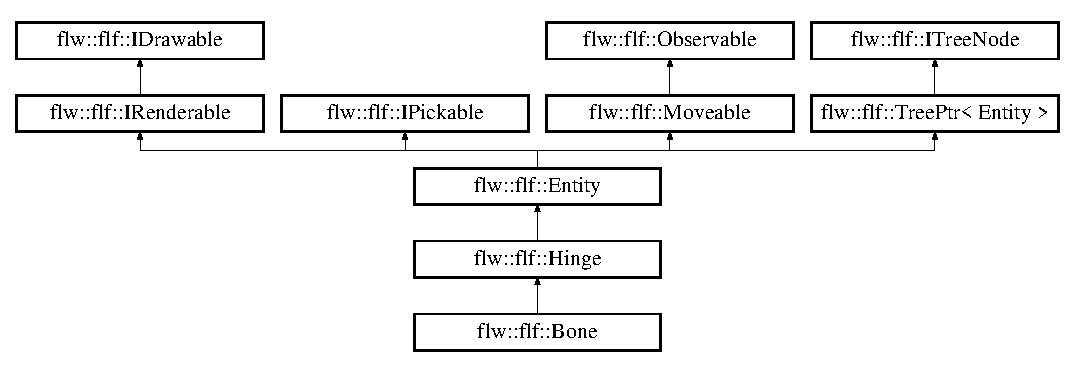
\includegraphics[height=4.487180cm]{classflw_1_1flf_1_1Bone}
\end{center}
\end{figure}
\subsection*{Public Member Functions}
\begin{DoxyCompactItemize}
\item 
{\bfseries Bone} (ai\+Bone $\ast$assimp\+Bone)\hypertarget{classflw_1_1flf_1_1Bone_a392042b750cc4bf561825ee302202fb5}{}\label{classflw_1_1flf_1_1Bone_a392042b750cc4bf561825ee302202fb5}

\item 
std\+::string {\bfseries get\+Name} () const \hypertarget{classflw_1_1flf_1_1Bone_aa3d313fe671f82035501e9d861bfe8e9}{}\label{classflw_1_1flf_1_1Bone_aa3d313fe671f82035501e9d861bfe8e9}

\item 
glm\+::mat4 {\bfseries get\+Offset\+Matrix} () const \hypertarget{classflw_1_1flf_1_1Bone_ab3a2ea61469a5073849c474bea100820}{}\label{classflw_1_1flf_1_1Bone_ab3a2ea61469a5073849c474bea100820}

\item 
glm\+::mat4 {\bfseries get\+Global\+Offset\+Matrix} () const \hypertarget{classflw_1_1flf_1_1Bone_a017830c8a7fafbb3823114b65e9467a1}{}\label{classflw_1_1flf_1_1Bone_a017830c8a7fafbb3823114b65e9467a1}

\item 
void {\bfseries set\+Name} (std\+::string name)\hypertarget{classflw_1_1flf_1_1Bone_a6cf797dea162d2c87716ba961501b3f6}{}\label{classflw_1_1flf_1_1Bone_a6cf797dea162d2c87716ba961501b3f6}

\item 
void {\bfseries set\+Offset\+Matrix} (glm\+::mat4 m)\hypertarget{classflw_1_1flf_1_1Bone_a457c06cf7d1b77cf6a88e95800c13cf0}{}\label{classflw_1_1flf_1_1Bone_a457c06cf7d1b77cf6a88e95800c13cf0}

\item 
void {\bfseries set\+Global\+Offset\+Matrix} (glm\+::mat4 m)\hypertarget{classflw_1_1flf_1_1Bone_a32ce1f1f71f73a92e2916ff83b721e54}{}\label{classflw_1_1flf_1_1Bone_a32ce1f1f71f73a92e2916ff83b721e54}

\item 
void {\bfseries log} () const override\hypertarget{classflw_1_1flf_1_1Bone_ae1a421ceb6ee7d32bb01aa7f388c15a4}{}\label{classflw_1_1flf_1_1Bone_ae1a421ceb6ee7d32bb01aa7f388c15a4}

\end{DoxyCompactItemize}
\subsection*{Additional Inherited Members}


\subsection{Detailed Description}
\hyperlink{classflw_1_1flf_1_1Hinge}{Hinge} used by \hyperlink{classflw_1_1flf_1_1Animator}{Animator} to populate bone transformations. 

The documentation for this class was generated from the following file\+:\begin{DoxyCompactItemize}
\item 
/home/filip/\+Projects/fillwave/inc/fillwave/models/animations/Bone.\+h\end{DoxyCompactItemize}

\hypertarget{classflw_1_1flf_1_1BoostColor}{}\section{flw\+:\+:flf\+:\+:Boost\+Color Class Reference}
\label{classflw_1_1flf_1_1BoostColor}\index{flw\+::flf\+::\+Boost\+Color@{flw\+::flf\+::\+Boost\+Color}}


Effect to boost the models color.  




{\ttfamily \#include $<$Boost\+Color.\+h$>$}

Inheritance diagram for flw\+:\+:flf\+:\+:Boost\+Color\+:\begin{figure}[H]
\begin{center}
\leavevmode
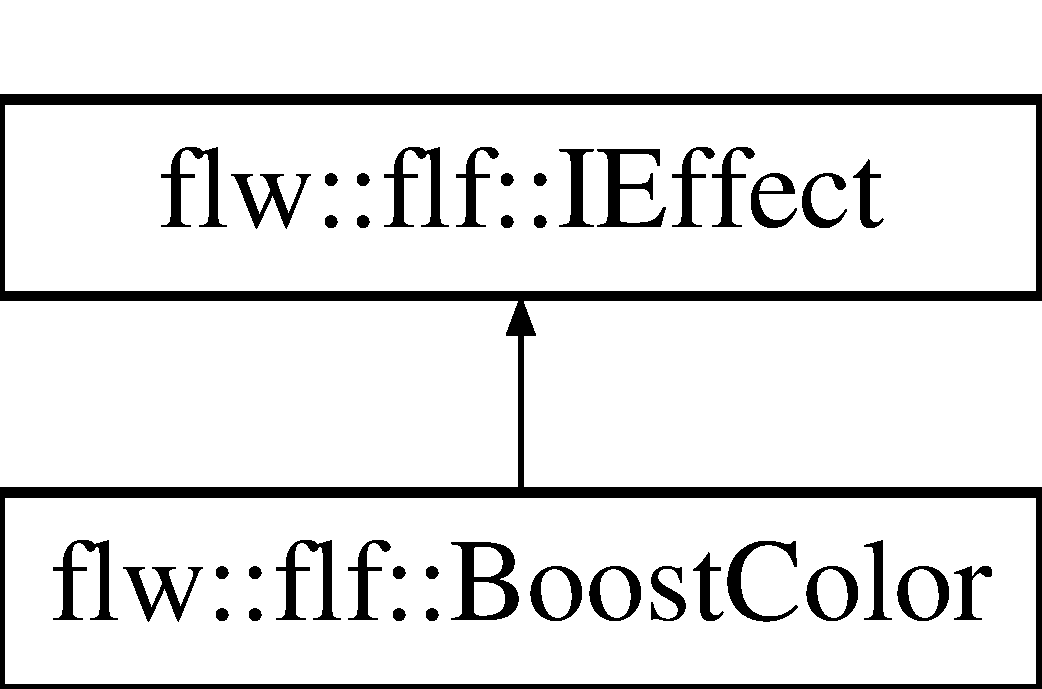
\includegraphics[height=2.000000cm]{classflw_1_1flf_1_1BoostColor}
\end{center}
\end{figure}
\subsection*{Public Member Functions}
\begin{DoxyCompactItemize}
\item 
{\bfseries Boost\+Color} (G\+Lfloat boost=1.\+0f)\hypertarget{classflw_1_1flf_1_1BoostColor_a2440c2e5456e839fa68d5b0b7a777383}{}\label{classflw_1_1flf_1_1BoostColor_a2440c2e5456e839fa68d5b0b7a777383}

\item 
void \hyperlink{classflw_1_1flf_1_1BoostColor_a254c40ad807688df7bc7c8a2b8735338}{pre\+Draw\+Action} (\hyperlink{classflw_1_1flc_1_1Program}{flc\+::\+Program} $\ast$program) override
\begin{DoxyCompactList}\small\item\em virtual\+: defines action to be done just before the draw. \end{DoxyCompactList}\item 
void \hyperlink{classflw_1_1flf_1_1BoostColor_a8ef5c9e32f4b210a4240d454021e4408}{post\+Draw\+Action} (\hyperlink{classflw_1_1flc_1_1Program}{flc\+::\+Program} $\ast$program) override
\begin{DoxyCompactList}\small\item\em virtual\+: defines action to be done just after the draw. \end{DoxyCompactList}\item 
void \hyperlink{classflw_1_1flf_1_1BoostColor_a80c34ed26ed847e39fc036baad24e1d5}{stop\+Action} (\hyperlink{classflw_1_1flc_1_1Program}{flc\+::\+Program} $\ast$program) override
\begin{DoxyCompactList}\small\item\em virtual\+: defines action to be done when the effect is stopped. \end{DoxyCompactList}\item 
void \hyperlink{classflw_1_1flf_1_1BoostColor_a4bd0b925fea15ce7fc00296e3d2672e6}{start\+Action} (\hyperlink{classflw_1_1flc_1_1Program}{flc\+::\+Program} $\ast$program) override
\begin{DoxyCompactList}\small\item\em virtual\+: defines action to be done when the effect is started. \end{DoxyCompactList}\end{DoxyCompactItemize}


\subsection{Detailed Description}
Effect to boost the models color. 

\subsection{Member Function Documentation}
\index{flw\+::flf\+::\+Boost\+Color@{flw\+::flf\+::\+Boost\+Color}!post\+Draw\+Action@{post\+Draw\+Action}}
\index{post\+Draw\+Action@{post\+Draw\+Action}!flw\+::flf\+::\+Boost\+Color@{flw\+::flf\+::\+Boost\+Color}}
\subsubsection[{\texorpdfstring{post\+Draw\+Action(flc\+::\+Program $\ast$program) override}{postDrawAction(flc::Program *program) override}}]{\setlength{\rightskip}{0pt plus 5cm}void flw\+::flf\+::\+Boost\+Color\+::post\+Draw\+Action (
\begin{DoxyParamCaption}
\item[{{\bf flc\+::\+Program} $\ast$}]{program}
\end{DoxyParamCaption}
)\hspace{0.3cm}{\ttfamily [override]}, {\ttfamily [virtual]}}\hypertarget{classflw_1_1flf_1_1BoostColor_a8ef5c9e32f4b210a4240d454021e4408}{}\label{classflw_1_1flf_1_1BoostColor_a8ef5c9e32f4b210a4240d454021e4408}


virtual\+: defines action to be done just after the draw. 

post\+Draw\+Action 

Implements \hyperlink{classflw_1_1flf_1_1IEffect_a6bb11d90e7e4da057ca398bd8c61208a}{flw\+::flf\+::\+I\+Effect}.

\index{flw\+::flf\+::\+Boost\+Color@{flw\+::flf\+::\+Boost\+Color}!pre\+Draw\+Action@{pre\+Draw\+Action}}
\index{pre\+Draw\+Action@{pre\+Draw\+Action}!flw\+::flf\+::\+Boost\+Color@{flw\+::flf\+::\+Boost\+Color}}
\subsubsection[{\texorpdfstring{pre\+Draw\+Action(flc\+::\+Program $\ast$program) override}{preDrawAction(flc::Program *program) override}}]{\setlength{\rightskip}{0pt plus 5cm}void flw\+::flf\+::\+Boost\+Color\+::pre\+Draw\+Action (
\begin{DoxyParamCaption}
\item[{{\bf flc\+::\+Program} $\ast$}]{program}
\end{DoxyParamCaption}
)\hspace{0.3cm}{\ttfamily [override]}, {\ttfamily [virtual]}}\hypertarget{classflw_1_1flf_1_1BoostColor_a254c40ad807688df7bc7c8a2b8735338}{}\label{classflw_1_1flf_1_1BoostColor_a254c40ad807688df7bc7c8a2b8735338}


virtual\+: defines action to be done just before the draw. 

pre\+Draw\+Action 

Implements \hyperlink{classflw_1_1flf_1_1IEffect_ae65eed21e40a226c7739d3c5dedd9e50}{flw\+::flf\+::\+I\+Effect}.

\index{flw\+::flf\+::\+Boost\+Color@{flw\+::flf\+::\+Boost\+Color}!start\+Action@{start\+Action}}
\index{start\+Action@{start\+Action}!flw\+::flf\+::\+Boost\+Color@{flw\+::flf\+::\+Boost\+Color}}
\subsubsection[{\texorpdfstring{start\+Action(flc\+::\+Program $\ast$program) override}{startAction(flc::Program *program) override}}]{\setlength{\rightskip}{0pt plus 5cm}void flw\+::flf\+::\+Boost\+Color\+::start\+Action (
\begin{DoxyParamCaption}
\item[{{\bf flc\+::\+Program} $\ast$}]{program}
\end{DoxyParamCaption}
)\hspace{0.3cm}{\ttfamily [override]}, {\ttfamily [virtual]}}\hypertarget{classflw_1_1flf_1_1BoostColor_a4bd0b925fea15ce7fc00296e3d2672e6}{}\label{classflw_1_1flf_1_1BoostColor_a4bd0b925fea15ce7fc00296e3d2672e6}


virtual\+: defines action to be done when the effect is started. 

start\+Action 

Implements \hyperlink{classflw_1_1flf_1_1IEffect_afc7cec9080d135ed264b08a90c7b94e9}{flw\+::flf\+::\+I\+Effect}.

\index{flw\+::flf\+::\+Boost\+Color@{flw\+::flf\+::\+Boost\+Color}!stop\+Action@{stop\+Action}}
\index{stop\+Action@{stop\+Action}!flw\+::flf\+::\+Boost\+Color@{flw\+::flf\+::\+Boost\+Color}}
\subsubsection[{\texorpdfstring{stop\+Action(flc\+::\+Program $\ast$program) override}{stopAction(flc::Program *program) override}}]{\setlength{\rightskip}{0pt plus 5cm}void flw\+::flf\+::\+Boost\+Color\+::stop\+Action (
\begin{DoxyParamCaption}
\item[{{\bf flc\+::\+Program} $\ast$}]{program}
\end{DoxyParamCaption}
)\hspace{0.3cm}{\ttfamily [override]}, {\ttfamily [virtual]}}\hypertarget{classflw_1_1flf_1_1BoostColor_a80c34ed26ed847e39fc036baad24e1d5}{}\label{classflw_1_1flf_1_1BoostColor_a80c34ed26ed847e39fc036baad24e1d5}


virtual\+: defines action to be done when the effect is stopped. 

stop\+Action 

Implements \hyperlink{classflw_1_1flf_1_1IEffect_a1a03eaf63a9d4edbd8764540d2d4133c}{flw\+::flf\+::\+I\+Effect}.



The documentation for this class was generated from the following file\+:\begin{DoxyCompactItemize}
\item 
/home/filip/\+Projects/fillwave/inc/fillwave/models/effects/Boost\+Color.\+h\end{DoxyCompactItemize}

\hypertarget{classflw_1_1flf_1_1Box}{}\section{flw\+:\+:flf\+:\+:Box Class Reference}
\label{classflw_1_1flf_1_1Box}\index{flw\+::flf\+::\+Box@{flw\+::flf\+::\+Box}}


Basic \hyperlink{classflw_1_1flf_1_1Shape}{Shape} for general usage. Indices and vertices provided.  




{\ttfamily \#include $<$Box.\+h$>$}

Inheritance diagram for flw\+:\+:flf\+:\+:Box\+:\begin{figure}[H]
\begin{center}
\leavevmode
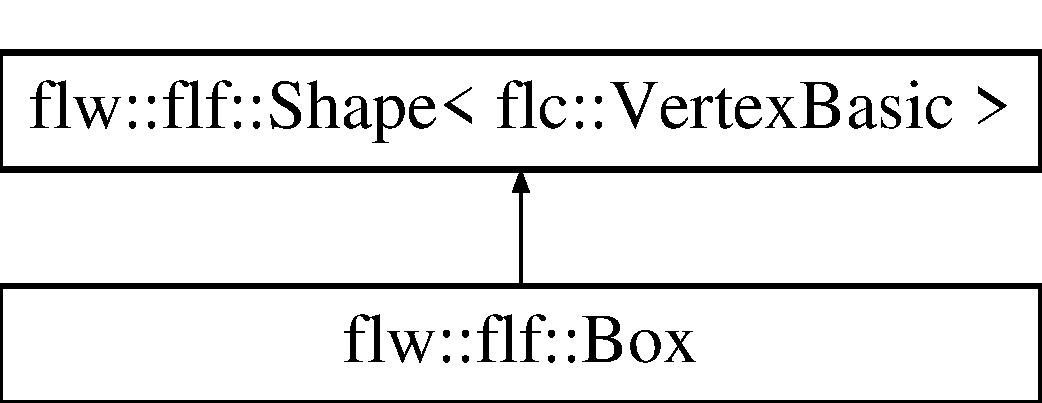
\includegraphics[height=2.000000cm]{classflw_1_1flf_1_1Box}
\end{center}
\end{figure}
\subsection*{Public Member Functions}
\begin{DoxyCompactItemize}
\item 
{\bfseries Box} (G\+Lfloat quad\+Size=1.\+0f)\hypertarget{classflw_1_1flf_1_1Box_a1810262c6b67eb89f6780b6c1513fd13}{}\label{classflw_1_1flf_1_1Box_a1810262c6b67eb89f6780b6c1513fd13}

\item 
void {\bfseries generate\+Vertices} ()\hypertarget{classflw_1_1flf_1_1Box_a3c136b1b3d75e5a79c86136074c93cf7}{}\label{classflw_1_1flf_1_1Box_a3c136b1b3d75e5a79c86136074c93cf7}

\item 
void {\bfseries generate\+Side} ()\hypertarget{classflw_1_1flf_1_1Box_a3c137640c604691d4398293e0a8b7382}{}\label{classflw_1_1flf_1_1Box_a3c137640c604691d4398293e0a8b7382}

\item 
void {\bfseries generate\+Indices} ()\hypertarget{classflw_1_1flf_1_1Box_a0b8cc4c091b5e086cb510a25bd462a62}{}\label{classflw_1_1flf_1_1Box_a0b8cc4c091b5e086cb510a25bd462a62}

\end{DoxyCompactItemize}
\subsection*{Additional Inherited Members}


\subsection{Detailed Description}
Basic \hyperlink{classflw_1_1flf_1_1Shape}{Shape} for general usage. Indices and vertices provided. 

The documentation for this class was generated from the following file\+:\begin{DoxyCompactItemize}
\item 
/home/filip/\+Projects/fillwave/inc/fillwave/models/shapes/Box.\+h\end{DoxyCompactItemize}

\hypertarget{classflw_1_1flf_1_1BoxOcclusion}{}\section{flw\+:\+:flf\+:\+:Box\+Occlusion Class Reference}
\label{classflw_1_1flf_1_1BoxOcclusion}\index{flw\+::flf\+::\+Box\+Occlusion@{flw\+::flf\+::\+Box\+Occlusion}}


Basic \hyperlink{classflw_1_1flf_1_1Shape}{Shape} for specific usage, providing each model to participate in OQ algorithm.  




{\ttfamily \#include $<$Box\+Occlusion.\+h$>$}

Inheritance diagram for flw\+:\+:flf\+:\+:Box\+Occlusion\+:\begin{figure}[H]
\begin{center}
\leavevmode
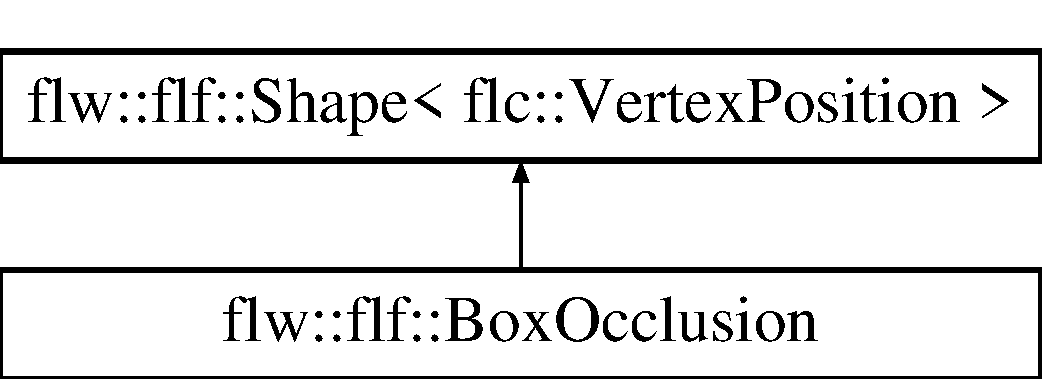
\includegraphics[height=2.000000cm]{classflw_1_1flf_1_1BoxOcclusion}
\end{center}
\end{figure}
\subsection*{Public Member Functions}
\begin{DoxyCompactItemize}
\item 
\mbox{\Hypertarget{classflw_1_1flf_1_1BoxOcclusion_a8c6897ee2fc8384490f2a78714004ff9}\label{classflw_1_1flf_1_1BoxOcclusion_a8c6897ee2fc8384490f2a78714004ff9}} 
{\bfseries Box\+Occlusion} (G\+Lfloat quad\+Size=1.\+0f)
\end{DoxyCompactItemize}
\subsection*{Additional Inherited Members}


\subsection{Detailed Description}
Basic \hyperlink{classflw_1_1flf_1_1Shape}{Shape} for specific usage, providing each model to participate in OQ algorithm. 

The documentation for this class was generated from the following file\+:\begin{DoxyCompactItemize}
\item 
/home/filip/projects/fillwave/inc/fillwave/models/shapes/Box\+Occlusion.\+h\end{DoxyCompactItemize}

\hypertarget{structflw_1_1flf_1_1BufferSystem}{}\section{flw\+:\+:flf\+:\+:Buffer\+System Class Reference}
\label{structflw_1_1flf_1_1BufferSystem}\index{flw\+::flf\+::\+Buffer\+System@{flw\+::flf\+::\+Buffer\+System}}


Connects V\+AO pointer and V\+AO\textquotesingle{}s user pointer in single class.  




{\ttfamily \#include $<$Buffer\+System.\+h$>$}

\subsection*{Public Attributes}
\begin{DoxyCompactItemize}
\item 
\hyperlink{classflw_1_1flf_1_1TCache}{T\+Cache}$<$ M\+A\+X\+\_\+\+C\+A\+C\+H\+E\+\_\+\+S\+I\+ZE, \hyperlink{classflw_1_1flc_1_1VertexArray}{flc\+::\+Vertex\+Array}, \hyperlink{classflw_1_1flf_1_1IReloadable}{I\+Reloadable} $\ast$ $>$ {\bfseries m\+Vertex\+Arrays}\hypertarget{structflw_1_1flf_1_1BufferSystem_a7974ca27bdeeb1606fb34d54a9f828fa}{}\label{structflw_1_1flf_1_1BufferSystem_a7974ca27bdeeb1606fb34d54a9f828fa}

\item 
\hyperlink{classflw_1_1flf_1_1TCache}{T\+Cache}$<$ M\+A\+X\+\_\+\+C\+A\+C\+H\+E\+\_\+\+S\+I\+ZE, \hyperlink{classflw_1_1flc_1_1VertexBufferBasic}{flc\+::\+Vertex\+Buffer\+Basic}, \hyperlink{classflw_1_1flc_1_1VertexArray}{flc\+::\+Vertex\+Array} $\ast$, \hyperlink{classflw_1_1flf_1_1TerrainConstructor}{flf\+::\+Terrain\+Constructor} $\ast$, G\+Lint, G\+Lfloat, std\+::vector$<$ G\+Luint $>$ \& $>$ {\bfseries m\+Vertices}\hypertarget{structflw_1_1flf_1_1BufferSystem_ada93731ae4c7155525f3d4961e329a54}{}\label{structflw_1_1flf_1_1BufferSystem_ada93731ae4c7155525f3d4961e329a54}

\item 
\hyperlink{classflw_1_1flf_1_1TCache}{T\+Cache}$<$ M\+A\+X\+\_\+\+C\+A\+C\+H\+E\+\_\+\+S\+I\+ZE, \hyperlink{classflw_1_1flc_1_1IndexBuffer}{flc\+::\+Index\+Buffer}, \hyperlink{classflw_1_1flc_1_1VertexArray}{flc\+::\+Vertex\+Array} $\ast$, std\+::vector$<$ G\+Luint $>$ \& $>$ {\bfseries m\+Indices}\hypertarget{structflw_1_1flf_1_1BufferSystem_a0e8fe9e2c159bedf179376db8406a12d}{}\label{structflw_1_1flf_1_1BufferSystem_a0e8fe9e2c159bedf179376db8406a12d}

\item 
\hyperlink{classflw_1_1flf_1_1TCache}{T\+Cache}$<$ M\+A\+X\+\_\+\+C\+A\+C\+H\+E\+\_\+\+S\+I\+ZE, \hyperlink{classflw_1_1flc_1_1VertexBufferText}{flc\+::\+Vertex\+Buffer\+Text}, \hyperlink{classflw_1_1flc_1_1VertexArray}{flc\+::\+Vertex\+Array} $\ast$, const std\+::vector$<$ G\+Lfloat $>$ \&, const std\+::vector$<$ G\+Lfloat $>$ \& $>$ {\bfseries m\+Vertices\+Text}\hypertarget{structflw_1_1flf_1_1BufferSystem_a9f8c063d64ae750b96f9fb2f64fed774}{}\label{structflw_1_1flf_1_1BufferSystem_a9f8c063d64ae750b96f9fb2f64fed774}

\item 
\hyperlink{classflw_1_1flf_1_1TCache}{T\+Cache}$<$ M\+A\+X\+\_\+\+C\+A\+C\+H\+E\+\_\+\+S\+I\+ZE, std\+::vector$<$ \hyperlink{classflw_1_1flc_1_1VertexBufferParticlesGPU}{flc\+::\+Vertex\+Buffer\+Particles\+G\+PU} $\ast$ $>$, \hyperlink{classflw_1_1flc_1_1VertexArray}{flc\+::\+Vertex\+Array} $\ast$, std\+::vector$<$ \hyperlink{structflw_1_1flc_1_1VertexParticleGPU}{flc\+::\+Vertex\+Particle\+G\+PU} $>$ \& $>$ {\bfseries m\+Vertices\+Particles\+G\+PU}\hypertarget{structflw_1_1flf_1_1BufferSystem_afd8dce391dc910999a16c4fdd53a79e3}{}\label{structflw_1_1flf_1_1BufferSystem_afd8dce391dc910999a16c4fdd53a79e3}

\item 
\hyperlink{classflw_1_1flf_1_1TCache}{T\+Cache}$<$ M\+A\+X\+\_\+\+C\+A\+C\+H\+E\+\_\+\+S\+I\+ZE, \hyperlink{classflw_1_1flc_1_1VertexBufferParticles}{flc\+::\+Vertex\+Buffer\+Particles}, \hyperlink{classflw_1_1flc_1_1VertexArray}{flc\+::\+Vertex\+Array} $\ast$, std\+::vector$<$ G\+Lfloat $>$ \&, std\+::vector$<$ G\+Lfloat $>$ \&, std\+::vector$<$ G\+Lfloat $>$ \& $>$ {\bfseries m\+Vertices\+Particles}\hypertarget{structflw_1_1flf_1_1BufferSystem_a75dd883faa9d491424ab2a8dcb75abee}{}\label{structflw_1_1flf_1_1BufferSystem_a75dd883faa9d491424ab2a8dcb75abee}

\item 
\hyperlink{classflw_1_1flf_1_1TCache}{T\+Cache}$<$ M\+A\+X\+\_\+\+C\+A\+C\+H\+E\+\_\+\+S\+I\+ZE, \hyperlink{classflw_1_1flc_1_1VertexBufferDebug}{flc\+::\+Vertex\+Buffer\+Debug}, \hyperlink{classflw_1_1flc_1_1VertexArray}{flc\+::\+Vertex\+Array} $\ast$, G\+Lfloat $>$ {\bfseries m\+Vertices\+Debugger}\hypertarget{structflw_1_1flf_1_1BufferSystem_a36720b705108842100c58f19793c3878}{}\label{structflw_1_1flf_1_1BufferSystem_a36720b705108842100c58f19793c3878}

\item 
\hyperlink{classflw_1_1flf_1_1TCache}{T\+Cache}$<$ M\+A\+X\+\_\+\+C\+A\+C\+H\+E\+\_\+\+S\+I\+ZE, \hyperlink{classflw_1_1flc_1_1VertexBufferFloat}{flc\+::\+Vertex\+Buffer\+Float}, \hyperlink{classflw_1_1flc_1_1VertexArray}{flc\+::\+Vertex\+Array} $\ast$, std\+::vector$<$ \hyperlink{structflw_1_1flc_1_1VertexFloat}{flc\+::\+Vertex\+Float} $>$ \& $>$ {\bfseries m\+Vertices\+Float}\hypertarget{structflw_1_1flf_1_1BufferSystem_a315fe65dc1c97c15215d09627a4d3463}{}\label{structflw_1_1flf_1_1BufferSystem_a315fe65dc1c97c15215d09627a4d3463}

\item 
\hyperlink{classflw_1_1flf_1_1TCache}{T\+Cache}$<$ M\+A\+X\+\_\+\+C\+A\+C\+H\+E\+\_\+\+S\+I\+ZE, \hyperlink{classflw_1_1flc_1_1VertexBufferPosition}{flc\+::\+Vertex\+Buffer\+Position}, \hyperlink{classflw_1_1flc_1_1VertexArray}{flc\+::\+Vertex\+Array} $\ast$, std\+::vector$<$ \hyperlink{structflw_1_1flc_1_1VertexPosition}{flc\+::\+Vertex\+Position} $>$ \& $>$ {\bfseries m\+Vertices\+Position}\hypertarget{structflw_1_1flf_1_1BufferSystem_aa90f229de2f3f3237ae6328d170b9dd0}{}\label{structflw_1_1flf_1_1BufferSystem_aa90f229de2f3f3237ae6328d170b9dd0}

\end{DoxyCompactItemize}


\subsection{Detailed Description}
Connects V\+AO pointer and V\+AO\textquotesingle{}s user pointer in single class. 

The documentation for this class was generated from the following file\+:\begin{DoxyCompactItemize}
\item 
/home/filip/\+Projects/fillwave/inc/fillwave/management/Buffer\+System.\+h\end{DoxyCompactItemize}

\hypertarget{classflw_1_1flf_1_1BuilderEmiter}{}\section{flw\+:\+:flf\+:\+:Builder\+Emiter Class Reference}
\label{classflw_1_1flf_1_1BuilderEmiter}\index{flw\+::flf\+::\+Builder\+Emiter@{flw\+::flf\+::\+Builder\+Emiter}}


\hyperlink{classflw_1_1flf_1_1BuilderModel}{Builder\+Model} which builds the particles emiter.  




{\ttfamily \#include $<$Builder\+Emiter.\+h$>$}

\subsection*{Public Member Functions}
\begin{DoxyCompactItemize}
\item 
{\bfseries Builder\+Emiter} (\hyperlink{classflw_1_1Engine}{Engine} $\ast$engine)\hypertarget{classflw_1_1flf_1_1BuilderEmiter_ae0eee2b4840fa09408e0e7eead1dc694}{}\label{classflw_1_1flf_1_1BuilderEmiter_ae0eee2b4840fa09408e0e7eead1dc694}

\item 
\hyperlink{classflw_1_1flf_1_1BuilderEmiter}{Builder\+Emiter} \& {\bfseries set\+Emiting\+Source\+Rate} (G\+Lfloat emiting\+Source\+Rate)\hypertarget{classflw_1_1flf_1_1BuilderEmiter_a554c839b5c60595e4b1d04d9d1b9095b}{}\label{classflw_1_1flf_1_1BuilderEmiter_a554c839b5c60595e4b1d04d9d1b9095b}

\item 
\hyperlink{classflw_1_1flf_1_1BuilderEmiter}{Builder\+Emiter} \& {\bfseries set\+How\+Many} (G\+Luint howmany)\hypertarget{classflw_1_1flf_1_1BuilderEmiter_af64e3d7700f5e12fc976ea90aa518071}{}\label{classflw_1_1flf_1_1BuilderEmiter_af64e3d7700f5e12fc976ea90aa518071}

\item 
\hyperlink{classflw_1_1flf_1_1BuilderEmiter}{Builder\+Emiter} \& {\bfseries set\+Color} (glm\+::vec4 color)\hypertarget{classflw_1_1flf_1_1BuilderEmiter_a3ffc7c438025abc17b1e1d9bee723d60}{}\label{classflw_1_1flf_1_1BuilderEmiter_a3ffc7c438025abc17b1e1d9bee723d60}

\item 
\hyperlink{classflw_1_1flf_1_1BuilderEmiter}{Builder\+Emiter} \& {\bfseries set\+Acceleration} (glm\+::vec3 acceleration)\hypertarget{classflw_1_1flf_1_1BuilderEmiter_a6ca384523af8e0acdcf4bc92c19d3421}{}\label{classflw_1_1flf_1_1BuilderEmiter_a6ca384523af8e0acdcf4bc92c19d3421}

\item 
\hyperlink{classflw_1_1flf_1_1BuilderEmiter}{Builder\+Emiter} \& {\bfseries set\+Start\+Velocity} (glm\+::vec3 start\+Velocity)\hypertarget{classflw_1_1flf_1_1BuilderEmiter_a157e33bb34dd0d524c701be21342f5a9}{}\label{classflw_1_1flf_1_1BuilderEmiter_a157e33bb34dd0d524c701be21342f5a9}

\item 
\hyperlink{classflw_1_1flf_1_1BuilderEmiter}{Builder\+Emiter} \& {\bfseries set\+Robustness\+Velocity} (glm\+::vec3 robustness\+Velocity)\hypertarget{classflw_1_1flf_1_1BuilderEmiter_ab5fa5784fa08efb3b496efb4edbd44ca}{}\label{classflw_1_1flf_1_1BuilderEmiter_ab5fa5784fa08efb3b496efb4edbd44ca}

\item 
\hyperlink{classflw_1_1flf_1_1BuilderEmiter}{Builder\+Emiter} \& {\bfseries set\+Start\+Position} (glm\+::vec3 start\+Position)\hypertarget{classflw_1_1flf_1_1BuilderEmiter_a67415b33f24dd3546738decdf397a156}{}\label{classflw_1_1flf_1_1BuilderEmiter_a67415b33f24dd3546738decdf397a156}

\item 
\hyperlink{classflw_1_1flf_1_1BuilderEmiter}{Builder\+Emiter} \& {\bfseries set\+Robustness\+Position} (glm\+::vec3 robustness\+Position)\hypertarget{classflw_1_1flf_1_1BuilderEmiter_a175528b261603f4c068742a466c683d6}{}\label{classflw_1_1flf_1_1BuilderEmiter_a175528b261603f4c068742a466c683d6}

\item 
\hyperlink{classflw_1_1flf_1_1BuilderEmiter}{Builder\+Emiter} \& {\bfseries set\+Start\+Size} (G\+Lfloat size)\hypertarget{classflw_1_1flf_1_1BuilderEmiter_aa15293c9c54677d2d8681b0554054c5f}{}\label{classflw_1_1flf_1_1BuilderEmiter_aa15293c9c54677d2d8681b0554054c5f}

\item 
\hyperlink{classflw_1_1flf_1_1BuilderEmiter}{Builder\+Emiter} \& {\bfseries set\+Lifetime} (G\+Lfloat lifetime)\hypertarget{classflw_1_1flf_1_1BuilderEmiter_ab6a83e1908dff2d44383a623150e05fd}{}\label{classflw_1_1flf_1_1BuilderEmiter_ab6a83e1908dff2d44383a623150e05fd}

\item 
\hyperlink{classflw_1_1flf_1_1BuilderEmiter}{Builder\+Emiter} \& {\bfseries set\+Texture} (\hyperlink{classflw_1_1flc_1_1Texture}{flc\+::\+Texture} $\ast$texture)\hypertarget{classflw_1_1flf_1_1BuilderEmiter_a475b844ff412679844ad119fa2089fbf}{}\label{classflw_1_1flf_1_1BuilderEmiter_a475b844ff412679844ad119fa2089fbf}

\item 
\hyperlink{classflw_1_1flf_1_1BuilderEmiter}{Builder\+Emiter} \& {\bfseries set\+Blending\+Source} (G\+Lenum source\+Color)\hypertarget{classflw_1_1flf_1_1BuilderEmiter_a27f8b3e2804ff47162fe2731cc167bf0}{}\label{classflw_1_1flf_1_1BuilderEmiter_a27f8b3e2804ff47162fe2731cc167bf0}

\item 
\hyperlink{classflw_1_1flf_1_1BuilderEmiter}{Builder\+Emiter} \& {\bfseries set\+Blending\+Destination} (G\+Lenum destination\+Color)\hypertarget{classflw_1_1flf_1_1BuilderEmiter_a14e4f56ea5d30c1495bf0affa80ed4d6}{}\label{classflw_1_1flf_1_1BuilderEmiter_a14e4f56ea5d30c1495bf0affa80ed4d6}

\item 
\hyperlink{classflw_1_1flf_1_1BuilderEmiter}{Builder\+Emiter} \& {\bfseries set\+Depth\+Testing} (G\+Lboolean depth\+Testing)\hypertarget{classflw_1_1flf_1_1BuilderEmiter_a03b51afcbae7f0a4506273d3e02d8dfd}{}\label{classflw_1_1flf_1_1BuilderEmiter_a03b51afcbae7f0a4506273d3e02d8dfd}

\item 
\hyperlink{classflw_1_1flf_1_1BuilderEmiter}{Builder\+Emiter} \& {\bfseries set\+Alpha\+Cut\+Off} (G\+Lfloat cut\+Off\+Level)\hypertarget{classflw_1_1flf_1_1BuilderEmiter_ae5272c6a780830b691fda1a58e387ee1}{}\label{classflw_1_1flf_1_1BuilderEmiter_ae5272c6a780830b691fda1a58e387ee1}

\item 
pu\+I\+Emiter\+Point {\bfseries build\+Emiter\+G\+PU} ()\hypertarget{classflw_1_1flf_1_1BuilderEmiter_aadeaaee36e99644da1df706fee362219}{}\label{classflw_1_1flf_1_1BuilderEmiter_aadeaaee36e99644da1df706fee362219}

\item 
pu\+I\+Emiter\+Point {\bfseries build\+Emiter\+C\+PU} ()\hypertarget{classflw_1_1flf_1_1BuilderEmiter_ab42b38f7eb290dac2b6282b191dec767}{}\label{classflw_1_1flf_1_1BuilderEmiter_ab42b38f7eb290dac2b6282b191dec767}

\end{DoxyCompactItemize}


\subsection{Detailed Description}
\hyperlink{classflw_1_1flf_1_1BuilderModel}{Builder\+Model} which builds the particles emiter. 

The documentation for this class was generated from the following file\+:\begin{DoxyCompactItemize}
\item 
/home/filip/\+Projects/fillwave/inc/fillwave/models/builders/Builder\+Emiter.\+h\end{DoxyCompactItemize}

\hypertarget{classflw_1_1flf_1_1BuilderModel}{}\section{flw\+:\+:flf\+:\+:Builder\+Model Class Reference}
\label{classflw_1_1flf_1_1BuilderModel}\index{flw\+::flf\+::\+Builder\+Model@{flw\+::flf\+::\+Builder\+Model}}


Builder which builds the model from the asset file.  




{\ttfamily \#include $<$Builder\+Model.\+h$>$}

Inheritance diagram for flw\+:\+:flf\+:\+:Builder\+Model\+:\begin{figure}[H]
\begin{center}
\leavevmode
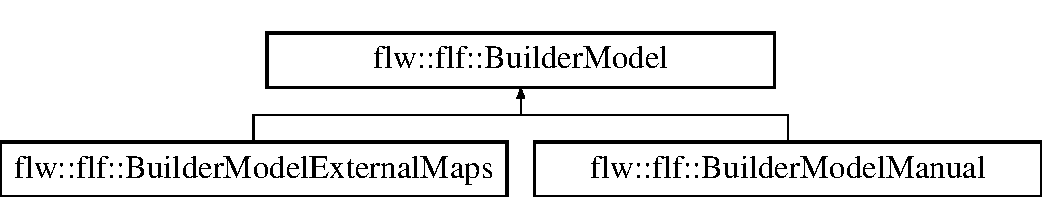
\includegraphics[height=2.000000cm]{classflw_1_1flf_1_1BuilderModel}
\end{center}
\end{figure}
\subsection*{Public Member Functions}
\begin{DoxyCompactItemize}
\item 
{\bfseries Builder\+Model} (\hyperlink{classflw_1_1Engine}{Engine} $\ast$engine, std\+::string model\+Path, \hyperlink{classflw_1_1flc_1_1Program}{flc\+::\+Program} $\ast$program)\hypertarget{classflw_1_1flf_1_1BuilderModel_a2bdb7cf2baa8140b6a7fe9de8f178ccf}{}\label{classflw_1_1flf_1_1BuilderModel_a2bdb7cf2baa8140b6a7fe9de8f178ccf}

\item 
virtual pu\+Model {\bfseries build} ()\hypertarget{classflw_1_1flf_1_1BuilderModel_ab5ec429a3559b7b4f0aff98980106805}{}\label{classflw_1_1flf_1_1BuilderModel_ab5ec429a3559b7b4f0aff98980106805}

\item 
\hyperlink{classflw_1_1flf_1_1BuilderModel}{Builder\+Model} \& {\bfseries set\+Model\+Path} (std\+::string \&path)\hypertarget{classflw_1_1flf_1_1BuilderModel_a049974f188c679dbf4ef514ccad13f68}{}\label{classflw_1_1flf_1_1BuilderModel_a049974f188c679dbf4ef514ccad13f68}

\item 
\hyperlink{classflw_1_1flf_1_1BuilderModel}{Builder\+Model} \& {\bfseries set\+Program} (\hyperlink{classflw_1_1flc_1_1Program}{flc\+::\+Program} $\ast$program)\hypertarget{classflw_1_1flf_1_1BuilderModel_a274c0199bf3197984efe7847a4d2052c}{}\label{classflw_1_1flf_1_1BuilderModel_a274c0199bf3197984efe7847a4d2052c}

\end{DoxyCompactItemize}
\subsection*{Protected Attributes}
\begin{DoxyCompactItemize}
\item 
\hyperlink{classflw_1_1Engine}{Engine} $\ast$ {\bfseries m\+Engine}\hypertarget{classflw_1_1flf_1_1BuilderModel_a625e6c302b14ff9775e9ffe3a72b36cb}{}\label{classflw_1_1flf_1_1BuilderModel_a625e6c302b14ff9775e9ffe3a72b36cb}

\item 
\hyperlink{classflw_1_1flc_1_1Program}{flc\+::\+Program} $\ast$ {\bfseries m\+Program}\hypertarget{classflw_1_1flf_1_1BuilderModel_a1ff36d61e2f4ae3e8778293285516a57}{}\label{classflw_1_1flf_1_1BuilderModel_a1ff36d61e2f4ae3e8778293285516a57}

\item 
std\+::string {\bfseries m\+Shape\+Path}\hypertarget{classflw_1_1flf_1_1BuilderModel_ae4afbfefc5abc67be6d88a85dc285df7}{}\label{classflw_1_1flf_1_1BuilderModel_ae4afbfefc5abc67be6d88a85dc285df7}

\end{DoxyCompactItemize}


\subsection{Detailed Description}
Builder which builds the model from the asset file. 

The documentation for this class was generated from the following file\+:\begin{DoxyCompactItemize}
\item 
/home/filip/\+Projects/fillwave/inc/fillwave/models/builders/Builder\+Model.\+h\end{DoxyCompactItemize}

\hypertarget{classflw_1_1flf_1_1BuilderModelExternalMaps}{}\section{flw\+:\+:flf\+:\+:Builder\+Model\+External\+Maps Class Reference}
\label{classflw_1_1flf_1_1BuilderModelExternalMaps}\index{flw\+::flf\+::\+Builder\+Model\+External\+Maps@{flw\+::flf\+::\+Builder\+Model\+External\+Maps}}


\hyperlink{classflw_1_1flf_1_1BuilderModel}{Builder\+Model} which builds the model from the asset file but uses external texture maps.  




{\ttfamily \#include $<$Builder\+Model\+External\+Maps.\+h$>$}

Inheritance diagram for flw\+:\+:flf\+:\+:Builder\+Model\+External\+Maps\+:\begin{figure}[H]
\begin{center}
\leavevmode
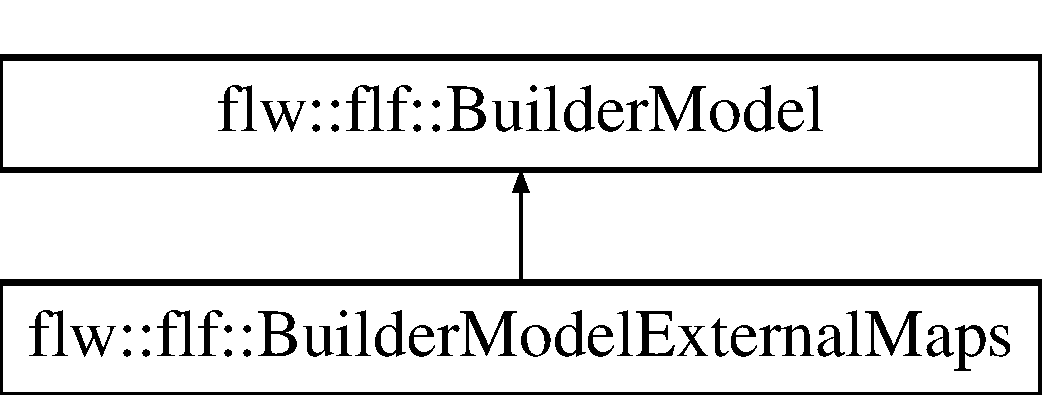
\includegraphics[height=2.000000cm]{classflw_1_1flf_1_1BuilderModelExternalMaps}
\end{center}
\end{figure}
\subsection*{Public Member Functions}
\begin{DoxyCompactItemize}
\item 
\mbox{\Hypertarget{classflw_1_1flf_1_1BuilderModelExternalMaps_ac6426366eb916d358c29949fc50bdc87}\label{classflw_1_1flf_1_1BuilderModelExternalMaps_ac6426366eb916d358c29949fc50bdc87}} 
{\bfseries Builder\+Model\+External\+Maps} (\hyperlink{classflw_1_1Engine}{Engine} $\ast$engine, std\+::string model\+Path=\char`\"{}\char`\"{}, \hyperlink{classflw_1_1flc_1_1Program}{flc\+::\+Program} $\ast$program=nullptr, const std\+::string \&diffuse\+Path=\char`\"{}\char`\"{}, const std\+::string \&normal\+Path=\char`\"{}\char`\"{}, const std\+::string \&specular\+Path=\char`\"{}\char`\"{})
\item 
\mbox{\Hypertarget{classflw_1_1flf_1_1BuilderModelExternalMaps_aca37eea934334c1148447fc6b90cc059}\label{classflw_1_1flf_1_1BuilderModelExternalMaps_aca37eea934334c1148447fc6b90cc059}} 
\hyperlink{classflw_1_1flf_1_1BuilderModel}{Builder\+Model} \& {\bfseries setdiffuse\+Path} (std\+::string \&path)
\item 
\mbox{\Hypertarget{classflw_1_1flf_1_1BuilderModelExternalMaps_a7f2aaf60ece974f81a3457779c9285c9}\label{classflw_1_1flf_1_1BuilderModelExternalMaps_a7f2aaf60ece974f81a3457779c9285c9}} 
\hyperlink{classflw_1_1flf_1_1BuilderModel}{Builder\+Model} \& {\bfseries set\+Normal\+Map\+Path} (std\+::string \&path)
\item 
\mbox{\Hypertarget{classflw_1_1flf_1_1BuilderModelExternalMaps_ae55c925549e30f8161c4e4dfea45a1c2}\label{classflw_1_1flf_1_1BuilderModelExternalMaps_ae55c925549e30f8161c4e4dfea45a1c2}} 
\hyperlink{classflw_1_1flf_1_1BuilderModel}{Builder\+Model} \& {\bfseries set\+Specular\+Map\+Path} (std\+::string \&path)
\item 
\mbox{\Hypertarget{classflw_1_1flf_1_1BuilderModelExternalMaps_a99bccf5d995445e7eb423571f9611e25}\label{classflw_1_1flf_1_1BuilderModelExternalMaps_a99bccf5d995445e7eb423571f9611e25}} 
pu\+Model {\bfseries build} ()
\end{DoxyCompactItemize}
\subsection*{Additional Inherited Members}


\subsection{Detailed Description}
\hyperlink{classflw_1_1flf_1_1BuilderModel}{Builder\+Model} which builds the model from the asset file but uses external texture maps. 

The documentation for this class was generated from the following file\+:\begin{DoxyCompactItemize}
\item 
/home/filip/projects/fillwave/inc/fillwave/models/builders/Builder\+Model\+External\+Maps.\+h\end{DoxyCompactItemize}

\hypertarget{classflw_1_1flf_1_1BuilderModelManual}{}\section{flw\+:\+:flf\+:\+:Builder\+Model\+Manual Class Reference}
\label{classflw_1_1flf_1_1BuilderModelManual}\index{flw\+::flf\+::\+Builder\+Model\+Manual@{flw\+::flf\+::\+Builder\+Model\+Manual}}


\hyperlink{classflw_1_1flf_1_1BuilderModel}{Builder\+Model} which builds the model from textures and material fillwave objects.  




{\ttfamily \#include $<$Builder\+Model\+Manual.\+h$>$}

Inheritance diagram for flw\+:\+:flf\+:\+:Builder\+Model\+Manual\+:\begin{figure}[H]
\begin{center}
\leavevmode
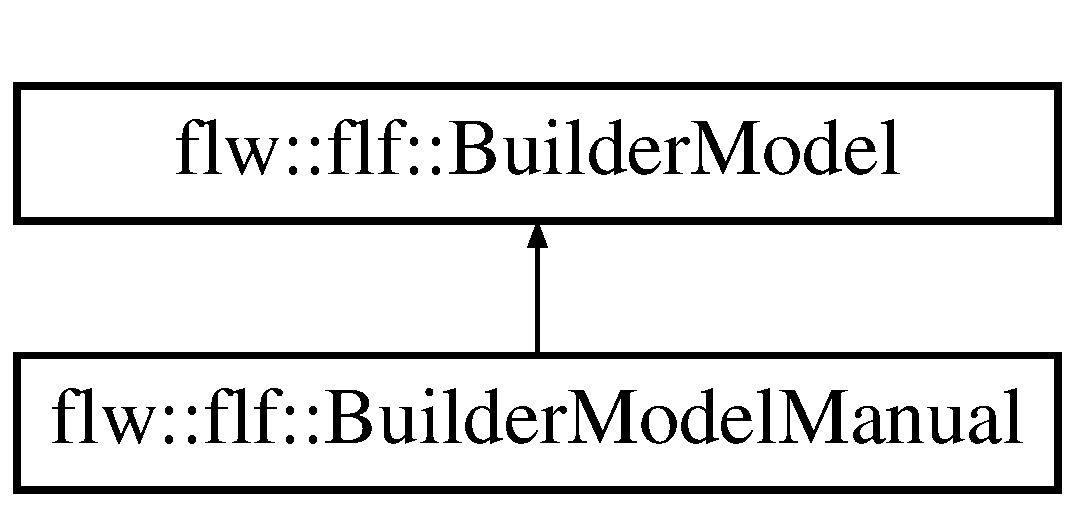
\includegraphics[height=2.000000cm]{classflw_1_1flf_1_1BuilderModelManual}
\end{center}
\end{figure}
\subsection*{Public Member Functions}
\begin{DoxyCompactItemize}
\item 
{\bfseries Builder\+Model\+Manual} (\hyperlink{classflw_1_1Engine}{Engine} $\ast$engine, std\+::string model\+Path=\char`\"{}\char`\"{}, \hyperlink{classflw_1_1flc_1_1Program}{flc\+::\+Program} $\ast$program=nullptr, \hyperlink{classflw_1_1flc_1_1Texture2D}{flc\+::\+Texture2D} $\ast$diffuse\+Map=nullptr, \hyperlink{classflw_1_1flc_1_1Texture2D}{flc\+::\+Texture2D} $\ast$normal\+Map=nullptr, \hyperlink{classflw_1_1flc_1_1Texture2D}{flc\+::\+Texture2D} $\ast$specular\+Map=nullptr, \hyperlink{classflw_1_1flf_1_1Material}{Material} material=\hyperlink{classflw_1_1flf_1_1Material}{Material}())\hypertarget{classflw_1_1flf_1_1BuilderModelManual_abb0c94af4b0f544fcde71ce11129fe58}{}\label{classflw_1_1flf_1_1BuilderModelManual_abb0c94af4b0f544fcde71ce11129fe58}

\item 
\hyperlink{classflw_1_1flf_1_1BuilderModelManual}{Builder\+Model\+Manual} \& {\bfseries set\+Diffuse\+Map\+Texture} (\hyperlink{classflw_1_1flc_1_1Texture2D}{flc\+::\+Texture2D} $\ast$texture)\hypertarget{classflw_1_1flf_1_1BuilderModelManual_ac147d3e5a9adcf0561d3831f44b592f3}{}\label{classflw_1_1flf_1_1BuilderModelManual_ac147d3e5a9adcf0561d3831f44b592f3}

\item 
\hyperlink{classflw_1_1flf_1_1BuilderModelManual}{Builder\+Model\+Manual} \& {\bfseries set\+Normal\+Map\+Texture} (\hyperlink{classflw_1_1flc_1_1Texture2D}{flc\+::\+Texture2D} $\ast$texture)\hypertarget{classflw_1_1flf_1_1BuilderModelManual_a472cbfc8bdb0bf654f761e21f6f19838}{}\label{classflw_1_1flf_1_1BuilderModelManual_a472cbfc8bdb0bf654f761e21f6f19838}

\item 
\hyperlink{classflw_1_1flf_1_1BuilderModelManual}{Builder\+Model\+Manual} \& {\bfseries set\+Specular\+Map\+Texture} (\hyperlink{classflw_1_1flc_1_1Texture2D}{flc\+::\+Texture2D} $\ast$texture)\hypertarget{classflw_1_1flf_1_1BuilderModelManual_acdd90ebb159ce182c9b970ca54371708}{}\label{classflw_1_1flf_1_1BuilderModelManual_acdd90ebb159ce182c9b970ca54371708}

\item 
\hyperlink{classflw_1_1flf_1_1BuilderModelManual}{Builder\+Model\+Manual} \& {\bfseries set\+Material} (const \hyperlink{classflw_1_1flf_1_1Material}{Material} \&material)\hypertarget{classflw_1_1flf_1_1BuilderModelManual_a3b3abbd5aca8f472306aaa8f195468ff}{}\label{classflw_1_1flf_1_1BuilderModelManual_a3b3abbd5aca8f472306aaa8f195468ff}

\item 
pu\+Model {\bfseries build} ()\hypertarget{classflw_1_1flf_1_1BuilderModelManual_a439cfce3c4cef0ae98ac15be6e40e710}{}\label{classflw_1_1flf_1_1BuilderModelManual_a439cfce3c4cef0ae98ac15be6e40e710}

\end{DoxyCompactItemize}
\subsection*{Additional Inherited Members}


\subsection{Detailed Description}
\hyperlink{classflw_1_1flf_1_1BuilderModel}{Builder\+Model} which builds the model from textures and material fillwave objects. 

The documentation for this class was generated from the following file\+:\begin{DoxyCompactItemize}
\item 
/home/filip/\+Projects/fillwave/inc/fillwave/models/builders/Builder\+Model\+Manual.\+h\end{DoxyCompactItemize}

\hypertarget{classflw_1_1flf_1_1Button}{}\section{flw\+:\+:flf\+:\+:Button Class Reference}
\label{classflw_1_1flf_1_1Button}\index{flw\+::flf\+::\+Button@{flw\+::flf\+::\+Button}}


Pickable hud node.  




{\ttfamily \#include $<$Button.\+h$>$}

Inheritance diagram for flw\+:\+:flf\+:\+:Button\+:\begin{figure}[H]
\begin{center}
\leavevmode
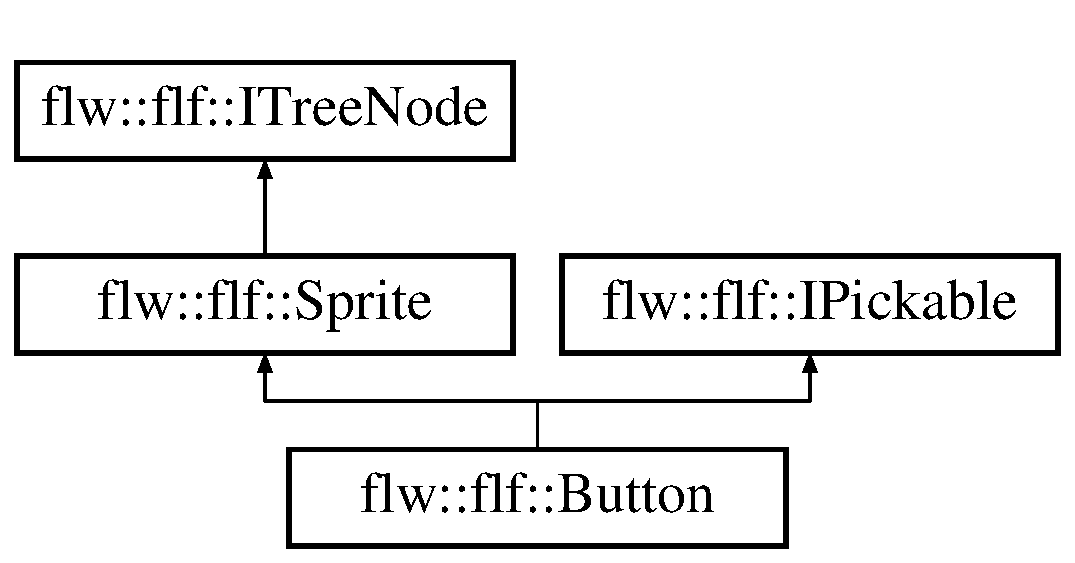
\includegraphics[height=3.000000cm]{classflw_1_1flf_1_1Button}
\end{center}
\end{figure}
\subsection*{Public Member Functions}
\begin{DoxyCompactItemize}
\item 
\mbox{\Hypertarget{classflw_1_1flf_1_1Button_ad3ae337aac8f1db876ac67decefac587}\label{classflw_1_1flf_1_1Button_ad3ae337aac8f1db876ac67decefac587}} 
{\bfseries Button} (\hyperlink{classflw_1_1Engine}{Engine} $\ast$engine, \hyperlink{classflw_1_1flc_1_1Texture2D}{flc\+::\+Texture2D} $\ast$texture, glm\+::vec2 position, glm\+::vec2 scale)
\item 
\mbox{\Hypertarget{classflw_1_1flf_1_1Button_a719b2df023e75d1706adcb83327fb94f}\label{classflw_1_1flf_1_1Button_a719b2df023e75d1706adcb83327fb94f}} 
void {\bfseries pick} (glm\+::vec3 color) override
\item 
\mbox{\Hypertarget{classflw_1_1flf_1_1Button_a70c6c0ad26ee8b953eaf7a4b8c477e42}\label{classflw_1_1flf_1_1Button_a70c6c0ad26ee8b953eaf7a4b8c477e42}} 
void {\bfseries unpick} () override
\item 
\mbox{\Hypertarget{classflw_1_1flf_1_1Button_a8ed9587ee4157b9b5c148f81e63b1a51}\label{classflw_1_1flf_1_1Button_a8ed9587ee4157b9b5c148f81e63b1a51}} 
void {\bfseries on\+Picked} () override
\item 
\mbox{\Hypertarget{classflw_1_1flf_1_1Button_aaf3a95201ffbd05d132cacd70fddb0c5}\label{classflw_1_1flf_1_1Button_aaf3a95201ffbd05d132cacd70fddb0c5}} 
void {\bfseries on\+Unpicked} () override
\end{DoxyCompactItemize}
\subsection*{Additional Inherited Members}


\subsection{Detailed Description}
Pickable hud node. 

The documentation for this class was generated from the following file\+:\begin{DoxyCompactItemize}
\item 
/home/filip/projects/fillwave/inc/fillwave/hud/Button.\+h\end{DoxyCompactItemize}

\hypertarget{classflw_1_1flf_1_1Callback}{}\section{flw\+:\+:flf\+:\+:Callback Class Reference}
\label{classflw_1_1flf_1_1Callback}\index{flw\+::flf\+::\+Callback@{flw\+::flf\+::\+Callback}}


Base for all callbacks.  




{\ttfamily \#include $<$Callback.\+h$>$}

Inheritance diagram for flw\+:\+:flf\+:\+:Callback\+:\begin{figure}[H]
\begin{center}
\leavevmode
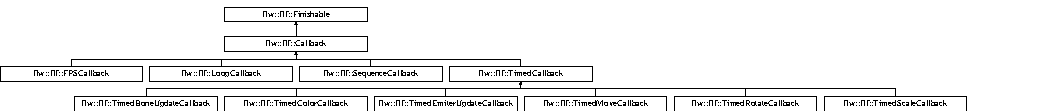
\includegraphics[height=1.488372cm]{classflw_1_1flf_1_1Callback}
\end{center}
\end{figure}
\subsection*{Public Member Functions}
\begin{DoxyCompactItemize}
\item 
{\bfseries Callback} (e\+Event\+Type event\+Type, float time\+To\+Finish=F\+I\+L\+L\+W\+A\+V\+E\+\_\+\+E\+N\+D\+L\+E\+SS)\hypertarget{classflw_1_1flf_1_1Callback_a45c89125621559a762cb8db7daeda563}{}\label{classflw_1_1flf_1_1Callback_a45c89125621559a762cb8db7daeda563}

\item 
virtual void {\bfseries perform} (\hyperlink{classflw_1_1flf_1_1EventType}{Event\+Type} \&event)=0\hypertarget{classflw_1_1flf_1_1Callback_affe144f7a3ce0dc7c2179885cc09bef4}{}\label{classflw_1_1flf_1_1Callback_affe144f7a3ce0dc7c2179885cc09bef4}

\item 
bool {\bfseries is\+Enabled} ()\hypertarget{classflw_1_1flf_1_1Callback_ae2b84ec364130d0f67742977dc7ae12e}{}\label{classflw_1_1flf_1_1Callback_ae2b84ec364130d0f67742977dc7ae12e}

\item 
void {\bfseries enable} ()\hypertarget{classflw_1_1flf_1_1Callback_a554532ba63957be6ac732c9c22b9fb9e}{}\label{classflw_1_1flf_1_1Callback_a554532ba63957be6ac732c9c22b9fb9e}

\item 
void {\bfseries disable} ()\hypertarget{classflw_1_1flf_1_1Callback_aece7ca52d68e153a2f6e30e780887004}{}\label{classflw_1_1flf_1_1Callback_aece7ca52d68e153a2f6e30e780887004}

\item 
e\+Event\+Type {\bfseries get\+Event\+Type} ()\hypertarget{classflw_1_1flf_1_1Callback_a806ac8cee59307bb901866bdc82edd79}{}\label{classflw_1_1flf_1_1Callback_a806ac8cee59307bb901866bdc82edd79}

\end{DoxyCompactItemize}
\subsection*{Static Public Member Functions}
\begin{DoxyCompactItemize}
\item 
{\footnotesize template$<$class T $>$ }\\static void {\bfseries handle\+Event} (std\+::vector$<$ T $>$ \&callbacks, \hyperlink{classflw_1_1flf_1_1EventType}{Event\+Type} \&event)\hypertarget{classflw_1_1flf_1_1Callback_a33d6db4add745c812829d6f4fb7f44f6}{}\label{classflw_1_1flf_1_1Callback_a33d6db4add745c812829d6f4fb7f44f6}

\end{DoxyCompactItemize}
\subsection*{Protected Attributes}
\begin{DoxyCompactItemize}
\item 
bool {\bfseries m\+Enabled}\hypertarget{classflw_1_1flf_1_1Callback_a9b9c7d9c864288b467a6404551a5d82a}{}\label{classflw_1_1flf_1_1Callback_a9b9c7d9c864288b467a6404551a5d82a}

\item 
e\+Event\+Type {\bfseries m\+Event\+Type}\hypertarget{classflw_1_1flf_1_1Callback_a8902c09a9bb26ccb04ef3e9b4e598938}{}\label{classflw_1_1flf_1_1Callback_a8902c09a9bb26ccb04ef3e9b4e598938}

\end{DoxyCompactItemize}


\subsection{Detailed Description}
Base for all callbacks. 

The documentation for this class was generated from the following file\+:\begin{DoxyCompactItemize}
\item 
/home/filip/\+Projects/fillwave/inc/fillwave/actions/callbacks/Callback.\+h\end{DoxyCompactItemize}

\hypertarget{classflw_1_1flf_1_1CameraNull}{}\section{flw\+:\+:flf\+:\+:Camera\+Null Class Reference}
\label{classflw_1_1flf_1_1CameraNull}\index{flw\+::flf\+::\+Camera\+Null@{flw\+::flf\+::\+Camera\+Null}}


Not used. Camera for which both projection and view matrices are always identities.  




{\ttfamily \#include $<$Camera\+Null.\+h$>$}

Inheritance diagram for flw\+:\+:flf\+:\+:Camera\+Null\+:\begin{figure}[H]
\begin{center}
\leavevmode
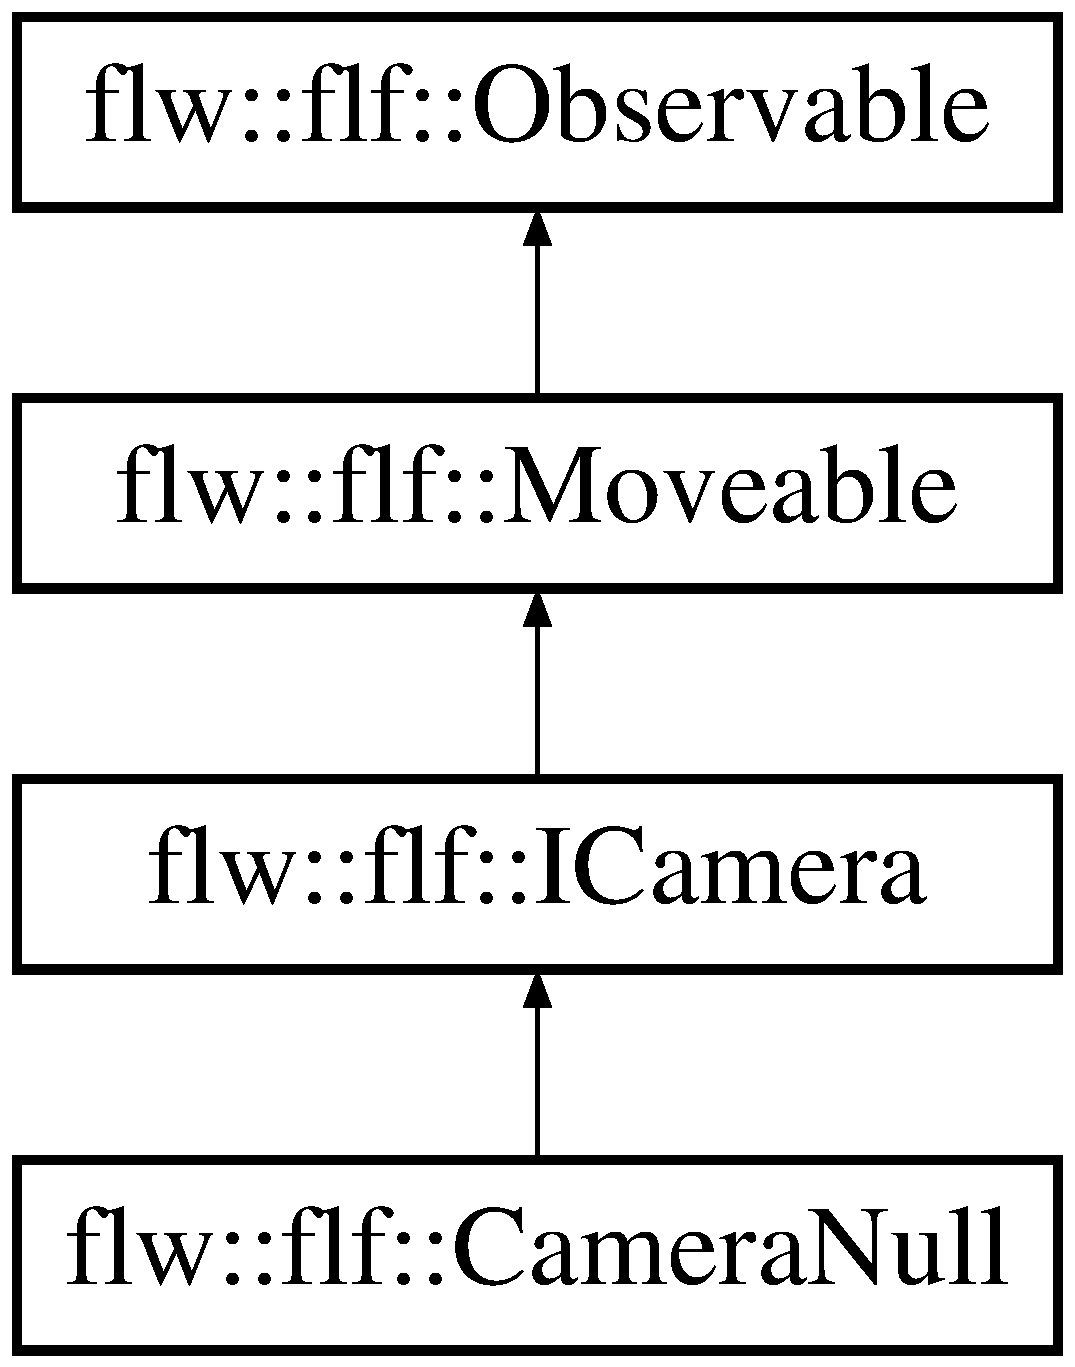
\includegraphics[height=4.000000cm]{classflw_1_1flf_1_1CameraNull}
\end{center}
\end{figure}
\subsection*{Public Member Functions}
\begin{DoxyCompactItemize}
\item 
\mbox{\Hypertarget{classflw_1_1flf_1_1CameraNull_ae8a26e5e560067bd9a84387a863d38f5}\label{classflw_1_1flf_1_1CameraNull_ae8a26e5e560067bd9a84387a863d38f5}} 
void {\bfseries update\+Projection} ()
\item 
\mbox{\Hypertarget{classflw_1_1flf_1_1CameraNull_a6ccddc568aba10bb69c05dadf8b3c89a}\label{classflw_1_1flf_1_1CameraNull_a6ccddc568aba10bb69c05dadf8b3c89a}} 
G\+Lfloat {\bfseries get\+Projection\+Near\+Plane} ()
\item 
\mbox{\Hypertarget{classflw_1_1flf_1_1CameraNull_a09741d600721440c3330d6404c2874d7}\label{classflw_1_1flf_1_1CameraNull_a09741d600721440c3330d6404c2874d7}} 
G\+Lfloat {\bfseries get\+Projection\+Far\+Plane} ()
\end{DoxyCompactItemize}
\subsection*{Additional Inherited Members}


\subsection{Detailed Description}
Not used. Camera for which both projection and view matrices are always identities. 

The documentation for this class was generated from the following file\+:\begin{DoxyCompactItemize}
\item 
/home/filip/projects/fillwave/inc/fillwave/space/Camera\+Null.\+h\end{DoxyCompactItemize}

\hypertarget{classflw_1_1flf_1_1CameraOrthographic}{}\section{flw\+:\+:flf\+:\+:Camera\+Orthographic Class Reference}
\label{classflw_1_1flf_1_1CameraOrthographic}\index{flw\+::flf\+::\+Camera\+Orthographic@{flw\+::flf\+::\+Camera\+Orthographic}}


Camera with Orthographic projection.  




{\ttfamily \#include $<$Camera\+Orthographic.\+h$>$}

Inheritance diagram for flw\+:\+:flf\+:\+:Camera\+Orthographic\+:\begin{figure}[H]
\begin{center}
\leavevmode
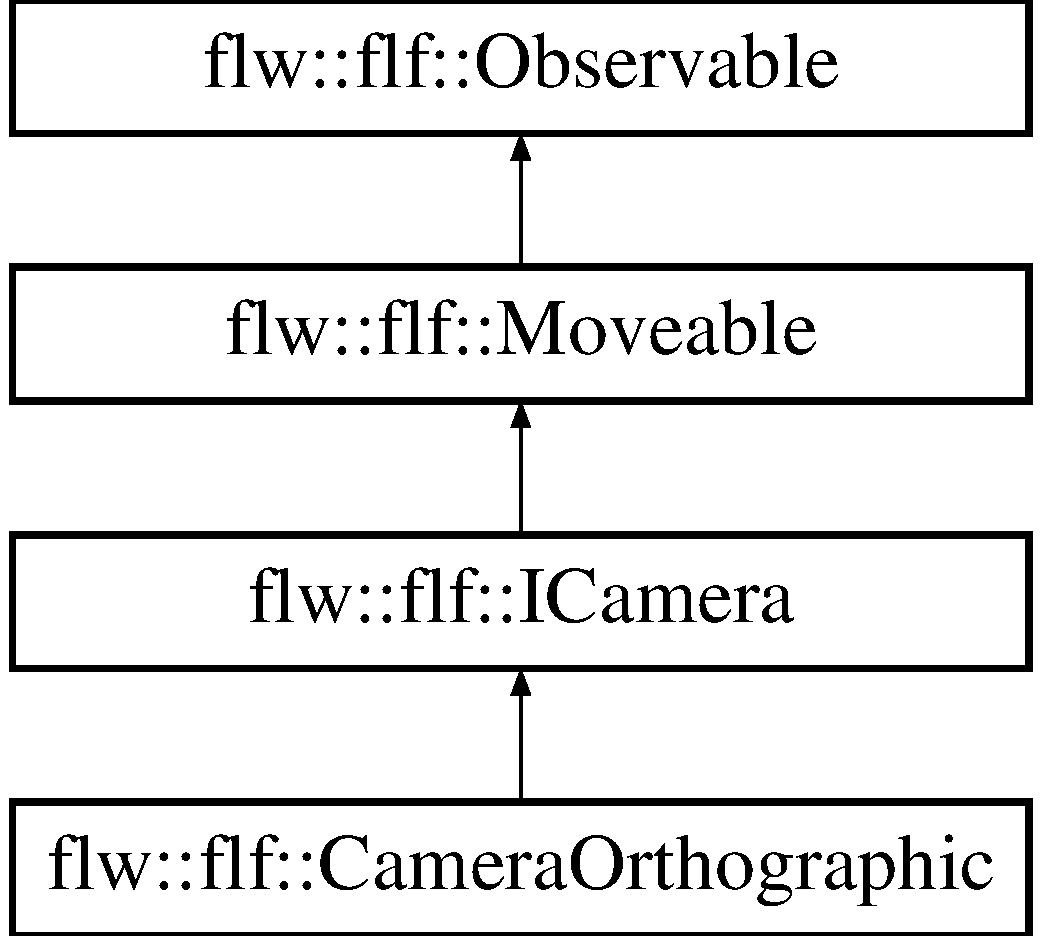
\includegraphics[height=4.000000cm]{classflw_1_1flf_1_1CameraOrthographic}
\end{center}
\end{figure}
\subsection*{Public Member Functions}
\begin{DoxyCompactItemize}
\item 
\mbox{\Hypertarget{classflw_1_1flf_1_1CameraOrthographic_af3256954755427e7d30080e4ddbc8bf2}\label{classflw_1_1flf_1_1CameraOrthographic_af3256954755427e7d30080e4ddbc8bf2}} 
{\bfseries Camera\+Orthographic} (glm\+::vec3 position, glm\+::quat rotation, G\+Lfloat left, G\+Lfloat right, G\+Lfloat bottom, G\+Lfloat top, G\+Lfloat near, G\+Lfloat far)
\item 
\mbox{\Hypertarget{classflw_1_1flf_1_1CameraOrthographic_a08256bc028355b465f23750e93718100}\label{classflw_1_1flf_1_1CameraOrthographic_a08256bc028355b465f23750e93718100}} 
void {\bfseries update\+Projection} ()
\item 
\mbox{\Hypertarget{classflw_1_1flf_1_1CameraOrthographic_ab3af2aed92db2745649c2af0fab6c277}\label{classflw_1_1flf_1_1CameraOrthographic_ab3af2aed92db2745649c2af0fab6c277}} 
G\+Lfloat {\bfseries get\+Projection\+Near\+Plane} ()
\item 
\mbox{\Hypertarget{classflw_1_1flf_1_1CameraOrthographic_ac1dde1e4ba781656d215348806844837}\label{classflw_1_1flf_1_1CameraOrthographic_ac1dde1e4ba781656d215348806844837}} 
G\+Lfloat {\bfseries get\+Projection\+Far\+Plane} ()
\end{DoxyCompactItemize}
\subsection*{Additional Inherited Members}


\subsection{Detailed Description}
Camera with Orthographic projection. 

The documentation for this class was generated from the following file\+:\begin{DoxyCompactItemize}
\item 
/home/filip/projects/fillwave/inc/fillwave/space/Camera\+Orthographic.\+h\end{DoxyCompactItemize}

\hypertarget{classflw_1_1flf_1_1CameraPerspective}{}\section{flw\+:\+:flf\+:\+:Camera\+Perspective Class Reference}
\label{classflw_1_1flf_1_1CameraPerspective}\index{flw\+::flf\+::\+Camera\+Perspective@{flw\+::flf\+::\+Camera\+Perspective}}


Camera with perspective projection.  




{\ttfamily \#include $<$Camera\+Perspective.\+h$>$}

Inheritance diagram for flw\+:\+:flf\+:\+:Camera\+Perspective\+:\begin{figure}[H]
\begin{center}
\leavevmode
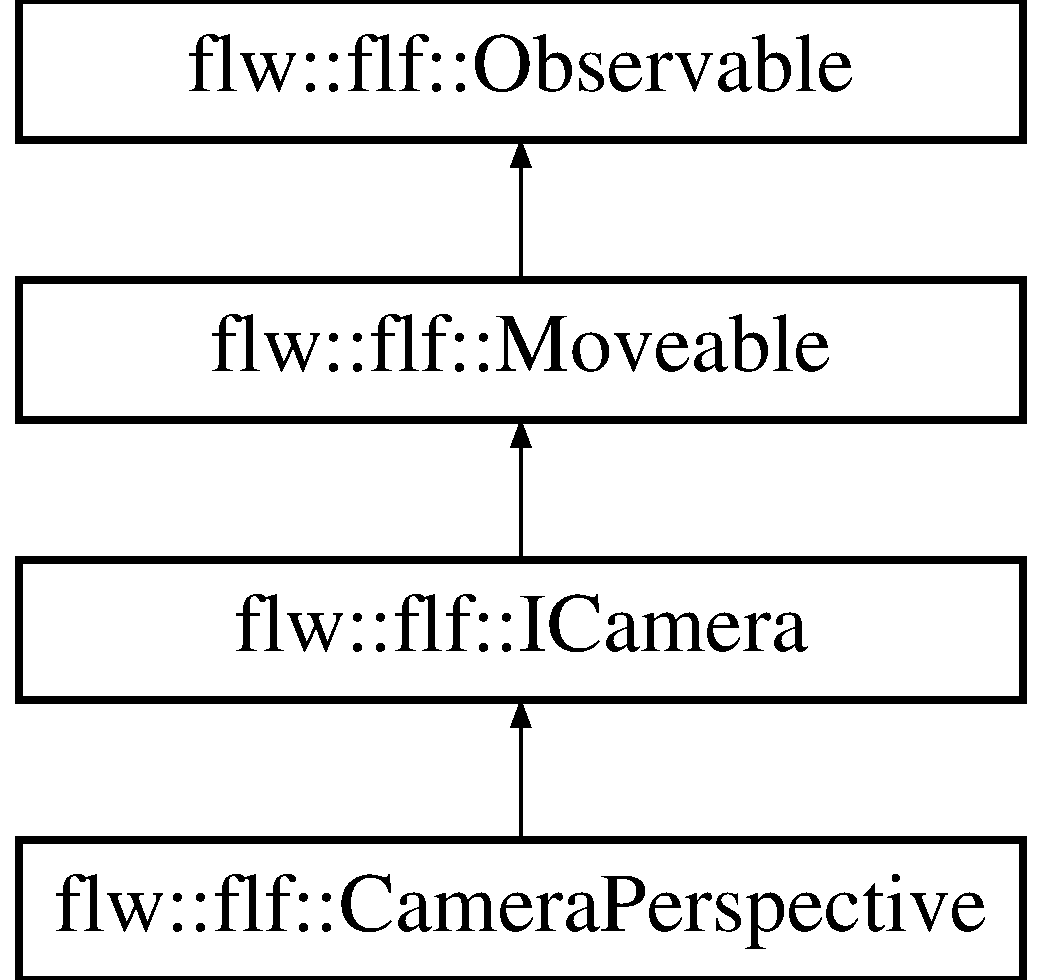
\includegraphics[height=4.000000cm]{classflw_1_1flf_1_1CameraPerspective}
\end{center}
\end{figure}
\subsection*{Public Member Functions}
\begin{DoxyCompactItemize}
\item 
{\bfseries Camera\+Perspective} (glm\+::vec3 position, glm\+::quat rotation, G\+Lfloat fovy=glm\+::radians(90.\+0f), G\+Lfloat aspect\+Ratio=1.\+0f, G\+Lfloat near\+Plane=0.\+01f, G\+Lfloat far\+Plane=100.\+0f)\hypertarget{classflw_1_1flf_1_1CameraPerspective_a379b92a93d9f8466d1d3e79a90465fa7}{}\label{classflw_1_1flf_1_1CameraPerspective_a379b92a93d9f8466d1d3e79a90465fa7}

\item 
G\+Lfloat {\bfseries get\+Projection\+Fovy} ()\hypertarget{classflw_1_1flf_1_1CameraPerspective_a0d38106602938a2b5b03a6db214ebcc0}{}\label{classflw_1_1flf_1_1CameraPerspective_a0d38106602938a2b5b03a6db214ebcc0}

\item 
G\+Lfloat {\bfseries get\+Projection\+Aspect\+Ratio} ()\hypertarget{classflw_1_1flf_1_1CameraPerspective_af49555679eb7d5a063643e30461d77ea}{}\label{classflw_1_1flf_1_1CameraPerspective_af49555679eb7d5a063643e30461d77ea}

\item 
G\+Lfloat {\bfseries get\+Projection\+Near\+Plane} ()\hypertarget{classflw_1_1flf_1_1CameraPerspective_ada21a63b8ead93a93e3de416036d08b8}{}\label{classflw_1_1flf_1_1CameraPerspective_ada21a63b8ead93a93e3de416036d08b8}

\item 
G\+Lfloat {\bfseries get\+Projection\+Far\+Plane} ()\hypertarget{classflw_1_1flf_1_1CameraPerspective_a0b19db2aaa3b7bb44bfe0b204ef341f9}{}\label{classflw_1_1flf_1_1CameraPerspective_a0b19db2aaa3b7bb44bfe0b204ef341f9}

\item 
void {\bfseries set\+Projection\+Fovy} (G\+Lfloat fovy)\hypertarget{classflw_1_1flf_1_1CameraPerspective_a68c18d3c8ccd52fc48db96973e45b525}{}\label{classflw_1_1flf_1_1CameraPerspective_a68c18d3c8ccd52fc48db96973e45b525}

\item 
void {\bfseries set\+Projection\+Aspect\+Ratio} (G\+Lfloat aspect)\hypertarget{classflw_1_1flf_1_1CameraPerspective_a19b54c2d676effb8e7b1986e4ddd5d7c}{}\label{classflw_1_1flf_1_1CameraPerspective_a19b54c2d676effb8e7b1986e4ddd5d7c}

\item 
void {\bfseries set\+Projection\+Near\+Plane} (G\+Lfloat near\+Plane)\hypertarget{classflw_1_1flf_1_1CameraPerspective_a7e7d41e82ede68c179646ab96ae93c1c}{}\label{classflw_1_1flf_1_1CameraPerspective_a7e7d41e82ede68c179646ab96ae93c1c}

\item 
void {\bfseries set\+Projection\+Far\+Plane} (G\+Lfloat far\+Plane)\hypertarget{classflw_1_1flf_1_1CameraPerspective_aed83834404ba2025de37207ab2453850}{}\label{classflw_1_1flf_1_1CameraPerspective_aed83834404ba2025de37207ab2453850}

\item 
void {\bfseries update\+Projection} ()\hypertarget{classflw_1_1flf_1_1CameraPerspective_aca94b0f08121b76fe51d99d6685de097}{}\label{classflw_1_1flf_1_1CameraPerspective_aca94b0f08121b76fe51d99d6685de097}

\end{DoxyCompactItemize}
\subsection*{Additional Inherited Members}


\subsection{Detailed Description}
Camera with perspective projection. 

The documentation for this class was generated from the following file\+:\begin{DoxyCompactItemize}
\item 
/home/filip/\+Projects/fillwave/inc/fillwave/space/Camera\+Perspective.\+h\end{DoxyCompactItemize}

\hypertarget{classflw_1_1flf_1_1Channel}{}\section{flw\+:\+:flf\+:\+:Channel Class Reference}
\label{classflw_1_1flf_1_1Channel}\index{flw\+::flf\+::\+Channel@{flw\+::flf\+::\+Channel}}


wrapper to assimp ai\+Node\+Anim$\ast$  




{\ttfamily \#include $<$Channel.\+h$>$}

\subsection*{Public Member Functions}
\begin{DoxyCompactItemize}
\item 
{\bfseries Channel} (ai\+Node\+Anim $\ast$assimp\+Channel)\hypertarget{classflw_1_1flf_1_1Channel_a68388e17e6a802feb500298f6ebae8b7}{}\label{classflw_1_1flf_1_1Channel_a68388e17e6a802feb500298f6ebae8b7}

\end{DoxyCompactItemize}
\subsection*{Public Attributes}
\begin{DoxyCompactItemize}
\item 
std\+::string {\bfseries m\+Affected\+Node\+Name}\hypertarget{classflw_1_1flf_1_1Channel_a2be55ddd58a96c0e5f75e27ee5ece8c0}{}\label{classflw_1_1flf_1_1Channel_a2be55ddd58a96c0e5f75e27ee5ece8c0}

\item 
std\+::vector$<$ \hyperlink{classflw_1_1flf_1_1Key}{Key}$<$ glm\+::vec3 $>$ $>$ {\bfseries m\+Keys\+Translation}\hypertarget{classflw_1_1flf_1_1Channel_a5c976df532a44512d02002054c6fc7db}{}\label{classflw_1_1flf_1_1Channel_a5c976df532a44512d02002054c6fc7db}

\item 
std\+::vector$<$ \hyperlink{classflw_1_1flf_1_1Key}{Key}$<$ glm\+::quat $>$ $>$ {\bfseries m\+Keys\+Rotation}\hypertarget{classflw_1_1flf_1_1Channel_a878c9d16a562846be380bf1539da775b}{}\label{classflw_1_1flf_1_1Channel_a878c9d16a562846be380bf1539da775b}

\item 
std\+::vector$<$ \hyperlink{classflw_1_1flf_1_1Key}{Key}$<$ glm\+::vec3 $>$ $>$ {\bfseries m\+Keys\+Scaling}\hypertarget{classflw_1_1flf_1_1Channel_a85e59bc7ef520eab7656af136bc9d43c}{}\label{classflw_1_1flf_1_1Channel_a85e59bc7ef520eab7656af136bc9d43c}

\end{DoxyCompactItemize}


\subsection{Detailed Description}
wrapper to assimp ai\+Node\+Anim$\ast$ 

The documentation for this class was generated from the following file\+:\begin{DoxyCompactItemize}
\item 
/home/filip/\+Projects/fillwave/inc/fillwave/models/animations/Channel.\+h\end{DoxyCompactItemize}

\hypertarget{classflw_1_1flf_1_1CharacterEvent}{}\section{flw\+:\+:flf\+:\+:Character\+Event Struct Reference}
\label{classflw_1_1flf_1_1CharacterEvent}\index{flw\+::flf\+::\+Character\+Event@{flw\+::flf\+::\+Character\+Event}}


Event introduced when the key is pressed.  




{\ttfamily \#include $<$Character\+T\+Event.\+h$>$}

Inheritance diagram for flw\+:\+:flf\+:\+:Character\+Event\+:\begin{figure}[H]
\begin{center}
\leavevmode
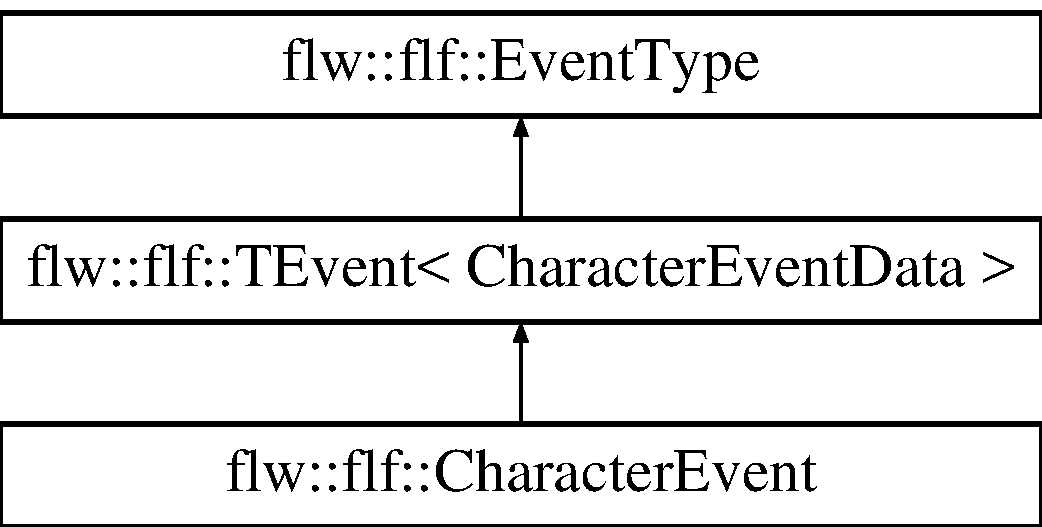
\includegraphics[height=3.000000cm]{classflw_1_1flf_1_1CharacterEvent}
\end{center}
\end{figure}
\subsection*{Public Member Functions}
\begin{DoxyCompactItemize}
\item 
{\bfseries Character\+Event} (\hyperlink{structflw_1_1flf_1_1CharacterEventData}{Character\+Event\+Data} \&data)\hypertarget{classflw_1_1flf_1_1CharacterEvent_a508be13f56ac32c57af8db79860aead4}{}\label{classflw_1_1flf_1_1CharacterEvent_a508be13f56ac32c57af8db79860aead4}

\end{DoxyCompactItemize}
\subsection*{Additional Inherited Members}


\subsection{Detailed Description}
Event introduced when the key is pressed. 

The documentation for this struct was generated from the following file\+:\begin{DoxyCompactItemize}
\item 
/home/filip/\+Projects/fillwave/inc/fillwave/actions/events/Character\+T\+Event.\+h\end{DoxyCompactItemize}

\hypertarget{structflw_1_1flf_1_1CharacterEventData}{}\section{flw\+:\+:flf\+:\+:Character\+Event\+Data Struct Reference}
\label{structflw_1_1flf_1_1CharacterEventData}\index{flw\+::flf\+::\+Character\+Event\+Data@{flw\+::flf\+::\+Character\+Event\+Data}}


Event data structure to store the character.  




{\ttfamily \#include $<$Character\+T\+Event.\+h$>$}

\subsection*{Public Attributes}
\begin{DoxyCompactItemize}
\item 
unsigned int {\bfseries character}\hypertarget{structflw_1_1flf_1_1CharacterEventData_a66078927332efbd386b6f0a4fb767d38}{}\label{structflw_1_1flf_1_1CharacterEventData_a66078927332efbd386b6f0a4fb767d38}

\item 
const e\+Event\+Type {\bfseries type} = e\+Event\+Type\+::e\+Character\hypertarget{structflw_1_1flf_1_1CharacterEventData_a65d408be95581d3384af0c5bd014c120}{}\label{structflw_1_1flf_1_1CharacterEventData_a65d408be95581d3384af0c5bd014c120}

\end{DoxyCompactItemize}


\subsection{Detailed Description}
Event data structure to store the character. 

The documentation for this struct was generated from the following file\+:\begin{DoxyCompactItemize}
\item 
/home/filip/\+Projects/fillwave/inc/fillwave/actions/events/Character\+T\+Event.\+h\end{DoxyCompactItemize}

\hypertarget{classflw_1_1flf_1_1CharacterModsEvent}{}\section{flw\+:\+:flf\+:\+:Character\+Mods\+Event Struct Reference}
\label{classflw_1_1flf_1_1CharacterModsEvent}\index{flw\+::flf\+::\+Character\+Mods\+Event@{flw\+::flf\+::\+Character\+Mods\+Event}}


Event introduced when the key is pressed.  




{\ttfamily \#include $<$Character\+Mods\+T\+Event.\+h$>$}

Inheritance diagram for flw\+:\+:flf\+:\+:Character\+Mods\+Event\+:\begin{figure}[H]
\begin{center}
\leavevmode
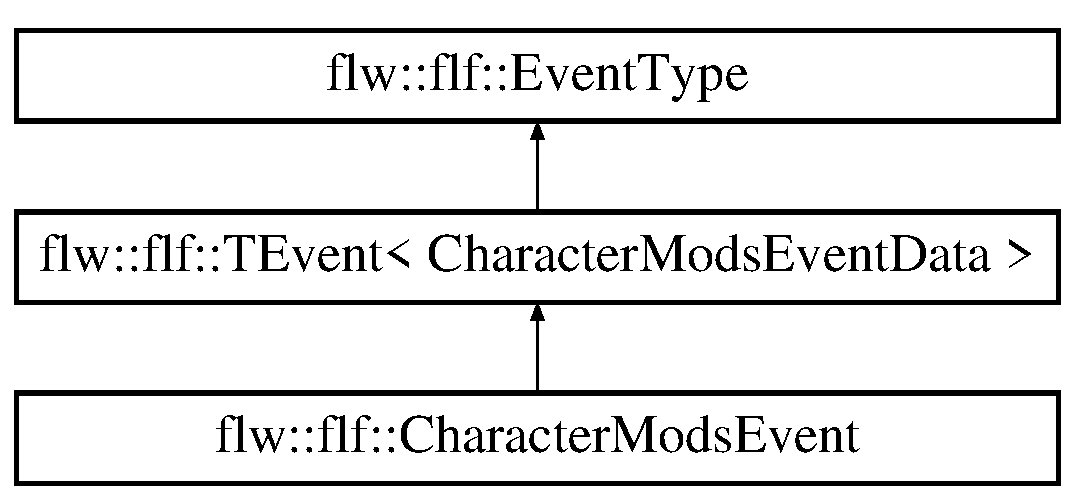
\includegraphics[height=3.000000cm]{classflw_1_1flf_1_1CharacterModsEvent}
\end{center}
\end{figure}
\subsection*{Public Member Functions}
\begin{DoxyCompactItemize}
\item 
{\bfseries Character\+Mods\+Event} (\hyperlink{structflw_1_1flf_1_1CharacterModsEventData}{Character\+Mods\+Event\+Data} \&data)\hypertarget{classflw_1_1flf_1_1CharacterModsEvent_a828d334f22e00b4435f9a5be0b705702}{}\label{classflw_1_1flf_1_1CharacterModsEvent_a828d334f22e00b4435f9a5be0b705702}

\end{DoxyCompactItemize}
\subsection*{Additional Inherited Members}


\subsection{Detailed Description}
Event introduced when the key is pressed. 

The documentation for this struct was generated from the following file\+:\begin{DoxyCompactItemize}
\item 
/home/filip/\+Projects/fillwave/inc/fillwave/actions/events/Character\+Mods\+T\+Event.\+h\end{DoxyCompactItemize}

\hypertarget{structflw_1_1flf_1_1CharacterModsEventData}{}\section{flw\+:\+:flf\+:\+:Character\+Mods\+Event\+Data Struct Reference}
\label{structflw_1_1flf_1_1CharacterModsEventData}\index{flw\+::flf\+::\+Character\+Mods\+Event\+Data@{flw\+::flf\+::\+Character\+Mods\+Event\+Data}}


Event data structure to store the character together with modifier keys.  




{\ttfamily \#include $<$Character\+Mods\+T\+Event.\+h$>$}

\subsection*{Public Attributes}
\begin{DoxyCompactItemize}
\item 
unsigned int {\bfseries character}\hypertarget{structflw_1_1flf_1_1CharacterModsEventData_a4796fb81b9ac68e43b4d2bf2385f1470}{}\label{structflw_1_1flf_1_1CharacterModsEventData_a4796fb81b9ac68e43b4d2bf2385f1470}

\item 
int {\bfseries modsifier\+Keys}\hypertarget{structflw_1_1flf_1_1CharacterModsEventData_ab1383f98fa3c6243e4e12ea804b67c38}{}\label{structflw_1_1flf_1_1CharacterModsEventData_ab1383f98fa3c6243e4e12ea804b67c38}

\item 
const e\+Event\+Type {\bfseries type} = e\+Event\+Type\+::e\+Character\+Mods\hypertarget{structflw_1_1flf_1_1CharacterModsEventData_a2494e4b85d6da62484bedacd652ed6dd}{}\label{structflw_1_1flf_1_1CharacterModsEventData_a2494e4b85d6da62484bedacd652ed6dd}

\end{DoxyCompactItemize}


\subsection{Detailed Description}
Event data structure to store the character together with modifier keys. 

The documentation for this struct was generated from the following file\+:\begin{DoxyCompactItemize}
\item 
/home/filip/\+Projects/fillwave/inc/fillwave/actions/events/Character\+Mods\+T\+Event.\+h\end{DoxyCompactItemize}

\hypertarget{classflw_1_1flf_1_1ClockwiseDrawEffect}{}\section{flw\+:\+:flf\+:\+:Clockwise\+Draw\+Effect Class Reference}
\label{classflw_1_1flf_1_1ClockwiseDrawEffect}\index{flw\+::flf\+::\+Clockwise\+Draw\+Effect@{flw\+::flf\+::\+Clockwise\+Draw\+Effect}}


Effect to draw an opposite face of each mesh.  




{\ttfamily \#include $<$Clockwise\+Draw\+Effect.\+h$>$}

Inheritance diagram for flw\+:\+:flf\+:\+:Clockwise\+Draw\+Effect\+:\begin{figure}[H]
\begin{center}
\leavevmode
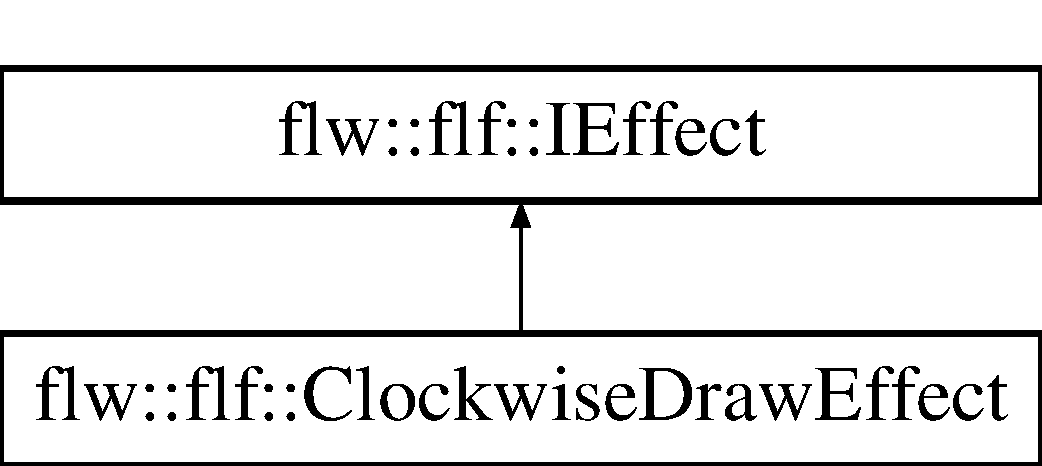
\includegraphics[height=2.000000cm]{classflw_1_1flf_1_1ClockwiseDrawEffect}
\end{center}
\end{figure}
\subsection*{Public Member Functions}
\begin{DoxyCompactItemize}
\item 
void \hyperlink{classflw_1_1flf_1_1ClockwiseDrawEffect_ab6a8333c2a80dbc56190b73f3d06264e}{pre\+Draw\+Action} (\hyperlink{classflw_1_1flc_1_1Program}{flc\+::\+Program} $\ast$program)
\begin{DoxyCompactList}\small\item\em virtual\+: defines action to be done just before the draw. \end{DoxyCompactList}\item 
void \hyperlink{classflw_1_1flf_1_1ClockwiseDrawEffect_a7ca5b12de498014fd1b7320fbe749e4e}{post\+Draw\+Action} (\hyperlink{classflw_1_1flc_1_1Program}{flc\+::\+Program} $\ast$program)
\begin{DoxyCompactList}\small\item\em virtual\+: defines action to be done just after the draw. \end{DoxyCompactList}\item 
void \hyperlink{classflw_1_1flf_1_1ClockwiseDrawEffect_a538235e072e91bfa16e185a535547679}{stop\+Action} (\hyperlink{classflw_1_1flc_1_1Program}{flc\+::\+Program} $\ast$program)
\begin{DoxyCompactList}\small\item\em virtual\+: defines action to be done when the effect is stopped. \end{DoxyCompactList}\item 
void \hyperlink{classflw_1_1flf_1_1ClockwiseDrawEffect_a5d6c2f7e723f845f615572721f79a5a8}{start\+Action} (\hyperlink{classflw_1_1flc_1_1Program}{flc\+::\+Program} $\ast$program)
\begin{DoxyCompactList}\small\item\em virtual\+: defines action to be done when the effect is started. \end{DoxyCompactList}\end{DoxyCompactItemize}


\subsection{Detailed Description}
Effect to draw an opposite face of each mesh. 

\subsection{Member Function Documentation}
\index{flw\+::flf\+::\+Clockwise\+Draw\+Effect@{flw\+::flf\+::\+Clockwise\+Draw\+Effect}!post\+Draw\+Action@{post\+Draw\+Action}}
\index{post\+Draw\+Action@{post\+Draw\+Action}!flw\+::flf\+::\+Clockwise\+Draw\+Effect@{flw\+::flf\+::\+Clockwise\+Draw\+Effect}}
\subsubsection[{\texorpdfstring{post\+Draw\+Action(flc\+::\+Program $\ast$program)}{postDrawAction(flc::Program *program)}}]{\setlength{\rightskip}{0pt plus 5cm}void flw\+::flf\+::\+Clockwise\+Draw\+Effect\+::post\+Draw\+Action (
\begin{DoxyParamCaption}
\item[{{\bf flc\+::\+Program} $\ast$}]{program}
\end{DoxyParamCaption}
)\hspace{0.3cm}{\ttfamily [virtual]}}\hypertarget{classflw_1_1flf_1_1ClockwiseDrawEffect_a7ca5b12de498014fd1b7320fbe749e4e}{}\label{classflw_1_1flf_1_1ClockwiseDrawEffect_a7ca5b12de498014fd1b7320fbe749e4e}


virtual\+: defines action to be done just after the draw. 

post\+Draw\+Action 

Implements \hyperlink{classflw_1_1flf_1_1IEffect_a6bb11d90e7e4da057ca398bd8c61208a}{flw\+::flf\+::\+I\+Effect}.

\index{flw\+::flf\+::\+Clockwise\+Draw\+Effect@{flw\+::flf\+::\+Clockwise\+Draw\+Effect}!pre\+Draw\+Action@{pre\+Draw\+Action}}
\index{pre\+Draw\+Action@{pre\+Draw\+Action}!flw\+::flf\+::\+Clockwise\+Draw\+Effect@{flw\+::flf\+::\+Clockwise\+Draw\+Effect}}
\subsubsection[{\texorpdfstring{pre\+Draw\+Action(flc\+::\+Program $\ast$program)}{preDrawAction(flc::Program *program)}}]{\setlength{\rightskip}{0pt plus 5cm}void flw\+::flf\+::\+Clockwise\+Draw\+Effect\+::pre\+Draw\+Action (
\begin{DoxyParamCaption}
\item[{{\bf flc\+::\+Program} $\ast$}]{program}
\end{DoxyParamCaption}
)\hspace{0.3cm}{\ttfamily [virtual]}}\hypertarget{classflw_1_1flf_1_1ClockwiseDrawEffect_ab6a8333c2a80dbc56190b73f3d06264e}{}\label{classflw_1_1flf_1_1ClockwiseDrawEffect_ab6a8333c2a80dbc56190b73f3d06264e}


virtual\+: defines action to be done just before the draw. 

pre\+Draw\+Action 

Implements \hyperlink{classflw_1_1flf_1_1IEffect_ae65eed21e40a226c7739d3c5dedd9e50}{flw\+::flf\+::\+I\+Effect}.

\index{flw\+::flf\+::\+Clockwise\+Draw\+Effect@{flw\+::flf\+::\+Clockwise\+Draw\+Effect}!start\+Action@{start\+Action}}
\index{start\+Action@{start\+Action}!flw\+::flf\+::\+Clockwise\+Draw\+Effect@{flw\+::flf\+::\+Clockwise\+Draw\+Effect}}
\subsubsection[{\texorpdfstring{start\+Action(flc\+::\+Program $\ast$program)}{startAction(flc::Program *program)}}]{\setlength{\rightskip}{0pt plus 5cm}void flw\+::flf\+::\+Clockwise\+Draw\+Effect\+::start\+Action (
\begin{DoxyParamCaption}
\item[{{\bf flc\+::\+Program} $\ast$}]{program}
\end{DoxyParamCaption}
)\hspace{0.3cm}{\ttfamily [virtual]}}\hypertarget{classflw_1_1flf_1_1ClockwiseDrawEffect_a5d6c2f7e723f845f615572721f79a5a8}{}\label{classflw_1_1flf_1_1ClockwiseDrawEffect_a5d6c2f7e723f845f615572721f79a5a8}


virtual\+: defines action to be done when the effect is started. 

start\+Action 

Implements \hyperlink{classflw_1_1flf_1_1IEffect_afc7cec9080d135ed264b08a90c7b94e9}{flw\+::flf\+::\+I\+Effect}.

\index{flw\+::flf\+::\+Clockwise\+Draw\+Effect@{flw\+::flf\+::\+Clockwise\+Draw\+Effect}!stop\+Action@{stop\+Action}}
\index{stop\+Action@{stop\+Action}!flw\+::flf\+::\+Clockwise\+Draw\+Effect@{flw\+::flf\+::\+Clockwise\+Draw\+Effect}}
\subsubsection[{\texorpdfstring{stop\+Action(flc\+::\+Program $\ast$program)}{stopAction(flc::Program *program)}}]{\setlength{\rightskip}{0pt plus 5cm}void flw\+::flf\+::\+Clockwise\+Draw\+Effect\+::stop\+Action (
\begin{DoxyParamCaption}
\item[{{\bf flc\+::\+Program} $\ast$}]{program}
\end{DoxyParamCaption}
)\hspace{0.3cm}{\ttfamily [virtual]}}\hypertarget{classflw_1_1flf_1_1ClockwiseDrawEffect_a538235e072e91bfa16e185a535547679}{}\label{classflw_1_1flf_1_1ClockwiseDrawEffect_a538235e072e91bfa16e185a535547679}


virtual\+: defines action to be done when the effect is stopped. 

stop\+Action 

Implements \hyperlink{classflw_1_1flf_1_1IEffect_a1a03eaf63a9d4edbd8764540d2d4133c}{flw\+::flf\+::\+I\+Effect}.



The documentation for this class was generated from the following file\+:\begin{DoxyCompactItemize}
\item 
/home/filip/\+Projects/fillwave/inc/fillwave/models/effects/Clockwise\+Draw\+Effect.\+h\end{DoxyCompactItemize}

\hypertarget{classflw_1_1flc_1_1ConditionalRender}{}\section{flw\+:\+:flc\+:\+:Conditional\+Render Class Reference}
\label{classflw_1_1flc_1_1ConditionalRender}\index{flw\+::flc\+::\+Conditional\+Render@{flw\+::flc\+::\+Conditional\+Render}}


Operation of rendering only meshes passing the occlusion test.  




{\ttfamily \#include $<$Conditional\+Render.\+h$>$}

\subsection*{Public Member Functions}
\begin{DoxyCompactItemize}
\item 
\hyperlink{classflw_1_1flc_1_1ConditionalRender_aaa7bf9c82c8631afea3e70fa164be287}{Conditional\+Render} (G\+Lenum mode)
\begin{DoxyCompactList}\small\item\em Specifies the conditional rendering pass mode. \end{DoxyCompactList}\item 
void {\bfseries begin} (G\+Luint querry\+ID) const \hypertarget{classflw_1_1flc_1_1ConditionalRender_ac7aaf6e2bdf618718a358f1cee679b5c}{}\label{classflw_1_1flc_1_1ConditionalRender_ac7aaf6e2bdf618718a358f1cee679b5c}

\item 
void {\bfseries end} () const \hypertarget{classflw_1_1flc_1_1ConditionalRender_a013c1c6f402634df4affb40abb3e75df}{}\label{classflw_1_1flc_1_1ConditionalRender_a013c1c6f402634df4affb40abb3e75df}

\end{DoxyCompactItemize}


\subsection{Detailed Description}
Operation of rendering only meshes passing the occlusion test. 

\subsection{Constructor \& Destructor Documentation}
\index{flw\+::flc\+::\+Conditional\+Render@{flw\+::flc\+::\+Conditional\+Render}!Conditional\+Render@{Conditional\+Render}}
\index{Conditional\+Render@{Conditional\+Render}!flw\+::flc\+::\+Conditional\+Render@{flw\+::flc\+::\+Conditional\+Render}}
\subsubsection[{\texorpdfstring{Conditional\+Render(\+G\+Lenum mode)}{ConditionalRender(GLenum mode)}}]{\setlength{\rightskip}{0pt plus 5cm}flw\+::flc\+::\+Conditional\+Render\+::\+Conditional\+Render (
\begin{DoxyParamCaption}
\item[{G\+Lenum}]{mode}
\end{DoxyParamCaption}
)}\hypertarget{classflw_1_1flc_1_1ConditionalRender_aaa7bf9c82c8631afea3e70fa164be287}{}\label{classflw_1_1flc_1_1ConditionalRender_aaa7bf9c82c8631afea3e70fa164be287}


Specifies the conditional rendering pass mode. 


\begin{DoxyParams}{Parameters}
{\em Possible} & modes\+: G\+L\+\_\+\+Q\+U\+E\+R\+Y\+\_\+\+W\+A\+IT, G\+L\+\_\+\+Q\+U\+E\+R\+Y\+\_\+\+N\+O\+\_\+\+W\+A\+IT, G\+L\+\_\+\+Q\+U\+E\+R\+Y\+\_\+\+B\+Y\+\_\+\+R\+E\+G\+I\+O\+N\+\_\+\+W\+A\+IT, G\+L\+\_\+\+Q\+U\+E\+R\+Y\+\_\+\+B\+Y\+\_\+\+R\+E\+G\+I\+O\+N\+\_\+\+N\+O\+\_\+\+W\+A\+IT, \\
\hline
\end{DoxyParams}


The documentation for this class was generated from the following file\+:\begin{DoxyCompactItemize}
\item 
/home/filip/\+Projects/fillwave/inc/fillwave/core/operations/Conditional\+Render.\+h\end{DoxyCompactItemize}

\hypertarget{structflw_1_1flf_1_1CullingBox}{}\section{flw\+:\+:flf\+:\+:Culling\+Box Class Reference}
\label{structflw_1_1flf_1_1CullingBox}\index{flw\+::flf\+::\+Culling\+Box@{flw\+::flf\+::\+Culling\+Box}}


Stores culling box parameters for Orthographic projection.  




{\ttfamily \#include $<$Camera\+Orthographic.\+h$>$}

\subsection*{Public Attributes}
\begin{DoxyCompactItemize}
\item 
G\+Lfloat {\bfseries m\+Projection\+Left}\hypertarget{structflw_1_1flf_1_1CullingBox_ac5c2e8a66f067c2df77d106ca3581dff}{}\label{structflw_1_1flf_1_1CullingBox_ac5c2e8a66f067c2df77d106ca3581dff}

\item 
G\+Lfloat {\bfseries m\+Projection\+Right}\hypertarget{structflw_1_1flf_1_1CullingBox_a4da4f46dd3c7db0917ad2d7cfb898969}{}\label{structflw_1_1flf_1_1CullingBox_a4da4f46dd3c7db0917ad2d7cfb898969}

\item 
G\+Lfloat {\bfseries m\+Projection\+Bottom}\hypertarget{structflw_1_1flf_1_1CullingBox_a023494058764b2e32487c74ca6f0ca5a}{}\label{structflw_1_1flf_1_1CullingBox_a023494058764b2e32487c74ca6f0ca5a}

\item 
G\+Lfloat {\bfseries m\+Projection\+Top}\hypertarget{structflw_1_1flf_1_1CullingBox_a00c8442039df52349d7270b380fa6107}{}\label{structflw_1_1flf_1_1CullingBox_a00c8442039df52349d7270b380fa6107}

\item 
G\+Lfloat {\bfseries m\+Projection\+Near}\hypertarget{structflw_1_1flf_1_1CullingBox_a83129de939fbe7d4dd1cb53d3d6a05ed}{}\label{structflw_1_1flf_1_1CullingBox_a83129de939fbe7d4dd1cb53d3d6a05ed}

\item 
G\+Lfloat {\bfseries m\+Projection\+Far}\hypertarget{structflw_1_1flf_1_1CullingBox_a23e77401e6e69cdc66985ae21ddf4251}{}\label{structflw_1_1flf_1_1CullingBox_a23e77401e6e69cdc66985ae21ddf4251}

\end{DoxyCompactItemize}


\subsection{Detailed Description}
Stores culling box parameters for Orthographic projection. 

The documentation for this class was generated from the following file\+:\begin{DoxyCompactItemize}
\item 
/home/filip/\+Projects/fillwave/inc/fillwave/space/Camera\+Orthographic.\+h\end{DoxyCompactItemize}

\hypertarget{classflw_1_1flf_1_1Cursor}{}\section{flw\+:\+:flf\+:\+:Cursor Class Reference}
\label{classflw_1_1flf_1_1Cursor}\index{flw\+::flf\+::\+Cursor@{flw\+::flf\+::\+Cursor}}


\hyperlink{classflw_1_1flf_1_1Impostor}{Impostor} to handle custom cursor instead of the standard one.  




{\ttfamily \#include $<$Cursor.\+h$>$}

Inheritance diagram for flw\+:\+:flf\+:\+:Cursor\+:\begin{figure}[H]
\begin{center}
\leavevmode
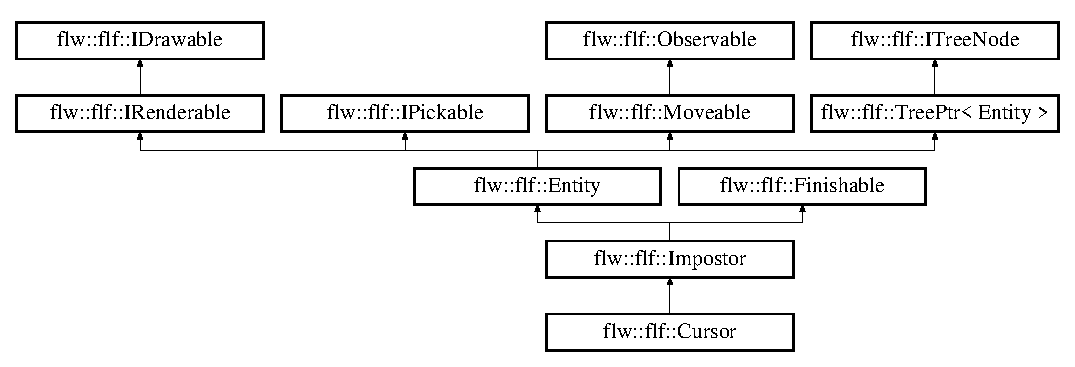
\includegraphics[height=4.487180cm]{classflw_1_1flf_1_1Cursor}
\end{center}
\end{figure}
\subsection*{Public Member Functions}
\begin{DoxyCompactItemize}
\item 
{\bfseries Cursor} (\hyperlink{classflw_1_1Engine}{Engine} $\ast$engine, \hyperlink{classflw_1_1flc_1_1Texture}{flc\+::\+Texture} $\ast$texture)\hypertarget{classflw_1_1flf_1_1Cursor_a339bd00cbcad4d867222ffedbbdce45e}{}\label{classflw_1_1flf_1_1Cursor_a339bd00cbcad4d867222ffedbbdce45e}

\item 
void {\bfseries move} (glm\+::vec2 position)\hypertarget{classflw_1_1flf_1_1Cursor_a444c7f22a58b7a0271e7a891d7472ff6}{}\label{classflw_1_1flf_1_1Cursor_a444c7f22a58b7a0271e7a891d7472ff6}

\item 
void {\bfseries redraw} ()\hypertarget{classflw_1_1flf_1_1Cursor_a667a8922c7b91e186f7531eaef7be551}{}\label{classflw_1_1flf_1_1Cursor_a667a8922c7b91e186f7531eaef7be551}

\end{DoxyCompactItemize}
\subsection*{Additional Inherited Members}


\subsection{Detailed Description}
\hyperlink{classflw_1_1flf_1_1Impostor}{Impostor} to handle custom cursor instead of the standard one. 

The documentation for this class was generated from the following file\+:\begin{DoxyCompactItemize}
\item 
/home/filip/\+Projects/fillwave/inc/fillwave/models/Cursor.\+h\end{DoxyCompactItemize}

\hypertarget{classflw_1_1flf_1_1CursorEnterEvent}{}\section{flw\+:\+:flf\+:\+:Cursor\+Enter\+Event Struct Reference}
\label{classflw_1_1flf_1_1CursorEnterEvent}\index{flw\+::flf\+::\+Cursor\+Enter\+Event@{flw\+::flf\+::\+Cursor\+Enter\+Event}}


Event introduced when cursor enters the window.  




{\ttfamily \#include $<$Cursor\+Enter\+T\+Event.\+h$>$}

Inheritance diagram for flw\+:\+:flf\+:\+:Cursor\+Enter\+Event\+:\begin{figure}[H]
\begin{center}
\leavevmode
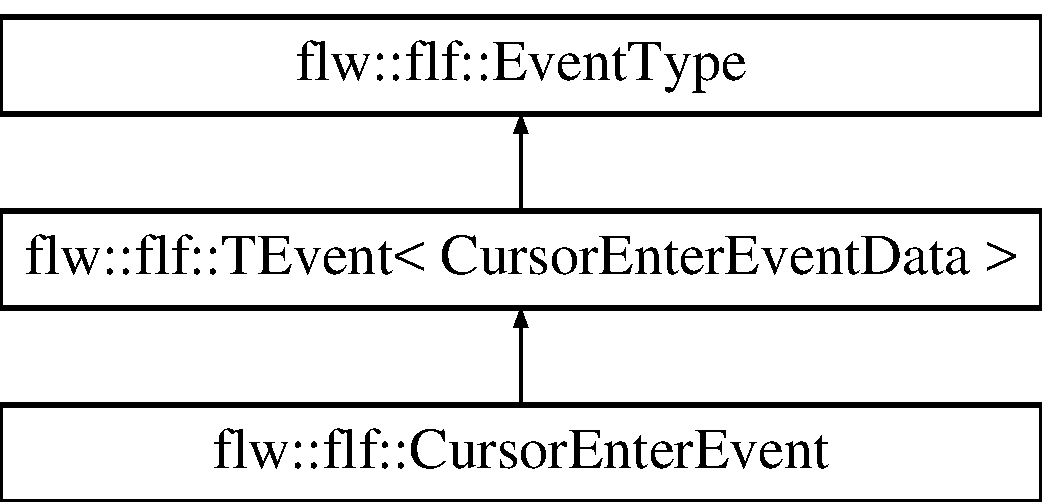
\includegraphics[height=3.000000cm]{classflw_1_1flf_1_1CursorEnterEvent}
\end{center}
\end{figure}
\subsection*{Public Member Functions}
\begin{DoxyCompactItemize}
\item 
{\bfseries Cursor\+Enter\+Event} (\hyperlink{structflw_1_1flf_1_1CursorEnterEventData}{Cursor\+Enter\+Event\+Data} \&data)\hypertarget{classflw_1_1flf_1_1CursorEnterEvent_a6c712068a4f6182771d55de3c3de2e3d}{}\label{classflw_1_1flf_1_1CursorEnterEvent_a6c712068a4f6182771d55de3c3de2e3d}

\end{DoxyCompactItemize}
\subsection*{Additional Inherited Members}


\subsection{Detailed Description}
Event introduced when cursor enters the window. 

The documentation for this struct was generated from the following file\+:\begin{DoxyCompactItemize}
\item 
/home/filip/\+Projects/fillwave/inc/fillwave/actions/events/Cursor\+Enter\+T\+Event.\+h\end{DoxyCompactItemize}

\hypertarget{structflw_1_1flf_1_1CursorEnterEventData}{}\section{flw\+:\+:flf\+:\+:Cursor\+Enter\+Event\+Data Struct Reference}
\label{structflw_1_1flf_1_1CursorEnterEventData}\index{flw\+::flf\+::\+Cursor\+Enter\+Event\+Data@{flw\+::flf\+::\+Cursor\+Enter\+Event\+Data}}
\subsection*{Public Attributes}
\begin{DoxyCompactItemize}
\item 
\mbox{\Hypertarget{structflw_1_1flf_1_1CursorEnterEventData_a30ebfc482500e3cfaa542a67b1e644cc}\label{structflw_1_1flf_1_1CursorEnterEventData_a30ebfc482500e3cfaa542a67b1e644cc}} 
int {\bfseries direction}
\end{DoxyCompactItemize}


The documentation for this struct was generated from the following file\+:\begin{DoxyCompactItemize}
\item 
/home/filip/projects/fillwave/inc/fillwave/actions/Event.\+h\end{DoxyCompactItemize}

\hypertarget{classflw_1_1flf_1_1CursorPositionEvent}{}\section{flw\+:\+:flf\+:\+:Cursor\+Position\+Event Struct Reference}
\label{classflw_1_1flf_1_1CursorPositionEvent}\index{flw\+::flf\+::\+Cursor\+Position\+Event@{flw\+::flf\+::\+Cursor\+Position\+Event}}


Event introduced when cursor position was changed.  




{\ttfamily \#include $<$Cursor\+Position\+T\+Event.\+h$>$}

Inheritance diagram for flw\+:\+:flf\+:\+:Cursor\+Position\+Event\+:\begin{figure}[H]
\begin{center}
\leavevmode
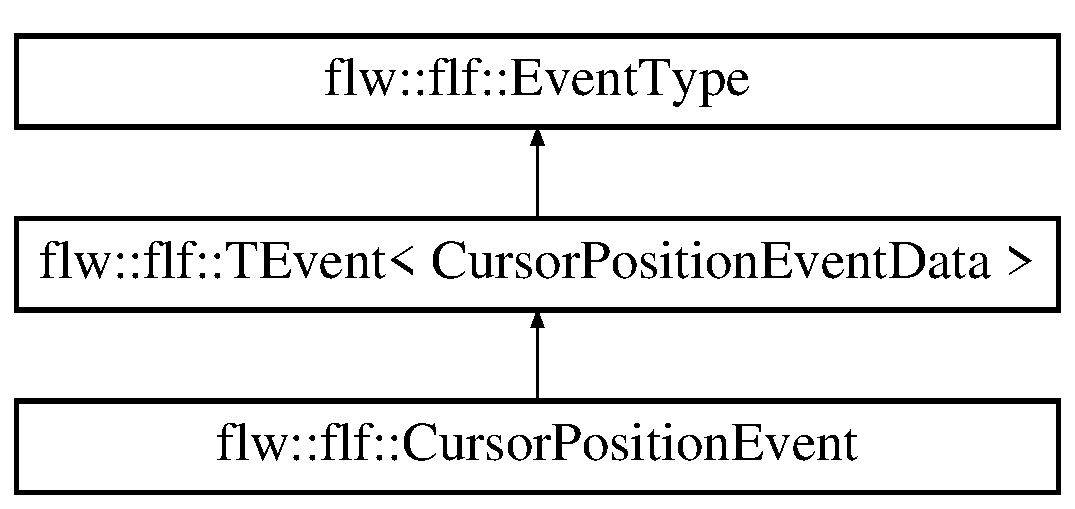
\includegraphics[height=3.000000cm]{classflw_1_1flf_1_1CursorPositionEvent}
\end{center}
\end{figure}
\subsection*{Public Member Functions}
\begin{DoxyCompactItemize}
\item 
{\bfseries Cursor\+Position\+Event} (\hyperlink{structflw_1_1flf_1_1CursorPositionEventData}{Cursor\+Position\+Event\+Data} \&data)\hypertarget{classflw_1_1flf_1_1CursorPositionEvent_aa5a515d0f5f5ee64060c398c46d80f49}{}\label{classflw_1_1flf_1_1CursorPositionEvent_aa5a515d0f5f5ee64060c398c46d80f49}

\end{DoxyCompactItemize}
\subsection*{Additional Inherited Members}


\subsection{Detailed Description}
Event introduced when cursor position was changed. 

The documentation for this struct was generated from the following file\+:\begin{DoxyCompactItemize}
\item 
/home/filip/\+Projects/fillwave/inc/fillwave/actions/events/Cursor\+Position\+T\+Event.\+h\end{DoxyCompactItemize}

\hypertarget{structflw_1_1flf_1_1CursorPositionEventData}{}\section{flw\+:\+:flf\+:\+:Cursor\+Position\+Event\+Data Struct Reference}
\label{structflw_1_1flf_1_1CursorPositionEventData}\index{flw\+::flf\+::\+Cursor\+Position\+Event\+Data@{flw\+::flf\+::\+Cursor\+Position\+Event\+Data}}
\subsection*{Public Attributes}
\begin{DoxyCompactItemize}
\item 
\mbox{\Hypertarget{structflw_1_1flf_1_1CursorPositionEventData_a81d94727e5940bfab91223fa48332df0}\label{structflw_1_1flf_1_1CursorPositionEventData_a81d94727e5940bfab91223fa48332df0}} 
double {\bfseries x\+Position}
\item 
\mbox{\Hypertarget{structflw_1_1flf_1_1CursorPositionEventData_ad0a614b6aea762878ba9328fb56739e5}\label{structflw_1_1flf_1_1CursorPositionEventData_ad0a614b6aea762878ba9328fb56739e5}} 
double {\bfseries y\+Position}
\end{DoxyCompactItemize}


The documentation for this struct was generated from the following file\+:\begin{DoxyCompactItemize}
\item 
/home/filip/projects/fillwave/inc/fillwave/actions/Event.\+h\end{DoxyCompactItemize}

\hypertarget{classflw_1_1flf_1_1Debugger}{}\section{flw\+:\+:flf\+:\+:Debugger Class Reference}
\label{classflw_1_1flf_1_1Debugger}\index{flw\+::flf\+::\+Debugger@{flw\+::flf\+::\+Debugger}}


Fillwave debugger.  




{\ttfamily \#include $<$Debugger.\+h$>$}

Inheritance diagram for flw\+:\+:flf\+:\+:Debugger\+:\begin{figure}[H]
\begin{center}
\leavevmode
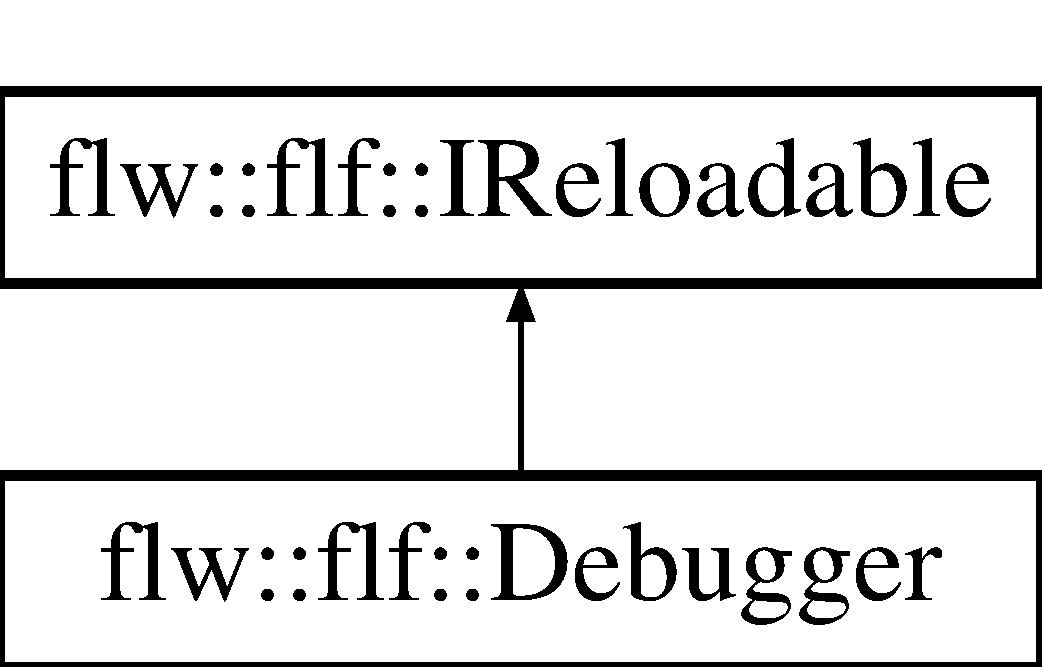
\includegraphics[height=2.000000cm]{classflw_1_1flf_1_1Debugger}
\end{center}
\end{figure}
\subsection*{Public Member Functions}
\begin{DoxyCompactItemize}
\item 
{\bfseries Debugger} (\hyperlink{classflw_1_1Engine}{Engine} $\ast$engine, G\+Lsizei how\+Many\+Debug\+Windows=6)\hypertarget{classflw_1_1flf_1_1Debugger_a4570381482b8e0ae6ec20dcda8b86e56}{}\label{classflw_1_1flf_1_1Debugger_a4570381482b8e0ae6ec20dcda8b86e56}

\item 
void {\bfseries set\+State} (e\+Debugger\+State state)\hypertarget{classflw_1_1flf_1_1Debugger_a2fa89641efc4c14babf974fa5405e88d}{}\label{classflw_1_1flf_1_1Debugger_a2fa89641efc4c14babf974fa5405e88d}

\item 
e\+Debugger\+State {\bfseries get\+State} ()\hypertarget{classflw_1_1flf_1_1Debugger_ae6cf63674c47fb1f08b16b903f9a4c6f}{}\label{classflw_1_1flf_1_1Debugger_ae6cf63674c47fb1f08b16b903f9a4c6f}

\item 
void {\bfseries prepare\+Debug\+Window} (G\+Lint id=0)\hypertarget{classflw_1_1flf_1_1Debugger_a17da1935b9481ac8411d7d213f4aedd1}{}\label{classflw_1_1flf_1_1Debugger_a17da1935b9481ac8411d7d213f4aedd1}

\item 
void {\bfseries render\+From\+Camera} (\hyperlink{classflw_1_1flf_1_1ICamera}{I\+Camera} \&c, G\+Lint id=0)\hypertarget{classflw_1_1flf_1_1Debugger_a2e77e7dabf1de62f9bc77d2a7639482d}{}\label{classflw_1_1flf_1_1Debugger_a2e77e7dabf1de62f9bc77d2a7639482d}

\item 
void {\bfseries render\+Depth\+Perspective} (G\+Lint id=0)\hypertarget{classflw_1_1flf_1_1Debugger_acce2fb29767c433cf66bd1471165230d}{}\label{classflw_1_1flf_1_1Debugger_acce2fb29767c433cf66bd1471165230d}

\item 
void {\bfseries render\+Depth\+Orthographic} (G\+Lint id=0)\hypertarget{classflw_1_1flf_1_1Debugger_ace0a7b5a5a567bb9b10f0c4ed571b62e}{}\label{classflw_1_1flf_1_1Debugger_ace0a7b5a5a567bb9b10f0c4ed571b62e}

\item 
void {\bfseries render\+Picking\+Map} ()\hypertarget{classflw_1_1flf_1_1Debugger_a9e591ee479c22a4fcfaf51a85db03975}{}\label{classflw_1_1flf_1_1Debugger_a9e591ee479c22a4fcfaf51a85db03975}

\item 
void {\bfseries render\+Geometry\+Buffer} (G\+Luint width, G\+Luint height, G\+Luint attachments, \hyperlink{classflw_1_1flc_1_1FramebufferGeometry}{flc\+::\+Framebuffer\+Geometry} $\ast$buffer)\hypertarget{classflw_1_1flf_1_1Debugger_a874b8a109365ef5252835ee536b0bf1f}{}\label{classflw_1_1flf_1_1Debugger_a874b8a109365ef5252835ee536b0bf1f}

\end{DoxyCompactItemize}
\subsection*{Additional Inherited Members}


\subsection{Detailed Description}
Fillwave debugger. 


\begin{DoxyItemize}
\item Debugging depth maps
\item drawing scene from certain views
\item creating multi-\/windowed view 
\end{DoxyItemize}

The documentation for this class was generated from the following file\+:\begin{DoxyCompactItemize}
\item 
/home/filip/\+Projects/fillwave/inc/fillwave/Debugger.\+h\end{DoxyCompactItemize}

\hypertarget{classflw_1_1flf_1_1EmiterPointCPU}{}\section{flw\+:\+:flf\+:\+:Emiter\+Point\+C\+PU Class Reference}
\label{classflw_1_1flf_1_1EmiterPointCPU}\index{flw\+::flf\+::\+Emiter\+Point\+C\+PU@{flw\+::flf\+::\+Emiter\+Point\+C\+PU}}


Polynomial particle Emiter. Can generate a particles with velocity, direction, and acceleration defined by the user.  




{\ttfamily \#include $<$Emiter\+Point\+C\+P\+U.\+h$>$}

Inheritance diagram for flw\+:\+:flf\+:\+:Emiter\+Point\+C\+PU\+:\begin{figure}[H]
\begin{center}
\leavevmode
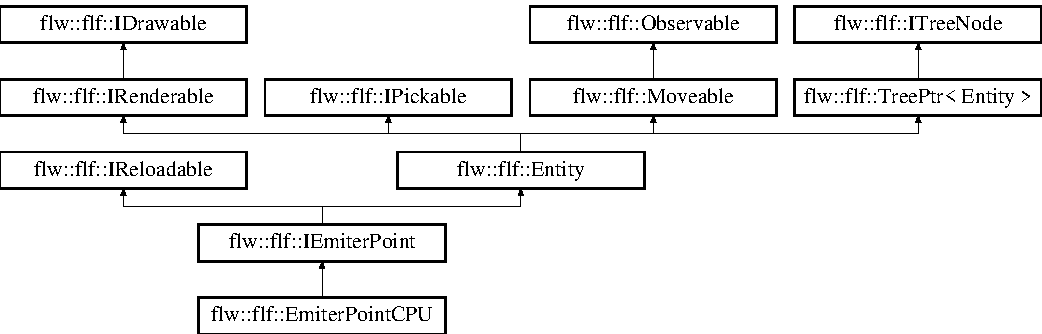
\includegraphics[height=4.487180cm]{classflw_1_1flf_1_1EmiterPointCPU}
\end{center}
\end{figure}
\subsection*{Public Member Functions}
\begin{DoxyCompactItemize}
\item 
\mbox{\Hypertarget{classflw_1_1flf_1_1EmiterPointCPU_a85fabd562bea67577072b4490ee07579}\label{classflw_1_1flf_1_1EmiterPointCPU_a85fabd562bea67577072b4490ee07579}} 
{\bfseries Emiter\+Point\+C\+PU} (\hyperlink{classflw_1_1Engine}{Engine} $\ast$engine, G\+Lfloat emiting\+Source\+Rate, G\+Luint how\+Many, glm\+::vec4 color, glm\+::vec3 acceleration=glm\+::vec3(0.\+0), glm\+::vec3 start\+Velocity=glm\+::vec3(0.\+0), glm\+::vec3 robustness\+Velocity=glm\+::vec3(0.\+0), glm\+::vec3 start\+Position=glm\+::vec3(0.\+0), glm\+::vec3 robustness\+Position=glm\+::vec3(0.\+0), G\+Lfloat start\+Size=1.\+0, G\+Lfloat lifetime=6.\+0, \hyperlink{classflw_1_1flc_1_1Texture}{flc\+::\+Texture} $\ast$texture=nullptr, G\+Lenum blending\+Source=G\+L\+\_\+\+S\+R\+C\+\_\+\+A\+L\+P\+HA, G\+Lenum blending\+Destination=G\+L\+\_\+\+O\+N\+E\+\_\+\+M\+I\+N\+U\+S\+\_\+\+S\+R\+C\+\_\+\+A\+L\+P\+HA, G\+Lboolean depth\+Testing=G\+L\+\_\+\+T\+R\+UE, G\+Lfloat alpha\+Cut\+Off\+Level=0.\+0f)
\item 
\mbox{\Hypertarget{classflw_1_1flf_1_1EmiterPointCPU_a39dc08138d5366e98360db1e40e5f3df}\label{classflw_1_1flf_1_1EmiterPointCPU_a39dc08138d5366e98360db1e40e5f3df}} 
void {\bfseries update} (G\+Lfloat time\+Elapsed\+Sec) override
\item 
\mbox{\Hypertarget{classflw_1_1flf_1_1EmiterPointCPU_ad17e8a7d32a32e795be9d071acca15f6}\label{classflw_1_1flf_1_1EmiterPointCPU_ad17e8a7d32a32e795be9d071acca15f6}} 
void {\bfseries draw} (\hyperlink{classflw_1_1flf_1_1ICamera}{I\+Camera} \&camera) override
\item 
\mbox{\Hypertarget{classflw_1_1flf_1_1EmiterPointCPU_ac910a2c531211f991146a7ee566b3c6e}\label{classflw_1_1flf_1_1EmiterPointCPU_ac910a2c531211f991146a7ee566b3c6e}} 
void {\bfseries draw\+P\+B\+RP} (\hyperlink{classflw_1_1flf_1_1ICamera}{I\+Camera} \&camera) override
\item 
\mbox{\Hypertarget{classflw_1_1flf_1_1EmiterPointCPU_a52c18a5d5a4d36cfb2b07f6f1355be80}\label{classflw_1_1flf_1_1EmiterPointCPU_a52c18a5d5a4d36cfb2b07f6f1355be80}} 
bool {\bfseries get\+Render\+Item} (\hyperlink{structflw_1_1flf_1_1RenderItem}{Render\+Item} \&item) override
\end{DoxyCompactItemize}
\subsection*{Additional Inherited Members}


\subsection{Detailed Description}
Polynomial particle Emiter. Can generate a particles with velocity, direction, and acceleration defined by the user. 

The documentation for this class was generated from the following file\+:\begin{DoxyCompactItemize}
\item 
/home/filip/projects/fillwave/inc/fillwave/models/Emiter\+Point\+C\+P\+U.\+h\end{DoxyCompactItemize}

\hypertarget{classflw_1_1flf_1_1EmiterPointGPU}{}\section{flw\+:\+:flf\+:\+:Emiter\+Point\+G\+PU Class Reference}
\label{classflw_1_1flf_1_1EmiterPointGPU}\index{flw\+::flf\+::\+Emiter\+Point\+G\+PU@{flw\+::flf\+::\+Emiter\+Point\+G\+PU}}


Polynomial particle Emiter entirely computed on G\+PU. Can generate a particles with velocity, direction, and acceleration defined by the user.  




{\ttfamily \#include $<$Emiter\+Point\+G\+P\+U.\+h$>$}

Inheritance diagram for flw\+:\+:flf\+:\+:Emiter\+Point\+G\+PU\+:\begin{figure}[H]
\begin{center}
\leavevmode
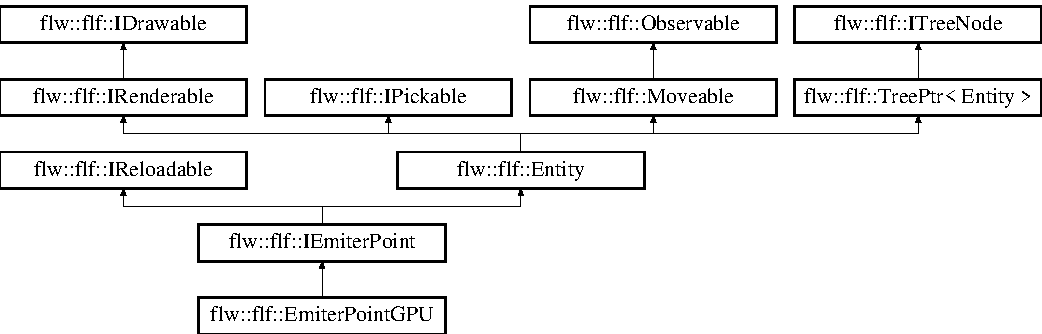
\includegraphics[height=4.487180cm]{classflw_1_1flf_1_1EmiterPointGPU}
\end{center}
\end{figure}
\subsection*{Public Member Functions}
\begin{DoxyCompactItemize}
\item 
{\bfseries Emiter\+Point\+G\+PU} (\hyperlink{classflw_1_1Engine}{Engine} $\ast$engine, G\+Lfloat emiting\+Source\+Rate, G\+Luint how\+Many, glm\+::vec4 color, glm\+::vec3 acceleration, glm\+::vec3 start\+Velocity, glm\+::vec3 robustness\+Velocity, glm\+::vec3 start\+Position, glm\+::vec3 robustness\+Position, G\+Lfloat start\+Size, G\+Lfloat lifetime, \hyperlink{classflw_1_1flc_1_1Texture}{flc\+::\+Texture} $\ast$texture, G\+Lenum blending\+Source, G\+Lenum blending\+Destination, G\+Lboolean depth\+Testing, G\+Lfloat alpha\+Cut\+Off\+Level=0.\+0f)\hypertarget{classflw_1_1flf_1_1EmiterPointGPU_a63b5c560ccc89f38bd0c974372eda1cf}{}\label{classflw_1_1flf_1_1EmiterPointGPU_a63b5c560ccc89f38bd0c974372eda1cf}

\item 
void {\bfseries update} (G\+Lfloat time\+Elapsed\+Sec) override\hypertarget{classflw_1_1flf_1_1EmiterPointGPU_a6c816e0fb1b4626c814012dcf3d81d10}{}\label{classflw_1_1flf_1_1EmiterPointGPU_a6c816e0fb1b4626c814012dcf3d81d10}

\item 
void {\bfseries draw} (\hyperlink{classflw_1_1flf_1_1ICamera}{I\+Camera} \&camera) override\hypertarget{classflw_1_1flf_1_1EmiterPointGPU_ae6a1e9b822d2d121f5c9403a3a032d2a}{}\label{classflw_1_1flf_1_1EmiterPointGPU_ae6a1e9b822d2d121f5c9403a3a032d2a}

\item 
void {\bfseries draw\+P\+B\+RP} (\hyperlink{classflw_1_1flf_1_1ICamera}{I\+Camera} \&camera) override\hypertarget{classflw_1_1flf_1_1EmiterPointGPU_a7233c34c58d55abd33c7cbfcbffe272b}{}\label{classflw_1_1flf_1_1EmiterPointGPU_a7233c34c58d55abd33c7cbfcbffe272b}

\item 
bool {\bfseries get\+Render\+Item} (\hyperlink{structflw_1_1flf_1_1RenderItem}{Render\+Item} \&item) override\hypertarget{classflw_1_1flf_1_1EmiterPointGPU_a1a3f0a9adb28d5051b767d4c18b6c51f}{}\label{classflw_1_1flf_1_1EmiterPointGPU_a1a3f0a9adb28d5051b767d4c18b6c51f}

\end{DoxyCompactItemize}
\subsection*{Additional Inherited Members}


\subsection{Detailed Description}
Polynomial particle Emiter entirely computed on G\+PU. Can generate a particles with velocity, direction, and acceleration defined by the user. 

The documentation for this class was generated from the following file\+:\begin{DoxyCompactItemize}
\item 
/home/filip/\+Projects/fillwave/inc/fillwave/models/Emiter\+Point\+G\+P\+U.\+h\end{DoxyCompactItemize}

\hypertarget{classflw_1_1flf_1_1EmiterPointStep}{}\section{flw\+:\+:flf\+:\+:Emiter\+Point\+Step Class Reference}
\label{classflw_1_1flf_1_1EmiterPointStep}\index{flw\+::flf\+::\+Emiter\+Point\+Step@{flw\+::flf\+::\+Emiter\+Point\+Step}}


Not used.  




{\ttfamily \#include $<$Emiter\+Point\+Step.\+h$>$}

Inheritance diagram for flw\+:\+:flf\+:\+:Emiter\+Point\+Step\+:\begin{figure}[H]
\begin{center}
\leavevmode
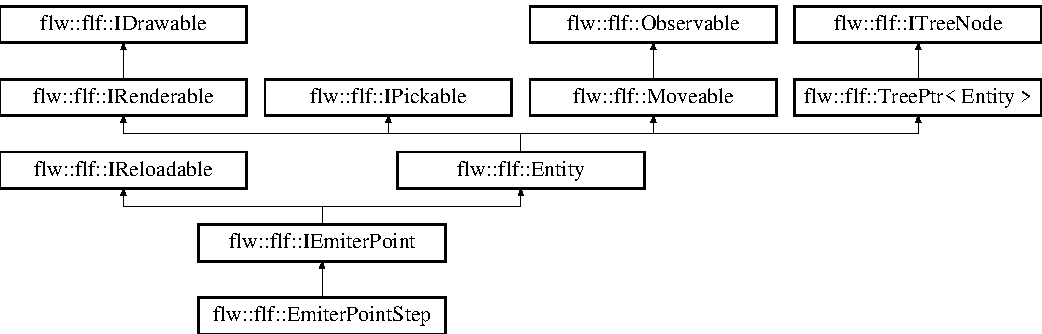
\includegraphics[height=4.487180cm]{classflw_1_1flf_1_1EmiterPointStep}
\end{center}
\end{figure}
\subsection*{Public Member Functions}
\begin{DoxyCompactItemize}
\item 
{\bfseries Emiter\+Point\+Step} (\hyperlink{classflw_1_1Engine}{Engine} $\ast$engine, G\+Lint how\+Many, G\+Lenum blending\+Source, G\+Lenum blending\+Destination, \hyperlink{classflw_1_1flc_1_1Texture}{flc\+::\+Texture} $\ast$texture)\hypertarget{classflw_1_1flf_1_1EmiterPointStep_afb53156f26a793f33e0d86646b87c4cc}{}\label{classflw_1_1flf_1_1EmiterPointStep_afb53156f26a793f33e0d86646b87c4cc}

\end{DoxyCompactItemize}
\subsection*{Additional Inherited Members}


\subsection{Detailed Description}
Not used. 

The documentation for this class was generated from the following file\+:\begin{DoxyCompactItemize}
\item 
/home/filip/\+Projects/fillwave/inc/fillwave/models/Emiter\+Point\+Step.\+h\end{DoxyCompactItemize}

\hypertarget{classflw_1_1Engine}{}\section{flw\+:\+:Engine Class Reference}
\label{classflw_1_1Engine}\index{flw\+::\+Engine@{flw\+::\+Engine}}


Fillwave engine.  




{\ttfamily \#include $<$Fillwave.\+h$>$}

\subsection*{Classes}
\begin{DoxyCompactItemize}
\item 
struct \hyperlink{structflw_1_1Engine_1_1EngineImpl}{Engine\+Impl}
\begin{DoxyCompactList}\small\item\em Private implementation of Fillwave GE. \end{DoxyCompactList}\end{DoxyCompactItemize}
\subsection*{Public Member Functions}
\begin{DoxyCompactItemize}
\item 
{\bfseries Engine} (G\+Lint argc, G\+Lchar $\ast$const argv\mbox{[}$\,$\mbox{]})\hypertarget{classflw_1_1Engine_a8efacbf047d08cc6e04cf81af63bcc4f}{}\label{classflw_1_1Engine_a8efacbf047d08cc6e04cf81af63bcc4f}

\item 
void {\bfseries config\+Debugger} (e\+Debugger\+State state)\hypertarget{classflw_1_1Engine_a0e9fd50ccc0377a675a33b423844ba84}{}\label{classflw_1_1Engine_a0e9fd50ccc0377a675a33b423844ba84}

\item 
void {\bfseries config\+File\+Logging} (std\+::string file\+Name=\char`\"{}\char`\"{})\hypertarget{classflw_1_1Engine_ab7c9423b53e553e0cf8932c7a8e6a3c1}{}\label{classflw_1_1Engine_ab7c9423b53e553e0cf8932c7a8e6a3c1}

\item 
void {\bfseries config\+F\+P\+S\+Counter} (std\+::string font\+Name=\char`\"{}\char`\"{}, glm\+::vec2 position=glm\+::vec2(-\/0.\+95, 0.\+95), G\+Lfloat size=100.\+0)\hypertarget{classflw_1_1Engine_ac155824c8e1f16457f8788836eb9d0d3}{}\label{classflw_1_1Engine_ac155824c8e1f16457f8788836eb9d0d3}

\item 
void {\bfseries config\+Background\+Color} (glm\+::vec3 color)\hypertarget{classflw_1_1Engine_a095771e29420c83636acb355701e0751}{}\label{classflw_1_1Engine_a095771e29420c83636acb355701e0751}

\item 
void {\bfseries config\+Time} (G\+Lfloat time\+Factor)\hypertarget{classflw_1_1Engine_ac35ea4a508bc9bda596b84d9dc6a0ca3}{}\label{classflw_1_1Engine_ac35ea4a508bc9bda596b84d9dc6a0ca3}

\item 
void {\bfseries draw} (G\+Lfloat time)\hypertarget{classflw_1_1Engine_a65d5d45571a4a9831da5954b2848e7eb}{}\label{classflw_1_1Engine_a65d5d45571a4a9831da5954b2848e7eb}

\item 
void {\bfseries draw\+Lines} (G\+Lfloat time)\hypertarget{classflw_1_1Engine_ad9bbbabe65c1c59a3b9ace8900ade8f3}{}\label{classflw_1_1Engine_ad9bbbabe65c1c59a3b9ace8900ade8f3}

\item 
void {\bfseries draw\+Points} (G\+Lfloat time)\hypertarget{classflw_1_1Engine_af5d70bafff4bb7a38a59805f6e1f3c18}{}\label{classflw_1_1Engine_af5d70bafff4bb7a38a59805f6e1f3c18}

\item 
void {\bfseries draw\+Texture} (\hyperlink{classflw_1_1flc_1_1Texture}{flc\+::\+Texture} $\ast$t, \hyperlink{classflw_1_1flc_1_1Program}{flc\+::\+Program} $\ast$p)\hypertarget{classflw_1_1Engine_a0f9be72217d6d7b75e3733ca5d84b017}{}\label{classflw_1_1Engine_a0f9be72217d6d7b75e3733ca5d84b017}

\item 
void {\bfseries draw\+Texture} (\hyperlink{classflw_1_1flc_1_1Texture}{flc\+::\+Texture} $\ast$t)\hypertarget{classflw_1_1Engine_a4d587f6fb90fc7a768de763dce482f09}{}\label{classflw_1_1Engine_a4d587f6fb90fc7a768de763dce482f09}

\item 
void {\bfseries detach} (p\+Text text)\hypertarget{classflw_1_1Engine_a5332338c3dbbeddd07a17a2e54ec4c56}{}\label{classflw_1_1Engine_a5332338c3dbbeddd07a17a2e54ec4c56}

\item 
void {\bfseries detach} (\hyperlink{classflw_1_1flf_1_1LightSpot}{flf\+::\+Light\+Spot} $\ast$light)\hypertarget{classflw_1_1Engine_ae9875ee870b6a6ced53f326b6f5d5624}{}\label{classflw_1_1Engine_ae9875ee870b6a6ced53f326b6f5d5624}

\item 
void {\bfseries detach} (\hyperlink{classflw_1_1flf_1_1LightDirectional}{flf\+::\+Light\+Directional} $\ast$light)\hypertarget{classflw_1_1Engine_ad60883038374172d30c55545df440da2}{}\label{classflw_1_1Engine_ad60883038374172d30c55545df440da2}

\item 
void {\bfseries detach} (\hyperlink{classflw_1_1flf_1_1LightPoint}{flf\+::\+Light\+Point} $\ast$light)\hypertarget{classflw_1_1Engine_ad315c597cc2919ec2b1c0528b3d4b8d9}{}\label{classflw_1_1Engine_ad315c597cc2919ec2b1c0528b3d4b8d9}

\item 
void {\bfseries detach\+Lights} ()\hypertarget{classflw_1_1Engine_a22021b98e5911ba083cd85d09b9e2edb}{}\label{classflw_1_1Engine_a22021b98e5911ba083cd85d09b9e2edb}

\item 
void {\bfseries detach} (\hyperlink{classflw_1_1flf_1_1Entity}{flf\+::\+Entity} $\ast$)\hypertarget{classflw_1_1Engine_a28a44080d29beb1bb029661878f29287}{}\label{classflw_1_1Engine_a28a44080d29beb1bb029661878f29287}

\item 
pu\+Physics\+Mesh\+Buffer {\bfseries get\+Physical\+Mesh\+Buffer} (const std\+::string \&shape\+Path)\hypertarget{classflw_1_1Engine_aa0886491c6b278c99c51e389415aa46f}{}\label{classflw_1_1Engine_aa0886491c6b278c99c51e389415aa46f}

\item 
void {\bfseries set\+Current\+Scene} (pu\+Scene \&\&scene)\hypertarget{classflw_1_1Engine_a15a611c51dec7cca5d9f53aa433c64ea}{}\label{classflw_1_1Engine_a15a611c51dec7cca5d9f53aa433c64ea}

\item 
\hyperlink{classflw_1_1TGetter}{T\+Getter}$<$ \hyperlink{classflw_1_1flf_1_1Scene}{flf\+::\+Scene} $>$ {\bfseries get\+Current\+Scene} () const \hypertarget{classflw_1_1Engine_a15f25cc34d9d952d8538389867e7de38}{}\label{classflw_1_1Engine_a15f25cc34d9d952d8538389867e7de38}

\item 
G\+Luint {\bfseries get\+Frames\+Passed} ()\hypertarget{classflw_1_1Engine_ad359cfb8982e2dd698a05b1c73eb534a}{}\label{classflw_1_1Engine_ad359cfb8982e2dd698a05b1c73eb534a}

\item 
G\+Lfloat {\bfseries get\+Startup\+Animation\+Time} () const \hypertarget{classflw_1_1Engine_af9df12dca5e42043fea9ae3f81d3b1cc}{}\label{classflw_1_1Engine_af9df12dca5e42043fea9ae3f81d3b1cc}

\item 
{\footnotesize template$<$G\+Luint T$>$ }\\\hyperlink{classflw_1_1flc_1_1Shader}{flc\+::\+Shader} $\ast$ \hyperlink{classflw_1_1Engine_a36555136687e9128629e0b2d9a0992d1}{store\+Shader} (const std\+::string \&shader\+Path)
\item 
{\footnotesize template$<$G\+Luint T$>$ }\\\hyperlink{classflw_1_1flc_1_1Shader}{flc\+::\+Shader} $\ast$ {\bfseries store\+Shader} (const std\+::string \&shader\+Path, const std\+::string \&shader\+Source)\hypertarget{classflw_1_1Engine_a752be0593e2f81094e3af50f0f36079f}{}\label{classflw_1_1Engine_a752be0593e2f81094e3af50f0f36079f}

\item 
\hyperlink{classflw_1_1flc_1_1Program}{flc\+::\+Program} $\ast$ {\bfseries store\+Program} (const std\+::string \&name, const std\+::vector$<$ \hyperlink{classflw_1_1flc_1_1Shader}{flc\+::\+Shader} $\ast$ $>$ \&shaders, bool is\+Skip\+Linking=false)\hypertarget{classflw_1_1Engine_a6ffbeb11f3c66a0412e807a4268b6b8e}{}\label{classflw_1_1Engine_a6ffbeb11f3c66a0412e807a4268b6b8e}

\item 
\hyperlink{classflw_1_1flc_1_1Texture2D}{flc\+::\+Texture2D} $\ast$ {\bfseries store\+Texture} (const std\+::string \&path, flf\+::e\+Compression com=flf\+::e\+Compression\+::e\+None)\hypertarget{classflw_1_1Engine_a9fb7df4341b1fd4555bc079738a031c6}{}\label{classflw_1_1Engine_a9fb7df4341b1fd4555bc079738a031c6}

\item 
\hyperlink{classflw_1_1flc_1_1Texture2DRenderable}{flc\+::\+Texture2\+D\+Renderable} $\ast$ {\bfseries store\+Texture\+Renderable} ()\hypertarget{classflw_1_1Engine_aa99a2c0cd6a324729645ff39a6a3fbc2}{}\label{classflw_1_1Engine_aa99a2c0cd6a324729645ff39a6a3fbc2}

\item 
\hyperlink{classflw_1_1flc_1_1Texture2DRenderableDynamic}{flc\+::\+Texture2\+D\+Renderable\+Dynamic} $\ast$ {\bfseries store\+Texture\+Dynamic} (const std\+::string \&fragment\+Shader\+Path)\hypertarget{classflw_1_1Engine_a972d208b867f3e8dc2e22ea785049c70}{}\label{classflw_1_1Engine_a972d208b867f3e8dc2e22ea785049c70}

\item 
\hyperlink{classflw_1_1flc_1_1Texture3D}{flc\+::\+Texture3D} $\ast$ {\bfseries store\+Texture3D} (const std\+::string \&posX, const std\+::string \&negX, const std\+::string \&posY, const std\+::string \&negY, const std\+::string \&posZ, const std\+::string \&negZ)\hypertarget{classflw_1_1Engine_a92182f6d9157ff16568f224b431138cc}{}\label{classflw_1_1Engine_a92182f6d9157ff16568f224b431138cc}

\item 
\hyperlink{classflw_1_1flf_1_1LightSpot}{flf\+::\+Light\+Spot} $\ast$ {\bfseries store\+Light\+Spot} (glm\+::vec3 pos, glm\+::quat rot, glm\+::vec4 col, \hyperlink{classflw_1_1flf_1_1Moveable}{flf\+::\+Moveable} $\ast$followed=nullptr)\hypertarget{classflw_1_1Engine_a0aeefd08b5cfc40ed9a5a82a91693cc6}{}\label{classflw_1_1Engine_a0aeefd08b5cfc40ed9a5a82a91693cc6}

\item 
\hyperlink{classflw_1_1flf_1_1LightPoint}{flf\+::\+Light\+Point} $\ast$ {\bfseries store\+Light\+Point} (glm\+::vec3 position, glm\+::vec4 color, \hyperlink{classflw_1_1flf_1_1Moveable}{flf\+::\+Moveable} $\ast$followed=nullptr)\hypertarget{classflw_1_1Engine_abd668a07a20b7241aaca67f49d0cf9f1}{}\label{classflw_1_1Engine_abd668a07a20b7241aaca67f49d0cf9f1}

\item 
\hyperlink{classflw_1_1flf_1_1LightDirectional}{flf\+::\+Light\+Directional} $\ast$ {\bfseries store\+Light\+Directional} (glm\+::vec3 position, glm\+::quat rotation, glm\+::vec4 color, \hyperlink{classflw_1_1flf_1_1Moveable}{flf\+::\+Moveable} $\ast$followed=nullptr)\hypertarget{classflw_1_1Engine_a017f4a374d3acaac4120afeb2594ec4d}{}\label{classflw_1_1Engine_a017f4a374d3acaac4120afeb2594ec4d}

\item 
p\+Text {\bfseries store\+Text} (const std\+::string \&content, const std\+::string \&font\+Name, glm\+::vec2 position, G\+Lfloat scale=1.\+0f, glm\+::vec4 color=glm\+::vec4(1.\+0f, 1.\+0f, 1.\+0f, 1.\+0f), e\+Text\+Effect effect=e\+Text\+Effect\+::e\+None)\hypertarget{classflw_1_1Engine_a9dda9b1fc63f416e05404389f7a3bb5f}{}\label{classflw_1_1Engine_a9dda9b1fc63f416e05404389f7a3bb5f}

\item 
\hyperlink{classflw_1_1flc_1_1Sampler}{flc\+::\+Sampler} $\ast$ {\bfseries store\+SO} (G\+Lint texture\+Unit)\hypertarget{classflw_1_1Engine_a8ca2976f879365fdeaab18646da9c327}{}\label{classflw_1_1Engine_a8ca2976f879365fdeaab18646da9c327}

\item 
\hyperlink{classflw_1_1flc_1_1VertexArray}{flc\+::\+Vertex\+Array} $\ast$ {\bfseries store\+V\+AO} (\hyperlink{classflw_1_1flf_1_1IReloadable}{flf\+::\+I\+Reloadable} $\ast$user, \hyperlink{classflw_1_1flc_1_1VertexArray}{flc\+::\+Vertex\+Array} $\ast$vao=nullptr)\hypertarget{classflw_1_1Engine_ae6de8a2803a2802739377dacadde496a}{}\label{classflw_1_1Engine_ae6de8a2803a2802739377dacadde496a}

\item 
{\footnotesize template$<$class T , typename... S$>$ }\\T $\ast$ {\bfseries store\+Buffer} (\hyperlink{classflw_1_1flc_1_1VertexArray}{flc\+::\+Vertex\+Array} $\ast$vao, S...\+p)\hypertarget{classflw_1_1Engine_a9dbbd4dd393fc420a68007781d3f7508}{}\label{classflw_1_1Engine_a9dbbd4dd393fc420a68007781d3f7508}

\item 
{\footnotesize template$<$class T , typename... S$>$ }\\T $\ast$ {\bfseries store\+Buffers} (\hyperlink{classflw_1_1flc_1_1VertexArray}{flc\+::\+Vertex\+Array} $\ast$vao, size\+\_\+t idx, S...\+p)\hypertarget{classflw_1_1Engine_ae9b593271f7b78401e12f325c780de33}{}\label{classflw_1_1Engine_ae9b593271f7b78401e12f325c780de33}

\item 
void {\bfseries remove\+Buffer} (\hyperlink{classflw_1_1flc_1_1VertexArray}{flc\+::\+Vertex\+Array} $\ast$vao)\hypertarget{classflw_1_1Engine_a8835f81ea40d7bf078381f5fd27dd004}{}\label{classflw_1_1Engine_a8835f81ea40d7bf078381f5fd27dd004}

\item 
void {\bfseries remove\+Buffer\+Index} (\hyperlink{classflw_1_1flc_1_1VertexArray}{flc\+::\+Vertex\+Array} $\ast$vao)\hypertarget{classflw_1_1Engine_aa388b763d05e260c6818f7ede1961101}{}\label{classflw_1_1Engine_aa388b763d05e260c6818f7ede1961101}

\item 
void {\bfseries remove\+Buffer\+Index\+Particles} (\hyperlink{classflw_1_1flc_1_1VertexArray}{flc\+::\+Vertex\+Array} $\ast$vao)\hypertarget{classflw_1_1Engine_a6da509ab60518e077e10005ad0e8c574}{}\label{classflw_1_1Engine_a6da509ab60518e077e10005ad0e8c574}

\item 
void {\bfseries remove\+Buffer\+Basic} (\hyperlink{classflw_1_1flc_1_1VertexArray}{flc\+::\+Vertex\+Array} $\ast$vao)\hypertarget{classflw_1_1Engine_a8875663742749eca089b8aebdf903325}{}\label{classflw_1_1Engine_a8875663742749eca089b8aebdf903325}

\item 
void {\bfseries remove\+Buffer\+Text} (\hyperlink{classflw_1_1flc_1_1VertexArray}{flc\+::\+Vertex\+Array} $\ast$vao)\hypertarget{classflw_1_1Engine_a1ebb7161680655b335bdc953a5e7c242}{}\label{classflw_1_1Engine_a1ebb7161680655b335bdc953a5e7c242}

\item 
void {\bfseries pick} (G\+Luint x, G\+Luint y)\hypertarget{classflw_1_1Engine_a61e393402f74243407e16c038cad6ada}{}\label{classflw_1_1Engine_a61e393402f74243407e16c038cad6ada}

\item 
glm\+::ivec2 {\bfseries get\+Screen\+Size} () const \hypertarget{classflw_1_1Engine_acb58494b14f77ffda697755c9d53bc2e}{}\label{classflw_1_1Engine_acb58494b14f77ffda697755c9d53bc2e}

\item 
G\+Lfloat {\bfseries get\+Screen\+Aspect\+Ratio} () const \hypertarget{classflw_1_1Engine_a25e764da8237f6da7d411952f8f306ab}{}\label{classflw_1_1Engine_a25e764da8237f6da7d411952f8f306ab}

\item 
void {\bfseries log} ()\hypertarget{classflw_1_1Engine_a7238e9e2e50dd6ab0d832cb9e9e412c8}{}\label{classflw_1_1Engine_a7238e9e2e50dd6ab0d832cb9e9e412c8}

\item 
void {\bfseries capture\+Framebuffer\+To\+File} (const std\+::string \&name)\hypertarget{classflw_1_1Engine_aa7c76ee55048778b1d30a0cf84967a36}{}\label{classflw_1_1Engine_aa7c76ee55048778b1d30a0cf84967a36}

\item 
void {\bfseries capture\+Framebuffer\+To\+Buffer} (G\+Lubyte $\ast$buf, G\+Lint $\ast$size\+In\+Bytes, G\+Luint format=G\+L\+\_\+\+R\+G\+BA, G\+Lint bytes\+Per\+Pixel=4)\hypertarget{classflw_1_1Engine_ab9c11c99353f93372987954a15c87862}{}\label{classflw_1_1Engine_ab9c11c99353f93372987954a15c87862}

\item 
void {\bfseries add\+Post\+Process} (const std\+::string \&fragment\+Shader\+Path, G\+Lfloat life\+Time=flf\+::\+F\+I\+L\+L\+W\+A\+V\+E\+\_\+\+E\+N\+D\+L\+E\+SS)\hypertarget{classflw_1_1Engine_aa8b374f4d6ab820ed055cde1e25bba5f}{}\label{classflw_1_1Engine_aa8b374f4d6ab820ed055cde1e25bba5f}

\item 
void {\bfseries drop\+Focus} (\hyperlink{classflw_1_1flf_1_1IFocusable}{flf\+::\+I\+Focusable} $\ast$focusable=nullptr)\hypertarget{classflw_1_1Engine_a5d612ba035d704f364ef80e217f4701f}{}\label{classflw_1_1Engine_a5d612ba035d704f364ef80e217f4701f}

\item 
void {\bfseries insert\+Input} (\hyperlink{classflw_1_1flf_1_1EventType}{flf\+::\+Event\+Type} \&event)\hypertarget{classflw_1_1Engine_a9450a7a12a0b0b0c8ced673c54272a78}{}\label{classflw_1_1Engine_a9450a7a12a0b0b0c8ced673c54272a78}

\item 
void {\bfseries insert\+Resize\+Screen} (G\+Luint width, G\+Luint height)\hypertarget{classflw_1_1Engine_a5c99dffdf37876df266a28ab3aa59b3b}{}\label{classflw_1_1Engine_a5c99dffdf37876df266a28ab3aa59b3b}

\item 
void {\bfseries attach\+Callback} (pu\+Callback \&\&callback, \hyperlink{classflw_1_1flf_1_1IFocusable}{flf\+::\+I\+Focusable} $\ast$focusable=nullptr)\hypertarget{classflw_1_1Engine_aa879716d8ee4c96122449a01696ca7c4}{}\label{classflw_1_1Engine_aa879716d8ee4c96122449a01696ca7c4}

\item 
void {\bfseries detach\+Callback} (\hyperlink{classflw_1_1flf_1_1Callback}{flf\+::\+Callback} $\ast$callback)\hypertarget{classflw_1_1Engine_ae4f759973523b435f2d8cd9aa95ecbff}{}\label{classflw_1_1Engine_ae4f759973523b435f2d8cd9aa95ecbff}

\item 
void {\bfseries detach\+Callbacks} (e\+Event\+Type event\+Type)\hypertarget{classflw_1_1Engine_a4163beecf0025671be70b19abe70be09}{}\label{classflw_1_1Engine_a4163beecf0025671be70b19abe70be09}

\item 
void {\bfseries detach\+Callbacks} ()\hypertarget{classflw_1_1Engine_aafe6fe8af3b28d7a368a067ff3367405}{}\label{classflw_1_1Engine_aafe6fe8af3b28d7a368a067ff3367405}

\item 
void {\bfseries reload} ()\hypertarget{classflw_1_1Engine_a370ce8e98ce6f22c828a9b089fa149eb}{}\label{classflw_1_1Engine_a370ce8e98ce6f22c828a9b089fa149eb}

\item 
\hyperlink{classflw_1_1flf_1_1LightSystem}{flf\+::\+Light\+System} \& {\bfseries get\+Light\+System} () const \hypertarget{classflw_1_1Engine_a6ba9afc7a2ca7b8a68d63146614ed3cd}{}\label{classflw_1_1Engine_a6ba9afc7a2ca7b8a68d63146614ed3cd}

\item 
\hyperlink{classflw_1_1flf_1_1TextureSystem}{flf\+::\+Texture\+System} \& {\bfseries get\+Texture\+System} () const \hypertarget{classflw_1_1Engine_a29969eb0240c4fa9eccbcac829e3756e}{}\label{classflw_1_1Engine_a29969eb0240c4fa9eccbcac829e3756e}

\end{DoxyCompactItemize}


\subsection{Detailed Description}
Fillwave engine. 

\subsection{Member Function Documentation}
\index{flw\+::\+Engine@{flw\+::\+Engine}!store\+Shader@{store\+Shader}}
\index{store\+Shader@{store\+Shader}!flw\+::\+Engine@{flw\+::\+Engine}}
\subsubsection[{\texorpdfstring{store\+Shader(const std\+::string \&shader\+Path)}{storeShader(const std::string &shaderPath)}}]{\setlength{\rightskip}{0pt plus 5cm}template$<$G\+Luint T$>$ {\bf flc\+::\+Shader}$\ast$ flw\+::\+Engine\+::store\+Shader (
\begin{DoxyParamCaption}
\item[{const std\+::string \&}]{shader\+Path}
\end{DoxyParamCaption}
)}\hypertarget{classflw_1_1Engine_a36555136687e9128629e0b2d9a0992d1}{}\label{classflw_1_1Engine_a36555136687e9128629e0b2d9a0992d1}
Store shaders.

T can be\+:

G\+L\+\_\+\+V\+E\+R\+T\+E\+X\+\_\+\+S\+H\+A\+D\+ER G\+L\+\_\+\+T\+E\+S\+S\+\_\+\+C\+O\+N\+T\+R\+O\+L\+\_\+\+S\+H\+A\+D\+ER G\+L\+\_\+\+T\+E\+S\+S\+\_\+\+E\+V\+A\+L\+U\+A\+T\+I\+O\+N\+\_\+\+S\+H\+A\+D\+ER G\+L\+\_\+\+G\+E\+O\+M\+E\+T\+R\+Y\+\_\+\+S\+H\+A\+D\+ER G\+L\+\_\+\+F\+R\+A\+G\+M\+E\+N\+T\+\_\+\+S\+H\+A\+D\+ER 

The documentation for this class was generated from the following file\+:\begin{DoxyCompactItemize}
\item 
/home/filip/\+Projects/fillwave/inc/fillwave/Fillwave.\+h\end{DoxyCompactItemize}

\hypertarget{structflw_1_1Engine_1_1EngineImpl}{}\section{flw\+:\+:Engine\+:\+:Engine\+Impl Struct Reference}
\label{structflw_1_1Engine_1_1EngineImpl}\index{flw\+::\+Engine\+::\+Engine\+Impl@{flw\+::\+Engine\+::\+Engine\+Impl}}
\subsection*{Public Member Functions}
\begin{DoxyCompactItemize}
\item 
\mbox{\Hypertarget{structflw_1_1Engine_1_1EngineImpl_a2858409f491cbadb238bab1935eb086b}\label{structflw_1_1Engine_1_1EngineImpl_a2858409f491cbadb238bab1935eb086b}} 
{\bfseries Engine\+Impl} (\hyperlink{classflw_1_1Engine}{Engine} $\ast$engine, G\+Lint argc, G\+Lchar $\ast$const argv\mbox{[}$\,$\mbox{]})
\item 
\mbox{\Hypertarget{structflw_1_1Engine_1_1EngineImpl_a7d4855ffc0f8745ee633b785632b74d8}\label{structflw_1_1Engine_1_1EngineImpl_a7d4855ffc0f8745ee633b785632b74d8}} 
void {\bfseries init} ()
\item 
\mbox{\Hypertarget{structflw_1_1Engine_1_1EngineImpl_aaeb903aff35a54f53f87a15bb3b4e25f}\label{structflw_1_1Engine_1_1EngineImpl_aaeb903aff35a54f53f87a15bb3b4e25f}} 
void {\bfseries init\+Extensions} ()
\item 
\mbox{\Hypertarget{structflw_1_1Engine_1_1EngineImpl_a58da927e421b984014838bc1a6884532}\label{structflw_1_1Engine_1_1EngineImpl_a58da927e421b984014838bc1a6884532}} 
void {\bfseries init\+Context} ()
\item 
\mbox{\Hypertarget{structflw_1_1Engine_1_1EngineImpl_a8578f4bb773044ef9f96a69aeb3a882f}\label{structflw_1_1Engine_1_1EngineImpl_a8578f4bb773044ef9f96a69aeb3a882f}} 
void {\bfseries init\+Picking\+Buffer} ()
\item 
\mbox{\Hypertarget{structflw_1_1Engine_1_1EngineImpl_abab987d1ab4675fd97512e8f590dc757}\label{structflw_1_1Engine_1_1EngineImpl_abab987d1ab4675fd97512e8f590dc757}} 
void {\bfseries init\+Pipelines} ()
\item 
\mbox{\Hypertarget{structflw_1_1Engine_1_1EngineImpl_a2411ff33df1ed518721af94d39c613c7}\label{structflw_1_1Engine_1_1EngineImpl_a2411ff33df1ed518721af94d39c613c7}} 
void {\bfseries init\+Uniforms} ()
\item 
\mbox{\Hypertarget{structflw_1_1Engine_1_1EngineImpl_ad96855d2f982c21d0a7613aa424327bf}\label{structflw_1_1Engine_1_1EngineImpl_ad96855d2f982c21d0a7613aa424327bf}} 
void {\bfseries init\+Management} ()
\item 
\mbox{\Hypertarget{structflw_1_1Engine_1_1EngineImpl_a3f2834886d469a2cc8f41692f14dc35c}\label{structflw_1_1Engine_1_1EngineImpl_a3f2834886d469a2cc8f41692f14dc35c}} 
void {\bfseries init\+Extras} ()
\item 
\mbox{\Hypertarget{structflw_1_1Engine_1_1EngineImpl_a456bc5da103eeda5bf9f3c16cb3f611a}\label{structflw_1_1Engine_1_1EngineImpl_a456bc5da103eeda5bf9f3c16cb3f611a}} 
void {\bfseries init\+Occlusion\+Test} ()
\item 
\mbox{\Hypertarget{structflw_1_1Engine_1_1EngineImpl_ae825010576455406f024bd1f63e247c0}\label{structflw_1_1Engine_1_1EngineImpl_ae825010576455406f024bd1f63e247c0}} 
void {\bfseries init\+Startup} ()
\item 
\mbox{\Hypertarget{structflw_1_1Engine_1_1EngineImpl_a156f1bd9cb49d379d955131594a5ac51}\label{structflw_1_1Engine_1_1EngineImpl_a156f1bd9cb49d379d955131594a5ac51}} 
void {\bfseries on\+Event} (const \hyperlink{classflw_1_1flf_1_1Event}{flf\+::\+Event} \&event) const
\item 
\mbox{\Hypertarget{structflw_1_1Engine_1_1EngineImpl_adadc224e59aa5cbdf43d2ff3751a676a}\label{structflw_1_1Engine_1_1EngineImpl_adadc224e59aa5cbdf43d2ff3751a676a}} 
void {\bfseries on\+Resize\+Screen} (G\+Luint width, G\+Luint height)
\item 
\mbox{\Hypertarget{structflw_1_1Engine_1_1EngineImpl_a37e2fc6aed38930f7620352c3da4952e}\label{structflw_1_1Engine_1_1EngineImpl_a37e2fc6aed38930f7620352c3da4952e}} 
void {\bfseries attach\+Handler} (std\+::function$<$ void(const \hyperlink{classflw_1_1flf_1_1Event}{flf\+::\+Event} \&)$>$ \&\&handler, flf\+::e\+Event\+Type type)
\item 
\mbox{\Hypertarget{structflw_1_1Engine_1_1EngineImpl_a0860a693317e1bebaa607f6694f083f6}\label{structflw_1_1Engine_1_1EngineImpl_a0860a693317e1bebaa607f6694f083f6}} 
void {\bfseries detach\+Handlers} ()
\item 
\mbox{\Hypertarget{structflw_1_1Engine_1_1EngineImpl_a15b4df4f32dea9d6f177c1c7e6d5c07c}\label{structflw_1_1Engine_1_1EngineImpl_a15b4df4f32dea9d6f177c1c7e6d5c07c}} 
void {\bfseries evaluate\+Shadow\+Maps} ()
\item 
\mbox{\Hypertarget{structflw_1_1Engine_1_1EngineImpl_a91a3eb8c74c7ddb5dc8b6c61224d3a22}\label{structflw_1_1Engine_1_1EngineImpl_a91a3eb8c74c7ddb5dc8b6c61224d3a22}} 
void {\bfseries evaluate\+Debugger} ()
\item 
\mbox{\Hypertarget{structflw_1_1Engine_1_1EngineImpl_aa7e908856cc0a5a3356c40c10091db64}\label{structflw_1_1Engine_1_1EngineImpl_aa7e908856cc0a5a3356c40c10091db64}} 
void {\bfseries evaluate\+Dynamic\+Textures} (G\+Lfloat time\+Expired\+In\+Seconds)
\item 
\mbox{\Hypertarget{structflw_1_1Engine_1_1EngineImpl_af5b5a4401b9e6a1cc5e6f2e1748dd269}\label{structflw_1_1Engine_1_1EngineImpl_af5b5a4401b9e6a1cc5e6f2e1748dd269}} 
void {\bfseries evaluate\+Time} (G\+Lfloat time\+Expired\+In\+Seconds)
\item 
\mbox{\Hypertarget{structflw_1_1Engine_1_1EngineImpl_aaeac74a253101e6f085752641b8b7501}\label{structflw_1_1Engine_1_1EngineImpl_aaeac74a253101e6f085752641b8b7501}} 
void {\bfseries evaluate\+Startup\+Animation} (G\+Lfloat time)
\item 
\mbox{\Hypertarget{structflw_1_1Engine_1_1EngineImpl_a9f91dee83c906b0940d8156e3800e120}\label{structflw_1_1Engine_1_1EngineImpl_a9f91dee83c906b0940d8156e3800e120}} 
void {\bfseries draw} (G\+Lfloat time)
\item 
\mbox{\Hypertarget{structflw_1_1Engine_1_1EngineImpl_a329502c8752b2e68914f84a80ef841d8}\label{structflw_1_1Engine_1_1EngineImpl_a329502c8752b2e68914f84a80ef841d8}} 
void {\bfseries draw\+Front} ()
\item 
\mbox{\Hypertarget{structflw_1_1Engine_1_1EngineImpl_a237ecd636d811a54c3150ee739ad273f}\label{structflw_1_1Engine_1_1EngineImpl_a237ecd636d811a54c3150ee739ad273f}} 
void {\bfseries draw\+Occlusion\+Pass} ()
\item 
\mbox{\Hypertarget{structflw_1_1Engine_1_1EngineImpl_a2dda435bd16aa5f2a05edc1c14dd3250}\label{structflw_1_1Engine_1_1EngineImpl_a2dda435bd16aa5f2a05edc1c14dd3250}} 
void {\bfseries draw\+Lines} (G\+Lfloat time)
\item 
\mbox{\Hypertarget{structflw_1_1Engine_1_1EngineImpl_aafd3d812bf9177de85b3625fc11e770b}\label{structflw_1_1Engine_1_1EngineImpl_aafd3d812bf9177de85b3625fc11e770b}} 
void {\bfseries draw\+Points} (G\+Lfloat time)
\item 
\mbox{\Hypertarget{structflw_1_1Engine_1_1EngineImpl_ab4aaa6f91dc4cafd3079b307db6852ee}\label{structflw_1_1Engine_1_1EngineImpl_ab4aaa6f91dc4cafd3079b307db6852ee}} 
void {\bfseries draw\+Texture} (\hyperlink{classflw_1_1flc_1_1Texture}{flc\+::\+Texture} $\ast$t, \hyperlink{classflw_1_1flc_1_1Program}{flc\+::\+Program} $\ast$p)
\item 
\mbox{\Hypertarget{structflw_1_1Engine_1_1EngineImpl_afbc03d22d3b97a99ce5772fd0cd2fbc1}\label{structflw_1_1Engine_1_1EngineImpl_afbc03d22d3b97a99ce5772fd0cd2fbc1}} 
void {\bfseries draw\+Texture} (\hyperlink{classflw_1_1flc_1_1Texture}{flc\+::\+Texture} $\ast$t)
\item 
\mbox{\Hypertarget{structflw_1_1Engine_1_1EngineImpl_a75ac51c9020e6846b47b3f7868e13705}\label{structflw_1_1Engine_1_1EngineImpl_a75ac51c9020e6846b47b3f7868e13705}} 
void {\bfseries draw\+Clear} ()
\item 
\mbox{\Hypertarget{structflw_1_1Engine_1_1EngineImpl_aa1fbe99251c79b9142f3b9cfaa6462a7}\label{structflw_1_1Engine_1_1EngineImpl_aa1fbe99251c79b9142f3b9cfaa6462a7}} 
void {\bfseries draw\+H\+UD} ()
\item 
\mbox{\Hypertarget{structflw_1_1Engine_1_1EngineImpl_a94c04bf9f125dd4630e03c0abcdc3ffd}\label{structflw_1_1Engine_1_1EngineImpl_a94c04bf9f125dd4630e03c0abcdc3ffd}} 
void {\bfseries draw\+Scene\+Startup} ()
\item 
\mbox{\Hypertarget{structflw_1_1Engine_1_1EngineImpl_a867ffca54fab598eef5e05bc302c179a}\label{structflw_1_1Engine_1_1EngineImpl_a867ffca54fab598eef5e05bc302c179a}} 
void {\bfseries draw\+Scene} (G\+Lfloat time)
\item 
\mbox{\Hypertarget{structflw_1_1Engine_1_1EngineImpl_a0f7c05ade556f9fab1bcaeb94804f5b6}\label{structflw_1_1Engine_1_1EngineImpl_a0f7c05ade556f9fab1bcaeb94804f5b6}} 
void {\bfseries draw\+Scene\+Core} ()
\item 
\mbox{\Hypertarget{structflw_1_1Engine_1_1EngineImpl_a2b8f6e91e4c4bdb9d29b4489a44c9613}\label{structflw_1_1Engine_1_1EngineImpl_a2b8f6e91e4c4bdb9d29b4489a44c9613}} 
glm\+::ivec4 {\bfseries picking\+Buffer\+Get\+Color} (G\+Lubyte $\ast$data, G\+Luint x, G\+Luint y)
\item 
\mbox{\Hypertarget{structflw_1_1Engine_1_1EngineImpl_abd543f1fa91759fa742fcdcd7482adf5}\label{structflw_1_1Engine_1_1EngineImpl_abd543f1fa91759fa742fcdcd7482adf5}} 
void {\bfseries pick} (G\+Luint x, G\+Luint y)
\item 
\mbox{\Hypertarget{structflw_1_1Engine_1_1EngineImpl_a690c2a840d403472c0edc72677b1e0b3}\label{structflw_1_1Engine_1_1EngineImpl_a690c2a840d403472c0edc72677b1e0b3}} 
void {\bfseries capture\+Framebuffer\+To\+File} (const std\+::string \&name)
\item 
\mbox{\Hypertarget{structflw_1_1Engine_1_1EngineImpl_a919a10526e2d3b4895b29b10d505de58}\label{structflw_1_1Engine_1_1EngineImpl_a919a10526e2d3b4895b29b10d505de58}} 
void {\bfseries reload} ()
\item 
\mbox{\Hypertarget{structflw_1_1Engine_1_1EngineImpl_a7c34a8957890b9dc3f615c728b5e66ce}\label{structflw_1_1Engine_1_1EngineImpl_a7c34a8957890b9dc3f615c728b5e66ce}} 
void {\bfseries reload\+Picking\+Buffer} ()
\end{DoxyCompactItemize}
\subsection*{Public Attributes}
\begin{DoxyCompactItemize}
\item 
\mbox{\Hypertarget{structflw_1_1Engine_1_1EngineImpl_a9c64f8ee7c6ac8835080287ed3367c3f}\label{structflw_1_1Engine_1_1EngineImpl_a9c64f8ee7c6ac8835080287ed3367c3f}} 
\hyperlink{classflw_1_1Engine}{Engine} $\ast$ {\bfseries m\+Engine}
\item 
\mbox{\Hypertarget{structflw_1_1Engine_1_1EngineImpl_aef610baed5ac54f136ecfdc97e1683aa}\label{structflw_1_1Engine_1_1EngineImpl_aef610baed5ac54f136ecfdc97e1683aa}} 
G\+Luint {\bfseries m\+Window\+Width} = 1920
\item 
\mbox{\Hypertarget{structflw_1_1Engine_1_1EngineImpl_a9e20cc9b2d108f04c78fbc4471871e70}\label{structflw_1_1Engine_1_1EngineImpl_a9e20cc9b2d108f04c78fbc4471871e70}} 
G\+Luint {\bfseries m\+Window\+Height} = 1200
\item 
\mbox{\Hypertarget{structflw_1_1Engine_1_1EngineImpl_a46ed363e1a45b86fb9390037b7fc70a6}\label{structflw_1_1Engine_1_1EngineImpl_a46ed363e1a45b86fb9390037b7fc70a6}} 
G\+Lfloat {\bfseries m\+Window\+Aspect\+Ratio} = 1200.\+0f / 1920.\+0f
\item 
\mbox{\Hypertarget{structflw_1_1Engine_1_1EngineImpl_aa2518f4952d54afbc00d0c929ffd415c}\label{structflw_1_1Engine_1_1EngineImpl_aa2518f4952d54afbc00d0c929ffd415c}} 
\hyperlink{classflw_1_1flf_1_1FontLoader}{flf\+::\+Font\+Loader} {\bfseries m\+Font\+Loader}
\item 
\mbox{\Hypertarget{structflw_1_1Engine_1_1EngineImpl_afb036e6ebe80cb31685cef3755f400ce}\label{structflw_1_1Engine_1_1EngineImpl_afb036e6ebe80cb31685cef3755f400ce}} 
\hyperlink{classflw_1_1flf_1_1FileLoader}{flf\+::\+File\+Loader} {\bfseries m\+File\+Loader}
\item 
\mbox{\Hypertarget{structflw_1_1Engine_1_1EngineImpl_a6d3acddc158c0d8d4a6a62539a1ebcdd}\label{structflw_1_1Engine_1_1EngineImpl_a6d3acddc158c0d8d4a6a62539a1ebcdd}} 
\hyperlink{classflw_1_1flf_1_1ProgramLoader}{flf\+::\+Program\+Loader} {\bfseries m\+Program\+Loader}
\item 
\mbox{\Hypertarget{structflw_1_1Engine_1_1EngineImpl_aa55b1ccd3c1ab1b2b84eee7c481a9f8d}\label{structflw_1_1Engine_1_1EngineImpl_aa55b1ccd3c1ab1b2b84eee7c481a9f8d}} 
\hyperlink{classflw_1_1flc_1_1Texture2DRenderable}{flc\+::\+Texture2\+D\+Renderable} $\ast$ {\bfseries m\+Picking\+Renderable\+Texture}
\item 
\mbox{\Hypertarget{structflw_1_1Engine_1_1EngineImpl_a9dae8d3e35b3b58008d22fd5be0dd28a}\label{structflw_1_1Engine_1_1EngineImpl_a9dae8d3e35b3b58008d22fd5be0dd28a}} 
pu\+Pixel\+Buffer {\bfseries m\+Picking\+Pixel\+Buffer}
\item 
\mbox{\Hypertarget{structflw_1_1Engine_1_1EngineImpl_a3b0510198701c27e3fb76b265995ff84}\label{structflw_1_1Engine_1_1EngineImpl_a3b0510198701c27e3fb76b265995ff84}} 
\hyperlink{structflw_1_1flf_1_1TCache}{flf\+::\+Cache\+Shaders} {\bfseries m\+Shaders}
\item 
\mbox{\Hypertarget{structflw_1_1Engine_1_1EngineImpl_a26022a9b8db29acc8d23a52eca86bf37}\label{structflw_1_1Engine_1_1EngineImpl_a26022a9b8db29acc8d23a52eca86bf37}} 
\hyperlink{structflw_1_1flf_1_1TCache}{flf\+::\+Cache\+Programs} {\bfseries m\+Programs}
\item 
\mbox{\Hypertarget{structflw_1_1Engine_1_1EngineImpl_a4973528dc9c5a8be4b86f9efc7814396}\label{structflw_1_1Engine_1_1EngineImpl_a4973528dc9c5a8be4b86f9efc7814396}} 
\hyperlink{structflw_1_1flf_1_1TCache}{flf\+::\+Cache\+Samplers} {\bfseries m\+Samplers}
\item 
\mbox{\Hypertarget{structflw_1_1Engine_1_1EngineImpl_a76f784ad2a8aad6db755bab208fd8b7e}\label{structflw_1_1Engine_1_1EngineImpl_a76f784ad2a8aad6db755bab208fd8b7e}} 
std\+::vector$<$ p\+Text $>$ {\bfseries m\+Text\+Manager}
\item 
\mbox{\Hypertarget{structflw_1_1Engine_1_1EngineImpl_ae0f15716223ec15958084db36e1d3f99}\label{structflw_1_1Engine_1_1EngineImpl_ae0f15716223ec15958084db36e1d3f99}} 
std\+::vector$<$ p\+Font $>$ {\bfseries m\+Font\+Manager}
\item 
\mbox{\Hypertarget{structflw_1_1Engine_1_1EngineImpl_a6a15651ef54c03863aedac96b5726bd7}\label{structflw_1_1Engine_1_1EngineImpl_a6a15651ef54c03863aedac96b5726bd7}} 
\hyperlink{structflw_1_1flf_1_1BufferSystem}{flf\+::\+Buffer\+System} {\bfseries m\+Buffers}
\item 
\mbox{\Hypertarget{structflw_1_1Engine_1_1EngineImpl_ab6f145922d767a0265a970cecff2c3bd}\label{structflw_1_1Engine_1_1EngineImpl_ab6f145922d767a0265a970cecff2c3bd}} 
pu\+Light\+System {\bfseries m\+Lights}
\item 
\mbox{\Hypertarget{structflw_1_1Engine_1_1EngineImpl_a2f3b0f1ecf8dca018d9123ebd84b787d}\label{structflw_1_1Engine_1_1EngineImpl_a2f3b0f1ecf8dca018d9123ebd84b787d}} 
pu\+Texture\+System {\bfseries m\+Textures}
\item 
\mbox{\Hypertarget{structflw_1_1Engine_1_1EngineImpl_ac028462557eb57a124aa1850f091d3a1}\label{structflw_1_1Engine_1_1EngineImpl_ac028462557eb57a124aa1850f091d3a1}} 
std\+::vector$<$ \hyperlink{classflw_1_1flc_1_1PostProcessingPass}{flc\+::\+Post\+Processing\+Pass} $>$ {\bfseries m\+Post\+Processing\+Passes}
\item 
\mbox{\Hypertarget{structflw_1_1Engine_1_1EngineImpl_a7fd86a72c8c44afcb8906ef16acb9203}\label{structflw_1_1Engine_1_1EngineImpl_a7fd86a72c8c44afcb8906ef16acb9203}} 
\hyperlink{classflw_1_1flc_1_1Program}{flc\+::\+Program} $\ast$ {\bfseries m\+Program\+Texture\+Lookup}
\item 
\mbox{\Hypertarget{structflw_1_1Engine_1_1EngineImpl_ad7e5571888988906b05acc66cc882db2}\label{structflw_1_1Engine_1_1EngineImpl_ad7e5571888988906b05acc66cc882db2}} 
pu\+Fence {\bfseries m\+Fence}
\item 
\mbox{\Hypertarget{structflw_1_1Engine_1_1EngineImpl_a89ed97e3c49f24dad22d9bdc9c9433ce}\label{structflw_1_1Engine_1_1EngineImpl_a89ed97e3c49f24dad22d9bdc9c9433ce}} 
\hyperlink{classflw_1_1flc_1_1Program}{flc\+::\+Program} $\ast$ {\bfseries m\+Program\+Occlusion\+Box}
\item 
\mbox{\Hypertarget{structflw_1_1Engine_1_1EngineImpl_a9bd419c639d5401878c52c25b18b3df0}\label{structflw_1_1Engine_1_1EngineImpl_a9bd419c639d5401878c52c25b18b3df0}} 
\hyperlink{classflw_1_1flc_1_1VertexBufferPosition}{flc\+::\+Vertex\+Buffer\+Position} $\ast$ {\bfseries m\+V\+B\+O\+Occlusion}
\item 
\mbox{\Hypertarget{structflw_1_1Engine_1_1EngineImpl_a1f7b14725bc12003f7598f54d6e9ed65}\label{structflw_1_1Engine_1_1EngineImpl_a1f7b14725bc12003f7598f54d6e9ed65}} 
\hyperlink{classflw_1_1flc_1_1VertexArray}{flc\+::\+Vertex\+Array} $\ast$ {\bfseries m\+V\+A\+O\+Occlusion}
\item 
\mbox{\Hypertarget{structflw_1_1Engine_1_1EngineImpl_a1cd869b6b0848618da10965c43e85058}\label{structflw_1_1Engine_1_1EngineImpl_a1cd869b6b0848618da10965c43e85058}} 
flf\+::vec$<$ \hyperlink{classflw_1_1flf_1_1EventHandler}{flf\+::\+Event\+Handler} $>$ {\bfseries m\+Handlers}
\item 
\mbox{\Hypertarget{structflw_1_1Engine_1_1EngineImpl_af821555a9e1ba1352c6c9af5ba53c25d}\label{structflw_1_1Engine_1_1EngineImpl_af821555a9e1ba1352c6c9af5ba53c25d}} 
pu\+Debugger {\bfseries m\+Debugger}
\item 
\mbox{\Hypertarget{structflw_1_1Engine_1_1EngineImpl_a9c92e97d68999058251d34739f0f8d61}\label{structflw_1_1Engine_1_1EngineImpl_a9c92e97d68999058251d34739f0f8d61}} 
G\+Luint {\bfseries m\+Frame\+Counter}
\item 
\mbox{\Hypertarget{structflw_1_1Engine_1_1EngineImpl_aa7597dc69e422afb55320a96721cd373}\label{structflw_1_1Engine_1_1EngineImpl_aa7597dc69e422afb55320a96721cd373}} 
G\+Lfloat {\bfseries m\+Time\+Factor}
\item 
\mbox{\Hypertarget{structflw_1_1Engine_1_1EngineImpl_a9bf706002acb60b0a814703f76b34f7c}\label{structflw_1_1Engine_1_1EngineImpl_a9bf706002acb60b0a814703f76b34f7c}} 
p\+Text {\bfseries m\+F\+P\+S\+Text}
\item 
\mbox{\Hypertarget{structflw_1_1Engine_1_1EngineImpl_a35a75d539b91516903430800c785fb6d}\label{structflw_1_1Engine_1_1EngineImpl_a35a75d539b91516903430800c785fb6d}} 
G\+Lfloat {\bfseries m\+Startup\+Time}
\item 
\mbox{\Hypertarget{structflw_1_1Engine_1_1EngineImpl_a91572207ce28aece4512bea9b5fd4255}\label{structflw_1_1Engine_1_1EngineImpl_a91572207ce28aece4512bea9b5fd4255}} 
\hyperlink{classflw_1_1flc_1_1Texture}{flc\+::\+Texture} $\ast$ {\bfseries m\+Startup\+Texture}
\item 
\mbox{\Hypertarget{structflw_1_1Engine_1_1EngineImpl_aec65b0b92c90bfa4d02ab7209f705c07}\label{structflw_1_1Engine_1_1EngineImpl_aec65b0b92c90bfa4d02ab7209f705c07}} 
const G\+Lfloat {\bfseries m\+Startup\+Time\+Limit} = 8.\+0f
\item 
\mbox{\Hypertarget{structflw_1_1Engine_1_1EngineImpl_a0335d7d2c148ddb43fbbdb2f9edd37d1}\label{structflw_1_1Engine_1_1EngineImpl_a0335d7d2c148ddb43fbbdb2f9edd37d1}} 
pu\+Post\+Processing\+Pass {\bfseries m\+Post\+Processing\+Pass\+Startup}
\item 
\mbox{\Hypertarget{structflw_1_1Engine_1_1EngineImpl_accd81c47bb4d498f9553de8bfb10dcaa}\label{structflw_1_1Engine_1_1EngineImpl_accd81c47bb4d498f9553de8bfb10dcaa}} 
G\+Lboolean {\bfseries m\+Is\+OQ}
\item 
\mbox{\Hypertarget{structflw_1_1Engine_1_1EngineImpl_a96b18da35e79c7bc1a319f4b562a9b21}\label{structflw_1_1Engine_1_1EngineImpl_a96b18da35e79c7bc1a319f4b562a9b21}} 
pu\+Scene {\bfseries m\+Scene}
\item 
\mbox{\Hypertarget{structflw_1_1Engine_1_1EngineImpl_a6919df7b28894958ae3aa80cebf3173b}\label{structflw_1_1Engine_1_1EngineImpl_a6919df7b28894958ae3aa80cebf3173b}} 
glm\+::vec3 {\bfseries m\+Background\+Color}
\end{DoxyCompactItemize}


The documentation for this struct was generated from the following file\+:\begin{DoxyCompactItemize}
\item 
/home/filip/projects/fillwave/inc/impl/Fillwave\+Impl.\+h\end{DoxyCompactItemize}

\hypertarget{classflw_1_1flf_1_1Entity}{}\section{flw\+:\+:flf\+:\+:Entity Class Reference}
\label{classflw_1_1flf_1_1Entity}\index{flw\+::flf\+::\+Entity@{flw\+::flf\+::\+Entity}}


Base for all \hyperlink{classflw_1_1flf_1_1Scene}{Scene} nodes.  




{\ttfamily \#include $<$Entity.\+h$>$}

Inheritance diagram for flw\+:\+:flf\+:\+:Entity\+:\begin{figure}[H]
\begin{center}
\leavevmode
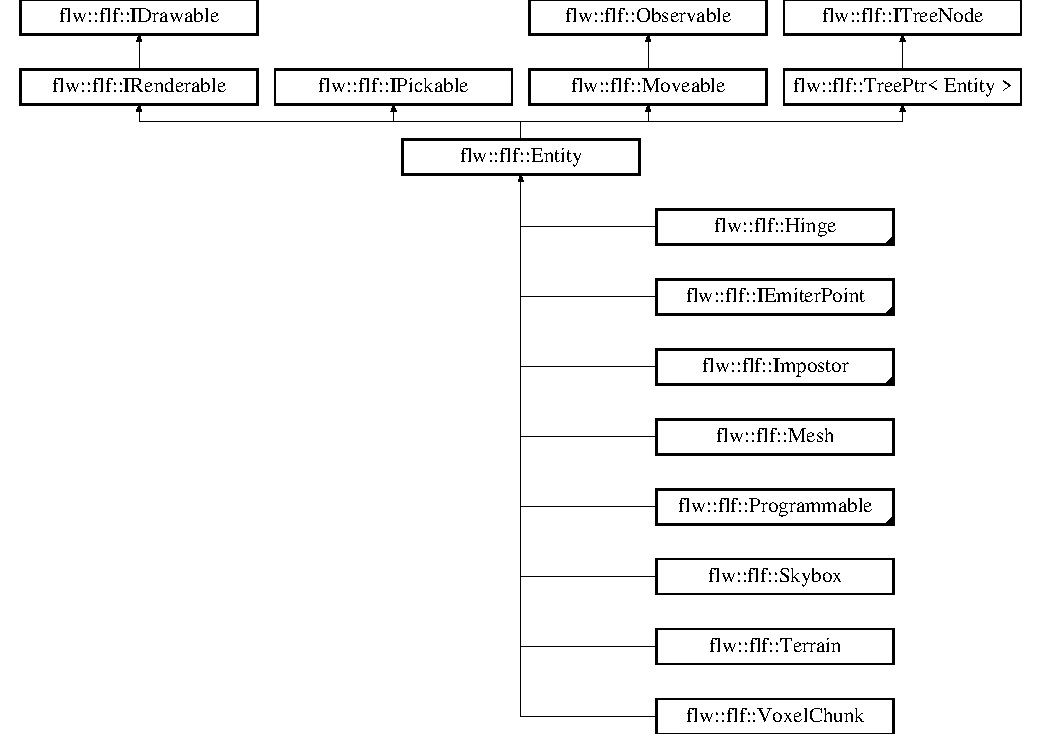
\includegraphics[height=9.871795cm]{classflw_1_1flf_1_1Entity}
\end{center}
\end{figure}
\subsection*{Public Member Functions}
\begin{DoxyCompactItemize}
\item 
{\bfseries Entity} (glm\+::vec3 translation=glm\+::vec3(0.\+0), glm\+::quat orientation=glm\+::quat(1.\+0, 0.\+0, 0.\+0, 0.\+0))\hypertarget{classflw_1_1flf_1_1Entity_ae0bd5d55ad76477802d3976977060e67}{}\label{classflw_1_1flf_1_1Entity_ae0bd5d55ad76477802d3976977060e67}

\item 
\hyperlink{classflw_1_1flf_1_1Entity}{Entity} \& {\bfseries operator=} (const \hyperlink{classflw_1_1flf_1_1Entity}{Entity} \&)=default\hypertarget{classflw_1_1flf_1_1Entity_a87a30a1975aaa8ba7711357cb84ab4ea}{}\label{classflw_1_1flf_1_1Entity_a87a30a1975aaa8ba7711357cb84ab4ea}

\item 
{\bfseries Entity} (const \hyperlink{classflw_1_1flf_1_1Entity}{Entity} \&)=default\hypertarget{classflw_1_1flf_1_1Entity_aa8e3547b5d1b23198e95cf032c48cb85}{}\label{classflw_1_1flf_1_1Entity_aa8e3547b5d1b23198e95cf032c48cb85}

\item 
\hyperlink{classflw_1_1flf_1_1Entity}{Entity} \& {\bfseries operator=} (\hyperlink{classflw_1_1flf_1_1Entity}{Entity} \&\&)=default\hypertarget{classflw_1_1flf_1_1Entity_af1f43a2afb4ac8429d92c7e61a479ce0}{}\label{classflw_1_1flf_1_1Entity_af1f43a2afb4ac8429d92c7e61a479ce0}

\item 
{\bfseries Entity} (\hyperlink{classflw_1_1flf_1_1Entity}{Entity} \&\&obj)=default\hypertarget{classflw_1_1flf_1_1Entity_ab1f2f50ada8a35f1270423776b16201a}{}\label{classflw_1_1flf_1_1Entity_ab1f2f50ada8a35f1270423776b16201a}

\item 
G\+Lboolean {\bfseries is\+P\+SC} ()\hypertarget{classflw_1_1flf_1_1Entity_a2109cfa889dcd96c734e4068dfb4fcaa}{}\label{classflw_1_1flf_1_1Entity_a2109cfa889dcd96c734e4068dfb4fcaa}

\item 
G\+Lboolean {\bfseries is\+P\+SR} ()\hypertarget{classflw_1_1flf_1_1Entity_a475e8d05822681f76ebf21c0218ced53}{}\label{classflw_1_1flf_1_1Entity_a475e8d05822681f76ebf21c0218ced53}

\item 
void {\bfseries handle\+Hierarchy\+Event} (\hyperlink{classflw_1_1flf_1_1EventType}{Event\+Type} \&event)\hypertarget{classflw_1_1flf_1_1Entity_a6f237d03f2e2ff1fc58741c48649334e}{}\label{classflw_1_1flf_1_1Entity_a6f237d03f2e2ff1fc58741c48649334e}

\item 
glm\+::mat4 {\bfseries get\+Physics\+M\+MC} ()\hypertarget{classflw_1_1flf_1_1Entity_a6a3333d6d3ded22c2e3f3cfbcf657d69}{}\label{classflw_1_1flf_1_1Entity_a6a3333d6d3ded22c2e3f3cfbcf657d69}

\item 
void {\bfseries set\+Transformation} (glm\+::mat4 model\+Matrix)\hypertarget{classflw_1_1flf_1_1Entity_a21f8d43b4c42ea9082aecf795a3cecba}{}\label{classflw_1_1flf_1_1Entity_a21f8d43b4c42ea9082aecf795a3cecba}

\item 
void {\bfseries attach\+Hierarchy\+Callback} (pu\+Callback \&\&callback)\hypertarget{classflw_1_1flf_1_1Entity_ae13f1924e429aa49a39b25609ff2ad47}{}\label{classflw_1_1flf_1_1Entity_ae13f1924e429aa49a39b25609ff2ad47}

\item 
void {\bfseries detach\+Hierarchy\+Callback} (\hyperlink{classflw_1_1flf_1_1Callback}{Callback} $\ast$callback)\hypertarget{classflw_1_1flf_1_1Entity_a377051ff8a193e62c315b7b83f5884f2}{}\label{classflw_1_1flf_1_1Entity_a377051ff8a193e62c315b7b83f5884f2}

\item 
void {\bfseries update\+Matrix\+Tree} ()\hypertarget{classflw_1_1flf_1_1Entity_a1a155562e5efcb4523ba78c9f817fafb}{}\label{classflw_1_1flf_1_1Entity_a1a155562e5efcb4523ba78c9f817fafb}

\item 
void {\bfseries update\+Parent\+Matrix} (glm\+::mat4 \&parent)\hypertarget{classflw_1_1flf_1_1Entity_a7296824e646e0d2c4918f258c8af68ed}{}\label{classflw_1_1flf_1_1Entity_a7296824e646e0d2c4918f258c8af68ed}

\item 
void {\bfseries update\+Parent\+Rotation} (glm\+::quat \&rotation)\hypertarget{classflw_1_1flf_1_1Entity_abfb12e4454297961e8345dc70eba43f6}{}\label{classflw_1_1flf_1_1Entity_abfb12e4454297961e8345dc70eba43f6}

\item 
void {\bfseries pick} (glm\+::vec3 color) override\hypertarget{classflw_1_1flf_1_1Entity_aabe261a3cbe923400f5b591e6c2dd782}{}\label{classflw_1_1flf_1_1Entity_aabe261a3cbe923400f5b591e6c2dd782}

\item 
void {\bfseries unpick} () override\hypertarget{classflw_1_1flf_1_1Entity_a96099d66fce38fb7b4b98988d95dda21}{}\label{classflw_1_1flf_1_1Entity_a96099d66fce38fb7b4b98988d95dda21}

\item 
virtual void {\bfseries on\+Picked} () override\hypertarget{classflw_1_1flf_1_1Entity_ac5ac6008e71514da1a33784ad5720ffd}{}\label{classflw_1_1flf_1_1Entity_ac5ac6008e71514da1a33784ad5720ffd}

\item 
virtual void {\bfseries on\+Unpicked} () override\hypertarget{classflw_1_1flf_1_1Entity_aff51141b0c24382055de2eb39b289627}{}\label{classflw_1_1flf_1_1Entity_aff51141b0c24382055de2eb39b289627}

\item 
virtual void {\bfseries draw} (\hyperlink{classflw_1_1flf_1_1ICamera}{I\+Camera} \&camera) override\hypertarget{classflw_1_1flf_1_1Entity_aee49157914b8dc708b4c42bd4ad07073}{}\label{classflw_1_1flf_1_1Entity_aee49157914b8dc708b4c42bd4ad07073}

\item 
virtual void {\bfseries draw\+P\+B\+RP} (\hyperlink{classflw_1_1flf_1_1ICamera}{I\+Camera} \&camera) override\hypertarget{classflw_1_1flf_1_1Entity_a9f77adfda64f405f9975299f4ff75c52}{}\label{classflw_1_1flf_1_1Entity_a9f77adfda64f405f9975299f4ff75c52}

\item 
virtual void {\bfseries draw\+DR} (\hyperlink{classflw_1_1flf_1_1ICamera}{I\+Camera} \&camera) override\hypertarget{classflw_1_1flf_1_1Entity_a83776205205468756486576ee677a31f}{}\label{classflw_1_1flf_1_1Entity_a83776205205468756486576ee677a31f}

\item 
virtual void {\bfseries draw\+Depth} (\hyperlink{classflw_1_1flf_1_1ICamera}{I\+Camera} \&camera) override\hypertarget{classflw_1_1flf_1_1Entity_a62a7675c097053e9906caec2d11d9cb3}{}\label{classflw_1_1flf_1_1Entity_a62a7675c097053e9906caec2d11d9cb3}

\item 
virtual void {\bfseries draw\+Depth\+Color} (\hyperlink{classflw_1_1flf_1_1ICamera}{I\+Camera} \&camera, glm\+::vec3 \&position) override\hypertarget{classflw_1_1flf_1_1Entity_afe8c6cefefc76104ab9b0a5ed80c7443}{}\label{classflw_1_1flf_1_1Entity_afe8c6cefefc76104ab9b0a5ed80c7443}

\item 
virtual void {\bfseries draw\+A\+OG} (\hyperlink{classflw_1_1flf_1_1ICamera}{I\+Camera} \&camera) override\hypertarget{classflw_1_1flf_1_1Entity_aa32e27988fd0434f9b6a2dff1f90335c}{}\label{classflw_1_1flf_1_1Entity_aa32e27988fd0434f9b6a2dff1f90335c}

\item 
virtual void {\bfseries draw\+A\+OC} (\hyperlink{classflw_1_1flf_1_1ICamera}{I\+Camera} \&camera) override\hypertarget{classflw_1_1flf_1_1Entity_a147efc00f87398f5fee13206fdc1c161}{}\label{classflw_1_1flf_1_1Entity_a147efc00f87398f5fee13206fdc1c161}

\item 
virtual void {\bfseries draw\+Occlusion\+Box} (\hyperlink{classflw_1_1flf_1_1ICamera}{I\+Camera} \&camera) override\hypertarget{classflw_1_1flf_1_1Entity_a873a0fa0930c5ac7e1b99011f024a87b}{}\label{classflw_1_1flf_1_1Entity_a873a0fa0930c5ac7e1b99011f024a87b}

\item 
virtual void {\bfseries draw\+Picking} (\hyperlink{classflw_1_1flf_1_1ICamera}{I\+Camera} \&camera) override\hypertarget{classflw_1_1flf_1_1Entity_a58d2d7a158a3f51a507e2c3346c22e91}{}\label{classflw_1_1flf_1_1Entity_a58d2d7a158a3f51a507e2c3346c22e91}

\item 
virtual void {\bfseries update\+Renderer} (\hyperlink{classflw_1_1flf_1_1IRenderer}{I\+Renderer} \&renderer) override\hypertarget{classflw_1_1flf_1_1Entity_a469575479f34a7113331126bd6baee8f}{}\label{classflw_1_1flf_1_1Entity_a469575479f34a7113331126bd6baee8f}

\item 
virtual bool {\bfseries get\+Render\+Item} (\hyperlink{structflw_1_1flf_1_1RenderItem}{Render\+Item} \&item) override\hypertarget{classflw_1_1flf_1_1Entity_a401249745279bc6c62814a50a9ce3ee9}{}\label{classflw_1_1flf_1_1Entity_a401249745279bc6c62814a50a9ce3ee9}

\item 
virtual bool {\bfseries is\+Animated} () const \hypertarget{classflw_1_1flf_1_1Entity_a3f87ebe6d12d0d96339c9e4c81547d30}{}\label{classflw_1_1flf_1_1Entity_a3f87ebe6d12d0d96339c9e4c81547d30}

\item 
virtual void {\bfseries log} () const \hypertarget{classflw_1_1flf_1_1Entity_aea89e4213cc9ee272c188a27cd2360da}{}\label{classflw_1_1flf_1_1Entity_aea89e4213cc9ee272c188a27cd2360da}

\end{DoxyCompactItemize}
\subsection*{Protected Attributes}
\begin{DoxyCompactItemize}
\item 
glm\+::mat4 {\bfseries m\+Physics\+M\+MC}\hypertarget{classflw_1_1flf_1_1Entity_aef9e641dc79bc9dccca0ce13e618ce68}{}\label{classflw_1_1flf_1_1Entity_aef9e641dc79bc9dccca0ce13e618ce68}

\item 
G\+Lboolean {\bfseries m\+Children\+Propagate\+Event}\hypertarget{classflw_1_1flf_1_1Entity_a4a1f8bd96ef1ab91cbcfd146497b7fc3}{}\label{classflw_1_1flf_1_1Entity_a4a1f8bd96ef1ab91cbcfd146497b7fc3}

\item 
G\+Lboolean {\bfseries m\+Parent\+Refresh}\hypertarget{classflw_1_1flf_1_1Entity_aabd5eef30310557a0c7e4d2dbde8b8b1}{}\label{classflw_1_1flf_1_1Entity_aabd5eef30310557a0c7e4d2dbde8b8b1}

\item 
std\+::vector$<$ pu\+Callback $>$ {\bfseries m\+Callbacks\+Hierarchy}\hypertarget{classflw_1_1flf_1_1Entity_a618cff5fcfef2a5f9cae008e7636d9ad}{}\label{classflw_1_1flf_1_1Entity_a618cff5fcfef2a5f9cae008e7636d9ad}

\item 
G\+Lboolean {\bfseries m\+P\+SC}\hypertarget{classflw_1_1flf_1_1Entity_a40c5087118a9ae947f3545833f055801}{}\label{classflw_1_1flf_1_1Entity_a40c5087118a9ae947f3545833f055801}

\item 
G\+Lboolean {\bfseries m\+P\+SR}\hypertarget{classflw_1_1flf_1_1Entity_a459cd19058216cdce6956526db9db0f4}{}\label{classflw_1_1flf_1_1Entity_a459cd19058216cdce6956526db9db0f4}

\end{DoxyCompactItemize}
\subsection*{Additional Inherited Members}


\subsection{Detailed Description}
Base for all \hyperlink{classflw_1_1flf_1_1Scene}{Scene} nodes. 

The documentation for this class was generated from the following file\+:\begin{DoxyCompactItemize}
\item 
/home/filip/\+Projects/fillwave/inc/fillwave/models/Entity.\+h\end{DoxyCompactItemize}

\hypertarget{classflw_1_1flf_1_1EventType}{}\section{flw\+:\+:flf\+:\+:Event\+Type Class Reference}
\label{classflw_1_1flf_1_1EventType}\index{flw\+::flf\+::\+Event\+Type@{flw\+::flf\+::\+Event\+Type}}


Base class for all events. This class needs only the event type (literally -\/ an enumerator) to initialize. Event type defines by which callback the event will be handled.  




{\ttfamily \#include $<$Event\+Type.\+h$>$}

Inheritance diagram for flw\+:\+:flf\+:\+:Event\+Type\+:\begin{figure}[H]
\begin{center}
\leavevmode
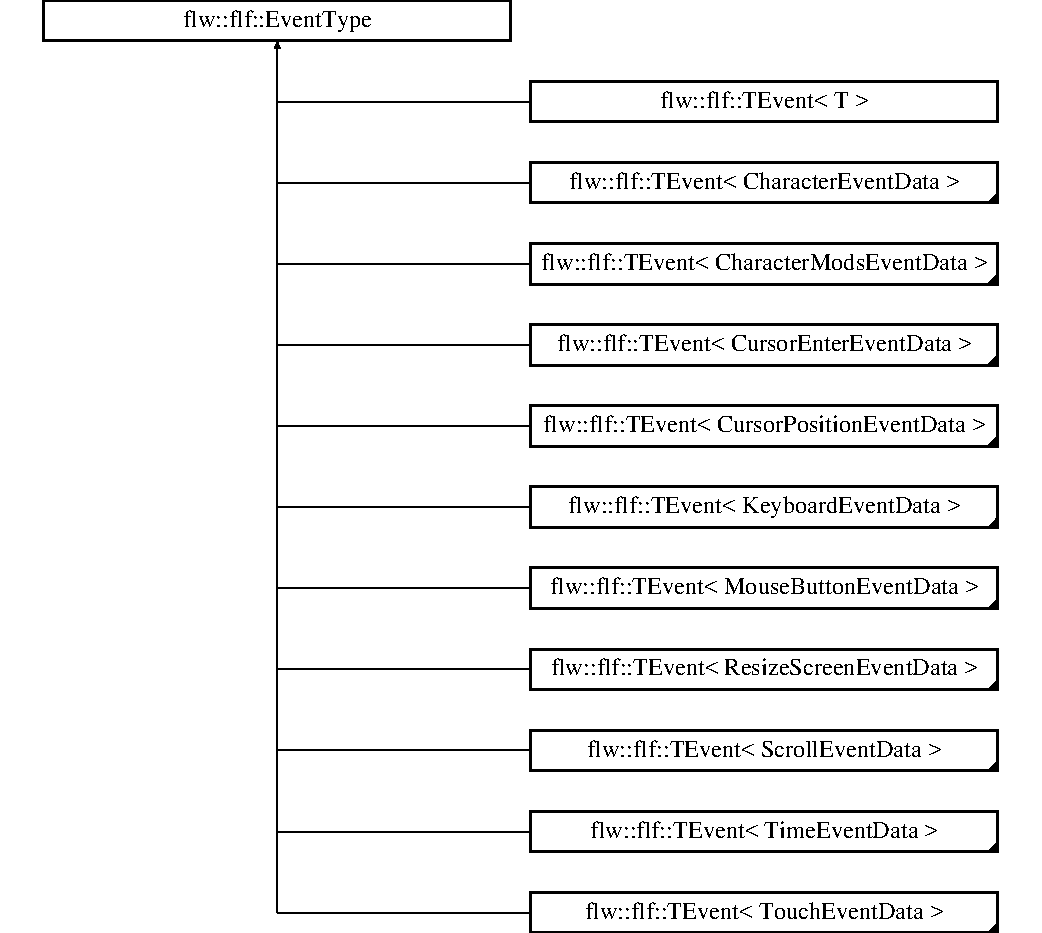
\includegraphics[height=12.000000cm]{classflw_1_1flf_1_1EventType}
\end{center}
\end{figure}
\subsection*{Public Member Functions}
\begin{DoxyCompactItemize}
\item 
{\bfseries Event\+Type} (e\+Event\+Type type)\hypertarget{classflw_1_1flf_1_1EventType_a9965ef6f0b75517dda7f87e00beae5d0}{}\label{classflw_1_1flf_1_1EventType_a9965ef6f0b75517dda7f87e00beae5d0}

\item 
e\+Event\+Type {\bfseries get\+Type} ()\hypertarget{classflw_1_1flf_1_1EventType_a5ac577de1d726b1f47b5c08a9f597438}{}\label{classflw_1_1flf_1_1EventType_a5ac577de1d726b1f47b5c08a9f597438}

\end{DoxyCompactItemize}


\subsection{Detailed Description}
Base class for all events. This class needs only the event type (literally -\/ an enumerator) to initialize. Event type defines by which callback the event will be handled. 

The documentation for this class was generated from the following file\+:\begin{DoxyCompactItemize}
\item 
/home/filip/\+Projects/fillwave/inc/fillwave/actions/events/Event\+Type.\+h\end{DoxyCompactItemize}

\hypertarget{classflw_1_1flf_1_1ExceptionFillwave}{}\section{flw\+:\+:flf\+:\+:Exception\+Fillwave Class Reference}
\label{classflw_1_1flf_1_1ExceptionFillwave}\index{flw\+::flf\+::\+Exception\+Fillwave@{flw\+::flf\+::\+Exception\+Fillwave}}


Not used.  




{\ttfamily \#include $<$Exception\+Fillwave.\+h$>$}

Inheritance diagram for flw\+:\+:flf\+:\+:Exception\+Fillwave\+:\begin{figure}[H]
\begin{center}
\leavevmode
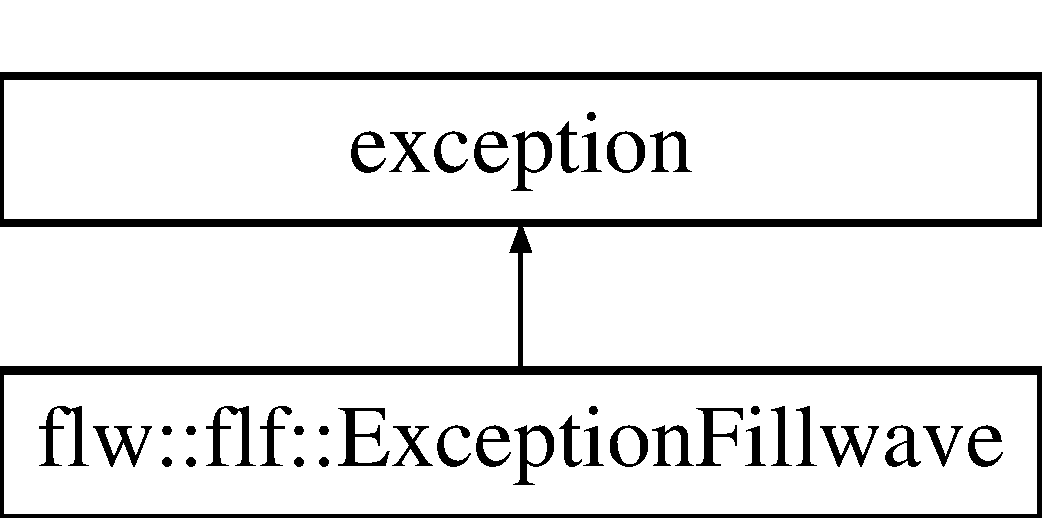
\includegraphics[height=2.000000cm]{classflw_1_1flf_1_1ExceptionFillwave}
\end{center}
\end{figure}
\subsection*{Public Member Functions}
\begin{DoxyCompactItemize}
\item 
\mbox{\Hypertarget{classflw_1_1flf_1_1ExceptionFillwave_a342a4c65c3bf2b3cff8d0d161e637912}\label{classflw_1_1flf_1_1ExceptionFillwave_a342a4c65c3bf2b3cff8d0d161e637912}} 
{\bfseries Exception\+Fillwave} (const std\+::string \&why)
\item 
\mbox{\Hypertarget{classflw_1_1flf_1_1ExceptionFillwave_ae62574fc52459015e779cc7026f965ce}\label{classflw_1_1flf_1_1ExceptionFillwave_ae62574fc52459015e779cc7026f965ce}} 
virtual const char $\ast$ {\bfseries what} () const  throw ()
\end{DoxyCompactItemize}


\subsection{Detailed Description}
Not used. 

The documentation for this class was generated from the following file\+:\begin{DoxyCompactItemize}
\item 
/home/filip/projects/fillwave/inc/fillwave/common/Exception\+Fillwave.\+h\end{DoxyCompactItemize}

\hypertarget{structflw_1_1flc_1_1FaceBasic}{}\section{flw\+:\+:flc\+:\+:Face\+Basic Struct Reference}
\label{structflw_1_1flc_1_1FaceBasic}\index{flw\+::flc\+::\+Face\+Basic@{flw\+::flc\+::\+Face\+Basic}}


Stores the face data for geometry built on Vertex Basic.  




{\ttfamily \#include $<$Vertex\+Buffer\+Basic.\+h$>$}

\subsection*{Public Attributes}
\begin{DoxyCompactItemize}
\item 
\hyperlink{structflw_1_1flc_1_1VertexBasic}{flc\+::\+Vertex\+Basic} {\bfseries vertices} \mbox{[}3\mbox{]}\hypertarget{structflw_1_1flc_1_1FaceBasic_a38791ec533656c6001d311132000774b}{}\label{structflw_1_1flc_1_1FaceBasic_a38791ec533656c6001d311132000774b}

\end{DoxyCompactItemize}


\subsection{Detailed Description}
Stores the face data for geometry built on Vertex Basic. 

The documentation for this struct was generated from the following file\+:\begin{DoxyCompactItemize}
\item 
/home/filip/\+Projects/fillwave/inc/fillwave/core/buffers/Vertex\+Buffer\+Basic.\+h\end{DoxyCompactItemize}

\hypertarget{classflw_1_1flc_1_1Fence}{}\section{flw\+:\+:flc\+:\+:Fence Class Reference}
\label{classflw_1_1flc_1_1Fence}\index{flw\+::flc\+::\+Fence@{flw\+::flc\+::\+Fence}}


Sets a fence for a gpu to wait.  




{\ttfamily \#include $<$Fence.\+h$>$}

\subsection*{Public Member Functions}
\begin{DoxyCompactItemize}
\item 
\mbox{\Hypertarget{classflw_1_1flc_1_1Fence_a431a609115c5a2965b7e778897c7df7a}\label{classflw_1_1flc_1_1Fence_a431a609115c5a2965b7e778897c7df7a}} 
{\bfseries Fence} (G\+Lenum target=G\+L\+\_\+\+S\+Y\+N\+C\+\_\+\+G\+P\+U\+\_\+\+C\+O\+M\+M\+A\+N\+D\+S\+\_\+\+C\+O\+M\+P\+L\+E\+TE)
\item 
\mbox{\Hypertarget{classflw_1_1flc_1_1Fence_a0837c669bd405ced5c75fe2781136819}\label{classflw_1_1flc_1_1Fence_a0837c669bd405ced5c75fe2781136819}} 
void {\bfseries wait} (unsigned long long timeout\+Specifier=G\+L\+\_\+\+T\+I\+M\+E\+O\+U\+T\+\_\+\+I\+G\+N\+O\+R\+ED) const
\end{DoxyCompactItemize}


\subsection{Detailed Description}
Sets a fence for a gpu to wait. 

The documentation for this class was generated from the following file\+:\begin{DoxyCompactItemize}
\item 
/home/filip/projects/fillwave/inc/fillwave/core/pipeline/Fence.\+h\end{DoxyCompactItemize}

\hypertarget{classflw_1_1flf_1_1FileLoader}{}\section{flw\+:\+:flf\+:\+:File\+Loader Class Reference}
\label{classflw_1_1flf_1_1FileLoader}\index{flw\+::flf\+::\+File\+Loader@{flw\+::flf\+::\+File\+Loader}}


Loads files.  




{\ttfamily \#include $<$File\+Loader.\+h$>$}

\subsection*{Public Member Functions}
\begin{DoxyCompactItemize}
\item 
\mbox{\Hypertarget{classflw_1_1flf_1_1FileLoader_a600a5a31f5658122a037e464f59010da}\label{classflw_1_1flf_1_1FileLoader_a600a5a31f5658122a037e464f59010da}} 
{\bfseries File\+Loader} (const std\+::string \&root\+Path)
\item 
\mbox{\Hypertarget{classflw_1_1flf_1_1FileLoader_a9cdf33046f1616a0e75ae1eea9e06448}\label{classflw_1_1flf_1_1FileLoader_a9cdf33046f1616a0e75ae1eea9e06448}} 
std\+::string {\bfseries get\+Root\+Path} (std\+::string file\+Path=\char`\"{}\char`\"{})
\end{DoxyCompactItemize}


\subsection{Detailed Description}
Loads files. 

The documentation for this class was generated from the following file\+:\begin{DoxyCompactItemize}
\item 
/home/filip/projects/fillwave/inc/fillwave/loaders/File\+Loader.\+h\end{DoxyCompactItemize}

\hypertarget{classflw_1_1flf_1_1Finishable}{}\section{flw\+:\+:flf\+:\+:Finishable Class Reference}
\label{classflw_1_1flf_1_1Finishable}\index{flw\+::flf\+::\+Finishable@{flw\+::flf\+::\+Finishable}}


Base for every finishable callback.  




{\ttfamily \#include $<$Finishable.\+h$>$}

Inheritance diagram for flw\+:\+:flf\+:\+:Finishable\+:\begin{figure}[H]
\begin{center}
\leavevmode
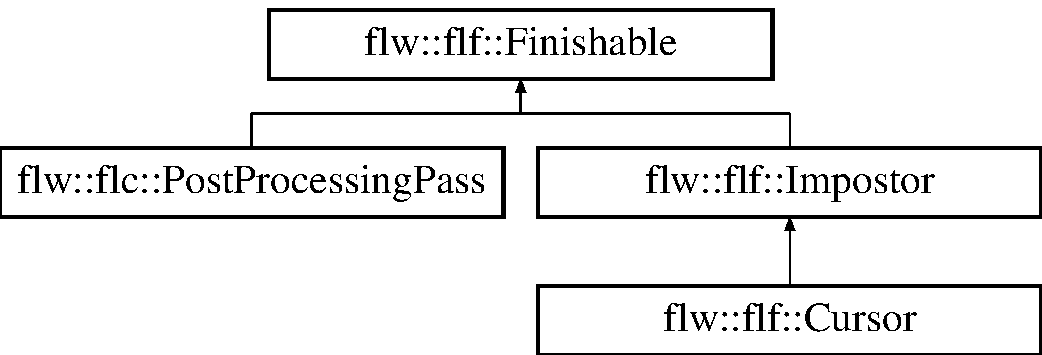
\includegraphics[height=3.000000cm]{classflw_1_1flf_1_1Finishable}
\end{center}
\end{figure}
\subsection*{Public Member Functions}
\begin{DoxyCompactItemize}
\item 
\mbox{\Hypertarget{classflw_1_1flf_1_1Finishable_a167dd981e22d9450aefdaf905cfae8bb}\label{classflw_1_1flf_1_1Finishable_a167dd981e22d9450aefdaf905cfae8bb}} 
{\bfseries Finishable} (float time\+To\+Finish)
\item 
\mbox{\Hypertarget{classflw_1_1flf_1_1Finishable_af3a1125b567dcb2d5c0b4f3ce5246961}\label{classflw_1_1flf_1_1Finishable_af3a1125b567dcb2d5c0b4f3ce5246961}} 
void {\bfseries check\+Time} (float time\+Passed)
\item 
\mbox{\Hypertarget{classflw_1_1flf_1_1Finishable_a298ade78c1c08c4832689ef8a09df3cc}\label{classflw_1_1flf_1_1Finishable_a298ade78c1c08c4832689ef8a09df3cc}} 
float {\bfseries get\+Percentage\+Done} () const
\item 
\mbox{\Hypertarget{classflw_1_1flf_1_1Finishable_ae050528989ddef860d457264b014d869}\label{classflw_1_1flf_1_1Finishable_ae050528989ddef860d457264b014d869}} 
void {\bfseries finish} ()
\item 
\mbox{\Hypertarget{classflw_1_1flf_1_1Finishable_a8f0662da7f8881ce02f9211ba68d4995}\label{classflw_1_1flf_1_1Finishable_a8f0662da7f8881ce02f9211ba68d4995}} 
void {\bfseries reset} ()
\item 
\mbox{\Hypertarget{classflw_1_1flf_1_1Finishable_a4f5caae7c8be0f9b275fcc93ad9e5428}\label{classflw_1_1flf_1_1Finishable_a4f5caae7c8be0f9b275fcc93ad9e5428}} 
bool {\bfseries is\+Finished} () const
\end{DoxyCompactItemize}
\subsection*{Protected Attributes}
\begin{DoxyCompactItemize}
\item 
\mbox{\Hypertarget{classflw_1_1flf_1_1Finishable_a7ece5edd33fd456e1845ca7c9e209882}\label{classflw_1_1flf_1_1Finishable_a7ece5edd33fd456e1845ca7c9e209882}} 
bool {\bfseries m\+Finished}
\item 
\mbox{\Hypertarget{classflw_1_1flf_1_1Finishable_a4c1792287327a12b3089faef3bae7a4f}\label{classflw_1_1flf_1_1Finishable_a4c1792287327a12b3089faef3bae7a4f}} 
float {\bfseries m\+Time\+To\+Finish}
\item 
\mbox{\Hypertarget{classflw_1_1flf_1_1Finishable_a51e6bc00dfe9b1a7726e7f6fde2dc9ce}\label{classflw_1_1flf_1_1Finishable_a51e6bc00dfe9b1a7726e7f6fde2dc9ce}} 
float {\bfseries m\+Time\+Passed}
\item 
\mbox{\Hypertarget{classflw_1_1flf_1_1Finishable_a8da70d226a3aa1663a328aa4eaefbd1d}\label{classflw_1_1flf_1_1Finishable_a8da70d226a3aa1663a328aa4eaefbd1d}} 
float {\bfseries m\+Percentage\+Done}
\end{DoxyCompactItemize}


\subsection{Detailed Description}
Base for every finishable callback. 

The documentation for this class was generated from the following file\+:\begin{DoxyCompactItemize}
\item 
/home/filip/projects/fillwave/inc/fillwave/common/Finishable.\+h\end{DoxyCompactItemize}

\hypertarget{classflw_1_1flf_1_1Fog}{}\section{flw\+:\+:flf\+:\+:Fog Class Reference}
\label{classflw_1_1flf_1_1Fog}\index{flw\+::flf\+::\+Fog@{flw\+::flf\+::\+Fog}}


Effect to create a fog.  




{\ttfamily \#include $<$Fog.\+h$>$}

Inheritance diagram for flw\+:\+:flf\+:\+:Fog\+:\begin{figure}[H]
\begin{center}
\leavevmode
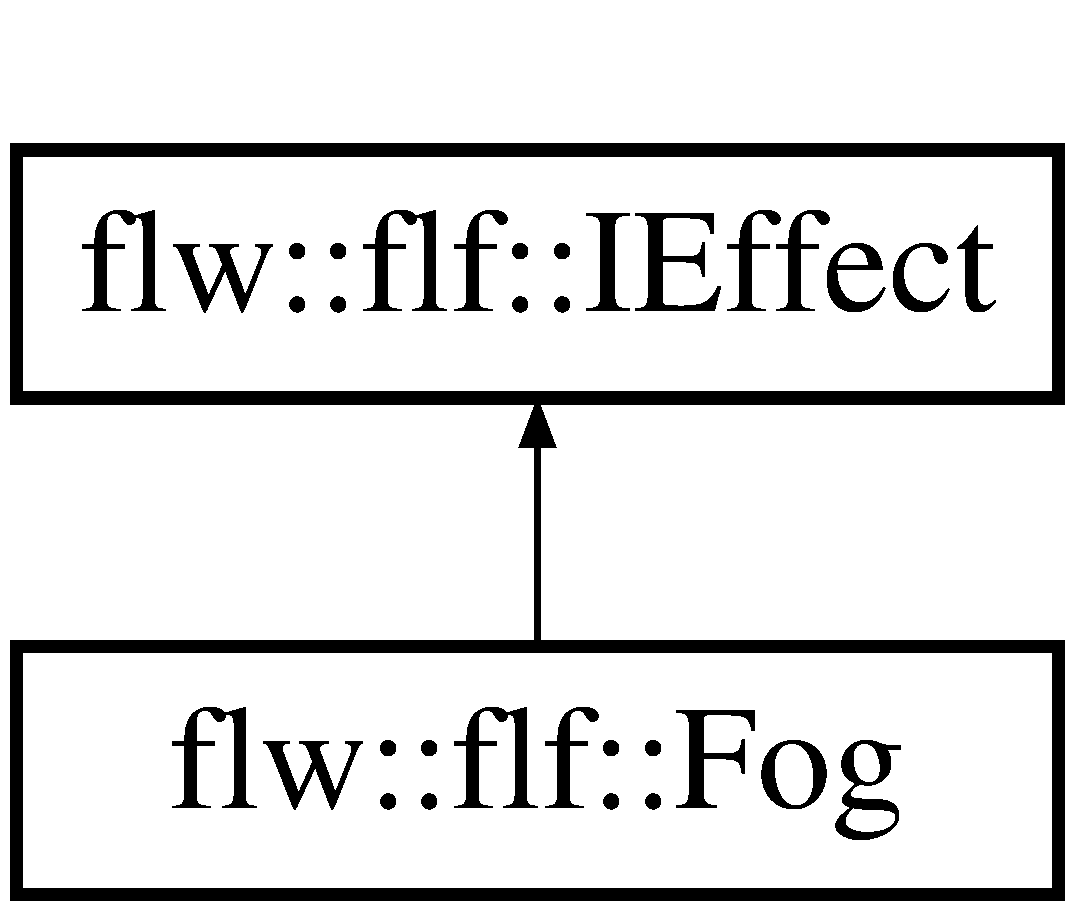
\includegraphics[height=2.000000cm]{classflw_1_1flf_1_1Fog}
\end{center}
\end{figure}
\subsection*{Public Member Functions}
\begin{DoxyCompactItemize}
\item 
{\bfseries Fog} (glm\+::vec3 colour=glm\+::vec3(0.\+1f, 0.\+1f, 0.\+1f), G\+Lfloat near=0.\+1f, G\+Lfloat far=20.\+0f)\hypertarget{classflw_1_1flf_1_1Fog_a2bfdacc7a2c9b4320af0ad5dbe2989e8}{}\label{classflw_1_1flf_1_1Fog_a2bfdacc7a2c9b4320af0ad5dbe2989e8}

\item 
glm\+::vec3 {\bfseries get\+Colour} ()\hypertarget{classflw_1_1flf_1_1Fog_ae70d98849f2f0d569eb79177cfb00c1c}{}\label{classflw_1_1flf_1_1Fog_ae70d98849f2f0d569eb79177cfb00c1c}

\item 
G\+Lfloat {\bfseries get\+Near\+Distance} ()\hypertarget{classflw_1_1flf_1_1Fog_acdc4eec649e8e103e826b27d078b9b78}{}\label{classflw_1_1flf_1_1Fog_acdc4eec649e8e103e826b27d078b9b78}

\item 
G\+Lfloat {\bfseries get\+Far\+Distance} ()\hypertarget{classflw_1_1flf_1_1Fog_a47fa640d7ac15c6f00865fb65d9200c5}{}\label{classflw_1_1flf_1_1Fog_a47fa640d7ac15c6f00865fb65d9200c5}

\item 
void {\bfseries set\+Colour} (glm\+::vec3 colour)\hypertarget{classflw_1_1flf_1_1Fog_a878c0fe57d32ed19b953a2b80049df51}{}\label{classflw_1_1flf_1_1Fog_a878c0fe57d32ed19b953a2b80049df51}

\item 
void {\bfseries set\+Near\+Distance} (G\+Lfloat a\+Near)\hypertarget{classflw_1_1flf_1_1Fog_a92734a69fca7b000d3656642971624c4}{}\label{classflw_1_1flf_1_1Fog_a92734a69fca7b000d3656642971624c4}

\item 
void {\bfseries set\+Far\+Distance} (G\+Lfloat a\+Far)\hypertarget{classflw_1_1flf_1_1Fog_abcd9c04cd7c8a793e63409ee7a8ba82a}{}\label{classflw_1_1flf_1_1Fog_abcd9c04cd7c8a793e63409ee7a8ba82a}

\item 
void \hyperlink{classflw_1_1flf_1_1Fog_a0d426e670e2b976601144e28c7dc5a48}{pre\+Draw\+Action} (\hyperlink{classflw_1_1flc_1_1Program}{flc\+::\+Program} $\ast$program) override
\begin{DoxyCompactList}\small\item\em virtual\+: defines action to be done just before the draw. \end{DoxyCompactList}\item 
void \hyperlink{classflw_1_1flf_1_1Fog_a23da383300538478081e23277bcca4fa}{post\+Draw\+Action} (\hyperlink{classflw_1_1flc_1_1Program}{flc\+::\+Program} $\ast$program) override
\begin{DoxyCompactList}\small\item\em virtual\+: defines action to be done just after the draw. \end{DoxyCompactList}\item 
void \hyperlink{classflw_1_1flf_1_1Fog_ab1b33ed568e679c51f24937db7ffd45c}{stop\+Action} (\hyperlink{classflw_1_1flc_1_1Program}{flc\+::\+Program} $\ast$program) override
\begin{DoxyCompactList}\small\item\em virtual\+: defines action to be done when the effect is stopped. \end{DoxyCompactList}\item 
void \hyperlink{classflw_1_1flf_1_1Fog_a12acc2ae25d54721648265aa863c8b1e}{start\+Action} (\hyperlink{classflw_1_1flc_1_1Program}{flc\+::\+Program} $\ast$program) override
\begin{DoxyCompactList}\small\item\em virtual\+: defines action to be done when the effect is started. \end{DoxyCompactList}\end{DoxyCompactItemize}


\subsection{Detailed Description}
Effect to create a fog. 

\subsection{Member Function Documentation}
\index{flw\+::flf\+::\+Fog@{flw\+::flf\+::\+Fog}!post\+Draw\+Action@{post\+Draw\+Action}}
\index{post\+Draw\+Action@{post\+Draw\+Action}!flw\+::flf\+::\+Fog@{flw\+::flf\+::\+Fog}}
\subsubsection[{\texorpdfstring{post\+Draw\+Action(flc\+::\+Program $\ast$program) override}{postDrawAction(flc::Program *program) override}}]{\setlength{\rightskip}{0pt plus 5cm}void flw\+::flf\+::\+Fog\+::post\+Draw\+Action (
\begin{DoxyParamCaption}
\item[{{\bf flc\+::\+Program} $\ast$}]{program}
\end{DoxyParamCaption}
)\hspace{0.3cm}{\ttfamily [override]}, {\ttfamily [virtual]}}\hypertarget{classflw_1_1flf_1_1Fog_a23da383300538478081e23277bcca4fa}{}\label{classflw_1_1flf_1_1Fog_a23da383300538478081e23277bcca4fa}


virtual\+: defines action to be done just after the draw. 

post\+Draw\+Action 

Implements \hyperlink{classflw_1_1flf_1_1IEffect_a6bb11d90e7e4da057ca398bd8c61208a}{flw\+::flf\+::\+I\+Effect}.

\index{flw\+::flf\+::\+Fog@{flw\+::flf\+::\+Fog}!pre\+Draw\+Action@{pre\+Draw\+Action}}
\index{pre\+Draw\+Action@{pre\+Draw\+Action}!flw\+::flf\+::\+Fog@{flw\+::flf\+::\+Fog}}
\subsubsection[{\texorpdfstring{pre\+Draw\+Action(flc\+::\+Program $\ast$program) override}{preDrawAction(flc::Program *program) override}}]{\setlength{\rightskip}{0pt plus 5cm}void flw\+::flf\+::\+Fog\+::pre\+Draw\+Action (
\begin{DoxyParamCaption}
\item[{{\bf flc\+::\+Program} $\ast$}]{program}
\end{DoxyParamCaption}
)\hspace{0.3cm}{\ttfamily [override]}, {\ttfamily [virtual]}}\hypertarget{classflw_1_1flf_1_1Fog_a0d426e670e2b976601144e28c7dc5a48}{}\label{classflw_1_1flf_1_1Fog_a0d426e670e2b976601144e28c7dc5a48}


virtual\+: defines action to be done just before the draw. 

pre\+Draw\+Action 

Implements \hyperlink{classflw_1_1flf_1_1IEffect_ae65eed21e40a226c7739d3c5dedd9e50}{flw\+::flf\+::\+I\+Effect}.

\index{flw\+::flf\+::\+Fog@{flw\+::flf\+::\+Fog}!start\+Action@{start\+Action}}
\index{start\+Action@{start\+Action}!flw\+::flf\+::\+Fog@{flw\+::flf\+::\+Fog}}
\subsubsection[{\texorpdfstring{start\+Action(flc\+::\+Program $\ast$program) override}{startAction(flc::Program *program) override}}]{\setlength{\rightskip}{0pt plus 5cm}void flw\+::flf\+::\+Fog\+::start\+Action (
\begin{DoxyParamCaption}
\item[{{\bf flc\+::\+Program} $\ast$}]{program}
\end{DoxyParamCaption}
)\hspace{0.3cm}{\ttfamily [override]}, {\ttfamily [virtual]}}\hypertarget{classflw_1_1flf_1_1Fog_a12acc2ae25d54721648265aa863c8b1e}{}\label{classflw_1_1flf_1_1Fog_a12acc2ae25d54721648265aa863c8b1e}


virtual\+: defines action to be done when the effect is started. 

start\+Action 

Implements \hyperlink{classflw_1_1flf_1_1IEffect_afc7cec9080d135ed264b08a90c7b94e9}{flw\+::flf\+::\+I\+Effect}.

\index{flw\+::flf\+::\+Fog@{flw\+::flf\+::\+Fog}!stop\+Action@{stop\+Action}}
\index{stop\+Action@{stop\+Action}!flw\+::flf\+::\+Fog@{flw\+::flf\+::\+Fog}}
\subsubsection[{\texorpdfstring{stop\+Action(flc\+::\+Program $\ast$program) override}{stopAction(flc::Program *program) override}}]{\setlength{\rightskip}{0pt plus 5cm}void flw\+::flf\+::\+Fog\+::stop\+Action (
\begin{DoxyParamCaption}
\item[{{\bf flc\+::\+Program} $\ast$}]{program}
\end{DoxyParamCaption}
)\hspace{0.3cm}{\ttfamily [override]}, {\ttfamily [virtual]}}\hypertarget{classflw_1_1flf_1_1Fog_ab1b33ed568e679c51f24937db7ffd45c}{}\label{classflw_1_1flf_1_1Fog_ab1b33ed568e679c51f24937db7ffd45c}


virtual\+: defines action to be done when the effect is stopped. 

stop\+Action 

Implements \hyperlink{classflw_1_1flf_1_1IEffect_a1a03eaf63a9d4edbd8764540d2d4133c}{flw\+::flf\+::\+I\+Effect}.



The documentation for this class was generated from the following file\+:\begin{DoxyCompactItemize}
\item 
/home/filip/\+Projects/fillwave/inc/fillwave/models/effects/Fog.\+h\end{DoxyCompactItemize}

\hypertarget{classflw_1_1flf_1_1FontLoader}{}\section{flw\+:\+:flf\+:\+:Font\+Loader Class Reference}
\label{classflw_1_1flf_1_1FontLoader}\index{flw\+::flf\+::\+Font\+Loader@{flw\+::flf\+::\+Font\+Loader}}


Loads fonts fromttf files.  




{\ttfamily \#include $<$Font\+Loader.\+h$>$}

\subsection*{Public Member Functions}
\begin{DoxyCompactItemize}
\item 
\mbox{\Hypertarget{classflw_1_1flf_1_1FontLoader_ab749fb5cf17cc2ee89072fe1295e72ba}\label{classflw_1_1flf_1_1FontLoader_ab749fb5cf17cc2ee89072fe1295e72ba}} 
void {\bfseries load} (std\+::string name)
\end{DoxyCompactItemize}


\subsection{Detailed Description}
Loads fonts fromttf files. 

The documentation for this class was generated from the following file\+:\begin{DoxyCompactItemize}
\item 
/home/filip/projects/fillwave/inc/fillwave/loaders/Font\+Loader.\+h\end{DoxyCompactItemize}

\hypertarget{classflw_1_1flf_1_1FPSCallback}{}\section{flw\+:\+:flf\+:\+:F\+P\+S\+Callback Class Reference}
\label{classflw_1_1flf_1_1FPSCallback}\index{flw\+::flf\+::\+F\+P\+S\+Callback@{flw\+::flf\+::\+F\+P\+S\+Callback}}


Item\+Callback to display and refresh F\+PS as a renderable text.  




{\ttfamily \#include $<$F\+P\+S\+Callback.\+h$>$}

Inheritance diagram for flw\+:\+:flf\+:\+:F\+P\+S\+Callback\+:\begin{figure}[H]
\begin{center}
\leavevmode
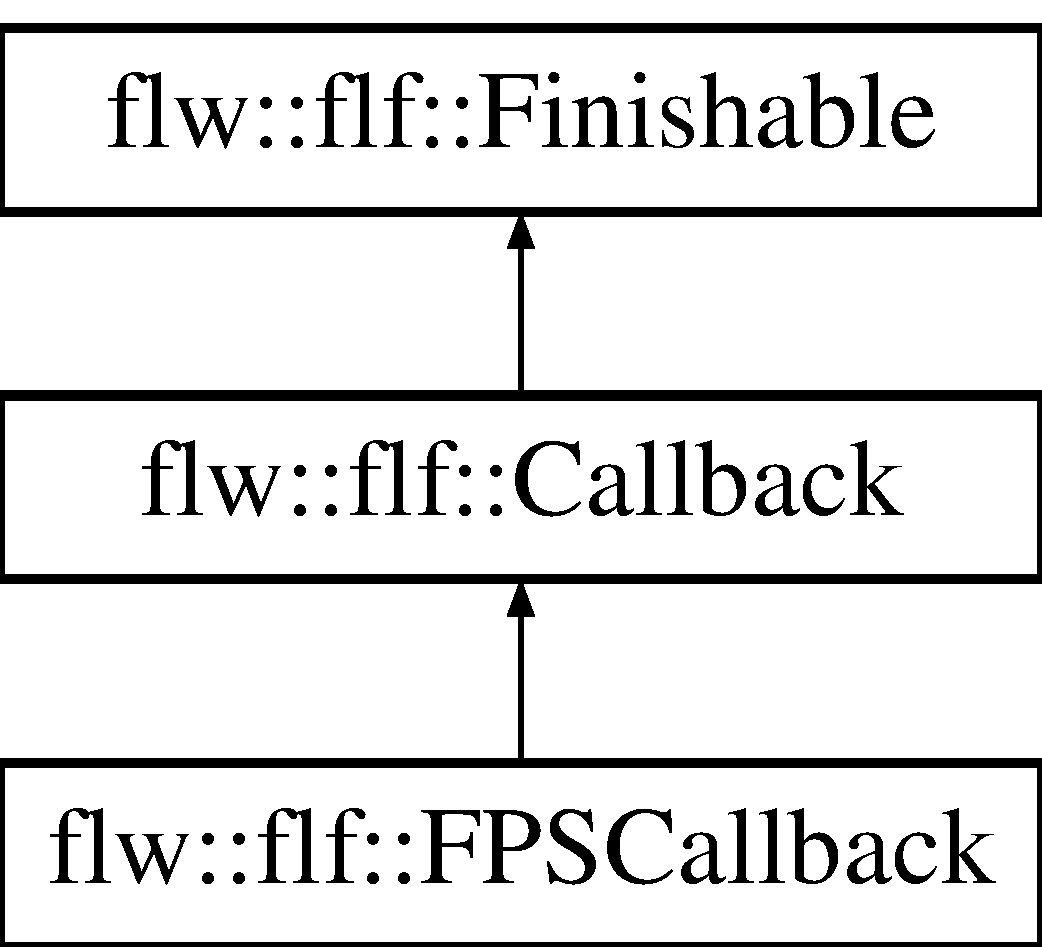
\includegraphics[height=3.000000cm]{classflw_1_1flf_1_1FPSCallback}
\end{center}
\end{figure}
\subsection*{Public Member Functions}
\begin{DoxyCompactItemize}
\item 
{\bfseries F\+P\+S\+Callback} (\hyperlink{classflw_1_1Engine}{Engine} $\ast$engine, p\+Text text)\hypertarget{classflw_1_1flf_1_1FPSCallback_acac067ca5228b11a0037bac1f795977a}{}\label{classflw_1_1flf_1_1FPSCallback_acac067ca5228b11a0037bac1f795977a}

\item 
void {\bfseries perform} (\hyperlink{classflw_1_1flf_1_1EventType}{Event\+Type} \&event)\hypertarget{classflw_1_1flf_1_1FPSCallback_a2cdbd06e7b0f63958ed32763ef9fd41d}{}\label{classflw_1_1flf_1_1FPSCallback_a2cdbd06e7b0f63958ed32763ef9fd41d}

\end{DoxyCompactItemize}
\subsection*{Additional Inherited Members}


\subsection{Detailed Description}
Item\+Callback to display and refresh F\+PS as a renderable text. 

The documentation for this class was generated from the following file\+:\begin{DoxyCompactItemize}
\item 
/home/filip/\+Projects/fillwave/inc/fillwave/actions/callbacks/F\+P\+S\+Callback.\+h\end{DoxyCompactItemize}

\hypertarget{classflw_1_1flc_1_1Framebuffer}{}\section{flw\+:\+:flc\+:\+:Framebuffer Class Reference}
\label{classflw_1_1flc_1_1Framebuffer}\index{flw\+::flc\+::\+Framebuffer@{flw\+::flc\+::\+Framebuffer}}


Framebuffer\+Object -\/ FO.  




{\ttfamily \#include $<$Framebuffer.\+h$>$}

Inheritance diagram for flw\+:\+:flc\+:\+:Framebuffer\+:\begin{figure}[H]
\begin{center}
\leavevmode
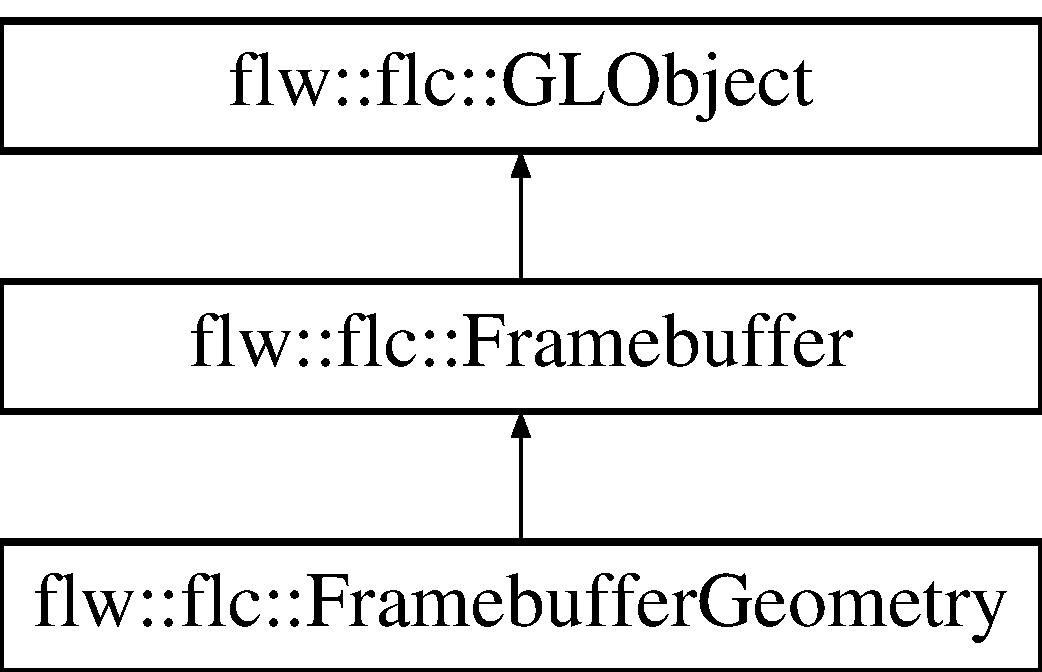
\includegraphics[height=3.000000cm]{classflw_1_1flc_1_1Framebuffer}
\end{center}
\end{figure}
\subsection*{Public Member Functions}
\begin{DoxyCompactItemize}
\item 
\mbox{\Hypertarget{classflw_1_1flc_1_1Framebuffer_a26f65451d5e89e0fedd6e561e4d52cff}\label{classflw_1_1flc_1_1Framebuffer_a26f65451d5e89e0fedd6e561e4d52cff}} 
{\bfseries Framebuffer} (G\+Luint how\+Many=1)
\item 
\mbox{\Hypertarget{classflw_1_1flc_1_1Framebuffer_a38fe5a9625b1af44083931f8bee41a67}\label{classflw_1_1flc_1_1Framebuffer_a38fe5a9625b1af44083931f8bee41a67}} 
void {\bfseries bind} (G\+Luint id=0) const
\item 
\mbox{\Hypertarget{classflw_1_1flc_1_1Framebuffer_a1bc551a6f679db926250460486ed591f}\label{classflw_1_1flc_1_1Framebuffer_a1bc551a6f679db926250460486ed591f}} 
void {\bfseries attach\+Texture2D} (G\+Lenum attachment, G\+Lenum target, G\+Luint texture\+Handle)
\item 
\mbox{\Hypertarget{classflw_1_1flc_1_1Framebuffer_a20cfb02c1ff5841c1a90e58b8fdb1cf1}\label{classflw_1_1flc_1_1Framebuffer_a20cfb02c1ff5841c1a90e58b8fdb1cf1}} 
void {\bfseries attach\+Texture2\+D\+Draw} (G\+Lenum attachment, G\+Lenum target, G\+Luint texture\+Handle)
\item 
\mbox{\Hypertarget{classflw_1_1flc_1_1Framebuffer_a86c62fb48ced666f0725f77fbb77c280}\label{classflw_1_1flc_1_1Framebuffer_a86c62fb48ced666f0725f77fbb77c280}} 
void {\bfseries bind\+For\+Writing} (G\+Luint id=0) const
\item 
\mbox{\Hypertarget{classflw_1_1flc_1_1Framebuffer_a8696d80107cb7cfcaba81066bf085eea}\label{classflw_1_1flc_1_1Framebuffer_a8696d80107cb7cfcaba81066bf085eea}} 
void {\bfseries bind\+For\+Reading} (G\+Luint id=0) const
\item 
\mbox{\Hypertarget{classflw_1_1flc_1_1Framebuffer_a6c4f090bf34b3d50bc6ba3bd642f4448}\label{classflw_1_1flc_1_1Framebuffer_a6c4f090bf34b3d50bc6ba3bd642f4448}} 
void {\bfseries set\+Read\+Color\+Attachment} (G\+Luint attachment\+Color)
\item 
\mbox{\Hypertarget{classflw_1_1flc_1_1Framebuffer_a4c407fdc426e9be189457eb20c6a1f70}\label{classflw_1_1flc_1_1Framebuffer_a4c407fdc426e9be189457eb20c6a1f70}} 
void {\bfseries set\+Read\+Depth\+Attachment} ()
\item 
\mbox{\Hypertarget{classflw_1_1flc_1_1Framebuffer_a1ebc408b16d41bb783768d152b9bf939}\label{classflw_1_1flc_1_1Framebuffer_a1ebc408b16d41bb783768d152b9bf939}} 
virtual void {\bfseries reload} ()
\end{DoxyCompactItemize}
\subsection*{Static Public Member Functions}
\begin{DoxyCompactItemize}
\item 
\mbox{\Hypertarget{classflw_1_1flc_1_1Framebuffer_ab0dab25735dc8694de3c4c05cf0cfedf}\label{classflw_1_1flc_1_1Framebuffer_ab0dab25735dc8694de3c4c05cf0cfedf}} 
static void {\bfseries bind\+Screen\+Framebuffer} ()
\item 
\mbox{\Hypertarget{classflw_1_1flc_1_1Framebuffer_a4f51156591b3b95480621cf3eb424328}\label{classflw_1_1flc_1_1Framebuffer_a4f51156591b3b95480621cf3eb424328}} 
static void {\bfseries bind\+Screen\+Framebuffer\+For\+Reading} ()
\item 
\mbox{\Hypertarget{classflw_1_1flc_1_1Framebuffer_a0e99d4cc1d24e9ae016695ddc524bdd3}\label{classflw_1_1flc_1_1Framebuffer_a0e99d4cc1d24e9ae016695ddc524bdd3}} 
static void {\bfseries bind\+Screen\+Framebuffer\+For\+Writing} ()
\end{DoxyCompactItemize}
\subsection*{Additional Inherited Members}


\subsection{Detailed Description}
Framebuffer\+Object -\/ FO. 

The documentation for this class was generated from the following file\+:\begin{DoxyCompactItemize}
\item 
/home/filip/projects/fillwave/inc/fillwave/core/rendering/Framebuffer.\+h\end{DoxyCompactItemize}

\hypertarget{classflw_1_1flc_1_1FramebufferGeometry}{}\section{flw\+:\+:flc\+:\+:Framebuffer\+Geometry Class Reference}
\label{classflw_1_1flc_1_1FramebufferGeometry}\index{flw\+::flc\+::\+Framebuffer\+Geometry@{flw\+::flc\+::\+Framebuffer\+Geometry}}


\hyperlink{classflw_1_1flc_1_1Framebuffer}{Framebuffer} with multiple color and depth attachments.  




{\ttfamily \#include $<$Framebuffer\+Geometry.\+h$>$}

Inheritance diagram for flw\+:\+:flc\+:\+:Framebuffer\+Geometry\+:\begin{figure}[H]
\begin{center}
\leavevmode
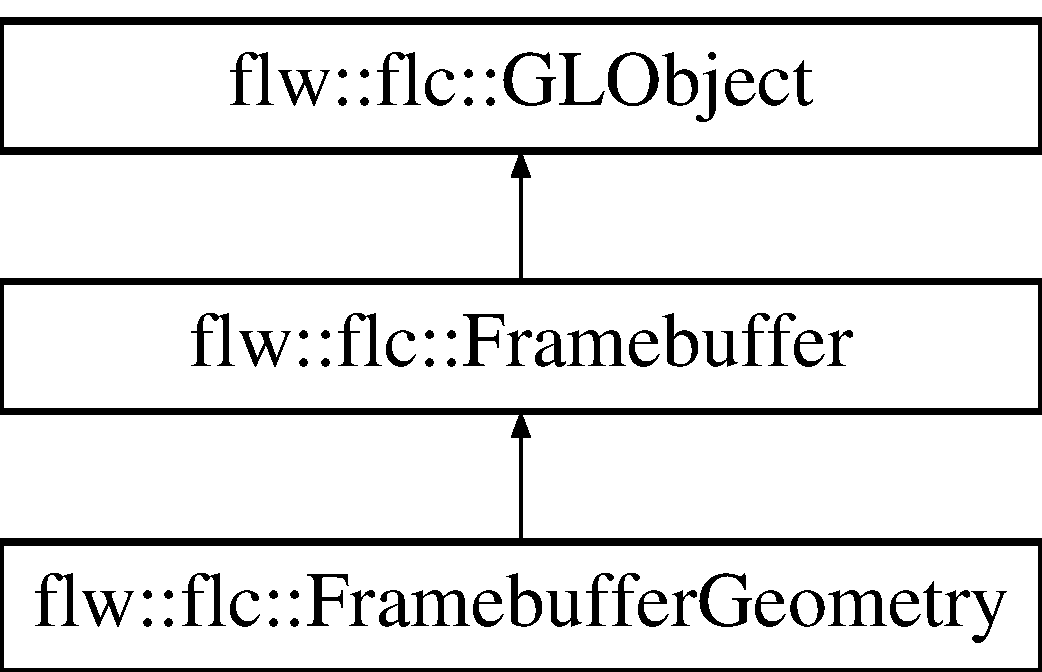
\includegraphics[height=3.000000cm]{classflw_1_1flc_1_1FramebufferGeometry}
\end{center}
\end{figure}
\subsection*{Public Member Functions}
\begin{DoxyCompactItemize}
\item 
{\bfseries Framebuffer\+Geometry} (\hyperlink{classflw_1_1flf_1_1TextureSystem}{flf\+::\+Texture\+System} \&textures, G\+Luint width, G\+Luint height, G\+Luint color\+Buffers, G\+Luint depth\+Buffers)\hypertarget{classflw_1_1flc_1_1FramebufferGeometry_a73ef82a08dabc4ab9f22532739280a3a}{}\label{classflw_1_1flc_1_1FramebufferGeometry_a73ef82a08dabc4ab9f22532739280a3a}

\item 
void {\bfseries bind\+Attachments} ()\hypertarget{classflw_1_1flc_1_1FramebufferGeometry_af50fc97cbd0dcaa71b0d1e394df904ff}{}\label{classflw_1_1flc_1_1FramebufferGeometry_af50fc97cbd0dcaa71b0d1e394df904ff}

\item 
void {\bfseries set\+Attachments} ()\hypertarget{classflw_1_1flc_1_1FramebufferGeometry_a2a6d3c1726f0ad74753754ff4ea93ee4}{}\label{classflw_1_1flc_1_1FramebufferGeometry_a2a6d3c1726f0ad74753754ff4ea93ee4}

\item 
void {\bfseries set\+Attachment\+Stencil\+Depth} ()\hypertarget{classflw_1_1flc_1_1FramebufferGeometry_a4bf62a57889b708f77eca52019d2d329}{}\label{classflw_1_1flc_1_1FramebufferGeometry_a4bf62a57889b708f77eca52019d2d329}

\item 
void {\bfseries set\+Attachment\+Summary\+For\+Reading} ()\hypertarget{classflw_1_1flc_1_1FramebufferGeometry_a6eb7626820ef3a809e2b991623a94371}{}\label{classflw_1_1flc_1_1FramebufferGeometry_a6eb7626820ef3a809e2b991623a94371}

\item 
void {\bfseries set\+Attachment\+Summary\+For\+Writing} ()\hypertarget{classflw_1_1flc_1_1FramebufferGeometry_a87cd7514a43b439abf9600898e586cfe}{}\label{classflw_1_1flc_1_1FramebufferGeometry_a87cd7514a43b439abf9600898e586cfe}

\item 
void {\bfseries resize} (G\+Luint width, G\+Luint height)\hypertarget{classflw_1_1flc_1_1FramebufferGeometry_a63dd366139773a4fd028a9b8fb98f150}{}\label{classflw_1_1flc_1_1FramebufferGeometry_a63dd366139773a4fd028a9b8fb98f150}

\item 
void {\bfseries reload} ()\hypertarget{classflw_1_1flc_1_1FramebufferGeometry_a7e1c50e4964c2d595ad344086239189d}{}\label{classflw_1_1flc_1_1FramebufferGeometry_a7e1c50e4964c2d595ad344086239189d}

\end{DoxyCompactItemize}
\subsection*{Additional Inherited Members}


\subsection{Detailed Description}
\hyperlink{classflw_1_1flc_1_1Framebuffer}{Framebuffer} with multiple color and depth attachments. 

The documentation for this class was generated from the following file\+:\begin{DoxyCompactItemize}
\item 
/home/filip/\+Projects/fillwave/inc/fillwave/core/rendering/Framebuffer\+Geometry.\+h\end{DoxyCompactItemize}

\hypertarget{classflw_1_1flc_1_1GLObject}{}\section{flw\+:\+:flc\+:\+:G\+L\+Object Class Reference}
\label{classflw_1_1flc_1_1GLObject}\index{flw\+::flc\+::\+G\+L\+Object@{flw\+::flc\+::\+G\+L\+Object}}


Base class for all Open\+GL objects not related to pipeline.  




{\ttfamily \#include $<$G\+L\+Object.\+h$>$}

Inheritance diagram for flw\+:\+:flc\+:\+:G\+L\+Object\+:\begin{figure}[H]
\begin{center}
\leavevmode
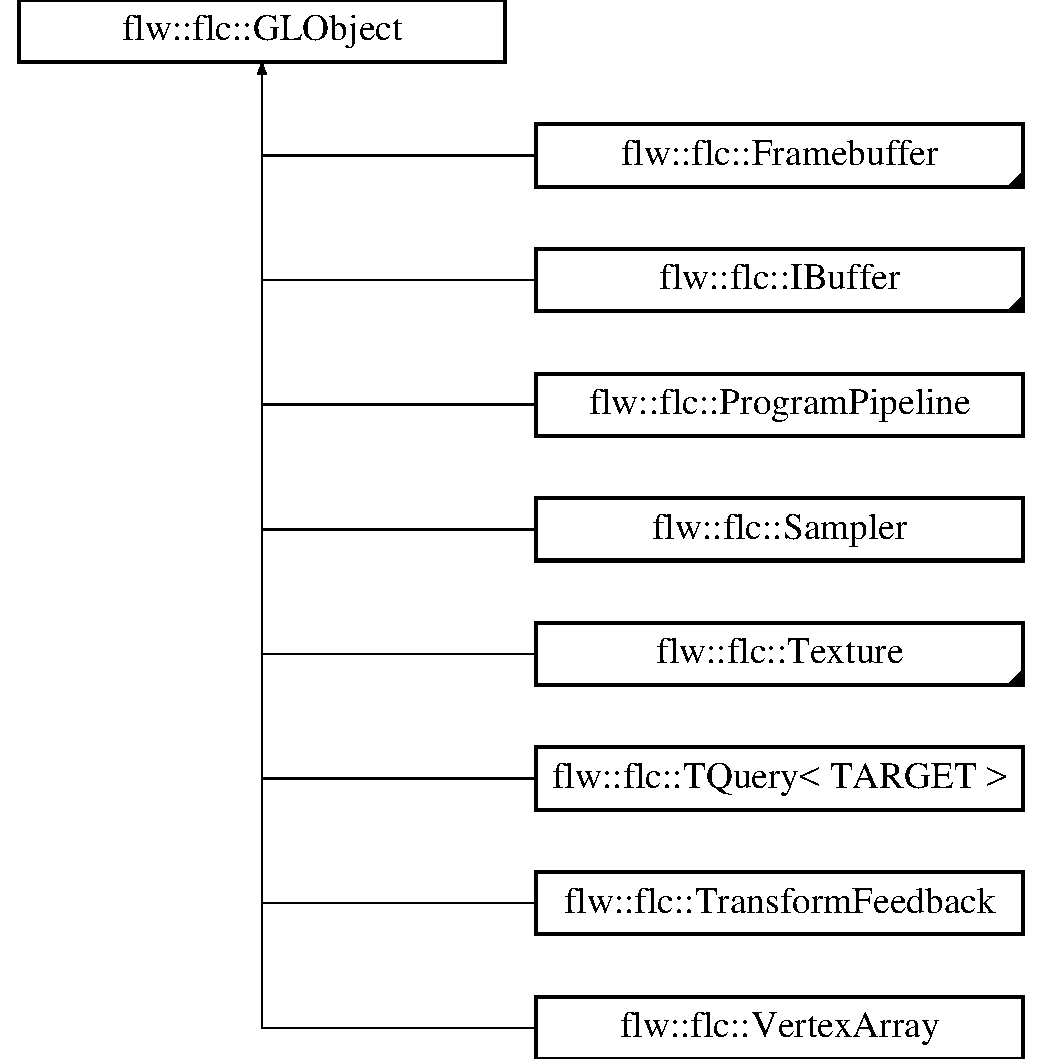
\includegraphics[height=9.000000cm]{classflw_1_1flc_1_1GLObject}
\end{center}
\end{figure}
\subsection*{Public Member Functions}
\begin{DoxyCompactItemize}
\item 
\mbox{\Hypertarget{classflw_1_1flc_1_1GLObject_aec8d37982901c84d58f9319c863d0e24}\label{classflw_1_1flc_1_1GLObject_aec8d37982901c84d58f9319c863d0e24}} 
{\bfseries G\+L\+Object} (G\+Lsizei how\+Many)
\item 
\mbox{\Hypertarget{classflw_1_1flc_1_1GLObject_ac23c3ec039eccfbed64799352df3dbce}\label{classflw_1_1flc_1_1GLObject_ac23c3ec039eccfbed64799352df3dbce}} 
G\+Luint {\bfseries get\+Handle} (G\+Luint id=0)
\end{DoxyCompactItemize}
\subsection*{Protected Attributes}
\begin{DoxyCompactItemize}
\item 
\mbox{\Hypertarget{classflw_1_1flc_1_1GLObject_a295b5e3514f7b8f16cd0f9e73f3071f3}\label{classflw_1_1flc_1_1GLObject_a295b5e3514f7b8f16cd0f9e73f3071f3}} 
G\+Lsizei {\bfseries m\+How\+Many}
\item 
\mbox{\Hypertarget{classflw_1_1flc_1_1GLObject_a7a46e87fca26ddc35dc2ccb930b454f3}\label{classflw_1_1flc_1_1GLObject_a7a46e87fca26ddc35dc2ccb930b454f3}} 
G\+Luint {\bfseries m\+Handles} \mbox{[}M\+A\+X\+\_\+\+E\+L\+E\+M\+E\+N\+TS\mbox{]}
\end{DoxyCompactItemize}


\subsection{Detailed Description}
Base class for all Open\+GL objects not related to pipeline. 

The documentation for this class was generated from the following file\+:\begin{DoxyCompactItemize}
\item 
/home/filip/projects/fillwave/inc/fillwave/core/G\+L\+Object.\+h\end{DoxyCompactItemize}

\hypertarget{classflw_1_1flf_1_1Hinge}{}\section{flw\+:\+:flf\+:\+:Hinge Class Reference}
\label{classflw_1_1flf_1_1Hinge}\index{flw\+::flf\+::\+Hinge@{flw\+::flf\+::\+Hinge}}


\hyperlink{classflw_1_1flf_1_1Entity}{Entity} capable of populating the draw method towards children.  




{\ttfamily \#include $<$Hinge.\+h$>$}

Inheritance diagram for flw\+:\+:flf\+:\+:Hinge\+:\begin{figure}[H]
\begin{center}
\leavevmode
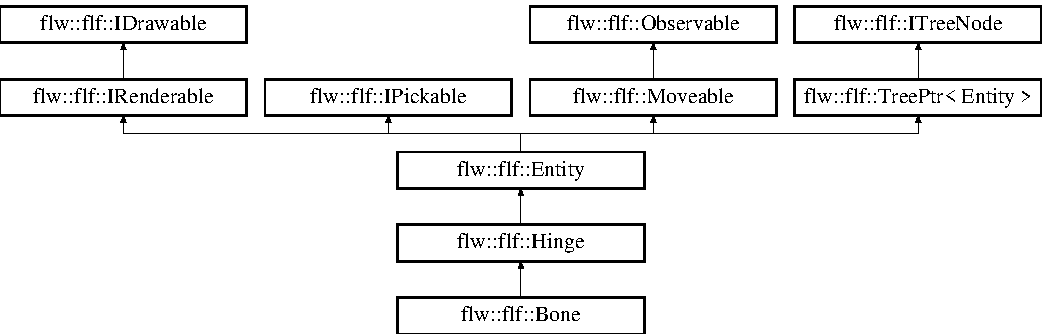
\includegraphics[height=4.487180cm]{classflw_1_1flf_1_1Hinge}
\end{center}
\end{figure}
\subsection*{Public Member Functions}
\begin{DoxyCompactItemize}
\item 
\mbox{\Hypertarget{classflw_1_1flf_1_1Hinge_a7eaaa5d2d2a1e2f3c6c6500031d0cab6}\label{classflw_1_1flf_1_1Hinge_a7eaaa5d2d2a1e2f3c6c6500031d0cab6}} 
void {\bfseries draw} (\hyperlink{classflw_1_1flf_1_1ICamera}{I\+Camera} \&camera) override
\item 
\mbox{\Hypertarget{classflw_1_1flf_1_1Hinge_ac9aed70e3fbed2d4e2bb40b1248f2955}\label{classflw_1_1flf_1_1Hinge_ac9aed70e3fbed2d4e2bb40b1248f2955}} 
void {\bfseries draw\+P\+B\+RP} (\hyperlink{classflw_1_1flf_1_1ICamera}{I\+Camera} \&camera) override
\item 
\mbox{\Hypertarget{classflw_1_1flf_1_1Hinge_a4e7c9e2e2cd5a3f9a5fbd1d9b24c13c0}\label{classflw_1_1flf_1_1Hinge_a4e7c9e2e2cd5a3f9a5fbd1d9b24c13c0}} 
void {\bfseries draw\+DR} (\hyperlink{classflw_1_1flf_1_1ICamera}{I\+Camera} \&camera) override
\item 
\mbox{\Hypertarget{classflw_1_1flf_1_1Hinge_a6c71b26eba2726415d89f281de5be6d1}\label{classflw_1_1flf_1_1Hinge_a6c71b26eba2726415d89f281de5be6d1}} 
void {\bfseries update\+Renderer} (\hyperlink{classflw_1_1flf_1_1IRenderer}{I\+Renderer} \&renderer) override
\item 
\mbox{\Hypertarget{classflw_1_1flf_1_1Hinge_a6cc851b6a7ce956c6a16ec4fe1f30585}\label{classflw_1_1flf_1_1Hinge_a6cc851b6a7ce956c6a16ec4fe1f30585}} 
bool {\bfseries get\+Render\+Item} (\hyperlink{structflw_1_1flf_1_1RenderItem}{Render\+Item} \&item) override
\end{DoxyCompactItemize}
\subsection*{Additional Inherited Members}


\subsection{Detailed Description}
\hyperlink{classflw_1_1flf_1_1Entity}{Entity} capable of populating the draw method towards children. 

The documentation for this class was generated from the following file\+:\begin{DoxyCompactItemize}
\item 
/home/filip/projects/fillwave/inc/fillwave/models/animations/Hinge.\+h\end{DoxyCompactItemize}

\hypertarget{classflw_1_1flf_1_1HUD}{}\section{flw\+:\+:flf\+:\+:H\+UD Class Reference}
\label{classflw_1_1flf_1_1HUD}\index{flw\+::flf\+::\+H\+UD@{flw\+::flf\+::\+H\+UD}}


Heads Up Display tree.  




{\ttfamily \#include $<$H\+U\+D.\+h$>$}

Inheritance diagram for flw\+:\+:flf\+:\+:H\+UD\+:\begin{figure}[H]
\begin{center}
\leavevmode
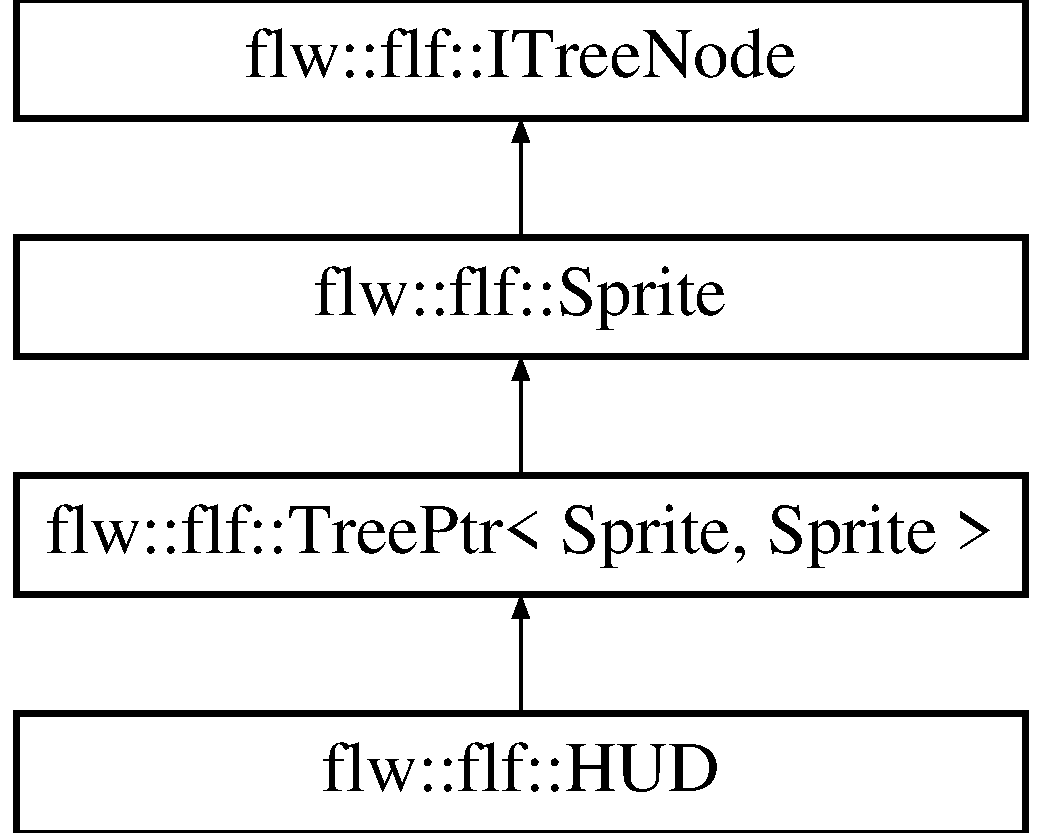
\includegraphics[height=4.000000cm]{classflw_1_1flf_1_1HUD}
\end{center}
\end{figure}
\subsection*{Public Member Functions}
\begin{DoxyCompactItemize}
\item 
\mbox{\Hypertarget{classflw_1_1flf_1_1HUD_a3392d188f610fe9eba0c701236da0569}\label{classflw_1_1flf_1_1HUD_a3392d188f610fe9eba0c701236da0569}} 
virtual void {\bfseries draw} () override
\end{DoxyCompactItemize}
\subsection*{Additional Inherited Members}


\subsection{Detailed Description}
Heads Up Display tree. 

The documentation for this class was generated from the following file\+:\begin{DoxyCompactItemize}
\item 
/home/filip/projects/fillwave/inc/fillwave/hud/base/H\+U\+D.\+h\end{DoxyCompactItemize}

\hypertarget{classflw_1_1flc_1_1IBuffer}{}\section{flw\+:\+:flc\+:\+:I\+Buffer Class Reference}
\label{classflw_1_1flc_1_1IBuffer}\index{flw\+::flc\+::\+I\+Buffer@{flw\+::flc\+::\+I\+Buffer}}


Base for all buffer types.  




{\ttfamily \#include $<$I\+Buffer.\+h$>$}

Inheritance diagram for flw\+:\+:flc\+:\+:I\+Buffer\+:\begin{figure}[H]
\begin{center}
\leavevmode
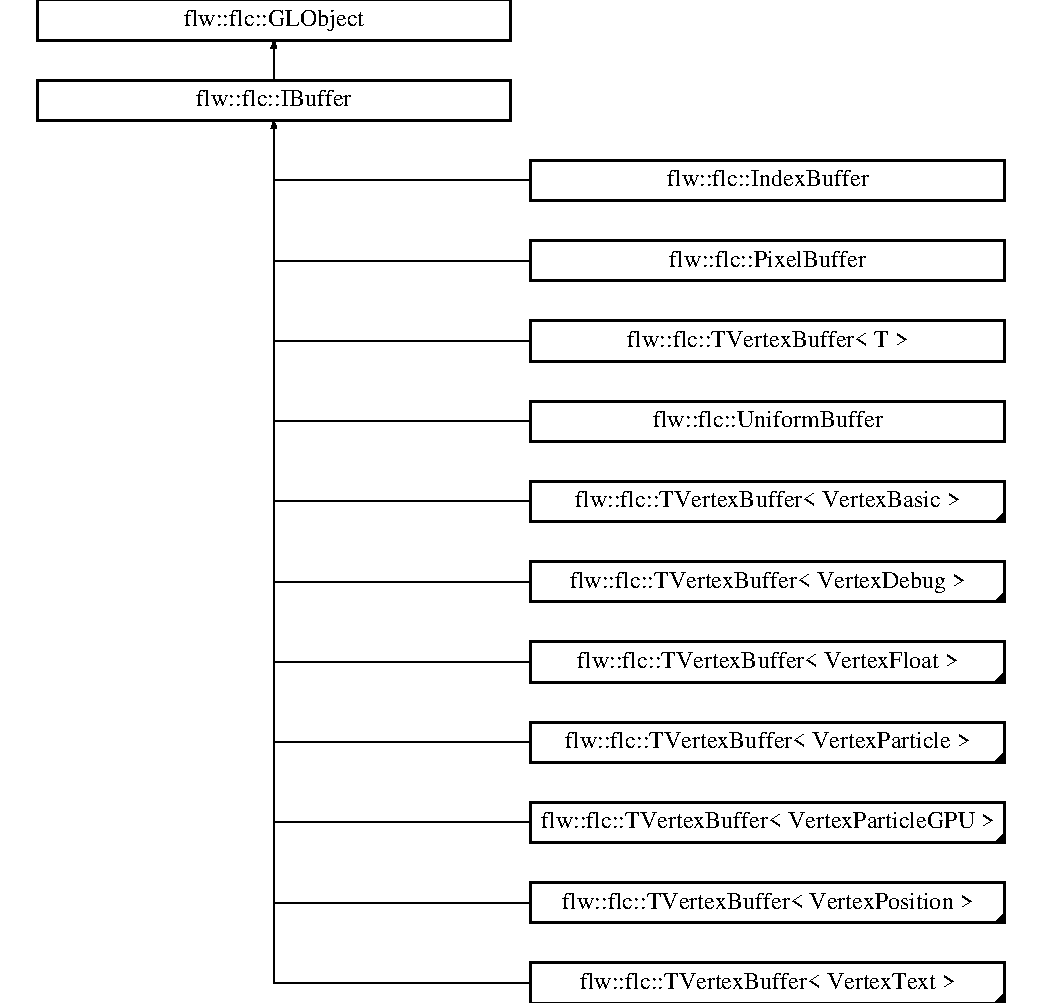
\includegraphics[height=12.000000cm]{classflw_1_1flc_1_1IBuffer}
\end{center}
\end{figure}
\subsection*{Public Member Functions}
\begin{DoxyCompactItemize}
\item 
{\bfseries I\+Buffer} (G\+Luint target, G\+Luint draw\+Type=G\+L\+\_\+\+S\+T\+A\+T\+I\+C\+\_\+\+D\+R\+AW, G\+Luint index=0, G\+Lsizei how\+Many=1)\hypertarget{classflw_1_1flc_1_1IBuffer_ad7053cc22011388104c4bcc6ca05599e}{}\label{classflw_1_1flc_1_1IBuffer_ad7053cc22011388104c4bcc6ca05599e}

\item 
void {\bfseries bind} (G\+Luint id=0) const \hypertarget{classflw_1_1flc_1_1IBuffer_ac45d3729b5e4b1fe52d79275a94c4ccc}{}\label{classflw_1_1flc_1_1IBuffer_ac45d3729b5e4b1fe52d79275a94c4ccc}

\item 
void {\bfseries bind} (G\+Luint external\+Target, G\+Luint id) const \hypertarget{classflw_1_1flc_1_1IBuffer_a4d02d0364f840398c213f6c7f9700d8e}{}\label{classflw_1_1flc_1_1IBuffer_a4d02d0364f840398c213f6c7f9700d8e}

\item 
void {\bfseries bind\+Base} (G\+Luint id=0) const \hypertarget{classflw_1_1flc_1_1IBuffer_af229d6fa4fbb30bacb81dcac734db783}{}\label{classflw_1_1flc_1_1IBuffer_af229d6fa4fbb30bacb81dcac734db783}

\item 
void {\bfseries bind\+Base} (G\+Luint external\+Target, G\+Luint id) const \hypertarget{classflw_1_1flc_1_1IBuffer_ab64c3e009a119394f895b3dacf4cc665}{}\label{classflw_1_1flc_1_1IBuffer_ab64c3e009a119394f895b3dacf4cc665}

\item 
void {\bfseries unbind} ()\hypertarget{classflw_1_1flc_1_1IBuffer_aa838099c22a2799d4cad641f8d40e674}{}\label{classflw_1_1flc_1_1IBuffer_aa838099c22a2799d4cad641f8d40e674}

\item 
void {\bfseries unbind\+Base} (G\+Luint external\+Target)\hypertarget{classflw_1_1flc_1_1IBuffer_a1321b63bca1153b09b914f9ca8d52b2a}{}\label{classflw_1_1flc_1_1IBuffer_a1321b63bca1153b09b914f9ca8d52b2a}

\item 
void {\bfseries unmap} () const \hypertarget{classflw_1_1flc_1_1IBuffer_adb045f3a301425168ba2b2bd9009c876}{}\label{classflw_1_1flc_1_1IBuffer_adb045f3a301425168ba2b2bd9009c876}

\item 
void {\bfseries send} ()\hypertarget{classflw_1_1flc_1_1IBuffer_a0fa4b45e543ed7f945f8d216628e7c53}{}\label{classflw_1_1flc_1_1IBuffer_a0fa4b45e543ed7f945f8d216628e7c53}

\item 
void {\bfseries set\+Target} (G\+Luint target)\hypertarget{classflw_1_1flc_1_1IBuffer_a7d73a5dcb2cc252fe329565a4c329433}{}\label{classflw_1_1flc_1_1IBuffer_a7d73a5dcb2cc252fe329565a4c329433}

\item 
void {\bfseries set\+Draw\+Type} (G\+Luint draw\+Type)\hypertarget{classflw_1_1flc_1_1IBuffer_a641903dd05dbe080d8f761ec55bffa97}{}\label{classflw_1_1flc_1_1IBuffer_a641903dd05dbe080d8f761ec55bffa97}

\item 
bool {\bfseries is\+Loaded} ()\hypertarget{classflw_1_1flc_1_1IBuffer_a5d6c3aea1c1ea096aa9f27197bb0cd64}{}\label{classflw_1_1flc_1_1IBuffer_a5d6c3aea1c1ea096aa9f27197bb0cd64}

\item 
void {\bfseries set\+Loaded} (bool loaded)\hypertarget{classflw_1_1flc_1_1IBuffer_a27fe03746857f00fb4631c73645a3a3a}{}\label{classflw_1_1flc_1_1IBuffer_a27fe03746857f00fb4631c73645a3a3a}

\item 
G\+Luint {\bfseries get\+Elements} () const \hypertarget{classflw_1_1flc_1_1IBuffer_aa7dc7de3135438e773925f58034125de}{}\label{classflw_1_1flc_1_1IBuffer_aa7dc7de3135438e773925f58034125de}

\item 
G\+Luint {\bfseries get\+Size} () const \hypertarget{classflw_1_1flc_1_1IBuffer_aa2ae6b3c9491fa3f5c3ca4d45b738215}{}\label{classflw_1_1flc_1_1IBuffer_aa2ae6b3c9491fa3f5c3ca4d45b738215}

\item 
G\+Lvoid $\ast$ {\bfseries get\+Data} () const \hypertarget{classflw_1_1flc_1_1IBuffer_a3962d189ef43bc43d247c5bff7ccc5e1}{}\label{classflw_1_1flc_1_1IBuffer_a3962d189ef43bc43d247c5bff7ccc5e1}

\item 
void {\bfseries reload} ()\hypertarget{classflw_1_1flc_1_1IBuffer_a3336186b4cabbfd41764d594856ea470}{}\label{classflw_1_1flc_1_1IBuffer_a3336186b4cabbfd41764d594856ea470}

\item 
G\+Lvoid $\ast$ {\bfseries map\+Range} (G\+Lenum access, G\+Luint size=0)\hypertarget{classflw_1_1flc_1_1IBuffer_a1a24ce0fc4b8c5bfcc684deb7173c493}{}\label{classflw_1_1flc_1_1IBuffer_a1a24ce0fc4b8c5bfcc684deb7173c493}

\item 
G\+Lvoid $\ast$ {\bfseries map} (G\+Lenum access) const \hypertarget{classflw_1_1flc_1_1IBuffer_ab8174b93310fb75d673246a6c0e84901}{}\label{classflw_1_1flc_1_1IBuffer_ab8174b93310fb75d673246a6c0e84901}

\item 
virtual void {\bfseries empty\+C\+PU} ()=0\hypertarget{classflw_1_1flc_1_1IBuffer_a947b4716bdab96de09bf448211189ad7}{}\label{classflw_1_1flc_1_1IBuffer_a947b4716bdab96de09bf448211189ad7}

\item 
virtual void {\bfseries empty\+G\+PU} ()=0\hypertarget{classflw_1_1flc_1_1IBuffer_ac3793d00dbfcc62b7b78cd9c6edac746}{}\label{classflw_1_1flc_1_1IBuffer_ac3793d00dbfcc62b7b78cd9c6edac746}

\end{DoxyCompactItemize}
\subsection*{Protected Member Functions}
\begin{DoxyCompactItemize}
\item 
void {\bfseries set\+Elements} (G\+Luint elements)\hypertarget{classflw_1_1flc_1_1IBuffer_abfef8a1d484a0a974e1b68899b94793e}{}\label{classflw_1_1flc_1_1IBuffer_abfef8a1d484a0a974e1b68899b94793e}

\item 
void {\bfseries set\+Size} (G\+Luint size)\hypertarget{classflw_1_1flc_1_1IBuffer_a07a92c12bc564ea26ef2091915b992e3}{}\label{classflw_1_1flc_1_1IBuffer_a07a92c12bc564ea26ef2091915b992e3}

\end{DoxyCompactItemize}
\subsection*{Protected Attributes}
\begin{DoxyCompactItemize}
\item 
bool {\bfseries m\+Loaded}\hypertarget{classflw_1_1flc_1_1IBuffer_a7012500f1c886ae84e9bd7d878f70a8b}{}\label{classflw_1_1flc_1_1IBuffer_a7012500f1c886ae84e9bd7d878f70a8b}

\item 
G\+Luint {\bfseries m\+Target}\hypertarget{classflw_1_1flc_1_1IBuffer_a3d34efd1977e2ea9b859b32458c23236}{}\label{classflw_1_1flc_1_1IBuffer_a3d34efd1977e2ea9b859b32458c23236}

\item 
G\+Luint {\bfseries m\+Data\+Store\+Type}\hypertarget{classflw_1_1flc_1_1IBuffer_a099516254495f4a99e65121816d02bab}{}\label{classflw_1_1flc_1_1IBuffer_a099516254495f4a99e65121816d02bab}

\item 
G\+Luint {\bfseries m\+Index}\hypertarget{classflw_1_1flc_1_1IBuffer_ad6cf73186e60ec40248b14c5b11f00ee}{}\label{classflw_1_1flc_1_1IBuffer_ad6cf73186e60ec40248b14c5b11f00ee}

\item 
G\+Lvoid $\ast$ {\bfseries m\+Data}\hypertarget{classflw_1_1flc_1_1IBuffer_ad576bb156f18bf6050414445ce768737}{}\label{classflw_1_1flc_1_1IBuffer_ad576bb156f18bf6050414445ce768737}

\item 
G\+Lulong {\bfseries m\+Size}\hypertarget{classflw_1_1flc_1_1IBuffer_af6d84c87b8a85e193de1c7d62e0c5098}{}\label{classflw_1_1flc_1_1IBuffer_af6d84c87b8a85e193de1c7d62e0c5098}

\item 
G\+Lulong {\bfseries m\+Total\+Elements}\hypertarget{classflw_1_1flc_1_1IBuffer_a64fbd477df8e2731e70198cf43f59577}{}\label{classflw_1_1flc_1_1IBuffer_a64fbd477df8e2731e70198cf43f59577}

\end{DoxyCompactItemize}


\subsection{Detailed Description}
Base for all buffer types. 

The documentation for this class was generated from the following file\+:\begin{DoxyCompactItemize}
\item 
/home/filip/\+Projects/fillwave/inc/fillwave/core/buffers/I\+Buffer.\+h\end{DoxyCompactItemize}

\hypertarget{classflw_1_1flf_1_1ICamera}{}\section{flw\+:\+:flf\+:\+:I\+Camera Class Reference}
\label{classflw_1_1flf_1_1ICamera}\index{flw\+::flf\+::\+I\+Camera@{flw\+::flf\+::\+I\+Camera}}


Stores camera view parameters.  




{\ttfamily \#include $<$I\+Camera.\+h$>$}

Inheritance diagram for flw\+:\+:flf\+:\+:I\+Camera\+:\begin{figure}[H]
\begin{center}
\leavevmode
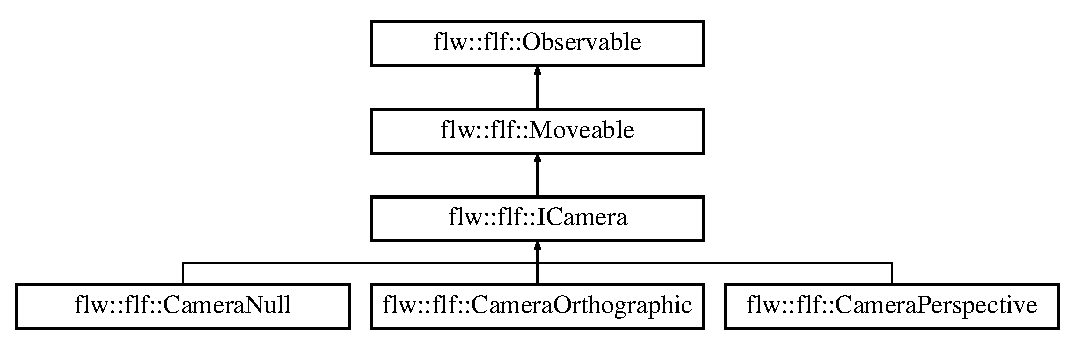
\includegraphics[height=4.000000cm]{classflw_1_1flf_1_1ICamera}
\end{center}
\end{figure}
\subsection*{Public Member Functions}
\begin{DoxyCompactItemize}
\item 
\mbox{\Hypertarget{classflw_1_1flf_1_1ICamera_a3a28d3603bc703fc2abf412f30e17cde}\label{classflw_1_1flf_1_1ICamera_a3a28d3603bc703fc2abf412f30e17cde}} 
{\bfseries I\+Camera} (glm\+::vec3, glm\+::quat rotation)
\item 
\mbox{\Hypertarget{classflw_1_1flf_1_1ICamera_a9fcc6a75bb0f49d7308396eec9105a89}\label{classflw_1_1flf_1_1ICamera_a9fcc6a75bb0f49d7308396eec9105a89}} 
void {\bfseries update} ()
\item 
\mbox{\Hypertarget{classflw_1_1flf_1_1ICamera_a364eb58aa13b0ac004cdfd0c270d9b5a}\label{classflw_1_1flf_1_1ICamera_a364eb58aa13b0ac004cdfd0c270d9b5a}} 
void {\bfseries update\+View} ()
\item 
\mbox{\Hypertarget{classflw_1_1flf_1_1ICamera_a13edf1c6809a1d64fda00ac05c3e26b6}\label{classflw_1_1flf_1_1ICamera_a13edf1c6809a1d64fda00ac05c3e26b6}} 
glm\+::mat4 {\bfseries get\+Eye} ()
\item 
\mbox{\Hypertarget{classflw_1_1flf_1_1ICamera_a2dd407fba655d57f74f2cba0de9ec978}\label{classflw_1_1flf_1_1ICamera_a2dd407fba655d57f74f2cba0de9ec978}} 
glm\+::mat4 {\bfseries get\+Projection} ()
\item 
\mbox{\Hypertarget{classflw_1_1flf_1_1ICamera_a8af0d020d8a6a10a68f65162806c8a98}\label{classflw_1_1flf_1_1ICamera_a8af0d020d8a6a10a68f65162806c8a98}} 
glm\+::mat4 {\bfseries get\+View\+Projection} ()
\item 
\mbox{\Hypertarget{classflw_1_1flf_1_1ICamera_a16c68d1fa6e5f7159a14c6aa018d1a84}\label{classflw_1_1flf_1_1ICamera_a16c68d1fa6e5f7159a14c6aa018d1a84}} 
virtual void {\bfseries update\+Projection} ()=0
\item 
\mbox{\Hypertarget{classflw_1_1flf_1_1ICamera_aa6edd27ce33e246e70b946c1267406d6}\label{classflw_1_1flf_1_1ICamera_aa6edd27ce33e246e70b946c1267406d6}} 
virtual G\+Lfloat {\bfseries get\+Projection\+Near\+Plane} ()=0
\item 
\mbox{\Hypertarget{classflw_1_1flf_1_1ICamera_a702a10b338e2612e673538d7f61ef289}\label{classflw_1_1flf_1_1ICamera_a702a10b338e2612e673538d7f61ef289}} 
virtual G\+Lfloat {\bfseries get\+Projection\+Far\+Plane} ()=0
\item 
\mbox{\Hypertarget{classflw_1_1flf_1_1ICamera_ae7d388dbed85e70473f3d0b59798d3b4}\label{classflw_1_1flf_1_1ICamera_ae7d388dbed85e70473f3d0b59798d3b4}} 
virtual void {\bfseries log} () const
\end{DoxyCompactItemize}
\subsection*{Protected Attributes}
\begin{DoxyCompactItemize}
\item 
\mbox{\Hypertarget{classflw_1_1flf_1_1ICamera_a96135bcf2aa431c21ff72586e6857cde}\label{classflw_1_1flf_1_1ICamera_a96135bcf2aa431c21ff72586e6857cde}} 
glm\+::mat4 {\bfseries m\+Camera\+Matrix}
\item 
\mbox{\Hypertarget{classflw_1_1flf_1_1ICamera_aa42f67c78d9102d1a0145c5d115e962a}\label{classflw_1_1flf_1_1ICamera_aa42f67c78d9102d1a0145c5d115e962a}} 
glm\+::mat4 {\bfseries m\+Projection\+Matrix}
\item 
\mbox{\Hypertarget{classflw_1_1flf_1_1ICamera_a53df3590abc5d8e52fc7d88cf42a3c61}\label{classflw_1_1flf_1_1ICamera_a53df3590abc5d8e52fc7d88cf42a3c61}} 
G\+Lboolean {\bfseries m\+Refresh\+View}
\item 
\mbox{\Hypertarget{classflw_1_1flf_1_1ICamera_a6553d3e78499407b28e40a149a4fc3e8}\label{classflw_1_1flf_1_1ICamera_a6553d3e78499407b28e40a149a4fc3e8}} 
G\+Lboolean {\bfseries m\+Refresh\+Projection}
\end{DoxyCompactItemize}


\subsection{Detailed Description}
Stores camera view parameters. 

The documentation for this class was generated from the following file\+:\begin{DoxyCompactItemize}
\item 
/home/filip/projects/fillwave/inc/fillwave/space/base/I\+Camera.\+h\end{DoxyCompactItemize}

\hypertarget{classflw_1_1flf_1_1IDrawable}{}\section{flw\+:\+:flf\+:\+:I\+Drawable Class Reference}
\label{classflw_1_1flf_1_1IDrawable}\index{flw\+::flf\+::\+I\+Drawable@{flw\+::flf\+::\+I\+Drawable}}


Drawing interface.  




{\ttfamily \#include $<$I\+Drawable.\+h$>$}

Inheritance diagram for flw\+:\+:flf\+:\+:I\+Drawable\+:\begin{figure}[H]
\begin{center}
\leavevmode
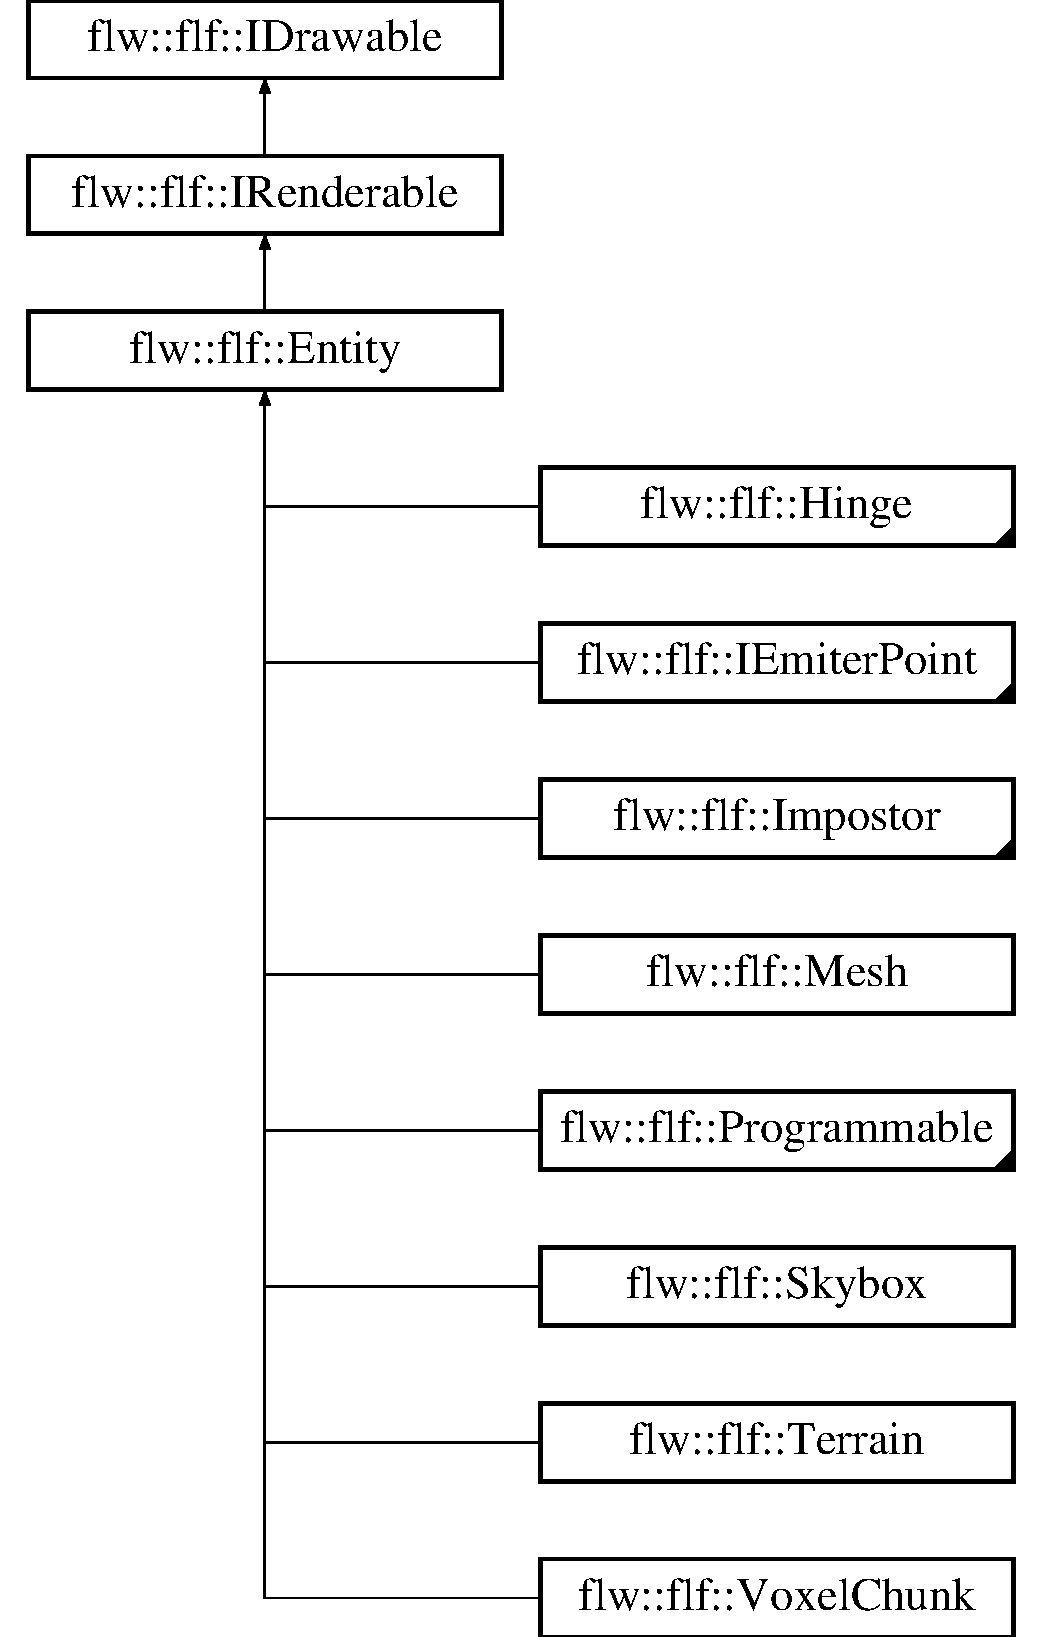
\includegraphics[height=11.000000cm]{classflw_1_1flf_1_1IDrawable}
\end{center}
\end{figure}
\subsection*{Public Member Functions}
\begin{DoxyCompactItemize}
\item 
\mbox{\Hypertarget{classflw_1_1flf_1_1IDrawable_ad94201dc7ac4f3e94b86b0b8d8d6b597}\label{classflw_1_1flf_1_1IDrawable_ad94201dc7ac4f3e94b86b0b8d8d6b597}} 
virtual void {\bfseries draw} (\hyperlink{classflw_1_1flf_1_1ICamera}{I\+Camera} \&camera)=0
\item 
\mbox{\Hypertarget{classflw_1_1flf_1_1IDrawable_aaadbf5d74624af32ea8b5064502aced0}\label{classflw_1_1flf_1_1IDrawable_aaadbf5d74624af32ea8b5064502aced0}} 
virtual void {\bfseries draw\+P\+B\+RP} (\hyperlink{classflw_1_1flf_1_1ICamera}{I\+Camera} \&camera)=0
\item 
\mbox{\Hypertarget{classflw_1_1flf_1_1IDrawable_a38b6d894083451f43f220d96f73a8a65}\label{classflw_1_1flf_1_1IDrawable_a38b6d894083451f43f220d96f73a8a65}} 
virtual void {\bfseries draw\+DR} (\hyperlink{classflw_1_1flf_1_1ICamera}{I\+Camera} \&camera)=0
\item 
\mbox{\Hypertarget{classflw_1_1flf_1_1IDrawable_a38142c33f088087a0c2c7879a73d9c72}\label{classflw_1_1flf_1_1IDrawable_a38142c33f088087a0c2c7879a73d9c72}} 
virtual void {\bfseries draw\+Depth} (\hyperlink{classflw_1_1flf_1_1ICamera}{I\+Camera} \&camera)=0
\item 
\mbox{\Hypertarget{classflw_1_1flf_1_1IDrawable_ae67b0f617e1e0cc5fb4fb63d7df95a41}\label{classflw_1_1flf_1_1IDrawable_ae67b0f617e1e0cc5fb4fb63d7df95a41}} 
virtual void {\bfseries draw\+Depth\+Color} (\hyperlink{classflw_1_1flf_1_1ICamera}{I\+Camera} \&camera, glm\+::vec3 \&position)=0
\item 
\mbox{\Hypertarget{classflw_1_1flf_1_1IDrawable_a3b98b73690d52c7638dad261e7180914}\label{classflw_1_1flf_1_1IDrawable_a3b98b73690d52c7638dad261e7180914}} 
virtual void {\bfseries draw\+A\+OG} (\hyperlink{classflw_1_1flf_1_1ICamera}{I\+Camera} \&camera)=0
\item 
\mbox{\Hypertarget{classflw_1_1flf_1_1IDrawable_af5096dd51585f38717f0d250cc839ad0}\label{classflw_1_1flf_1_1IDrawable_af5096dd51585f38717f0d250cc839ad0}} 
virtual void {\bfseries draw\+A\+OC} (\hyperlink{classflw_1_1flf_1_1ICamera}{I\+Camera} \&camera)=0
\item 
\mbox{\Hypertarget{classflw_1_1flf_1_1IDrawable_a479fa858127eb85c200ad32bd672c3e9}\label{classflw_1_1flf_1_1IDrawable_a479fa858127eb85c200ad32bd672c3e9}} 
virtual void {\bfseries draw\+Occlusion\+Box} (\hyperlink{classflw_1_1flf_1_1ICamera}{I\+Camera} \&camera)=0
\item 
\mbox{\Hypertarget{classflw_1_1flf_1_1IDrawable_a497b4bf675dca36654e98f114cd6953f}\label{classflw_1_1flf_1_1IDrawable_a497b4bf675dca36654e98f114cd6953f}} 
virtual void {\bfseries draw\+Picking} (\hyperlink{classflw_1_1flf_1_1ICamera}{I\+Camera} \&camera)=0
\end{DoxyCompactItemize}


\subsection{Detailed Description}
Drawing interface. 

The documentation for this class was generated from the following file\+:\begin{DoxyCompactItemize}
\item 
/home/filip/projects/fillwave/inc/fillwave/models/base/I\+Drawable.\+h\end{DoxyCompactItemize}

\hypertarget{classflw_1_1flf_1_1IEffect}{}\section{flw\+:\+:flf\+:\+:I\+Effect Class Reference}
\label{classflw_1_1flf_1_1IEffect}\index{flw\+::flf\+::\+I\+Effect@{flw\+::flf\+::\+I\+Effect}}


Base for effects.  




{\ttfamily \#include $<$Effect.\+h$>$}

Inheritance diagram for flw\+:\+:flf\+:\+:I\+Effect\+:\begin{figure}[H]
\begin{center}
\leavevmode
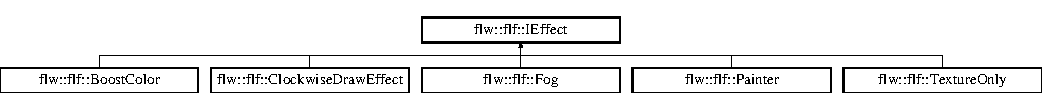
\includegraphics[height=1.251397cm]{classflw_1_1flf_1_1IEffect}
\end{center}
\end{figure}
\subsection*{Public Member Functions}
\begin{DoxyCompactItemize}
\item 
virtual void \hyperlink{classflw_1_1flf_1_1IEffect_ae65eed21e40a226c7739d3c5dedd9e50}{pre\+Draw\+Action} (\hyperlink{classflw_1_1flc_1_1Program}{flc\+::\+Program} $\ast$program)=0
\begin{DoxyCompactList}\small\item\em virtual\+: defines action to be done just before the draw. \end{DoxyCompactList}\item 
virtual void \hyperlink{classflw_1_1flf_1_1IEffect_a6bb11d90e7e4da057ca398bd8c61208a}{post\+Draw\+Action} (\hyperlink{classflw_1_1flc_1_1Program}{flc\+::\+Program} $\ast$program)=0
\begin{DoxyCompactList}\small\item\em virtual\+: defines action to be done just after the draw. \end{DoxyCompactList}\item 
virtual void \hyperlink{classflw_1_1flf_1_1IEffect_a1a03eaf63a9d4edbd8764540d2d4133c}{stop\+Action} (\hyperlink{classflw_1_1flc_1_1Program}{flc\+::\+Program} $\ast$program)=0
\begin{DoxyCompactList}\small\item\em virtual\+: defines action to be done when the effect is stopped. \end{DoxyCompactList}\item 
virtual void \hyperlink{classflw_1_1flf_1_1IEffect_afc7cec9080d135ed264b08a90c7b94e9}{start\+Action} (\hyperlink{classflw_1_1flc_1_1Program}{flc\+::\+Program} $\ast$program)=0
\begin{DoxyCompactList}\small\item\em virtual\+: defines action to be done when the effect is started. \end{DoxyCompactList}\end{DoxyCompactItemize}


\subsection{Detailed Description}
Base for effects. 

\subsection{Member Function Documentation}
\mbox{\Hypertarget{classflw_1_1flf_1_1IEffect_a6bb11d90e7e4da057ca398bd8c61208a}\label{classflw_1_1flf_1_1IEffect_a6bb11d90e7e4da057ca398bd8c61208a}} 
\index{flw\+::flf\+::\+I\+Effect@{flw\+::flf\+::\+I\+Effect}!post\+Draw\+Action@{post\+Draw\+Action}}
\index{post\+Draw\+Action@{post\+Draw\+Action}!flw\+::flf\+::\+I\+Effect@{flw\+::flf\+::\+I\+Effect}}
\subsubsection{\texorpdfstring{post\+Draw\+Action()}{postDrawAction()}}
{\footnotesize\ttfamily virtual void flw\+::flf\+::\+I\+Effect\+::post\+Draw\+Action (\begin{DoxyParamCaption}\item[{\hyperlink{classflw_1_1flc_1_1Program}{flc\+::\+Program} $\ast$}]{program }\end{DoxyParamCaption})\hspace{0.3cm}{\ttfamily [pure virtual]}}



virtual\+: defines action to be done just after the draw. 

post\+Draw\+Action 

Implemented in \hyperlink{classflw_1_1flf_1_1Fog_a23da383300538478081e23277bcca4fa}{flw\+::flf\+::\+Fog}, \hyperlink{classflw_1_1flf_1_1Painter_a18960e396393ce9b3fd0d8cc91fc6864}{flw\+::flf\+::\+Painter}, \hyperlink{classflw_1_1flf_1_1BoostColor_a8ef5c9e32f4b210a4240d454021e4408}{flw\+::flf\+::\+Boost\+Color}, \hyperlink{classflw_1_1flf_1_1ClockwiseDrawEffect_a7ca5b12de498014fd1b7320fbe749e4e}{flw\+::flf\+::\+Clockwise\+Draw\+Effect}, and \hyperlink{classflw_1_1flf_1_1TextureOnly_a23865e0a5b720fa183cfaf102e6471ea}{flw\+::flf\+::\+Texture\+Only}.

\mbox{\Hypertarget{classflw_1_1flf_1_1IEffect_ae65eed21e40a226c7739d3c5dedd9e50}\label{classflw_1_1flf_1_1IEffect_ae65eed21e40a226c7739d3c5dedd9e50}} 
\index{flw\+::flf\+::\+I\+Effect@{flw\+::flf\+::\+I\+Effect}!pre\+Draw\+Action@{pre\+Draw\+Action}}
\index{pre\+Draw\+Action@{pre\+Draw\+Action}!flw\+::flf\+::\+I\+Effect@{flw\+::flf\+::\+I\+Effect}}
\subsubsection{\texorpdfstring{pre\+Draw\+Action()}{preDrawAction()}}
{\footnotesize\ttfamily virtual void flw\+::flf\+::\+I\+Effect\+::pre\+Draw\+Action (\begin{DoxyParamCaption}\item[{\hyperlink{classflw_1_1flc_1_1Program}{flc\+::\+Program} $\ast$}]{program }\end{DoxyParamCaption})\hspace{0.3cm}{\ttfamily [pure virtual]}}



virtual\+: defines action to be done just before the draw. 

pre\+Draw\+Action 

Implemented in \hyperlink{classflw_1_1flf_1_1Fog_a0d426e670e2b976601144e28c7dc5a48}{flw\+::flf\+::\+Fog}, \hyperlink{classflw_1_1flf_1_1Painter_a92e72e8875c374e4fc118cbd9e003dd5}{flw\+::flf\+::\+Painter}, \hyperlink{classflw_1_1flf_1_1BoostColor_a254c40ad807688df7bc7c8a2b8735338}{flw\+::flf\+::\+Boost\+Color}, \hyperlink{classflw_1_1flf_1_1ClockwiseDrawEffect_ab6a8333c2a80dbc56190b73f3d06264e}{flw\+::flf\+::\+Clockwise\+Draw\+Effect}, and \hyperlink{classflw_1_1flf_1_1TextureOnly_a58511d525bcd55ff7cf636a08be9afc1}{flw\+::flf\+::\+Texture\+Only}.

\mbox{\Hypertarget{classflw_1_1flf_1_1IEffect_afc7cec9080d135ed264b08a90c7b94e9}\label{classflw_1_1flf_1_1IEffect_afc7cec9080d135ed264b08a90c7b94e9}} 
\index{flw\+::flf\+::\+I\+Effect@{flw\+::flf\+::\+I\+Effect}!start\+Action@{start\+Action}}
\index{start\+Action@{start\+Action}!flw\+::flf\+::\+I\+Effect@{flw\+::flf\+::\+I\+Effect}}
\subsubsection{\texorpdfstring{start\+Action()}{startAction()}}
{\footnotesize\ttfamily virtual void flw\+::flf\+::\+I\+Effect\+::start\+Action (\begin{DoxyParamCaption}\item[{\hyperlink{classflw_1_1flc_1_1Program}{flc\+::\+Program} $\ast$}]{program }\end{DoxyParamCaption})\hspace{0.3cm}{\ttfamily [pure virtual]}}



virtual\+: defines action to be done when the effect is started. 

start\+Action 

Implemented in \hyperlink{classflw_1_1flf_1_1Fog_a12acc2ae25d54721648265aa863c8b1e}{flw\+::flf\+::\+Fog}, \hyperlink{classflw_1_1flf_1_1Painter_aa5104b3f3db56f13d93172203f6fa105}{flw\+::flf\+::\+Painter}, \hyperlink{classflw_1_1flf_1_1BoostColor_a4bd0b925fea15ce7fc00296e3d2672e6}{flw\+::flf\+::\+Boost\+Color}, \hyperlink{classflw_1_1flf_1_1ClockwiseDrawEffect_a5d6c2f7e723f845f615572721f79a5a8}{flw\+::flf\+::\+Clockwise\+Draw\+Effect}, and \hyperlink{classflw_1_1flf_1_1TextureOnly_a5a04ae9211a3fb98df63166d3e009a5a}{flw\+::flf\+::\+Texture\+Only}.

\mbox{\Hypertarget{classflw_1_1flf_1_1IEffect_a1a03eaf63a9d4edbd8764540d2d4133c}\label{classflw_1_1flf_1_1IEffect_a1a03eaf63a9d4edbd8764540d2d4133c}} 
\index{flw\+::flf\+::\+I\+Effect@{flw\+::flf\+::\+I\+Effect}!stop\+Action@{stop\+Action}}
\index{stop\+Action@{stop\+Action}!flw\+::flf\+::\+I\+Effect@{flw\+::flf\+::\+I\+Effect}}
\subsubsection{\texorpdfstring{stop\+Action()}{stopAction()}}
{\footnotesize\ttfamily virtual void flw\+::flf\+::\+I\+Effect\+::stop\+Action (\begin{DoxyParamCaption}\item[{\hyperlink{classflw_1_1flc_1_1Program}{flc\+::\+Program} $\ast$}]{program }\end{DoxyParamCaption})\hspace{0.3cm}{\ttfamily [pure virtual]}}



virtual\+: defines action to be done when the effect is stopped. 

stop\+Action 

Implemented in \hyperlink{classflw_1_1flf_1_1Fog_ab1b33ed568e679c51f24937db7ffd45c}{flw\+::flf\+::\+Fog}, \hyperlink{classflw_1_1flf_1_1Painter_a8ab637228dbefe1befaa92825507ad0e}{flw\+::flf\+::\+Painter}, \hyperlink{classflw_1_1flf_1_1BoostColor_a80c34ed26ed847e39fc036baad24e1d5}{flw\+::flf\+::\+Boost\+Color}, \hyperlink{classflw_1_1flf_1_1ClockwiseDrawEffect_a538235e072e91bfa16e185a535547679}{flw\+::flf\+::\+Clockwise\+Draw\+Effect}, and \hyperlink{classflw_1_1flf_1_1TextureOnly_ae23d8e028389fd4894135247574f976b}{flw\+::flf\+::\+Texture\+Only}.



The documentation for this class was generated from the following file\+:\begin{DoxyCompactItemize}
\item 
/home/filip/projects/fillwave/inc/fillwave/models/effects/Effect.\+h\end{DoxyCompactItemize}

\hypertarget{classflw_1_1flf_1_1IEmiterPoint}{}\section{flw\+:\+:flf\+:\+:I\+Emiter\+Point Class Reference}
\label{classflw_1_1flf_1_1IEmiterPoint}\index{flw\+::flf\+::\+I\+Emiter\+Point@{flw\+::flf\+::\+I\+Emiter\+Point}}


Drawable \hyperlink{classflw_1_1flf_1_1Entity}{Entity} which emits particles.  




{\ttfamily \#include $<$I\+Emiter\+Point.\+h$>$}

Inheritance diagram for flw\+:\+:flf\+:\+:I\+Emiter\+Point\+:\begin{figure}[H]
\begin{center}
\leavevmode
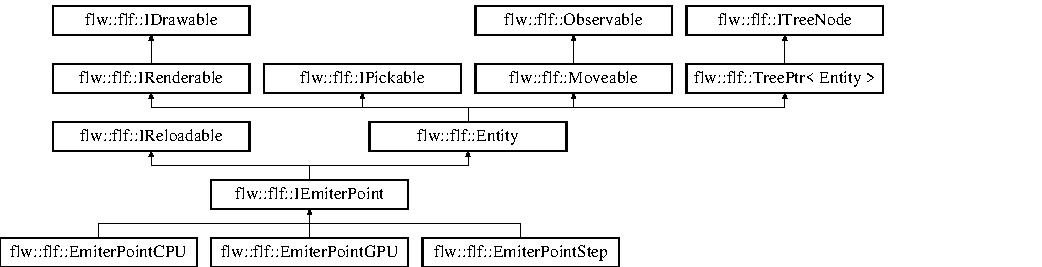
\includegraphics[height=3.589744cm]{classflw_1_1flf_1_1IEmiterPoint}
\end{center}
\end{figure}
\subsection*{Public Member Functions}
\begin{DoxyCompactItemize}
\item 
{\bfseries I\+Emiter\+Point} (\hyperlink{classflw_1_1Engine}{Engine} $\ast$engine, G\+Luint how\+Many, G\+Lfloat size, G\+Lfloat lifetime, \hyperlink{classflw_1_1flc_1_1Texture}{flc\+::\+Texture} $\ast$texture, glm\+::vec4 color, G\+Lenum blending\+Source, G\+Lenum blending\+Destination, G\+Lboolean depth\+Testing, G\+Lfloat alpha\+Cut\+Off)\hypertarget{classflw_1_1flf_1_1IEmiterPoint_a1f761af10d0b44e2847ea0f2150cdc0e}{}\label{classflw_1_1flf_1_1IEmiterPoint_a1f761af10d0b44e2847ea0f2150cdc0e}

\item 
void {\bfseries set\+Blending} (G\+Lenum source\+Factor, G\+Lenum destination\+Factor)\hypertarget{classflw_1_1flf_1_1IEmiterPoint_ad59e7a2e8b4559a54657638aa7249c8b}{}\label{classflw_1_1flf_1_1IEmiterPoint_ad59e7a2e8b4559a54657638aa7249c8b}

\item 
virtual void {\bfseries update} (G\+Lfloat time\+Elapsed\+Sec)=0\hypertarget{classflw_1_1flf_1_1IEmiterPoint_a7bfbe34cfbcf3222ab5e9068aedb3962}{}\label{classflw_1_1flf_1_1IEmiterPoint_a7bfbe34cfbcf3222ab5e9068aedb3962}

\item 
void {\bfseries draw} (\hyperlink{classflw_1_1flf_1_1ICamera}{I\+Camera} \&camera) override=0\hypertarget{classflw_1_1flf_1_1IEmiterPoint_aeffded615ab4356617b62556f6f13456}{}\label{classflw_1_1flf_1_1IEmiterPoint_aeffded615ab4356617b62556f6f13456}

\item 
void {\bfseries update\+Renderer} (\hyperlink{classflw_1_1flf_1_1IRenderer}{I\+Renderer} \&renderer) override\hypertarget{classflw_1_1flf_1_1IEmiterPoint_a1945d37be66cb8ef17f3f6d96f146dcc}{}\label{classflw_1_1flf_1_1IEmiterPoint_a1945d37be66cb8ef17f3f6d96f146dcc}

\end{DoxyCompactItemize}
\subsection*{Protected Attributes}
\begin{DoxyCompactItemize}
\item 
G\+Lfloat {\bfseries m\+Start\+Size}\hypertarget{classflw_1_1flf_1_1IEmiterPoint_a82128cd89b94e7d8bef15957bd2ecbd4}{}\label{classflw_1_1flf_1_1IEmiterPoint_a82128cd89b94e7d8bef15957bd2ecbd4}

\item 
G\+Lfloat {\bfseries m\+Lifetime}\hypertarget{classflw_1_1flf_1_1IEmiterPoint_a81255b1505630b745f025cc67c4ed6fc}{}\label{classflw_1_1flf_1_1IEmiterPoint_a81255b1505630b745f025cc67c4ed6fc}

\item 
\hyperlink{classflw_1_1flc_1_1Texture}{flc\+::\+Texture} $\ast$ {\bfseries m\+Texture}\hypertarget{classflw_1_1flf_1_1IEmiterPoint_ac2274b9022573a50a1c1b30cd259dc3f}{}\label{classflw_1_1flf_1_1IEmiterPoint_ac2274b9022573a50a1c1b30cd259dc3f}

\item 
glm\+::vec4 {\bfseries m\+Color}\hypertarget{classflw_1_1flf_1_1IEmiterPoint_afa54cf746b412ba2cfe60d5350f3a881}{}\label{classflw_1_1flf_1_1IEmiterPoint_afa54cf746b412ba2cfe60d5350f3a881}

\item 
G\+Luint {\bfseries m\+How\+Many}\hypertarget{classflw_1_1flf_1_1IEmiterPoint_afcabb90669a52d3076d2aa4e28d6b6d2}{}\label{classflw_1_1flf_1_1IEmiterPoint_afcabb90669a52d3076d2aa4e28d6b6d2}

\item 
G\+Lboolean {\bfseries m\+Depth\+Testing}\hypertarget{classflw_1_1flf_1_1IEmiterPoint_a64ffd2fbf1f0b93e83748a44c90fa0ed}{}\label{classflw_1_1flf_1_1IEmiterPoint_a64ffd2fbf1f0b93e83748a44c90fa0ed}

\item 
G\+Lfloat {\bfseries m\+Alpha\+Cut\+Off}\hypertarget{classflw_1_1flf_1_1IEmiterPoint_afd35bb053498b1bf4a736ff32b971983}{}\label{classflw_1_1flf_1_1IEmiterPoint_afd35bb053498b1bf4a736ff32b971983}

\item 
\hyperlink{classflw_1_1flc_1_1Program}{flc\+::\+Program} $\ast$ {\bfseries m\+Program}\hypertarget{classflw_1_1flf_1_1IEmiterPoint_ab31e42a70b7432ae87c10d0845f57c43}{}\label{classflw_1_1flf_1_1IEmiterPoint_ab31e42a70b7432ae87c10d0845f57c43}

\item 
\hyperlink{classflw_1_1flc_1_1IndexBuffer}{flc\+::\+Index\+Buffer} $\ast$ {\bfseries m\+I\+BO}\hypertarget{classflw_1_1flf_1_1IEmiterPoint_a6b2fea983d79268295f284f32df8b90e}{}\label{classflw_1_1flf_1_1IEmiterPoint_a6b2fea983d79268295f284f32df8b90e}

\item 
\hyperlink{structflw_1_1flf_1_1Blending}{Blending} {\bfseries m\+Blending}\hypertarget{classflw_1_1flf_1_1IEmiterPoint_a2afe359942465183b4fe614f55e631aa}{}\label{classflw_1_1flf_1_1IEmiterPoint_a2afe359942465183b4fe614f55e631aa}

\end{DoxyCompactItemize}
\subsection*{Additional Inherited Members}


\subsection{Detailed Description}
Drawable \hyperlink{classflw_1_1flf_1_1Entity}{Entity} which emits particles. 

The documentation for this class was generated from the following file\+:\begin{DoxyCompactItemize}
\item 
/home/filip/\+Projects/fillwave/inc/fillwave/models/base/I\+Emiter\+Point.\+h\end{DoxyCompactItemize}

\hypertarget{classflw_1_1flf_1_1IFocusable}{}\section{flw\+:\+:flf\+:\+:I\+Focusable Class Reference}
\label{classflw_1_1flf_1_1IFocusable}\index{flw\+::flf\+::\+I\+Focusable@{flw\+::flf\+::\+I\+Focusable}}


Capable to notify engine that focus related callbacks can be freed.  




{\ttfamily \#include $<$I\+Focusable.\+h$>$}

Inheritance diagram for flw\+:\+:flf\+:\+:I\+Focusable\+:\begin{figure}[H]
\begin{center}
\leavevmode
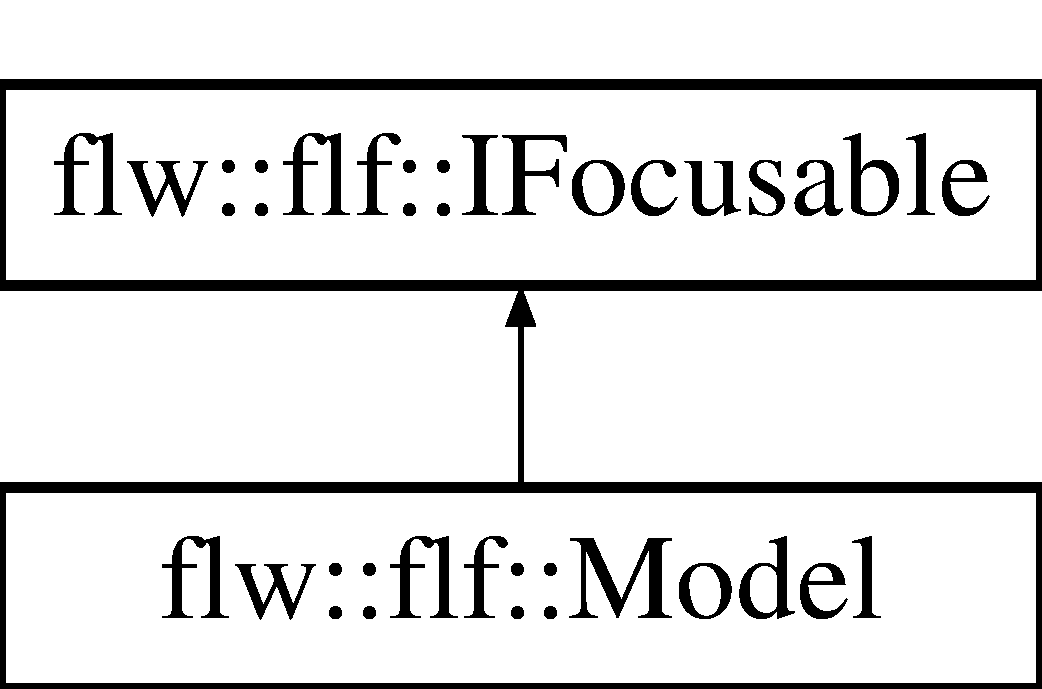
\includegraphics[height=2.000000cm]{classflw_1_1flf_1_1IFocusable}
\end{center}
\end{figure}
\subsection*{Public Member Functions}
\begin{DoxyCompactItemize}
\item 
{\bfseries I\+Focusable} (\hyperlink{classflw_1_1Engine}{Engine} $\ast$engine)\hypertarget{classflw_1_1flf_1_1IFocusable_ae388785b7481c5954481312b923bc4f1}{}\label{classflw_1_1flf_1_1IFocusable_ae388785b7481c5954481312b923bc4f1}

\item 
\hyperlink{classflw_1_1flf_1_1IFocusable}{I\+Focusable} \& {\bfseries operator=} (\hyperlink{classflw_1_1flf_1_1IFocusable}{I\+Focusable} \&\&)=default\hypertarget{classflw_1_1flf_1_1IFocusable_a1dd1b324b15e2bcfc123ccb6157eaa6a}{}\label{classflw_1_1flf_1_1IFocusable_a1dd1b324b15e2bcfc123ccb6157eaa6a}

\item 
{\bfseries I\+Focusable} (\hyperlink{classflw_1_1flf_1_1IFocusable}{I\+Focusable} \&\&obj)=default\hypertarget{classflw_1_1flf_1_1IFocusable_aab45eb8511a332d20b6887193bf90941}{}\label{classflw_1_1flf_1_1IFocusable_aab45eb8511a332d20b6887193bf90941}

\item 
virtual void {\bfseries handle\+Focus\+Event} (\hyperlink{classflw_1_1flf_1_1EventType}{Event\+Type} \&event)=0\hypertarget{classflw_1_1flf_1_1IFocusable_aea193ff346a8e7f6456dae0f9766fe31}{}\label{classflw_1_1flf_1_1IFocusable_aea193ff346a8e7f6456dae0f9766fe31}

\item 
void {\bfseries attach\+Callback} (\hyperlink{classflw_1_1flf_1_1Callback}{Callback} $\ast$callback)\hypertarget{classflw_1_1flf_1_1IFocusable_af8656575da10b5238cdcbe69697f09b3}{}\label{classflw_1_1flf_1_1IFocusable_af8656575da10b5238cdcbe69697f09b3}

\end{DoxyCompactItemize}
\subsection*{Protected Attributes}
\begin{DoxyCompactItemize}
\item 
\hyperlink{classflw_1_1Engine}{Engine} $\ast$ {\bfseries m\+Engine}\hypertarget{classflw_1_1flf_1_1IFocusable_a625d091b86ce2a676862a4dd603ffe8a}{}\label{classflw_1_1flf_1_1IFocusable_a625d091b86ce2a676862a4dd603ffe8a}

\item 
std\+::vector$<$ \hyperlink{classflw_1_1flf_1_1Callback}{Callback} $\ast$ $>$ {\bfseries m\+Callbacks}\hypertarget{classflw_1_1flf_1_1IFocusable_ab1e12a3db45e6f1ef06f661514103845}{}\label{classflw_1_1flf_1_1IFocusable_ab1e12a3db45e6f1ef06f661514103845}

\end{DoxyCompactItemize}


\subsection{Detailed Description}
Capable to notify engine that focus related callbacks can be freed. 

The documentation for this class was generated from the following file\+:\begin{DoxyCompactItemize}
\item 
/home/filip/\+Projects/fillwave/inc/fillwave/common/I\+Focusable.\+h\end{DoxyCompactItemize}

\hypertarget{classflw_1_1flf_1_1IHUDNode}{}\section{flw\+:\+:flf\+:\+:I\+H\+U\+D\+Node Class Reference}
\label{classflw_1_1flf_1_1IHUDNode}\index{flw\+::flf\+::\+I\+H\+U\+D\+Node@{flw\+::flf\+::\+I\+H\+U\+D\+Node}}


\hyperlink{classflw_1_1flf_1_1HUD}{H\+UD} base element.  




{\ttfamily \#include $<$I\+H\+U\+D\+Node.\+h$>$}

Inheritance diagram for flw\+:\+:flf\+:\+:I\+H\+U\+D\+Node\+:\begin{figure}[H]
\begin{center}
\leavevmode
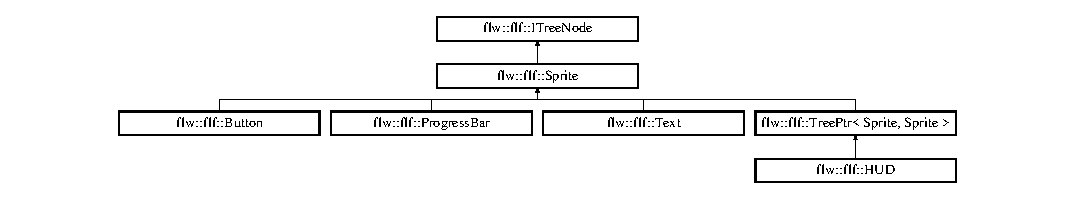
\includegraphics[height=2.222222cm]{classflw_1_1flf_1_1IHUDNode}
\end{center}
\end{figure}
\subsection*{Public Member Functions}
\begin{DoxyCompactItemize}
\item 
{\bfseries I\+H\+U\+D\+Node} (\hyperlink{classflw_1_1flc_1_1Texture2D}{flc\+::\+Texture2D} $\ast$texture=nullptr, \hyperlink{classflw_1_1flc_1_1Program}{flc\+::\+Program} $\ast$program=nullptr, glm\+::vec2 position=glm\+::vec2(0.\+0f, 0.\+0f), glm\+::vec2 scale=glm\+::vec2(1.\+0f, 1.\+0f))\hypertarget{classflw_1_1flf_1_1IHUDNode_a79410c95515a7f67e329f188a75eb2f1}{}\label{classflw_1_1flf_1_1IHUDNode_a79410c95515a7f67e329f188a75eb2f1}

\item 
virtual void {\bfseries draw} ()\hypertarget{classflw_1_1flf_1_1IHUDNode_a3b7f521fed9747d56cf8d7ee626c8c28}{}\label{classflw_1_1flf_1_1IHUDNode_a3b7f521fed9747d56cf8d7ee626c8c28}

\item 
void {\bfseries on\+Attached} (\hyperlink{classflw_1_1flf_1_1ITreeNode}{I\+Tree\+Node} $\ast$node) override\hypertarget{classflw_1_1flf_1_1IHUDNode_a36e5be05557f6daa4a7ef199fd1918e5}{}\label{classflw_1_1flf_1_1IHUDNode_a36e5be05557f6daa4a7ef199fd1918e5}

\item 
void {\bfseries on\+Detached} () override\hypertarget{classflw_1_1flf_1_1IHUDNode_a6979b712b6ef43ebffaf3419a670237f}{}\label{classflw_1_1flf_1_1IHUDNode_a6979b712b6ef43ebffaf3419a670237f}

\item 
void {\bfseries core\+Draw} ()\hypertarget{classflw_1_1flf_1_1IHUDNode_a744f438eb975e52fb88e28a12efc8411}{}\label{classflw_1_1flf_1_1IHUDNode_a744f438eb975e52fb88e28a12efc8411}

\end{DoxyCompactItemize}
\subsection*{Protected Attributes}
\begin{DoxyCompactItemize}
\item 
\hyperlink{classflw_1_1flc_1_1Texture2D}{flc\+::\+Texture2D} $\ast$ {\bfseries m\+Texture}\hypertarget{classflw_1_1flf_1_1IHUDNode_a71013ee08b9240d9d3c700820d9743f0}{}\label{classflw_1_1flf_1_1IHUDNode_a71013ee08b9240d9d3c700820d9743f0}

\item 
\hyperlink{classflw_1_1flc_1_1Program}{flc\+::\+Program} $\ast$ {\bfseries m\+Program}\hypertarget{classflw_1_1flf_1_1IHUDNode_a8a3d6ecd8d1b9d6d6b1843200e0d057e}{}\label{classflw_1_1flf_1_1IHUDNode_a8a3d6ecd8d1b9d6d6b1843200e0d057e}

\item 
glm\+::vec2 {\bfseries m\+Position}\hypertarget{classflw_1_1flf_1_1IHUDNode_aeea67115ea75ee618461914d139abdc5}{}\label{classflw_1_1flf_1_1IHUDNode_aeea67115ea75ee618461914d139abdc5}

\item 
glm\+::vec2 {\bfseries m\+Scale}\hypertarget{classflw_1_1flf_1_1IHUDNode_acbc889fbe0b0a77656c4764ee9e69458}{}\label{classflw_1_1flf_1_1IHUDNode_acbc889fbe0b0a77656c4764ee9e69458}

\item 
\hyperlink{structflw_1_1flf_1_1Blending}{Blending} {\bfseries m\+Blending}\hypertarget{classflw_1_1flf_1_1IHUDNode_a1ac47dfe7a7347beba350789870d4549}{}\label{classflw_1_1flf_1_1IHUDNode_a1ac47dfe7a7347beba350789870d4549}

\end{DoxyCompactItemize}


\subsection{Detailed Description}
\hyperlink{classflw_1_1flf_1_1HUD}{H\+UD} base element. 

The documentation for this class was generated from the following file\+:\begin{DoxyCompactItemize}
\item 
/home/filip/\+Projects/fillwave/inc/fillwave/hud/base/I\+H\+U\+D\+Node.\+h\end{DoxyCompactItemize}

\hypertarget{classflw_1_1flf_1_1Impostor}{}\section{flw\+:\+:flf\+:\+:Impostor Class Reference}
\label{classflw_1_1flf_1_1Impostor}\index{flw\+::flf\+::\+Impostor@{flw\+::flf\+::\+Impostor}}


Drawable \hyperlink{classflw_1_1flf_1_1Entity}{Entity} built by fragment shader. Time limited.  




{\ttfamily \#include $<$Impostor.\+h$>$}

Inheritance diagram for flw\+:\+:flf\+:\+:Impostor\+:\begin{figure}[H]
\begin{center}
\leavevmode
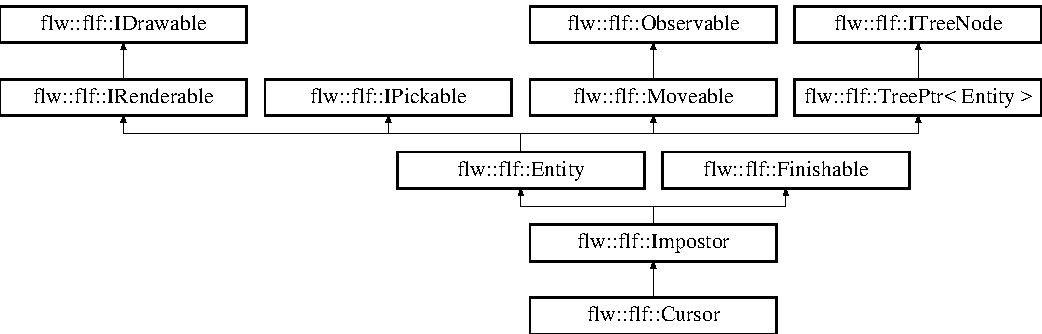
\includegraphics[height=4.487180cm]{classflw_1_1flf_1_1Impostor}
\end{center}
\end{figure}
\subsection*{Public Member Functions}
\begin{DoxyCompactItemize}
\item 
{\bfseries Impostor} (\hyperlink{classflw_1_1Engine}{Engine} $\ast$engine, G\+Lfloat lifetime, G\+Lfloat size, \hyperlink{classflw_1_1flc_1_1Texture}{flc\+::\+Texture} $\ast$texture=nullptr, G\+Lenum blending\+Source=G\+L\+\_\+\+S\+R\+C\+\_\+\+A\+L\+P\+HA, G\+Lenum blending\+Destination=G\+L\+\_\+\+O\+N\+E\+\_\+\+M\+I\+N\+U\+S\+\_\+\+S\+R\+C\+\_\+\+A\+L\+P\+HA)\hypertarget{classflw_1_1flf_1_1Impostor_a8e3518ed91a20cc188b1a216add6154f}{}\label{classflw_1_1flf_1_1Impostor_a8e3518ed91a20cc188b1a216add6154f}

\end{DoxyCompactItemize}
\subsection*{Protected Member Functions}
\begin{DoxyCompactItemize}
\item 
void {\bfseries core\+Draw} ()\hypertarget{classflw_1_1flf_1_1Impostor_a29d7972ad45278d2c45f55d28206a0b3}{}\label{classflw_1_1flf_1_1Impostor_a29d7972ad45278d2c45f55d28206a0b3}

\end{DoxyCompactItemize}
\subsection*{Protected Attributes}
\begin{DoxyCompactItemize}
\item 
\hyperlink{classflw_1_1flc_1_1Program}{flc\+::\+Program} $\ast$ {\bfseries m\+Program}\hypertarget{classflw_1_1flf_1_1Impostor_ac5fc51278468676481f5d26523b90aa6}{}\label{classflw_1_1flf_1_1Impostor_ac5fc51278468676481f5d26523b90aa6}

\item 
\hyperlink{classflw_1_1flc_1_1Texture}{flc\+::\+Texture} $\ast$ {\bfseries m\+Texture}\hypertarget{classflw_1_1flf_1_1Impostor_a79b817d46dd91909fc060ff0b557bde0}{}\label{classflw_1_1flf_1_1Impostor_a79b817d46dd91909fc060ff0b557bde0}

\item 
\hyperlink{classflw_1_1flc_1_1Sampler}{flc\+::\+Sampler} $\ast$ {\bfseries m\+Sampler}\hypertarget{classflw_1_1flf_1_1Impostor_abfec71be3aa6a5e08ae046f81484f0a3}{}\label{classflw_1_1flf_1_1Impostor_abfec71be3aa6a5e08ae046f81484f0a3}

\item 
G\+Lfloat {\bfseries m\+Size}\hypertarget{classflw_1_1flf_1_1Impostor_a3c0213e10db85ca55391c1629e82397a}{}\label{classflw_1_1flf_1_1Impostor_a3c0213e10db85ca55391c1629e82397a}

\item 
\hyperlink{structflw_1_1flf_1_1Blending}{Blending} {\bfseries m\+Blending}\hypertarget{classflw_1_1flf_1_1Impostor_a36c13287a923fc431368cf82f8d6d358}{}\label{classflw_1_1flf_1_1Impostor_a36c13287a923fc431368cf82f8d6d358}

\end{DoxyCompactItemize}
\subsection*{Additional Inherited Members}


\subsection{Detailed Description}
Drawable \hyperlink{classflw_1_1flf_1_1Entity}{Entity} built by fragment shader. Time limited. 

The documentation for this class was generated from the following file\+:\begin{DoxyCompactItemize}
\item 
/home/filip/\+Projects/fillwave/inc/fillwave/models/Impostor.\+h\end{DoxyCompactItemize}

\hypertarget{classflw_1_1flc_1_1IndexBuffer}{}\section{flw\+:\+:flc\+:\+:Index\+Buffer Class Reference}
\label{classflw_1_1flc_1_1IndexBuffer}\index{flw\+::flc\+::\+Index\+Buffer@{flw\+::flc\+::\+Index\+Buffer}}


Index\+Buffer\+Object -\/ I\+BO.  




{\ttfamily \#include $<$Index\+Buffer.\+h$>$}

Inheritance diagram for flw\+:\+:flc\+:\+:Index\+Buffer\+:\begin{figure}[H]
\begin{center}
\leavevmode
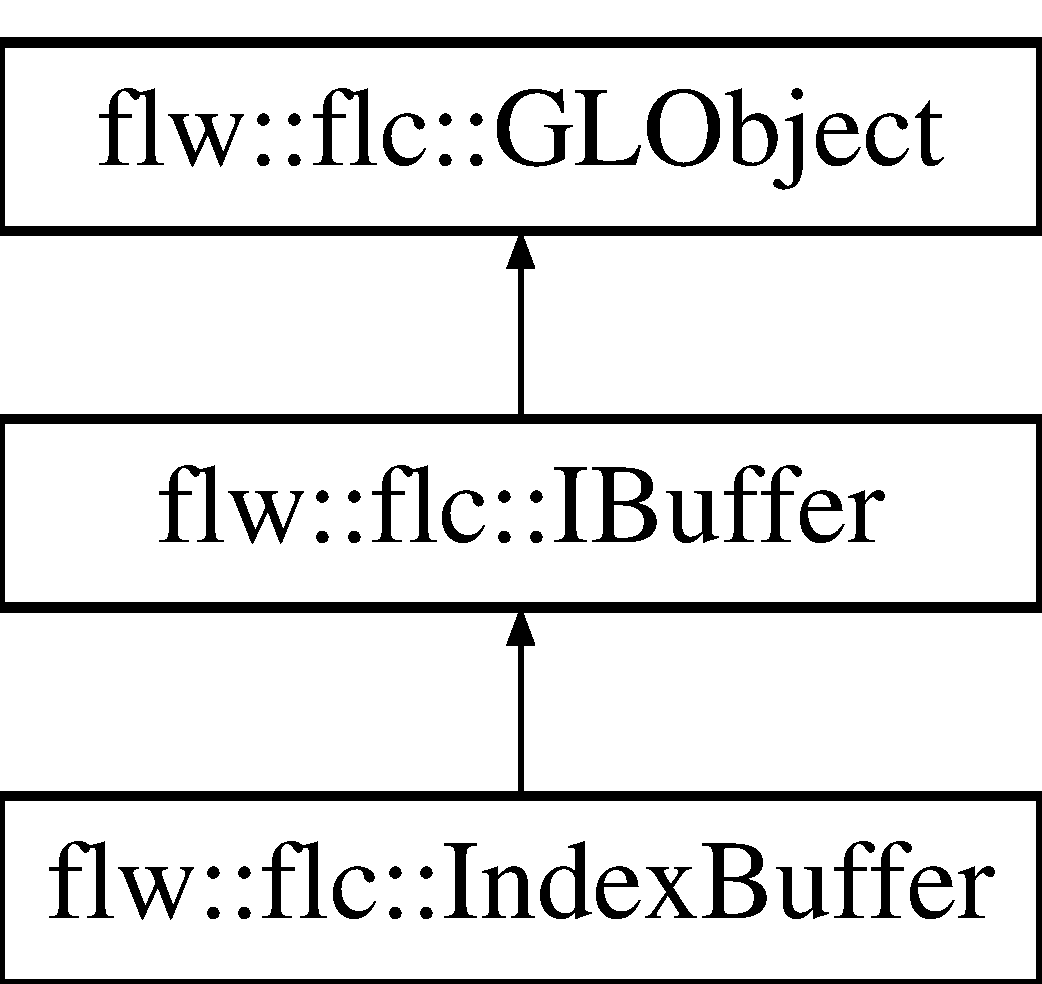
\includegraphics[height=3.000000cm]{classflw_1_1flc_1_1IndexBuffer}
\end{center}
\end{figure}
\subsection*{Public Member Functions}
\begin{DoxyCompactItemize}
\item 
\mbox{\Hypertarget{classflw_1_1flc_1_1IndexBuffer_a47991f0d3db10cfd1f946635e1a45aad}\label{classflw_1_1flc_1_1IndexBuffer_a47991f0d3db10cfd1f946635e1a45aad}} 
{\bfseries Index\+Buffer} (G\+Luint elements, bool fill, G\+Luint data\+Store\+Modification=G\+L\+\_\+\+S\+T\+A\+T\+I\+C\+\_\+\+D\+R\+AW)
\item 
\mbox{\Hypertarget{classflw_1_1flc_1_1IndexBuffer_a7bc7c0154f66f622e702830a1c005092}\label{classflw_1_1flc_1_1IndexBuffer_a7bc7c0154f66f622e702830a1c005092}} 
{\bfseries Index\+Buffer} (const std\+::vector$<$ G\+Luint $>$ \&data, G\+Luint data\+Store\+Modification=G\+L\+\_\+\+S\+T\+A\+T\+I\+C\+\_\+\+D\+R\+AW)
\item 
\mbox{\Hypertarget{classflw_1_1flc_1_1IndexBuffer_a9f5a8ec45b5f93f76eba01922cd76c90}\label{classflw_1_1flc_1_1IndexBuffer_a9f5a8ec45b5f93f76eba01922cd76c90}} 
G\+Luint $\ast$ {\bfseries get\+Data\+Internal} ()
\item 
\mbox{\Hypertarget{classflw_1_1flc_1_1IndexBuffer_a7dfedbdadc1a813955a25f1000f6c8c3}\label{classflw_1_1flc_1_1IndexBuffer_a7dfedbdadc1a813955a25f1000f6c8c3}} 
void {\bfseries empty\+C\+PU} () override
\item 
\mbox{\Hypertarget{classflw_1_1flc_1_1IndexBuffer_a88230425f7e4391a216acf45ffb2e1d0}\label{classflw_1_1flc_1_1IndexBuffer_a88230425f7e4391a216acf45ffb2e1d0}} 
void {\bfseries empty\+G\+PU} () override
\end{DoxyCompactItemize}
\subsection*{Protected Attributes}
\begin{DoxyCompactItemize}
\item 
\mbox{\Hypertarget{classflw_1_1flc_1_1IndexBuffer_a381007fe9db407c570104bdbd7f7d810}\label{classflw_1_1flc_1_1IndexBuffer_a381007fe9db407c570104bdbd7f7d810}} 
std\+::vector$<$ G\+Luint $>$ {\bfseries m\+Data\+Indices}
\end{DoxyCompactItemize}
\subsection*{Additional Inherited Members}


\subsection{Detailed Description}
Index\+Buffer\+Object -\/ I\+BO. 

The documentation for this class was generated from the following file\+:\begin{DoxyCompactItemize}
\item 
/home/filip/projects/fillwave/inc/fillwave/core/buffers/Index\+Buffer.\+h\end{DoxyCompactItemize}

\hypertarget{classflw_1_1flf_1_1IObserver}{}\section{flw\+:\+:flf\+:\+:I\+Observer Class Reference}
\label{classflw_1_1flf_1_1IObserver}\index{flw\+::flf\+::\+I\+Observer@{flw\+::flf\+::\+I\+Observer}}


Implementation of Observer pattern.  




{\ttfamily \#include $<$I\+Observer.\+h$>$}

Inheritance diagram for flw\+:\+:flf\+:\+:I\+Observer\+:\begin{figure}[H]
\begin{center}
\leavevmode
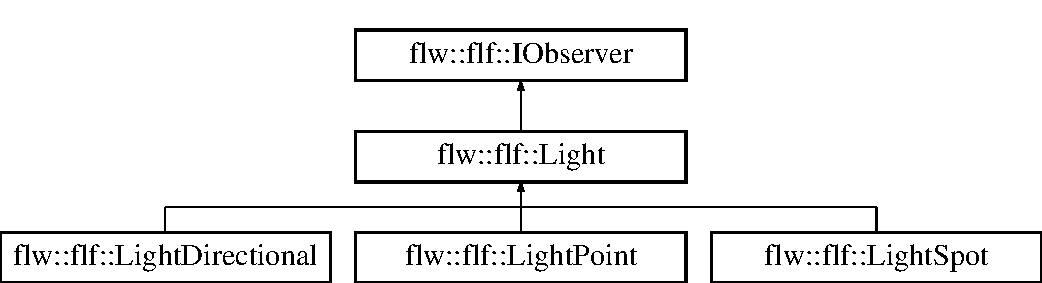
\includegraphics[height=3.000000cm]{classflw_1_1flf_1_1IObserver}
\end{center}
\end{figure}
\subsection*{Public Member Functions}
\begin{DoxyCompactItemize}
\item 
\mbox{\Hypertarget{classflw_1_1flf_1_1IObserver_ae87039fbfc41d947d3c6d945ae8004b9}\label{classflw_1_1flf_1_1IObserver_ae87039fbfc41d947d3c6d945ae8004b9}} 
virtual void {\bfseries on\+Death} (\hyperlink{classflw_1_1flf_1_1Observable}{Observable} $\ast$observable)=0
\item 
\mbox{\Hypertarget{classflw_1_1flf_1_1IObserver_a723ba4520e97e3602d01d70080092ea1}\label{classflw_1_1flf_1_1IObserver_a723ba4520e97e3602d01d70080092ea1}} 
virtual void {\bfseries on\+Changed} (\hyperlink{classflw_1_1flf_1_1Observable}{Observable} $\ast$observable)=0
\end{DoxyCompactItemize}


\subsection{Detailed Description}
Implementation of Observer pattern. 

The documentation for this class was generated from the following file\+:\begin{DoxyCompactItemize}
\item 
/home/filip/projects/fillwave/inc/fillwave/common/I\+Observer.\+h\end{DoxyCompactItemize}

\hypertarget{classflw_1_1flf_1_1IPickable}{}\section{flw\+:\+:flf\+:\+:I\+Pickable Class Reference}
\label{classflw_1_1flf_1_1IPickable}\index{flw\+::flf\+::\+I\+Pickable@{flw\+::flf\+::\+I\+Pickable}}


Pickable Interface.  




{\ttfamily \#include $<$I\+Pickable.\+h$>$}

Inheritance diagram for flw\+:\+:flf\+:\+:I\+Pickable\+:\begin{figure}[H]
\begin{center}
\leavevmode
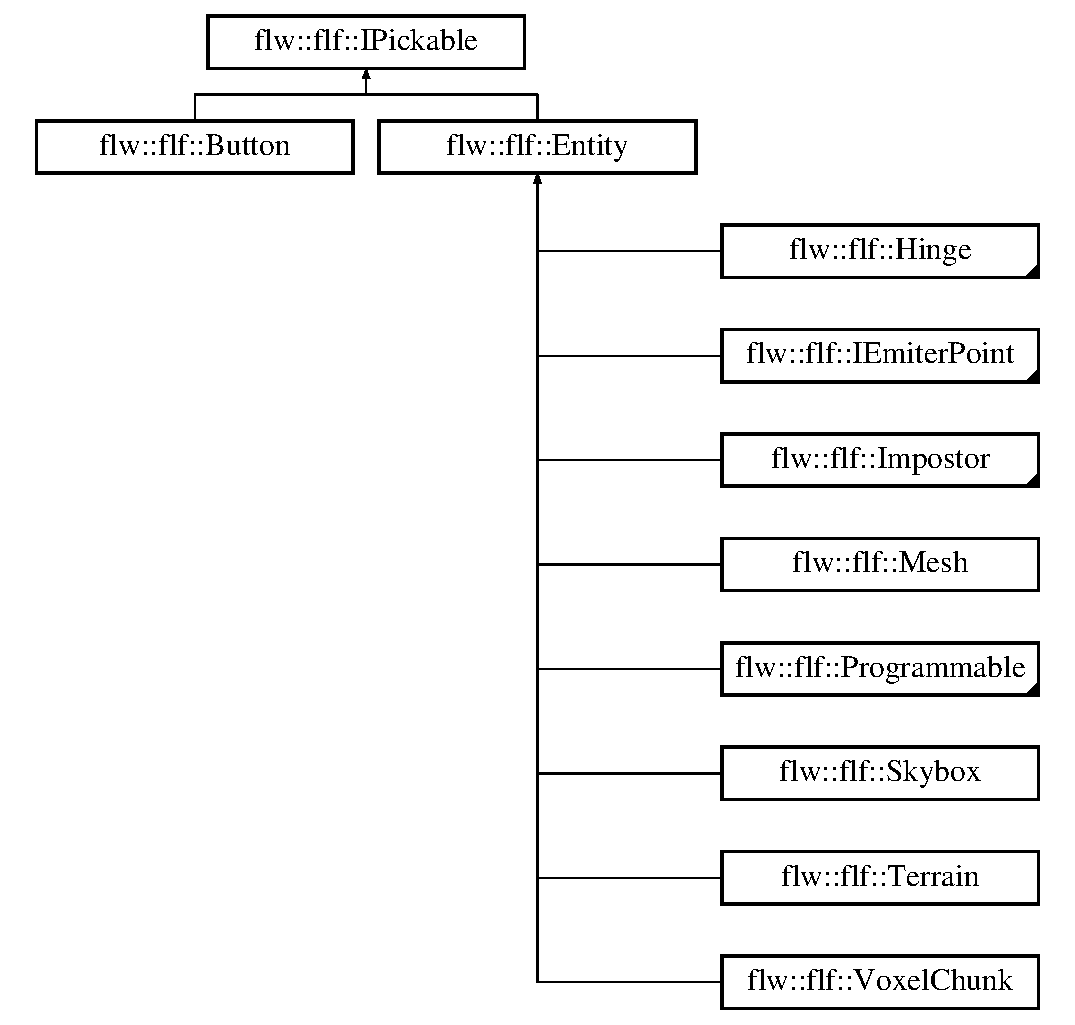
\includegraphics[height=10.000000cm]{classflw_1_1flf_1_1IPickable}
\end{center}
\end{figure}
\subsection*{Public Member Functions}
\begin{DoxyCompactItemize}
\item 
\mbox{\Hypertarget{classflw_1_1flf_1_1IPickable_ad5548ce0d61e0de87c326ca9996e4e63}\label{classflw_1_1flf_1_1IPickable_ad5548ce0d61e0de87c326ca9996e4e63}} 
\hyperlink{classflw_1_1flf_1_1IPickable}{I\+Pickable} \& {\bfseries operator=} (\hyperlink{classflw_1_1flf_1_1IPickable}{I\+Pickable} \&\&)=default
\item 
\mbox{\Hypertarget{classflw_1_1flf_1_1IPickable_a23026eef800645cb54962075284409d3}\label{classflw_1_1flf_1_1IPickable_a23026eef800645cb54962075284409d3}} 
{\bfseries I\+Pickable} (\hyperlink{classflw_1_1flf_1_1IPickable}{I\+Pickable} \&\&obj)=default
\item 
\mbox{\Hypertarget{classflw_1_1flf_1_1IPickable_a4314c9173e0cd472e7c4859cafdf9361}\label{classflw_1_1flf_1_1IPickable_a4314c9173e0cd472e7c4859cafdf9361}} 
bool {\bfseries is\+Pickable} ()
\item 
\mbox{\Hypertarget{classflw_1_1flf_1_1IPickable_a60a3e5e14ffc945860cb2d7d2d299cdd}\label{classflw_1_1flf_1_1IPickable_a60a3e5e14ffc945860cb2d7d2d299cdd}} 
glm\+::vec3 {\bfseries get\+Pickable\+Color} ()
\item 
\mbox{\Hypertarget{classflw_1_1flf_1_1IPickable_a979510a0522d576a2201c0b6f1139dd5}\label{classflw_1_1flf_1_1IPickable_a979510a0522d576a2201c0b6f1139dd5}} 
virtual void {\bfseries pick} (glm\+::vec3 color)=0
\item 
\mbox{\Hypertarget{classflw_1_1flf_1_1IPickable_a77481a6bd8396869c521667ae5204a48}\label{classflw_1_1flf_1_1IPickable_a77481a6bd8396869c521667ae5204a48}} 
virtual void {\bfseries unpick} ()=0
\item 
\mbox{\Hypertarget{classflw_1_1flf_1_1IPickable_aaa0dcbb8e0b550ce47c1aace8e277697}\label{classflw_1_1flf_1_1IPickable_aaa0dcbb8e0b550ce47c1aace8e277697}} 
virtual void {\bfseries on\+Picked} ()=0
\item 
\mbox{\Hypertarget{classflw_1_1flf_1_1IPickable_a98314352f99703305ac7ea382bf2ce2e}\label{classflw_1_1flf_1_1IPickable_a98314352f99703305ac7ea382bf2ce2e}} 
virtual void {\bfseries on\+Unpicked} ()=0
\end{DoxyCompactItemize}
\subsection*{Protected Attributes}
\begin{DoxyCompactItemize}
\item 
\mbox{\Hypertarget{classflw_1_1flf_1_1IPickable_adec6dd390430db763ad984910d609a97}\label{classflw_1_1flf_1_1IPickable_adec6dd390430db763ad984910d609a97}} 
bool {\bfseries m\+Flag\+Pickable}
\item 
\mbox{\Hypertarget{classflw_1_1flf_1_1IPickable_a4c5c7fc12317784810dce16a649be2d1}\label{classflw_1_1flf_1_1IPickable_a4c5c7fc12317784810dce16a649be2d1}} 
glm\+::vec3 {\bfseries m\+Pick\+Color}
\end{DoxyCompactItemize}


\subsection{Detailed Description}
Pickable Interface. 

The documentation for this class was generated from the following file\+:\begin{DoxyCompactItemize}
\item 
/home/filip/projects/fillwave/inc/fillwave/common/I\+Pickable.\+h\end{DoxyCompactItemize}

\hypertarget{classflw_1_1flf_1_1IReloadable}{}\section{flw\+:\+:flf\+:\+:I\+Reloadable Class Reference}
\label{classflw_1_1flf_1_1IReloadable}\index{flw\+::flf\+::\+I\+Reloadable@{flw\+::flf\+::\+I\+Reloadable}}


Encapsulates reloadable objects.  




{\ttfamily \#include $<$I\+Reloadable.\+h$>$}

Inheritance diagram for flw\+:\+:flf\+:\+:I\+Reloadable\+:\begin{figure}[H]
\begin{center}
\leavevmode
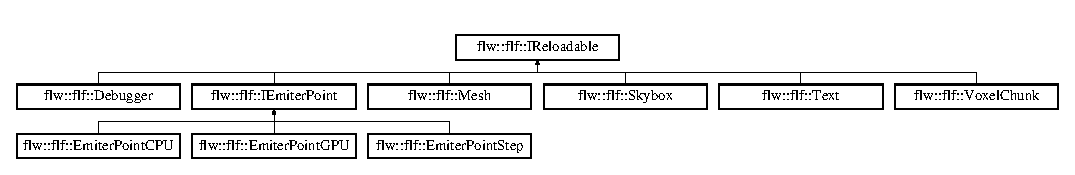
\includegraphics[height=1.904762cm]{classflw_1_1flf_1_1IReloadable}
\end{center}
\end{figure}
\subsection*{Public Member Functions}
\begin{DoxyCompactItemize}
\item 
\mbox{\Hypertarget{classflw_1_1flf_1_1IReloadable_ac731f61c6d138b0edcfaedbbfdaa532b}\label{classflw_1_1flf_1_1IReloadable_ac731f61c6d138b0edcfaedbbfdaa532b}} 
{\bfseries I\+Reloadable} (\hyperlink{classflw_1_1Engine}{Engine} $\ast$engine, \hyperlink{classflw_1_1flc_1_1VertexArray}{flc\+::\+Vertex\+Array} $\ast$=nullptr)
\item 
\mbox{\Hypertarget{classflw_1_1flf_1_1IReloadable_a8f95c0f4b89e86f07e5b84b920b52de5}\label{classflw_1_1flf_1_1IReloadable_a8f95c0f4b89e86f07e5b84b920b52de5}} 
virtual void {\bfseries init\+Buffers} ()=0
\item 
\mbox{\Hypertarget{classflw_1_1flf_1_1IReloadable_a955cc317fbf1e974c9721eba63d8b925}\label{classflw_1_1flf_1_1IReloadable_a955cc317fbf1e974c9721eba63d8b925}} 
virtual void {\bfseries init\+Pipeline} ()=0
\item 
\mbox{\Hypertarget{classflw_1_1flf_1_1IReloadable_aaa10b7aa64b43307022ea9c96a3745d5}\label{classflw_1_1flf_1_1IReloadable_aaa10b7aa64b43307022ea9c96a3745d5}} 
virtual void {\bfseries init\+Uniforms\+Cache} ()=0
\item 
\mbox{\Hypertarget{classflw_1_1flf_1_1IReloadable_ab7a74ae62026efd9a7c84285a2dda781}\label{classflw_1_1flf_1_1IReloadable_ab7a74ae62026efd9a7c84285a2dda781}} 
virtual void {\bfseries init\+V\+AO} ()=0
\item 
\mbox{\Hypertarget{classflw_1_1flf_1_1IReloadable_a93e45b66f1029e5fd95174b68fbc1114}\label{classflw_1_1flf_1_1IReloadable_a93e45b66f1029e5fd95174b68fbc1114}} 
virtual void {\bfseries init\+V\+BO} ()=0
\item 
\mbox{\Hypertarget{classflw_1_1flf_1_1IReloadable_a406820dd9f7ef66ca0df0dda52f666cd}\label{classflw_1_1flf_1_1IReloadable_a406820dd9f7ef66ca0df0dda52f666cd}} 
void {\bfseries reload} ()
\end{DoxyCompactItemize}
\subsection*{Protected Attributes}
\begin{DoxyCompactItemize}
\item 
\mbox{\Hypertarget{classflw_1_1flf_1_1IReloadable_a9aca34153ac7f3a633591234cd603e04}\label{classflw_1_1flf_1_1IReloadable_a9aca34153ac7f3a633591234cd603e04}} 
\hyperlink{classflw_1_1flc_1_1VertexArray}{flc\+::\+Vertex\+Array} $\ast$ {\bfseries m\+V\+AO}
\item 
\mbox{\Hypertarget{classflw_1_1flf_1_1IReloadable_ad7e7e8c96385b0bc2f6c65e8a18c7806}\label{classflw_1_1flf_1_1IReloadable_ad7e7e8c96385b0bc2f6c65e8a18c7806}} 
\hyperlink{classflw_1_1flc_1_1Sampler}{flc\+::\+Sampler} $\ast$ {\bfseries m\+Sampler}
\end{DoxyCompactItemize}


\subsection{Detailed Description}
Encapsulates reloadable objects. 

The documentation for this class was generated from the following file\+:\begin{DoxyCompactItemize}
\item 
/home/filip/projects/fillwave/inc/fillwave/models/base/I\+Reloadable.\+h\end{DoxyCompactItemize}

\hypertarget{classflw_1_1flf_1_1IRenderable}{}\section{flw\+:\+:flf\+:\+:I\+Renderable Class Reference}
\label{classflw_1_1flf_1_1IRenderable}\index{flw\+::flf\+::\+I\+Renderable@{flw\+::flf\+::\+I\+Renderable}}


Encapsulates renderable objects. To be used with \hyperlink{classflw_1_1flf_1_1IRenderer}{I\+Renderer}.  




{\ttfamily \#include $<$I\+Renderable.\+h$>$}

Inheritance diagram for flw\+:\+:flf\+:\+:I\+Renderable\+:\begin{figure}[H]
\begin{center}
\leavevmode
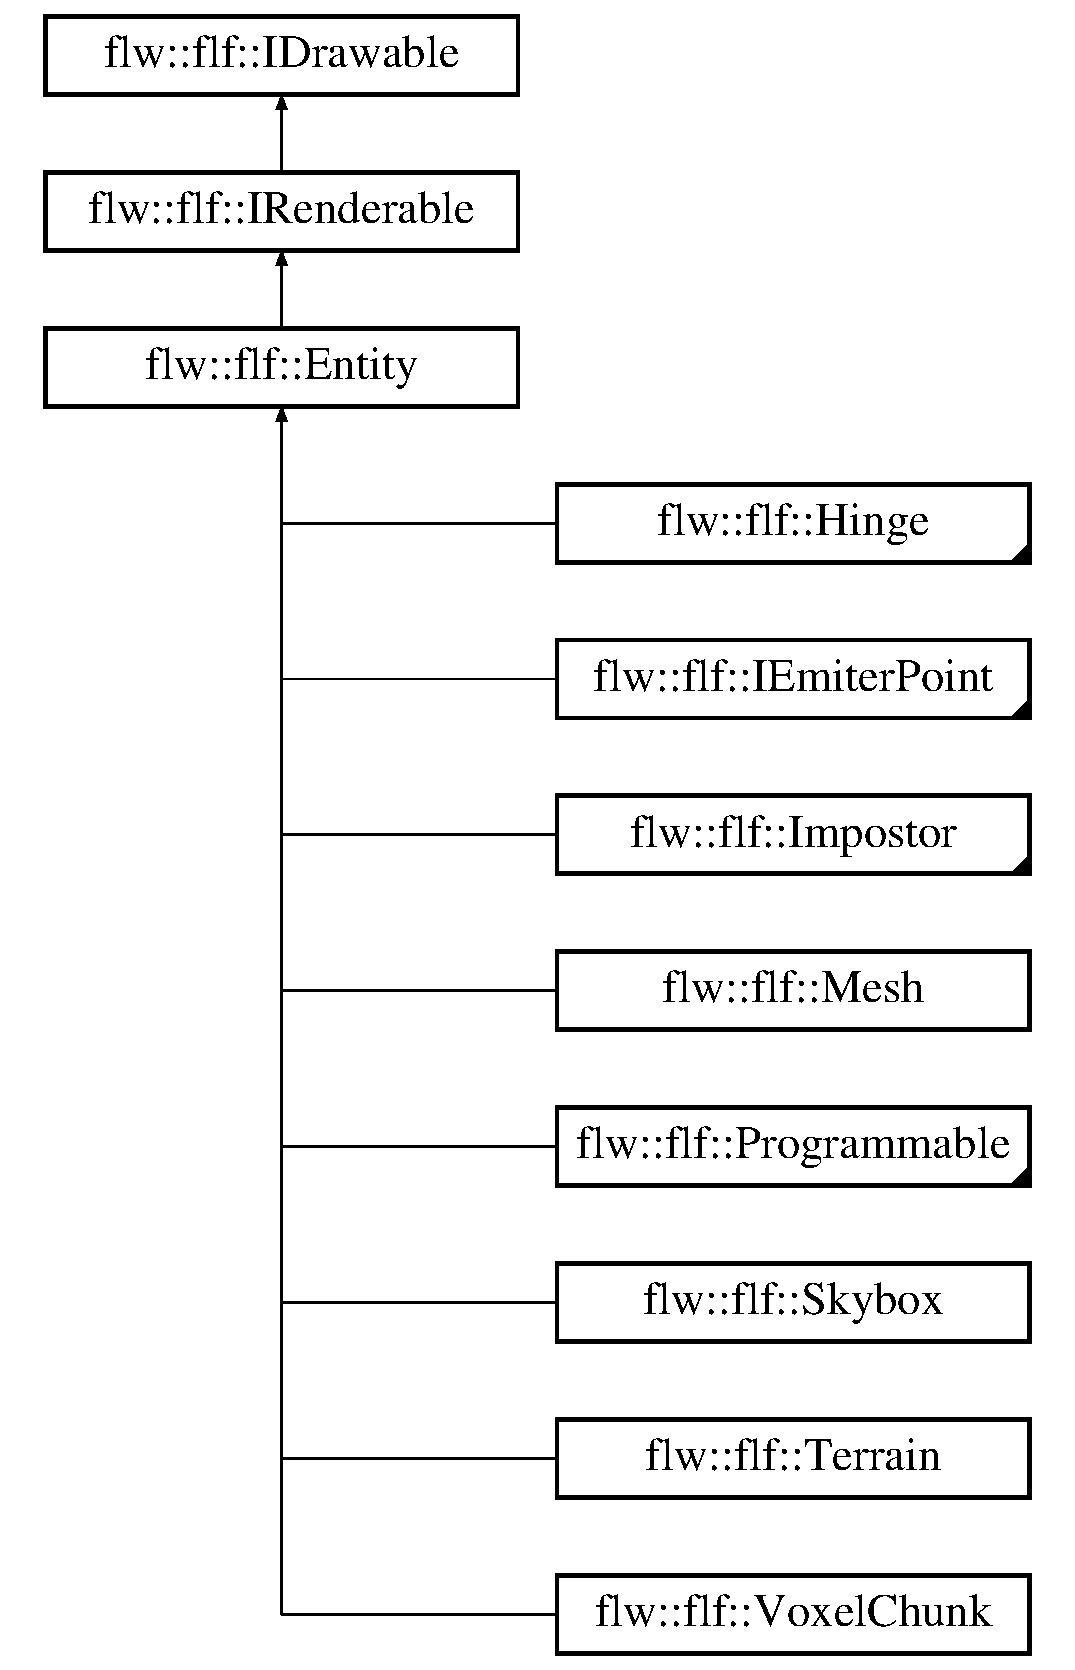
\includegraphics[height=11.000000cm]{classflw_1_1flf_1_1IRenderable}
\end{center}
\end{figure}
\subsection*{Public Member Functions}
\begin{DoxyCompactItemize}
\item 
virtual bool {\bfseries get\+Render\+Item} (\hyperlink{structflw_1_1flf_1_1RenderItem}{Render\+Item} \&item)=0\hypertarget{classflw_1_1flf_1_1IRenderable_a6605511b25801afe480d6c98af0394c8}{}\label{classflw_1_1flf_1_1IRenderable_a6605511b25801afe480d6c98af0394c8}

\item 
virtual void {\bfseries update\+Renderer} (\hyperlink{classflw_1_1flf_1_1IRenderer}{I\+Renderer} \&renderer)=0\hypertarget{classflw_1_1flf_1_1IRenderable_af31d698aaefd2171ce2efa1356c1e795}{}\label{classflw_1_1flf_1_1IRenderable_af31d698aaefd2171ce2efa1356c1e795}

\end{DoxyCompactItemize}


\subsection{Detailed Description}
Encapsulates renderable objects. To be used with \hyperlink{classflw_1_1flf_1_1IRenderer}{I\+Renderer}. 

The documentation for this class was generated from the following file\+:\begin{DoxyCompactItemize}
\item 
/home/filip/\+Projects/fillwave/inc/fillwave/models/base/I\+Renderable.\+h\end{DoxyCompactItemize}

\hypertarget{classflw_1_1flf_1_1IRenderer}{}\section{flw\+:\+:flf\+:\+:I\+Renderer Class Reference}
\label{classflw_1_1flf_1_1IRenderer}\index{flw\+::flf\+::\+I\+Renderer@{flw\+::flf\+::\+I\+Renderer}}


Base for all renderers.  




{\ttfamily \#include $<$I\+Renderer.\+h$>$}

Inheritance diagram for flw\+:\+:flf\+:\+:I\+Renderer\+:\begin{figure}[H]
\begin{center}
\leavevmode
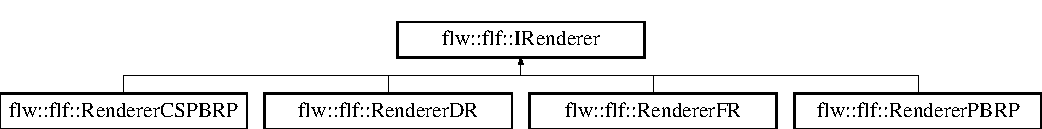
\includegraphics[height=1.739130cm]{classflw_1_1flf_1_1IRenderer}
\end{center}
\end{figure}
\subsection*{Public Member Functions}
\begin{DoxyCompactItemize}
\item 
virtual void {\bfseries update} (\hyperlink{classflw_1_1flf_1_1IRenderable}{I\+Renderable} $\ast$renderable)=0\hypertarget{classflw_1_1flf_1_1IRenderer_a3e7f0895caa92e95056be3404e28e788}{}\label{classflw_1_1flf_1_1IRenderer_a3e7f0895caa92e95056be3404e28e788}

\item 
virtual void {\bfseries draw} (\hyperlink{classflw_1_1flf_1_1ICamera}{I\+Camera} \&camera)=0\hypertarget{classflw_1_1flf_1_1IRenderer_a6b634d60f3fd4b6a28ec21cd7497208a}{}\label{classflw_1_1flf_1_1IRenderer_a6b634d60f3fd4b6a28ec21cd7497208a}

\item 
virtual void {\bfseries reset} (G\+Luint width, G\+Luint height)=0\hypertarget{classflw_1_1flf_1_1IRenderer_ac90ec601eac15ad54071f62078241c89}{}\label{classflw_1_1flf_1_1IRenderer_ac90ec601eac15ad54071f62078241c89}

\item 
virtual void {\bfseries clear} ()=0\hypertarget{classflw_1_1flf_1_1IRenderer_a425c79dae2088f55289aa69fabfa7bbe}{}\label{classflw_1_1flf_1_1IRenderer_a425c79dae2088f55289aa69fabfa7bbe}

\end{DoxyCompactItemize}
\subsection*{Public Attributes}
\begin{DoxyCompactItemize}
\item 
bool {\bfseries m\+Flag\+Reload}\hypertarget{classflw_1_1flf_1_1IRenderer_aefe02e2d025ff1ce6e7553c2c1f9b7fa}{}\label{classflw_1_1flf_1_1IRenderer_aefe02e2d025ff1ce6e7553c2c1f9b7fa}

\item 
\hyperlink{classflw_1_1flf_1_1Skybox}{Skybox} $\ast$ {\bfseries m\+Skybox}\hypertarget{classflw_1_1flf_1_1IRenderer_a14ec6383fdb9e4edcc8c27d4290c4cdd}{}\label{classflw_1_1flf_1_1IRenderer_a14ec6383fdb9e4edcc8c27d4290c4cdd}

\item 
G\+Lfloat {\bfseries m\+Ambient\+Global} \mbox{[}3\mbox{]}\hypertarget{classflw_1_1flf_1_1IRenderer_a3e09bfcf3e5c8c6c42dd40b782b7906f}{}\label{classflw_1_1flf_1_1IRenderer_a3e09bfcf3e5c8c6c42dd40b782b7906f}

\end{DoxyCompactItemize}


\subsection{Detailed Description}
Base for all renderers. 

The documentation for this class was generated from the following file\+:\begin{DoxyCompactItemize}
\item 
/home/filip/\+Projects/fillwave/inc/fillwave/renderers/I\+Renderer.\+h\end{DoxyCompactItemize}

\hypertarget{classflw_1_1flf_1_1ITreeNode}{}\section{flw\+:\+:flf\+:\+:I\+Tree\+Node Class Reference}
\label{classflw_1_1flf_1_1ITreeNode}\index{flw\+::flf\+::\+I\+Tree\+Node@{flw\+::flf\+::\+I\+Tree\+Node}}


Basic tree \hyperlink{classflw_1_1flf_1_1ITreeNode}{I\+Tree\+Node} Interface.  




{\ttfamily \#include $<$I\+Tree\+Node.\+h$>$}

Inheritance diagram for flw\+:\+:flf\+:\+:I\+Tree\+Node\+:\begin{figure}[H]
\begin{center}
\leavevmode
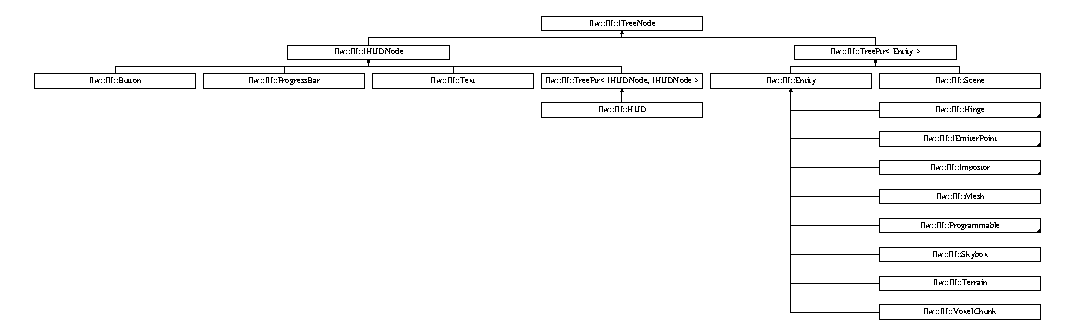
\includegraphics[height=4.074074cm]{classflw_1_1flf_1_1ITreeNode}
\end{center}
\end{figure}
\subsection*{Public Member Functions}
\begin{DoxyCompactItemize}
\item 
virtual void {\bfseries on\+Attached} (\hyperlink{classflw_1_1flf_1_1ITreeNode}{I\+Tree\+Node} $\ast$parent)=0\hypertarget{classflw_1_1flf_1_1ITreeNode_a983181e4935b547e38b7234410324f90}{}\label{classflw_1_1flf_1_1ITreeNode_a983181e4935b547e38b7234410324f90}

\item 
virtual void {\bfseries on\+Detached} ()=0\hypertarget{classflw_1_1flf_1_1ITreeNode_a2452e98a3718088c87993ac30735f190}{}\label{classflw_1_1flf_1_1ITreeNode_a2452e98a3718088c87993ac30735f190}

\end{DoxyCompactItemize}


\subsection{Detailed Description}
Basic tree \hyperlink{classflw_1_1flf_1_1ITreeNode}{I\+Tree\+Node} Interface. 

The documentation for this class was generated from the following file\+:\begin{DoxyCompactItemize}
\item 
/home/filip/\+Projects/fillwave/inc/fillwave/models/base/I\+Tree\+Node.\+h\end{DoxyCompactItemize}

\hypertarget{classflw_1_1flf_1_1Key}{}\section{flw\+:\+:flf\+:\+:Key$<$ T $>$ Class Template Reference}
\label{classflw_1_1flf_1_1Key}\index{flw\+::flf\+::\+Key$<$ T $>$@{flw\+::flf\+::\+Key$<$ T $>$}}


Base for all animation keys.  




{\ttfamily \#include $<$Key.\+h$>$}

\subsection*{Public Member Functions}
\begin{DoxyCompactItemize}
\item 
\mbox{\Hypertarget{classflw_1_1flf_1_1Key_a28b10bc048b2761a3e34566e0139111c}\label{classflw_1_1flf_1_1Key_a28b10bc048b2761a3e34566e0139111c}} 
{\bfseries Key} (float time\+Stamp, T value)
\end{DoxyCompactItemize}
\subsection*{Public Attributes}
\begin{DoxyCompactItemize}
\item 
\mbox{\Hypertarget{classflw_1_1flf_1_1Key_a935d2e69a4f83e9fbb811069ed38158d}\label{classflw_1_1flf_1_1Key_a935d2e69a4f83e9fbb811069ed38158d}} 
float {\bfseries m\+Time}
\item 
\mbox{\Hypertarget{classflw_1_1flf_1_1Key_aba66088ad43b89c391feaf4769d58836}\label{classflw_1_1flf_1_1Key_aba66088ad43b89c391feaf4769d58836}} 
T {\bfseries m\+Value}
\end{DoxyCompactItemize}


\subsection{Detailed Description}
\subsubsection*{template$<$class T$>$\newline
class flw\+::flf\+::\+Key$<$ T $>$}

Base for all animation keys. 

The documentation for this class was generated from the following file\+:\begin{DoxyCompactItemize}
\item 
/home/filip/projects/fillwave/inc/fillwave/models/animations/Key.\+h\end{DoxyCompactItemize}

\hypertarget{classflw_1_1flf_1_1KeyboardEvent}{}\section{flw\+:\+:flf\+:\+:Keyboard\+Event Struct Reference}
\label{classflw_1_1flf_1_1KeyboardEvent}\index{flw\+::flf\+::\+Keyboard\+Event@{flw\+::flf\+::\+Keyboard\+Event}}


Event introduced when something happens with the key.  




{\ttfamily \#include $<$Keyboard\+T\+Event.\+h$>$}

Inheritance diagram for flw\+:\+:flf\+:\+:Keyboard\+Event\+:\begin{figure}[H]
\begin{center}
\leavevmode
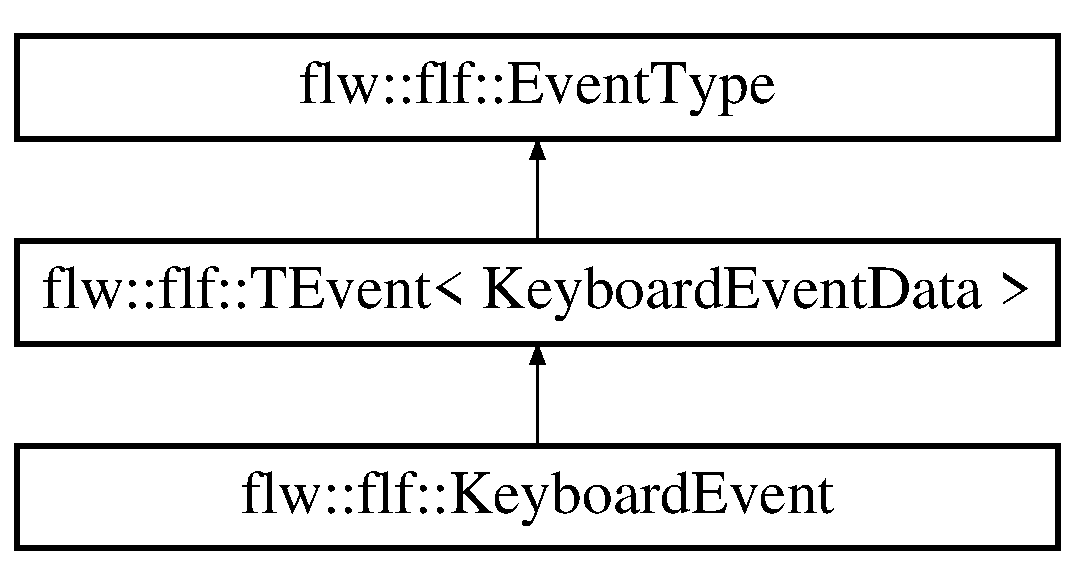
\includegraphics[height=3.000000cm]{classflw_1_1flf_1_1KeyboardEvent}
\end{center}
\end{figure}
\subsection*{Public Member Functions}
\begin{DoxyCompactItemize}
\item 
{\bfseries Keyboard\+Event} (\hyperlink{structflw_1_1flf_1_1KeyboardEventData}{Keyboard\+Event\+Data} data)\hypertarget{classflw_1_1flf_1_1KeyboardEvent_a9b9b33118361421d25568fe9d79985e4}{}\label{classflw_1_1flf_1_1KeyboardEvent_a9b9b33118361421d25568fe9d79985e4}

\end{DoxyCompactItemize}
\subsection*{Additional Inherited Members}


\subsection{Detailed Description}
Event introduced when something happens with the key. 

The documentation for this struct was generated from the following file\+:\begin{DoxyCompactItemize}
\item 
/home/filip/\+Projects/fillwave/inc/fillwave/actions/events/Keyboard\+T\+Event.\+h\end{DoxyCompactItemize}

\hypertarget{structflw_1_1flf_1_1KeyboardEventData}{}\section{flw\+:\+:flf\+:\+:Keyboard\+Event\+Data Struct Reference}
\label{structflw_1_1flf_1_1KeyboardEventData}\index{flw\+::flf\+::\+Keyboard\+Event\+Data@{flw\+::flf\+::\+Keyboard\+Event\+Data}}


Event data structure to store the parameters of a key event.  




{\ttfamily \#include $<$Keyboard\+T\+Event.\+h$>$}

\subsection*{Public Attributes}
\begin{DoxyCompactItemize}
\item 
int {\bfseries key}\hypertarget{structflw_1_1flf_1_1KeyboardEventData_a2eee2bc4f3f58cdf4009b0677dacd0cc}{}\label{structflw_1_1flf_1_1KeyboardEventData_a2eee2bc4f3f58cdf4009b0677dacd0cc}

\item 
int {\bfseries scan\+Code}\hypertarget{structflw_1_1flf_1_1KeyboardEventData_acd8697357c1dcfeca37bda6b6ba19eee}{}\label{structflw_1_1flf_1_1KeyboardEventData_acd8697357c1dcfeca37bda6b6ba19eee}

\item 
int {\bfseries action}\hypertarget{structflw_1_1flf_1_1KeyboardEventData_a306c515779fc9bf90b019a4fe4a51b97}{}\label{structflw_1_1flf_1_1KeyboardEventData_a306c515779fc9bf90b019a4fe4a51b97}

\item 
int {\bfseries mode}\hypertarget{structflw_1_1flf_1_1KeyboardEventData_a022d96d5b0d3c683193e0ad1afbe39ef}{}\label{structflw_1_1flf_1_1KeyboardEventData_a022d96d5b0d3c683193e0ad1afbe39ef}

\item 
const e\+Event\+Type {\bfseries type} = e\+Event\+Type\+::e\+Key\hypertarget{structflw_1_1flf_1_1KeyboardEventData_acc0cc77adf02ddae2f0dc1b340b82a1c}{}\label{structflw_1_1flf_1_1KeyboardEventData_acc0cc77adf02ddae2f0dc1b340b82a1c}

\end{DoxyCompactItemize}


\subsection{Detailed Description}
Event data structure to store the parameters of a key event. 

The documentation for this struct was generated from the following file\+:\begin{DoxyCompactItemize}
\item 
/home/filip/\+Projects/fillwave/inc/fillwave/actions/events/Keyboard\+T\+Event.\+h\end{DoxyCompactItemize}

\hypertarget{classflw_1_1flf_1_1Light}{}\section{flw\+:\+:flf\+:\+:Light Class Reference}
\label{classflw_1_1flf_1_1Light}\index{flw\+::flf\+::\+Light@{flw\+::flf\+::\+Light}}


Base for all lights.  




{\ttfamily \#include $<$Light.\+h$>$}

Inheritance diagram for flw\+:\+:flf\+:\+:Light\+:\begin{figure}[H]
\begin{center}
\leavevmode
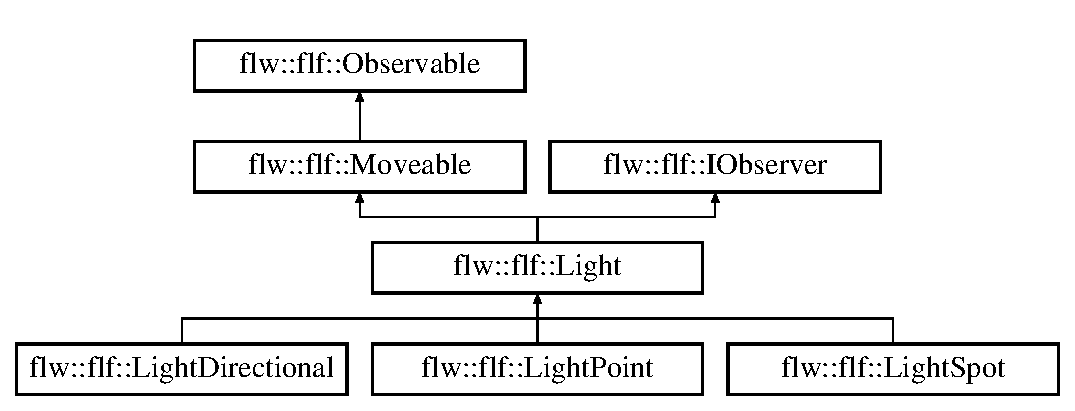
\includegraphics[height=4.000000cm]{classflw_1_1flf_1_1Light}
\end{center}
\end{figure}
\subsection*{Public Member Functions}
\begin{DoxyCompactItemize}
\item 
\mbox{\Hypertarget{classflw_1_1flf_1_1Light_a36084a4a54fad153bf47c7c3c4759809}\label{classflw_1_1flf_1_1Light_a36084a4a54fad153bf47c7c3c4759809}} 
{\bfseries Light} (glm\+::vec3 position, glm\+::vec4 intensity, \hyperlink{classflw_1_1flf_1_1Moveable}{Moveable} $\ast$followed)
\item 
\mbox{\Hypertarget{classflw_1_1flf_1_1Light_a66488fb86f264c9b9235880f43068d79}\label{classflw_1_1flf_1_1Light_a66488fb86f264c9b9235880f43068d79}} 
void {\bfseries update\+From\+Followed} ()
\item 
\mbox{\Hypertarget{classflw_1_1flf_1_1Light_a36e8aa7f8645aefb2ab4ec6d54895158}\label{classflw_1_1flf_1_1Light_a36e8aa7f8645aefb2ab4ec6d54895158}} 
void {\bfseries set\+Attenuation} (\hyperlink{structflw_1_1flf_1_1LightAttenuationData}{Light\+Attenuation\+Data} \&attenuation)
\item 
\mbox{\Hypertarget{classflw_1_1flf_1_1Light_aa057776a1eb1796978ebcd334574f1de}\label{classflw_1_1flf_1_1Light_aa057776a1eb1796978ebcd334574f1de}} 
\hyperlink{structflw_1_1flf_1_1LightAttenuationData}{Light\+Attenuation\+Data} {\bfseries get\+Attenuation} ()
\item 
\mbox{\Hypertarget{classflw_1_1flf_1_1Light_a1d8e6e0e191a3c47a3ea87a62445d89c}\label{classflw_1_1flf_1_1Light_a1d8e6e0e191a3c47a3ea87a62445d89c}} 
void {\bfseries set\+Intensity} (glm\+::vec4 intensity)
\item 
\mbox{\Hypertarget{classflw_1_1flf_1_1Light_aadb91107eef0e1e24363a2b757e649e1}\label{classflw_1_1flf_1_1Light_aadb91107eef0e1e24363a2b757e649e1}} 
glm\+::vec4 {\bfseries get\+Intensity} ()
\item 
\mbox{\Hypertarget{classflw_1_1flf_1_1Light_ac5313d3d1b9a37f486aae0de56bccaa0}\label{classflw_1_1flf_1_1Light_ac5313d3d1b9a37f486aae0de56bccaa0}} 
void {\bfseries log} ()
\item 
\mbox{\Hypertarget{classflw_1_1flf_1_1Light_a818069ca94cb8932324eea986146a7f0}\label{classflw_1_1flf_1_1Light_a818069ca94cb8932324eea986146a7f0}} 
void {\bfseries on\+Death} (\hyperlink{classflw_1_1flf_1_1Observable}{Observable} $\ast$observable) override
\item 
\mbox{\Hypertarget{classflw_1_1flf_1_1Light_a150573245975df8e0e436f590c85d239}\label{classflw_1_1flf_1_1Light_a150573245975df8e0e436f590c85d239}} 
void {\bfseries on\+Changed} (\hyperlink{classflw_1_1flf_1_1Observable}{Observable} $\ast$observable) override
\end{DoxyCompactItemize}
\subsection*{Protected Attributes}
\begin{DoxyCompactItemize}
\item 
\mbox{\Hypertarget{classflw_1_1flf_1_1Light_a4f186929fcf2f2de8e22b55c72e68524}\label{classflw_1_1flf_1_1Light_a4f186929fcf2f2de8e22b55c72e68524}} 
\hyperlink{classflw_1_1flf_1_1Moveable}{Moveable} $\ast$ {\bfseries m\+Followed}
\item 
\mbox{\Hypertarget{classflw_1_1flf_1_1Light_a19d2713688b231ecea3ed8ffefe5d61f}\label{classflw_1_1flf_1_1Light_a19d2713688b231ecea3ed8ffefe5d61f}} 
bool {\bfseries m\+Is\+Followed\+Updated}
\item 
\mbox{\Hypertarget{classflw_1_1flf_1_1Light_a45fd5157caf2cd94b8d2756b776f7232}\label{classflw_1_1flf_1_1Light_a45fd5157caf2cd94b8d2756b776f7232}} 
glm\+::vec4 {\bfseries m\+Intensity}
\item 
\mbox{\Hypertarget{classflw_1_1flf_1_1Light_a095fa4c4d6b253e829711dc449e7b302}\label{classflw_1_1flf_1_1Light_a095fa4c4d6b253e829711dc449e7b302}} 
\hyperlink{structflw_1_1flf_1_1LightAttenuationData}{Light\+Attenuation\+Data} {\bfseries m\+Attenuation}
\end{DoxyCompactItemize}


\subsection{Detailed Description}
Base for all lights. 

The documentation for this class was generated from the following file\+:\begin{DoxyCompactItemize}
\item 
/home/filip/projects/fillwave/inc/fillwave/space/base/Light.\+h\end{DoxyCompactItemize}

\hypertarget{structflw_1_1flf_1_1LightAttenuationData}{}\section{flw\+:\+:flf\+:\+:Light\+Attenuation\+Data Struct Reference}
\label{structflw_1_1flf_1_1LightAttenuationData}\index{flw\+::flf\+::\+Light\+Attenuation\+Data@{flw\+::flf\+::\+Light\+Attenuation\+Data}}


\hyperlink{classflw_1_1flf_1_1Light}{Light} attenuation data.  




{\ttfamily \#include $<$Light.\+h$>$}

\subsection*{Public Attributes}
\begin{DoxyCompactItemize}
\item 
G\+Lfloat {\bfseries m\+Linear}\hypertarget{structflw_1_1flf_1_1LightAttenuationData_af36466eb7114528901c5e29268e1a771}{}\label{structflw_1_1flf_1_1LightAttenuationData_af36466eb7114528901c5e29268e1a771}

\item 
G\+Lfloat {\bfseries m\+Exp}\hypertarget{structflw_1_1flf_1_1LightAttenuationData_ac30bbb96fe369514c57d71b282b51708}{}\label{structflw_1_1flf_1_1LightAttenuationData_ac30bbb96fe369514c57d71b282b51708}

\end{DoxyCompactItemize}


\subsection{Detailed Description}
\hyperlink{classflw_1_1flf_1_1Light}{Light} attenuation data. 

The documentation for this struct was generated from the following file\+:\begin{DoxyCompactItemize}
\item 
/home/filip/\+Projects/fillwave/inc/fillwave/space/base/Light.\+h\end{DoxyCompactItemize}

\hypertarget{structflw_1_1flf_1_1LightDirectioData}{}\section{flw\+:\+:flf\+:\+:Light\+Directio\+Data Struct Reference}
\label{structflw_1_1flf_1_1LightDirectioData}\index{flw\+::flf\+::\+Light\+Directio\+Data@{flw\+::flf\+::\+Light\+Directio\+Data}}


\hyperlink{classflw_1_1flf_1_1Light}{Light} U\+BO data.  




{\ttfamily \#include $<$Light\+Directional.\+h$>$}

\subsection*{Public Attributes}
\begin{DoxyCompactItemize}
\item 
G\+Lfloat {\bfseries position} \mbox{[}4\mbox{]}\hypertarget{structflw_1_1flf_1_1LightDirectioData_ab93fd8912e661b05321da657edf5e2b8}{}\label{structflw_1_1flf_1_1LightDirectioData_ab93fd8912e661b05321da657edf5e2b8}

\item 
G\+Lfloat {\bfseries intensity} \mbox{[}4\mbox{]}\hypertarget{structflw_1_1flf_1_1LightDirectioData_ad3d310df515162775577c730388ae561}{}\label{structflw_1_1flf_1_1LightDirectioData_ad3d310df515162775577c730388ae561}

\item 
G\+Lfloat {\bfseries mvp} \mbox{[}16\mbox{]}\hypertarget{structflw_1_1flf_1_1LightDirectioData_ad0792b0c7715fa130dfa0aecfed8b5db}{}\label{structflw_1_1flf_1_1LightDirectioData_ad0792b0c7715fa130dfa0aecfed8b5db}

\end{DoxyCompactItemize}


\subsection{Detailed Description}
\hyperlink{classflw_1_1flf_1_1Light}{Light} U\+BO data. 

The documentation for this struct was generated from the following file\+:\begin{DoxyCompactItemize}
\item 
/home/filip/\+Projects/fillwave/inc/fillwave/space/Light\+Directional.\+h\end{DoxyCompactItemize}

\hypertarget{classflw_1_1flf_1_1LightDirectional}{}\section{flw\+:\+:flf\+:\+:Light\+Directional Class Reference}
\label{classflw_1_1flf_1_1LightDirectional}\index{flw\+::flf\+::\+Light\+Directional@{flw\+::flf\+::\+Light\+Directional}}


\hyperlink{classflw_1_1flf_1_1Light}{Light} with Orthographic projection.  




{\ttfamily \#include $<$Light\+Directional.\+h$>$}

Inheritance diagram for flw\+:\+:flf\+:\+:Light\+Directional\+:\begin{figure}[H]
\begin{center}
\leavevmode
\includegraphics[height=4.000000cm]{classflw_1_1flf_1_1LightDirectional}
\end{center}
\end{figure}
\subsection*{Public Member Functions}
\begin{DoxyCompactItemize}
\item 
\mbox{\Hypertarget{classflw_1_1flf_1_1LightDirectional_a09b4fc109a231d81fccf59834abb1d92}\label{classflw_1_1flf_1_1LightDirectional_a09b4fc109a231d81fccf59834abb1d92}} 
{\bfseries Light\+Directional} (\hyperlink{classflw_1_1flc_1_1Texture2DRenderable}{flc\+::\+Texture2\+D\+Renderable} $\ast$shadow\+Texture, glm\+::vec3 position, glm\+::quat rotation, glm\+::vec4 intensity, \hyperlink{classflw_1_1flf_1_1Moveable}{Moveable} $\ast$followed=nullptr)
\item 
\mbox{\Hypertarget{classflw_1_1flf_1_1LightDirectional_af5551815e42ffc40f2c6e0062effa783}\label{classflw_1_1flf_1_1LightDirectional_af5551815e42ffc40f2c6e0062effa783}} 
\hyperlink{classflw_1_1flc_1_1Texture2DRenderable}{flc\+::\+Texture2\+D\+Renderable} $\ast$ {\bfseries get\+Shadow\+Texture} ()
\item 
\mbox{\Hypertarget{classflw_1_1flf_1_1LightDirectional_aac317eaf2b1e2666d16b3c56022d14b2}\label{classflw_1_1flf_1_1LightDirectional_aac317eaf2b1e2666d16b3c56022d14b2}} 
\hyperlink{classflw_1_1flf_1_1CameraOrthographic}{Camera\+Orthographic} $\ast$ {\bfseries get\+Shadow\+Camera} ()
\item 
\mbox{\Hypertarget{classflw_1_1flf_1_1LightDirectional_aa5878fe2e64882fffbaa79d4175fe7a2}\label{classflw_1_1flf_1_1LightDirectional_aa5878fe2e64882fffbaa79d4175fe7a2}} 
void {\bfseries update\+Shadow\+Camera} ()
\item 
\mbox{\Hypertarget{classflw_1_1flf_1_1LightDirectional_a67447a8613048c46a43bac71738380d9}\label{classflw_1_1flf_1_1LightDirectional_a67447a8613048c46a43bac71738380d9}} 
void {\bfseries log} ()
\end{DoxyCompactItemize}
\subsection*{Additional Inherited Members}


\subsection{Detailed Description}
\hyperlink{classflw_1_1flf_1_1Light}{Light} with Orthographic projection. 

The documentation for this class was generated from the following file\+:\begin{DoxyCompactItemize}
\item 
/home/filip/projects/fillwave/inc/fillwave/space/Light\+Directional.\+h\end{DoxyCompactItemize}

\hypertarget{classflw_1_1flf_1_1LightPoint}{}\section{flw\+:\+:flf\+:\+:Light\+Point Class Reference}
\label{classflw_1_1flf_1_1LightPoint}\index{flw\+::flf\+::\+Light\+Point@{flw\+::flf\+::\+Light\+Point}}


Not used.  




{\ttfamily \#include $<$Light\+Point.\+h$>$}

Inheritance diagram for flw\+:\+:flf\+:\+:Light\+Point\+:\begin{figure}[H]
\begin{center}
\leavevmode
\includegraphics[height=4.000000cm]{classflw_1_1flf_1_1LightPoint}
\end{center}
\end{figure}
\subsection*{Public Member Functions}
\begin{DoxyCompactItemize}
\item 
{\bfseries Light\+Point} (\hyperlink{classflw_1_1flc_1_1Texture3DRenderable}{flc\+::\+Texture3\+D\+Renderable} $\ast$shadow\+Texture, glm\+::vec3 position, glm\+::vec4 intensity, \hyperlink{classflw_1_1flf_1_1Moveable}{Moveable} $\ast$followed=nullptr)\hypertarget{classflw_1_1flf_1_1LightPoint_aced1130b88aa549dd6bd2db34d973676}{}\label{classflw_1_1flf_1_1LightPoint_aced1130b88aa549dd6bd2db34d973676}

\item 
\hyperlink{classflw_1_1flc_1_1Texture3DRenderable}{flc\+::\+Texture3\+D\+Renderable} $\ast$ {\bfseries get\+Shadow\+Texture} ()\hypertarget{classflw_1_1flf_1_1LightPoint_a360693d8884ed0a0265da43d1643b2c1}{}\label{classflw_1_1flf_1_1LightPoint_a360693d8884ed0a0265da43d1643b2c1}

\item 
\hyperlink{classflw_1_1flf_1_1CameraPerspective}{Camera\+Perspective} $\ast$ {\bfseries get\+Shadow\+Camera} (G\+Lenum id)\hypertarget{classflw_1_1flf_1_1LightPoint_a9902ecb1c3140304fb98a48c318ad1ff}{}\label{classflw_1_1flf_1_1LightPoint_a9902ecb1c3140304fb98a48c318ad1ff}

\item 
void {\bfseries update\+Shadow\+Camera} ()\hypertarget{classflw_1_1flf_1_1LightPoint_aa3243fcc69bd0b1c31882dfcc03f2a86}{}\label{classflw_1_1flf_1_1LightPoint_aa3243fcc69bd0b1c31882dfcc03f2a86}

\end{DoxyCompactItemize}
\subsection*{Protected Attributes}
\begin{DoxyCompactItemize}
\item 
\hyperlink{classflw_1_1flc_1_1Texture3DRenderable}{flc\+::\+Texture3\+D\+Renderable} $\ast$ {\bfseries m\+Shadow\+Texture}\hypertarget{classflw_1_1flf_1_1LightPoint_aad378f3ce76565ce6bbcb0f06722152d}{}\label{classflw_1_1flf_1_1LightPoint_aad378f3ce76565ce6bbcb0f06722152d}

\item 
std\+::map$<$ G\+Lenum, pu\+Camera\+Perspective $>$ {\bfseries m\+Face\+Cameras}\hypertarget{classflw_1_1flf_1_1LightPoint_a0397b288ef6882c6a57cd07dbba58d1e}{}\label{classflw_1_1flf_1_1LightPoint_a0397b288ef6882c6a57cd07dbba58d1e}

\end{DoxyCompactItemize}


\subsection{Detailed Description}
Not used. 

The documentation for this class was generated from the following file\+:\begin{DoxyCompactItemize}
\item 
/home/filip/\+Projects/fillwave/inc/fillwave/space/Light\+Point.\+h\end{DoxyCompactItemize}

\hypertarget{classflw_1_1flf_1_1LightSpot}{}\section{flw\+:\+:flf\+:\+:Light\+Spot Class Reference}
\label{classflw_1_1flf_1_1LightSpot}\index{flw\+::flf\+::\+Light\+Spot@{flw\+::flf\+::\+Light\+Spot}}


\hyperlink{classflw_1_1flf_1_1Light}{Light} implementing directional torch.  




{\ttfamily \#include $<$Light\+Spot.\+h$>$}

Inheritance diagram for flw\+:\+:flf\+:\+:Light\+Spot\+:\begin{figure}[H]
\begin{center}
\leavevmode
\includegraphics[height=4.000000cm]{classflw_1_1flf_1_1LightSpot}
\end{center}
\end{figure}
\subsection*{Public Member Functions}
\begin{DoxyCompactItemize}
\item 
\mbox{\Hypertarget{classflw_1_1flf_1_1LightSpot_a7f824ebd8f341ec385e3f201c6fa0b14}\label{classflw_1_1flf_1_1LightSpot_a7f824ebd8f341ec385e3f201c6fa0b14}} 
{\bfseries Light\+Spot} (\hyperlink{classflw_1_1flc_1_1Texture2DRenderable}{flc\+::\+Texture2\+D\+Renderable} $\ast$shadow\+Texture, glm\+::vec3 position, glm\+::quat rotation, glm\+::vec4 intensity, \hyperlink{classflw_1_1flf_1_1Moveable}{Moveable} $\ast$followed=nullptr)
\item 
\mbox{\Hypertarget{classflw_1_1flf_1_1LightSpot_a70b5a358f4e40246483ac6e43561c2f0}\label{classflw_1_1flf_1_1LightSpot_a70b5a358f4e40246483ac6e43561c2f0}} 
\hyperlink{classflw_1_1flc_1_1Texture2DRenderable}{flc\+::\+Texture2\+D\+Renderable} $\ast$ {\bfseries get\+Shadow\+Texture} ()
\item 
\mbox{\Hypertarget{classflw_1_1flf_1_1LightSpot_aa567ffe725d6f3d8ed68127b573d1d30}\label{classflw_1_1flf_1_1LightSpot_aa567ffe725d6f3d8ed68127b573d1d30}} 
\hyperlink{classflw_1_1flf_1_1CameraPerspective}{Camera\+Perspective} $\ast$ {\bfseries get\+Shadow\+Camera} ()
\item 
\mbox{\Hypertarget{classflw_1_1flf_1_1LightSpot_acb22788e20701eb306dc4de6d4942694}\label{classflw_1_1flf_1_1LightSpot_acb22788e20701eb306dc4de6d4942694}} 
void {\bfseries update\+Shadow\+Camera} ()
\item 
\mbox{\Hypertarget{classflw_1_1flf_1_1LightSpot_a341fffa52865761169300bc812715fe7}\label{classflw_1_1flf_1_1LightSpot_a341fffa52865761169300bc812715fe7}} 
void {\bfseries log} ()
\end{DoxyCompactItemize}
\subsection*{Protected Attributes}
\begin{DoxyCompactItemize}
\item 
\mbox{\Hypertarget{classflw_1_1flf_1_1LightSpot_ada8bc8c8e1b97ac39fadf5d818afbde1}\label{classflw_1_1flf_1_1LightSpot_ada8bc8c8e1b97ac39fadf5d818afbde1}} 
\hyperlink{classflw_1_1flc_1_1Texture2DRenderable}{flc\+::\+Texture2\+D\+Renderable} $\ast$ {\bfseries m\+Shadow\+Texture}
\item 
\mbox{\Hypertarget{classflw_1_1flf_1_1LightSpot_aac27c310b7af304bc809a9e9c18a284f}\label{classflw_1_1flf_1_1LightSpot_aac27c310b7af304bc809a9e9c18a284f}} 
pu\+Camera\+Perspective {\bfseries m\+Shadow\+Camera}
\end{DoxyCompactItemize}


\subsection{Detailed Description}
\hyperlink{classflw_1_1flf_1_1Light}{Light} implementing directional torch. 

The documentation for this class was generated from the following file\+:\begin{DoxyCompactItemize}
\item 
/home/filip/projects/fillwave/inc/fillwave/space/Light\+Spot.\+h\end{DoxyCompactItemize}

\hypertarget{classflw_1_1flf_1_1LightSystem}{}\section{flw\+:\+:flf\+:\+:Light\+System Class Reference}
\label{classflw_1_1flf_1_1LightSystem}\index{flw\+::flf\+::\+Light\+System@{flw\+::flf\+::\+Light\+System}}


\hyperlink{classflw_1_1flf_1_1Light}{Light} system knows about all light related stuff.  




{\ttfamily \#include $<$Light\+System.\+h$>$}

\subsection*{Public Member Functions}
\begin{DoxyCompactItemize}
\item 
bool {\bfseries is\+Lights\+Refresh} ()\hypertarget{classflw_1_1flf_1_1LightSystem_a7651524658ab9cb67409d2a7a3b40785}{}\label{classflw_1_1flf_1_1LightSystem_a7651524658ab9cb67409d2a7a3b40785}

\item 
void {\bfseries reset\+Lights\+Refresh} ()\hypertarget{classflw_1_1flf_1_1LightSystem_a88558cb8efc715a0d0af143c55266904}{}\label{classflw_1_1flf_1_1LightSystem_a88558cb8efc715a0d0af143c55266904}

\item 
void {\bfseries remove\+Lights} ()\hypertarget{classflw_1_1flf_1_1LightSystem_acf0550d7bd5a1e1594a3327252d4c73f}{}\label{classflw_1_1flf_1_1LightSystem_acf0550d7bd5a1e1594a3327252d4c73f}

\item 
void {\bfseries update\+Light\+Entities} ()\hypertarget{classflw_1_1flf_1_1LightSystem_aacee6250b5bd3879a9ebd742181d9bd9}{}\label{classflw_1_1flf_1_1LightSystem_aacee6250b5bd3879a9ebd742181d9bd9}

\item 
void {\bfseries push\+Light\+Uniforms\+DR} ()\hypertarget{classflw_1_1flf_1_1LightSystem_aec0348329c501772f89787d1b0d145d0}{}\label{classflw_1_1flf_1_1LightSystem_aec0348329c501772f89787d1b0d145d0}

\item 
void {\bfseries push\+Light\+Uniforms} (\hyperlink{classflw_1_1flc_1_1Program}{flc\+::\+Program} $\ast$program)\hypertarget{classflw_1_1flf_1_1LightSystem_aae4432792a7c0048d0b9ce8f42c486d2}{}\label{classflw_1_1flf_1_1LightSystem_aae4432792a7c0048d0b9ce8f42c486d2}

\item 
void {\bfseries push\+Light\+Uniform\+Buffers} (\hyperlink{classflw_1_1flc_1_1Program}{flc\+::\+Program} $\ast$program)\hypertarget{classflw_1_1flf_1_1LightSystem_a80af6b13ff567db8dc821fce8bd4d64f}{}\label{classflw_1_1flf_1_1LightSystem_a80af6b13ff567db8dc821fce8bd4d64f}

\item 
void {\bfseries clear} ()\hypertarget{classflw_1_1flf_1_1LightSystem_a2af93a35df56344840ceeeaaca9ea1e9}{}\label{classflw_1_1flf_1_1LightSystem_a2af93a35df56344840ceeeaaca9ea1e9}

\item 
void {\bfseries bind\+Shadowmaps} ()\hypertarget{classflw_1_1flf_1_1LightSystem_abe92c7226cc53a7ed44e32d74191aaf5}{}\label{classflw_1_1flf_1_1LightSystem_abe92c7226cc53a7ed44e32d74191aaf5}

\item 
void {\bfseries update\+Deferred\+Buffer\+Spot} (G\+Luint light\+ID, \hyperlink{classflw_1_1flc_1_1Program}{flc\+::\+Program} $\ast$program, G\+Lint current\+Shadow\+Unit)\hypertarget{classflw_1_1flf_1_1LightSystem_ab46894fd98f0ca50c2545d7c1845fb26}{}\label{classflw_1_1flf_1_1LightSystem_ab46894fd98f0ca50c2545d7c1845fb26}

\item 
void {\bfseries update\+Deferred\+Buffer\+Directional} (G\+Luint light\+ID, \hyperlink{classflw_1_1flc_1_1Program}{flc\+::\+Program} $\ast$program, G\+Lint current\+Shadow\+Unit)\hypertarget{classflw_1_1flf_1_1LightSystem_a8898bf26255c0aeef983943706df775b}{}\label{classflw_1_1flf_1_1LightSystem_a8898bf26255c0aeef983943706df775b}

\item 
void {\bfseries update\+Deferred\+Buffer\+Point} (G\+Luint light\+ID, \hyperlink{classflw_1_1flc_1_1Program}{flc\+::\+Program} $\ast$program, G\+Lint current\+Shadow\+Unit)\hypertarget{classflw_1_1flf_1_1LightSystem_a9311e0a1011ba6c1efda80d874fbcaac}{}\label{classflw_1_1flf_1_1LightSystem_a9311e0a1011ba6c1efda80d874fbcaac}

\end{DoxyCompactItemize}
\subsection*{Public Attributes}
\begin{DoxyCompactItemize}
\item 
\hyperlink{classflw_1_1flf_1_1TManager}{Cache\+Spot\+Lights} {\bfseries m\+Lights\+Spot}\hypertarget{classflw_1_1flf_1_1LightSystem_afb42372c19f612b0b825ba3ccd63cc58}{}\label{classflw_1_1flf_1_1LightSystem_afb42372c19f612b0b825ba3ccd63cc58}

\item 
\hyperlink{classflw_1_1flf_1_1TManager}{Cache\+Directional\+Lights} {\bfseries m\+Lights\+Directional}\hypertarget{classflw_1_1flf_1_1LightSystem_a59a23e29ca90a821d083f213ebc6450d}{}\label{classflw_1_1flf_1_1LightSystem_a59a23e29ca90a821d083f213ebc6450d}

\item 
\hyperlink{classflw_1_1flf_1_1TManager}{Cache\+Point\+Lights} {\bfseries m\+Lights\+Point}\hypertarget{classflw_1_1flf_1_1LightSystem_a92509acd5b371300c80f33241fbf9715}{}\label{classflw_1_1flf_1_1LightSystem_a92509acd5b371300c80f33241fbf9715}

\end{DoxyCompactItemize}


\subsection{Detailed Description}
\hyperlink{classflw_1_1flf_1_1Light}{Light} system knows about all light related stuff. 

The documentation for this class was generated from the following file\+:\begin{DoxyCompactItemize}
\item 
/home/filip/\+Projects/fillwave/inc/fillwave/management/Light\+System.\+h\end{DoxyCompactItemize}

\hypertarget{structflw_1_1flf_1_1LighUniformData}{}\section{flw\+:\+:flf\+:\+:Ligh\+Uniform\+Data Struct Reference}
\label{structflw_1_1flf_1_1LighUniformData}\index{flw\+::flf\+::\+Ligh\+Uniform\+Data@{flw\+::flf\+::\+Ligh\+Uniform\+Data}}


\hyperlink{classflw_1_1flf_1_1Light}{Light} U\+BO data.  




{\ttfamily \#include $<$Light.\+h$>$}

\subsection*{Public Attributes}
\begin{DoxyCompactItemize}
\item 
\mbox{\Hypertarget{structflw_1_1flf_1_1LighUniformData_a0e24770ef4654e1958bb998b1357fec9}\label{structflw_1_1flf_1_1LighUniformData_a0e24770ef4654e1958bb998b1357fec9}} 
G\+Lfloat {\bfseries position} \mbox{[}4\mbox{]}
\item 
\mbox{\Hypertarget{structflw_1_1flf_1_1LighUniformData_ae25d583436db813a6e006c99da7cb4e2}\label{structflw_1_1flf_1_1LighUniformData_ae25d583436db813a6e006c99da7cb4e2}} 
G\+Lfloat {\bfseries intensity} \mbox{[}4\mbox{]}
\item 
\mbox{\Hypertarget{structflw_1_1flf_1_1LighUniformData_a61bc7a687ba50d3474faff5d02992754}\label{structflw_1_1flf_1_1LighUniformData_a61bc7a687ba50d3474faff5d02992754}} 
G\+Lfloat {\bfseries mvp} \mbox{[}16\mbox{]}
\end{DoxyCompactItemize}


\subsection{Detailed Description}
\hyperlink{classflw_1_1flf_1_1Light}{Light} U\+BO data. 

The documentation for this struct was generated from the following file\+:\begin{DoxyCompactItemize}
\item 
/home/filip/projects/fillwave/inc/fillwave/space/base/Light.\+h\end{DoxyCompactItemize}

\hypertarget{classflw_1_1flf_1_1LoopCallback}{}\section{flw\+:\+:flf\+:\+:Loop\+Callback Class Reference}
\label{classflw_1_1flf_1_1LoopCallback}\index{flw\+::flf\+::\+Loop\+Callback@{flw\+::flf\+::\+Loop\+Callback}}


Item\+Callback to loop other callbacks.  




{\ttfamily \#include $<$Loop\+Callback.\+h$>$}

Inheritance diagram for flw\+:\+:flf\+:\+:Loop\+Callback\+:\begin{figure}[H]
\begin{center}
\leavevmode
\includegraphics[height=3.000000cm]{classflw_1_1flf_1_1LoopCallback}
\end{center}
\end{figure}
\subsection*{Public Member Functions}
\begin{DoxyCompactItemize}
\item 
{\bfseries Loop\+Callback} (pu\+Callback \&\&callback, int number\+Of\+Executions)\hypertarget{classflw_1_1flf_1_1LoopCallback_ae45977f11d553f490f0e022bf7c22653}{}\label{classflw_1_1flf_1_1LoopCallback_ae45977f11d553f490f0e022bf7c22653}

\item 
void {\bfseries perform} (\hyperlink{classflw_1_1flf_1_1EventType}{Event\+Type} \&event)\hypertarget{classflw_1_1flf_1_1LoopCallback_a8f8799c89d22c9768a25b1a609c53f63}{}\label{classflw_1_1flf_1_1LoopCallback_a8f8799c89d22c9768a25b1a609c53f63}

\end{DoxyCompactItemize}
\subsection*{Protected Attributes}
\begin{DoxyCompactItemize}
\item 
pu\+Callback {\bfseries m\+Callback}\hypertarget{classflw_1_1flf_1_1LoopCallback_a4f29f7de3fd74af7f247414f83e0cf9e}{}\label{classflw_1_1flf_1_1LoopCallback_a4f29f7de3fd74af7f247414f83e0cf9e}

\item 
int {\bfseries m\+Loops\+Left}\hypertarget{classflw_1_1flf_1_1LoopCallback_aa44a5b91b978ee67de5a6e251c3cefac}{}\label{classflw_1_1flf_1_1LoopCallback_aa44a5b91b978ee67de5a6e251c3cefac}

\end{DoxyCompactItemize}
\subsection*{Additional Inherited Members}


\subsection{Detailed Description}
Item\+Callback to loop other callbacks. 

The documentation for this class was generated from the following file\+:\begin{DoxyCompactItemize}
\item 
/home/filip/\+Projects/fillwave/inc/fillwave/actions/callbacks/Loop\+Callback.\+h\end{DoxyCompactItemize}

\hypertarget{classflw_1_1flf_1_1Material}{}\section{flw\+:\+:flf\+:\+:Material Class Reference}
\label{classflw_1_1flf_1_1Material}\index{flw\+::flf\+::\+Material@{flw\+::flf\+::\+Material}}


Per mesh material info.  




{\ttfamily \#include $<$Material.\+h$>$}

\subsection*{Public Member Functions}
\begin{DoxyCompactItemize}
\item 
\mbox{\Hypertarget{classflw_1_1flf_1_1Material_a78fdabb0c96712b35ca5d91ba8b66713}\label{classflw_1_1flf_1_1Material_a78fdabb0c96712b35ca5d91ba8b66713}} 
{\bfseries Material} (const tinyobj\+::material\+\_\+t \&material)
\item 
\mbox{\Hypertarget{classflw_1_1flf_1_1Material_a87431f457e1d2791a33299c245e57881}\label{classflw_1_1flf_1_1Material_a87431f457e1d2791a33299c245e57881}} 
const glm\+::vec4 \& {\bfseries get\+Ambient} () const
\item 
\mbox{\Hypertarget{classflw_1_1flf_1_1Material_a2f186a0cb50b8611eaecbfcfd2272af2}\label{classflw_1_1flf_1_1Material_a2f186a0cb50b8611eaecbfcfd2272af2}} 
const glm\+::vec4 \& {\bfseries get\+Diffuse} () const
\item 
\mbox{\Hypertarget{classflw_1_1flf_1_1Material_a43f9b02adfd62f3705ffc39dd752798b}\label{classflw_1_1flf_1_1Material_a43f9b02adfd62f3705ffc39dd752798b}} 
const glm\+::vec4 \& {\bfseries get\+Specular} () const
\end{DoxyCompactItemize}


\subsection{Detailed Description}
Per mesh material info. 

The documentation for this class was generated from the following file\+:\begin{DoxyCompactItemize}
\item 
/home/filip/projects/fillwave/inc/fillwave/models/base/Material.\+h\end{DoxyCompactItemize}

\hypertarget{classflw_1_1flf_1_1Mesh}{}\section{flw\+:\+:flf\+:\+:Mesh Class Reference}
\label{classflw_1_1flf_1_1Mesh}\index{flw\+::flf\+::\+Mesh@{flw\+::flf\+::\+Mesh}}


Basic drawable \hyperlink{classflw_1_1flf_1_1Entity}{Entity}.  




{\ttfamily \#include $<$Mesh.\+h$>$}

Inheritance diagram for flw\+:\+:flf\+:\+:Mesh\+:\begin{figure}[H]
\begin{center}
\leavevmode
\includegraphics[height=3.589744cm]{classflw_1_1flf_1_1Mesh}
\end{center}
\end{figure}
\subsection*{Public Member Functions}
\begin{DoxyCompactItemize}
\item 
\mbox{\Hypertarget{classflw_1_1flf_1_1Mesh_a5950330390dbf7d380dd26dac5bea487}\label{classflw_1_1flf_1_1Mesh_a5950330390dbf7d380dd26dac5bea487}} 
{\bfseries Mesh} (\hyperlink{classflw_1_1Engine}{Engine} $\ast$engine, const \hyperlink{classflw_1_1flf_1_1Material}{Material} \&material, \hyperlink{classflw_1_1flc_1_1Texture2D}{flc\+::\+Texture2D} $\ast$diffuse\+Map, \hyperlink{classflw_1_1flc_1_1Texture2D}{flc\+::\+Texture2D} $\ast$normal\+Map, \hyperlink{classflw_1_1flc_1_1Texture2D}{flc\+::\+Texture2D} $\ast$specular\+Map, \hyperlink{classflw_1_1flc_1_1Program}{flc\+::\+Program} $\ast$program, \hyperlink{classflw_1_1flc_1_1Program}{flc\+::\+Program} $\ast$Program\+Shadow, \hyperlink{classflw_1_1flc_1_1Program}{flc\+::\+Program} $\ast$program\+Shadow\+Color, \hyperlink{classflw_1_1flc_1_1Program}{flc\+::\+Program} $\ast$program\+Occlusion, \hyperlink{classflw_1_1flc_1_1Program}{flc\+::\+Program} $\ast$program\+Ambient\+Occlusion\+Geometry, \hyperlink{classflw_1_1flc_1_1Program}{flc\+::\+Program} $\ast$program\+Ambient\+Occlusion\+Color, \hyperlink{classflw_1_1flf_1_1LightSystem}{Light\+System} \&lights, \hyperlink{classflw_1_1flc_1_1VertexBufferBasic}{flc\+::\+Vertex\+Buffer\+Basic} $\ast$vbo=nullptr, \hyperlink{classflw_1_1flc_1_1IndexBuffer}{flc\+::\+Index\+Buffer} $\ast$ibo=nullptr, G\+Lenum render\+Mode=G\+L\+\_\+\+T\+R\+I\+A\+N\+G\+L\+ES, \hyperlink{classflw_1_1flc_1_1VertexArray}{flc\+::\+Vertex\+Array} $\ast$vao=nullptr)
\item 
\mbox{\Hypertarget{classflw_1_1flf_1_1Mesh_aeaa3f84dd6e5837f13a9cd51c2b88158}\label{classflw_1_1flf_1_1Mesh_aeaa3f84dd6e5837f13a9cd51c2b88158}} 
void {\bfseries draw} (\hyperlink{classflw_1_1flf_1_1ICamera}{I\+Camera} \&camera) override
\item 
\mbox{\Hypertarget{classflw_1_1flf_1_1Mesh_ac029b54934debf9c6aa934dd9d3f464b}\label{classflw_1_1flf_1_1Mesh_ac029b54934debf9c6aa934dd9d3f464b}} 
void {\bfseries draw\+P\+B\+RP} (\hyperlink{classflw_1_1flf_1_1ICamera}{I\+Camera} \&camera) override
\item 
\mbox{\Hypertarget{classflw_1_1flf_1_1Mesh_ac42a9703abe3a6fedf8ae6423a71848f}\label{classflw_1_1flf_1_1Mesh_ac42a9703abe3a6fedf8ae6423a71848f}} 
void {\bfseries draw\+DR} (\hyperlink{classflw_1_1flf_1_1ICamera}{I\+Camera} \&camera) override
\item 
\mbox{\Hypertarget{classflw_1_1flf_1_1Mesh_a37b6ab72fb1beea5f29701c844a47d49}\label{classflw_1_1flf_1_1Mesh_a37b6ab72fb1beea5f29701c844a47d49}} 
void {\bfseries draw\+Picking} (\hyperlink{classflw_1_1flf_1_1ICamera}{I\+Camera} \&camera) override
\item 
\mbox{\Hypertarget{classflw_1_1flf_1_1Mesh_ae8710aaf0b7354622af2ad55e0570490}\label{classflw_1_1flf_1_1Mesh_ae8710aaf0b7354622af2ad55e0570490}} 
void {\bfseries draw\+Depth} (\hyperlink{classflw_1_1flf_1_1ICamera}{I\+Camera} \&camera) override
\item 
\mbox{\Hypertarget{classflw_1_1flf_1_1Mesh_a435ad4cabc8f1611b713c6b09082e838}\label{classflw_1_1flf_1_1Mesh_a435ad4cabc8f1611b713c6b09082e838}} 
void {\bfseries draw\+Depth\+Color} (\hyperlink{classflw_1_1flf_1_1ICamera}{I\+Camera} \&camera, glm\+::vec3 \&position) override
\item 
\mbox{\Hypertarget{classflw_1_1flf_1_1Mesh_a43695718bb7376f783c19497add06329}\label{classflw_1_1flf_1_1Mesh_a43695718bb7376f783c19497add06329}} 
void {\bfseries draw\+A\+OG} (\hyperlink{classflw_1_1flf_1_1ICamera}{I\+Camera} \&camera) override
\item 
\mbox{\Hypertarget{classflw_1_1flf_1_1Mesh_af6cdec25aeb22e3133944ea150c24074}\label{classflw_1_1flf_1_1Mesh_af6cdec25aeb22e3133944ea150c24074}} 
void {\bfseries draw\+A\+OC} (\hyperlink{classflw_1_1flf_1_1ICamera}{I\+Camera} \&camera) override
\item 
\mbox{\Hypertarget{classflw_1_1flf_1_1Mesh_a4a48059089ddc47c0d61e01d92b57e8e}\label{classflw_1_1flf_1_1Mesh_a4a48059089ddc47c0d61e01d92b57e8e}} 
void {\bfseries draw\+Occlusion\+Box} (\hyperlink{classflw_1_1flf_1_1ICamera}{I\+Camera} \&camera) override
\item 
\mbox{\Hypertarget{classflw_1_1flf_1_1Mesh_a40e9cc7c8a77c3d494193baefc59ad7f}\label{classflw_1_1flf_1_1Mesh_a40e9cc7c8a77c3d494193baefc59ad7f}} 
virtual void {\bfseries update\+Renderer} (\hyperlink{classflw_1_1flf_1_1IRenderer}{I\+Renderer} \&renderer) override
\item 
\mbox{\Hypertarget{classflw_1_1flf_1_1Mesh_a2d57bb274b8660d247fda746bed31c8a}\label{classflw_1_1flf_1_1Mesh_a2d57bb274b8660d247fda746bed31c8a}} 
virtual bool {\bfseries get\+Render\+Item} (\hyperlink{structflw_1_1flf_1_1RenderItem}{Render\+Item} \&item) override
\item 
\mbox{\Hypertarget{classflw_1_1flf_1_1Mesh_a3b4d5eb83608872b4bb9a2ca8d90f554}\label{classflw_1_1flf_1_1Mesh_a3b4d5eb83608872b4bb9a2ca8d90f554}} 
void {\bfseries log} () const override
\item 
\mbox{\Hypertarget{classflw_1_1flf_1_1Mesh_a071a39786512f0bf9802c4329bb1896f}\label{classflw_1_1flf_1_1Mesh_a071a39786512f0bf9802c4329bb1896f}} 
void {\bfseries draw\+Fast} (\hyperlink{classflw_1_1flf_1_1ICamera}{I\+Camera} \&camera)
\item 
\mbox{\Hypertarget{classflw_1_1flf_1_1Mesh_afe93d72676657e1ece41f060e43b2c93}\label{classflw_1_1flf_1_1Mesh_afe93d72676657e1ece41f060e43b2c93}} 
virtual void {\bfseries on\+Draw} ()
\end{DoxyCompactItemize}
\subsection*{Protected Attributes}
\begin{DoxyCompactItemize}
\item 
\mbox{\Hypertarget{classflw_1_1flf_1_1Mesh_a7a6962d86f3e371d584ec7c0d67454b3}\label{classflw_1_1flf_1_1Mesh_a7a6962d86f3e371d584ec7c0d67454b3}} 
\hyperlink{classflw_1_1flf_1_1Material}{Material} {\bfseries m\+Material}
\item 
\mbox{\Hypertarget{classflw_1_1flf_1_1Mesh_a68507a355d079f52c55be931841d00a6}\label{classflw_1_1flf_1_1Mesh_a68507a355d079f52c55be931841d00a6}} 
\hyperlink{classflw_1_1flc_1_1Texture2D}{flc\+::\+Texture2D} $\ast$ {\bfseries m\+Diffuse\+Map}
\item 
\mbox{\Hypertarget{classflw_1_1flf_1_1Mesh_ae64f2024d6b0457b5a669075ea67560b}\label{classflw_1_1flf_1_1Mesh_ae64f2024d6b0457b5a669075ea67560b}} 
\hyperlink{classflw_1_1flc_1_1Texture2D}{flc\+::\+Texture2D} $\ast$ {\bfseries m\+Normal\+Map}
\item 
\mbox{\Hypertarget{classflw_1_1flf_1_1Mesh_af1490bdd75c52f0130fcc527b118c3e2}\label{classflw_1_1flf_1_1Mesh_af1490bdd75c52f0130fcc527b118c3e2}} 
\hyperlink{classflw_1_1flc_1_1Texture2D}{flc\+::\+Texture2D} $\ast$ {\bfseries m\+Specular\+Map}
\item 
\mbox{\Hypertarget{classflw_1_1flf_1_1Mesh_afd4fdf019f2fbdce7b5a7b98dcfa5ba0}\label{classflw_1_1flf_1_1Mesh_afd4fdf019f2fbdce7b5a7b98dcfa5ba0}} 
\hyperlink{classflw_1_1flc_1_1Program}{flc\+::\+Program} $\ast$ {\bfseries m\+Program}
\item 
\mbox{\Hypertarget{classflw_1_1flf_1_1Mesh_a64a189e5d1e2eaab1615f7217b1abde9}\label{classflw_1_1flf_1_1Mesh_a64a189e5d1e2eaab1615f7217b1abde9}} 
\hyperlink{classflw_1_1flc_1_1Program}{flc\+::\+Program} $\ast$ {\bfseries m\+Program\+Shadow}
\item 
\mbox{\Hypertarget{classflw_1_1flf_1_1Mesh_a2cd649e33ce43b4e188636ea5c4fd5d7}\label{classflw_1_1flf_1_1Mesh_a2cd649e33ce43b4e188636ea5c4fd5d7}} 
\hyperlink{classflw_1_1flc_1_1Program}{flc\+::\+Program} $\ast$ {\bfseries m\+Program\+Shadow\+Color}
\item 
\mbox{\Hypertarget{classflw_1_1flf_1_1Mesh_a3afd381723f7d9e8d69a8d1b65755258}\label{classflw_1_1flf_1_1Mesh_a3afd381723f7d9e8d69a8d1b65755258}} 
\hyperlink{classflw_1_1flc_1_1Program}{flc\+::\+Program} $\ast$ {\bfseries m\+Program\+OQ}
\item 
\mbox{\Hypertarget{classflw_1_1flf_1_1Mesh_a8e7fb34e76153d225e00b1a0911d3718}\label{classflw_1_1flf_1_1Mesh_a8e7fb34e76153d225e00b1a0911d3718}} 
\hyperlink{classflw_1_1flc_1_1Program}{flc\+::\+Program} $\ast$ {\bfseries m\+Program\+A\+O\+Geometry}
\item 
\mbox{\Hypertarget{classflw_1_1flf_1_1Mesh_a5abfbf579d59bbe86b4ccaf578e3209c}\label{classflw_1_1flf_1_1Mesh_a5abfbf579d59bbe86b4ccaf578e3209c}} 
\hyperlink{classflw_1_1flc_1_1Program}{flc\+::\+Program} $\ast$ {\bfseries m\+Program\+A\+O\+Color}
\item 
\mbox{\Hypertarget{classflw_1_1flf_1_1Mesh_ac5a5be3a00bbac56bbd62ba3b768a4a7}\label{classflw_1_1flf_1_1Mesh_ac5a5be3a00bbac56bbd62ba3b768a4a7}} 
G\+Lenum {\bfseries m\+Render\+Mode}
\item 
\mbox{\Hypertarget{classflw_1_1flf_1_1Mesh_a7cd12a73f7d222e08091b02bd33ff389}\label{classflw_1_1flf_1_1Mesh_a7cd12a73f7d222e08091b02bd33ff389}} 
\hyperlink{classflw_1_1flc_1_1IndexBuffer}{flc\+::\+Index\+Buffer} $\ast$ {\bfseries m\+I\+BO}
\item 
\mbox{\Hypertarget{classflw_1_1flf_1_1Mesh_ae4e1bd89cf84431e5b7eeaed6da03e6f}\label{classflw_1_1flf_1_1Mesh_ae4e1bd89cf84431e5b7eeaed6da03e6f}} 
\hyperlink{classflw_1_1flc_1_1VertexBufferBasic}{flc\+::\+Vertex\+Buffer\+Basic} $\ast$ {\bfseries m\+V\+BO}
\item 
\mbox{\Hypertarget{classflw_1_1flf_1_1Mesh_abf1627629b9770728f7801f000bddab9}\label{classflw_1_1flf_1_1Mesh_abf1627629b9770728f7801f000bddab9}} 
\hyperlink{classflw_1_1flf_1_1LightSystem}{Light\+System} \& {\bfseries m\+Lights}
\item 
\mbox{\Hypertarget{classflw_1_1flf_1_1Mesh_ac917370aff240f18d2c93629efcba62c}\label{classflw_1_1flf_1_1Mesh_ac917370aff240f18d2c93629efcba62c}} 
\hyperlink{classflw_1_1flf_1_1Animator}{Animator} $\ast$ {\bfseries m\+Animator}
\item 
\mbox{\Hypertarget{classflw_1_1flf_1_1Mesh_a630471a66bf49d393def1de93adb0fd7}\label{classflw_1_1flf_1_1Mesh_a630471a66bf49d393def1de93adb0fd7}} 
glm\+::mat4 {\bfseries m\+Occlusion\+Matrix}
\item 
\mbox{\Hypertarget{classflw_1_1flf_1_1Mesh_ab29e5683116d160cf7500e21a1206d9b}\label{classflw_1_1flf_1_1Mesh_ab29e5683116d160cf7500e21a1206d9b}} 
\hyperlink{classflw_1_1flc_1_1TQuery}{flc\+::\+Query\+If\+Any\+Samples\+Passed} {\bfseries m\+Occlusion\+Query}
\item 
\mbox{\Hypertarget{classflw_1_1flf_1_1Mesh_a30f0ef3434338cfffa756583587d37ff}\label{classflw_1_1flf_1_1Mesh_a30f0ef3434338cfffa756583587d37ff}} 
\hyperlink{classflw_1_1flc_1_1ConditionalRender}{flc\+::\+Conditional\+Render} {\bfseries m\+Conditional\+Rendering}
\end{DoxyCompactItemize}
\subsection*{Additional Inherited Members}


\subsection{Detailed Description}
Basic drawable \hyperlink{classflw_1_1flf_1_1Entity}{Entity}. 

The documentation for this class was generated from the following file\+:\begin{DoxyCompactItemize}
\item 
/home/filip/projects/fillwave/inc/fillwave/models/Mesh.\+h\end{DoxyCompactItemize}

\hypertarget{classflw_1_1flf_1_1MeshTerrain}{}\section{flw\+:\+:flf\+:\+:Mesh\+Terrain Class Reference}
\label{classflw_1_1flf_1_1MeshTerrain}\index{flw\+::flf\+::\+Mesh\+Terrain@{flw\+::flf\+::\+Mesh\+Terrain}}


\hyperlink{classflw_1_1flf_1_1Programmable}{Programmable} to provide mesh terrain functionality.  




{\ttfamily \#include $<$Mesh\+Terrain.\+h$>$}

Inheritance diagram for flw\+:\+:flf\+:\+:Mesh\+Terrain\+:\begin{figure}[H]
\begin{center}
\leavevmode
\includegraphics[height=4.487180cm]{classflw_1_1flf_1_1MeshTerrain}
\end{center}
\end{figure}
\subsection*{Public Member Functions}
\begin{DoxyCompactItemize}
\item 
{\bfseries Mesh\+Terrain} (\hyperlink{classflw_1_1Engine}{Engine} $\ast$engine, \hyperlink{classflw_1_1flc_1_1Program}{flc\+::\+Program} $\ast$program, \hyperlink{classflw_1_1flf_1_1TerrainConstructor}{Terrain\+Constructor} $\ast$constructor, const \hyperlink{classflw_1_1flf_1_1Material}{Material} \&material, const std\+::string \&diffuse\+Map\+Path, const std\+::string \&normal\+Map\+Path, const std\+::string \&specular\+Map\+Path, G\+Luint radius, G\+Luint density=8)\hypertarget{classflw_1_1flf_1_1MeshTerrain_a7a15826757332e1a22b1235f4995460e}{}\label{classflw_1_1flf_1_1MeshTerrain_a7a15826757332e1a22b1235f4995460e}

\item 
{\bfseries Mesh\+Terrain} (\hyperlink{classflw_1_1Engine}{Engine} $\ast$engine, \hyperlink{classflw_1_1flc_1_1Program}{flc\+::\+Program} $\ast$program, \hyperlink{classflw_1_1flf_1_1TerrainConstructor}{Terrain\+Constructor} $\ast$constructor, const \hyperlink{classflw_1_1flf_1_1Material}{Material} \&material, \hyperlink{classflw_1_1flc_1_1Texture2D}{flc\+::\+Texture2D} $\ast$diffuse\+Map\+Path, \hyperlink{classflw_1_1flc_1_1Texture2D}{flc\+::\+Texture2D} $\ast$normal\+Map\+Path, \hyperlink{classflw_1_1flc_1_1Texture2D}{flc\+::\+Texture2D} $\ast$specular\+Map\+Path, G\+Luint radius, G\+Luint density=8)\hypertarget{classflw_1_1flf_1_1MeshTerrain_ac64f0b15edb782474b3e8aefb05e90d4}{}\label{classflw_1_1flf_1_1MeshTerrain_ac64f0b15edb782474b3e8aefb05e90d4}

\item 
void {\bfseries init\+I\+BO} (std\+::vector$<$ G\+Luint $>$ \&indices, G\+Luint density)\hypertarget{classflw_1_1flf_1_1MeshTerrain_a8ae334e8ff48295d0f9cb170de3c8488}{}\label{classflw_1_1flf_1_1MeshTerrain_a8ae334e8ff48295d0f9cb170de3c8488}

\item 
void {\bfseries draw} (\hyperlink{classflw_1_1flf_1_1ICamera}{I\+Camera} \&camera) override\hypertarget{classflw_1_1flf_1_1MeshTerrain_a6a0a062b7d6efc39cbe4f54706758600}{}\label{classflw_1_1flf_1_1MeshTerrain_a6a0a062b7d6efc39cbe4f54706758600}

\item 
void {\bfseries draw\+P\+B\+RP} (\hyperlink{classflw_1_1flf_1_1ICamera}{I\+Camera} \&camera) override\hypertarget{classflw_1_1flf_1_1MeshTerrain_a4bf5d63ee35d329dc4a567bbc5d9540d}{}\label{classflw_1_1flf_1_1MeshTerrain_a4bf5d63ee35d329dc4a567bbc5d9540d}

\item 
void {\bfseries update\+Renderer} (\hyperlink{classflw_1_1flf_1_1IRenderer}{I\+Renderer} \&renderer) override\hypertarget{classflw_1_1flf_1_1MeshTerrain_ad2c900f0766fb8649df35ee05e98c5d1}{}\label{classflw_1_1flf_1_1MeshTerrain_ad2c900f0766fb8649df35ee05e98c5d1}

\end{DoxyCompactItemize}
\subsection*{Additional Inherited Members}


\subsection{Detailed Description}
\hyperlink{classflw_1_1flf_1_1Programmable}{Programmable} to provide mesh terrain functionality. 

The documentation for this class was generated from the following file\+:\begin{DoxyCompactItemize}
\item 
/home/filip/\+Projects/fillwave/inc/fillwave/models/Mesh\+Terrain.\+h\end{DoxyCompactItemize}

\hypertarget{classflw_1_1flf_1_1Model}{}\section{flw\+:\+:flf\+:\+:Model Class Reference}
\label{classflw_1_1flf_1_1Model}\index{flw\+::flf\+::\+Model@{flw\+::flf\+::\+Model}}


Drawable \hyperlink{classflw_1_1flf_1_1Mesh}{Mesh} set.  




{\ttfamily \#include $<$Model.\+h$>$}

Inheritance diagram for flw\+:\+:flf\+:\+:Model\+:\begin{figure}[H]
\begin{center}
\leavevmode
\includegraphics[height=4.487180cm]{classflw_1_1flf_1_1Model}
\end{center}
\end{figure}
\subsection*{Public Member Functions}
\begin{DoxyCompactItemize}
\item 
\mbox{\Hypertarget{classflw_1_1flf_1_1Model_aa83f3e9cc7f2d49ee34f9dcdd208654d}\label{classflw_1_1flf_1_1Model_aa83f3e9cc7f2d49ee34f9dcdd208654d}} 
{\bfseries Model} (\hyperlink{classflw_1_1Engine}{Engine} $\ast$engine, \hyperlink{classflw_1_1flc_1_1Program}{flc\+::\+Program} $\ast$program, \hyperlink{classflw_1_1flf_1_1Shape}{flf\+::\+Shape}$<$ \hyperlink{structflw_1_1flc_1_1VertexBasic}{flc\+::\+Vertex\+Basic} $>$ \&shape, \hyperlink{classflw_1_1flc_1_1Texture2D}{flc\+::\+Texture2D} $\ast$diffuse\+Map, \hyperlink{classflw_1_1flc_1_1Texture2D}{flc\+::\+Texture2D} $\ast$normal\+Map, \hyperlink{classflw_1_1flc_1_1Texture2D}{flc\+::\+Texture2D} $\ast$specular\+Map, const \hyperlink{classflw_1_1flf_1_1Material}{Material} \&material)
\item 
\mbox{\Hypertarget{classflw_1_1flf_1_1Model_ab57e72496bcae774f307b00a685299a9}\label{classflw_1_1flf_1_1Model_ab57e72496bcae774f307b00a685299a9}} 
{\bfseries Model} (\hyperlink{classflw_1_1Engine}{Engine} $\ast$engine, \hyperlink{classflw_1_1flc_1_1Program}{flc\+::\+Program} $\ast$program, const std\+::string \&shape\+Path)
\item 
\mbox{\Hypertarget{classflw_1_1flf_1_1Model_abdb7f7c5d0f3f9ac4027578a52083c3f}\label{classflw_1_1flf_1_1Model_abdb7f7c5d0f3f9ac4027578a52083c3f}} 
{\bfseries Model} (\hyperlink{classflw_1_1Engine}{Engine} $\ast$engine, \hyperlink{classflw_1_1flc_1_1Program}{flc\+::\+Program} $\ast$program, const std\+::string \&shape\+Path, const std\+::string \&diffuse\+Map\+Path, const std\+::string \&normal\+Map\+Path=\char`\"{}\char`\"{}, const std\+::string \&specular\+Map\+Path=\char`\"{}\char`\"{})
\item 
\mbox{\Hypertarget{classflw_1_1flf_1_1Model_a9cb521f1f149a4ad58933bad3430d9b5}\label{classflw_1_1flf_1_1Model_a9cb521f1f149a4ad58933bad3430d9b5}} 
{\bfseries Model} (\hyperlink{classflw_1_1Engine}{Engine} $\ast$engine, \hyperlink{classflw_1_1flc_1_1Program}{flc\+::\+Program} $\ast$program, const std\+::string \&shape\+Path, \hyperlink{classflw_1_1flc_1_1Texture2D}{flc\+::\+Texture2D} $\ast$diffuse\+Map, \hyperlink{classflw_1_1flc_1_1Texture2D}{flc\+::\+Texture2D} $\ast$normal\+Map=nullptr, \hyperlink{classflw_1_1flc_1_1Texture2D}{flc\+::\+Texture2D} $\ast$specular\+Map=nullptr, const \hyperlink{classflw_1_1flf_1_1Material}{Material} \&material=\hyperlink{classflw_1_1flf_1_1Material}{Material}())
\item 
\mbox{\Hypertarget{classflw_1_1flf_1_1Model_a1b070368285cca4a99b9749b9cde74d6}\label{classflw_1_1flf_1_1Model_a1b070368285cca4a99b9749b9cde74d6}} 
\hyperlink{classflw_1_1flf_1_1Model}{Model} \& {\bfseries operator=} (\hyperlink{classflw_1_1flf_1_1Model}{Model} \&\&)=default
\item 
\mbox{\Hypertarget{classflw_1_1flf_1_1Model_ac9e9ca4164ca96cd4a0c373f7c0cc0a9}\label{classflw_1_1flf_1_1Model_ac9e9ca4164ca96cd4a0c373f7c0cc0a9}} 
{\bfseries Model} (\hyperlink{classflw_1_1flf_1_1Model}{Model} \&\&obj)=default
\item 
\mbox{\Hypertarget{classflw_1_1flf_1_1Model_a98eea53380bf63f1d9555e55aefb9fce}\label{classflw_1_1flf_1_1Model_a98eea53380bf63f1d9555e55aefb9fce}} 
void {\bfseries reload} ()
\item 
\mbox{\Hypertarget{classflw_1_1flf_1_1Model_a33409f7997ffc520cd0de10e1622659b}\label{classflw_1_1flf_1_1Model_a33409f7997ffc520cd0de10e1622659b}} 
void {\bfseries draw} (\hyperlink{classflw_1_1flf_1_1ICamera}{I\+Camera} \&camera) override
\item 
\mbox{\Hypertarget{classflw_1_1flf_1_1Model_aed705f08ce1c14655adf57e6a383b91d}\label{classflw_1_1flf_1_1Model_aed705f08ce1c14655adf57e6a383b91d}} 
void {\bfseries draw\+P\+B\+RP} (\hyperlink{classflw_1_1flf_1_1ICamera}{I\+Camera} \&camera) override
\item 
\mbox{\Hypertarget{classflw_1_1flf_1_1Model_a6b1f0f8aa0af922b24283c85690eeecb}\label{classflw_1_1flf_1_1Model_a6b1f0f8aa0af922b24283c85690eeecb}} 
void {\bfseries draw\+DR} (\hyperlink{classflw_1_1flf_1_1ICamera}{I\+Camera} \&camera) override
\item 
\mbox{\Hypertarget{classflw_1_1flf_1_1Model_a2dc3e1aa1d2d3d923987cfc4a06a5137}\label{classflw_1_1flf_1_1Model_a2dc3e1aa1d2d3d923987cfc4a06a5137}} 
void {\bfseries update\+Renderer} (\hyperlink{classflw_1_1flf_1_1IRenderer}{I\+Renderer} \&renderer) override
\item 
\mbox{\Hypertarget{classflw_1_1flf_1_1Model_ac17d4806eff1a0166efcb62be9a7eca0}\label{classflw_1_1flf_1_1Model_ac17d4806eff1a0166efcb62be9a7eca0}} 
void {\bfseries log} () const override
\end{DoxyCompactItemize}
\subsection*{Protected Attributes}
\begin{DoxyCompactItemize}
\item 
\mbox{\Hypertarget{classflw_1_1flf_1_1Model_a85e6d546b0e1224c8a7f36fc282a8a20}\label{classflw_1_1flf_1_1Model_a85e6d546b0e1224c8a7f36fc282a8a20}} 
G\+Lint {\bfseries m\+Active\+Animation}
\item 
\mbox{\Hypertarget{classflw_1_1flf_1_1Model_a8017e514a989de4cb271cc4c5c8dc91b}\label{classflw_1_1flf_1_1Model_a8017e514a989de4cb271cc4c5c8dc91b}} 
\hyperlink{classflw_1_1flf_1_1LightSystem}{Light\+System} \& {\bfseries m\+Lights}
\item 
\mbox{\Hypertarget{classflw_1_1flf_1_1Model_afbb823836bab8841ccebae5c5f8dad5f}\label{classflw_1_1flf_1_1Model_afbb823836bab8841ccebae5c5f8dad5f}} 
\hyperlink{classflw_1_1flc_1_1Program}{flc\+::\+Program} $\ast$ {\bfseries m\+Program\+Shadow}
\item 
\mbox{\Hypertarget{classflw_1_1flf_1_1Model_a8362a0a86e1a9b2c7ec8a2502492a51f}\label{classflw_1_1flf_1_1Model_a8362a0a86e1a9b2c7ec8a2502492a51f}} 
\hyperlink{classflw_1_1flc_1_1Program}{flc\+::\+Program} $\ast$ {\bfseries m\+Program\+Shadow\+Color}
\item 
\mbox{\Hypertarget{classflw_1_1flf_1_1Model_a5e363c4ac049d94802149faf08884e89}\label{classflw_1_1flf_1_1Model_a5e363c4ac049d94802149faf08884e89}} 
G\+Lint {\bfseries m\+Uniform\+Location\+Cache\+Bones}
\item 
\mbox{\Hypertarget{classflw_1_1flf_1_1Model_afb838c23faceb9fb81c0b52006ee0eca}\label{classflw_1_1flf_1_1Model_afb838c23faceb9fb81c0b52006ee0eca}} 
G\+Lint {\bfseries m\+Uniform\+Location\+Cache\+Bones\+Shadow}
\item 
\mbox{\Hypertarget{classflw_1_1flf_1_1Model_a17d9e9f5ab171c3e65faf964618e3961}\label{classflw_1_1flf_1_1Model_a17d9e9f5ab171c3e65faf964618e3961}} 
G\+Lint {\bfseries m\+Uniform\+Location\+Cache\+Bones\+Shadow\+Color}
\item 
\mbox{\Hypertarget{classflw_1_1flf_1_1Model_aadc87a312b20b06e8dd25e02048a72d9}\label{classflw_1_1flf_1_1Model_aadc87a312b20b06e8dd25e02048a72d9}} 
vec$<$ \hyperlink{classflw_1_1flf_1_1Mesh}{Mesh} $\ast$ $>$ {\bfseries m\+Meshes}
\end{DoxyCompactItemize}
\subsection*{Additional Inherited Members}


\subsection{Detailed Description}
Drawable \hyperlink{classflw_1_1flf_1_1Mesh}{Mesh} set. 

The documentation for this class was generated from the following file\+:\begin{DoxyCompactItemize}
\item 
/home/filip/projects/fillwave/inc/fillwave/models/Model.\+h\end{DoxyCompactItemize}

\hypertarget{classflw_1_1flf_1_1MouseButtonEvent}{}\section{flw\+:\+:flf\+:\+:Mouse\+Button\+Event Class Reference}
\label{classflw_1_1flf_1_1MouseButtonEvent}\index{flw\+::flf\+::\+Mouse\+Button\+Event@{flw\+::flf\+::\+Mouse\+Button\+Event}}


Event introduced when something happens with the mouse buttons.  




{\ttfamily \#include $<$Mouse\+Button\+T\+Event.\+h$>$}

Inheritance diagram for flw\+:\+:flf\+:\+:Mouse\+Button\+Event\+:\begin{figure}[H]
\begin{center}
\leavevmode
\includegraphics[height=3.000000cm]{classflw_1_1flf_1_1MouseButtonEvent}
\end{center}
\end{figure}
\subsection*{Public Member Functions}
\begin{DoxyCompactItemize}
\item 
{\bfseries Mouse\+Button\+Event} (\hyperlink{structflw_1_1flf_1_1MouseButtonEventData}{Mouse\+Button\+Event\+Data} data)\hypertarget{classflw_1_1flf_1_1MouseButtonEvent_a4eb2ce424b4711c37246d9fba41c0cb1}{}\label{classflw_1_1flf_1_1MouseButtonEvent_a4eb2ce424b4711c37246d9fba41c0cb1}

\end{DoxyCompactItemize}
\subsection*{Additional Inherited Members}


\subsection{Detailed Description}
Event introduced when something happens with the mouse buttons. 

The documentation for this class was generated from the following file\+:\begin{DoxyCompactItemize}
\item 
/home/filip/\+Projects/fillwave/inc/fillwave/actions/events/Mouse\+Button\+T\+Event.\+h\end{DoxyCompactItemize}

\hypertarget{structflw_1_1flf_1_1MouseButtonEventData}{}\section{flw\+:\+:flf\+:\+:Mouse\+Button\+Event\+Data Struct Reference}
\label{structflw_1_1flf_1_1MouseButtonEventData}\index{flw\+::flf\+::\+Mouse\+Button\+Event\+Data@{flw\+::flf\+::\+Mouse\+Button\+Event\+Data}}
\subsection*{Public Attributes}
\begin{DoxyCompactItemize}
\item 
\mbox{\Hypertarget{structflw_1_1flf_1_1MouseButtonEventData_a7f0e76f3957f424fb816771bd532b55b}\label{structflw_1_1flf_1_1MouseButtonEventData_a7f0e76f3957f424fb816771bd532b55b}} 
float {\bfseries m\+WhereX}
\item 
\mbox{\Hypertarget{structflw_1_1flf_1_1MouseButtonEventData_a81efd270caa77b7b45e5e91424a82d97}\label{structflw_1_1flf_1_1MouseButtonEventData_a81efd270caa77b7b45e5e91424a82d97}} 
float {\bfseries m\+WhereY}
\item 
\mbox{\Hypertarget{structflw_1_1flf_1_1MouseButtonEventData_a0a18ff3909e033925eb8cf1e62479930}\label{structflw_1_1flf_1_1MouseButtonEventData_a0a18ff3909e033925eb8cf1e62479930}} 
int {\bfseries m\+Button}
\item 
\mbox{\Hypertarget{structflw_1_1flf_1_1MouseButtonEventData_a03847231ba8caa4af97ed1f0104e0ccf}\label{structflw_1_1flf_1_1MouseButtonEventData_a03847231ba8caa4af97ed1f0104e0ccf}} 
int {\bfseries m\+Action}
\item 
\mbox{\Hypertarget{structflw_1_1flf_1_1MouseButtonEventData_a01cea352021993ee0596a065277f4531}\label{structflw_1_1flf_1_1MouseButtonEventData_a01cea352021993ee0596a065277f4531}} 
int {\bfseries m\+Mods}
\end{DoxyCompactItemize}


The documentation for this struct was generated from the following file\+:\begin{DoxyCompactItemize}
\item 
/home/filip/projects/fillwave/inc/fillwave/actions/Event.\+h\end{DoxyCompactItemize}

\hypertarget{classflw_1_1flf_1_1Moveable}{}\section{flw\+:\+:flf\+:\+:Moveable Class Reference}
\label{classflw_1_1flf_1_1Moveable}\index{flw\+::flf\+::\+Moveable@{flw\+::flf\+::\+Moveable}}


Base for every object which has a 3D position.  




{\ttfamily \#include $<$Moveable.\+h$>$}

Inheritance diagram for flw\+:\+:flf\+:\+:Moveable\+:\begin{figure}[H]
\begin{center}
\leavevmode
\includegraphics[height=5.767790cm]{classflw_1_1flf_1_1Moveable}
\end{center}
\end{figure}
\subsection*{Public Member Functions}
\begin{DoxyCompactItemize}
\item 
\mbox{\Hypertarget{classflw_1_1flf_1_1Moveable_a26c2d581d689904237a49cb2b50abc6d}\label{classflw_1_1flf_1_1Moveable_a26c2d581d689904237a49cb2b50abc6d}} 
{\bfseries Moveable} (glm\+::vec3 translation=glm\+::vec3(0.\+0), glm\+::quat r=glm\+::quat(1.\+0, 0.\+0, 0.\+0, 0.\+0), unsigned int callbacks=1)
\item 
\mbox{\Hypertarget{classflw_1_1flf_1_1Moveable_a67fbd8b45d4087f1aff3fb873684e6ca}\label{classflw_1_1flf_1_1Moveable_a67fbd8b45d4087f1aff3fb873684e6ca}} 
void {\bfseries move\+To} (glm\+::vec3 coordinates)
\item 
\mbox{\Hypertarget{classflw_1_1flf_1_1Moveable_a0c02748df9356f869305c0253e0c31fd}\label{classflw_1_1flf_1_1Moveable_a0c02748df9356f869305c0253e0c31fd}} 
void {\bfseries move\+ToX} (G\+Lfloat distance)
\item 
\mbox{\Hypertarget{classflw_1_1flf_1_1Moveable_ace70342b30fdf0954e75d5bd04074c60}\label{classflw_1_1flf_1_1Moveable_ace70342b30fdf0954e75d5bd04074c60}} 
void {\bfseries move\+ToY} (G\+Lfloat distance)
\item 
\mbox{\Hypertarget{classflw_1_1flf_1_1Moveable_a4a7158c63dbe20ec6bdddbcacbe7cef8}\label{classflw_1_1flf_1_1Moveable_a4a7158c63dbe20ec6bdddbcacbe7cef8}} 
void {\bfseries move\+ToZ} (G\+Lfloat distance)
\item 
\mbox{\Hypertarget{classflw_1_1flf_1_1Moveable_aaff5a1860e9a194a429db36ae3c0c4d4}\label{classflw_1_1flf_1_1Moveable_aaff5a1860e9a194a429db36ae3c0c4d4}} 
void {\bfseries move\+By} (glm\+::vec3 coordinates)
\item 
\mbox{\Hypertarget{classflw_1_1flf_1_1Moveable_ad181d788d972de663a04c2fd5b533f31}\label{classflw_1_1flf_1_1Moveable_ad181d788d972de663a04c2fd5b533f31}} 
void {\bfseries move\+ByX} (G\+Lfloat distance)
\item 
\mbox{\Hypertarget{classflw_1_1flf_1_1Moveable_a40893a5b81ede99c80f246a225894058}\label{classflw_1_1flf_1_1Moveable_a40893a5b81ede99c80f246a225894058}} 
void {\bfseries move\+ByY} (G\+Lfloat distance)
\item 
\mbox{\Hypertarget{classflw_1_1flf_1_1Moveable_a1dd0a73b9aa2c7bba7d25dde46568c0f}\label{classflw_1_1flf_1_1Moveable_a1dd0a73b9aa2c7bba7d25dde46568c0f}} 
void {\bfseries move\+ByZ} (G\+Lfloat distance)
\item 
\mbox{\Hypertarget{classflw_1_1flf_1_1Moveable_affaa14cfeea1303a4d804bea6dcb1173}\label{classflw_1_1flf_1_1Moveable_affaa14cfeea1303a4d804bea6dcb1173}} 
void {\bfseries move\+In\+Direction} (glm\+::vec3 direction)
\item 
\mbox{\Hypertarget{classflw_1_1flf_1_1Moveable_a8f2b95a106185b8ee085160ede5d3ea2}\label{classflw_1_1flf_1_1Moveable_a8f2b95a106185b8ee085160ede5d3ea2}} 
glm\+::vec3 {\bfseries get\+Translation} ()
\item 
\mbox{\Hypertarget{classflw_1_1flf_1_1Moveable_a659291049e8fcd3b40310071153376bf}\label{classflw_1_1flf_1_1Moveable_a659291049e8fcd3b40310071153376bf}} 
void {\bfseries scale\+To} (G\+Lfloat scale)
\item 
\mbox{\Hypertarget{classflw_1_1flf_1_1Moveable_affd0d57a98488c5ffb4cd01b25335412}\label{classflw_1_1flf_1_1Moveable_affd0d57a98488c5ffb4cd01b25335412}} 
void {\bfseries scale\+To} (glm\+::vec3 scale)
\item 
\mbox{\Hypertarget{classflw_1_1flf_1_1Moveable_ac1f549c149073e68838e11b9234882b4}\label{classflw_1_1flf_1_1Moveable_ac1f549c149073e68838e11b9234882b4}} 
void {\bfseries scale\+ToX} (G\+Lfloat scale)
\item 
\mbox{\Hypertarget{classflw_1_1flf_1_1Moveable_afa12ca10b1a0e2f6b0fc5f39a130b3cb}\label{classflw_1_1flf_1_1Moveable_afa12ca10b1a0e2f6b0fc5f39a130b3cb}} 
void {\bfseries scale\+ToY} (G\+Lfloat scale)
\item 
\mbox{\Hypertarget{classflw_1_1flf_1_1Moveable_a6c4b8fb62c8bc1c7596951df866b4969}\label{classflw_1_1flf_1_1Moveable_a6c4b8fb62c8bc1c7596951df866b4969}} 
void {\bfseries scale\+ToZ} (G\+Lfloat scale)
\item 
\mbox{\Hypertarget{classflw_1_1flf_1_1Moveable_ae3ebdf49929ae87e02555c54ea9cf49f}\label{classflw_1_1flf_1_1Moveable_ae3ebdf49929ae87e02555c54ea9cf49f}} 
glm\+::vec3 {\bfseries get\+Scale} ()
\item 
\mbox{\Hypertarget{classflw_1_1flf_1_1Moveable_af45bf4631f6e0af6bb876aa7257ffac1}\label{classflw_1_1flf_1_1Moveable_af45bf4631f6e0af6bb876aa7257ffac1}} 
void {\bfseries rotate\+To} (glm\+::quat rotation)
\item 
\mbox{\Hypertarget{classflw_1_1flf_1_1Moveable_af0bb11c2db725cf96d346bf890f99a88}\label{classflw_1_1flf_1_1Moveable_af0bb11c2db725cf96d346bf890f99a88}} 
void {\bfseries rotate\+To} (const glm\+::vec3 \&axis, G\+Lfloat angle)
\item 
\mbox{\Hypertarget{classflw_1_1flf_1_1Moveable_a26bea12bc986d6fbd74b9de2fc5853c8}\label{classflw_1_1flf_1_1Moveable_a26bea12bc986d6fbd74b9de2fc5853c8}} 
void {\bfseries rotate\+By} (const glm\+::vec3 \&axis, G\+Lfloat angle)
\item 
\mbox{\Hypertarget{classflw_1_1flf_1_1Moveable_adce25dc58b98fe169130c1048b819c70}\label{classflw_1_1flf_1_1Moveable_adce25dc58b98fe169130c1048b819c70}} 
void {\bfseries rotate\+ByX} (float angle)
\item 
\mbox{\Hypertarget{classflw_1_1flf_1_1Moveable_aa7d551d487f77303ce41ee008ecbc062}\label{classflw_1_1flf_1_1Moveable_aa7d551d487f77303ce41ee008ecbc062}} 
void {\bfseries rotate\+ByY} (float angle)
\item 
\mbox{\Hypertarget{classflw_1_1flf_1_1Moveable_afc12f5dfdbca88ab5829d59a2c9afe24}\label{classflw_1_1flf_1_1Moveable_afc12f5dfdbca88ab5829d59a2c9afe24}} 
void {\bfseries rotate\+ByZ} (float angle)
\item 
\mbox{\Hypertarget{classflw_1_1flf_1_1Moveable_a90053792a763a549fe95ac5afa42f735}\label{classflw_1_1flf_1_1Moveable_a90053792a763a549fe95ac5afa42f735}} 
glm\+::quat {\bfseries get\+Rotation} ()
\item 
\mbox{\Hypertarget{classflw_1_1flf_1_1Moveable_a4bd6c8d74b1663b53b715c5e54c45262}\label{classflw_1_1flf_1_1Moveable_a4bd6c8d74b1663b53b715c5e54c45262}} 
void {\bfseries update\+Matrix\+Cache} ()
\item 
\mbox{\Hypertarget{classflw_1_1flf_1_1Moveable_a6e7e41bdbaa7ca1add8552ede7841058}\label{classflw_1_1flf_1_1Moveable_a6e7e41bdbaa7ca1add8552ede7841058}} 
bool {\bfseries is\+Refresh} () const
\item 
\mbox{\Hypertarget{classflw_1_1flf_1_1Moveable_a2d421e557a07e8de451af7bc4eafc0bd}\label{classflw_1_1flf_1_1Moveable_a2d421e557a07e8de451af7bc4eafc0bd}} 
void {\bfseries set\+Refresh} (bool state)
\item 
\mbox{\Hypertarget{classflw_1_1flf_1_1Moveable_a449ac7429b228840577e7fc8f4d497dd}\label{classflw_1_1flf_1_1Moveable_a449ac7429b228840577e7fc8f4d497dd}} 
glm\+::mat4 {\bfseries get\+Parent\+M\+MC} () const
\item 
\mbox{\Hypertarget{classflw_1_1flf_1_1Moveable_ac7361b660f16d600056cb69fad9e1822}\label{classflw_1_1flf_1_1Moveable_ac7361b660f16d600056cb69fad9e1822}} 
glm\+::quat {\bfseries get\+Parent\+Rotation} () const
\item 
\mbox{\Hypertarget{classflw_1_1flf_1_1Moveable_a885c17418b87e0d41b42c6cc5f19ddc7}\label{classflw_1_1flf_1_1Moveable_a885c17418b87e0d41b42c6cc5f19ddc7}} 
void {\bfseries wait\+In\+Time} (float delta\+Time)
\item 
\mbox{\Hypertarget{classflw_1_1flf_1_1Moveable_a8bbd482d5451416a33ea724053258180}\label{classflw_1_1flf_1_1Moveable_a8bbd482d5451416a33ea724053258180}} 
void {\bfseries move\+By} (float delta\+Time, const glm\+::vec3 \&delta\+Move, Callback$<$ float(float)$>$ ease=Linear\+Interpolation)
\item 
\mbox{\Hypertarget{classflw_1_1flf_1_1Moveable_aad500d2e518a47257df185a7f5f3806f}\label{classflw_1_1flf_1_1Moveable_aad500d2e518a47257df185a7f5f3806f}} 
void {\bfseries move\+To} (float duration\+In\+Seconds, const glm\+::vec3 \&end\+Translation, Callback$<$ float(float)$>$ ease)
\item 
\mbox{\Hypertarget{classflw_1_1flf_1_1Moveable_ab07cf0192e75b9f69750fd87c8c7866e}\label{classflw_1_1flf_1_1Moveable_ab07cf0192e75b9f69750fd87c8c7866e}} 
void {\bfseries scale\+By} (float delta\+Time, const glm\+::vec3 \&a\+Scale, Callback$<$ float(float)$>$ ease=Linear\+Interpolation)
\item 
\mbox{\Hypertarget{classflw_1_1flf_1_1Moveable_a238e63cfef384021f3077d08febaa59d}\label{classflw_1_1flf_1_1Moveable_a238e63cfef384021f3077d08febaa59d}} 
void {\bfseries scale\+To} (float delta\+Time, const glm\+::vec3 \&a\+Scale, Callback$<$ float(float)$>$ ease=Linear\+Interpolation)
\item 
\mbox{\Hypertarget{classflw_1_1flf_1_1Moveable_ac85e2a0f7883e6855579fea8e4a1878a}\label{classflw_1_1flf_1_1Moveable_ac85e2a0f7883e6855579fea8e4a1878a}} 
void {\bfseries rotate\+By} (float delta\+Time, const float a\+Angle, const glm\+::vec3 \&a\+Axis, Callback$<$ float(float)$>$ ease=Linear\+Interpolation)
\item 
\mbox{\Hypertarget{classflw_1_1flf_1_1Moveable_a90d21b40d1663d883b5ab56f09ee7444}\label{classflw_1_1flf_1_1Moveable_a90d21b40d1663d883b5ab56f09ee7444}} 
void {\bfseries rotate\+To} (float delta\+Time, const float a\+Angle, const glm\+::vec3 \&a\+Axis, Callback$<$ float(float)$>$ ease=Linear\+Interpolation)
\item 
\mbox{\Hypertarget{classflw_1_1flf_1_1Moveable_a07f8394404d87b2f29d587bb0f9d4af5}\label{classflw_1_1flf_1_1Moveable_a07f8394404d87b2f29d587bb0f9d4af5}} 
void {\bfseries loop} (int loops)
\item 
\mbox{\Hypertarget{classflw_1_1flf_1_1Moveable_a93501ee996f78e5c6196f36231e3ff11}\label{classflw_1_1flf_1_1Moveable_a93501ee996f78e5c6196f36231e3ff11}} 
void {\bfseries stop} ()
\item 
\mbox{\Hypertarget{classflw_1_1flf_1_1Moveable_a1180f5939d8d3b0bd61bea57601aef9c}\label{classflw_1_1flf_1_1Moveable_a1180f5939d8d3b0bd61bea57601aef9c}} 
bool {\bfseries is\+Moving} ()
\item 
\mbox{\Hypertarget{classflw_1_1flf_1_1Moveable_a5dd8220a933d476aa2a1be62b18b6e78}\label{classflw_1_1flf_1_1Moveable_a5dd8220a933d476aa2a1be62b18b6e78}} 
float {\bfseries step\+In\+Time} (float delta)
\item 
\mbox{\Hypertarget{classflw_1_1flf_1_1Moveable_a1f94fcdf158004066e124a9a189def51}\label{classflw_1_1flf_1_1Moveable_a1f94fcdf158004066e124a9a189def51}} 
void {\bfseries attach\+Time\+Callback} (float delta\+Time, Callback$<$ float(float)$>$ a\+Action)
\item 
\mbox{\Hypertarget{classflw_1_1flf_1_1Moveable_a3e0bad485cd760d414809477daeadefe}\label{classflw_1_1flf_1_1Moveable_a3e0bad485cd760d414809477daeadefe}} 
{\footnotesize template$<$typename ... A\+R\+GS$>$ }\\void {\bfseries attach\+Time\+Callback} (float delta\+Time, Callback$<$ float(float, A\+R\+G\+S...)$>$ a\+Action, A\+R\+GS \&\&... args)
\end{DoxyCompactItemize}
\subsection*{Protected Attributes}
\begin{DoxyCompactItemize}
\item 
\mbox{\Hypertarget{classflw_1_1flf_1_1Moveable_abd1fd2b2b524cdb423e67ba77ca16289}\label{classflw_1_1flf_1_1Moveable_abd1fd2b2b524cdb423e67ba77ca16289}} 
glm\+::fvec3 {\bfseries m\+Translation}
\item 
\mbox{\Hypertarget{classflw_1_1flf_1_1Moveable_aa1c54ef32d7a521204176b96fbc8a15a}\label{classflw_1_1flf_1_1Moveable_aa1c54ef32d7a521204176b96fbc8a15a}} 
glm\+::quat {\bfseries m\+Rotation}
\item 
\mbox{\Hypertarget{classflw_1_1flf_1_1Moveable_ae02a226aef8ed36d884ed411e6178bee}\label{classflw_1_1flf_1_1Moveable_ae02a226aef8ed36d884ed411e6178bee}} 
glm\+::vec3 {\bfseries m\+Scale}
\item 
\mbox{\Hypertarget{classflw_1_1flf_1_1Moveable_ae390565c91451ffcc468e7819bc6d9fe}\label{classflw_1_1flf_1_1Moveable_ae390565c91451ffcc468e7819bc6d9fe}} 
glm\+::quat {\bfseries m\+Parent\+Rotation}
\item 
\mbox{\Hypertarget{classflw_1_1flf_1_1Moveable_ad3c392a33196d2e71163e96e2e9522be}\label{classflw_1_1flf_1_1Moveable_ad3c392a33196d2e71163e96e2e9522be}} 
glm\+::mat4 {\bfseries m\+M\+MC}
\item 
\mbox{\Hypertarget{classflw_1_1flf_1_1Moveable_a4754ffda38a45ac1994356c59bafcf0b}\label{classflw_1_1flf_1_1Moveable_a4754ffda38a45ac1994356c59bafcf0b}} 
glm\+::mat4 {\bfseries m\+Parent\+M\+MC}
\item 
\mbox{\Hypertarget{classflw_1_1flf_1_1Moveable_a830442845af89d8fa230124a87059da9}\label{classflw_1_1flf_1_1Moveable_a830442845af89d8fa230124a87059da9}} 
bool {\bfseries m\+Refresh}
\item 
\mbox{\Hypertarget{classflw_1_1flf_1_1Moveable_a773644b50985b395bc89d3260518bd1d}\label{classflw_1_1flf_1_1Moveable_a773644b50985b395bc89d3260518bd1d}} 
float {\bfseries m\+Callback\+Time\+Passed}
\end{DoxyCompactItemize}


\subsection{Detailed Description}
Base for every object which has a 3D position. 

The documentation for this class was generated from the following file\+:\begin{DoxyCompactItemize}
\item 
/home/filip/projects/fillwave/inc/fillwave/models/base/Moveable.\+h\end{DoxyCompactItemize}

\hypertarget{classflw_1_1flf_1_1Observable}{}\section{flw\+:\+:flf\+:\+:Observable Class Reference}
\label{classflw_1_1flf_1_1Observable}\index{flw\+::flf\+::\+Observable@{flw\+::flf\+::\+Observable}}


Implementation of \hyperlink{classflw_1_1flf_1_1Observable}{Observable} pattern.  




{\ttfamily \#include $<$Observable.\+h$>$}

Inheritance diagram for flw\+:\+:flf\+:\+:Observable\+:\begin{figure}[H]
\begin{center}
\leavevmode
\includegraphics[height=5.767790cm]{classflw_1_1flf_1_1Observable}
\end{center}
\end{figure}
\subsection*{Public Member Functions}
\begin{DoxyCompactItemize}
\item 
void {\bfseries add\+Observer} (\hyperlink{classflw_1_1flf_1_1IObserver}{I\+Observer} $\ast$observer)\hypertarget{classflw_1_1flf_1_1Observable_a114471ead1708a2cf2256d06f950f717}{}\label{classflw_1_1flf_1_1Observable_a114471ead1708a2cf2256d06f950f717}

\item 
void {\bfseries drop\+Observer} (\hyperlink{classflw_1_1flf_1_1IObserver}{I\+Observer} $\ast$observer)\hypertarget{classflw_1_1flf_1_1Observable_ab75a0a721f82c3805fe4deac25e67375}{}\label{classflw_1_1flf_1_1Observable_ab75a0a721f82c3805fe4deac25e67375}

\item 
void {\bfseries notify\+Observers} ()\hypertarget{classflw_1_1flf_1_1Observable_ae382cc5ffd147028a0357687c3ab4a40}{}\label{classflw_1_1flf_1_1Observable_ae382cc5ffd147028a0357687c3ab4a40}

\end{DoxyCompactItemize}
\subsection*{Protected Attributes}
\begin{DoxyCompactItemize}
\item 
std\+::vector$<$ \hyperlink{classflw_1_1flf_1_1IObserver}{I\+Observer} $\ast$ $>$ {\bfseries m\+Observers}\hypertarget{classflw_1_1flf_1_1Observable_ab2195183e9d1cb1c5918cfccda9bbf49}{}\label{classflw_1_1flf_1_1Observable_ab2195183e9d1cb1c5918cfccda9bbf49}

\end{DoxyCompactItemize}


\subsection{Detailed Description}
Implementation of \hyperlink{classflw_1_1flf_1_1Observable}{Observable} pattern. 

The documentation for this class was generated from the following file\+:\begin{DoxyCompactItemize}
\item 
/home/filip/\+Projects/fillwave/inc/fillwave/common/Observable.\+h\end{DoxyCompactItemize}

\hypertarget{classflw_1_1flf_1_1Painter}{}\section{flw\+:\+:flf\+:\+:Painter Class Reference}
\label{classflw_1_1flf_1_1Painter}\index{flw\+::flf\+::\+Painter@{flw\+::flf\+::\+Painter}}


Effect to draw a mesh with single color.  




{\ttfamily \#include $<$Painter.\+h$>$}

Inheritance diagram for flw\+:\+:flf\+:\+:Painter\+:\begin{figure}[H]
\begin{center}
\leavevmode
\includegraphics[height=2.000000cm]{classflw_1_1flf_1_1Painter}
\end{center}
\end{figure}
\subsection*{Public Member Functions}
\begin{DoxyCompactItemize}
\item 
\mbox{\Hypertarget{classflw_1_1flf_1_1Painter_a4999a420255c4391e9d515abadcee395}\label{classflw_1_1flf_1_1Painter_a4999a420255c4391e9d515abadcee395}} 
{\bfseries Painter} (glm\+::vec4 color)
\item 
\mbox{\Hypertarget{classflw_1_1flf_1_1Painter_a5a682f895dec9a1fa7c6642116c2ed95}\label{classflw_1_1flf_1_1Painter_a5a682f895dec9a1fa7c6642116c2ed95}} 
void {\bfseries set\+Color} (glm\+::vec4 color)
\item 
void \hyperlink{classflw_1_1flf_1_1Painter_a92e72e8875c374e4fc118cbd9e003dd5}{pre\+Draw\+Action} (\hyperlink{classflw_1_1flc_1_1Program}{flc\+::\+Program} $\ast$program) override
\begin{DoxyCompactList}\small\item\em virtual\+: defines action to be done just before the draw. \end{DoxyCompactList}\item 
void \hyperlink{classflw_1_1flf_1_1Painter_a18960e396393ce9b3fd0d8cc91fc6864}{post\+Draw\+Action} (\hyperlink{classflw_1_1flc_1_1Program}{flc\+::\+Program} $\ast$program) override
\begin{DoxyCompactList}\small\item\em virtual\+: defines action to be done just after the draw. \end{DoxyCompactList}\item 
void \hyperlink{classflw_1_1flf_1_1Painter_a8ab637228dbefe1befaa92825507ad0e}{stop\+Action} (\hyperlink{classflw_1_1flc_1_1Program}{flc\+::\+Program} $\ast$program) override
\begin{DoxyCompactList}\small\item\em virtual\+: defines action to be done when the effect is stopped. \end{DoxyCompactList}\item 
void \hyperlink{classflw_1_1flf_1_1Painter_aa5104b3f3db56f13d93172203f6fa105}{start\+Action} (\hyperlink{classflw_1_1flc_1_1Program}{flc\+::\+Program} $\ast$program) override
\begin{DoxyCompactList}\small\item\em virtual\+: defines action to be done when the effect is started. \end{DoxyCompactList}\end{DoxyCompactItemize}


\subsection{Detailed Description}
Effect to draw a mesh with single color. 

\subsection{Member Function Documentation}
\mbox{\Hypertarget{classflw_1_1flf_1_1Painter_a18960e396393ce9b3fd0d8cc91fc6864}\label{classflw_1_1flf_1_1Painter_a18960e396393ce9b3fd0d8cc91fc6864}} 
\index{flw\+::flf\+::\+Painter@{flw\+::flf\+::\+Painter}!post\+Draw\+Action@{post\+Draw\+Action}}
\index{post\+Draw\+Action@{post\+Draw\+Action}!flw\+::flf\+::\+Painter@{flw\+::flf\+::\+Painter}}
\subsubsection{\texorpdfstring{post\+Draw\+Action()}{postDrawAction()}}
{\footnotesize\ttfamily void flw\+::flf\+::\+Painter\+::post\+Draw\+Action (\begin{DoxyParamCaption}\item[{\hyperlink{classflw_1_1flc_1_1Program}{flc\+::\+Program} $\ast$}]{program }\end{DoxyParamCaption})\hspace{0.3cm}{\ttfamily [override]}, {\ttfamily [virtual]}}



virtual\+: defines action to be done just after the draw. 

post\+Draw\+Action 

Implements \hyperlink{classflw_1_1flf_1_1IEffect_a6bb11d90e7e4da057ca398bd8c61208a}{flw\+::flf\+::\+I\+Effect}.

\mbox{\Hypertarget{classflw_1_1flf_1_1Painter_a92e72e8875c374e4fc118cbd9e003dd5}\label{classflw_1_1flf_1_1Painter_a92e72e8875c374e4fc118cbd9e003dd5}} 
\index{flw\+::flf\+::\+Painter@{flw\+::flf\+::\+Painter}!pre\+Draw\+Action@{pre\+Draw\+Action}}
\index{pre\+Draw\+Action@{pre\+Draw\+Action}!flw\+::flf\+::\+Painter@{flw\+::flf\+::\+Painter}}
\subsubsection{\texorpdfstring{pre\+Draw\+Action()}{preDrawAction()}}
{\footnotesize\ttfamily void flw\+::flf\+::\+Painter\+::pre\+Draw\+Action (\begin{DoxyParamCaption}\item[{\hyperlink{classflw_1_1flc_1_1Program}{flc\+::\+Program} $\ast$}]{program }\end{DoxyParamCaption})\hspace{0.3cm}{\ttfamily [override]}, {\ttfamily [virtual]}}



virtual\+: defines action to be done just before the draw. 

pre\+Draw\+Action 

Implements \hyperlink{classflw_1_1flf_1_1IEffect_ae65eed21e40a226c7739d3c5dedd9e50}{flw\+::flf\+::\+I\+Effect}.

\mbox{\Hypertarget{classflw_1_1flf_1_1Painter_aa5104b3f3db56f13d93172203f6fa105}\label{classflw_1_1flf_1_1Painter_aa5104b3f3db56f13d93172203f6fa105}} 
\index{flw\+::flf\+::\+Painter@{flw\+::flf\+::\+Painter}!start\+Action@{start\+Action}}
\index{start\+Action@{start\+Action}!flw\+::flf\+::\+Painter@{flw\+::flf\+::\+Painter}}
\subsubsection{\texorpdfstring{start\+Action()}{startAction()}}
{\footnotesize\ttfamily void flw\+::flf\+::\+Painter\+::start\+Action (\begin{DoxyParamCaption}\item[{\hyperlink{classflw_1_1flc_1_1Program}{flc\+::\+Program} $\ast$}]{program }\end{DoxyParamCaption})\hspace{0.3cm}{\ttfamily [override]}, {\ttfamily [virtual]}}



virtual\+: defines action to be done when the effect is started. 

start\+Action 

Implements \hyperlink{classflw_1_1flf_1_1IEffect_afc7cec9080d135ed264b08a90c7b94e9}{flw\+::flf\+::\+I\+Effect}.

\mbox{\Hypertarget{classflw_1_1flf_1_1Painter_a8ab637228dbefe1befaa92825507ad0e}\label{classflw_1_1flf_1_1Painter_a8ab637228dbefe1befaa92825507ad0e}} 
\index{flw\+::flf\+::\+Painter@{flw\+::flf\+::\+Painter}!stop\+Action@{stop\+Action}}
\index{stop\+Action@{stop\+Action}!flw\+::flf\+::\+Painter@{flw\+::flf\+::\+Painter}}
\subsubsection{\texorpdfstring{stop\+Action()}{stopAction()}}
{\footnotesize\ttfamily void flw\+::flf\+::\+Painter\+::stop\+Action (\begin{DoxyParamCaption}\item[{\hyperlink{classflw_1_1flc_1_1Program}{flc\+::\+Program} $\ast$}]{program }\end{DoxyParamCaption})\hspace{0.3cm}{\ttfamily [override]}, {\ttfamily [virtual]}}



virtual\+: defines action to be done when the effect is stopped. 

stop\+Action 

Implements \hyperlink{classflw_1_1flf_1_1IEffect_a1a03eaf63a9d4edbd8764540d2d4133c}{flw\+::flf\+::\+I\+Effect}.



The documentation for this class was generated from the following file\+:\begin{DoxyCompactItemize}
\item 
/home/filip/projects/fillwave/inc/fillwave/models/effects/Painter.\+h\end{DoxyCompactItemize}

\hypertarget{structflw_1_1flf_1_1PhysicsMeshBuffer}{}\section{flw\+:\+:flf\+:\+:Physics\+Mesh\+Buffer Struct Reference}
\label{structflw_1_1flf_1_1PhysicsMeshBuffer}\index{flw\+::flf\+::\+Physics\+Mesh\+Buffer@{flw\+::flf\+::\+Physics\+Mesh\+Buffer}}


Physical mesh data.  




{\ttfamily \#include $<$Physics\+Mesh\+Buffer.\+h$>$}

\subsection*{Public Attributes}
\begin{DoxyCompactItemize}
\item 
\mbox{\Hypertarget{structflw_1_1flf_1_1PhysicsMeshBuffer_a4e3361cdc8b56c4f0f72720a2d92a5e7}\label{structflw_1_1flf_1_1PhysicsMeshBuffer_a4e3361cdc8b56c4f0f72720a2d92a5e7}} 
G\+Lint {\bfseries m\+Num\+Faces}
\item 
\mbox{\Hypertarget{structflw_1_1flf_1_1PhysicsMeshBuffer_af339e5c24ece37c2dda8fd416f9ceed2}\label{structflw_1_1flf_1_1PhysicsMeshBuffer_af339e5c24ece37c2dda8fd416f9ceed2}} 
std\+::vector$<$ glm\+::vec3 $>$ {\bfseries m\+Vertices}
\item 
\mbox{\Hypertarget{structflw_1_1flf_1_1PhysicsMeshBuffer_a19cbfc43d96366e8cca09dcbc27c586b}\label{structflw_1_1flf_1_1PhysicsMeshBuffer_a19cbfc43d96366e8cca09dcbc27c586b}} 
std\+::vector$<$ G\+Lint $>$ {\bfseries m\+Indices}
\end{DoxyCompactItemize}


\subsection{Detailed Description}
Physical mesh data. 

The documentation for this struct was generated from the following file\+:\begin{DoxyCompactItemize}
\item 
/home/filip/projects/fillwave/inc/fillwave/common/Physics\+Mesh\+Buffer.\+h\end{DoxyCompactItemize}

\hypertarget{classflw_1_1flc_1_1PixelBuffer}{}\section{flw\+:\+:flc\+:\+:Pixel\+Buffer Class Reference}
\label{classflw_1_1flc_1_1PixelBuffer}\index{flw\+::flc\+::\+Pixel\+Buffer@{flw\+::flc\+::\+Pixel\+Buffer}}


Pixel\+Buffer\+Object -\/ P\+BO. Used to read pixels from F\+BO.  




{\ttfamily \#include $<$Pixel\+Buffer.\+h$>$}

Inheritance diagram for flw\+:\+:flc\+:\+:Pixel\+Buffer\+:\begin{figure}[H]
\begin{center}
\leavevmode
\includegraphics[height=3.000000cm]{classflw_1_1flc_1_1PixelBuffer}
\end{center}
\end{figure}
\subsection*{Public Member Functions}
\begin{DoxyCompactItemize}
\item 
\mbox{\Hypertarget{classflw_1_1flc_1_1PixelBuffer_a5408f6228db71f4c3a96a58cd7a3341a}\label{classflw_1_1flc_1_1PixelBuffer_a5408f6228db71f4c3a96a58cd7a3341a}} 
{\bfseries Pixel\+Buffer} (G\+Luint data\+Store\+Type)
\item 
\mbox{\Hypertarget{classflw_1_1flc_1_1PixelBuffer_a7371cbff9e12369b1510475aa88f5363}\label{classflw_1_1flc_1_1PixelBuffer_a7371cbff9e12369b1510475aa88f5363}} 
void {\bfseries set\+Screen\+Size} (G\+Luint width, G\+Luint height, G\+Luint bytes\+Per\+Pixel)
\item 
\mbox{\Hypertarget{classflw_1_1flc_1_1PixelBuffer_a759e4edc39475344ede04e85d5eed2f0}\label{classflw_1_1flc_1_1PixelBuffer_a759e4edc39475344ede04e85d5eed2f0}} 
void {\bfseries empty\+C\+PU} () override
\item 
\mbox{\Hypertarget{classflw_1_1flc_1_1PixelBuffer_afdf3b9b874d0c2abf9f5883305ec8c47}\label{classflw_1_1flc_1_1PixelBuffer_afdf3b9b874d0c2abf9f5883305ec8c47}} 
void {\bfseries empty\+G\+PU} () override
\end{DoxyCompactItemize}
\subsection*{Additional Inherited Members}


\subsection{Detailed Description}
Pixel\+Buffer\+Object -\/ P\+BO. Used to read pixels from F\+BO. 

The documentation for this class was generated from the following file\+:\begin{DoxyCompactItemize}
\item 
/home/filip/projects/fillwave/inc/fillwave/core/buffers/Pixel\+Buffer.\+h\end{DoxyCompactItemize}

\hypertarget{classflw_1_1flc_1_1PostProcessingPass}{}\section{flw\+:\+:flc\+:\+:Post\+Processing\+Pass Class Reference}
\label{classflw_1_1flc_1_1PostProcessingPass}\index{flw\+::flc\+::\+Post\+Processing\+Pass@{flw\+::flc\+::\+Post\+Processing\+Pass}}


Defines one post processing pass.  




{\ttfamily \#include $<$Post\+Processing\+Pass.\+h$>$}

Inheritance diagram for flw\+:\+:flc\+:\+:Post\+Processing\+Pass\+:\begin{figure}[H]
\begin{center}
\leavevmode
\includegraphics[height=2.000000cm]{classflw_1_1flc_1_1PostProcessingPass}
\end{center}
\end{figure}
\subsection*{Public Member Functions}
\begin{DoxyCompactItemize}
\item 
{\bfseries Post\+Processing\+Pass} (\hyperlink{classflw_1_1flc_1_1Program}{flc\+::\+Program} $\ast$p, \hyperlink{classflw_1_1flc_1_1Texture2DRenderableDynamic}{flc\+::\+Texture2\+D\+Renderable\+Dynamic} $\ast$t, G\+Lfloat lifetime)\hypertarget{classflw_1_1flc_1_1PostProcessingPass_ab2d9a6822f4ecfcc711efd14007338ac}{}\label{classflw_1_1flc_1_1PostProcessingPass_ab2d9a6822f4ecfcc711efd14007338ac}

\item 
\hyperlink{classflw_1_1flc_1_1Texture2DRenderableDynamic}{flc\+::\+Texture2\+D\+Renderable\+Dynamic} $\ast$ {\bfseries get\+Frame} () const \hypertarget{classflw_1_1flc_1_1PostProcessingPass_a05db81aac6bad2393f0ccf980f60809b}{}\label{classflw_1_1flc_1_1PostProcessingPass_a05db81aac6bad2393f0ccf980f60809b}

\item 
\hyperlink{classflw_1_1flc_1_1Program}{flc\+::\+Program} $\ast$ {\bfseries get\+Program} () const \hypertarget{classflw_1_1flc_1_1PostProcessingPass_a028e13d7aa16b3a42b8d5a7b40bdbe56}{}\label{classflw_1_1flc_1_1PostProcessingPass_a028e13d7aa16b3a42b8d5a7b40bdbe56}

\end{DoxyCompactItemize}
\subsection*{Additional Inherited Members}


\subsection{Detailed Description}
Defines one post processing pass. 

The documentation for this class was generated from the following file\+:\begin{DoxyCompactItemize}
\item 
/home/filip/\+Projects/fillwave/inc/fillwave/core/operations/Post\+Processing\+Pass.\+h\end{DoxyCompactItemize}

\hypertarget{classflw_1_1flc_1_1Program}{}\section{flw\+:\+:flc\+:\+:Program Class Reference}
\label{classflw_1_1flc_1_1Program}\index{flw\+::flc\+::\+Program@{flw\+::flc\+::\+Program}}


Single G\+L\+SL program object.  




{\ttfamily \#include $<$Program.\+h$>$}

\subsection*{Public Member Functions}
\begin{DoxyCompactItemize}
\item 
{\bfseries Program} (const std\+::vector$<$ \hyperlink{classflw_1_1flc_1_1Shader}{flc\+::\+Shader} $\ast$ $>$ \&shaders, G\+Lboolean skip\+Linking=G\+L\+\_\+\+F\+A\+L\+SE)\hypertarget{classflw_1_1flc_1_1Program_a56a35b8e7b6d81f591f67dfe24a4d660}{}\label{classflw_1_1flc_1_1Program_a56a35b8e7b6d81f591f67dfe24a4d660}

\item 
void {\bfseries link} ()\hypertarget{classflw_1_1flc_1_1Program_a520ce30c0932e26ea8478ca0e328e2c3}{}\label{classflw_1_1flc_1_1Program_a520ce30c0932e26ea8478ca0e328e2c3}

\item 
void {\bfseries attach} (\hyperlink{classflw_1_1flc_1_1Shader}{flc\+::\+Shader} $\ast$shader)\hypertarget{classflw_1_1flc_1_1Program_a9ad2cbaff11970a08cfce8828e4dee10}{}\label{classflw_1_1flc_1_1Program_a9ad2cbaff11970a08cfce8828e4dee10}

\item 
void {\bfseries detach} (\hyperlink{classflw_1_1flc_1_1Shader}{flc\+::\+Shader} $\ast$shader)\hypertarget{classflw_1_1flc_1_1Program_a57618797187b09f2fbfff68a1d3643b4}{}\label{classflw_1_1flc_1_1Program_a57618797187b09f2fbfff68a1d3643b4}

\item 
void {\bfseries use} () const \hypertarget{classflw_1_1flc_1_1Program_a4c5f95bace46189eeb5a15299a63bfb5}{}\label{classflw_1_1flc_1_1Program_a4c5f95bace46189eeb5a15299a63bfb5}

\item 
G\+Lboolean {\bfseries check\+Uniform} (const std\+::string \&name)\hypertarget{classflw_1_1flc_1_1Program_ac98053fec99f6bc361f515664748bcf7}{}\label{classflw_1_1flc_1_1Program_ac98053fec99f6bc361f515664748bcf7}

\item 
void {\bfseries uniform\+Push} (std\+::string name, G\+Lint data)\hypertarget{classflw_1_1flc_1_1Program_a9ca0ca0e8c29955c8fe1a556bc36fce1}{}\label{classflw_1_1flc_1_1Program_a9ca0ca0e8c29955c8fe1a556bc36fce1}

\item 
void {\bfseries uniform\+Push} (std\+::string name, G\+Lint $\ast$data, G\+Lint count)\hypertarget{classflw_1_1flc_1_1Program_a3b2605cb8296214b02710d6df436ddf4}{}\label{classflw_1_1flc_1_1Program_a3b2605cb8296214b02710d6df436ddf4}

\item 
void {\bfseries uniform\+Push} (std\+::string name, G\+Lfloat data)\hypertarget{classflw_1_1flc_1_1Program_aaa662a66594f353b769f664cd61809b9}{}\label{classflw_1_1flc_1_1Program_aaa662a66594f353b769f664cd61809b9}

\item 
void {\bfseries uniform\+Push} (std\+::string name, G\+Lfloat $\ast$data, G\+Lint count)\hypertarget{classflw_1_1flc_1_1Program_ab4b532c34a56e55fb65b43ffd8aad629}{}\label{classflw_1_1flc_1_1Program_ab4b532c34a56e55fb65b43ffd8aad629}

\item 
void {\bfseries uniform\+Push} (std\+::string name, glm\+::mat3 data)\hypertarget{classflw_1_1flc_1_1Program_ab5cea8fdc3dccf65ba239af5d77e6973}{}\label{classflw_1_1flc_1_1Program_ab5cea8fdc3dccf65ba239af5d77e6973}

\item 
void {\bfseries uniform\+Push} (std\+::string name, glm\+::mat4 data)\hypertarget{classflw_1_1flc_1_1Program_a6ef7793f8007f68a69294f9742e715b8}{}\label{classflw_1_1flc_1_1Program_a6ef7793f8007f68a69294f9742e715b8}

\item 
void {\bfseries uniform\+Push} (std\+::string name, glm\+::mat4 $\ast$data, G\+Luint size)\hypertarget{classflw_1_1flc_1_1Program_a54050b6a3c1fb61c123600ab02a28e66}{}\label{classflw_1_1flc_1_1Program_a54050b6a3c1fb61c123600ab02a28e66}

\item 
void {\bfseries uniform\+Push} (std\+::string name, glm\+::vec2 data)\hypertarget{classflw_1_1flc_1_1Program_a82310ff1a7e7eb6950a053eee51d4335}{}\label{classflw_1_1flc_1_1Program_a82310ff1a7e7eb6950a053eee51d4335}

\item 
void {\bfseries uniform\+Push} (std\+::string name, glm\+::vec3 data)\hypertarget{classflw_1_1flc_1_1Program_a7e659f2f9d6dc6f07f4c117543ebaced}{}\label{classflw_1_1flc_1_1Program_a7e659f2f9d6dc6f07f4c117543ebaced}

\item 
void {\bfseries uniform\+Push} (std\+::string name, glm\+::vec3 $\ast$data, G\+Luint size)\hypertarget{classflw_1_1flc_1_1Program_ab52f0623dd1d3a973eb0862fdf06f48c}{}\label{classflw_1_1flc_1_1Program_ab52f0623dd1d3a973eb0862fdf06f48c}

\item 
void {\bfseries uniform\+Push} (std\+::string name, glm\+::vec4 data)\hypertarget{classflw_1_1flc_1_1Program_a1c21744e8d0787ffb59677f9e13d21a0}{}\label{classflw_1_1flc_1_1Program_a1c21744e8d0787ffb59677f9e13d21a0}

\item 
G\+Lint {\bfseries get\+Uniform\+Location} (std\+::string name)\hypertarget{classflw_1_1flc_1_1Program_a10e9c36fb125695989c0670174d6f985}{}\label{classflw_1_1flc_1_1Program_a10e9c36fb125695989c0670174d6f985}

\item 
void {\bfseries get\+Uniform\+Block} (std\+::string name, G\+Luint binding\+Point)\hypertarget{classflw_1_1flc_1_1Program_aa2ce8fe7bd5d4f0dbec3cb72c64e08fe}{}\label{classflw_1_1flc_1_1Program_aa2ce8fe7bd5d4f0dbec3cb72c64e08fe}

\item 
G\+Luint {\bfseries get\+Handle} () const \hypertarget{classflw_1_1flc_1_1Program_a8860dc2402cef6b5a79f1da7826630f1}{}\label{classflw_1_1flc_1_1Program_a8860dc2402cef6b5a79f1da7826630f1}

\item 
void {\bfseries uniform\+Block\+Push} (std\+::string name, G\+Lfloat $\ast$data)\hypertarget{classflw_1_1flc_1_1Program_a73e1d72031cd7b2a1cf7b5d1595cd921}{}\label{classflw_1_1flc_1_1Program_a73e1d72031cd7b2a1cf7b5d1595cd921}

\item 
void {\bfseries reload} ()\hypertarget{classflw_1_1flc_1_1Program_a76b6dc68fb09c934ebefd82ef645ad35}{}\label{classflw_1_1flc_1_1Program_a76b6dc68fb09c934ebefd82ef645ad35}

\item 
void {\bfseries log} () const \hypertarget{classflw_1_1flc_1_1Program_a7f6a25c827a057c5efe419d116533f7b}{}\label{classflw_1_1flc_1_1Program_a7f6a25c827a057c5efe419d116533f7b}

\end{DoxyCompactItemize}
\subsection*{Static Public Member Functions}
\begin{DoxyCompactItemize}
\item 
static void {\bfseries use\+Program} (G\+Luint handle)\hypertarget{classflw_1_1flc_1_1Program_a866a579bba8c15face6ce9051e1aa88b}{}\label{classflw_1_1flc_1_1Program_a866a579bba8c15face6ce9051e1aa88b}

\item 
static void {\bfseries disuse\+Programs} ()\hypertarget{classflw_1_1flc_1_1Program_a949005d6544d46d10cd56b6ef8955c81}{}\label{classflw_1_1flc_1_1Program_a949005d6544d46d10cd56b6ef8955c81}

\end{DoxyCompactItemize}


\subsection{Detailed Description}
Single G\+L\+SL program object. 

The documentation for this class was generated from the following file\+:\begin{DoxyCompactItemize}
\item 
/home/filip/\+Projects/fillwave/inc/fillwave/core/pipeline/Program.\+h\end{DoxyCompactItemize}

\hypertarget{classflw_1_1flf_1_1ProgramLoader}{}\section{flw\+:\+:flf\+:\+:Program\+Loader Class Reference}
\label{classflw_1_1flf_1_1ProgramLoader}\index{flw\+::flf\+::\+Program\+Loader@{flw\+::flf\+::\+Program\+Loader}}


Loads programs.  




{\ttfamily \#include $<$Program\+Loader.\+h$>$}

Inheritance diagram for flw\+:\+:flf\+:\+:Program\+Loader\+:\begin{figure}[H]
\begin{center}
\leavevmode
\includegraphics[height=2.000000cm]{classflw_1_1flf_1_1ProgramLoader}
\end{center}
\end{figure}
\subsection*{Public Member Functions}
\begin{DoxyCompactItemize}
\item 
\mbox{\Hypertarget{classflw_1_1flf_1_1ProgramLoader_ace9eeecd15a96c89393d055ffcd39342}\label{classflw_1_1flf_1_1ProgramLoader_ace9eeecd15a96c89393d055ffcd39342}} 
{\bfseries Program\+Loader} (\hyperlink{classflw_1_1Engine}{Engine} $\ast$engine)
\item 
\mbox{\Hypertarget{classflw_1_1flf_1_1ProgramLoader_a8960adda50f3e217ea68e18c1a79b14a}\label{classflw_1_1flf_1_1ProgramLoader_a8960adda50f3e217ea68e18c1a79b14a}} 
\hyperlink{classflw_1_1flc_1_1Program}{flc\+::\+Program} $\ast$ {\bfseries get\+Program} (E\+Program program, const std\+::string \&filename\+Prefix\+For\+Shaders=\char`\"{}\char`\"{})
\item 
\mbox{\Hypertarget{classflw_1_1flf_1_1ProgramLoader_a46dd25f6746abd4b7287b9baed280334}\label{classflw_1_1flf_1_1ProgramLoader_a46dd25f6746abd4b7287b9baed280334}} 
\hyperlink{classflw_1_1flc_1_1Program}{flc\+::\+Program} $\ast$ {\bfseries get\+Quad\+Custom\+Fragment\+Shader} (const std\+::string \&shader\+Path)
\item 
\mbox{\Hypertarget{classflw_1_1flf_1_1ProgramLoader_ae8ba0d5317ab228b612f6a33395a0c56}\label{classflw_1_1flf_1_1ProgramLoader_ae8ba0d5317ab228b612f6a33395a0c56}} 
\hyperlink{classflw_1_1flc_1_1Program}{flc\+::\+Program} $\ast$ {\bfseries get\+H\+U\+D\+Custom\+Fragment\+Shader} (const std\+::string \&shader\+Path)
\end{DoxyCompactItemize}
\subsection*{Static Public Member Functions}
\begin{DoxyCompactItemize}
\item 
\mbox{\Hypertarget{classflw_1_1flf_1_1ProgramLoader_ae5e0e6fec3dd58815642980692b0e2ce}\label{classflw_1_1flf_1_1ProgramLoader_ae5e0e6fec3dd58815642980692b0e2ce}} 
static void {\bfseries init\+Default\+Uniforms} (\hyperlink{classflw_1_1flc_1_1Program}{flc\+::\+Program} $\ast$program)
\end{DoxyCompactItemize}
\subsection*{Public Attributes}
\begin{DoxyCompactItemize}
\item 
\mbox{\Hypertarget{classflw_1_1flf_1_1ProgramLoader_ae568c08c79a5ef1d609cb765b83ec81f}\label{classflw_1_1flf_1_1ProgramLoader_ae568c08c79a5ef1d609cb765b83ec81f}} 
\hyperlink{classflw_1_1Engine}{Engine} $\ast$ {\bfseries m\+Engine}
\item 
\mbox{\Hypertarget{classflw_1_1flf_1_1ProgramLoader_a8b814c9e521e08e45d792a095362768c}\label{classflw_1_1flf_1_1ProgramLoader_a8b814c9e521e08e45d792a095362768c}} 
const char $\ast$ {\bfseries m\+Feedback\+Varyings\+G\+P\+U\+Emiter} \mbox{[}6\mbox{]}
\end{DoxyCompactItemize}
\subsection*{Additional Inherited Members}


\subsection{Detailed Description}
Loads programs. 

The documentation for this class was generated from the following file\+:\begin{DoxyCompactItemize}
\item 
/home/filip/projects/fillwave/inc/fillwave/loaders/Program\+Loader.\+h\end{DoxyCompactItemize}

\hypertarget{classflw_1_1flf_1_1Programmable}{}\section{flw\+:\+:flf\+:\+:Programmable Class Reference}
\label{classflw_1_1flf_1_1Programmable}\index{flw\+::flf\+::\+Programmable@{flw\+::flf\+::\+Programmable}}


\hyperlink{classflw_1_1flf_1_1Entity}{Entity} for which is it possible to add/remove Effect objects.  




{\ttfamily \#include $<$Programmable.\+h$>$}

Inheritance diagram for flw\+:\+:flf\+:\+:Programmable\+:\begin{figure}[H]
\begin{center}
\leavevmode
\includegraphics[height=4.487180cm]{classflw_1_1flf_1_1Programmable}
\end{center}
\end{figure}
\subsection*{Public Member Functions}
\begin{DoxyCompactItemize}
\item 
\mbox{\Hypertarget{classflw_1_1flf_1_1Programmable_a15a01f84dd1e918fc3fb27fc679e4f72}\label{classflw_1_1flf_1_1Programmable_a15a01f84dd1e918fc3fb27fc679e4f72}} 
{\bfseries Programmable} (\hyperlink{classflw_1_1flc_1_1Program}{flc\+::\+Program} $\ast$program)
\item 
\mbox{\Hypertarget{classflw_1_1flf_1_1Programmable_a94afe615698e45de4622bfbe6ed0f29f}\label{classflw_1_1flf_1_1Programmable_a94afe615698e45de4622bfbe6ed0f29f}} 
\hyperlink{classflw_1_1flf_1_1Programmable}{Programmable} \& {\bfseries operator=} (const \hyperlink{classflw_1_1flf_1_1Programmable}{Programmable} \&)=default
\item 
\mbox{\Hypertarget{classflw_1_1flf_1_1Programmable_a4662d11c4fb5a887ef4d973acaea2d97}\label{classflw_1_1flf_1_1Programmable_a4662d11c4fb5a887ef4d973acaea2d97}} 
{\bfseries Programmable} (const \hyperlink{classflw_1_1flf_1_1Programmable}{Programmable} \&)=default
\item 
\mbox{\Hypertarget{classflw_1_1flf_1_1Programmable_a23caca5944c7b6a88601ca016349564b}\label{classflw_1_1flf_1_1Programmable_a23caca5944c7b6a88601ca016349564b}} 
\hyperlink{classflw_1_1flf_1_1Programmable}{Programmable} \& {\bfseries operator=} (\hyperlink{classflw_1_1flf_1_1Programmable}{Programmable} \&\&)=default
\item 
\mbox{\Hypertarget{classflw_1_1flf_1_1Programmable_a51e65f68660ff6402694d6720e62296b}\label{classflw_1_1flf_1_1Programmable_a51e65f68660ff6402694d6720e62296b}} 
{\bfseries Programmable} (\hyperlink{classflw_1_1flf_1_1Programmable}{Programmable} \&\&obj)=default
\item 
\mbox{\Hypertarget{classflw_1_1flf_1_1Programmable_a30b5fd3b8d68e75ab0a0bdcaa2bc0100}\label{classflw_1_1flf_1_1Programmable_a30b5fd3b8d68e75ab0a0bdcaa2bc0100}} 
void {\bfseries add\+Effect} (p\+I\+Effect effect)
\item 
\mbox{\Hypertarget{classflw_1_1flf_1_1Programmable_a17959aba99a55f54931892437c39f58c}\label{classflw_1_1flf_1_1Programmable_a17959aba99a55f54931892437c39f58c}} 
void {\bfseries remove\+Effect} (p\+I\+Effect effect)
\item 
\mbox{\Hypertarget{classflw_1_1flf_1_1Programmable_a4a0b0364f2bc52f8c72afdb56a329f01}\label{classflw_1_1flf_1_1Programmable_a4a0b0364f2bc52f8c72afdb56a329f01}} 
void {\bfseries draw\+With\+Effects} (\hyperlink{classflw_1_1flf_1_1ICamera}{I\+Camera} \&camera)
\item 
\mbox{\Hypertarget{classflw_1_1flf_1_1Programmable_aed374df6b76281b34242eb07989928e1}\label{classflw_1_1flf_1_1Programmable_aed374df6b76281b34242eb07989928e1}} 
void {\bfseries draw\+With\+Effects\+DR} (\hyperlink{classflw_1_1flf_1_1ICamera}{I\+Camera} \&camera)
\item 
\mbox{\Hypertarget{classflw_1_1flf_1_1Programmable_afa8791efd275db35a705676140b1449d}\label{classflw_1_1flf_1_1Programmable_afa8791efd275db35a705676140b1449d}} 
void {\bfseries draw\+With\+Effects\+P\+B\+RP} (\hyperlink{classflw_1_1flf_1_1ICamera}{I\+Camera} \&camera)
\end{DoxyCompactItemize}
\subsection*{Protected Attributes}
\begin{DoxyCompactItemize}
\item 
\mbox{\Hypertarget{classflw_1_1flf_1_1Programmable_af07ba7892fa638885dc4faab7f020f96}\label{classflw_1_1flf_1_1Programmable_af07ba7892fa638885dc4faab7f020f96}} 
\hyperlink{classflw_1_1flc_1_1Program}{flc\+::\+Program} $\ast$ {\bfseries m\+Program}
\item 
\mbox{\Hypertarget{classflw_1_1flf_1_1Programmable_ad5e862d4f5edd026874ad70d1f32b9b3}\label{classflw_1_1flf_1_1Programmable_ad5e862d4f5edd026874ad70d1f32b9b3}} 
std\+::vector$<$ p\+I\+Effect $>$ {\bfseries m\+Effects}
\end{DoxyCompactItemize}
\subsection*{Additional Inherited Members}


\subsection{Detailed Description}
\hyperlink{classflw_1_1flf_1_1Entity}{Entity} for which is it possible to add/remove Effect objects. 

The documentation for this class was generated from the following file\+:\begin{DoxyCompactItemize}
\item 
/home/filip/projects/fillwave/inc/fillwave/models/base/Programmable.\+h\end{DoxyCompactItemize}

\hypertarget{classflw_1_1flc_1_1ProgramPipeline}{}\section{flw\+:\+:flc\+:\+:Program\+Pipeline Class Reference}
\label{classflw_1_1flc_1_1ProgramPipeline}\index{flw\+::flc\+::\+Program\+Pipeline@{flw\+::flc\+::\+Program\+Pipeline}}


Not used.  




{\ttfamily \#include $<$Program\+Pipeline.\+h$>$}

Inheritance diagram for flw\+:\+:flc\+:\+:Program\+Pipeline\+:\begin{figure}[H]
\begin{center}
\leavevmode
\includegraphics[height=2.000000cm]{classflw_1_1flc_1_1ProgramPipeline}
\end{center}
\end{figure}
\subsection*{Public Member Functions}
\begin{DoxyCompactItemize}
\item 
{\bfseries Program\+Pipeline} (G\+Lbitfield stage, G\+Lsizei how\+Many=1)\hypertarget{classflw_1_1flc_1_1ProgramPipeline_a27cccfde840ea71e39faefa82f117341}{}\label{classflw_1_1flc_1_1ProgramPipeline_a27cccfde840ea71e39faefa82f117341}

\item 
void {\bfseries bind} (G\+Luint id=0) const \hypertarget{classflw_1_1flc_1_1ProgramPipeline_aa2580736c54d61b0db6bf261ef95f794}{}\label{classflw_1_1flc_1_1ProgramPipeline_aa2580736c54d61b0db6bf261ef95f794}

\item 
void {\bfseries use} (G\+Luint program\+Handle, G\+Luint id=0) const \hypertarget{classflw_1_1flc_1_1ProgramPipeline_a9aa984d9acd38dcabb953e47c28df9d6}{}\label{classflw_1_1flc_1_1ProgramPipeline_a9aa984d9acd38dcabb953e47c28df9d6}

\end{DoxyCompactItemize}
\subsection*{Additional Inherited Members}


\subsection{Detailed Description}
Not used. 

The documentation for this class was generated from the following file\+:\begin{DoxyCompactItemize}
\item 
/home/filip/\+Projects/fillwave/inc/fillwave/core/pipeline/Program\+Pipeline.\+h\end{DoxyCompactItemize}

\hypertarget{classflw_1_1flf_1_1ProgressBar}{}\section{flw\+:\+:flf\+:\+:Progress\+Bar Class Reference}
\label{classflw_1_1flf_1_1ProgressBar}\index{flw\+::flf\+::\+Progress\+Bar@{flw\+::flf\+::\+Progress\+Bar}}


\hyperlink{classflw_1_1flf_1_1HUD}{H\+UD} node to indicate progress.  




{\ttfamily \#include $<$Progress\+Bar.\+h$>$}

Inheritance diagram for flw\+:\+:flf\+:\+:Progress\+Bar\+:\begin{figure}[H]
\begin{center}
\leavevmode
\includegraphics[height=3.000000cm]{classflw_1_1flf_1_1ProgressBar}
\end{center}
\end{figure}
\subsection*{Public Member Functions}
\begin{DoxyCompactItemize}
\item 
{\bfseries Progress\+Bar} (\hyperlink{classflw_1_1Engine}{Engine} $\ast$engine, \hyperlink{classflw_1_1flc_1_1Texture2D}{flc\+::\+Texture2D} $\ast$texture, const std\+::string \&shader\+Path, glm\+::vec2 position, glm\+::vec2 scale)\hypertarget{classflw_1_1flf_1_1ProgressBar_a5ec988f1fa0158fe5a06475eee332879}{}\label{classflw_1_1flf_1_1ProgressBar_a5ec988f1fa0158fe5a06475eee332879}

\item 
void {\bfseries set\+Progress} (G\+Lfloat progress)\hypertarget{classflw_1_1flf_1_1ProgressBar_a5c21170c237fac168ff0a034b54f60b9}{}\label{classflw_1_1flf_1_1ProgressBar_a5c21170c237fac168ff0a034b54f60b9}

\item 
void {\bfseries draw} () override\hypertarget{classflw_1_1flf_1_1ProgressBar_ab1e126c34f5ed4047e0fc2471fabc94b}{}\label{classflw_1_1flf_1_1ProgressBar_ab1e126c34f5ed4047e0fc2471fabc94b}

\end{DoxyCompactItemize}
\subsection*{Additional Inherited Members}


\subsection{Detailed Description}
\hyperlink{classflw_1_1flf_1_1HUD}{H\+UD} node to indicate progress. 

The documentation for this class was generated from the following file\+:\begin{DoxyCompactItemize}
\item 
/home/filip/\+Projects/fillwave/inc/fillwave/hud/Progress\+Bar.\+h\end{DoxyCompactItemize}

\hypertarget{classflw_1_1flf_1_1Quad}{}\section{flw\+:\+:flf\+:\+:Quad Class Reference}
\label{classflw_1_1flf_1_1Quad}\index{flw\+::flf\+::\+Quad@{flw\+::flf\+::\+Quad}}


\hyperlink{classflw_1_1flf_1_1Shape}{Shape} encapsulating vertices and indices for triangle drawn quad.  




{\ttfamily \#include $<$Quad.\+h$>$}

Inheritance diagram for flw\+:\+:flf\+:\+:Quad\+:\begin{figure}[H]
\begin{center}
\leavevmode
\includegraphics[height=2.000000cm]{classflw_1_1flf_1_1Quad}
\end{center}
\end{figure}
\subsection*{Public Member Functions}
\begin{DoxyCompactItemize}
\item 
{\bfseries Quad} (G\+Lfloat size=1.\+0f)\hypertarget{classflw_1_1flf_1_1Quad_a34f140e3bdad89dfb40242c0c09a0fda}{}\label{classflw_1_1flf_1_1Quad_a34f140e3bdad89dfb40242c0c09a0fda}

\end{DoxyCompactItemize}
\subsection*{Additional Inherited Members}


\subsection{Detailed Description}
\hyperlink{classflw_1_1flf_1_1Shape}{Shape} encapsulating vertices and indices for triangle drawn quad. 

The documentation for this class was generated from the following file\+:\begin{DoxyCompactItemize}
\item 
/home/filip/\+Projects/fillwave/inc/fillwave/models/shapes/Quad.\+h\end{DoxyCompactItemize}

\hypertarget{classflw_1_1flf_1_1RendererCSPBRP}{}\section{flw\+:\+:flf\+:\+:Renderer\+C\+S\+P\+B\+RP Class Reference}
\label{classflw_1_1flf_1_1RendererCSPBRP}\index{flw\+::flf\+::\+Renderer\+C\+S\+P\+B\+RP@{flw\+::flf\+::\+Renderer\+C\+S\+P\+B\+RP}}


Cache Safe Program Based Render Pass \hyperlink{classflw_1_1flf_1_1IRenderer}{I\+Renderer}. Not ready (Rev.\+4.\+2.\+1).  




{\ttfamily \#include $<$Renderer\+C\+S\+P\+B\+R\+P.\+h$>$}

Inheritance diagram for flw\+:\+:flf\+:\+:Renderer\+C\+S\+P\+B\+RP\+:\begin{figure}[H]
\begin{center}
\leavevmode
\includegraphics[height=2.000000cm]{classflw_1_1flf_1_1RendererCSPBRP}
\end{center}
\end{figure}
\subsection*{Public Member Functions}
\begin{DoxyCompactItemize}
\item 
{\bfseries Renderer\+C\+S\+P\+B\+RP} (Light\+Manager $\ast$light\+Manager)\hypertarget{classflw_1_1flf_1_1RendererCSPBRP_a97d929f472e8e5c32f5cb05b781af168}{}\label{classflw_1_1flf_1_1RendererCSPBRP_a97d929f472e8e5c32f5cb05b781af168}

\item 
void {\bfseries update} (\hyperlink{classflw_1_1flf_1_1IRenderable}{I\+Renderable} $\ast$renderable) override\hypertarget{classflw_1_1flf_1_1RendererCSPBRP_a3048d852936497f66a5e52ee6da6a7b4}{}\label{classflw_1_1flf_1_1RendererCSPBRP_a3048d852936497f66a5e52ee6da6a7b4}

\item 
void {\bfseries draw} (\hyperlink{classflw_1_1flf_1_1ICamera}{I\+Camera} \&camera) override\hypertarget{classflw_1_1flf_1_1RendererCSPBRP_a8c314e85ecfeeafcb42d0b2802a3db28}{}\label{classflw_1_1flf_1_1RendererCSPBRP_a8c314e85ecfeeafcb42d0b2802a3db28}

\item 
void {\bfseries reset} (G\+Luint width, G\+Luint height) override\hypertarget{classflw_1_1flf_1_1RendererCSPBRP_a6fd6850e484a880e4c77ac41b59fbddc}{}\label{classflw_1_1flf_1_1RendererCSPBRP_a6fd6850e484a880e4c77ac41b59fbddc}

\item 
void {\bfseries clear} () override\hypertarget{classflw_1_1flf_1_1RendererCSPBRP_acc196eb44bcdb541a360f60d4e9ce7db}{}\label{classflw_1_1flf_1_1RendererCSPBRP_acc196eb44bcdb541a360f60d4e9ce7db}

\end{DoxyCompactItemize}
\subsection*{Additional Inherited Members}


\subsection{Detailed Description}
Cache Safe Program Based Render Pass \hyperlink{classflw_1_1flf_1_1IRenderer}{I\+Renderer}. Not ready (Rev.\+4.\+2.\+1). 

The documentation for this class was generated from the following file\+:\begin{DoxyCompactItemize}
\item 
/home/filip/\+Projects/fillwave/inc/fillwave/renderers/Renderer\+C\+S\+P\+B\+R\+P.\+h\end{DoxyCompactItemize}

\hypertarget{classflw_1_1flf_1_1RendererDR}{}\section{flw\+:\+:flf\+:\+:Renderer\+DR Class Reference}
\label{classflw_1_1flf_1_1RendererDR}\index{flw\+::flf\+::\+Renderer\+DR@{flw\+::flf\+::\+Renderer\+DR}}


Deferred \hyperlink{classflw_1_1flf_1_1IRenderer}{I\+Renderer}. Not ready (Rev.\+4.\+2.\+1).  




{\ttfamily \#include $<$Renderer\+D\+R.\+h$>$}

Inheritance diagram for flw\+:\+:flf\+:\+:Renderer\+DR\+:\begin{figure}[H]
\begin{center}
\leavevmode
\includegraphics[height=2.000000cm]{classflw_1_1flf_1_1RendererDR}
\end{center}
\end{figure}
\subsection*{Public Member Functions}
\begin{DoxyCompactItemize}
\item 
\mbox{\Hypertarget{classflw_1_1flf_1_1RendererDR_aebaffd8158ea906753c476b228153572}\label{classflw_1_1flf_1_1RendererDR_aebaffd8158ea906753c476b228153572}} 
{\bfseries Renderer\+DR} (\hyperlink{classflw_1_1Engine}{Engine} $\ast$engine, \hyperlink{classflw_1_1flf_1_1ProgramLoader}{Program\+Loader} \&loader)
\item 
\mbox{\Hypertarget{classflw_1_1flf_1_1RendererDR_af24a94504ff0bbec00843bf6027f3fbb}\label{classflw_1_1flf_1_1RendererDR_af24a94504ff0bbec00843bf6027f3fbb}} 
void {\bfseries update} (\hyperlink{classflw_1_1flf_1_1IRenderable}{I\+Renderable} $\ast$renderable) override
\item 
\mbox{\Hypertarget{classflw_1_1flf_1_1RendererDR_a90ce736663478130acc605e4f6378769}\label{classflw_1_1flf_1_1RendererDR_a90ce736663478130acc605e4f6378769}} 
void {\bfseries draw} (\hyperlink{classflw_1_1flf_1_1ICamera}{I\+Camera} \&camera) override
\item 
\mbox{\Hypertarget{classflw_1_1flf_1_1RendererDR_af915da21688fac75e2957ea57c8442bc}\label{classflw_1_1flf_1_1RendererDR_af915da21688fac75e2957ea57c8442bc}} 
void {\bfseries reset} (G\+Luint width, G\+Luint height) override
\item 
\mbox{\Hypertarget{classflw_1_1flf_1_1RendererDR_a06b7d4179472c7040484693cabfeeb8d}\label{classflw_1_1flf_1_1RendererDR_a06b7d4179472c7040484693cabfeeb8d}} 
void {\bfseries clear} () override
\item 
\mbox{\Hypertarget{classflw_1_1flf_1_1RendererDR_a677affaaf7a64b8a68c593f520f43497}\label{classflw_1_1flf_1_1RendererDR_a677affaaf7a64b8a68c593f520f43497}} 
void {\bfseries init\+Geometry\+Buffer} ()
\item 
\mbox{\Hypertarget{classflw_1_1flf_1_1RendererDR_a893839e02336a751c8d5ff0451e526cc}\label{classflw_1_1flf_1_1RendererDR_a893839e02336a751c8d5ff0451e526cc}} 
void {\bfseries init\+Geometry\+Shading} ()
\item 
\mbox{\Hypertarget{classflw_1_1flf_1_1RendererDR_a459281e950903ca0b4d31d250684ce51}\label{classflw_1_1flf_1_1RendererDR_a459281e950903ca0b4d31d250684ce51}} 
void {\bfseries init\+Uniforms} ()
\item 
\mbox{\Hypertarget{classflw_1_1flf_1_1RendererDR_a4a06e01841f3b48d138f5bd0904fa150}\label{classflw_1_1flf_1_1RendererDR_a4a06e01841f3b48d138f5bd0904fa150}} 
void {\bfseries init\+Uniforms\+Cache} ()
\item 
\mbox{\Hypertarget{classflw_1_1flf_1_1RendererDR_aef4f2d788450a34f1df7e037c418c840}\label{classflw_1_1flf_1_1RendererDR_aef4f2d788450a34f1df7e037c418c840}} 
void {\bfseries draw\+Scene\+Core\+DR} ()
\item 
\mbox{\Hypertarget{classflw_1_1flf_1_1RendererDR_ac64ac1f3331fe2a531bbe375e81d77a6}\label{classflw_1_1flf_1_1RendererDR_ac64ac1f3331fe2a531bbe375e81d77a6}} 
void {\bfseries draw\+Geometry\+Pass} (\hyperlink{classflw_1_1flf_1_1ICamera}{I\+Camera} \&camera)
\item 
\mbox{\Hypertarget{classflw_1_1flf_1_1RendererDR_a37a822463882acbbac59e9052b08a742}\label{classflw_1_1flf_1_1RendererDR_a37a822463882acbbac59e9052b08a742}} 
void {\bfseries draw\+Depthless\+Pass} ()
\item 
\mbox{\Hypertarget{classflw_1_1flf_1_1RendererDR_a46b49427c7d1a42c55e64b70e16d4d4d}\label{classflw_1_1flf_1_1RendererDR_a46b49427c7d1a42c55e64b70e16d4d4d}} 
void {\bfseries draw\+Ambient\+Pass} ()
\item 
\mbox{\Hypertarget{classflw_1_1flf_1_1RendererDR_a99d0d74fffca7965d9e264dd89fd0cf7}\label{classflw_1_1flf_1_1RendererDR_a99d0d74fffca7965d9e264dd89fd0cf7}} 
void {\bfseries draw\+A\+O\+Pass} (\hyperlink{classflw_1_1flf_1_1ICamera}{I\+Camera} \&camera)
\item 
\mbox{\Hypertarget{classflw_1_1flf_1_1RendererDR_a1c7fb1ab235284eeb1eb87457dc3efc5}\label{classflw_1_1flf_1_1RendererDR_a1c7fb1ab235284eeb1eb87457dc3efc5}} 
void {\bfseries draw\+Color\+Pass} (\hyperlink{classflw_1_1flf_1_1ICamera}{I\+Camera} \&camera)
\item 
\mbox{\Hypertarget{classflw_1_1flf_1_1RendererDR_a1535e73ea46bb22716ea72a25665a89b}\label{classflw_1_1flf_1_1RendererDR_a1535e73ea46bb22716ea72a25665a89b}} 
void {\bfseries draw\+Lights\+Spot\+Pass} (\hyperlink{classflw_1_1flf_1_1ICamera}{I\+Camera} \&camera, G\+Lint \&texture\+Unit)
\item 
\mbox{\Hypertarget{classflw_1_1flf_1_1RendererDR_a2f9c1e7c6afdfa484bd3428e0fd84ad3}\label{classflw_1_1flf_1_1RendererDR_a2f9c1e7c6afdfa484bd3428e0fd84ad3}} 
void {\bfseries draw\+Lights\+Directional\+Pass} (\hyperlink{classflw_1_1flf_1_1ICamera}{I\+Camera} \&camera, G\+Lint \&texture\+Unit)
\item 
\mbox{\Hypertarget{classflw_1_1flf_1_1RendererDR_aa37b31115289e5ff3305275e3b6933f9}\label{classflw_1_1flf_1_1RendererDR_aa37b31115289e5ff3305275e3b6933f9}} 
void {\bfseries draw\+Lights\+Point\+Pass} (\hyperlink{classflw_1_1flf_1_1ICamera}{I\+Camera} \&camera, G\+Lint \&texture\+Unit)
\item 
\mbox{\Hypertarget{classflw_1_1flf_1_1RendererDR_a67ecbaeaca15ea841f8e96759fbac89c}\label{classflw_1_1flf_1_1RendererDR_a67ecbaeaca15ea841f8e96759fbac89c}} 
void {\bfseries draw\+Color\+Pass\+Begin} ()
\item 
\mbox{\Hypertarget{classflw_1_1flf_1_1RendererDR_abc5204d63e2309ed1c38c3f6993fc2e4}\label{classflw_1_1flf_1_1RendererDR_abc5204d63e2309ed1c38c3f6993fc2e4}} 
void {\bfseries draw\+Color\+Pass\+End} ()
\item 
\mbox{\Hypertarget{classflw_1_1flf_1_1RendererDR_a46901e54f1df38e21564b19eebd2d894}\label{classflw_1_1flf_1_1RendererDR_a46901e54f1df38e21564b19eebd2d894}} 
void {\bfseries draw\+Debug} ()
\end{DoxyCompactItemize}
\subsection*{Additional Inherited Members}


\subsection{Detailed Description}
Deferred \hyperlink{classflw_1_1flf_1_1IRenderer}{I\+Renderer}. Not ready (Rev.\+4.\+2.\+1). 

The documentation for this class was generated from the following file\+:\begin{DoxyCompactItemize}
\item 
/home/filip/projects/fillwave/inc/fillwave/renderers/Renderer\+D\+R.\+h\end{DoxyCompactItemize}

\hypertarget{classflw_1_1flf_1_1RendererFR}{}\section{flw\+:\+:flf\+:\+:Renderer\+FR Class Reference}
\label{classflw_1_1flf_1_1RendererFR}\index{flw\+::flf\+::\+Renderer\+FR@{flw\+::flf\+::\+Renderer\+FR}}


Forward \hyperlink{classflw_1_1flf_1_1IRenderer}{I\+Renderer}.  




{\ttfamily \#include $<$Renderer\+F\+R.\+h$>$}

Inheritance diagram for flw\+:\+:flf\+:\+:Renderer\+FR\+:\begin{figure}[H]
\begin{center}
\leavevmode
\includegraphics[height=2.000000cm]{classflw_1_1flf_1_1RendererFR}
\end{center}
\end{figure}
\subsection*{Public Member Functions}
\begin{DoxyCompactItemize}
\item 
\mbox{\Hypertarget{classflw_1_1flf_1_1RendererFR_a773c729d0eb227ccb9d3ee22ce879922}\label{classflw_1_1flf_1_1RendererFR_a773c729d0eb227ccb9d3ee22ce879922}} 
void {\bfseries update} (\hyperlink{classflw_1_1flf_1_1IRenderable}{I\+Renderable} $\ast$renderable) override
\item 
\mbox{\Hypertarget{classflw_1_1flf_1_1RendererFR_a607600cb2090632d62f10ae78d3f474f}\label{classflw_1_1flf_1_1RendererFR_a607600cb2090632d62f10ae78d3f474f}} 
void {\bfseries draw} (\hyperlink{classflw_1_1flf_1_1ICamera}{I\+Camera} \&camera) override
\item 
\mbox{\Hypertarget{classflw_1_1flf_1_1RendererFR_a1b001f7f804fe46d4ce0b1bebd649eeb}\label{classflw_1_1flf_1_1RendererFR_a1b001f7f804fe46d4ce0b1bebd649eeb}} 
void {\bfseries reset} (G\+Luint width, G\+Luint height) override
\item 
\mbox{\Hypertarget{classflw_1_1flf_1_1RendererFR_a74c14e50b6e6477a7e9fb2e129cf2cf6}\label{classflw_1_1flf_1_1RendererFR_a74c14e50b6e6477a7e9fb2e129cf2cf6}} 
void {\bfseries clear} () override
\end{DoxyCompactItemize}
\subsection*{Additional Inherited Members}


\subsection{Detailed Description}
Forward \hyperlink{classflw_1_1flf_1_1IRenderer}{I\+Renderer}. 

The documentation for this class was generated from the following file\+:\begin{DoxyCompactItemize}
\item 
/home/filip/projects/fillwave/inc/fillwave/renderers/Renderer\+F\+R.\+h\end{DoxyCompactItemize}

\hypertarget{classflw_1_1flf_1_1RendererPBRP}{}\section{flw\+:\+:flf\+:\+:Renderer\+P\+B\+RP Class Reference}
\label{classflw_1_1flf_1_1RendererPBRP}\index{flw\+::flf\+::\+Renderer\+P\+B\+RP@{flw\+::flf\+::\+Renderer\+P\+B\+RP}}


Program based render pases.  




{\ttfamily \#include $<$Renderer\+P\+B\+R\+P.\+h$>$}

Inheritance diagram for flw\+:\+:flf\+:\+:Renderer\+P\+B\+RP\+:\begin{figure}[H]
\begin{center}
\leavevmode
\includegraphics[height=2.000000cm]{classflw_1_1flf_1_1RendererPBRP}
\end{center}
\end{figure}
\subsection*{Public Member Functions}
\begin{DoxyCompactItemize}
\item 
\mbox{\Hypertarget{classflw_1_1flf_1_1RendererPBRP_a3924b33dd9addf8b0ac6d9087a8e201b}\label{classflw_1_1flf_1_1RendererPBRP_a3924b33dd9addf8b0ac6d9087a8e201b}} 
void {\bfseries update} (\hyperlink{classflw_1_1flf_1_1IRenderable}{I\+Renderable} $\ast$renderable) override
\item 
\mbox{\Hypertarget{classflw_1_1flf_1_1RendererPBRP_af2dab0da144234969d5555703881ef59}\label{classflw_1_1flf_1_1RendererPBRP_af2dab0da144234969d5555703881ef59}} 
void {\bfseries draw} (\hyperlink{classflw_1_1flf_1_1ICamera}{I\+Camera} \&camera) override
\item 
\mbox{\Hypertarget{classflw_1_1flf_1_1RendererPBRP_aaaf92db4563e63c56ff99ffa64e5ea76}\label{classflw_1_1flf_1_1RendererPBRP_aaaf92db4563e63c56ff99ffa64e5ea76}} 
void {\bfseries reset} (G\+Luint width, G\+Luint height) override
\item 
\mbox{\Hypertarget{classflw_1_1flf_1_1RendererPBRP_a8c931c099d7d57da4b086e1bab997609}\label{classflw_1_1flf_1_1RendererPBRP_a8c931c099d7d57da4b086e1bab997609}} 
void {\bfseries clear} () override
\end{DoxyCompactItemize}
\subsection*{Additional Inherited Members}


\subsection{Detailed Description}
Program based render pases. 

The documentation for this class was generated from the following file\+:\begin{DoxyCompactItemize}
\item 
/home/filip/projects/fillwave/inc/fillwave/renderers/Renderer\+P\+B\+R\+P.\+h\end{DoxyCompactItemize}

\hypertarget{structflw_1_1flf_1_1RenderItem}{}\section{flw\+:\+:flf\+:\+:Render\+Item Struct Reference}
\label{structflw_1_1flf_1_1RenderItem}\index{flw\+::flf\+::\+Render\+Item@{flw\+::flf\+::\+Render\+Item}}


Single draw item structure.  




{\ttfamily \#include $<$Render\+Item.\+h$>$}

\subsection*{Public Types}
\begin{DoxyCompactItemize}
\item 
\mbox{\Hypertarget{structflw_1_1flf_1_1RenderItem_aa6b3d77e6446873ee9dcfc072b7c62a0}\label{structflw_1_1flf_1_1RenderItem_aa6b3d77e6446873ee9dcfc072b7c62a0}} 
enum {\bfseries e\+Render\+Handles} \{ \newline
{\bfseries e\+Render\+Handle\+Program}, 
{\bfseries e\+Render\+Handle\+V\+AO}, 
{\bfseries e\+Render\+Handle\+Diffuse}, 
{\bfseries e\+Render\+Handle\+Normal}, 
\newline
{\bfseries e\+Render\+Handle\+Specular}, 
{\bfseries e\+Render\+Handle\+Sampler}, 
{\bfseries e\+Render\+Handles\+Size}
 \}
\end{DoxyCompactItemize}
\subsection*{Public Attributes}
\begin{DoxyCompactItemize}
\item 
\mbox{\Hypertarget{structflw_1_1flf_1_1RenderItem_a25b772473a14ebee85b503ec748518d8}\label{structflw_1_1flf_1_1RenderItem_a25b772473a14ebee85b503ec748518d8}} 
\begin{tabbing}
xx\=xx\=xx\=xx\=xx\=xx\=xx\=xx\=xx\=\kill
union \{\\
\>GLubyte {\bfseries mRenderStatus}\\
\>struct \{\\
\>\>GLubyte {\bfseries bVAO}: 1\\
\>\>GLubyte {\bfseries bIndexDraw}: 1\\
\>\>GLubyte {\bfseries bDiffuse}: 1\\
\>\>GLubyte {\bfseries bNormal}: 1\\
\>\>GLubyte {\bfseries bSpecular}: 1\\
\>\>GLubyte {\bfseries bBlending}: 1\\
\>\>GLubyte {\bfseries bIsContainer}: 1\\
\>\>GLubyte {\bfseries bIsAnimated}: 1\\
\>\} {\bfseries mStatus}\\
\}; \\

\end{tabbing}\item 
\mbox{\Hypertarget{structflw_1_1flf_1_1RenderItem_a4e7932d1ecf952ceb556aeccf311178a}\label{structflw_1_1flf_1_1RenderItem_a4e7932d1ecf952ceb556aeccf311178a}} 
G\+Lenum {\bfseries m\+Mode}
\item 
\mbox{\Hypertarget{structflw_1_1flf_1_1RenderItem_a17b5fabb005ace813c2514cf5c50fcfa}\label{structflw_1_1flf_1_1RenderItem_a17b5fabb005ace813c2514cf5c50fcfa}} 
G\+Lsizei {\bfseries m\+First}
\item 
\mbox{\Hypertarget{structflw_1_1flf_1_1RenderItem_a925ea582099a60e28adc726f286d1e20}\label{structflw_1_1flf_1_1RenderItem_a925ea582099a60e28adc726f286d1e20}} 
G\+Lsizei {\bfseries m\+Count}
\item 
\mbox{\Hypertarget{structflw_1_1flf_1_1RenderItem_a0f2abbeab716701b3e34ff0093bb31bc}\label{structflw_1_1flf_1_1RenderItem_a0f2abbeab716701b3e34ff0093bb31bc}} 
G\+Lenum {\bfseries m\+Data\+Type}
\item 
\mbox{\Hypertarget{structflw_1_1flf_1_1RenderItem_a03ee83918a408f0b8358396b3e25a2c9}\label{structflw_1_1flf_1_1RenderItem_a03ee83918a408f0b8358396b3e25a2c9}} 
G\+Lint {\bfseries m\+Indices\+Pointer}
\item 
\mbox{\Hypertarget{structflw_1_1flf_1_1RenderItem_a6418a83fa0555f4ea35bd5b0a0c1c113}\label{structflw_1_1flf_1_1RenderItem_a6418a83fa0555f4ea35bd5b0a0c1c113}} 
\hyperlink{structflw_1_1flf_1_1Blending}{Blending} {\bfseries m\+Blend}
\item 
\mbox{\Hypertarget{structflw_1_1flf_1_1RenderItem_ad1b5e8cf568c099ebefd386b1965e385}\label{structflw_1_1flf_1_1RenderItem_ad1b5e8cf568c099ebefd386b1965e385}} 
G\+Luint {\bfseries m\+Handles} \mbox{[}e\+Render\+Handles\+Size\mbox{]}
\end{DoxyCompactItemize}


\subsection{Detailed Description}
Single draw item structure. 

The documentation for this struct was generated from the following file\+:\begin{DoxyCompactItemize}
\item 
/home/filip/projects/fillwave/inc/fillwave/models/base/Render\+Item.\+h\end{DoxyCompactItemize}

\hypertarget{classflw_1_1flf_1_1ResizeScreenEvent}{}\section{flw\+:\+:flf\+:\+:Resize\+Screen\+Event Struct Reference}
\label{classflw_1_1flf_1_1ResizeScreenEvent}\index{flw\+::flf\+::\+Resize\+Screen\+Event@{flw\+::flf\+::\+Resize\+Screen\+Event}}


Event introduced when the window is resized.  




{\ttfamily \#include $<$Resize\+Screen\+T\+Event.\+h$>$}

Inheritance diagram for flw\+:\+:flf\+:\+:Resize\+Screen\+Event\+:\begin{figure}[H]
\begin{center}
\leavevmode
\includegraphics[height=3.000000cm]{classflw_1_1flf_1_1ResizeScreenEvent}
\end{center}
\end{figure}
\subsection*{Public Member Functions}
\begin{DoxyCompactItemize}
\item 
{\bfseries Resize\+Screen\+Event} (\hyperlink{structflw_1_1flf_1_1ResizeScreenEventData}{Resize\+Screen\+Event\+Data} \&data)\hypertarget{classflw_1_1flf_1_1ResizeScreenEvent_a8b4418c94051fecf0b3dd07671745cd2}{}\label{classflw_1_1flf_1_1ResizeScreenEvent_a8b4418c94051fecf0b3dd07671745cd2}

\end{DoxyCompactItemize}
\subsection*{Additional Inherited Members}


\subsection{Detailed Description}
Event introduced when the window is resized. 

The documentation for this struct was generated from the following file\+:\begin{DoxyCompactItemize}
\item 
/home/filip/\+Projects/fillwave/inc/fillwave/actions/events/Resize\+Screen\+T\+Event.\+h\end{DoxyCompactItemize}

\hypertarget{structflw_1_1flf_1_1ResizeScreenEventData}{}\section{flw\+:\+:flf\+:\+:Resize\+Screen\+Event\+Data Struct Reference}
\label{structflw_1_1flf_1_1ResizeScreenEventData}\index{flw\+::flf\+::\+Resize\+Screen\+Event\+Data@{flw\+::flf\+::\+Resize\+Screen\+Event\+Data}}


Event data structure to store the new windows size.  




{\ttfamily \#include $<$Resize\+Screen\+T\+Event.\+h$>$}

\subsection*{Public Attributes}
\begin{DoxyCompactItemize}
\item 
unsigned int {\bfseries width}\hypertarget{structflw_1_1flf_1_1ResizeScreenEventData_a9977f0375cafe636a0ece33ec2d82aee}{}\label{structflw_1_1flf_1_1ResizeScreenEventData_a9977f0375cafe636a0ece33ec2d82aee}

\item 
unsigned int {\bfseries height}\hypertarget{structflw_1_1flf_1_1ResizeScreenEventData_ab42ad852f00d520acdb7bba360a02f63}{}\label{structflw_1_1flf_1_1ResizeScreenEventData_ab42ad852f00d520acdb7bba360a02f63}

\item 
const e\+Event\+Type {\bfseries type} = e\+Event\+Type\+::e\+Resize\+Screen\hypertarget{structflw_1_1flf_1_1ResizeScreenEventData_aba6780b72596499bbb2a8452e876abe5}{}\label{structflw_1_1flf_1_1ResizeScreenEventData_aba6780b72596499bbb2a8452e876abe5}

\end{DoxyCompactItemize}


\subsection{Detailed Description}
Event data structure to store the new windows size. 

The documentation for this struct was generated from the following file\+:\begin{DoxyCompactItemize}
\item 
/home/filip/\+Projects/fillwave/inc/fillwave/actions/events/Resize\+Screen\+T\+Event.\+h\end{DoxyCompactItemize}

\hypertarget{classflw_1_1flc_1_1Sampler}{}\section{flw\+:\+:flc\+:\+:Sampler Class Reference}
\label{classflw_1_1flc_1_1Sampler}\index{flw\+::flc\+::\+Sampler@{flw\+::flc\+::\+Sampler}}


Sampler\+Object -\/ SO.  




{\ttfamily \#include $<$Sampler.\+h$>$}

Inheritance diagram for flw\+:\+:flc\+:\+:Sampler\+:\begin{figure}[H]
\begin{center}
\leavevmode
\includegraphics[height=2.000000cm]{classflw_1_1flc_1_1Sampler}
\end{center}
\end{figure}
\subsection*{Public Member Functions}
\begin{DoxyCompactItemize}
\item 
\mbox{\Hypertarget{classflw_1_1flc_1_1Sampler_a20a25067b0f6dfbd2d99c2cb2d6db968}\label{classflw_1_1flc_1_1Sampler_a20a25067b0f6dfbd2d99c2cb2d6db968}} 
{\bfseries Sampler} (G\+Lint texture\+Unit, G\+Luint how\+Many=1)
\item 
\mbox{\Hypertarget{classflw_1_1flc_1_1Sampler_ada27f5e46e8e140ab15ed5a543a98bb6}\label{classflw_1_1flc_1_1Sampler_ada27f5e46e8e140ab15ed5a543a98bb6}} 
void {\bfseries bind} (G\+Luint id=0)
\item 
\mbox{\Hypertarget{classflw_1_1flc_1_1Sampler_a4a44bb0d09c8e589cc45d593fda7418d}\label{classflw_1_1flc_1_1Sampler_a4a44bb0d09c8e589cc45d593fda7418d}} 
void {\bfseries unbind} (G\+Luint id=0)
\item 
\mbox{\Hypertarget{classflw_1_1flc_1_1Sampler_aa44590d3fa5425a730d5fd9740c2122a}\label{classflw_1_1flc_1_1Sampler_aa44590d3fa5425a730d5fd9740c2122a}} 
void {\bfseries set\+Parameters} (Parameter\+List parameters)
\item 
\mbox{\Hypertarget{classflw_1_1flc_1_1Sampler_a14586c2d0807a06f4ff0da1b099b39df}\label{classflw_1_1flc_1_1Sampler_a14586c2d0807a06f4ff0da1b099b39df}} 
void {\bfseries set\+Parameter} (G\+Lenum parameter, G\+Lenum value, G\+Luint id=0)
\item 
\mbox{\Hypertarget{classflw_1_1flc_1_1Sampler_ad0617f6aaa4688fb325b0620fb29a960}\label{classflw_1_1flc_1_1Sampler_ad0617f6aaa4688fb325b0620fb29a960}} 
void {\bfseries set\+Parameter} (Parameter parameter, G\+Luint id=0)
\item 
\mbox{\Hypertarget{classflw_1_1flc_1_1Sampler_aa08785699a68a5cd1a25585be962e0f0}\label{classflw_1_1flc_1_1Sampler_aa08785699a68a5cd1a25585be962e0f0}} 
void {\bfseries reload} ()
\item 
\mbox{\Hypertarget{classflw_1_1flc_1_1Sampler_ae51636bb9368bbfce44b606312bd27d6}\label{classflw_1_1flc_1_1Sampler_ae51636bb9368bbfce44b606312bd27d6}} 
G\+Lint {\bfseries get\+Texture\+Unit} ()
\end{DoxyCompactItemize}
\subsection*{Additional Inherited Members}


\subsection{Detailed Description}
Sampler\+Object -\/ SO. 

The documentation for this class was generated from the following file\+:\begin{DoxyCompactItemize}
\item 
/home/filip/projects/fillwave/inc/fillwave/core/texturing/Sampler.\+h\end{DoxyCompactItemize}

\hypertarget{classflw_1_1flf_1_1Scene}{}\section{flw\+:\+:flf\+:\+:Scene Class Reference}
\label{classflw_1_1flf_1_1Scene}\index{flw\+::flf\+::\+Scene@{flw\+::flf\+::\+Scene}}


\hyperlink{classflw_1_1flf_1_1Entity}{Entity} to be a root of \hyperlink{classflw_1_1flf_1_1Entity}{Entity} tree.  




{\ttfamily \#include $<$Scene.\+h$>$}

Inheritance diagram for flw\+:\+:flf\+:\+:Scene\+:\begin{figure}[H]
\begin{center}
\leavevmode
\includegraphics[height=3.000000cm]{classflw_1_1flf_1_1Scene}
\end{center}
\end{figure}
\subsection*{Public Member Functions}
\begin{DoxyCompactItemize}
\item 
{\bfseries Scene} (\hyperlink{classflw_1_1flf_1_1IRenderer}{I\+Renderer} $\ast$renderer=new \hyperlink{classflw_1_1flf_1_1RendererFR}{Renderer\+FR}())\hypertarget{classflw_1_1flf_1_1Scene_a1ceaacc66862e2076c90c0950adf5a6e}{}\label{classflw_1_1flf_1_1Scene_a1ceaacc66862e2076c90c0950adf5a6e}

\item 
void {\bfseries update\+Dependencies} ()\hypertarget{classflw_1_1flf_1_1Scene_ae08f1db7a2c35bfa3f0a24ad7c9a46d8}{}\label{classflw_1_1flf_1_1Scene_ae08f1db7a2c35bfa3f0a24ad7c9a46d8}

\item 
void {\bfseries update\+Renderer} ()\hypertarget{classflw_1_1flf_1_1Scene_a196bb868974bc3c5f6865ca821461174}{}\label{classflw_1_1flf_1_1Scene_a196bb868974bc3c5f6865ca821461174}

\item 
void {\bfseries set\+Renderer} (\hyperlink{classflw_1_1flf_1_1IRenderer}{I\+Renderer} $\ast$renderer)\hypertarget{classflw_1_1flf_1_1Scene_ae870562f7634904be71e557b6da17881}{}\label{classflw_1_1flf_1_1Scene_ae870562f7634904be71e557b6da17881}

\item 
void {\bfseries reset\+Renderer} (G\+Luint screen\+Width, G\+Luint screen\+Height)\hypertarget{classflw_1_1flf_1_1Scene_a3414f963a43c363a7038caba861ebf0c}{}\label{classflw_1_1flf_1_1Scene_a3414f963a43c363a7038caba861ebf0c}

\item 
\hyperlink{classflw_1_1TGetter}{T\+Getter}$<$ \hyperlink{classflw_1_1flf_1_1Cursor}{Cursor} $>$ {\bfseries get\+Cursor} ()\hypertarget{classflw_1_1flf_1_1Scene_a8cec08d2b8e5d96db819a07f4d45fa6c}{}\label{classflw_1_1flf_1_1Scene_a8cec08d2b8e5d96db819a07f4d45fa6c}

\item 
void {\bfseries set\+Cursor} (pu\+Cursor \&\&cursor)\hypertarget{classflw_1_1flf_1_1Scene_a7a13521bfe9a7934e68896c9555198f4}{}\label{classflw_1_1flf_1_1Scene_a7a13521bfe9a7934e68896c9555198f4}

\item 
void {\bfseries draw\+Cursor} ()\hypertarget{classflw_1_1flf_1_1Scene_a3fb07bdaee525b5aea45573353a9673d}{}\label{classflw_1_1flf_1_1Scene_a3fb07bdaee525b5aea45573353a9673d}

\item 
\hyperlink{classflw_1_1TGetter}{T\+Getter}$<$ \hyperlink{classflw_1_1flf_1_1ICamera}{I\+Camera} $>$ {\bfseries get\+Camera} ()\hypertarget{classflw_1_1flf_1_1Scene_ad32ee27148ceeadda8e883936f072cfe}{}\label{classflw_1_1flf_1_1Scene_ad32ee27148ceeadda8e883936f072cfe}

\item 
void {\bfseries set\+Camera} (pu\+I\+Camera \&\&camera)\hypertarget{classflw_1_1flf_1_1Scene_aa5150ec43862283601c7040a8ab848a7}{}\label{classflw_1_1flf_1_1Scene_aa5150ec43862283601c7040a8ab848a7}

\item 
void {\bfseries set\+Skybox} (pu\+Skybox \&\&skybox)\hypertarget{classflw_1_1flf_1_1Scene_a8d3dd1f03f7eb070c34ae7bb29821d06}{}\label{classflw_1_1flf_1_1Scene_a8d3dd1f03f7eb070c34ae7bb29821d06}

\item 
void {\bfseries set\+H\+UD} (pu\+H\+UD hud)\hypertarget{classflw_1_1flf_1_1Scene_a4500513ff7a499cc9bfb06461be9c04c}{}\label{classflw_1_1flf_1_1Scene_a4500513ff7a499cc9bfb06461be9c04c}

\item 
void {\bfseries set\+Ambient} (glm\+::vec3 cursor)\hypertarget{classflw_1_1flf_1_1Scene_a759d26c0098d8949a8860d2d31c32e0b}{}\label{classflw_1_1flf_1_1Scene_a759d26c0098d8949a8860d2d31c32e0b}

\item 
void {\bfseries register\+Pickable} (\hyperlink{classflw_1_1flf_1_1Entity}{Entity} $\ast$entity)\hypertarget{classflw_1_1flf_1_1Scene_ae5096ec5a236f6dc9888bb846b2e0eed}{}\label{classflw_1_1flf_1_1Scene_ae5096ec5a236f6dc9888bb846b2e0eed}

\item 
void {\bfseries pick} (glm\+::ivec4 color)\hypertarget{classflw_1_1flf_1_1Scene_a177cc3b052e3be0a30275f9e857a8cce}{}\label{classflw_1_1flf_1_1Scene_a177cc3b052e3be0a30275f9e857a8cce}

\item 
void {\bfseries on\+Event} (\hyperlink{classflw_1_1flf_1_1EventType}{Event\+Type} \&event)\hypertarget{classflw_1_1flf_1_1Scene_a5da885d450f97417a426322b46adb83f}{}\label{classflw_1_1flf_1_1Scene_a5da885d450f97417a426322b46adb83f}

\item 
void {\bfseries draw} (\hyperlink{classflw_1_1flf_1_1ICamera}{I\+Camera} \&c)\hypertarget{classflw_1_1flf_1_1Scene_a4597998175be0523201e16564ac4d91a}{}\label{classflw_1_1flf_1_1Scene_a4597998175be0523201e16564ac4d91a}

\item 
void {\bfseries draw\+H\+UD} ()\hypertarget{classflw_1_1flf_1_1Scene_a77e0074c305dace29bbc871437f39f4a}{}\label{classflw_1_1flf_1_1Scene_a77e0074c305dace29bbc871437f39f4a}

\item 
void {\bfseries draw\+Depth} (\hyperlink{classflw_1_1flf_1_1ICamera}{I\+Camera} \&camera)\hypertarget{classflw_1_1flf_1_1Scene_ac2ba9bb56505a843ad14fac010784592}{}\label{classflw_1_1flf_1_1Scene_ac2ba9bb56505a843ad14fac010784592}

\item 
void {\bfseries draw\+Depth\+Color} (\hyperlink{classflw_1_1flf_1_1ICamera}{I\+Camera} \&camera, glm\+::vec3 \&position)\hypertarget{classflw_1_1flf_1_1Scene_ae16cb4f3294ed4164db2f7ed89ab3796}{}\label{classflw_1_1flf_1_1Scene_ae16cb4f3294ed4164db2f7ed89ab3796}

\item 
void {\bfseries draw} ()\hypertarget{classflw_1_1flf_1_1Scene_a0fcbe99eab93306a09ecd875a485f058}{}\label{classflw_1_1flf_1_1Scene_a0fcbe99eab93306a09ecd875a485f058}

\item 
void {\bfseries draw\+Depth\+Int} ()\hypertarget{classflw_1_1flf_1_1Scene_a4b60d0d59a34032b377c3fb588928291}{}\label{classflw_1_1flf_1_1Scene_a4b60d0d59a34032b377c3fb588928291}

\item 
void {\bfseries draw\+Picking} ()\hypertarget{classflw_1_1flf_1_1Scene_afe9a1c362ecb88659c29c21508152e11}{}\label{classflw_1_1flf_1_1Scene_afe9a1c362ecb88659c29c21508152e11}

\item 
void {\bfseries draw\+Occlusion} ()\hypertarget{classflw_1_1flf_1_1Scene_a2b43d217669e21a2048aab75761cbfe6}{}\label{classflw_1_1flf_1_1Scene_a2b43d217669e21a2048aab75761cbfe6}

\item 
virtual void {\bfseries on\+Show} ()\hypertarget{classflw_1_1flf_1_1Scene_a85ec0fc6f17e504134c8be933fa6e230}{}\label{classflw_1_1flf_1_1Scene_a85ec0fc6f17e504134c8be933fa6e230}

\item 
virtual void {\bfseries on\+Hide} ()\hypertarget{classflw_1_1flf_1_1Scene_a8552db5ba8145e7b848f95bd4dd5bf2a}{}\label{classflw_1_1flf_1_1Scene_a8552db5ba8145e7b848f95bd4dd5bf2a}

\end{DoxyCompactItemize}
\subsection*{Protected Attributes}
\begin{DoxyCompactItemize}
\item 
pu\+I\+Renderer {\bfseries m\+Renderer}\hypertarget{classflw_1_1flf_1_1Scene_ab2fc1fcac252a22b0accfa631690a57e}{}\label{classflw_1_1flf_1_1Scene_ab2fc1fcac252a22b0accfa631690a57e}

\item 
pu\+H\+UD {\bfseries m\+H\+UD}\hypertarget{classflw_1_1flf_1_1Scene_a8f42fa512174eb50b2866887ecac5252}{}\label{classflw_1_1flf_1_1Scene_a8f42fa512174eb50b2866887ecac5252}

\item 
pu\+Cursor {\bfseries m\+Cursor}\hypertarget{classflw_1_1flf_1_1Scene_aab97f3319aa2e51ff46b879201b0b5f5}{}\label{classflw_1_1flf_1_1Scene_aab97f3319aa2e51ff46b879201b0b5f5}

\item 
pu\+I\+Camera {\bfseries m\+Camera}\hypertarget{classflw_1_1flf_1_1Scene_a70bf7023f50a264c21b100cb74b42724}{}\label{classflw_1_1flf_1_1Scene_a70bf7023f50a264c21b100cb74b42724}

\item 
pu\+Skybox {\bfseries m\+Skybox}\hypertarget{classflw_1_1flf_1_1Scene_a2725c8c6688e40cb22dc3c51d60e8b09}{}\label{classflw_1_1flf_1_1Scene_a2725c8c6688e40cb22dc3c51d60e8b09}

\item 
std\+::unordered\+\_\+map$<$ G\+Lint, \hyperlink{classflw_1_1flf_1_1Entity}{Entity} $\ast$ $>$ {\bfseries m\+Picking\+Table}\hypertarget{classflw_1_1flf_1_1Scene_ad7823624ce2878347b4d31a5849690be}{}\label{classflw_1_1flf_1_1Scene_ad7823624ce2878347b4d31a5849690be}

\item 
\hyperlink{classflw_1_1flf_1_1Entity}{Entity} $\ast$ {\bfseries m\+Last\+Picked}\hypertarget{classflw_1_1flf_1_1Scene_aaa3466513613f1bfd1b430fa3d2e881c}{}\label{classflw_1_1flf_1_1Scene_aaa3466513613f1bfd1b430fa3d2e881c}

\item 
glm\+::vec3 {\bfseries m\+Ambient\+Global}\hypertarget{classflw_1_1flf_1_1Scene_acefee9ade6d5682058d21af96c0d0b6f}{}\label{classflw_1_1flf_1_1Scene_acefee9ade6d5682058d21af96c0d0b6f}

\end{DoxyCompactItemize}
\subsection*{Additional Inherited Members}


\subsection{Detailed Description}
\hyperlink{classflw_1_1flf_1_1Entity}{Entity} to be a root of \hyperlink{classflw_1_1flf_1_1Entity}{Entity} tree. 

The documentation for this class was generated from the following file\+:\begin{DoxyCompactItemize}
\item 
/home/filip/\+Projects/fillwave/inc/fillwave/space/Scene.\+h\end{DoxyCompactItemize}

\hypertarget{classflw_1_1flf_1_1ScrollEvent}{}\section{flw\+:\+:flf\+:\+:Scroll\+Event Struct Reference}
\label{classflw_1_1flf_1_1ScrollEvent}\index{flw\+::flf\+::\+Scroll\+Event@{flw\+::flf\+::\+Scroll\+Event}}


Event introduced together with scrolling action.  




{\ttfamily \#include $<$Scroll\+T\+Event.\+h$>$}

Inheritance diagram for flw\+:\+:flf\+:\+:Scroll\+Event\+:\begin{figure}[H]
\begin{center}
\leavevmode
\includegraphics[height=3.000000cm]{classflw_1_1flf_1_1ScrollEvent}
\end{center}
\end{figure}
\subsection*{Public Member Functions}
\begin{DoxyCompactItemize}
\item 
{\bfseries Scroll\+Event} (\hyperlink{structflw_1_1flf_1_1ScrollEventData}{Scroll\+Event\+Data} data)\hypertarget{classflw_1_1flf_1_1ScrollEvent_ad0525833753726b4c31faef987c873d7}{}\label{classflw_1_1flf_1_1ScrollEvent_ad0525833753726b4c31faef987c873d7}

\end{DoxyCompactItemize}
\subsection*{Additional Inherited Members}


\subsection{Detailed Description}
Event introduced together with scrolling action. 

The documentation for this struct was generated from the following file\+:\begin{DoxyCompactItemize}
\item 
/home/filip/\+Projects/fillwave/inc/fillwave/actions/events/Scroll\+T\+Event.\+h\end{DoxyCompactItemize}

\hypertarget{structflw_1_1flf_1_1ScrollEventData}{}\section{flw\+:\+:flf\+:\+:Scroll\+Event\+Data Struct Reference}
\label{structflw_1_1flf_1_1ScrollEventData}\index{flw\+::flf\+::\+Scroll\+Event\+Data@{flw\+::flf\+::\+Scroll\+Event\+Data}}


Event data structure to store the parameters of scrolling action.  




{\ttfamily \#include $<$Scroll\+T\+Event.\+h$>$}

\subsection*{Public Attributes}
\begin{DoxyCompactItemize}
\item 
double {\bfseries m\+OffsetX}\hypertarget{structflw_1_1flf_1_1ScrollEventData_ab30d06dae3ae247635ea2487095baed5}{}\label{structflw_1_1flf_1_1ScrollEventData_ab30d06dae3ae247635ea2487095baed5}

\item 
double {\bfseries m\+OffsetY}\hypertarget{structflw_1_1flf_1_1ScrollEventData_a2829241ca66065866e9578dcb93b3383}{}\label{structflw_1_1flf_1_1ScrollEventData_a2829241ca66065866e9578dcb93b3383}

\item 
const e\+Event\+Type {\bfseries type} = e\+Event\+Type\+::e\+Scroll\hypertarget{structflw_1_1flf_1_1ScrollEventData_ab8a0315893c0c238fce4852686a240c6}{}\label{structflw_1_1flf_1_1ScrollEventData_ab8a0315893c0c238fce4852686a240c6}

\end{DoxyCompactItemize}


\subsection{Detailed Description}
Event data structure to store the parameters of scrolling action. 

The documentation for this struct was generated from the following file\+:\begin{DoxyCompactItemize}
\item 
/home/filip/\+Projects/fillwave/inc/fillwave/actions/events/Scroll\+T\+Event.\+h\end{DoxyCompactItemize}

\hypertarget{classflw_1_1flf_1_1SequenceCallback}{}\section{flw\+:\+:flf\+:\+:Sequence\+Callback Class Reference}
\label{classflw_1_1flf_1_1SequenceCallback}\index{flw\+::flf\+::\+Sequence\+Callback@{flw\+::flf\+::\+Sequence\+Callback}}


Item\+Callback to execute an ordered vector of callbacks.  




{\ttfamily \#include $<$Sequence\+Callback.\+h$>$}

Inheritance diagram for flw\+:\+:flf\+:\+:Sequence\+Callback\+:\begin{figure}[H]
\begin{center}
\leavevmode
\includegraphics[height=3.000000cm]{classflw_1_1flf_1_1SequenceCallback}
\end{center}
\end{figure}
\subsection*{Public Member Functions}
\begin{DoxyCompactItemize}
\item 
void {\bfseries perform} (\hyperlink{classflw_1_1flf_1_1EventType}{Event\+Type} \&event\+Type)\hypertarget{classflw_1_1flf_1_1SequenceCallback_ac3ec71a6fe80f9b4f06b67eea85ad2df}{}\label{classflw_1_1flf_1_1SequenceCallback_ac3ec71a6fe80f9b4f06b67eea85ad2df}

\end{DoxyCompactItemize}
\subsection*{Protected Attributes}
\begin{DoxyCompactItemize}
\item 
std\+::vector$<$ pu\+Callback $>$\+::iterator {\bfseries m\+Callback\+Iterator}\hypertarget{classflw_1_1flf_1_1SequenceCallback_a687109ca4d396f12a2857ea687be2a2c}{}\label{classflw_1_1flf_1_1SequenceCallback_a687109ca4d396f12a2857ea687be2a2c}

\item 
bool {\bfseries m\+Reloaditerator}\hypertarget{classflw_1_1flf_1_1SequenceCallback_a6b752cb19766076ef4b1a6bdc6dd5464}{}\label{classflw_1_1flf_1_1SequenceCallback_a6b752cb19766076ef4b1a6bdc6dd5464}

\end{DoxyCompactItemize}
\subsection*{Additional Inherited Members}


\subsection{Detailed Description}
Item\+Callback to execute an ordered vector of callbacks. 

The documentation for this class was generated from the following file\+:\begin{DoxyCompactItemize}
\item 
/home/filip/\+Projects/fillwave/inc/fillwave/actions/callbacks/Sequence\+Callback.\+h\end{DoxyCompactItemize}

\hypertarget{classflw_1_1flc_1_1Shader}{}\section{flw\+:\+:flc\+:\+:Shader Class Reference}
\label{classflw_1_1flc_1_1Shader}\index{flw\+::flc\+::\+Shader@{flw\+::flc\+::\+Shader}}


Single G\+L\+SL shader object.  




{\ttfamily \#include $<$Shader.\+h$>$}

\subsection*{Classes}
\begin{DoxyCompactItemize}
\item 
struct \hyperlink{structflw_1_1flc_1_1Shader_1_1DebugInfo}{Debug\+Info}
\end{DoxyCompactItemize}
\subsection*{Public Member Functions}
\begin{DoxyCompactItemize}
\item 
\mbox{\Hypertarget{classflw_1_1flc_1_1Shader_ac65c0360585de4f962ddf7acf6285d3a}\label{classflw_1_1flc_1_1Shader_ac65c0360585de4f962ddf7acf6285d3a}} 
{\bfseries Shader} (G\+Luint shader\+Type, const std\+::string \&shader\+Source)
\item 
\mbox{\Hypertarget{classflw_1_1flc_1_1Shader_aaf7d1de52102c20544704c380582898d}\label{classflw_1_1flc_1_1Shader_aaf7d1de52102c20544704c380582898d}} 
void {\bfseries compile} ()
\item 
\mbox{\Hypertarget{classflw_1_1flc_1_1Shader_a2909d6d3bcff34f8a5b87736b9ca8633}\label{classflw_1_1flc_1_1Shader_a2909d6d3bcff34f8a5b87736b9ca8633}} 
void {\bfseries load\+Source} ()
\item 
\mbox{\Hypertarget{classflw_1_1flc_1_1Shader_a5461712a1cb1350b3aab82e4616aca1a}\label{classflw_1_1flc_1_1Shader_a5461712a1cb1350b3aab82e4616aca1a}} 
G\+Luint {\bfseries get\+Type} () const
\item 
\mbox{\Hypertarget{classflw_1_1flc_1_1Shader_acf34c582a8950b2ca8acd7ee84100a7d}\label{classflw_1_1flc_1_1Shader_acf34c582a8950b2ca8acd7ee84100a7d}} 
\hyperlink{structflw_1_1flc_1_1Shader_1_1DebugInfo}{Debug\+Info} {\bfseries get\+Debug\+Info} () const
\item 
\mbox{\Hypertarget{classflw_1_1flc_1_1Shader_a8b79f121d3dd74aec8b71fd7f464b721}\label{classflw_1_1flc_1_1Shader_a8b79f121d3dd74aec8b71fd7f464b721}} 
G\+Luint {\bfseries get\+Handle} () const
\item 
\mbox{\Hypertarget{classflw_1_1flc_1_1Shader_aa3ff053e3a4f3cf53b7c2ce9a4d95ebc}\label{classflw_1_1flc_1_1Shader_aa3ff053e3a4f3cf53b7c2ce9a4d95ebc}} 
void {\bfseries log} (const std\+::string \&program\+Name)
\item 
\mbox{\Hypertarget{classflw_1_1flc_1_1Shader_a5490ecfb46c5cd481100f6d43b77197e}\label{classflw_1_1flc_1_1Shader_a5490ecfb46c5cd481100f6d43b77197e}} 
void {\bfseries reload} ()
\end{DoxyCompactItemize}


\subsection{Detailed Description}
Single G\+L\+SL shader object. 


\begin{DoxyItemize}
\item vertex shader
\item geometry shader
\item tesselation control shader
\item tesselation evaluation shader
\item fragment shader
\item compute shader 
\end{DoxyItemize}

The documentation for this class was generated from the following file\+:\begin{DoxyCompactItemize}
\item 
/home/filip/projects/fillwave/inc/fillwave/core/pipeline/Shader.\+h\end{DoxyCompactItemize}

\hypertarget{classflw_1_1flf_1_1ShaderLoader}{}\section{flw\+:\+:flf\+:\+:Shader\+Loader Class Reference}
\label{classflw_1_1flf_1_1ShaderLoader}\index{flw\+::flf\+::\+Shader\+Loader@{flw\+::flf\+::\+Shader\+Loader}}


Loads shader sources.  




{\ttfamily \#include $<$Shader\+Loader.\+h$>$}

Inheritance diagram for flw\+:\+:flf\+:\+:Shader\+Loader\+:\begin{figure}[H]
\begin{center}
\leavevmode
\includegraphics[height=1.934370cm]{classflw_1_1flf_1_1ShaderLoader}
\end{center}
\end{figure}
\subsection*{Protected Attributes}
\begin{DoxyCompactItemize}
\item 
\mbox{\Hypertarget{classflw_1_1flf_1_1ShaderLoader_a5514301f2a3313c6de047b19844a53fa}\label{classflw_1_1flf_1_1ShaderLoader_a5514301f2a3313c6de047b19844a53fa}} 
const std\+::string {\bfseries m\+G\+L\+Version} = \char`\"{}\#version 330 core\textbackslash{}n\char`\"{}
\item 
\mbox{\Hypertarget{classflw_1_1flf_1_1ShaderLoader_a90cf28089ee92b3a0ff340dee12eabf3}\label{classflw_1_1flf_1_1ShaderLoader_a90cf28089ee92b3a0ff340dee12eabf3}} 
const std\+::string {\bfseries m\+G\+L\+Fragment\+Precision} = \char`\"{}precision lowp float;\textbackslash{}n\char`\"{}
\item 
\mbox{\Hypertarget{classflw_1_1flf_1_1ShaderLoader_a336c83eadf34b7c68b87dca554344311}\label{classflw_1_1flf_1_1ShaderLoader_a336c83eadf34b7c68b87dca554344311}} 
const std\+::string {\bfseries m\+G\+L\+Vertex\+Precision} = \char`\"{}precision mediump float;\textbackslash{}n\char`\"{}
\item 
\mbox{\Hypertarget{classflw_1_1flf_1_1ShaderLoader_a5a4ad04f734342aa08f7ed634b4752f8}\label{classflw_1_1flf_1_1ShaderLoader_a5a4ad04f734342aa08f7ed634b4752f8}} 
const std\+::string {\bfseries m\+G\+L\+Varying\+In} = \char`\"{}in\char`\"{}
\item 
\mbox{\Hypertarget{classflw_1_1flf_1_1ShaderLoader_a740f5f37efb809c9079e530502d37640}\label{classflw_1_1flf_1_1ShaderLoader_a740f5f37efb809c9079e530502d37640}} 
const std\+::string {\bfseries m\+G\+L\+Varying\+Out} = \char`\"{}out\char`\"{}
\end{DoxyCompactItemize}


\subsection{Detailed Description}
Loads shader sources. 

The documentation for this class was generated from the following file\+:\begin{DoxyCompactItemize}
\item 
/home/filip/projects/fillwave/inc/fillwave/loaders/Shader\+Loader.\+h\end{DoxyCompactItemize}

\hypertarget{classflw_1_1flf_1_1ShaderLoaderFragment}{}\section{flw\+:\+:flf\+:\+:Shader\+Loader\+Fragment Class Reference}
\label{classflw_1_1flf_1_1ShaderLoaderFragment}\index{flw\+::flf\+::\+Shader\+Loader\+Fragment@{flw\+::flf\+::\+Shader\+Loader\+Fragment}}


\hyperlink{classflw_1_1flf_1_1ShaderLoader}{Shader\+Loader} to load fragment shader sources.  




{\ttfamily \#include $<$Shader\+Loader\+Fragment.\+h$>$}

Inheritance diagram for flw\+:\+:flf\+:\+:Shader\+Loader\+Fragment\+:\begin{figure}[H]
\begin{center}
\leavevmode
\includegraphics[height=2.000000cm]{classflw_1_1flf_1_1ShaderLoaderFragment}
\end{center}
\end{figure}
\subsection*{Public Member Functions}
\begin{DoxyCompactItemize}
\item 
{\bfseries Shader\+Loader\+Fragment} (G\+Luint render\+Targets=1)\hypertarget{classflw_1_1flf_1_1ShaderLoaderFragment_a704f11482f3d215825568b1aeab12a90}{}\label{classflw_1_1flf_1_1ShaderLoaderFragment_a704f11482f3d215825568b1aeab12a90}

\item 
const std\+::string {\bfseries get\+Source} () const \hypertarget{classflw_1_1flf_1_1ShaderLoaderFragment_ac57cf970d0a12eb749b90348a8748a04}{}\label{classflw_1_1flf_1_1ShaderLoaderFragment_ac57cf970d0a12eb749b90348a8748a04}

\end{DoxyCompactItemize}
\subsection*{Additional Inherited Members}


\subsection{Detailed Description}
\hyperlink{classflw_1_1flf_1_1ShaderLoader}{Shader\+Loader} to load fragment shader sources. 

The documentation for this class was generated from the following file\+:\begin{DoxyCompactItemize}
\item 
/home/filip/\+Projects/fillwave/inc/fillwave/loaders/Shader\+Loader\+Fragment.\+h\end{DoxyCompactItemize}

\hypertarget{classflw_1_1flf_1_1ShaderLoaderVertex}{}\section{flw\+:\+:flf\+:\+:Shader\+Loader\+Vertex Class Reference}
\label{classflw_1_1flf_1_1ShaderLoaderVertex}\index{flw\+::flf\+::\+Shader\+Loader\+Vertex@{flw\+::flf\+::\+Shader\+Loader\+Vertex}}


\hyperlink{classflw_1_1flf_1_1ShaderLoader}{Shader\+Loader} to load vertex shader sources.  




{\ttfamily \#include $<$Shader\+Loader\+Vertex.\+h$>$}

Inheritance diagram for flw\+:\+:flf\+:\+:Shader\+Loader\+Vertex\+:\begin{figure}[H]
\begin{center}
\leavevmode
\includegraphics[height=2.000000cm]{classflw_1_1flf_1_1ShaderLoaderVertex}
\end{center}
\end{figure}
\subsection*{Public Member Functions}
\begin{DoxyCompactItemize}
\item 
{\bfseries Shader\+Loader\+Vertex} (bool animated=false)\hypertarget{classflw_1_1flf_1_1ShaderLoaderVertex_a7b06917586b70d8155ed5f26cd758cd1}{}\label{classflw_1_1flf_1_1ShaderLoaderVertex_a7b06917586b70d8155ed5f26cd758cd1}

\item 
const std\+::string {\bfseries get\+Source} () const \hypertarget{classflw_1_1flf_1_1ShaderLoaderVertex_abb2f429c99739fe92e0753c6fd250784}{}\label{classflw_1_1flf_1_1ShaderLoaderVertex_abb2f429c99739fe92e0753c6fd250784}

\end{DoxyCompactItemize}
\subsection*{Additional Inherited Members}


\subsection{Detailed Description}
\hyperlink{classflw_1_1flf_1_1ShaderLoader}{Shader\+Loader} to load vertex shader sources. 

The documentation for this class was generated from the following file\+:\begin{DoxyCompactItemize}
\item 
/home/filip/\+Projects/fillwave/inc/fillwave/loaders/Shader\+Loader\+Vertex.\+h\end{DoxyCompactItemize}

\hypertarget{classflw_1_1flf_1_1Shape}{}\section{flw\+:\+:flf\+:\+:Shape$<$ T $>$ Class Template Reference}
\label{classflw_1_1flf_1_1Shape}\index{flw\+::flf\+::\+Shape$<$ T $>$@{flw\+::flf\+::\+Shape$<$ T $>$}}


Base class for every shape. Specialized with Vertex data structure.  




{\ttfamily \#include $<$Shape.\+h$>$}

\subsection*{Public Member Functions}
\begin{DoxyCompactItemize}
\item 
std\+::vector$<$ T $>$ {\bfseries get\+Vertices} ()\hypertarget{classflw_1_1flf_1_1Shape_a0cd6cc27bdc9ccd786413a6b76ffe7ba}{}\label{classflw_1_1flf_1_1Shape_a0cd6cc27bdc9ccd786413a6b76ffe7ba}

\item 
G\+Luint {\bfseries get\+Vertices\+Size} ()\hypertarget{classflw_1_1flf_1_1Shape_a787f47ca487ec7de0442209992f748f1}{}\label{classflw_1_1flf_1_1Shape_a787f47ca487ec7de0442209992f748f1}

\item 
std\+::vector$<$ G\+Luint $>$ {\bfseries get\+Indices} ()\hypertarget{classflw_1_1flf_1_1Shape_a42b437a6e28b9a5d795a0cd478071720}{}\label{classflw_1_1flf_1_1Shape_a42b437a6e28b9a5d795a0cd478071720}

\item 
G\+Luint {\bfseries get\+Indices\+Size} ()\hypertarget{classflw_1_1flf_1_1Shape_a4df4a07e5802c88c770c427b6fc1bd46}{}\label{classflw_1_1flf_1_1Shape_a4df4a07e5802c88c770c427b6fc1bd46}

\end{DoxyCompactItemize}
\subsection*{Protected Attributes}
\begin{DoxyCompactItemize}
\item 
std\+::vector$<$ T $>$ {\bfseries m\+Vertices}\hypertarget{classflw_1_1flf_1_1Shape_ac44a4ee206337c5959292c264a748d2d}{}\label{classflw_1_1flf_1_1Shape_ac44a4ee206337c5959292c264a748d2d}

\item 
std\+::vector$<$ G\+Luint $>$ {\bfseries m\+Indices}\hypertarget{classflw_1_1flf_1_1Shape_aa3544a00cc705c4eb3245c1328a52aae}{}\label{classflw_1_1flf_1_1Shape_aa3544a00cc705c4eb3245c1328a52aae}

\end{DoxyCompactItemize}


\subsection{Detailed Description}
\subsubsection*{template$<$class T$>$\\*
class flw\+::flf\+::\+Shape$<$ T $>$}

Base class for every shape. Specialized with Vertex data structure. 

The documentation for this class was generated from the following file\+:\begin{DoxyCompactItemize}
\item 
/home/filip/\+Projects/fillwave/inc/fillwave/models/shapes/Shape.\+h\end{DoxyCompactItemize}

\hypertarget{classflw_1_1flf_1_1Skybox}{}\section{flw\+:\+:flf\+:\+:Skybox Class Reference}
\label{classflw_1_1flf_1_1Skybox}\index{flw\+::flf\+::\+Skybox@{flw\+::flf\+::\+Skybox}}


\hyperlink{classflw_1_1flf_1_1Entity}{Entity} which moves with the camera clipping the view space with an image.  




{\ttfamily \#include $<$Skybox.\+h$>$}

Inheritance diagram for flw\+:\+:flf\+:\+:Skybox\+:\begin{figure}[H]
\begin{center}
\leavevmode
\includegraphics[height=3.589744cm]{classflw_1_1flf_1_1Skybox}
\end{center}
\end{figure}
\subsection*{Public Member Functions}
\begin{DoxyCompactItemize}
\item 
\mbox{\Hypertarget{classflw_1_1flf_1_1Skybox_a676e7c813bc505d212ff6e7653509662}\label{classflw_1_1flf_1_1Skybox_a676e7c813bc505d212ff6e7653509662}} 
{\bfseries Skybox} (\hyperlink{classflw_1_1Engine}{Engine} $\ast$engine, \hyperlink{classflw_1_1flc_1_1Texture3D}{flc\+::\+Texture3D} $\ast$texture)
\item 
\mbox{\Hypertarget{classflw_1_1flf_1_1Skybox_a59640fb89ee41d38e991d351921626af}\label{classflw_1_1flf_1_1Skybox_a59640fb89ee41d38e991d351921626af}} 
void {\bfseries draw} (\hyperlink{classflw_1_1flf_1_1ICamera}{I\+Camera} \&camera)
\item 
\mbox{\Hypertarget{classflw_1_1flf_1_1Skybox_a301efdf18a2572682f3a10ab44ffe457}\label{classflw_1_1flf_1_1Skybox_a301efdf18a2572682f3a10ab44ffe457}} 
void {\bfseries draw\+DR} (\hyperlink{classflw_1_1flf_1_1ICamera}{I\+Camera} \&camera)
\item 
\mbox{\Hypertarget{classflw_1_1flf_1_1Skybox_aab7e845c4c6d95c24a6995c6e637f90d}\label{classflw_1_1flf_1_1Skybox_aab7e845c4c6d95c24a6995c6e637f90d}} 
bool {\bfseries get\+Render\+Item} (\hyperlink{structflw_1_1flf_1_1RenderItem}{Render\+Item} \&item)
\end{DoxyCompactItemize}
\subsection*{Protected Attributes}
\begin{DoxyCompactItemize}
\item 
\mbox{\Hypertarget{classflw_1_1flf_1_1Skybox_affba7dea849a2e53cb3a13ed96f677e7}\label{classflw_1_1flf_1_1Skybox_affba7dea849a2e53cb3a13ed96f677e7}} 
\hyperlink{classflw_1_1flc_1_1Program}{flc\+::\+Program} $\ast$ {\bfseries m\+Program}
\item 
\mbox{\Hypertarget{classflw_1_1flf_1_1Skybox_a9b11959f2cbbcbadf92ee09acf185b06}\label{classflw_1_1flf_1_1Skybox_a9b11959f2cbbcbadf92ee09acf185b06}} 
\hyperlink{classflw_1_1flc_1_1Program}{flc\+::\+Program} $\ast$ {\bfseries m\+Program\+DR}
\end{DoxyCompactItemize}
\subsection*{Additional Inherited Members}


\subsection{Detailed Description}
\hyperlink{classflw_1_1flf_1_1Entity}{Entity} which moves with the camera clipping the view space with an image. 

The documentation for this class was generated from the following file\+:\begin{DoxyCompactItemize}
\item 
/home/filip/projects/fillwave/inc/fillwave/models/Skybox.\+h\end{DoxyCompactItemize}

\hypertarget{classflw_1_1flf_1_1Sphere}{}\section{flw\+:\+:flf\+:\+:Sphere Class Reference}
\label{classflw_1_1flf_1_1Sphere}\index{flw\+::flf\+::\+Sphere@{flw\+::flf\+::\+Sphere}}


\hyperlink{classflw_1_1flf_1_1Shape}{Shape$<$flc\+::\+Vertex\+Basic$>$} encapsulating vertices and indices for triangle drawn UV sphere.  




{\ttfamily \#include $<$Sphere.\+h$>$}

Inheritance diagram for flw\+:\+:flf\+:\+:Sphere\+:\begin{figure}[H]
\begin{center}
\leavevmode
\includegraphics[height=2.000000cm]{classflw_1_1flf_1_1Sphere}
\end{center}
\end{figure}
\subsection*{Public Member Functions}
\begin{DoxyCompactItemize}
\item 
\mbox{\Hypertarget{classflw_1_1flf_1_1Sphere_ac7c90f361a9b1aaf268c5372c8997fd6}\label{classflw_1_1flf_1_1Sphere_ac7c90f361a9b1aaf268c5372c8997fd6}} 
{\bfseries Sphere} (G\+Lfloat radius, G\+Luint rings=10, G\+Luint sectors=10, glm\+::vec3 color=glm\+::vec3(0.\+0))
\end{DoxyCompactItemize}
\subsection*{Additional Inherited Members}


\subsection{Detailed Description}
\hyperlink{classflw_1_1flf_1_1Shape}{Shape$<$flc\+::\+Vertex\+Basic$>$} encapsulating vertices and indices for triangle drawn UV sphere. 

The documentation for this class was generated from the following file\+:\begin{DoxyCompactItemize}
\item 
/home/filip/projects/fillwave/inc/fillwave/models/shapes/Sphere.\+h\end{DoxyCompactItemize}

\hypertarget{classflw_1_1flf_1_1SphereSkybox}{}\section{flw\+:\+:flf\+:\+:Sphere\+Skybox Class Reference}
\label{classflw_1_1flf_1_1SphereSkybox}\index{flw\+::flf\+::\+Sphere\+Skybox@{flw\+::flf\+::\+Sphere\+Skybox}}


\hyperlink{classflw_1_1flf_1_1Shape}{Shape$<$flc\+::\+Vertex\+Position$>$} encapsulating vertices and indices for triangle drawn UV sphere.  




{\ttfamily \#include $<$Sphere\+Skybox.\+h$>$}

Inheritance diagram for flw\+:\+:flf\+:\+:Sphere\+Skybox\+:\begin{figure}[H]
\begin{center}
\leavevmode
\includegraphics[height=2.000000cm]{classflw_1_1flf_1_1SphereSkybox}
\end{center}
\end{figure}
\subsection*{Public Member Functions}
\begin{DoxyCompactItemize}
\item 
{\bfseries Sphere\+Skybox} (G\+Lfloat radius, G\+Luint rings, G\+Luint sectors)\hypertarget{classflw_1_1flf_1_1SphereSkybox_a978aaf6c0bf7d5898e8cf2a34bd6b356}{}\label{classflw_1_1flf_1_1SphereSkybox_a978aaf6c0bf7d5898e8cf2a34bd6b356}

\end{DoxyCompactItemize}
\subsection*{Additional Inherited Members}


\subsection{Detailed Description}
\hyperlink{classflw_1_1flf_1_1Shape}{Shape$<$flc\+::\+Vertex\+Position$>$} encapsulating vertices and indices for triangle drawn UV sphere. 

The documentation for this class was generated from the following file\+:\begin{DoxyCompactItemize}
\item 
/home/filip/\+Projects/fillwave/inc/fillwave/models/shapes/Sphere\+Skybox.\+h\end{DoxyCompactItemize}

\hypertarget{classflw_1_1flf_1_1TCache}{}\section{flw\+:\+:flf\+:\+:T\+Cache$<$ M, T, K, P $>$ Class Template Reference}
\label{classflw_1_1flf_1_1TCache}\index{flw\+::flf\+::\+T\+Cache$<$ M, T, K, P $>$@{flw\+::flf\+::\+T\+Cache$<$ M, T, K, P $>$}}


Basic manager of composites.  




{\ttfamily \#include $<$T\+Cache.\+h$>$}

Inheritance diagram for flw\+:\+:flf\+:\+:T\+Cache$<$ M, T, K, P $>$\+:\begin{figure}[H]
\begin{center}
\leavevmode
\includegraphics[height=2.000000cm]{classflw_1_1flf_1_1TCache}
\end{center}
\end{figure}
\subsection*{Public Member Functions}
\begin{DoxyCompactItemize}
\item 
T $\ast$ {\bfseries store} (const K \&key, P...\+parameters)\hypertarget{classflw_1_1flf_1_1TCache_aa384a2c35d402c32e27ca45f79fa0512}{}\label{classflw_1_1flf_1_1TCache_aa384a2c35d402c32e27ca45f79fa0512}

\item 
T $\ast$ \hyperlink{classflw_1_1flf_1_1TCache_a6076917fba41b9e16ffd24dc95c16865}{store} (T $\ast$item, const K \&key)\hypertarget{classflw_1_1flf_1_1TCache_a6076917fba41b9e16ffd24dc95c16865}{}\label{classflw_1_1flf_1_1TCache_a6076917fba41b9e16ffd24dc95c16865}

\begin{DoxyCompactList}\small\item\em Add already allocated item to manager. \end{DoxyCompactList}\end{DoxyCompactItemize}


\subsection{Detailed Description}
\subsubsection*{template$<$size\+\_\+t M, class T, class K, typename... P$>$\\*
class flw\+::flf\+::\+T\+Cache$<$ M, T, K, P $>$}

Basic manager of composites. 


\begin{DoxyParams}{Parameters}
{\em T} & -\/ Item type\\
\hline
{\em K} & -\/ \hyperlink{classflw_1_1flf_1_1Key}{Key} class\\
\hline
{\em M} & -\/ Maximum items\\
\hline
{\em P} & -\/ T constructor parameters \\
\hline
\end{DoxyParams}


The documentation for this class was generated from the following file\+:\begin{DoxyCompactItemize}
\item 
/home/filip/\+Projects/fillwave/inc/fillwave/management/base/T\+Cache.\+h\end{DoxyCompactItemize}

\hypertarget{classflw_1_1flf_1_1TCacheStack}{}\section{flw\+:\+:flf\+:\+:T\+Cache\+Stack$<$ T, K, M, P $>$ Class Template Reference}
\label{classflw_1_1flf_1_1TCacheStack}\index{flw\+::flf\+::\+T\+Cache\+Stack$<$ T, K, M, P $>$@{flw\+::flf\+::\+T\+Cache\+Stack$<$ T, K, M, P $>$}}


Basic manager of composites.  




{\ttfamily \#include $<$T\+Manager\+Stack.\+h$>$}

Inheritance diagram for flw\+:\+:flf\+:\+:T\+Cache\+Stack$<$ T, K, M, P $>$\+:\begin{figure}[H]
\begin{center}
\leavevmode
\includegraphics[height=2.000000cm]{classflw_1_1flf_1_1TCacheStack}
\end{center}
\end{figure}
\subsection*{Public Member Functions}
\begin{DoxyCompactItemize}
\item 
\mbox{\Hypertarget{classflw_1_1flf_1_1TCacheStack_a1453accabc1d0759558bab1dec255c6b}\label{classflw_1_1flf_1_1TCacheStack_a1453accabc1d0759558bab1dec255c6b}} 
T \& {\bfseries store} (const K \&key, P ... parameters)
\end{DoxyCompactItemize}


\subsection{Detailed Description}
\subsubsection*{template$<$class T, class K, size\+\_\+t M, typename ... P$>$\newline
class flw\+::flf\+::\+T\+Cache\+Stack$<$ T, K, M, P $>$}

Basic manager of composites. 


\begin{DoxyParams}{Parameters}
{\em T} & -\/ Stored item type\\
\hline
{\em M} & -\/ Maximum items\\
\hline
{\em K} & -\/ \hyperlink{classflw_1_1flf_1_1Key}{Key} class\\
\hline
{\em P} & -\/ T constructor parameters \\
\hline
\end{DoxyParams}


The documentation for this class was generated from the following file\+:\begin{DoxyCompactItemize}
\item 
/home/filip/projects/fillwave/inc/fillwave/management/base/T\+Manager\+Stack.\+h\end{DoxyCompactItemize}

\hypertarget{classflw_1_1flf_1_1Terrain}{}\section{flw\+:\+:flf\+:\+:Terrain Class Reference}
\label{classflw_1_1flf_1_1Terrain}\index{flw\+::flf\+::\+Terrain@{flw\+::flf\+::\+Terrain}}


\hyperlink{classflw_1_1flf_1_1Entity}{Entity} to provide terrain generation functionality.  




{\ttfamily \#include $<$Terrain.\+h$>$}

Inheritance diagram for flw\+:\+:flf\+:\+:Terrain\+:\begin{figure}[H]
\begin{center}
\leavevmode
\includegraphics[height=3.589744cm]{classflw_1_1flf_1_1Terrain}
\end{center}
\end{figure}
\subsection*{Public Member Functions}
\begin{DoxyCompactItemize}
\item 
\mbox{\Hypertarget{classflw_1_1flf_1_1Terrain_a320fed070586b7554bd65ce73d871abb}\label{classflw_1_1flf_1_1Terrain_a320fed070586b7554bd65ce73d871abb}} 
{\bfseries Terrain} (\hyperlink{classflw_1_1Engine}{Engine} $\ast$engine, \hyperlink{classflw_1_1flc_1_1Program}{flc\+::\+Program} $\ast$program, G\+Lint radius, G\+Lfloat gap)
\item 
\mbox{\Hypertarget{classflw_1_1flf_1_1Terrain_ad22486020cfa8b20f38294967df5ecc3}\label{classflw_1_1flf_1_1Terrain_ad22486020cfa8b20f38294967df5ecc3}} 
void {\bfseries add\+Chunk} (p\+Voxel\+Chunk chunk)
\item 
\mbox{\Hypertarget{classflw_1_1flf_1_1Terrain_a3b03ccdfdf93ad1573764f4513f2b5e8}\label{classflw_1_1flf_1_1Terrain_a3b03ccdfdf93ad1573764f4513f2b5e8}} 
void {\bfseries distance\+Check} (\hyperlink{classflw_1_1flf_1_1ICamera}{I\+Camera} \&camera)
\item 
\mbox{\Hypertarget{classflw_1_1flf_1_1Terrain_a4d6fcc4d73732ed6ba19c2ac532c6d96}\label{classflw_1_1flf_1_1Terrain_a4d6fcc4d73732ed6ba19c2ac532c6d96}} 
void {\bfseries draw} (\hyperlink{classflw_1_1flf_1_1ICamera}{I\+Camera} \&camera) override
\item 
\mbox{\Hypertarget{classflw_1_1flf_1_1Terrain_a7dcfe6d21a4fd149ccba0d02291b64b4}\label{classflw_1_1flf_1_1Terrain_a7dcfe6d21a4fd149ccba0d02291b64b4}} 
void {\bfseries draw\+P\+B\+RP} (\hyperlink{classflw_1_1flf_1_1ICamera}{I\+Camera} \&camera) override
\item 
\mbox{\Hypertarget{classflw_1_1flf_1_1Terrain_a77b1d31a8a673018266a4c324f629a02}\label{classflw_1_1flf_1_1Terrain_a77b1d31a8a673018266a4c324f629a02}} 
void {\bfseries update\+Renderer} (\hyperlink{classflw_1_1flf_1_1IRenderer}{I\+Renderer} \&renderer) override
\item 
\mbox{\Hypertarget{classflw_1_1flf_1_1Terrain_a8fbfe9d71054538cc143c2c8966b3f0b}\label{classflw_1_1flf_1_1Terrain_a8fbfe9d71054538cc143c2c8966b3f0b}} 
bool {\bfseries get\+Render\+Item} (\hyperlink{structflw_1_1flf_1_1RenderItem}{Render\+Item} \&item) override
\end{DoxyCompactItemize}
\subsection*{Protected Member Functions}
\begin{DoxyCompactItemize}
\item 
\mbox{\Hypertarget{classflw_1_1flf_1_1Terrain_a63ba1f58a158096874558bfccd15ae7f}\label{classflw_1_1flf_1_1Terrain_a63ba1f58a158096874558bfccd15ae7f}} 
void {\bfseries update\+Renderer\+Data} ()
\end{DoxyCompactItemize}
\subsection*{Additional Inherited Members}


\subsection{Detailed Description}
\hyperlink{classflw_1_1flf_1_1Entity}{Entity} to provide terrain generation functionality. 

The documentation for this class was generated from the following file\+:\begin{DoxyCompactItemize}
\item 
/home/filip/projects/fillwave/inc/fillwave/models/Terrain.\+h\end{DoxyCompactItemize}

\hypertarget{classflw_1_1flf_1_1TerrainConstructor}{}\section{flw\+:\+:flf\+:\+:Terrain\+Constructor Class Reference}
\label{classflw_1_1flf_1_1TerrainConstructor}\index{flw\+::flf\+::\+Terrain\+Constructor@{flw\+::flf\+::\+Terrain\+Constructor}}


Implements height map calculation function.  




{\ttfamily \#include $<$Terrain\+Constructor.\+h$>$}

Inheritance diagram for flw\+:\+:flf\+:\+:Terrain\+Constructor\+:\begin{figure}[H]
\begin{center}
\leavevmode
\includegraphics[height=2.000000cm]{classflw_1_1flf_1_1TerrainConstructor}
\end{center}
\end{figure}
\subsection*{Public Member Functions}
\begin{DoxyCompactItemize}
\item 
virtual G\+Lfloat {\bfseries calculate\+Height} (G\+Lfloat x, G\+Lfloat z)=0\hypertarget{classflw_1_1flf_1_1TerrainConstructor_aea7e64bfd2697ebd8f358efa82e444e3}{}\label{classflw_1_1flf_1_1TerrainConstructor_aea7e64bfd2697ebd8f358efa82e444e3}

\end{DoxyCompactItemize}


\subsection{Detailed Description}
Implements height map calculation function. 

The documentation for this class was generated from the following file\+:\begin{DoxyCompactItemize}
\item 
/home/filip/\+Projects/fillwave/inc/fillwave/models/terrain/Terrain\+Constructor.\+h\end{DoxyCompactItemize}

\hypertarget{classflw_1_1flf_1_1TEvent}{}\section{flw\+:\+:flf\+:\+:T\+Event$<$ T $>$ Class Template Reference}
\label{classflw_1_1flf_1_1TEvent}\index{flw\+::flf\+::\+T\+Event$<$ T $>$@{flw\+::flf\+::\+T\+Event$<$ T $>$}}


Template for all events. This class needs to be specialized by the certain type of event You want to be carried.  




{\ttfamily \#include $<$T\+Event.\+h$>$}

Inheritance diagram for flw\+:\+:flf\+:\+:T\+Event$<$ T $>$\+:\begin{figure}[H]
\begin{center}
\leavevmode
\includegraphics[height=2.000000cm]{classflw_1_1flf_1_1TEvent}
\end{center}
\end{figure}
\subsection*{Public Member Functions}
\begin{DoxyCompactItemize}
\item 
{\bfseries T\+Event} (T data)\hypertarget{classflw_1_1flf_1_1TEvent_a3695b45c81e7b48fa84a73be598330ba}{}\label{classflw_1_1flf_1_1TEvent_a3695b45c81e7b48fa84a73be598330ba}

\end{DoxyCompactItemize}
\subsection*{Static Public Member Functions}
\begin{DoxyCompactItemize}
\item 
static T {\bfseries get\+Data} (\hyperlink{classflw_1_1flf_1_1EventType}{Event\+Type} \&event\+Type)\hypertarget{classflw_1_1flf_1_1TEvent_ad75b4bffa980e66bbeb63d5bb2e5d36a}{}\label{classflw_1_1flf_1_1TEvent_ad75b4bffa980e66bbeb63d5bb2e5d36a}

\item 
static \hyperlink{classflw_1_1flf_1_1TEvent}{T\+Event}$<$ T $>$ $\ast$ {\bfseries get\+Event} (\hyperlink{classflw_1_1flf_1_1EventType}{Event\+Type} $\ast$event\+Type)\hypertarget{classflw_1_1flf_1_1TEvent_a7044da7492c0b20cffa9dd4de48ceac0}{}\label{classflw_1_1flf_1_1TEvent_a7044da7492c0b20cffa9dd4de48ceac0}

\end{DoxyCompactItemize}


\subsection{Detailed Description}
\subsubsection*{template$<$class T$>$\\*
class flw\+::flf\+::\+T\+Event$<$ T $>$}

Template for all events. This class needs to be specialized by the certain type of event You want to be carried. 

The documentation for this class was generated from the following file\+:\begin{DoxyCompactItemize}
\item 
/home/filip/\+Projects/fillwave/inc/fillwave/actions/events/T\+Event.\+h\end{DoxyCompactItemize}

\hypertarget{classflw_1_1flf_1_1Text}{}\section{flw\+:\+:flf\+:\+:Text Class Reference}
\label{classflw_1_1flf_1_1Text}\index{flw\+::flf\+::\+Text@{flw\+::flf\+::\+Text}}


2D \hyperlink{classflw_1_1flf_1_1Text}{Text} on the screen.  




{\ttfamily \#include $<$Text.\+h$>$}

Inheritance diagram for flw\+:\+:flf\+:\+:Text\+:\begin{figure}[H]
\begin{center}
\leavevmode
\includegraphics[height=3.000000cm]{classflw_1_1flf_1_1Text}
\end{center}
\end{figure}
\subsection*{Public Member Functions}
\begin{DoxyCompactItemize}
\item 
\mbox{\Hypertarget{classflw_1_1flf_1_1Text_aa739ee791f8ea60f196a411dd0f84ce0}\label{classflw_1_1flf_1_1Text_aa739ee791f8ea60f196a411dd0f84ce0}} 
{\bfseries Text} (const std\+::string \&text, \hyperlink{classflw_1_1flc_1_1Texture2D}{flc\+::\+Texture2D} $\ast$texture, glm\+::vec2 position, \hyperlink{classflw_1_1Engine}{Engine} $\ast$engine, G\+Lfloat scale, Font $\ast$font, glm\+::vec4 color=glm\+::vec4(1.\+0, 1.\+0, 1.\+0, 1.\+0), E\+Text\+Effect effect=E\+Text\+Effect\+::e\+None)
\item 
\mbox{\Hypertarget{classflw_1_1flf_1_1Text_a5860fbb726f7b4d54e3a04c04199950d}\label{classflw_1_1flf_1_1Text_a5860fbb726f7b4d54e3a04c04199950d}} 
void {\bfseries draw} () override
\item 
\mbox{\Hypertarget{classflw_1_1flf_1_1Text_a02884e95bd7ada642bd6d01449852b4a}\label{classflw_1_1flf_1_1Text_a02884e95bd7ada642bd6d01449852b4a}} 
void {\bfseries edit\+Aspect\+Ratio} (\hyperlink{classflw_1_1Engine}{Engine} $\ast$engine)
\item 
\mbox{\Hypertarget{classflw_1_1flf_1_1Text_ae14a3938af5dba9ab65bc0df2ce2505e}\label{classflw_1_1flf_1_1Text_ae14a3938af5dba9ab65bc0df2ce2505e}} 
void {\bfseries edit\+String} (std\+::string text)
\item 
\mbox{\Hypertarget{classflw_1_1flf_1_1Text_ad6c8bcb7787f6605135c960ffda69f8a}\label{classflw_1_1flf_1_1Text_ad6c8bcb7787f6605135c960ffda69f8a}} 
void {\bfseries edit\+Color} (glm\+::vec4 color)
\item 
\mbox{\Hypertarget{classflw_1_1flf_1_1Text_a6e1aedb4fd4197ee69c40f24c3e61d69}\label{classflw_1_1flf_1_1Text_a6e1aedb4fd4197ee69c40f24c3e61d69}} 
void {\bfseries edit\+Size} (G\+Lfloat size)
\item 
\mbox{\Hypertarget{classflw_1_1flf_1_1Text_a1b245a409e1f177182f7cb1fd4313315}\label{classflw_1_1flf_1_1Text_a1b245a409e1f177182f7cb1fd4313315}} 
void {\bfseries edit\+Position} (glm\+::vec2 position)
\end{DoxyCompactItemize}
\subsection*{Additional Inherited Members}


\subsection{Detailed Description}
2D \hyperlink{classflw_1_1flf_1_1Text}{Text} on the screen. 

The documentation for this class was generated from the following file\+:\begin{DoxyCompactItemize}
\item 
/home/filip/projects/fillwave/inc/fillwave/hud/Text.\+h\end{DoxyCompactItemize}

\hypertarget{classflw_1_1flc_1_1Texture}{}\section{flw\+:\+:flc\+:\+:Texture Class Reference}
\label{classflw_1_1flc_1_1Texture}\index{flw\+::flc\+::\+Texture@{flw\+::flc\+::\+Texture}}
Inheritance diagram for flw\+:\+:flc\+:\+:Texture\+:\begin{figure}[H]
\begin{center}
\leavevmode
\includegraphics[height=3.988604cm]{classflw_1_1flc_1_1Texture}
\end{center}
\end{figure}
\subsection*{Public Member Functions}
\begin{DoxyCompactItemize}
\item 
\mbox{\Hypertarget{classflw_1_1flc_1_1Texture_a3b6675d9cfb0d57b65cca59a32138113}\label{classflw_1_1flc_1_1Texture_a3b6675d9cfb0d57b65cca59a32138113}} 
{\bfseries Texture} (G\+Lenum texture\+Target=G\+L\+\_\+\+T\+E\+X\+T\+U\+R\+E\+\_\+2D, G\+Lsizei how\+Many=1)
\item 
\mbox{\Hypertarget{classflw_1_1flc_1_1Texture_aec839f04ce20d230c74ea421cb680d6b}\label{classflw_1_1flc_1_1Texture_aec839f04ce20d230c74ea421cb680d6b}} 
virtual void {\bfseries bind} (G\+Luint id=0)
\item 
\mbox{\Hypertarget{classflw_1_1flc_1_1Texture_a1e2606b0108a96961baf415cb7499bbb}\label{classflw_1_1flc_1_1Texture_a1e2606b0108a96961baf415cb7499bbb}} 
virtual void {\bfseries bind} (G\+Lint texture\+Unit, G\+Luint id=0)
\item 
\mbox{\Hypertarget{classflw_1_1flc_1_1Texture_a96a5f0712aa37f70469b7567a55c86a5}\label{classflw_1_1flc_1_1Texture_a96a5f0712aa37f70469b7567a55c86a5}} 
virtual void {\bfseries unbind} ()
\item 
\mbox{\Hypertarget{classflw_1_1flc_1_1Texture_a6d9e50f8a5b5434a8b49609565db7d6c}\label{classflw_1_1flc_1_1Texture_a6d9e50f8a5b5434a8b49609565db7d6c}} 
void {\bfseries generate\+Mip\+Maps} ()
\item 
\mbox{\Hypertarget{classflw_1_1flc_1_1Texture_acce15bddb3502c2e58fc94e494d4754d}\label{classflw_1_1flc_1_1Texture_acce15bddb3502c2e58fc94e494d4754d}} 
void {\bfseries set\+Parameter} (G\+Lenum parameter, G\+Lenum value)
\item 
\mbox{\Hypertarget{classflw_1_1flc_1_1Texture_aa9b40d4b1696ce652c222b5c38d988e1}\label{classflw_1_1flc_1_1Texture_aa9b40d4b1696ce652c222b5c38d988e1}} 
void {\bfseries set\+Parameters} (Parameter\+List paramers)
\item 
\mbox{\Hypertarget{classflw_1_1flc_1_1Texture_a437318c485e6ed15b9dd44e2a529eb74}\label{classflw_1_1flc_1_1Texture_a437318c485e6ed15b9dd44e2a529eb74}} 
virtual G\+Lint {\bfseries get\+Target} ()
\item 
\mbox{\Hypertarget{classflw_1_1flc_1_1Texture_ac88fdab85f6f2832db0eeb71925636db}\label{classflw_1_1flc_1_1Texture_ac88fdab85f6f2832db0eeb71925636db}} 
virtual void {\bfseries reload} ()
\item 
\mbox{\Hypertarget{classflw_1_1flc_1_1Texture_a8951294059d14c3f924c2e45a17c0bff}\label{classflw_1_1flc_1_1Texture_a8951294059d14c3f924c2e45a17c0bff}} 
virtual void {\bfseries log} ()=0
\end{DoxyCompactItemize}
\subsection*{Protected Attributes}
\begin{DoxyCompactItemize}
\item 
\mbox{\Hypertarget{classflw_1_1flc_1_1Texture_a62572043b6ab94c55e022cc122825de1}\label{classflw_1_1flc_1_1Texture_a62572043b6ab94c55e022cc122825de1}} 
G\+Lenum {\bfseries m\+Target}
\end{DoxyCompactItemize}


The documentation for this class was generated from the following file\+:\begin{DoxyCompactItemize}
\item 
/home/filip/projects/fillwave/inc/fillwave/core/texturing/Texture.\+h\end{DoxyCompactItemize}

\hypertarget{classflw_1_1flc_1_1Texture1D}{}\section{flw\+:\+:flc\+:\+:Texture1D Class Reference}
\label{classflw_1_1flc_1_1Texture1D}\index{flw\+::flc\+::\+Texture1D@{flw\+::flc\+::\+Texture1D}}


Not used.  




{\ttfamily \#include $<$Texture1\+D.\+h$>$}

Inheritance diagram for flw\+:\+:flc\+:\+:Texture1D\+:\begin{figure}[H]
\begin{center}
\leavevmode
\includegraphics[height=3.000000cm]{classflw_1_1flc_1_1Texture1D}
\end{center}
\end{figure}
\subsection*{Public Member Functions}
\begin{DoxyCompactItemize}
\item 
\mbox{\Hypertarget{classflw_1_1flc_1_1Texture1D_afe75a5423103cfb21e5369bdb8651875}\label{classflw_1_1flc_1_1Texture1D_afe75a5423103cfb21e5369bdb8651875}} 
{\bfseries Texture1D} (Parameter\+List \&parameters)
\item 
\mbox{\Hypertarget{classflw_1_1flc_1_1Texture1D_a475479ca8453099d25315dad60c7b279}\label{classflw_1_1flc_1_1Texture1D_a475479ca8453099d25315dad60c7b279}} 
void {\bfseries log} ()
\end{DoxyCompactItemize}
\subsection*{Additional Inherited Members}


\subsection{Detailed Description}
Not used. 

The documentation for this class was generated from the following file\+:\begin{DoxyCompactItemize}
\item 
/home/filip/projects/fillwave/inc/fillwave/core/texturing/Texture1\+D.\+h\end{DoxyCompactItemize}

\hypertarget{classflw_1_1flc_1_1Texture2D}{}\section{flw\+:\+:flc\+:\+:Texture2D Class Reference}
\label{classflw_1_1flc_1_1Texture2D}\index{flw\+::flc\+::\+Texture2D@{flw\+::flc\+::\+Texture2D}}


Single G\+L\+SL 2D \hyperlink{classflw_1_1flc_1_1Texture}{Texture} object.  




{\ttfamily \#include $<$Texture2\+D.\+h$>$}

Inheritance diagram for flw\+:\+:flc\+:\+:Texture2D\+:\begin{figure}[H]
\begin{center}
\leavevmode
\includegraphics[height=5.000000cm]{classflw_1_1flc_1_1Texture2D}
\end{center}
\end{figure}
\subsection*{Public Member Functions}
\begin{DoxyCompactItemize}
\item 
\mbox{\Hypertarget{classflw_1_1flc_1_1Texture2D_ac654103499013ec5ac498cf26a2ad92e}\label{classflw_1_1flc_1_1Texture2D_ac654103499013ec5ac498cf26a2ad92e}} 
{\bfseries Texture2D} (\hyperlink{classflw_1_1flc_1_1Texture2DFile}{Texture2\+D\+File} $\ast$file, Parameter\+List \&parameters, G\+Luint how\+Many=1)
\item 
\mbox{\Hypertarget{classflw_1_1flc_1_1Texture2D_a6812a5516385561270bd8bb19a0ca4be}\label{classflw_1_1flc_1_1Texture2D_a6812a5516385561270bd8bb19a0ca4be}} 
void {\bfseries generate\+Mip\+Maps} ()
\item 
\mbox{\Hypertarget{classflw_1_1flc_1_1Texture2D_a1b6b3ce8d1ed95622eceb08a6782a5c5}\label{classflw_1_1flc_1_1Texture2D_a1b6b3ce8d1ed95622eceb08a6782a5c5}} 
void {\bfseries send\+Data} (G\+Lubyte $\ast$data=nullptr)
\item 
\mbox{\Hypertarget{classflw_1_1flc_1_1Texture2D_ac21252a694bd715602b460ab05241c3e}\label{classflw_1_1flc_1_1Texture2D_ac21252a694bd715602b460ab05241c3e}} 
virtual void {\bfseries reload} ()
\item 
\mbox{\Hypertarget{classflw_1_1flc_1_1Texture2D_a3ad309d16e0f23fc5245d60d4b275c73}\label{classflw_1_1flc_1_1Texture2D_a3ad309d16e0f23fc5245d60d4b275c73}} 
void {\bfseries log} ()
\end{DoxyCompactItemize}
\subsection*{Static Public Member Functions}
\begin{DoxyCompactItemize}
\item 
\mbox{\Hypertarget{classflw_1_1flc_1_1Texture2D_af55b2c3f280ee2fe859af13690b4c9ec}\label{classflw_1_1flc_1_1Texture2D_af55b2c3f280ee2fe859af13690b4c9ec}} 
static void {\bfseries unbind2\+D\+Texture} (G\+Lint texture\+Unit)
\item 
\mbox{\Hypertarget{classflw_1_1flc_1_1Texture2D_a83b0eeaab09346f734a3c00727d423d1}\label{classflw_1_1flc_1_1Texture2D_a83b0eeaab09346f734a3c00727d423d1}} 
static void {\bfseries unbind2\+D\+Textures} ()
\end{DoxyCompactItemize}
\subsection*{Public Attributes}
\begin{DoxyCompactItemize}
\item 
\mbox{\Hypertarget{classflw_1_1flc_1_1Texture2D_af422f8e2f1593a26049e70fd36026c1a}\label{classflw_1_1flc_1_1Texture2D_af422f8e2f1593a26049e70fd36026c1a}} 
pu\+Texture2\+D\+File {\bfseries m\+File}
\end{DoxyCompactItemize}
\subsection*{Protected Attributes}
\begin{DoxyCompactItemize}
\item 
\mbox{\Hypertarget{classflw_1_1flc_1_1Texture2D_a018726676df0258939c42bfe38f8fc63}\label{classflw_1_1flc_1_1Texture2D_a018726676df0258939c42bfe38f8fc63}} 
Parameter\+List {\bfseries m\+Parameters}
\end{DoxyCompactItemize}


\subsection{Detailed Description}
Single G\+L\+SL 2D \hyperlink{classflw_1_1flc_1_1Texture}{Texture} object. 

The documentation for this class was generated from the following file\+:\begin{DoxyCompactItemize}
\item 
/home/filip/projects/fillwave/inc/fillwave/core/texturing/Texture2\+D.\+h\end{DoxyCompactItemize}

\hypertarget{classflw_1_1flc_1_1Texture2DFile}{}\section{flw\+:\+:flc\+:\+:Texture2\+D\+File Class Reference}
\label{classflw_1_1flc_1_1Texture2DFile}\index{flw\+::flc\+::\+Texture2\+D\+File@{flw\+::flc\+::\+Texture2\+D\+File}}


Stores the single file info.  




{\ttfamily \#include $<$Texture\+Files.\+h$>$}

Inheritance diagram for flw\+:\+:flc\+:\+:Texture2\+D\+File\+:\begin{figure}[H]
\begin{center}
\leavevmode
\includegraphics[height=2.000000cm]{classflw_1_1flc_1_1Texture2DFile}
\end{center}
\end{figure}
\subsection*{Public Attributes}
\begin{DoxyCompactItemize}
\item 
\mbox{\Hypertarget{classflw_1_1flc_1_1Texture2DFile_aa933c4db77e23660d6e14fa362bea754}\label{classflw_1_1flc_1_1Texture2DFile_aa933c4db77e23660d6e14fa362bea754}} 
\hyperlink{classflw_1_1flc_1_1Texture2DFileHeader}{Texture2\+D\+File\+Header} {\bfseries m\+Header}
\item 
\mbox{\Hypertarget{classflw_1_1flc_1_1Texture2DFile_ad189b5ef185d24871c9e3ed4bcf1ee24}\label{classflw_1_1flc_1_1Texture2DFile_ad189b5ef185d24871c9e3ed4bcf1ee24}} 
\hyperlink{classflw_1_1flc_1_1Texture2DFileConfig}{Texture2\+D\+File\+Config} {\bfseries m\+Config}
\item 
\mbox{\Hypertarget{classflw_1_1flc_1_1Texture2DFile_ae8bc963242887da04a2c3daf36def096}\label{classflw_1_1flc_1_1Texture2DFile_ae8bc963242887da04a2c3daf36def096}} 
G\+Lubyte $\ast$ {\bfseries m\+Data}
\item 
\mbox{\Hypertarget{classflw_1_1flc_1_1Texture2DFile_a3ed43011eeec21a399d9e91c9c7b932e}\label{classflw_1_1flc_1_1Texture2DFile_a3ed43011eeec21a399d9e91c9c7b932e}} 
E\+Memory\+Allocation {\bfseries m\+Allocation} = E\+Memory\+Allocation\+::e\+None
\end{DoxyCompactItemize}


\subsection{Detailed Description}
Stores the single file info. 

The documentation for this class was generated from the following file\+:\begin{DoxyCompactItemize}
\item 
/home/filip/projects/fillwave/inc/fillwave/loaders/Texture\+Files.\+h\end{DoxyCompactItemize}

\hypertarget{classflw_1_1flc_1_1Texture2DFileConfig}{}\section{flw\+:\+:flc\+:\+:Texture2\+D\+File\+Config Class Reference}
\label{classflw_1_1flc_1_1Texture2DFileConfig}\index{flw\+::flc\+::\+Texture2\+D\+File\+Config@{flw\+::flc\+::\+Texture2\+D\+File\+Config}}


Stores the single file configuration info.  




{\ttfamily \#include $<$Texture\+Files.\+h$>$}

\subsection*{Public Member Functions}
\begin{DoxyCompactItemize}
\item 
\mbox{\Hypertarget{classflw_1_1flc_1_1Texture2DFileConfig_a9460ffd6c886e47eb9a4cf208f80f347}\label{classflw_1_1flc_1_1Texture2DFileConfig_a9460ffd6c886e47eb9a4cf208f80f347}} 
{\bfseries Texture2\+D\+File\+Config} (G\+Lint level=0, G\+Lint border=0, G\+Lboolean mipmaps=G\+L\+\_\+\+F\+A\+L\+SE, G\+Lboolean compression=G\+L\+\_\+\+F\+A\+L\+SE)
\end{DoxyCompactItemize}
\subsection*{Public Attributes}
\begin{DoxyCompactItemize}
\item 
\mbox{\Hypertarget{classflw_1_1flc_1_1Texture2DFileConfig_a6c1e5d6eca403cec9a761cc726660e37}\label{classflw_1_1flc_1_1Texture2DFileConfig_a6c1e5d6eca403cec9a761cc726660e37}} 
G\+Lint {\bfseries m\+Mipmaps\+Level}
\item 
\mbox{\Hypertarget{classflw_1_1flc_1_1Texture2DFileConfig_a52f1cfb2f1c0ebe03cb58a169e77b2da}\label{classflw_1_1flc_1_1Texture2DFileConfig_a52f1cfb2f1c0ebe03cb58a169e77b2da}} 
G\+Lboolean {\bfseries m\+Mipmaps}
\item 
\mbox{\Hypertarget{classflw_1_1flc_1_1Texture2DFileConfig_a8d344c9e3b39c34d6e972ea707d4fc7c}\label{classflw_1_1flc_1_1Texture2DFileConfig_a8d344c9e3b39c34d6e972ea707d4fc7c}} 
G\+Lboolean {\bfseries m\+Compression}
\item 
\mbox{\Hypertarget{classflw_1_1flc_1_1Texture2DFileConfig_aed975fce43ed5c8b7c5ef427478fb20d}\label{classflw_1_1flc_1_1Texture2DFileConfig_aed975fce43ed5c8b7c5ef427478fb20d}} 
G\+Lint {\bfseries m\+Border}
\item 
\mbox{\Hypertarget{classflw_1_1flc_1_1Texture2DFileConfig_aea9d6ddc99455e9de6d60b4f55af6ce5}\label{classflw_1_1flc_1_1Texture2DFileConfig_aea9d6ddc99455e9de6d60b4f55af6ce5}} 
G\+Lsizei {\bfseries m\+Compression\+Size}
\end{DoxyCompactItemize}


\subsection{Detailed Description}
Stores the single file configuration info. 

The documentation for this class was generated from the following file\+:\begin{DoxyCompactItemize}
\item 
/home/filip/projects/fillwave/inc/fillwave/loaders/Texture\+Files.\+h\end{DoxyCompactItemize}

\hypertarget{classflw_1_1flc_1_1Texture2DFileHeader}{}\section{flw\+:\+:flc\+:\+:Texture2\+D\+File\+Header Class Reference}
\label{classflw_1_1flc_1_1Texture2DFileHeader}\index{flw\+::flc\+::\+Texture2\+D\+File\+Header@{flw\+::flc\+::\+Texture2\+D\+File\+Header}}


Stores the single file header info.  




{\ttfamily \#include $<$Texture\+Files.\+h$>$}

\subsection*{Public Member Functions}
\begin{DoxyCompactItemize}
\item 
\mbox{\Hypertarget{classflw_1_1flc_1_1Texture2DFileHeader_a3537761f5ea4357996d4fa714d41431d}\label{classflw_1_1flc_1_1Texture2DFileHeader_a3537761f5ea4357996d4fa714d41431d}} 
{\bfseries Texture2\+D\+File\+Header} (G\+Lint internal\+Format=G\+L\+\_\+\+R\+G\+BA, G\+Lint format=G\+L\+\_\+\+R\+G\+BA, G\+Lint type=G\+L\+\_\+\+U\+N\+S\+I\+G\+N\+E\+D\+\_\+\+B\+Y\+TE, G\+Lsizei width=0, G\+Lsizei height=0)
\end{DoxyCompactItemize}
\subsection*{Public Attributes}
\begin{DoxyCompactItemize}
\item 
\mbox{\Hypertarget{classflw_1_1flc_1_1Texture2DFileHeader_a49d8d1d35da7fa3c214b8a052a76d32c}\label{classflw_1_1flc_1_1Texture2DFileHeader_a49d8d1d35da7fa3c214b8a052a76d32c}} 
G\+Lint {\bfseries m\+Internal\+Format}
\item 
\mbox{\Hypertarget{classflw_1_1flc_1_1Texture2DFileHeader_ac5012499cee078672caf0462d796c203}\label{classflw_1_1flc_1_1Texture2DFileHeader_ac5012499cee078672caf0462d796c203}} 
G\+Lsizei {\bfseries m\+Height}
\item 
\mbox{\Hypertarget{classflw_1_1flc_1_1Texture2DFileHeader_a7579b301c9555970d9de633d3a230103}\label{classflw_1_1flc_1_1Texture2DFileHeader_a7579b301c9555970d9de633d3a230103}} 
G\+Lsizei {\bfseries m\+Width}
\item 
\mbox{\Hypertarget{classflw_1_1flc_1_1Texture2DFileHeader_a164b348dfbce34e0ae26fba2dcd37745}\label{classflw_1_1flc_1_1Texture2DFileHeader_a164b348dfbce34e0ae26fba2dcd37745}} 
G\+Lenum {\bfseries m\+Type}
\item 
\mbox{\Hypertarget{classflw_1_1flc_1_1Texture2DFileHeader_ae6162c45fbdb378f24d8fdc10e6b691d}\label{classflw_1_1flc_1_1Texture2DFileHeader_ae6162c45fbdb378f24d8fdc10e6b691d}} 
G\+Lenum {\bfseries m\+Format}
\end{DoxyCompactItemize}


\subsection{Detailed Description}
Stores the single file header info. 

The documentation for this class was generated from the following file\+:\begin{DoxyCompactItemize}
\item 
/home/filip/projects/fillwave/inc/fillwave/loaders/Texture\+Files.\+h\end{DoxyCompactItemize}

\hypertarget{classflw_1_1flc_1_1Texture2DRenderable}{}\section{flw\+:\+:flc\+:\+:Texture2\+D\+Renderable Class Reference}
\label{classflw_1_1flc_1_1Texture2DRenderable}\index{flw\+::flc\+::\+Texture2\+D\+Renderable@{flw\+::flc\+::\+Texture2\+D\+Renderable}}


One can render to this texture and use the rendered image as a 2D texture.  




{\ttfamily \#include $<$Texture2\+D\+Renderable.\+h$>$}

Inheritance diagram for flw\+:\+:flc\+:\+:Texture2\+D\+Renderable\+:\begin{figure}[H]
\begin{center}
\leavevmode
\includegraphics[height=5.000000cm]{classflw_1_1flc_1_1Texture2DRenderable}
\end{center}
\end{figure}
\subsection*{Public Member Functions}
\begin{DoxyCompactItemize}
\item 
\mbox{\Hypertarget{classflw_1_1flc_1_1Texture2DRenderable_afcb0b361ecb1864667fd45082874a0f5}\label{classflw_1_1flc_1_1Texture2DRenderable_afcb0b361ecb1864667fd45082874a0f5}} 
{\bfseries Texture2\+D\+Renderable} (G\+Lenum attachment, \hyperlink{classflw_1_1flc_1_1Texture2DFile}{flc\+::\+Texture2\+D\+File} $\ast$file, Parameter\+List \&parameters)
\item 
\mbox{\Hypertarget{classflw_1_1flc_1_1Texture2DRenderable_aebcd2fea21b574145f4c415dd35ae168}\label{classflw_1_1flc_1_1Texture2DRenderable_aebcd2fea21b574145f4c415dd35ae168}} 
void {\bfseries resize} (G\+Lint width, G\+Lint height)
\item 
\mbox{\Hypertarget{classflw_1_1flc_1_1Texture2DRenderable_aecee11c1f1089b57b1b795645c3017e4}\label{classflw_1_1flc_1_1Texture2DRenderable_aecee11c1f1089b57b1b795645c3017e4}} 
void {\bfseries bind\+For\+Writing} ()
\item 
\mbox{\Hypertarget{classflw_1_1flc_1_1Texture2DRenderable_abc96dcdc0a74ec89a5d7651f90ae8a0d}\label{classflw_1_1flc_1_1Texture2DRenderable_abc96dcdc0a74ec89a5d7651f90ae8a0d}} 
void {\bfseries bind\+For\+Rendering} ()
\item 
\mbox{\Hypertarget{classflw_1_1flc_1_1Texture2DRenderable_af6e7b50ce2f60f9678c03946f6a2db21}\label{classflw_1_1flc_1_1Texture2DRenderable_af6e7b50ce2f60f9678c03946f6a2db21}} 
void {\bfseries bind\+For\+Reading} ()
\item 
\mbox{\Hypertarget{classflw_1_1flc_1_1Texture2DRenderable_a15077132aaaa9b98b55f9d581ad3ba11}\label{classflw_1_1flc_1_1Texture2DRenderable_a15077132aaaa9b98b55f9d581ad3ba11}} 
void {\bfseries set\+Attachment} (G\+Lenum attachment, G\+Lenum target=G\+L\+\_\+\+T\+E\+X\+T\+U\+R\+E\+\_\+2D)
\item 
\mbox{\Hypertarget{classflw_1_1flc_1_1Texture2DRenderable_a0f73aa013a48c510dffbf12eef80aca8}\label{classflw_1_1flc_1_1Texture2DRenderable_a0f73aa013a48c510dffbf12eef80aca8}} 
void {\bfseries attach\+Texture2\+D\+Draw} (G\+Lenum attachment, G\+Lenum target, G\+Luint tex\+Handle)
\item 
\mbox{\Hypertarget{classflw_1_1flc_1_1Texture2DRenderable_a4da4b2f4af5bc86a4a9aa58a64443b6e}\label{classflw_1_1flc_1_1Texture2DRenderable_a4da4b2f4af5bc86a4a9aa58a64443b6e}} 
void {\bfseries attach\+Texture2D} (G\+Lenum attachment, G\+Lenum target, G\+Luint texture\+Handle)
\item 
\mbox{\Hypertarget{classflw_1_1flc_1_1Texture2DRenderable_a5291d5c923a6d56bbe82f837b6807fcb}\label{classflw_1_1flc_1_1Texture2DRenderable_a5291d5c923a6d56bbe82f837b6807fcb}} 
void {\bfseries copy\+To} (\hyperlink{classflw_1_1flc_1_1Framebuffer}{Framebuffer} $\ast$source)
\item 
\mbox{\Hypertarget{classflw_1_1flc_1_1Texture2DRenderable_add3d4110613cd30046cc060543125e42}\label{classflw_1_1flc_1_1Texture2DRenderable_add3d4110613cd30046cc060543125e42}} 
void {\bfseries copy\+From} (\hyperlink{classflw_1_1flc_1_1Framebuffer}{Framebuffer} $\ast$source)
\item 
\mbox{\Hypertarget{classflw_1_1flc_1_1Texture2DRenderable_a76c9e02cd82b99a1d08960d8923d6319}\label{classflw_1_1flc_1_1Texture2DRenderable_a76c9e02cd82b99a1d08960d8923d6319}} 
virtual void {\bfseries reload} ()
\item 
\mbox{\Hypertarget{classflw_1_1flc_1_1Texture2DRenderable_a7f4a89eb2e2304656d908d0b0efb8dcb}\label{classflw_1_1flc_1_1Texture2DRenderable_a7f4a89eb2e2304656d908d0b0efb8dcb}} 
void {\bfseries log} ()
\end{DoxyCompactItemize}
\subsection*{Additional Inherited Members}


\subsection{Detailed Description}
One can render to this texture and use the rendered image as a 2D texture. 

The documentation for this class was generated from the following file\+:\begin{DoxyCompactItemize}
\item 
/home/filip/projects/fillwave/inc/fillwave/core/rendering/Texture2\+D\+Renderable.\+h\end{DoxyCompactItemize}

\hypertarget{classflw_1_1flc_1_1Texture2DRenderableDynamic}{}\section{flw\+:\+:flc\+:\+:Texture2\+D\+Renderable\+Dynamic Class Reference}
\label{classflw_1_1flc_1_1Texture2DRenderableDynamic}\index{flw\+::flc\+::\+Texture2\+D\+Renderable\+Dynamic@{flw\+::flc\+::\+Texture2\+D\+Renderable\+Dynamic}}


Dynamic texture will update its content during runtime according to specified fragment shader.  




{\ttfamily \#include $<$Texture2\+D\+Renderable\+Dynamic.\+h$>$}

Inheritance diagram for flw\+:\+:flc\+:\+:Texture2\+D\+Renderable\+Dynamic\+:\begin{figure}[H]
\begin{center}
\leavevmode
\includegraphics[height=5.000000cm]{classflw_1_1flc_1_1Texture2DRenderableDynamic}
\end{center}
\end{figure}
\subsection*{Public Member Functions}
\begin{DoxyCompactItemize}
\item 
{\bfseries Texture2\+D\+Renderable\+Dynamic} (\hyperlink{classflw_1_1flc_1_1Texture2DFile}{flc\+::\+Texture2\+D\+File} $\ast$file, Parameter\+List \&parameters, \hyperlink{classflw_1_1flc_1_1Program}{flc\+::\+Program} $\ast$program)\hypertarget{classflw_1_1flc_1_1Texture2DRenderableDynamic_a5d3a317f239d2b1bee20de6c6ec09d39}{}\label{classflw_1_1flc_1_1Texture2DRenderableDynamic_a5d3a317f239d2b1bee20de6c6ec09d39}

\item 
void {\bfseries draw} (G\+Lfloat time\+Passed)\hypertarget{classflw_1_1flc_1_1Texture2DRenderableDynamic_a7b8c3b852997084d8caf4b96b107d5b4}{}\label{classflw_1_1flc_1_1Texture2DRenderableDynamic_a7b8c3b852997084d8caf4b96b107d5b4}

\item 
void {\bfseries reload} ()\hypertarget{classflw_1_1flc_1_1Texture2DRenderableDynamic_a5339d5ac11f692049605504e3e6c4cc4}{}\label{classflw_1_1flc_1_1Texture2DRenderableDynamic_a5339d5ac11f692049605504e3e6c4cc4}

\end{DoxyCompactItemize}
\subsection*{Additional Inherited Members}


\subsection{Detailed Description}
Dynamic texture will update its content during runtime according to specified fragment shader. 

The documentation for this class was generated from the following file\+:\begin{DoxyCompactItemize}
\item 
/home/filip/\+Projects/fillwave/inc/fillwave/core/rendering/Texture2\+D\+Renderable\+Dynamic.\+h\end{DoxyCompactItemize}

\hypertarget{classflw_1_1flc_1_1Texture3D}{}\section{flw\+:\+:flc\+:\+:Texture3D Class Reference}
\label{classflw_1_1flc_1_1Texture3D}\index{flw\+::flc\+::\+Texture3D@{flw\+::flc\+::\+Texture3D}}


Single G\+L\+SL 3D \hyperlink{classflw_1_1flc_1_1Texture}{Texture} object. It consists of six 2D images.  




{\ttfamily \#include $<$Texture3\+D.\+h$>$}

Inheritance diagram for flw\+:\+:flc\+:\+:Texture3D\+:\begin{figure}[H]
\begin{center}
\leavevmode
\includegraphics[height=5.000000cm]{classflw_1_1flc_1_1Texture3D}
\end{center}
\end{figure}
\subsection*{Public Member Functions}
\begin{DoxyCompactItemize}
\item 
{\bfseries Texture3D} (\hyperlink{classflw_1_1flc_1_1Texture2DFile}{Texture2\+D\+File} $\ast$file\+Right, \hyperlink{classflw_1_1flc_1_1Texture2DFile}{Texture2\+D\+File} $\ast$file\+Left, \hyperlink{classflw_1_1flc_1_1Texture2DFile}{Texture2\+D\+File} $\ast$file\+Ceil, \hyperlink{classflw_1_1flc_1_1Texture2DFile}{Texture2\+D\+File} $\ast$file\+Floor, \hyperlink{classflw_1_1flc_1_1Texture2DFile}{Texture2\+D\+File} $\ast$file\+Front, \hyperlink{classflw_1_1flc_1_1Texture2DFile}{Texture2\+D\+File} $\ast$file\+Back, Parameter\+List \&parameters)\hypertarget{classflw_1_1flc_1_1Texture3D_a68f42a7e4c56246c847195abad77ab34}{}\label{classflw_1_1flc_1_1Texture3D_a68f42a7e4c56246c847195abad77ab34}

\item 
void {\bfseries send\+Data} ()\hypertarget{classflw_1_1flc_1_1Texture3D_afe8447e862c1728ad34f391a402bb817}{}\label{classflw_1_1flc_1_1Texture3D_afe8447e862c1728ad34f391a402bb817}

\item 
void {\bfseries log} ()\hypertarget{classflw_1_1flc_1_1Texture3D_a74602d5af93c7838c4e9b11c97d59be0}{}\label{classflw_1_1flc_1_1Texture3D_a74602d5af93c7838c4e9b11c97d59be0}

\item 
void {\bfseries send\+Data} (G\+Lubyte $\ast$xp, G\+Lubyte $\ast$xn, G\+Lubyte $\ast$yp, G\+Lubyte $\ast$yn, G\+Lubyte $\ast$zp, G\+Lubyte $\ast$zn)\hypertarget{classflw_1_1flc_1_1Texture3D_a61ec70316db57594683de3298d30bdc3}{}\label{classflw_1_1flc_1_1Texture3D_a61ec70316db57594683de3298d30bdc3}

\end{DoxyCompactItemize}
\subsection*{Static Public Member Functions}
\begin{DoxyCompactItemize}
\item 
static void {\bfseries unbind\+Cubemap\+Texture} (G\+Lint texture\+Unit)\hypertarget{classflw_1_1flc_1_1Texture3D_ad7ee6ee6a3543a20228e8b88483409dd}{}\label{classflw_1_1flc_1_1Texture3D_ad7ee6ee6a3543a20228e8b88483409dd}

\item 
static void {\bfseries unbind\+Cubemap\+Textures} ()\hypertarget{classflw_1_1flc_1_1Texture3D_ad90f22fc387bf9d2724096b34571dc25}{}\label{classflw_1_1flc_1_1Texture3D_ad90f22fc387bf9d2724096b34571dc25}

\end{DoxyCompactItemize}
\subsection*{Public Attributes}
\begin{DoxyCompactItemize}
\item 
pu\+Texture3\+D\+File {\bfseries m\+Right}\hypertarget{classflw_1_1flc_1_1Texture3D_a84851ce7f149ca0051359f88e808e29a}{}\label{classflw_1_1flc_1_1Texture3D_a84851ce7f149ca0051359f88e808e29a}

\item 
pu\+Texture3\+D\+File {\bfseries m\+Left}\hypertarget{classflw_1_1flc_1_1Texture3D_a5321ea66b5b8793b8ed6bf1e838660c0}{}\label{classflw_1_1flc_1_1Texture3D_a5321ea66b5b8793b8ed6bf1e838660c0}

\item 
pu\+Texture3\+D\+File {\bfseries m\+Ceil}\hypertarget{classflw_1_1flc_1_1Texture3D_abfaa2dbfe54e432ac8ba7c1abbdca298}{}\label{classflw_1_1flc_1_1Texture3D_abfaa2dbfe54e432ac8ba7c1abbdca298}

\item 
pu\+Texture3\+D\+File {\bfseries m\+Floor}\hypertarget{classflw_1_1flc_1_1Texture3D_a31f1d430f18ce4048c567b1bf9c3cb73}{}\label{classflw_1_1flc_1_1Texture3D_a31f1d430f18ce4048c567b1bf9c3cb73}

\item 
pu\+Texture3\+D\+File {\bfseries m\+Front}\hypertarget{classflw_1_1flc_1_1Texture3D_a8c7f5749ce29db32a6d31e53fb8d0ee8}{}\label{classflw_1_1flc_1_1Texture3D_a8c7f5749ce29db32a6d31e53fb8d0ee8}

\item 
pu\+Texture3\+D\+File {\bfseries m\+Back}\hypertarget{classflw_1_1flc_1_1Texture3D_adc6c2b0bb027a3186cf688b3d4cdb4d0}{}\label{classflw_1_1flc_1_1Texture3D_adc6c2b0bb027a3186cf688b3d4cdb4d0}

\end{DoxyCompactItemize}
\subsection*{Additional Inherited Members}


\subsection{Detailed Description}
Single G\+L\+SL 3D \hyperlink{classflw_1_1flc_1_1Texture}{Texture} object. It consists of six 2D images. 

The documentation for this class was generated from the following file\+:\begin{DoxyCompactItemize}
\item 
/home/filip/\+Projects/fillwave/inc/fillwave/core/texturing/Texture3\+D.\+h\end{DoxyCompactItemize}

\hypertarget{classflw_1_1flc_1_1Texture3DFile}{}\section{flw\+:\+:flc\+:\+:Texture3\+D\+File Class Reference}
\label{classflw_1_1flc_1_1Texture3DFile}\index{flw\+::flc\+::\+Texture3\+D\+File@{flw\+::flc\+::\+Texture3\+D\+File}}


Stores the single file info.  




{\ttfamily \#include $<$Texture\+Files.\+h$>$}

Inheritance diagram for flw\+:\+:flc\+:\+:Texture3\+D\+File\+:\begin{figure}[H]
\begin{center}
\leavevmode
\includegraphics[height=2.000000cm]{classflw_1_1flc_1_1Texture3DFile}
\end{center}
\end{figure}
\subsection*{Public Member Functions}
\begin{DoxyCompactItemize}
\item 
{\bfseries Texture3\+D\+File} (\hyperlink{classflw_1_1flc_1_1Texture2DFile}{Texture2\+D\+File} $\ast$file, G\+Lenum target)\hypertarget{classflw_1_1flc_1_1Texture3DFile_a15af8ed7c04a59c6e1ff109dd695617c}{}\label{classflw_1_1flc_1_1Texture3DFile_a15af8ed7c04a59c6e1ff109dd695617c}

\end{DoxyCompactItemize}
\subsection*{Public Attributes}
\begin{DoxyCompactItemize}
\item 
G\+Lenum {\bfseries m\+Cube\+Target}\hypertarget{classflw_1_1flc_1_1Texture3DFile_af90bf6759f1b4ca1969014f866eecf7a}{}\label{classflw_1_1flc_1_1Texture3DFile_af90bf6759f1b4ca1969014f866eecf7a}

\end{DoxyCompactItemize}


\subsection{Detailed Description}
Stores the single file info. 

The documentation for this class was generated from the following file\+:\begin{DoxyCompactItemize}
\item 
/home/filip/\+Projects/fillwave/inc/fillwave/loaders/Texture\+Files.\+h\end{DoxyCompactItemize}

\hypertarget{classflw_1_1flc_1_1Texture3DRenderable}{}\section{flw\+:\+:flc\+:\+:Texture3\+D\+Renderable Class Reference}
\label{classflw_1_1flc_1_1Texture3DRenderable}\index{flw\+::flc\+::\+Texture3\+D\+Renderable@{flw\+::flc\+::\+Texture3\+D\+Renderable}}


One can render to this texture and use the rendered 6 images as a 2D texture.  




{\ttfamily \#include $<$Texture3\+D\+Renderable.\+h$>$}

Inheritance diagram for flw\+:\+:flc\+:\+:Texture3\+D\+Renderable\+:\begin{figure}[H]
\begin{center}
\leavevmode
\includegraphics[height=5.000000cm]{classflw_1_1flc_1_1Texture3DRenderable}
\end{center}
\end{figure}
\subsection*{Public Member Functions}
\begin{DoxyCompactItemize}
\item 
{\bfseries Texture3\+D\+Renderable} (\hyperlink{classflw_1_1flc_1_1Texture2DFile}{flc\+::\+Texture2\+D\+File} $\ast$file\+PosX, \hyperlink{classflw_1_1flc_1_1Texture2DFile}{flc\+::\+Texture2\+D\+File} $\ast$file\+NegX, \hyperlink{classflw_1_1flc_1_1Texture2DFile}{flc\+::\+Texture2\+D\+File} $\ast$file\+PosY, \hyperlink{classflw_1_1flc_1_1Texture2DFile}{flc\+::\+Texture2\+D\+File} $\ast$file\+NegY, \hyperlink{classflw_1_1flc_1_1Texture2DFile}{flc\+::\+Texture2\+D\+File} $\ast$file\+PosZ, \hyperlink{classflw_1_1flc_1_1Texture2DFile}{flc\+::\+Texture2\+D\+File} $\ast$file\+NegZ, \hyperlink{classflw_1_1flc_1_1Texture2DRenderable}{flc\+::\+Texture2\+D\+Renderable} $\ast$texture, Parameter\+List \&parameters)\hypertarget{classflw_1_1flc_1_1Texture3DRenderable_ae4670b111fb0c286093a40bcb8244aec}{}\label{classflw_1_1flc_1_1Texture3DRenderable_ae4670b111fb0c286093a40bcb8244aec}

\item 
void {\bfseries resize} (G\+Lint width, G\+Lint height)\hypertarget{classflw_1_1flc_1_1Texture3DRenderable_af26f145c0e83c1a688c2f2eceb19f857}{}\label{classflw_1_1flc_1_1Texture3DRenderable_af26f145c0e83c1a688c2f2eceb19f857}

\item 
void {\bfseries bind\+For\+Writing} ()\hypertarget{classflw_1_1flc_1_1Texture3DRenderable_adfc4215e26cc4f35b6245d6c3acb1b64}{}\label{classflw_1_1flc_1_1Texture3DRenderable_adfc4215e26cc4f35b6245d6c3acb1b64}

\item 
void {\bfseries bind\+For\+Rendering} ()\hypertarget{classflw_1_1flc_1_1Texture3DRenderable_a6d62a726b2bae4266c4d3505f7ff6096}{}\label{classflw_1_1flc_1_1Texture3DRenderable_a6d62a726b2bae4266c4d3505f7ff6096}

\item 
void {\bfseries set\+Attachment} (G\+Lenum attachment)\hypertarget{classflw_1_1flc_1_1Texture3DRenderable_af87908f03644612c6bc128c8c5855ee4}{}\label{classflw_1_1flc_1_1Texture3DRenderable_af87908f03644612c6bc128c8c5855ee4}

\item 
void {\bfseries set\+Attachment\+Face} (G\+Lenum face, G\+Lenum attachment)\hypertarget{classflw_1_1flc_1_1Texture3DRenderable_a5ffda802984116afbaa6c23baa8ccf61}{}\label{classflw_1_1flc_1_1Texture3DRenderable_a5ffda802984116afbaa6c23baa8ccf61}

\item 
void {\bfseries log} ()\hypertarget{classflw_1_1flc_1_1Texture3DRenderable_ac9082f536d5485c04cf1c2b765ec6c1f}{}\label{classflw_1_1flc_1_1Texture3DRenderable_ac9082f536d5485c04cf1c2b765ec6c1f}

\end{DoxyCompactItemize}
\subsection*{Protected Attributes}
\begin{DoxyCompactItemize}
\item 
\hyperlink{classflw_1_1flc_1_1Texture2DRenderable}{flc\+::\+Texture2\+D\+Renderable} $\ast$ {\bfseries m\+Shadow\+Texture}\hypertarget{classflw_1_1flc_1_1Texture3DRenderable_a11a85d5786b2e207bccbb6a51f82ea9d}{}\label{classflw_1_1flc_1_1Texture3DRenderable_a11a85d5786b2e207bccbb6a51f82ea9d}

\end{DoxyCompactItemize}
\subsection*{Additional Inherited Members}


\subsection{Detailed Description}
One can render to this texture and use the rendered 6 images as a 2D texture. 

The documentation for this class was generated from the following file\+:\begin{DoxyCompactItemize}
\item 
/home/filip/\+Projects/fillwave/inc/fillwave/core/rendering/Texture3\+D\+Renderable.\+h\end{DoxyCompactItemize}

\hypertarget{classflw_1_1flc_1_1Texture3DRenderableDynamic}{}\section{flw\+:\+:flc\+:\+:Texture3\+D\+Renderable\+Dynamic Class Reference}
\label{classflw_1_1flc_1_1Texture3DRenderableDynamic}\index{flw\+::flc\+::\+Texture3\+D\+Renderable\+Dynamic@{flw\+::flc\+::\+Texture3\+D\+Renderable\+Dynamic}}


Not used.  




{\ttfamily \#include $<$Texture3\+D\+Renderable\+Dynamic.\+h$>$}

Inheritance diagram for flw\+:\+:flc\+:\+:Texture3\+D\+Renderable\+Dynamic\+:\begin{figure}[H]
\begin{center}
\leavevmode
\includegraphics[height=5.000000cm]{classflw_1_1flc_1_1Texture3DRenderableDynamic}
\end{center}
\end{figure}
\subsection*{Public Member Functions}
\begin{DoxyCompactItemize}
\item 
{\bfseries Texture3\+D\+Renderable\+Dynamic} (\hyperlink{classflw_1_1flc_1_1Texture2DFile}{flc\+::\+Texture2\+D\+File} $\ast$file\+PosX, \hyperlink{classflw_1_1flc_1_1Texture2DFile}{flc\+::\+Texture2\+D\+File} $\ast$file\+NegX, \hyperlink{classflw_1_1flc_1_1Texture2DFile}{flc\+::\+Texture2\+D\+File} $\ast$file\+PosY, \hyperlink{classflw_1_1flc_1_1Texture2DFile}{flc\+::\+Texture2\+D\+File} $\ast$file\+NegY, \hyperlink{classflw_1_1flc_1_1Texture2DFile}{flc\+::\+Texture2\+D\+File} $\ast$file\+PosZ, \hyperlink{classflw_1_1flc_1_1Texture2DFile}{flc\+::\+Texture2\+D\+File} $\ast$file\+NegZ, Parameter\+List \&parameters, \hyperlink{classflw_1_1flc_1_1Texture2DRenderable}{flc\+::\+Texture2\+D\+Renderable} $\ast$texture2D, \hyperlink{classflw_1_1flc_1_1Program}{flc\+::\+Program} $\ast$program)\hypertarget{classflw_1_1flc_1_1Texture3DRenderableDynamic_a4995ffe35befb5c105dffa00e2d8a4ac}{}\label{classflw_1_1flc_1_1Texture3DRenderableDynamic_a4995ffe35befb5c105dffa00e2d8a4ac}

\end{DoxyCompactItemize}
\subsection*{Additional Inherited Members}


\subsection{Detailed Description}
Not used. 

The documentation for this class was generated from the following file\+:\begin{DoxyCompactItemize}
\item 
/home/filip/\+Projects/fillwave/inc/fillwave/core/rendering/Texture3\+D\+Renderable\+Dynamic.\+h\end{DoxyCompactItemize}

\hypertarget{classflw_1_1flf_1_1TextureLoader}{}\section{flw\+:\+:flf\+:\+:Texture\+Loader Class Reference}
\label{classflw_1_1flf_1_1TextureLoader}\index{flw\+::flf\+::\+Texture\+Loader@{flw\+::flf\+::\+Texture\+Loader}}


Loads texture files.  




{\ttfamily \#include $<$Texture\+Loader.\+h$>$}

\subsection*{Public Member Functions}
\begin{DoxyCompactItemize}
\item 
\mbox{\Hypertarget{classflw_1_1flf_1_1TextureLoader_a4aef85c4d19601d6ed7dff51b6df3134}\label{classflw_1_1flf_1_1TextureLoader_a4aef85c4d19601d6ed7dff51b6df3134}} 
\hyperlink{classflw_1_1flc_1_1Texture2DFile}{flc\+::\+Texture2\+D\+File} $\ast$ {\bfseries load} (const std\+::string \&file\+Path, E\+Flip flip=E\+Flip\+::e\+None, G\+Lenum format=G\+L\+\_\+\+R\+G\+BA, std\+::string root\+Path=\char`\"{}\char`\"{}, E\+Compression compression=E\+Compression\+::e\+None)
\item 
\mbox{\Hypertarget{classflw_1_1flf_1_1TextureLoader_abcbf6f3ab22585c88828d90568bb77ad}\label{classflw_1_1flf_1_1TextureLoader_abcbf6f3ab22585c88828d90568bb77ad}} 
\hyperlink{classflw_1_1flc_1_1Texture2DFile}{flc\+::\+Texture2\+D\+File} $\ast$ {\bfseries load\+Empty} (G\+Lint screen\+Width, G\+Lint screen\+Height, G\+Lenum format=G\+L\+\_\+\+R\+G\+BA)
\item 
\mbox{\Hypertarget{classflw_1_1flf_1_1TextureLoader_afb9175c84f0289a3f4b580bac7254086}\label{classflw_1_1flf_1_1TextureLoader_afb9175c84f0289a3f4b580bac7254086}} 
\hyperlink{classflw_1_1flc_1_1Texture2DFile}{flc\+::\+Texture2\+D\+File} $\ast$ {\bfseries load\+Virtual\+File\+Checkboard} (G\+Luint width, G\+Luint height, G\+Lubyte red, G\+Lubyte green, G\+Lubyte blue, G\+Lenum format=G\+L\+\_\+\+R\+G\+BA)
\item 
\mbox{\Hypertarget{classflw_1_1flf_1_1TextureLoader_a0c68b9c45e42d3339f96587edcd0def4}\label{classflw_1_1flf_1_1TextureLoader_a0c68b9c45e42d3339f96587edcd0def4}} 
\hyperlink{classflw_1_1flc_1_1Texture2DFile}{flc\+::\+Texture2\+D\+File} $\ast$ {\bfseries load\+Virtual\+File\+Color} (G\+Luint width, G\+Luint height, G\+Lubyte red, G\+Lubyte green, G\+Lubyte blue, G\+Lenum format=G\+L\+\_\+\+R\+G\+BA)
\end{DoxyCompactItemize}


\subsection{Detailed Description}
Loads texture files. 

The documentation for this class was generated from the following file\+:\begin{DoxyCompactItemize}
\item 
/home/filip/projects/fillwave/inc/fillwave/loaders/Texture\+Loader.\+h\end{DoxyCompactItemize}

\hypertarget{classflw_1_1flf_1_1TextureOnly}{}\section{flw\+:\+:flf\+:\+:Texture\+Only Class Reference}
\label{classflw_1_1flf_1_1TextureOnly}\index{flw\+::flf\+::\+Texture\+Only@{flw\+::flf\+::\+Texture\+Only}}


Effect to color the model with texture only (exclude light effects and shadows).  




{\ttfamily \#include $<$Texture\+Only.\+h$>$}

Inheritance diagram for flw\+:\+:flf\+:\+:Texture\+Only\+:\begin{figure}[H]
\begin{center}
\leavevmode
\includegraphics[height=2.000000cm]{classflw_1_1flf_1_1TextureOnly}
\end{center}
\end{figure}
\subsection*{Public Member Functions}
\begin{DoxyCompactItemize}
\item 
void \hyperlink{classflw_1_1flf_1_1TextureOnly_a58511d525bcd55ff7cf636a08be9afc1}{pre\+Draw\+Action} (\hyperlink{classflw_1_1flc_1_1Program}{flc\+::\+Program} $\ast$program) override
\begin{DoxyCompactList}\small\item\em virtual\+: defines action to be done just before the draw. \end{DoxyCompactList}\item 
void \hyperlink{classflw_1_1flf_1_1TextureOnly_a23865e0a5b720fa183cfaf102e6471ea}{post\+Draw\+Action} (\hyperlink{classflw_1_1flc_1_1Program}{flc\+::\+Program} $\ast$program) override
\begin{DoxyCompactList}\small\item\em virtual\+: defines action to be done just after the draw. \end{DoxyCompactList}\item 
void \hyperlink{classflw_1_1flf_1_1TextureOnly_ae23d8e028389fd4894135247574f976b}{stop\+Action} (\hyperlink{classflw_1_1flc_1_1Program}{flc\+::\+Program} $\ast$program) override
\begin{DoxyCompactList}\small\item\em virtual\+: defines action to be done when the effect is stopped. \end{DoxyCompactList}\item 
void \hyperlink{classflw_1_1flf_1_1TextureOnly_a5a04ae9211a3fb98df63166d3e009a5a}{start\+Action} (\hyperlink{classflw_1_1flc_1_1Program}{flc\+::\+Program} $\ast$program) override
\begin{DoxyCompactList}\small\item\em virtual\+: defines action to be done when the effect is started. \end{DoxyCompactList}\end{DoxyCompactItemize}


\subsection{Detailed Description}
Effect to color the model with texture only (exclude light effects and shadows). 

\subsection{Member Function Documentation}
\mbox{\Hypertarget{classflw_1_1flf_1_1TextureOnly_a23865e0a5b720fa183cfaf102e6471ea}\label{classflw_1_1flf_1_1TextureOnly_a23865e0a5b720fa183cfaf102e6471ea}} 
\index{flw\+::flf\+::\+Texture\+Only@{flw\+::flf\+::\+Texture\+Only}!post\+Draw\+Action@{post\+Draw\+Action}}
\index{post\+Draw\+Action@{post\+Draw\+Action}!flw\+::flf\+::\+Texture\+Only@{flw\+::flf\+::\+Texture\+Only}}
\subsubsection{\texorpdfstring{post\+Draw\+Action()}{postDrawAction()}}
{\footnotesize\ttfamily void flw\+::flf\+::\+Texture\+Only\+::post\+Draw\+Action (\begin{DoxyParamCaption}\item[{\hyperlink{classflw_1_1flc_1_1Program}{flc\+::\+Program} $\ast$}]{program }\end{DoxyParamCaption})\hspace{0.3cm}{\ttfamily [override]}, {\ttfamily [virtual]}}



virtual\+: defines action to be done just after the draw. 

post\+Draw\+Action 

Implements \hyperlink{classflw_1_1flf_1_1IEffect_a6bb11d90e7e4da057ca398bd8c61208a}{flw\+::flf\+::\+I\+Effect}.

\mbox{\Hypertarget{classflw_1_1flf_1_1TextureOnly_a58511d525bcd55ff7cf636a08be9afc1}\label{classflw_1_1flf_1_1TextureOnly_a58511d525bcd55ff7cf636a08be9afc1}} 
\index{flw\+::flf\+::\+Texture\+Only@{flw\+::flf\+::\+Texture\+Only}!pre\+Draw\+Action@{pre\+Draw\+Action}}
\index{pre\+Draw\+Action@{pre\+Draw\+Action}!flw\+::flf\+::\+Texture\+Only@{flw\+::flf\+::\+Texture\+Only}}
\subsubsection{\texorpdfstring{pre\+Draw\+Action()}{preDrawAction()}}
{\footnotesize\ttfamily void flw\+::flf\+::\+Texture\+Only\+::pre\+Draw\+Action (\begin{DoxyParamCaption}\item[{\hyperlink{classflw_1_1flc_1_1Program}{flc\+::\+Program} $\ast$}]{program }\end{DoxyParamCaption})\hspace{0.3cm}{\ttfamily [override]}, {\ttfamily [virtual]}}



virtual\+: defines action to be done just before the draw. 

pre\+Draw\+Action 

Implements \hyperlink{classflw_1_1flf_1_1IEffect_ae65eed21e40a226c7739d3c5dedd9e50}{flw\+::flf\+::\+I\+Effect}.

\mbox{\Hypertarget{classflw_1_1flf_1_1TextureOnly_a5a04ae9211a3fb98df63166d3e009a5a}\label{classflw_1_1flf_1_1TextureOnly_a5a04ae9211a3fb98df63166d3e009a5a}} 
\index{flw\+::flf\+::\+Texture\+Only@{flw\+::flf\+::\+Texture\+Only}!start\+Action@{start\+Action}}
\index{start\+Action@{start\+Action}!flw\+::flf\+::\+Texture\+Only@{flw\+::flf\+::\+Texture\+Only}}
\subsubsection{\texorpdfstring{start\+Action()}{startAction()}}
{\footnotesize\ttfamily void flw\+::flf\+::\+Texture\+Only\+::start\+Action (\begin{DoxyParamCaption}\item[{\hyperlink{classflw_1_1flc_1_1Program}{flc\+::\+Program} $\ast$}]{program }\end{DoxyParamCaption})\hspace{0.3cm}{\ttfamily [override]}, {\ttfamily [virtual]}}



virtual\+: defines action to be done when the effect is started. 

start\+Action 

Implements \hyperlink{classflw_1_1flf_1_1IEffect_afc7cec9080d135ed264b08a90c7b94e9}{flw\+::flf\+::\+I\+Effect}.

\mbox{\Hypertarget{classflw_1_1flf_1_1TextureOnly_ae23d8e028389fd4894135247574f976b}\label{classflw_1_1flf_1_1TextureOnly_ae23d8e028389fd4894135247574f976b}} 
\index{flw\+::flf\+::\+Texture\+Only@{flw\+::flf\+::\+Texture\+Only}!stop\+Action@{stop\+Action}}
\index{stop\+Action@{stop\+Action}!flw\+::flf\+::\+Texture\+Only@{flw\+::flf\+::\+Texture\+Only}}
\subsubsection{\texorpdfstring{stop\+Action()}{stopAction()}}
{\footnotesize\ttfamily void flw\+::flf\+::\+Texture\+Only\+::stop\+Action (\begin{DoxyParamCaption}\item[{\hyperlink{classflw_1_1flc_1_1Program}{flc\+::\+Program} $\ast$}]{program }\end{DoxyParamCaption})\hspace{0.3cm}{\ttfamily [override]}, {\ttfamily [virtual]}}



virtual\+: defines action to be done when the effect is stopped. 

stop\+Action 

Implements \hyperlink{classflw_1_1flf_1_1IEffect_a1a03eaf63a9d4edbd8764540d2d4133c}{flw\+::flf\+::\+I\+Effect}.



The documentation for this class was generated from the following file\+:\begin{DoxyCompactItemize}
\item 
/home/filip/projects/fillwave/inc/fillwave/models/effects/Texture\+Only.\+h\end{DoxyCompactItemize}

\hypertarget{classflw_1_1flf_1_1TextureSystem}{}\section{flw\+:\+:flf\+:\+:Texture\+System Class Reference}
\label{classflw_1_1flf_1_1TextureSystem}\index{flw\+::flf\+::\+Texture\+System@{flw\+::flf\+::\+Texture\+System}}


Manager to handle Texture\+Object1D, Texture\+Object2D and Texture\+Object3D objects.  




{\ttfamily \#include $<$Texture\+System.\+h$>$}

\subsection*{Public Member Functions}
\begin{DoxyCompactItemize}
\item 
\mbox{\Hypertarget{classflw_1_1flf_1_1TextureSystem_aae79fbc26053626671070f7d0b607f30}\label{classflw_1_1flf_1_1TextureSystem_aae79fbc26053626671070f7d0b607f30}} 
{\bfseries Texture\+System} (const std\+::string \&root\+Path)
\item 
\mbox{\Hypertarget{classflw_1_1flf_1_1TextureSystem_adcb16801269c352a0ef7fecdf402002e}\label{classflw_1_1flf_1_1TextureSystem_adcb16801269c352a0ef7fecdf402002e}} 
void {\bfseries check\+Extensions} ()
\item 
\mbox{\Hypertarget{classflw_1_1flf_1_1TextureSystem_a161aa87d322637c486702ca470a22228}\label{classflw_1_1flf_1_1TextureSystem_a161aa87d322637c486702ca470a22228}} 
\hyperlink{classflw_1_1flc_1_1Texture2D}{flc\+::\+Texture2D} $\ast$ {\bfseries get} (const std\+::string \&texture\+Path, E\+Compression=E\+Compression\+::e\+None, E\+Flip flip=E\+Flip\+::e\+Vertical)
\item 
\mbox{\Hypertarget{classflw_1_1flf_1_1TextureSystem_a8fadccb0768c9b393b969f80f56e0bce}\label{classflw_1_1flf_1_1TextureSystem_a8fadccb0768c9b393b969f80f56e0bce}} 
\hyperlink{classflw_1_1flc_1_1Texture3D}{flc\+::\+Texture3D} $\ast$ {\bfseries get} (const std\+::string \&posX, const std\+::string \&negX, const std\+::string \&posY, const std\+::string \&negY, const std\+::string \&posZ, const std\+::string \&negZ)
\item 
\mbox{\Hypertarget{classflw_1_1flf_1_1TextureSystem_a3c008aa31793c20817073cfa1f9ade44}\label{classflw_1_1flf_1_1TextureSystem_a3c008aa31793c20817073cfa1f9ade44}} 
\hyperlink{classflw_1_1flc_1_1Texture2DRenderable}{flc\+::\+Texture2\+D\+Renderable} $\ast$ {\bfseries get\+Shadow2D} (G\+Luint width, G\+Luint height)
\item 
\mbox{\Hypertarget{classflw_1_1flf_1_1TextureSystem_a798cdc57fe106f0497146375f27eda3a}\label{classflw_1_1flf_1_1TextureSystem_a798cdc57fe106f0497146375f27eda3a}} 
\hyperlink{classflw_1_1flc_1_1Texture3DRenderable}{flc\+::\+Texture3\+D\+Renderable} $\ast$ {\bfseries get\+Shadow3D} (G\+Luint width, G\+Luint height)
\item 
\mbox{\Hypertarget{classflw_1_1flf_1_1TextureSystem_a8aca62daea83c17c017aa4416570d8d9}\label{classflw_1_1flf_1_1TextureSystem_a8aca62daea83c17c017aa4416570d8d9}} 
\hyperlink{classflw_1_1flc_1_1Texture2DRenderable}{flc\+::\+Texture2\+D\+Renderable} $\ast$ {\bfseries get\+Color2D} (G\+Luint width, G\+Luint height)
\item 
\mbox{\Hypertarget{classflw_1_1flf_1_1TextureSystem_a36bc7a5329d3fefbde138edf7f7f755e}\label{classflw_1_1flf_1_1TextureSystem_a36bc7a5329d3fefbde138edf7f7f755e}} 
\hyperlink{classflw_1_1flc_1_1Texture2D}{flc\+::\+Texture2D} $\ast$ {\bfseries get\+Deferred\+Color} (G\+Luint width, G\+Luint height, G\+Luint size=1)
\item 
\mbox{\Hypertarget{classflw_1_1flf_1_1TextureSystem_ab9410893146bdceeffa40920854d0a80}\label{classflw_1_1flf_1_1TextureSystem_ab9410893146bdceeffa40920854d0a80}} 
\hyperlink{classflw_1_1flc_1_1Texture2D}{flc\+::\+Texture2D} $\ast$ {\bfseries get\+Deferred\+Color\+Screen} (G\+Luint width, G\+Luint height, G\+Luint size=1)
\item 
\mbox{\Hypertarget{classflw_1_1flf_1_1TextureSystem_a16d7fa82194030e053f4b6e31b16a6ea}\label{classflw_1_1flf_1_1TextureSystem_a16d7fa82194030e053f4b6e31b16a6ea}} 
\hyperlink{classflw_1_1flc_1_1Texture2D}{flc\+::\+Texture2D} $\ast$ {\bfseries get\+Deferred\+Depth} (G\+Luint width, G\+Luint height)
\item 
\mbox{\Hypertarget{classflw_1_1flf_1_1TextureSystem_adc4389c36ca208aac2fb7169811dd1d9}\label{classflw_1_1flf_1_1TextureSystem_adc4389c36ca208aac2fb7169811dd1d9}} 
\hyperlink{classflw_1_1flc_1_1Texture2D}{flc\+::\+Texture2D} $\ast$ {\bfseries get\+Deferred\+Stencil\+Depth} (G\+Luint width, G\+Luint height)
\item 
\mbox{\Hypertarget{classflw_1_1flf_1_1TextureSystem_a22fc3ecfeb13b08a3e025463b7158afd}\label{classflw_1_1flf_1_1TextureSystem_a22fc3ecfeb13b08a3e025463b7158afd}} 
\hyperlink{classflw_1_1flc_1_1Texture2DRenderableDynamic}{flc\+::\+Texture2\+D\+Renderable\+Dynamic} $\ast$ {\bfseries get\+Dynamic} (const std\+::string \&fragment\+Shader\+Path, \hyperlink{classflw_1_1flc_1_1Program}{flc\+::\+Program} $\ast$program, glm\+::ivec2 screen\+Size)
\item 
\mbox{\Hypertarget{classflw_1_1flf_1_1TextureSystem_a91cc19d1dcd33ef3ad9bb9f7f6594d38}\label{classflw_1_1flf_1_1TextureSystem_a91cc19d1dcd33ef3ad9bb9f7f6594d38}} 
void {\bfseries reload} ()
\item 
\mbox{\Hypertarget{classflw_1_1flf_1_1TextureSystem_a40a4c044212ad771e4e832970d1e50b7}\label{classflw_1_1flf_1_1TextureSystem_a40a4c044212ad771e4e832970d1e50b7}} 
void {\bfseries evaluate\+Dynamic\+Textures} (G\+Lfloat time\+Expired\+In\+Seconds)
\item 
\mbox{\Hypertarget{classflw_1_1flf_1_1TextureSystem_a2a238d17b12e782d64f177a8bfde7cd5}\label{classflw_1_1flf_1_1TextureSystem_a2a238d17b12e782d64f177a8bfde7cd5}} 
void {\bfseries resize\+Textures} (G\+Luint width, G\+Luint height)
\item 
\mbox{\Hypertarget{classflw_1_1flf_1_1TextureSystem_a7c134d68d2bfc21f16b3ad1316404713}\label{classflw_1_1flf_1_1TextureSystem_a7c134d68d2bfc21f16b3ad1316404713}} 
void {\bfseries resize} (G\+Luint width, G\+Luint height)
\end{DoxyCompactItemize}


\subsection{Detailed Description}
Manager to handle Texture\+Object1D, Texture\+Object2D and Texture\+Object3D objects. 

The documentation for this class was generated from the following file\+:\begin{DoxyCompactItemize}
\item 
/home/filip/projects/fillwave/inc/fillwave/management/Texture\+System.\+h\end{DoxyCompactItemize}

\hypertarget{classflw_1_1TGetter}{}\section{flw\+:\+:T\+Getter$<$ T\+Ptr $>$ Class Template Reference}
\label{classflw_1_1TGetter}\index{flw\+::\+T\+Getter$<$ T\+Ptr $>$@{flw\+::\+T\+Getter$<$ T\+Ptr $>$}}


Wrapper which makes the wrapped pointer not storable and not copyable.  




{\ttfamily \#include $<$T\+Getter.\+h$>$}

\subsection*{Public Member Functions}
\begin{DoxyCompactItemize}
\item 
\mbox{\Hypertarget{classflw_1_1TGetter_a756ebc5ae284108cba466609022f1812}\label{classflw_1_1TGetter_a756ebc5ae284108cba466609022f1812}} 
{\bfseries T\+Getter} (T\+Ptr $\ast$p)
\item 
\mbox{\Hypertarget{classflw_1_1TGetter_a0c9728ad407ecbe66209e566bb8e27b2}\label{classflw_1_1TGetter_a0c9728ad407ecbe66209e566bb8e27b2}} 
T\+Getter\+Helper \&\& {\bfseries operator-\/$>$} () \&\&
\item 
\mbox{\Hypertarget{classflw_1_1TGetter_add5f91ce191abb5bbf629704d90a5a01}\label{classflw_1_1TGetter_add5f91ce191abb5bbf629704d90a5a01}} 
{\bfseries T\+Getter} (\hyperlink{classflw_1_1TGetter}{T\+Getter} \&\&)=default
\item 
\mbox{\Hypertarget{classflw_1_1TGetter_af0df32472acde6413b0e54e52bfa99ae}\label{classflw_1_1TGetter_af0df32472acde6413b0e54e52bfa99ae}} 
{\bfseries T\+Getter} (const \hyperlink{classflw_1_1TGetter}{T\+Getter} \&)=delete
\item 
\mbox{\Hypertarget{classflw_1_1TGetter_a6ac56cf6908ab887d021b5501a658339}\label{classflw_1_1TGetter_a6ac56cf6908ab887d021b5501a658339}} 
\hyperlink{classflw_1_1TGetter}{T\+Getter} $\ast$ {\bfseries operator-\/$>$} () \&=delete
\item 
\mbox{\Hypertarget{classflw_1_1TGetter_abde628d0ddf0a374f955a323f243f1b7}\label{classflw_1_1TGetter_abde628d0ddf0a374f955a323f243f1b7}} 
\hyperlink{classflw_1_1TGetter}{T\+Getter} {\bfseries operator=} (\hyperlink{classflw_1_1TGetter}{T\+Getter} getter)=delete
\item 
\mbox{\Hypertarget{classflw_1_1TGetter_a4bd3efb6cbb6018d7303e1330b3c523f}\label{classflw_1_1TGetter_a4bd3efb6cbb6018d7303e1330b3c523f}} 
\hyperlink{classflw_1_1TGetter}{T\+Getter} {\bfseries operator=} (\hyperlink{classflw_1_1TGetter}{T\+Getter} \&\&getter)=delete
\end{DoxyCompactItemize}


\subsection{Detailed Description}
\subsubsection*{template$<$class T\+Ptr$>$\newline
class flw\+::\+T\+Getter$<$ T\+Ptr $>$}

Wrapper which makes the wrapped pointer not storable and not copyable. 

The documentation for this class was generated from the following file\+:\begin{DoxyCompactItemize}
\item 
/home/filip/projects/fillwave/inc/fillwave/common/T\+Getter.\+h\end{DoxyCompactItemize}

\hypertarget{classflw_1_1flf_1_1TimedBoneUpdateCallback}{}\section{flw\+:\+:flf\+:\+:Timed\+Bone\+Update\+Callback Class Reference}
\label{classflw_1_1flf_1_1TimedBoneUpdateCallback}\index{flw\+::flf\+::\+Timed\+Bone\+Update\+Callback@{flw\+::flf\+::\+Timed\+Bone\+Update\+Callback}}


\hyperlink{classflw_1_1flf_1_1TimedCallback}{Timed\+Callback} to update animation keys. It will be attached to every model containing animations.  




{\ttfamily \#include $<$Timed\+Bone\+Update\+Callback.\+h$>$}

Inheritance diagram for flw\+:\+:flf\+:\+:Timed\+Bone\+Update\+Callback\+:\begin{figure}[H]
\begin{center}
\leavevmode
\includegraphics[height=4.000000cm]{classflw_1_1flf_1_1TimedBoneUpdateCallback}
\end{center}
\end{figure}
\subsection*{Public Member Functions}
\begin{DoxyCompactItemize}
\item 
{\bfseries Timed\+Bone\+Update\+Callback} (\hyperlink{classflw_1_1flf_1_1Model}{Model} $\ast$model)\hypertarget{classflw_1_1flf_1_1TimedBoneUpdateCallback_a963950c379268306ef09f9c27a2f6120}{}\label{classflw_1_1flf_1_1TimedBoneUpdateCallback_a963950c379268306ef09f9c27a2f6120}

\item 
void {\bfseries perform\+Time} (\hyperlink{structflw_1_1flf_1_1TimeEventData}{Time\+Event\+Data} \&data)\hypertarget{classflw_1_1flf_1_1TimedBoneUpdateCallback_ad99b1222a5038c160ccf5aa0aa2262f9}{}\label{classflw_1_1flf_1_1TimedBoneUpdateCallback_ad99b1222a5038c160ccf5aa0aa2262f9}

\end{DoxyCompactItemize}
\subsection*{Protected Attributes}
\begin{DoxyCompactItemize}
\item 
\hyperlink{classflw_1_1flf_1_1Model}{Model} $\ast$ {\bfseries m\+Model}\hypertarget{classflw_1_1flf_1_1TimedBoneUpdateCallback_a71f95af0bd6fcb33f307be6fddc4b2a4}{}\label{classflw_1_1flf_1_1TimedBoneUpdateCallback_a71f95af0bd6fcb33f307be6fddc4b2a4}

\end{DoxyCompactItemize}
\subsection*{Additional Inherited Members}


\subsection{Detailed Description}
\hyperlink{classflw_1_1flf_1_1TimedCallback}{Timed\+Callback} to update animation keys. It will be attached to every model containing animations. 

The documentation for this class was generated from the following file\+:\begin{DoxyCompactItemize}
\item 
/home/filip/\+Projects/fillwave/inc/fillwave/actions/callbacks/Timed\+Bone\+Update\+Callback.\+h\end{DoxyCompactItemize}

\hypertarget{classflw_1_1flf_1_1TimedCallback}{}\section{flw\+:\+:flf\+:\+:Timed\+Callback Class Reference}
\label{classflw_1_1flf_1_1TimedCallback}\index{flw\+::flf\+::\+Timed\+Callback@{flw\+::flf\+::\+Timed\+Callback}}


Item\+Callback to be finished after a period of time.  




{\ttfamily \#include $<$Timed\+Callback.\+h$>$}

Inheritance diagram for flw\+:\+:flf\+:\+:Timed\+Callback\+:\begin{figure}[H]
\begin{center}
\leavevmode
\includegraphics[height=1.736434cm]{classflw_1_1flf_1_1TimedCallback}
\end{center}
\end{figure}
\subsection*{Public Member Functions}
\begin{DoxyCompactItemize}
\item 
{\bfseries Timed\+Callback} (G\+Lfloat time\+To\+Finish, Easing\+Function funcion=Linear\+Interpolation)\hypertarget{classflw_1_1flf_1_1TimedCallback_a0cfebc920db040bba77226e353648028}{}\label{classflw_1_1flf_1_1TimedCallback_a0cfebc920db040bba77226e353648028}

\item 
void {\bfseries perform} (\hyperlink{classflw_1_1flf_1_1EventType}{Event\+Type} \&event\+Type)\hypertarget{classflw_1_1flf_1_1TimedCallback_a5e6b44ba24f586a781fda703328ff51a}{}\label{classflw_1_1flf_1_1TimedCallback_a5e6b44ba24f586a781fda703328ff51a}

\item 
virtual void {\bfseries perform\+Time} (\hyperlink{structflw_1_1flf_1_1TimeEventData}{Time\+Event\+Data} \&e)\hypertarget{classflw_1_1flf_1_1TimedCallback_a041d07418c40a4fa7b58e8bc1eccfe2b}{}\label{classflw_1_1flf_1_1TimedCallback_a041d07418c40a4fa7b58e8bc1eccfe2b}

\item 
G\+Lfloat {\bfseries ease} (G\+Lfloat progress)\hypertarget{classflw_1_1flf_1_1TimedCallback_a0a2ab8405e0bda814eb40052c92b7d2e}{}\label{classflw_1_1flf_1_1TimedCallback_a0a2ab8405e0bda814eb40052c92b7d2e}

\end{DoxyCompactItemize}
\subsection*{Additional Inherited Members}


\subsection{Detailed Description}
Item\+Callback to be finished after a period of time. 

The documentation for this class was generated from the following file\+:\begin{DoxyCompactItemize}
\item 
/home/filip/\+Projects/fillwave/inc/fillwave/actions/callbacks/Timed\+Callback.\+h\end{DoxyCompactItemize}

\hypertarget{classflw_1_1flf_1_1TimedColorCallback}{}\section{flw\+:\+:flf\+:\+:Timed\+Color\+Callback Class Reference}
\label{classflw_1_1flf_1_1TimedColorCallback}\index{flw\+::flf\+::\+Timed\+Color\+Callback@{flw\+::flf\+::\+Timed\+Color\+Callback}}


\hyperlink{classflw_1_1flf_1_1TimedCallback}{Timed\+Callback} to change \hyperlink{classflw_1_1flf_1_1Entity}{Entity} color in time.  




{\ttfamily \#include $<$Timed\+Color\+Callback.\+h$>$}

Inheritance diagram for flw\+:\+:flf\+:\+:Timed\+Color\+Callback\+:\begin{figure}[H]
\begin{center}
\leavevmode
\includegraphics[height=4.000000cm]{classflw_1_1flf_1_1TimedColorCallback}
\end{center}
\end{figure}
\subsection*{Public Member Functions}
\begin{DoxyCompactItemize}
\item 
{\bfseries Timed\+Color\+Callback} (\hyperlink{classflw_1_1flf_1_1Model}{Model} $\ast$model, glm\+::vec4 end\+Color, G\+Lfloat life\+Time, Easing\+Function easing)\hypertarget{classflw_1_1flf_1_1TimedColorCallback_a23aef1c8dd9cac1bc7c4cb207190611c}{}\label{classflw_1_1flf_1_1TimedColorCallback_a23aef1c8dd9cac1bc7c4cb207190611c}

\item 
void {\bfseries perform} (\hyperlink{classflw_1_1flf_1_1EventType}{Event\+Type} \&event\+Type)\hypertarget{classflw_1_1flf_1_1TimedColorCallback_a6f967da4303f77cbba5be0f4e958ae5d}{}\label{classflw_1_1flf_1_1TimedColorCallback_a6f967da4303f77cbba5be0f4e958ae5d}

\end{DoxyCompactItemize}
\subsection*{Additional Inherited Members}


\subsection{Detailed Description}
\hyperlink{classflw_1_1flf_1_1TimedCallback}{Timed\+Callback} to change \hyperlink{classflw_1_1flf_1_1Entity}{Entity} color in time. 

The documentation for this class was generated from the following file\+:\begin{DoxyCompactItemize}
\item 
/home/filip/\+Projects/fillwave/inc/fillwave/actions/callbacks/Timed\+Color\+Callback.\+h\end{DoxyCompactItemize}

\hypertarget{classflw_1_1flf_1_1TimedEmiterUpdateCallback}{}\section{flw\+:\+:flf\+:\+:Timed\+Emiter\+Update\+Callback Class Reference}
\label{classflw_1_1flf_1_1TimedEmiterUpdateCallback}\index{flw\+::flf\+::\+Timed\+Emiter\+Update\+Callback@{flw\+::flf\+::\+Timed\+Emiter\+Update\+Callback}}


\hyperlink{classflw_1_1flf_1_1TimedCallback}{Timed\+Callback} to update time in emiters.  




{\ttfamily \#include $<$Timed\+Emiter\+Update\+Callback.\+h$>$}

Inheritance diagram for flw\+:\+:flf\+:\+:Timed\+Emiter\+Update\+Callback\+:\begin{figure}[H]
\begin{center}
\leavevmode
\includegraphics[height=4.000000cm]{classflw_1_1flf_1_1TimedEmiterUpdateCallback}
\end{center}
\end{figure}
\subsection*{Public Member Functions}
\begin{DoxyCompactItemize}
\item 
{\bfseries Timed\+Emiter\+Update\+Callback} (\hyperlink{classflw_1_1flf_1_1IEmiterPoint}{I\+Emiter\+Point} $\ast$emiter, G\+Lfloat time\+To\+Finish, Easing\+Function easing=Linear\+Interpolation)\hypertarget{classflw_1_1flf_1_1TimedEmiterUpdateCallback_af319edf4703651fe6898789fbde07ef0}{}\label{classflw_1_1flf_1_1TimedEmiterUpdateCallback_af319edf4703651fe6898789fbde07ef0}

\item 
void {\bfseries perform\+Time} (\hyperlink{structflw_1_1flf_1_1TimeEventData}{Time\+Event\+Data} \&data)\hypertarget{classflw_1_1flf_1_1TimedEmiterUpdateCallback_a503ab0270fcf4df5aa99e5794405224c}{}\label{classflw_1_1flf_1_1TimedEmiterUpdateCallback_a503ab0270fcf4df5aa99e5794405224c}

\end{DoxyCompactItemize}
\subsection*{Protected Attributes}
\begin{DoxyCompactItemize}
\item 
\hyperlink{classflw_1_1flf_1_1IEmiterPoint}{I\+Emiter\+Point} $\ast$ {\bfseries m\+Emiter}\hypertarget{classflw_1_1flf_1_1TimedEmiterUpdateCallback_ad5a0616f07c27103ab4d65ada50b8e42}{}\label{classflw_1_1flf_1_1TimedEmiterUpdateCallback_ad5a0616f07c27103ab4d65ada50b8e42}

\end{DoxyCompactItemize}
\subsection*{Additional Inherited Members}


\subsection{Detailed Description}
\hyperlink{classflw_1_1flf_1_1TimedCallback}{Timed\+Callback} to update time in emiters. 

The documentation for this class was generated from the following file\+:\begin{DoxyCompactItemize}
\item 
/home/filip/\+Projects/fillwave/inc/fillwave/actions/callbacks/Timed\+Emiter\+Update\+Callback.\+h\end{DoxyCompactItemize}

\hypertarget{classflw_1_1flf_1_1TimedMoveCallback}{}\section{flw\+:\+:flf\+:\+:Timed\+Move\+Callback Class Reference}
\label{classflw_1_1flf_1_1TimedMoveCallback}\index{flw\+::flf\+::\+Timed\+Move\+Callback@{flw\+::flf\+::\+Timed\+Move\+Callback}}


\hyperlink{classflw_1_1flf_1_1TimedCallback}{Timed\+Callback} to move \hyperlink{classflw_1_1flf_1_1Entity}{Entity} at certain distance in certain time.  




{\ttfamily \#include $<$Timed\+Move\+Callback.\+h$>$}

Inheritance diagram for flw\+:\+:flf\+:\+:Timed\+Move\+Callback\+:\begin{figure}[H]
\begin{center}
\leavevmode
\includegraphics[height=4.000000cm]{classflw_1_1flf_1_1TimedMoveCallback}
\end{center}
\end{figure}
\subsection*{Public Member Functions}
\begin{DoxyCompactItemize}
\item 
{\bfseries Timed\+Move\+Callback} (\hyperlink{classflw_1_1flf_1_1Moveable}{Moveable} $\ast$moveable, glm\+::vec3 end\+Position, G\+Lfloat life\+Time, Easing\+Function easing=Linear\+Interpolation)\hypertarget{classflw_1_1flf_1_1TimedMoveCallback_a6bec2b74820fe50128426ac406ab3197}{}\label{classflw_1_1flf_1_1TimedMoveCallback_a6bec2b74820fe50128426ac406ab3197}

\item 
void {\bfseries perform\+Time} (\hyperlink{structflw_1_1flf_1_1TimeEventData}{Time\+Event\+Data} \&data)\hypertarget{classflw_1_1flf_1_1TimedMoveCallback_acbb9b67cc2a83714853a674608213c0b}{}\label{classflw_1_1flf_1_1TimedMoveCallback_acbb9b67cc2a83714853a674608213c0b}

\end{DoxyCompactItemize}
\subsection*{Protected Attributes}
\begin{DoxyCompactItemize}
\item 
glm\+::vec3 {\bfseries m\+Start\+Position}\hypertarget{classflw_1_1flf_1_1TimedMoveCallback_a1c316a028033e871b362cded9f70136a}{}\label{classflw_1_1flf_1_1TimedMoveCallback_a1c316a028033e871b362cded9f70136a}

\item 
glm\+::vec3 {\bfseries m\+End\+Position}\hypertarget{classflw_1_1flf_1_1TimedMoveCallback_a3076475ded6d11f056abde869ca63f29}{}\label{classflw_1_1flf_1_1TimedMoveCallback_a3076475ded6d11f056abde869ca63f29}

\item 
\hyperlink{classflw_1_1flf_1_1Moveable}{Moveable} $\ast$ {\bfseries m\+Moveable}\hypertarget{classflw_1_1flf_1_1TimedMoveCallback_a111b07893e65909a6d0a2986ea995a3d}{}\label{classflw_1_1flf_1_1TimedMoveCallback_a111b07893e65909a6d0a2986ea995a3d}

\end{DoxyCompactItemize}
\subsection*{Additional Inherited Members}


\subsection{Detailed Description}
\hyperlink{classflw_1_1flf_1_1TimedCallback}{Timed\+Callback} to move \hyperlink{classflw_1_1flf_1_1Entity}{Entity} at certain distance in certain time. 

The documentation for this class was generated from the following file\+:\begin{DoxyCompactItemize}
\item 
/home/filip/\+Projects/fillwave/inc/fillwave/actions/callbacks/Timed\+Move\+Callback.\+h\end{DoxyCompactItemize}

\hypertarget{classflw_1_1flf_1_1TimedRotateCallback}{}\section{flw\+:\+:flf\+:\+:Timed\+Rotate\+Callback Class Reference}
\label{classflw_1_1flf_1_1TimedRotateCallback}\index{flw\+::flf\+::\+Timed\+Rotate\+Callback@{flw\+::flf\+::\+Timed\+Rotate\+Callback}}


\hyperlink{classflw_1_1flf_1_1TimedCallback}{Timed\+Callback} to rotate \hyperlink{classflw_1_1flf_1_1Entity}{Entity} at certain angle in certain time.  




{\ttfamily \#include $<$Timed\+Rotate\+Callback.\+h$>$}

Inheritance diagram for flw\+:\+:flf\+:\+:Timed\+Rotate\+Callback\+:\begin{figure}[H]
\begin{center}
\leavevmode
\includegraphics[height=4.000000cm]{classflw_1_1flf_1_1TimedRotateCallback}
\end{center}
\end{figure}
\subsection*{Public Member Functions}
\begin{DoxyCompactItemize}
\item 
{\bfseries Timed\+Rotate\+Callback} (\hyperlink{classflw_1_1flf_1_1Moveable}{Moveable} $\ast$moveable, glm\+::vec3 axis, G\+Lfloat angle, G\+Lfloat life\+Time, Easing\+Function easing=Linear\+Interpolation)\hypertarget{classflw_1_1flf_1_1TimedRotateCallback_acdc28839a8ddd3370a0aa8cb6aa0478d}{}\label{classflw_1_1flf_1_1TimedRotateCallback_acdc28839a8ddd3370a0aa8cb6aa0478d}

\item 
void {\bfseries perform\+Time} (\hyperlink{structflw_1_1flf_1_1TimeEventData}{Time\+Event\+Data} \&data)\hypertarget{classflw_1_1flf_1_1TimedRotateCallback_aeede84042834445cbe597225360b4919}{}\label{classflw_1_1flf_1_1TimedRotateCallback_aeede84042834445cbe597225360b4919}

\end{DoxyCompactItemize}
\subsection*{Protected Attributes}
\begin{DoxyCompactItemize}
\item 
\hyperlink{classflw_1_1flf_1_1Moveable}{Moveable} $\ast$ {\bfseries m\+Moveable}\hypertarget{classflw_1_1flf_1_1TimedRotateCallback_a69603e28727289ee357b3f863cdc2a24}{}\label{classflw_1_1flf_1_1TimedRotateCallback_a69603e28727289ee357b3f863cdc2a24}

\end{DoxyCompactItemize}
\subsection*{Additional Inherited Members}


\subsection{Detailed Description}
\hyperlink{classflw_1_1flf_1_1TimedCallback}{Timed\+Callback} to rotate \hyperlink{classflw_1_1flf_1_1Entity}{Entity} at certain angle in certain time. 

The documentation for this class was generated from the following file\+:\begin{DoxyCompactItemize}
\item 
/home/filip/\+Projects/fillwave/inc/fillwave/actions/callbacks/Timed\+Rotate\+Callback.\+h\end{DoxyCompactItemize}

\hypertarget{classflw_1_1flf_1_1TimedScaleCallback}{}\section{flw\+:\+:flf\+:\+:Timed\+Scale\+Callback Class Reference}
\label{classflw_1_1flf_1_1TimedScaleCallback}\index{flw\+::flf\+::\+Timed\+Scale\+Callback@{flw\+::flf\+::\+Timed\+Scale\+Callback}}


\hyperlink{classflw_1_1flf_1_1TimedCallback}{Timed\+Callback} to scale the \hyperlink{classflw_1_1flf_1_1Entity}{Entity} to certain size in certain time.  




{\ttfamily \#include $<$Timed\+Scale\+Callback.\+h$>$}

Inheritance diagram for flw\+:\+:flf\+:\+:Timed\+Scale\+Callback\+:\begin{figure}[H]
\begin{center}
\leavevmode
\includegraphics[height=4.000000cm]{classflw_1_1flf_1_1TimedScaleCallback}
\end{center}
\end{figure}
\subsection*{Public Member Functions}
\begin{DoxyCompactItemize}
\item 
{\bfseries Timed\+Scale\+Callback} (\hyperlink{classflw_1_1flf_1_1Moveable}{Moveable} $\ast$moveable, glm\+::vec3 normalized\+Scale\+Vec, G\+Lfloat lifetime, Easing\+Function easing=Linear\+Interpolation)\hypertarget{classflw_1_1flf_1_1TimedScaleCallback_abd2e7d705efcb4bbf0e653414b7ef37f}{}\label{classflw_1_1flf_1_1TimedScaleCallback_abd2e7d705efcb4bbf0e653414b7ef37f}

\item 
{\bfseries Timed\+Scale\+Callback} (\hyperlink{classflw_1_1flf_1_1Moveable}{Moveable} $\ast$moveable, G\+Lfloat normalized\+Scale, G\+Lfloat lifetime, Easing\+Function easing=Linear\+Interpolation)\hypertarget{classflw_1_1flf_1_1TimedScaleCallback_a77831213d389832971c524855354abe6}{}\label{classflw_1_1flf_1_1TimedScaleCallback_a77831213d389832971c524855354abe6}

\item 
void {\bfseries perform\+Time} (\hyperlink{structflw_1_1flf_1_1TimeEventData}{Time\+Event\+Data} \&data)\hypertarget{classflw_1_1flf_1_1TimedScaleCallback_a99a8755d8fb8f8d13ec43e7aff09680f}{}\label{classflw_1_1flf_1_1TimedScaleCallback_a99a8755d8fb8f8d13ec43e7aff09680f}

\end{DoxyCompactItemize}
\subsection*{Protected Attributes}
\begin{DoxyCompactItemize}
\item 
glm\+::vec3 {\bfseries m\+Start\+Scale}\hypertarget{classflw_1_1flf_1_1TimedScaleCallback_a692267ce92db35c957a394a638ca3501}{}\label{classflw_1_1flf_1_1TimedScaleCallback_a692267ce92db35c957a394a638ca3501}

\item 
glm\+::vec3 {\bfseries m\+End\+Scale}\hypertarget{classflw_1_1flf_1_1TimedScaleCallback_ab995ca9b69cefbbda4285b7413b4bb39}{}\label{classflw_1_1flf_1_1TimedScaleCallback_ab995ca9b69cefbbda4285b7413b4bb39}

\item 
\hyperlink{classflw_1_1flf_1_1Moveable}{Moveable} $\ast$ {\bfseries m\+Moveable}\hypertarget{classflw_1_1flf_1_1TimedScaleCallback_ada806e6c55af0d8cdc9caeca29137277}{}\label{classflw_1_1flf_1_1TimedScaleCallback_ada806e6c55af0d8cdc9caeca29137277}

\end{DoxyCompactItemize}
\subsection*{Additional Inherited Members}


\subsection{Detailed Description}
\hyperlink{classflw_1_1flf_1_1TimedCallback}{Timed\+Callback} to scale the \hyperlink{classflw_1_1flf_1_1Entity}{Entity} to certain size in certain time. 

The documentation for this class was generated from the following file\+:\begin{DoxyCompactItemize}
\item 
/home/filip/\+Projects/fillwave/inc/fillwave/actions/callbacks/Timed\+Scale\+Callback.\+h\end{DoxyCompactItemize}

\hypertarget{classflw_1_1flf_1_1TimeEvent}{}\section{flw\+:\+:flf\+:\+:Time\+Event Class Reference}
\label{classflw_1_1flf_1_1TimeEvent}\index{flw\+::flf\+::\+Time\+Event@{flw\+::flf\+::\+Time\+Event}}


Event introduced with every single draw loop passed.  




{\ttfamily \#include $<$Time\+Event.\+h$>$}

Inheritance diagram for flw\+:\+:flf\+:\+:Time\+Event\+:\begin{figure}[H]
\begin{center}
\leavevmode
\includegraphics[height=3.000000cm]{classflw_1_1flf_1_1TimeEvent}
\end{center}
\end{figure}
\subsection*{Public Member Functions}
\begin{DoxyCompactItemize}
\item 
{\bfseries Time\+Event} (\hyperlink{structflw_1_1flf_1_1TimeEventData}{Time\+Event\+Data} data)\hypertarget{classflw_1_1flf_1_1TimeEvent_a9c83e68edcd9cf5b2e3a83657267a958}{}\label{classflw_1_1flf_1_1TimeEvent_a9c83e68edcd9cf5b2e3a83657267a958}

\end{DoxyCompactItemize}
\subsection*{Additional Inherited Members}


\subsection{Detailed Description}
Event introduced with every single draw loop passed. 

The documentation for this class was generated from the following file\+:\begin{DoxyCompactItemize}
\item 
/home/filip/\+Projects/fillwave/inc/fillwave/actions/events/Time\+Event.\+h\end{DoxyCompactItemize}

\hypertarget{structflw_1_1flf_1_1TimeEventData}{}\section{flw\+:\+:flf\+:\+:Time\+Event\+Data Struct Reference}
\label{structflw_1_1flf_1_1TimeEventData}\index{flw\+::flf\+::\+Time\+Event\+Data@{flw\+::flf\+::\+Time\+Event\+Data}}


Event data structure to store the amount of time expired.  




{\ttfamily \#include $<$Time\+Event.\+h$>$}

\subsection*{Public Attributes}
\begin{DoxyCompactItemize}
\item 
float {\bfseries m\+Time\+Passed}\hypertarget{structflw_1_1flf_1_1TimeEventData_abe2b686be320d6b7a9fd424fe37b7f62}{}\label{structflw_1_1flf_1_1TimeEventData_abe2b686be320d6b7a9fd424fe37b7f62}

\item 
const e\+Event\+Type {\bfseries type} = e\+Event\+Type\+::e\+Time\hypertarget{structflw_1_1flf_1_1TimeEventData_aa86c85b9344edc306ec8a03b33ad49c4}{}\label{structflw_1_1flf_1_1TimeEventData_aa86c85b9344edc306ec8a03b33ad49c4}

\end{DoxyCompactItemize}


\subsection{Detailed Description}
Event data structure to store the amount of time expired. 

The documentation for this struct was generated from the following file\+:\begin{DoxyCompactItemize}
\item 
/home/filip/\+Projects/fillwave/inc/fillwave/actions/events/Time\+Event.\+h\end{DoxyCompactItemize}

\hypertarget{classflw_1_1flf_1_1TManager}{}\section{flw\+:\+:flf\+:\+:T\+Manager$<$ T, M, P $>$ Class Template Reference}
\label{classflw_1_1flf_1_1TManager}\index{flw\+::flf\+::\+T\+Manager$<$ T, M, P $>$@{flw\+::flf\+::\+T\+Manager$<$ T, M, P $>$}}


Basic manager.  




{\ttfamily \#include $<$T\+Cache\+Vector.\+h$>$}

Inheritance diagram for flw\+:\+:flf\+:\+:T\+Manager$<$ T, M, P $>$\+:\begin{figure}[H]
\begin{center}
\leavevmode
\includegraphics[height=2.000000cm]{classflw_1_1flf_1_1TManager}
\end{center}
\end{figure}
\subsection*{Public Member Functions}
\begin{DoxyCompactItemize}
\item 
T $\ast$ {\bfseries add} (P...\+parameters)\hypertarget{classflw_1_1flf_1_1TManager_a67be291bd6affa130b6db4cc1293f5c1}{}\label{classflw_1_1flf_1_1TManager_a67be291bd6affa130b6db4cc1293f5c1}

\item 
bool {\bfseries is\+New} (T \&item)\hypertarget{classflw_1_1flf_1_1TManager_a626091038d8f90db4dee5ff398ca04b9}{}\label{classflw_1_1flf_1_1TManager_a626091038d8f90db4dee5ff398ca04b9}

\item 
void {\bfseries log} ()\hypertarget{classflw_1_1flf_1_1TManager_a475ce027f66ca5cab77a72672e181f2d}{}\label{classflw_1_1flf_1_1TManager_a475ce027f66ca5cab77a72672e181f2d}

\end{DoxyCompactItemize}


\subsection{Detailed Description}
\subsubsection*{template$<$class T, size\+\_\+t M, typename... P$>$\\*
class flw\+::flf\+::\+T\+Manager$<$ T, M, P $>$}

Basic manager. 

The documentation for this class was generated from the following file\+:\begin{DoxyCompactItemize}
\item 
/home/filip/\+Projects/fillwave/inc/fillwave/management/base/T\+Cache\+Vector.\+h\end{DoxyCompactItemize}

\hypertarget{classflw_1_1flf_1_1TouchEvent}{}\section{flw\+:\+:flf\+:\+:Touch\+Event Struct Reference}
\label{classflw_1_1flf_1_1TouchEvent}\index{flw\+::flf\+::\+Touch\+Event@{flw\+::flf\+::\+Touch\+Event}}


Event introduced when the screen is pressed.  




{\ttfamily \#include $<$Touch\+T\+Event.\+h$>$}

Inheritance diagram for flw\+:\+:flf\+:\+:Touch\+Event\+:\begin{figure}[H]
\begin{center}
\leavevmode
\includegraphics[height=3.000000cm]{classflw_1_1flf_1_1TouchEvent}
\end{center}
\end{figure}
\subsection*{Public Member Functions}
\begin{DoxyCompactItemize}
\item 
{\bfseries Touch\+Event} (\hyperlink{structflw_1_1flf_1_1TouchEventData}{Touch\+Event\+Data} \&data)\hypertarget{classflw_1_1flf_1_1TouchEvent_aa07c4fbc9da1420f73de9d4241652387}{}\label{classflw_1_1flf_1_1TouchEvent_aa07c4fbc9da1420f73de9d4241652387}

\end{DoxyCompactItemize}
\subsection*{Additional Inherited Members}


\subsection{Detailed Description}
Event introduced when the screen is pressed. 

The documentation for this struct was generated from the following file\+:\begin{DoxyCompactItemize}
\item 
/home/filip/\+Projects/fillwave/inc/fillwave/actions/events/Touch\+T\+Event.\+h\end{DoxyCompactItemize}

\hypertarget{structflw_1_1flf_1_1TouchEventData}{}\section{flw\+:\+:flf\+:\+:Touch\+Event\+Data Struct Reference}
\label{structflw_1_1flf_1_1TouchEventData}\index{flw\+::flf\+::\+Touch\+Event\+Data@{flw\+::flf\+::\+Touch\+Event\+Data}}


Event data structure to store the character together with modifier keys.  




{\ttfamily \#include $<$Touch\+T\+Event.\+h$>$}

\subsection*{Public Attributes}
\begin{DoxyCompactItemize}
\item 
int {\bfseries x\+Pos}\hypertarget{structflw_1_1flf_1_1TouchEventData_a358be6219f32e71f510144f4459cf2df}{}\label{structflw_1_1flf_1_1TouchEventData_a358be6219f32e71f510144f4459cf2df}

\item 
int {\bfseries y\+Pos}\hypertarget{structflw_1_1flf_1_1TouchEventData_a002aac325e6c7fa0e247d0760b457ed1}{}\label{structflw_1_1flf_1_1TouchEventData_a002aac325e6c7fa0e247d0760b457ed1}

\item 
int {\bfseries action}\hypertarget{structflw_1_1flf_1_1TouchEventData_a554f89c076f33304f762c2bae912d27d}{}\label{structflw_1_1flf_1_1TouchEventData_a554f89c076f33304f762c2bae912d27d}

\item 
const e\+Event\+Type {\bfseries type} = e\+Event\+Type\+::e\+Touch\hypertarget{structflw_1_1flf_1_1TouchEventData_a90d4ff7df4139424c11b7b33674993c6}{}\label{structflw_1_1flf_1_1TouchEventData_a90d4ff7df4139424c11b7b33674993c6}

\end{DoxyCompactItemize}


\subsection{Detailed Description}
Event data structure to store the character together with modifier keys. 

The documentation for this struct was generated from the following file\+:\begin{DoxyCompactItemize}
\item 
/home/filip/\+Projects/fillwave/inc/fillwave/actions/events/Touch\+T\+Event.\+h\end{DoxyCompactItemize}

\hypertarget{classflw_1_1flc_1_1TQuery}{}\section{flw\+:\+:flc\+:\+:T\+Query$<$ T\+A\+R\+G\+ET $>$ Class Template Reference}
\label{classflw_1_1flc_1_1TQuery}\index{flw\+::flc\+::\+T\+Query$<$ T\+A\+R\+G\+E\+T $>$@{flw\+::flc\+::\+T\+Query$<$ T\+A\+R\+G\+E\+T $>$}}


\hyperlink{classflw_1_1flc_1_1GLObject}{G\+L\+Object} to ask Open\+GL questions.  




{\ttfamily \#include $<$T\+Query.\+h$>$}

Inheritance diagram for flw\+:\+:flc\+:\+:T\+Query$<$ T\+A\+R\+G\+ET $>$\+:\begin{figure}[H]
\begin{center}
\leavevmode
\includegraphics[height=2.000000cm]{classflw_1_1flc_1_1TQuery}
\end{center}
\end{figure}
\subsection*{Public Member Functions}
\begin{DoxyCompactItemize}
\item 
\mbox{\Hypertarget{classflw_1_1flc_1_1TQuery_a2844cb4f9c0c3cd79a1b2031d39a0cb3}\label{classflw_1_1flc_1_1TQuery_a2844cb4f9c0c3cd79a1b2031d39a0cb3}} 
{\bfseries T\+Query} (G\+Luint how\+Many=1)
\item 
\mbox{\Hypertarget{classflw_1_1flc_1_1TQuery_a7525585ac205bd88a21134c31ea16db2}\label{classflw_1_1flc_1_1TQuery_a7525585ac205bd88a21134c31ea16db2}} 
void {\bfseries begin} (G\+Luint id=0)
\item 
\mbox{\Hypertarget{classflw_1_1flc_1_1TQuery_abe2be94820765c6133c46b2f537a6109}\label{classflw_1_1flc_1_1TQuery_abe2be94820765c6133c46b2f537a6109}} 
void {\bfseries end} ()
\item 
\mbox{\Hypertarget{classflw_1_1flc_1_1TQuery_a86a4e74286d59f6b4046713f4d1f5e50}\label{classflw_1_1flc_1_1TQuery_a86a4e74286d59f6b4046713f4d1f5e50}} 
G\+Luint {\bfseries get\+ID} (G\+Luint id=0) const
\item 
\mbox{\Hypertarget{classflw_1_1flc_1_1TQuery_ac71e1fedd510f52d11fd19ab53bd2ab7}\label{classflw_1_1flc_1_1TQuery_ac71e1fedd510f52d11fd19ab53bd2ab7}} 
G\+Luint {\bfseries get\+Result\+Sync} (G\+Luint id=0)
\item 
\mbox{\Hypertarget{classflw_1_1flc_1_1TQuery_a476771526b027991b45d3459a6fb4bcc}\label{classflw_1_1flc_1_1TQuery_a476771526b027991b45d3459a6fb4bcc}} 
G\+Luint {\bfseries get\+Result\+Async} (G\+Luint result\+If\+Not\+Available, G\+Luint id=0)
\item 
\mbox{\Hypertarget{classflw_1_1flc_1_1TQuery_aad811849ae8d5af1a871bfbb8ddf6f0d}\label{classflw_1_1flc_1_1TQuery_aad811849ae8d5af1a871bfbb8ddf6f0d}} 
G\+Lboolean {\bfseries get\+Result\+Available} (G\+Luint id=0)
\item 
\mbox{\Hypertarget{classflw_1_1flc_1_1TQuery_ac76abc32cda4f70f4b8e97f418b87cd3}\label{classflw_1_1flc_1_1TQuery_ac76abc32cda4f70f4b8e97f418b87cd3}} 
void {\bfseries reload} ()
\item 
\mbox{\Hypertarget{classflw_1_1flc_1_1TQuery_aacf97c5ed0e67321a32723fe5fdd443d}\label{classflw_1_1flc_1_1TQuery_aacf97c5ed0e67321a32723fe5fdd443d}} 
void {\bfseries log} ()
\end{DoxyCompactItemize}
\subsection*{Additional Inherited Members}


\subsection{Detailed Description}
\subsubsection*{template$<$G\+Lenum T\+A\+R\+G\+ET$>$\newline
class flw\+::flc\+::\+T\+Query$<$ T\+A\+R\+G\+E\+T $>$}

\hyperlink{classflw_1_1flc_1_1GLObject}{G\+L\+Object} to ask Open\+GL questions. 

The documentation for this class was generated from the following file\+:\begin{DoxyCompactItemize}
\item 
/home/filip/projects/fillwave/inc/fillwave/core/operations/T\+Query.\+h\end{DoxyCompactItemize}

\hypertarget{classflw_1_1flc_1_1TransformFeedback}{}\section{flw\+:\+:flc\+:\+:Transform\+Feedback Class Reference}
\label{classflw_1_1flc_1_1TransformFeedback}\index{flw\+::flc\+::\+Transform\+Feedback@{flw\+::flc\+::\+Transform\+Feedback}}


Used for G\+PU side comutations.  




{\ttfamily \#include $<$Transform\+Feedback.\+h$>$}

Inheritance diagram for flw\+:\+:flc\+:\+:Transform\+Feedback\+:\begin{figure}[H]
\begin{center}
\leavevmode
\includegraphics[height=2.000000cm]{classflw_1_1flc_1_1TransformFeedback}
\end{center}
\end{figure}
\subsection*{Public Member Functions}
\begin{DoxyCompactItemize}
\item 
\mbox{\Hypertarget{classflw_1_1flc_1_1TransformFeedback_aeb7c90098d1d7be731e2c2e1042a20ea}\label{classflw_1_1flc_1_1TransformFeedback_aeb7c90098d1d7be731e2c2e1042a20ea}} 
{\bfseries Transform\+Feedback} (G\+Lsizei how\+Many=1)
\item 
\mbox{\Hypertarget{classflw_1_1flc_1_1TransformFeedback_a2b2d302939508ac65ead1f8a9bd10cc1}\label{classflw_1_1flc_1_1TransformFeedback_a2b2d302939508ac65ead1f8a9bd10cc1}} 
void {\bfseries bind} (G\+Luint id=0) const
\end{DoxyCompactItemize}
\subsection*{Static Public Member Functions}
\begin{DoxyCompactItemize}
\item 
\mbox{\Hypertarget{classflw_1_1flc_1_1TransformFeedback_a5ed5f1b7c44ae0021917762769c2c208}\label{classflw_1_1flc_1_1TransformFeedback_a5ed5f1b7c44ae0021917762769c2c208}} 
static void {\bfseries begin} (G\+Lenum primitive\+Mode)
\item 
\mbox{\Hypertarget{classflw_1_1flc_1_1TransformFeedback_aa1b77fac24fcb1c506e1e6d2bcd51de8}\label{classflw_1_1flc_1_1TransformFeedback_aa1b77fac24fcb1c506e1e6d2bcd51de8}} 
static void {\bfseries end} ()
\item 
\mbox{\Hypertarget{classflw_1_1flc_1_1TransformFeedback_a68b060b7cd41aeb3d05b16e529b0c2fe}\label{classflw_1_1flc_1_1TransformFeedback_a68b060b7cd41aeb3d05b16e529b0c2fe}} 
static void {\bfseries pause} ()
\item 
\mbox{\Hypertarget{classflw_1_1flc_1_1TransformFeedback_a82ca365b8b8b1bed76029171f7718c88}\label{classflw_1_1flc_1_1TransformFeedback_a82ca365b8b8b1bed76029171f7718c88}} 
static void {\bfseries resume} ()
\end{DoxyCompactItemize}
\subsection*{Additional Inherited Members}


\subsection{Detailed Description}
Used for G\+PU side comutations. 

The documentation for this class was generated from the following file\+:\begin{DoxyCompactItemize}
\item 
/home/filip/projects/fillwave/inc/fillwave/core/rendering/Transform\+Feedback.\+h\end{DoxyCompactItemize}

\hypertarget{classflw_1_1flf_1_1TreePtr}{}\section{flw\+:\+:flf\+:\+:Tree\+Ptr$<$ T, C $>$ Class Template Reference}
\label{classflw_1_1flf_1_1TreePtr}\index{flw\+::flf\+::\+Tree\+Ptr$<$ T, C $>$@{flw\+::flf\+::\+Tree\+Ptr$<$ T, C $>$}}


Basic tree template class. Enables attaching and detaching nodes.  




{\ttfamily \#include $<$Tree\+Ptr.\+h$>$}

Inheritance diagram for flw\+:\+:flf\+:\+:Tree\+Ptr$<$ T, C $>$\+:\begin{figure}[H]
\begin{center}
\leavevmode
\includegraphics[height=2.000000cm]{classflw_1_1flf_1_1TreePtr}
\end{center}
\end{figure}
\subsection*{Public Member Functions}
\begin{DoxyCompactItemize}
\item 
\hyperlink{classflw_1_1flf_1_1TreePtr}{Tree\+Ptr} \& {\bfseries operator=} (const \hyperlink{classflw_1_1flf_1_1TreePtr}{Tree\+Ptr} \&)=default\hypertarget{classflw_1_1flf_1_1TreePtr_a1391b85aded5a02b3eaf49276354f20d}{}\label{classflw_1_1flf_1_1TreePtr_a1391b85aded5a02b3eaf49276354f20d}

\item 
{\bfseries Tree\+Ptr} (const \hyperlink{classflw_1_1flf_1_1TreePtr}{Tree\+Ptr} \&)=default\hypertarget{classflw_1_1flf_1_1TreePtr_a342479c2abb2dd8861bc358db1728e20}{}\label{classflw_1_1flf_1_1TreePtr_a342479c2abb2dd8861bc358db1728e20}

\item 
\hyperlink{classflw_1_1flf_1_1TreePtr}{Tree\+Ptr} \& {\bfseries operator=} (\hyperlink{classflw_1_1flf_1_1TreePtr}{Tree\+Ptr} \&\&)=default\hypertarget{classflw_1_1flf_1_1TreePtr_a4d6bb09d0daf4784fbfc5892ccf229d8}{}\label{classflw_1_1flf_1_1TreePtr_a4d6bb09d0daf4784fbfc5892ccf229d8}

\item 
{\bfseries Tree\+Ptr} (\hyperlink{classflw_1_1flf_1_1TreePtr}{Tree\+Ptr} \&\&obj)=default\hypertarget{classflw_1_1flf_1_1TreePtr_ae490a01d5a3b41c8ff69b902f530429c}{}\label{classflw_1_1flf_1_1TreePtr_ae490a01d5a3b41c8ff69b902f530429c}

\item 
void {\bfseries attach} (std\+::unique\+\_\+ptr$<$ T $>$ \&\&node)\hypertarget{classflw_1_1flf_1_1TreePtr_afddb82f8fd20632610e951f55b2528bf}{}\label{classflw_1_1flf_1_1TreePtr_afddb82f8fd20632610e951f55b2528bf}

\item 
void {\bfseries detach} (T $\ast$node)\hypertarget{classflw_1_1flf_1_1TreePtr_aeb59cfe99394f4b3a98abeb5d2ad2021}{}\label{classflw_1_1flf_1_1TreePtr_aeb59cfe99394f4b3a98abeb5d2ad2021}

\item 
virtual void {\bfseries on\+Attached} (\hyperlink{classflw_1_1flf_1_1ITreeNode}{I\+Tree\+Node} $\ast$)\hypertarget{classflw_1_1flf_1_1TreePtr_a9f6fd4ca7f98953523a41741699e6697}{}\label{classflw_1_1flf_1_1TreePtr_a9f6fd4ca7f98953523a41741699e6697}

\item 
virtual void {\bfseries on\+Detached} ()\hypertarget{classflw_1_1flf_1_1TreePtr_a3b46ca5d542a91fe8f4b6287795e1f1c}{}\label{classflw_1_1flf_1_1TreePtr_a3b46ca5d542a91fe8f4b6287795e1f1c}

\item 
void {\bfseries detach\+Children} ()\hypertarget{classflw_1_1flf_1_1TreePtr_a7f65d157133d4596d40bf58ebddb29d3}{}\label{classflw_1_1flf_1_1TreePtr_a7f65d157133d4596d40bf58ebddb29d3}

\item 
bool {\bfseries is\+Attached\+Detached} ()\hypertarget{classflw_1_1flf_1_1TreePtr_adebf899fb4768f1b7b9c473162e48409}{}\label{classflw_1_1flf_1_1TreePtr_adebf899fb4768f1b7b9c473162e48409}

\end{DoxyCompactItemize}
\subsection*{Public Attributes}
\begin{DoxyCompactItemize}
\item 
bool {\bfseries m\+Flag\+Attached\+Detached}\hypertarget{classflw_1_1flf_1_1TreePtr_aa6c1d65eac91ccc16bd573db2cab3f95}{}\label{classflw_1_1flf_1_1TreePtr_aa6c1d65eac91ccc16bd573db2cab3f95}

\end{DoxyCompactItemize}
\subsection*{Protected Attributes}
\begin{DoxyCompactItemize}
\item 
std\+::vector$<$ std\+::unique\+\_\+ptr$<$ T $>$ $>$ {\bfseries m\+Children}\hypertarget{classflw_1_1flf_1_1TreePtr_a4f7344eab3e0ace889a3a80b42a78173}{}\label{classflw_1_1flf_1_1TreePtr_a4f7344eab3e0ace889a3a80b42a78173}

\end{DoxyCompactItemize}


\subsection{Detailed Description}
\subsubsection*{template$<$class T, class C = I\+Tree\+Node$>$\\*
class flw\+::flf\+::\+Tree\+Ptr$<$ T, C $>$}

Basic tree template class. Enables attaching and detaching nodes. 


\begin{DoxyTemplParams}{Template Parameters}
{\em T} & -\/ type of the smart pointers kept in this tree\\
\hline
{\em C} & -\/ base class for this node \\
\hline
\end{DoxyTemplParams}


The documentation for this class was generated from the following file\+:\begin{DoxyCompactItemize}
\item 
/home/filip/\+Projects/fillwave/inc/fillwave/models/base/Tree\+Ptr.\+h\end{DoxyCompactItemize}

\hypertarget{classflw_1_1flc_1_1TVertexBuffer}{}\section{flw\+:\+:flc\+:\+:T\+Vertex\+Buffer$<$ T $>$ Class Template Reference}
\label{classflw_1_1flc_1_1TVertexBuffer}\index{flw\+::flc\+::\+T\+Vertex\+Buffer$<$ T $>$@{flw\+::flc\+::\+T\+Vertex\+Buffer$<$ T $>$}}


Template for all vertex buffers.  




{\ttfamily \#include $<$T\+Vertex\+Buffer.\+h$>$}

Inheritance diagram for flw\+:\+:flc\+:\+:T\+Vertex\+Buffer$<$ T $>$\+:\begin{figure}[H]
\begin{center}
\leavevmode
\includegraphics[height=3.000000cm]{classflw_1_1flc_1_1TVertexBuffer}
\end{center}
\end{figure}
\subsection*{Public Member Functions}
\begin{DoxyCompactItemize}
\item 
{\bfseries T\+Vertex\+Buffer} (G\+Luint data\+Store\+Modification=G\+L\+\_\+\+S\+T\+A\+T\+I\+C\+\_\+\+D\+R\+AW)\hypertarget{classflw_1_1flc_1_1TVertexBuffer_a25fe31ad21ba02a3b187fe874795143e}{}\label{classflw_1_1flc_1_1TVertexBuffer_a25fe31ad21ba02a3b187fe874795143e}

\item 
{\bfseries T\+Vertex\+Buffer} (const std\+::vector$<$ T $>$ \&vertices, G\+Luint data\+Store\+Modification=G\+L\+\_\+\+S\+T\+A\+T\+I\+C\+\_\+\+D\+R\+AW)\hypertarget{classflw_1_1flc_1_1TVertexBuffer_a2e8be908b0f56009547c9b9e501147ca}{}\label{classflw_1_1flc_1_1TVertexBuffer_a2e8be908b0f56009547c9b9e501147ca}

\item 
{\bfseries T\+Vertex\+Buffer} (\hyperlink{classflw_1_1flf_1_1Shape}{flf\+::\+Shape}$<$ T $>$ \&shape, G\+Luint data\+Store\+Modification=G\+L\+\_\+\+S\+T\+A\+T\+I\+C\+\_\+\+D\+R\+AW)\hypertarget{classflw_1_1flc_1_1TVertexBuffer_acb95e0c4a681bf16a57a348fef27fccb}{}\label{classflw_1_1flc_1_1TVertexBuffer_acb95e0c4a681bf16a57a348fef27fccb}

\item 
void {\bfseries load} (T element)\hypertarget{classflw_1_1flc_1_1TVertexBuffer_a2093c68db61fd6a82378e94bb6a5603d}{}\label{classflw_1_1flc_1_1TVertexBuffer_a2093c68db61fd6a82378e94bb6a5603d}

\item 
void {\bfseries init\+Attributes} (G\+Lint program\+Handle)\hypertarget{classflw_1_1flc_1_1TVertexBuffer_adffb468132a9a983e72cbc3c67408554}{}\label{classflw_1_1flc_1_1TVertexBuffer_adffb468132a9a983e72cbc3c67408554}

\item 
void {\bfseries attributes\+Set\+For\+V\+AO} ()\hypertarget{classflw_1_1flc_1_1TVertexBuffer_a9b10436de21ac6b51c77a0d5de80bc6c}{}\label{classflw_1_1flc_1_1TVertexBuffer_a9b10436de21ac6b51c77a0d5de80bc6c}

\item 
void {\bfseries attributes\+Enable} ()\hypertarget{classflw_1_1flc_1_1TVertexBuffer_a55e8bedfc69a84a76a77a76c0c328195}{}\label{classflw_1_1flc_1_1TVertexBuffer_a55e8bedfc69a84a76a77a76c0c328195}

\item 
void {\bfseries reload} ()\hypertarget{classflw_1_1flc_1_1TVertexBuffer_a91f037ceed8a6ed2a0192560eca4467b}{}\label{classflw_1_1flc_1_1TVertexBuffer_a91f037ceed8a6ed2a0192560eca4467b}

\item 
void {\bfseries attributes\+Set\+Pointer} ()\hypertarget{classflw_1_1flc_1_1TVertexBuffer_aec3905d333ee85b9ba835ce8f16a8983}{}\label{classflw_1_1flc_1_1TVertexBuffer_aec3905d333ee85b9ba835ce8f16a8983}

\item 
T $\ast$ {\bfseries get\+Data\+Internal} ()\hypertarget{classflw_1_1flc_1_1TVertexBuffer_af626b99a034e30125467ffc257c9d549}{}\label{classflw_1_1flc_1_1TVertexBuffer_af626b99a034e30125467ffc257c9d549}

\item 
void {\bfseries empty\+C\+PU} () override\hypertarget{classflw_1_1flc_1_1TVertexBuffer_ad6ea1e0a7762f0cb345dc101ad0cba2a}{}\label{classflw_1_1flc_1_1TVertexBuffer_ad6ea1e0a7762f0cb345dc101ad0cba2a}

\item 
void {\bfseries empty\+G\+PU} () override\hypertarget{classflw_1_1flc_1_1TVertexBuffer_ab9fdab1ac2a39e0ae297bfb241ba3bc3}{}\label{classflw_1_1flc_1_1TVertexBuffer_ab9fdab1ac2a39e0ae297bfb241ba3bc3}

\item 
virtual void {\bfseries log} () const =0\hypertarget{classflw_1_1flc_1_1TVertexBuffer_a39e0298b5e8fa89111f666653e93d80a}{}\label{classflw_1_1flc_1_1TVertexBuffer_a39e0298b5e8fa89111f666653e93d80a}

\end{DoxyCompactItemize}
\subsection*{Protected Member Functions}
\begin{DoxyCompactItemize}
\item 
void {\bfseries get\+Attributes} (G\+Lint program\+Handle)\hypertarget{classflw_1_1flc_1_1TVertexBuffer_a56620ad26640704fd46a5f59a69ea674}{}\label{classflw_1_1flc_1_1TVertexBuffer_a56620ad26640704fd46a5f59a69ea674}

\item 
void {\bfseries attributes\+Bind} (G\+Lint program\+Handle)\hypertarget{classflw_1_1flc_1_1TVertexBuffer_a8ca8c56c8818afe5270b7fdd8f56015f}{}\label{classflw_1_1flc_1_1TVertexBuffer_a8ca8c56c8818afe5270b7fdd8f56015f}

\end{DoxyCompactItemize}
\subsection*{Protected Attributes}
\begin{DoxyCompactItemize}
\item 
std\+::vector$<$ T $>$ {\bfseries m\+Data\+Vertices}\hypertarget{classflw_1_1flc_1_1TVertexBuffer_a659e673f6f1efe77a500a5a4819cdc16}{}\label{classflw_1_1flc_1_1TVertexBuffer_a659e673f6f1efe77a500a5a4819cdc16}

\end{DoxyCompactItemize}


\subsection{Detailed Description}
\subsubsection*{template$<$class T$>$\\*
class flw\+::flc\+::\+T\+Vertex\+Buffer$<$ T $>$}

Template for all vertex buffers. 

The documentation for this class was generated from the following file\+:\begin{DoxyCompactItemize}
\item 
/home/filip/\+Projects/fillwave/inc/fillwave/core/buffers/T\+Vertex\+Buffer.\+h\end{DoxyCompactItemize}

\hypertarget{classflw_1_1flc_1_1Uniform}{}\section{flw\+:\+:flc\+:\+:Uniform Class Reference}
\label{classflw_1_1flc_1_1Uniform}\index{flw\+::flc\+::\+Uniform@{flw\+::flc\+::\+Uniform}}


\hyperlink{classflw_1_1flc_1_1Uniform}{Uniform}.  




{\ttfamily \#include $<$Uniform.\+h$>$}

\subsection*{Public Member Functions}
\begin{DoxyCompactItemize}
\item 
{\bfseries Uniform} (std\+::string name, G\+Luint type, G\+Lsizei size, G\+Lint location)\hypertarget{classflw_1_1flc_1_1Uniform_a41fbec969fc924faed6db901349812de}{}\label{classflw_1_1flc_1_1Uniform_a41fbec969fc924faed6db901349812de}

\item 
bool {\bfseries is\+Name} (const std\+::string \&name) const \hypertarget{classflw_1_1flc_1_1Uniform_afd5e97eef58899465cf26f02ed8ba9f1}{}\label{classflw_1_1flc_1_1Uniform_afd5e97eef58899465cf26f02ed8ba9f1}

\item 
G\+Luint {\bfseries get\+Type} () const \hypertarget{classflw_1_1flc_1_1Uniform_aa193011b19453913f00d8a03f7dada82}{}\label{classflw_1_1flc_1_1Uniform_aa193011b19453913f00d8a03f7dada82}

\item 
G\+Lsizei {\bfseries get\+Size} () const \hypertarget{classflw_1_1flc_1_1Uniform_a327c3dbf94fd791ccbaeec3dc8e2081f}{}\label{classflw_1_1flc_1_1Uniform_a327c3dbf94fd791ccbaeec3dc8e2081f}

\item 
G\+Lint {\bfseries get\+Location} () const \hypertarget{classflw_1_1flc_1_1Uniform_afcb13c0ec39c84bd774308befeaf45a5}{}\label{classflw_1_1flc_1_1Uniform_afcb13c0ec39c84bd774308befeaf45a5}

\item 
void {\bfseries set\+Name} (std\+::string name)\hypertarget{classflw_1_1flc_1_1Uniform_aca1abbba83730199c9df8a237625d23b}{}\label{classflw_1_1flc_1_1Uniform_aca1abbba83730199c9df8a237625d23b}

\item 
void {\bfseries set\+Type} (G\+Luint size)\hypertarget{classflw_1_1flc_1_1Uniform_a7c3fd1233f2beb1f93b7fc6f14b8987e}{}\label{classflw_1_1flc_1_1Uniform_a7c3fd1233f2beb1f93b7fc6f14b8987e}

\item 
void {\bfseries set\+Size} (G\+Lsizei size)\hypertarget{classflw_1_1flc_1_1Uniform_a341765701af39ffee27a81f304465c71}{}\label{classflw_1_1flc_1_1Uniform_a341765701af39ffee27a81f304465c71}

\item 
void {\bfseries set\+Location} (G\+Lint location)\hypertarget{classflw_1_1flc_1_1Uniform_a4567ed7e636e68710c84745809ca7146}{}\label{classflw_1_1flc_1_1Uniform_a4567ed7e636e68710c84745809ca7146}

\item 
void {\bfseries set\+Data} (\hyperlink{unionflw_1_1flc_1_1UniformData}{Uniform\+Data} data)\hypertarget{classflw_1_1flc_1_1Uniform_a963e8a0708ca77ec762f5d77f12556df}{}\label{classflw_1_1flc_1_1Uniform_a963e8a0708ca77ec762f5d77f12556df}

\item 
void {\bfseries push} (G\+Lint value)\hypertarget{classflw_1_1flc_1_1Uniform_a66579e2eae66c88d69fb2238495c562f}{}\label{classflw_1_1flc_1_1Uniform_a66579e2eae66c88d69fb2238495c562f}

\item 
void {\bfseries push} (G\+Lint $\ast$value, G\+Lint size)\hypertarget{classflw_1_1flc_1_1Uniform_a6f3a709e7e10a68ce7e36ab930c98763}{}\label{classflw_1_1flc_1_1Uniform_a6f3a709e7e10a68ce7e36ab930c98763}

\item 
void {\bfseries push} (G\+Lfloat value)\hypertarget{classflw_1_1flc_1_1Uniform_a1d1c59b44c8bacf93fcd8ced79f23d5d}{}\label{classflw_1_1flc_1_1Uniform_a1d1c59b44c8bacf93fcd8ced79f23d5d}

\item 
void {\bfseries push} (G\+Lfloat $\ast$value, G\+Lint size)\hypertarget{classflw_1_1flc_1_1Uniform_aa6f98bec5db2f7691df9c2fa730e11c1}{}\label{classflw_1_1flc_1_1Uniform_aa6f98bec5db2f7691df9c2fa730e11c1}

\item 
void {\bfseries push} (glm\+::mat4 value)\hypertarget{classflw_1_1flc_1_1Uniform_ab2dfd3b92519a267ed0d2358239ac017}{}\label{classflw_1_1flc_1_1Uniform_ab2dfd3b92519a267ed0d2358239ac017}

\item 
void {\bfseries push} (glm\+::mat4 $\ast$value, G\+Luint size)\hypertarget{classflw_1_1flc_1_1Uniform_a35d5391aedce400ecb32e6593cdd2997}{}\label{classflw_1_1flc_1_1Uniform_a35d5391aedce400ecb32e6593cdd2997}

\item 
void {\bfseries push} (glm\+::mat3 value)\hypertarget{classflw_1_1flc_1_1Uniform_ad9caa97ce11943b4cdddd16d7f4520e6}{}\label{classflw_1_1flc_1_1Uniform_ad9caa97ce11943b4cdddd16d7f4520e6}

\item 
void {\bfseries push} (glm\+::mat2 value)\hypertarget{classflw_1_1flc_1_1Uniform_a724f1c1e52f308c92418a344b25cae1f}{}\label{classflw_1_1flc_1_1Uniform_a724f1c1e52f308c92418a344b25cae1f}

\item 
void {\bfseries push} (glm\+::vec2 value)\hypertarget{classflw_1_1flc_1_1Uniform_a7d558b70ce0467fcd85e9cc0d47402c9}{}\label{classflw_1_1flc_1_1Uniform_a7d558b70ce0467fcd85e9cc0d47402c9}

\item 
void {\bfseries push} (glm\+::vec3 value)\hypertarget{classflw_1_1flc_1_1Uniform_a860fcb553a0917a1702d3ff825d73b79}{}\label{classflw_1_1flc_1_1Uniform_a860fcb553a0917a1702d3ff825d73b79}

\item 
void {\bfseries push} (glm\+::vec3 $\ast$value, G\+Luint size)\hypertarget{classflw_1_1flc_1_1Uniform_ace580c601b332825129e6ac9f7797d90}{}\label{classflw_1_1flc_1_1Uniform_ace580c601b332825129e6ac9f7797d90}

\item 
void {\bfseries push} (glm\+::vec4 value)\hypertarget{classflw_1_1flc_1_1Uniform_a344dd57159a88f4bc225c156e8ca4eca}{}\label{classflw_1_1flc_1_1Uniform_a344dd57159a88f4bc225c156e8ca4eca}

\item 
void {\bfseries log} () const \hypertarget{classflw_1_1flc_1_1Uniform_a7a9592301f1bdb50fba2d3ac109be6dd}{}\label{classflw_1_1flc_1_1Uniform_a7a9592301f1bdb50fba2d3ac109be6dd}

\end{DoxyCompactItemize}
\subsection*{Static Public Member Functions}
\begin{DoxyCompactItemize}
\item 
static void {\bfseries push} (G\+Lint location, G\+Lint data)\hypertarget{classflw_1_1flc_1_1Uniform_a212cd5958ac571eff65f862f1fce53e3}{}\label{classflw_1_1flc_1_1Uniform_a212cd5958ac571eff65f862f1fce53e3}

\item 
static void {\bfseries push} (G\+Lint location, G\+Luint data)\hypertarget{classflw_1_1flc_1_1Uniform_a36b4ff8d1242a9bfbaa7dd3ba27a101a}{}\label{classflw_1_1flc_1_1Uniform_a36b4ff8d1242a9bfbaa7dd3ba27a101a}

\item 
static void {\bfseries push} (G\+Lint location, bool data)\hypertarget{classflw_1_1flc_1_1Uniform_a51874d5a294d83bd91211907321bc5f1}{}\label{classflw_1_1flc_1_1Uniform_a51874d5a294d83bd91211907321bc5f1}

\item 
static void {\bfseries push} (G\+Lint location, G\+Lint $\ast$data, G\+Lint count)\hypertarget{classflw_1_1flc_1_1Uniform_a1b61578b090a9bd2f22427f99d4cb3af}{}\label{classflw_1_1flc_1_1Uniform_a1b61578b090a9bd2f22427f99d4cb3af}

\item 
static void {\bfseries push} (G\+Lint location, G\+Lfloat data)\hypertarget{classflw_1_1flc_1_1Uniform_ac20d2322e07f68173b05da46efb3be7b}{}\label{classflw_1_1flc_1_1Uniform_ac20d2322e07f68173b05da46efb3be7b}

\item 
static void {\bfseries push} (G\+Lint location, G\+Lfloat $\ast$data, G\+Lint count)\hypertarget{classflw_1_1flc_1_1Uniform_a9e453a3b388dc74fa1d46efbfe56ae68}{}\label{classflw_1_1flc_1_1Uniform_a9e453a3b388dc74fa1d46efbfe56ae68}

\item 
static void {\bfseries push} (G\+Lint location, glm\+::mat2 data)\hypertarget{classflw_1_1flc_1_1Uniform_ac8bdc4548e563192bfec2dd8d86549b0}{}\label{classflw_1_1flc_1_1Uniform_ac8bdc4548e563192bfec2dd8d86549b0}

\item 
static void {\bfseries push} (G\+Lint location, glm\+::mat3 data)\hypertarget{classflw_1_1flc_1_1Uniform_aee5e184bf60d8fcffea74997b98fad47}{}\label{classflw_1_1flc_1_1Uniform_aee5e184bf60d8fcffea74997b98fad47}

\item 
static void {\bfseries push} (G\+Lint location, glm\+::mat4 data)\hypertarget{classflw_1_1flc_1_1Uniform_aa64cb2768bfbb742585f2fba511b0c16}{}\label{classflw_1_1flc_1_1Uniform_aa64cb2768bfbb742585f2fba511b0c16}

\item 
static void {\bfseries push} (G\+Lint location, glm\+::mat4 $\ast$data, G\+Luint size)\hypertarget{classflw_1_1flc_1_1Uniform_a08d7fe5519d1203c4ec64de114e7284f}{}\label{classflw_1_1flc_1_1Uniform_a08d7fe5519d1203c4ec64de114e7284f}

\item 
static void {\bfseries push} (G\+Lint location, glm\+::vec2 data)\hypertarget{classflw_1_1flc_1_1Uniform_a9dec0fc3fbb3d930b6d4f93255c1d869}{}\label{classflw_1_1flc_1_1Uniform_a9dec0fc3fbb3d930b6d4f93255c1d869}

\item 
static void {\bfseries push} (G\+Lint location, glm\+::vec3 data)\hypertarget{classflw_1_1flc_1_1Uniform_af00fb6f4514437ce0c76595a5fbba398}{}\label{classflw_1_1flc_1_1Uniform_af00fb6f4514437ce0c76595a5fbba398}

\item 
static void {\bfseries push} (G\+Lint location, glm\+::vec4 data)\hypertarget{classflw_1_1flc_1_1Uniform_ace5d45016093017303f4db94746cdebc}{}\label{classflw_1_1flc_1_1Uniform_ace5d45016093017303f4db94746cdebc}

\end{DoxyCompactItemize}


\subsection{Detailed Description}
\hyperlink{classflw_1_1flc_1_1Uniform}{Uniform}. 

The documentation for this class was generated from the following file\+:\begin{DoxyCompactItemize}
\item 
/home/filip/\+Projects/fillwave/inc/fillwave/core/pipeline/Uniform.\+h\end{DoxyCompactItemize}

\hypertarget{classflw_1_1flc_1_1UniformBuffer}{}\section{flw\+:\+:flc\+:\+:Uniform\+Buffer Class Reference}
\label{classflw_1_1flc_1_1UniformBuffer}\index{flw\+::flc\+::\+Uniform\+Buffer@{flw\+::flc\+::\+Uniform\+Buffer}}


Uniform\+Buffer\+Object -\/ U\+BO.  




{\ttfamily \#include $<$Uniform\+Buffer.\+h$>$}

Inheritance diagram for flw\+:\+:flc\+:\+:Uniform\+Buffer\+:\begin{figure}[H]
\begin{center}
\leavevmode
\includegraphics[height=3.000000cm]{classflw_1_1flc_1_1UniformBuffer}
\end{center}
\end{figure}
\subsection*{Public Member Functions}
\begin{DoxyCompactItemize}
\item 
\mbox{\Hypertarget{classflw_1_1flc_1_1UniformBuffer_a8827d977ec5627f4e45c547e5503f6a4}\label{classflw_1_1flc_1_1UniformBuffer_a8827d977ec5627f4e45c547e5503f6a4}} 
{\bfseries Uniform\+Buffer} (std\+::string name, G\+Luint index, G\+Luint uniform\+Block\+Size, G\+Luint binding\+Point, G\+Luint data\+Store\+Modification=G\+L\+\_\+\+S\+T\+A\+T\+I\+C\+\_\+\+D\+R\+AW)
\item 
\mbox{\Hypertarget{classflw_1_1flc_1_1UniformBuffer_a1b2f21d79ebd22f4179edea021638c37}\label{classflw_1_1flc_1_1UniformBuffer_a1b2f21d79ebd22f4179edea021638c37}} 
std\+::string {\bfseries get\+Name} ()
\item 
\mbox{\Hypertarget{classflw_1_1flc_1_1UniformBuffer_a54cf75c1395c83d2a2aa8ab77aba2fbc}\label{classflw_1_1flc_1_1UniformBuffer_a54cf75c1395c83d2a2aa8ab77aba2fbc}} 
void {\bfseries bind\+Range} (G\+Luint id=0)
\item 
\mbox{\Hypertarget{classflw_1_1flc_1_1UniformBuffer_a343329c21e2a69521a76ffa025cae19f}\label{classflw_1_1flc_1_1UniformBuffer_a343329c21e2a69521a76ffa025cae19f}} 
void {\bfseries push} (G\+Lfloat $\ast$data)
\item 
\mbox{\Hypertarget{classflw_1_1flc_1_1UniformBuffer_a26443bd469d8c144355f5f8fd388ac5d}\label{classflw_1_1flc_1_1UniformBuffer_a26443bd469d8c144355f5f8fd388ac5d}} 
void {\bfseries empty\+C\+PU} () override
\item 
\mbox{\Hypertarget{classflw_1_1flc_1_1UniformBuffer_a8b4855883142bdab8924217d8f3938a0}\label{classflw_1_1flc_1_1UniformBuffer_a8b4855883142bdab8924217d8f3938a0}} 
void {\bfseries empty\+G\+PU} () override
\end{DoxyCompactItemize}
\subsection*{Additional Inherited Members}


\subsection{Detailed Description}
Uniform\+Buffer\+Object -\/ U\+BO. 

The documentation for this class was generated from the following file\+:\begin{DoxyCompactItemize}
\item 
/home/filip/projects/fillwave/inc/fillwave/core/pipeline/Uniform\+Buffer.\+h\end{DoxyCompactItemize}

\hypertarget{unionflw_1_1flc_1_1UniformData}{}\section{flw\+:\+:flc\+:\+:Uniform\+Data Union Reference}
\label{unionflw_1_1flc_1_1UniformData}\index{flw\+::flc\+::\+Uniform\+Data@{flw\+::flc\+::\+Uniform\+Data}}


\hyperlink{classflw_1_1flc_1_1Uniform}{Uniform} data structure.  




{\ttfamily \#include $<$Uniform.\+h$>$}

\subsection*{Public Attributes}
\begin{DoxyCompactItemize}
\item 
G\+Lenum {\bfseries gl\+Enum}\hypertarget{unionflw_1_1flc_1_1UniformData_a9b9b3f9b548115607ea61cbd069d4eef}{}\label{unionflw_1_1flc_1_1UniformData_a9b9b3f9b548115607ea61cbd069d4eef}

\item 
G\+Lbitfield {\bfseries gl\+Bitfield}\hypertarget{unionflw_1_1flc_1_1UniformData_a9da20ca9bd210cfc52a97cd87c6e505a}{}\label{unionflw_1_1flc_1_1UniformData_a9da20ca9bd210cfc52a97cd87c6e505a}

\item 
G\+Luint {\bfseries gl\+Uint}\hypertarget{unionflw_1_1flc_1_1UniformData_a6ce2e035176e55b7f4ad77e6ff12ed06}{}\label{unionflw_1_1flc_1_1UniformData_a6ce2e035176e55b7f4ad77e6ff12ed06}

\item 
G\+Lint {\bfseries gl\+Int}\hypertarget{unionflw_1_1flc_1_1UniformData_a5d98d9d627f7d15bb0faa52cf73062d4}{}\label{unionflw_1_1flc_1_1UniformData_a5d98d9d627f7d15bb0faa52cf73062d4}

\item 
G\+Lsizei {\bfseries gl\+Sizei}\hypertarget{unionflw_1_1flc_1_1UniformData_aac906b35676f443b689062b96b445ee9}{}\label{unionflw_1_1flc_1_1UniformData_aac906b35676f443b689062b96b445ee9}

\item 
G\+Lboolean {\bfseries gl\+Boolean}\hypertarget{unionflw_1_1flc_1_1UniformData_a33ab81a756eebca6dd9840d4b785558a}{}\label{unionflw_1_1flc_1_1UniformData_a33ab81a756eebca6dd9840d4b785558a}

\item 
G\+Lbyte {\bfseries gl\+Byte}\hypertarget{unionflw_1_1flc_1_1UniformData_a45a866dec202075c49e411415b47b8a7}{}\label{unionflw_1_1flc_1_1UniformData_a45a866dec202075c49e411415b47b8a7}

\item 
G\+Lshort {\bfseries gl\+Short}\hypertarget{unionflw_1_1flc_1_1UniformData_a686d74a9fc01a6c032c6f94690594b73}{}\label{unionflw_1_1flc_1_1UniformData_a686d74a9fc01a6c032c6f94690594b73}

\item 
G\+Lubyte {\bfseries gl\+Ubyte}\hypertarget{unionflw_1_1flc_1_1UniformData_a5b9beb37401159aebdf49c382a79de0f}{}\label{unionflw_1_1flc_1_1UniformData_a5b9beb37401159aebdf49c382a79de0f}

\item 
G\+Lushort {\bfseries gl\+Ushort}\hypertarget{unionflw_1_1flc_1_1UniformData_a26396dea273734c5d8169abf0e8dab53}{}\label{unionflw_1_1flc_1_1UniformData_a26396dea273734c5d8169abf0e8dab53}

\item 
G\+Lfloat {\bfseries gl\+Float}\hypertarget{unionflw_1_1flc_1_1UniformData_a739c79d2aaa266d3387bd593cc4d2ec2}{}\label{unionflw_1_1flc_1_1UniformData_a739c79d2aaa266d3387bd593cc4d2ec2}

\item 
G\+Lfloat {\bfseries gl\+Vec2} \mbox{[}2\mbox{]}\hypertarget{unionflw_1_1flc_1_1UniformData_a9ace67c1f4433c6a80dee263a0b980ab}{}\label{unionflw_1_1flc_1_1UniformData_a9ace67c1f4433c6a80dee263a0b980ab}

\item 
G\+Lfloat {\bfseries gl\+Vec3} \mbox{[}3\mbox{]}\hypertarget{unionflw_1_1flc_1_1UniformData_a85d0a056eb699ea8bde140056b5457ec}{}\label{unionflw_1_1flc_1_1UniformData_a85d0a056eb699ea8bde140056b5457ec}

\item 
G\+Lfloat {\bfseries gl\+Vec4} \mbox{[}4\mbox{]}\hypertarget{unionflw_1_1flc_1_1UniformData_a87d376201ff4248ddbf217b6e284ee10}{}\label{unionflw_1_1flc_1_1UniformData_a87d376201ff4248ddbf217b6e284ee10}

\item 
G\+Lfloat {\bfseries gl\+Mat2} \mbox{[}4\mbox{]}\hypertarget{unionflw_1_1flc_1_1UniformData_af9ab3d147cb8dfd721da778a2a1a21ce}{}\label{unionflw_1_1flc_1_1UniformData_af9ab3d147cb8dfd721da778a2a1a21ce}

\item 
G\+Lfloat {\bfseries gl\+Mat3} \mbox{[}9\mbox{]}\hypertarget{unionflw_1_1flc_1_1UniformData_a58027671b26a513e089246174b3f2822}{}\label{unionflw_1_1flc_1_1UniformData_a58027671b26a513e089246174b3f2822}

\item 
G\+Lfloat {\bfseries gl\+Mat4} \mbox{[}16\mbox{]}\hypertarget{unionflw_1_1flc_1_1UniformData_abb8eb2ed69307549402fb79269899abd}{}\label{unionflw_1_1flc_1_1UniformData_abb8eb2ed69307549402fb79269899abd}

\end{DoxyCompactItemize}


\subsection{Detailed Description}
\hyperlink{classflw_1_1flc_1_1Uniform}{Uniform} data structure. 

\hyperlink{unionflw_1_1flc_1_1UniformData}{Uniform\+Data} 

The documentation for this union was generated from the following file\+:\begin{DoxyCompactItemize}
\item 
/home/filip/\+Projects/fillwave/inc/fillwave/core/pipeline/Uniform.\+h\end{DoxyCompactItemize}

\hypertarget{classflw_1_1flc_1_1VertexArray}{}\section{flw\+:\+:flc\+:\+:Vertex\+Array Class Reference}
\label{classflw_1_1flc_1_1VertexArray}\index{flw\+::flc\+::\+Vertex\+Array@{flw\+::flc\+::\+Vertex\+Array}}


Vertex\+Array\+Object -\/ V\+AO.  




{\ttfamily \#include $<$Vertex\+Array.\+h$>$}

Inheritance diagram for flw\+:\+:flc\+:\+:Vertex\+Array\+:\begin{figure}[H]
\begin{center}
\leavevmode
\includegraphics[height=2.000000cm]{classflw_1_1flc_1_1VertexArray}
\end{center}
\end{figure}
\subsection*{Public Member Functions}
\begin{DoxyCompactItemize}
\item 
\mbox{\Hypertarget{classflw_1_1flc_1_1VertexArray_ad8fb32bc36e3f00b86b1b04a9892669b}\label{classflw_1_1flc_1_1VertexArray_ad8fb32bc36e3f00b86b1b04a9892669b}} 
{\bfseries Vertex\+Array} (G\+Luint how\+Many=1)
\item 
\mbox{\Hypertarget{classflw_1_1flc_1_1VertexArray_a39a6e1517e1a32a225dd16a88e3492bf}\label{classflw_1_1flc_1_1VertexArray_a39a6e1517e1a32a225dd16a88e3492bf}} 
void {\bfseries bind} (G\+Luint id=0)
\item 
\mbox{\Hypertarget{classflw_1_1flc_1_1VertexArray_ac622afe3735e3ff34df3b2d74fdd57aa}\label{classflw_1_1flc_1_1VertexArray_ac622afe3735e3ff34df3b2d74fdd57aa}} 
void {\bfseries reload} ()
\end{DoxyCompactItemize}
\subsection*{Static Public Member Functions}
\begin{DoxyCompactItemize}
\item 
\mbox{\Hypertarget{classflw_1_1flc_1_1VertexArray_ac879f5d878b5eb8265ed2b1bd119ca7a}\label{classflw_1_1flc_1_1VertexArray_ac879f5d878b5eb8265ed2b1bd119ca7a}} 
static void {\bfseries unbind\+V\+AO} ()
\end{DoxyCompactItemize}
\subsection*{Additional Inherited Members}


\subsection{Detailed Description}
Vertex\+Array\+Object -\/ V\+AO. 

The documentation for this class was generated from the following file\+:\begin{DoxyCompactItemize}
\item 
/home/filip/projects/fillwave/inc/fillwave/core/buffers/Vertex\+Array.\+h\end{DoxyCompactItemize}

\hypertarget{structflw_1_1flc_1_1VertexBasic}{}\section{flw\+:\+:flc\+:\+:Vertex\+Basic Struct Reference}
\label{structflw_1_1flc_1_1VertexBasic}\index{flw\+::flc\+::\+Vertex\+Basic@{flw\+::flc\+::\+Vertex\+Basic}}


Stores the basic vertex data.  




{\ttfamily \#include $<$Vertex\+Buffer\+Basic.\+h$>$}

\subsection*{Public Attributes}
\begin{DoxyCompactItemize}
\item 
\mbox{\Hypertarget{structflw_1_1flc_1_1VertexBasic_a6bde6807f2a22bfb9478f504e2efb27a}\label{structflw_1_1flc_1_1VertexBasic_a6bde6807f2a22bfb9478f504e2efb27a}} 
G\+Lfloat {\bfseries m\+Position} \mbox{[}4\mbox{]}
\item 
\mbox{\Hypertarget{structflw_1_1flc_1_1VertexBasic_a673ee06143a4bd1a30e79eb8eb55d26f}\label{structflw_1_1flc_1_1VertexBasic_a673ee06143a4bd1a30e79eb8eb55d26f}} 
G\+Lfloat {\bfseries m\+Color} \mbox{[}4\mbox{]}
\item 
\mbox{\Hypertarget{structflw_1_1flc_1_1VertexBasic_ae280f116e8c4f7755f26320ccbe1f324}\label{structflw_1_1flc_1_1VertexBasic_ae280f116e8c4f7755f26320ccbe1f324}} 
G\+Lfloat {\bfseries m\+Normal} \mbox{[}3\mbox{]}
\item 
\mbox{\Hypertarget{structflw_1_1flc_1_1VertexBasic_a803015d2ceadcca113258979fad2cea6}\label{structflw_1_1flc_1_1VertexBasic_a803015d2ceadcca113258979fad2cea6}} 
G\+Lfloat {\bfseries m\+Normal\+Tangent\+Map} \mbox{[}3\mbox{]}
\item 
\mbox{\Hypertarget{structflw_1_1flc_1_1VertexBasic_afa57fa772a09fcc3d2fa2e27d38f052b}\label{structflw_1_1flc_1_1VertexBasic_afa57fa772a09fcc3d2fa2e27d38f052b}} 
G\+Lfloat {\bfseries m\+Texture\+UV} \mbox{[}2\mbox{]}
\item 
\mbox{\Hypertarget{structflw_1_1flc_1_1VertexBasic_af7b944599da3a1ccda716346a1637703}\label{structflw_1_1flc_1_1VertexBasic_af7b944599da3a1ccda716346a1637703}} 
G\+Lint {\bfseries m\+Bone\+ID} \mbox{[}F\+I\+L\+L\+W\+A\+V\+E\+\_\+\+M\+A\+X\+\_\+\+B\+O\+N\+E\+S\+\_\+\+D\+E\+P\+E\+N\+D\+E\+N\+C\+I\+ES\mbox{]}
\item 
\mbox{\Hypertarget{structflw_1_1flc_1_1VertexBasic_ad9ce3257df1a3ff6a7664a7760f2586c}\label{structflw_1_1flc_1_1VertexBasic_ad9ce3257df1a3ff6a7664a7760f2586c}} 
G\+Lfloat {\bfseries m\+Bone\+Weight} \mbox{[}F\+I\+L\+L\+W\+A\+V\+E\+\_\+\+M\+A\+X\+\_\+\+B\+O\+N\+E\+S\+\_\+\+D\+E\+P\+E\+N\+D\+E\+N\+C\+I\+ES\mbox{]}
\end{DoxyCompactItemize}


\subsection{Detailed Description}
Stores the basic vertex data. 

The documentation for this struct was generated from the following file\+:\begin{DoxyCompactItemize}
\item 
/home/filip/projects/fillwave/inc/fillwave/core/buffers/Vertex\+Buffer\+Basic.\+h\end{DoxyCompactItemize}

\hypertarget{classflw_1_1flc_1_1VertexBufferBasic}{}\section{flw\+:\+:flc\+:\+:Vertex\+Buffer\+Basic Class Reference}
\label{classflw_1_1flc_1_1VertexBufferBasic}\index{flw\+::flc\+::\+Vertex\+Buffer\+Basic@{flw\+::flc\+::\+Vertex\+Buffer\+Basic}}


Vertex buffer specialized with \hyperlink{structflw_1_1flc_1_1VertexBasic}{Vertex\+Basic} data structure.  




{\ttfamily \#include $<$Vertex\+Buffer\+Basic.\+h$>$}

Inheritance diagram for flw\+:\+:flc\+:\+:Vertex\+Buffer\+Basic\+:\begin{figure}[H]
\begin{center}
\leavevmode
\includegraphics[height=4.000000cm]{classflw_1_1flc_1_1VertexBufferBasic}
\end{center}
\end{figure}
\subsection*{Public Member Functions}
\begin{DoxyCompactItemize}
\item 
{\bfseries Vertex\+Buffer\+Basic} (tinyobj\+::shape\+\_\+t \&shape, tinyobj\+::attrib\+\_\+t \&attributes, G\+Luint data\+Store\+Modification=G\+L\+\_\+\+S\+T\+A\+T\+I\+C\+\_\+\+D\+R\+AW)\hypertarget{classflw_1_1flc_1_1VertexBufferBasic_a6346c0baef0d0343abe53d8ab27df56e}{}\label{classflw_1_1flc_1_1VertexBufferBasic_a6346c0baef0d0343abe53d8ab27df56e}

\item 
{\bfseries Vertex\+Buffer\+Basic} (\hyperlink{classflw_1_1flf_1_1TerrainConstructor}{flf\+::\+Terrain\+Constructor} $\ast$constructor, G\+Lint chunk\+Density, G\+Lfloat gap\+Size, const std\+::vector$<$ G\+Luint $>$ \&indices, G\+Luint data\+Store\+Modification=G\+L\+\_\+\+S\+T\+A\+T\+I\+C\+\_\+\+D\+R\+AW)\hypertarget{classflw_1_1flc_1_1VertexBufferBasic_aeb237a322d04b866e052eea5adf8ae41}{}\label{classflw_1_1flc_1_1VertexBufferBasic_aeb237a322d04b866e052eea5adf8ae41}

\item 
{\bfseries Vertex\+Buffer\+Basic} (const std\+::vector$<$ \hyperlink{structflw_1_1flc_1_1VertexBasic}{flc\+::\+Vertex\+Basic} $>$ \&vertices, G\+Luint data\+Store\+Modification=G\+L\+\_\+\+S\+T\+A\+T\+I\+C\+\_\+\+D\+R\+AW)\hypertarget{classflw_1_1flc_1_1VertexBufferBasic_af30ad7addc62d33614eaf0cb255d6b38}{}\label{classflw_1_1flc_1_1VertexBufferBasic_af30ad7addc62d33614eaf0cb255d6b38}

\item 
glm\+::vec3 {\bfseries get\+Occlusion\+Box\+Size} ()\hypertarget{classflw_1_1flc_1_1VertexBufferBasic_a6d2fb7d63312cd32469d532868ee3a7e}{}\label{classflw_1_1flc_1_1VertexBufferBasic_a6d2fb7d63312cd32469d532868ee3a7e}

\item 
void {\bfseries log} () const override\hypertarget{classflw_1_1flc_1_1VertexBufferBasic_adf1c830a71de6eaffae22c204bfde3b6}{}\label{classflw_1_1flc_1_1VertexBufferBasic_adf1c830a71de6eaffae22c204bfde3b6}

\end{DoxyCompactItemize}
\subsection*{Additional Inherited Members}


\subsection{Detailed Description}
Vertex buffer specialized with \hyperlink{structflw_1_1flc_1_1VertexBasic}{Vertex\+Basic} data structure. 

The documentation for this class was generated from the following file\+:\begin{DoxyCompactItemize}
\item 
/home/filip/\+Projects/fillwave/inc/fillwave/core/buffers/Vertex\+Buffer\+Basic.\+h\end{DoxyCompactItemize}

\hypertarget{classflw_1_1flc_1_1VertexBufferDebug}{}\section{flw\+:\+:flc\+:\+:Vertex\+Buffer\+Debug Class Reference}
\label{classflw_1_1flc_1_1VertexBufferDebug}\index{flw\+::flc\+::\+Vertex\+Buffer\+Debug@{flw\+::flc\+::\+Vertex\+Buffer\+Debug}}


Vertex buffer specialized with \hyperlink{structflw_1_1flc_1_1VertexDebug}{Vertex\+Debug} data structure.  




{\ttfamily \#include $<$Vertex\+Buffer\+Debug.\+h$>$}

Inheritance diagram for flw\+:\+:flc\+:\+:Vertex\+Buffer\+Debug\+:\begin{figure}[H]
\begin{center}
\leavevmode
\includegraphics[height=4.000000cm]{classflw_1_1flc_1_1VertexBufferDebug}
\end{center}
\end{figure}
\subsection*{Public Member Functions}
\begin{DoxyCompactItemize}
\item 
{\bfseries Vertex\+Buffer\+Debug} (G\+Lfloat scale=1.\+0)\hypertarget{classflw_1_1flc_1_1VertexBufferDebug_a4a87d4c29bc2b8d99f84a4f005f2d8bd}{}\label{classflw_1_1flc_1_1VertexBufferDebug_a4a87d4c29bc2b8d99f84a4f005f2d8bd}

\item 
void {\bfseries log} () const override\hypertarget{classflw_1_1flc_1_1VertexBufferDebug_a75376a3b92cee18edf4e88ee34d8bc62}{}\label{classflw_1_1flc_1_1VertexBufferDebug_a75376a3b92cee18edf4e88ee34d8bc62}

\end{DoxyCompactItemize}
\subsection*{Additional Inherited Members}


\subsection{Detailed Description}
Vertex buffer specialized with \hyperlink{structflw_1_1flc_1_1VertexDebug}{Vertex\+Debug} data structure. 

The documentation for this class was generated from the following file\+:\begin{DoxyCompactItemize}
\item 
/home/filip/\+Projects/fillwave/inc/fillwave/core/buffers/Vertex\+Buffer\+Debug.\+h\end{DoxyCompactItemize}

\hypertarget{classflw_1_1flc_1_1VertexBufferFloat}{}\section{flw\+:\+:flc\+:\+:Vertex\+Buffer\+Float Class Reference}
\label{classflw_1_1flc_1_1VertexBufferFloat}\index{flw\+::flc\+::\+Vertex\+Buffer\+Float@{flw\+::flc\+::\+Vertex\+Buffer\+Float}}


Vertex buffer specialized with G\+Lfloat data structure.  




{\ttfamily \#include $<$Vertex\+Buffer\+Float.\+h$>$}

Inheritance diagram for flw\+:\+:flc\+:\+:Vertex\+Buffer\+Float\+:\begin{figure}[H]
\begin{center}
\leavevmode
\includegraphics[height=4.000000cm]{classflw_1_1flc_1_1VertexBufferFloat}
\end{center}
\end{figure}
\subsection*{Public Member Functions}
\begin{DoxyCompactItemize}
\item 
\mbox{\Hypertarget{classflw_1_1flc_1_1VertexBufferFloat_aa2da66a0cd420f50099102443f90174e}\label{classflw_1_1flc_1_1VertexBufferFloat_aa2da66a0cd420f50099102443f90174e}} 
{\bfseries Vertex\+Buffer\+Float} (const std\+::vector$<$ \hyperlink{structflw_1_1flc_1_1VertexFloat}{Vertex\+Float} $>$ \&values, G\+Luint data\+Store\+Modification=G\+L\+\_\+\+S\+T\+A\+T\+I\+C\+\_\+\+D\+R\+AW)
\item 
\mbox{\Hypertarget{classflw_1_1flc_1_1VertexBufferFloat_a1559fe63f4422431e9911b7b5d746552}\label{classflw_1_1flc_1_1VertexBufferFloat_a1559fe63f4422431e9911b7b5d746552}} 
void {\bfseries log} () const override
\end{DoxyCompactItemize}
\subsection*{Additional Inherited Members}


\subsection{Detailed Description}
Vertex buffer specialized with G\+Lfloat data structure. 

The documentation for this class was generated from the following file\+:\begin{DoxyCompactItemize}
\item 
/home/filip/projects/fillwave/inc/fillwave/core/buffers/Vertex\+Buffer\+Float.\+h\end{DoxyCompactItemize}

\hypertarget{classflw_1_1flc_1_1VertexBufferParticles}{}\section{flw\+:\+:flc\+:\+:Vertex\+Buffer\+Particles Class Reference}
\label{classflw_1_1flc_1_1VertexBufferParticles}\index{flw\+::flc\+::\+Vertex\+Buffer\+Particles@{flw\+::flc\+::\+Vertex\+Buffer\+Particles}}


Vertex buffer specialized with \hyperlink{structflw_1_1flc_1_1VertexParticle}{Vertex\+Particle} data structure.  




{\ttfamily \#include $<$Vertex\+Buffer\+Particles.\+h$>$}

Inheritance diagram for flw\+:\+:flc\+:\+:Vertex\+Buffer\+Particles\+:\begin{figure}[H]
\begin{center}
\leavevmode
\includegraphics[height=4.000000cm]{classflw_1_1flc_1_1VertexBufferParticles}
\end{center}
\end{figure}
\subsection*{Public Member Functions}
\begin{DoxyCompactItemize}
\item 
\mbox{\Hypertarget{classflw_1_1flc_1_1VertexBufferParticles_a80c9a81b788b02bf4968cbea21168d5e}\label{classflw_1_1flc_1_1VertexBufferParticles_a80c9a81b788b02bf4968cbea21168d5e}} 
{\bfseries Vertex\+Buffer\+Particles} (const std\+::vector$<$ G\+Lfloat $>$ \&velocities, const std\+::vector$<$ G\+Lfloat $>$ \&positions, const std\+::vector$<$ G\+Lfloat $>$ \&times)
\item 
\mbox{\Hypertarget{classflw_1_1flc_1_1VertexBufferParticles_a2a4bd9b4f1e6a9ceae2988e2a9d14602}\label{classflw_1_1flc_1_1VertexBufferParticles_a2a4bd9b4f1e6a9ceae2988e2a9d14602}} 
void {\bfseries log} () const override
\end{DoxyCompactItemize}
\subsection*{Additional Inherited Members}


\subsection{Detailed Description}
Vertex buffer specialized with \hyperlink{structflw_1_1flc_1_1VertexParticle}{Vertex\+Particle} data structure. 

The documentation for this class was generated from the following file\+:\begin{DoxyCompactItemize}
\item 
/home/filip/projects/fillwave/inc/fillwave/core/buffers/Vertex\+Buffer\+Particles.\+h\end{DoxyCompactItemize}

\hypertarget{classflw_1_1flc_1_1VertexBufferParticlesGPU}{}\section{flw\+:\+:flc\+:\+:Vertex\+Buffer\+Particles\+G\+PU Class Reference}
\label{classflw_1_1flc_1_1VertexBufferParticlesGPU}\index{flw\+::flc\+::\+Vertex\+Buffer\+Particles\+G\+PU@{flw\+::flc\+::\+Vertex\+Buffer\+Particles\+G\+PU}}


Vertex buffer specialized with \hyperlink{structflw_1_1flc_1_1VertexParticleGPU}{Vertex\+Particle\+G\+PU} data structure.  




{\ttfamily \#include $<$Vertex\+Buffer\+Particles\+G\+P\+U.\+h$>$}

Inheritance diagram for flw\+:\+:flc\+:\+:Vertex\+Buffer\+Particles\+G\+PU\+:\begin{figure}[H]
\begin{center}
\leavevmode
\includegraphics[height=4.000000cm]{classflw_1_1flc_1_1VertexBufferParticlesGPU}
\end{center}
\end{figure}
\subsection*{Public Member Functions}
\begin{DoxyCompactItemize}
\item 
{\bfseries Vertex\+Buffer\+Particles\+G\+PU} (const std\+::vector$<$ \hyperlink{structflw_1_1flc_1_1VertexParticleGPU}{Vertex\+Particle\+G\+PU} $>$ \&particles)\hypertarget{classflw_1_1flc_1_1VertexBufferParticlesGPU_a44d4c2566fb3b24c384349459b5501ff}{}\label{classflw_1_1flc_1_1VertexBufferParticlesGPU_a44d4c2566fb3b24c384349459b5501ff}

\item 
void {\bfseries log} () const override\hypertarget{classflw_1_1flc_1_1VertexBufferParticlesGPU_a01750a1530713cb75bb1267977068c6a}{}\label{classflw_1_1flc_1_1VertexBufferParticlesGPU_a01750a1530713cb75bb1267977068c6a}

\end{DoxyCompactItemize}
\subsection*{Additional Inherited Members}


\subsection{Detailed Description}
Vertex buffer specialized with \hyperlink{structflw_1_1flc_1_1VertexParticleGPU}{Vertex\+Particle\+G\+PU} data structure. 

The documentation for this class was generated from the following file\+:\begin{DoxyCompactItemize}
\item 
/home/filip/\+Projects/fillwave/inc/fillwave/core/buffers/Vertex\+Buffer\+Particles\+G\+P\+U.\+h\end{DoxyCompactItemize}

\hypertarget{classflw_1_1flc_1_1VertexBufferPosition}{}\section{flw\+:\+:flc\+:\+:Vertex\+Buffer\+Position Class Reference}
\label{classflw_1_1flc_1_1VertexBufferPosition}\index{flw\+::flc\+::\+Vertex\+Buffer\+Position@{flw\+::flc\+::\+Vertex\+Buffer\+Position}}


Not used. Vertex buffer specialized with \hyperlink{structflw_1_1flc_1_1VertexPosition}{Vertex\+Position} data structure.  




{\ttfamily \#include $<$Vertex\+Buffer\+Position.\+h$>$}

Inheritance diagram for flw\+:\+:flc\+:\+:Vertex\+Buffer\+Position\+:\begin{figure}[H]
\begin{center}
\leavevmode
\includegraphics[height=4.000000cm]{classflw_1_1flc_1_1VertexBufferPosition}
\end{center}
\end{figure}
\subsection*{Public Member Functions}
\begin{DoxyCompactItemize}
\item 
\mbox{\Hypertarget{classflw_1_1flc_1_1VertexBufferPosition_a80e18a764f80682dc6ce996f46fbf53d}\label{classflw_1_1flc_1_1VertexBufferPosition_a80e18a764f80682dc6ce996f46fbf53d}} 
{\bfseries Vertex\+Buffer\+Position} (\hyperlink{classflw_1_1flf_1_1Shape}{flf\+::\+Shape}$<$ \hyperlink{structflw_1_1flc_1_1VertexPosition}{Vertex\+Position} $>$ \&shape, G\+Luint data\+Store\+Modification=G\+L\+\_\+\+S\+T\+A\+T\+I\+C\+\_\+\+D\+R\+AW)
\item 
\mbox{\Hypertarget{classflw_1_1flc_1_1VertexBufferPosition_aa34e4b891964a21e42b94ded3841c3ee}\label{classflw_1_1flc_1_1VertexBufferPosition_aa34e4b891964a21e42b94ded3841c3ee}} 
{\bfseries Vertex\+Buffer\+Position} (const std\+::vector$<$ \hyperlink{structflw_1_1flc_1_1VertexPosition}{Vertex\+Position} $>$ \&vertices, G\+Luint data\+Store\+Modification=G\+L\+\_\+\+S\+T\+A\+T\+I\+C\+\_\+\+D\+R\+AW)
\item 
\mbox{\Hypertarget{classflw_1_1flc_1_1VertexBufferPosition_ac1d3f306fcd045c6418d40849469d585}\label{classflw_1_1flc_1_1VertexBufferPosition_ac1d3f306fcd045c6418d40849469d585}} 
void {\bfseries log} () const override
\end{DoxyCompactItemize}
\subsection*{Additional Inherited Members}


\subsection{Detailed Description}
Not used. Vertex buffer specialized with \hyperlink{structflw_1_1flc_1_1VertexPosition}{Vertex\+Position} data structure. 

The documentation for this class was generated from the following file\+:\begin{DoxyCompactItemize}
\item 
/home/filip/projects/fillwave/inc/fillwave/core/buffers/Vertex\+Buffer\+Position.\+h\end{DoxyCompactItemize}

\hypertarget{classflw_1_1flc_1_1VertexBufferText}{}\section{flw\+:\+:flc\+:\+:Vertex\+Buffer\+Text Class Reference}
\label{classflw_1_1flc_1_1VertexBufferText}\index{flw\+::flc\+::\+Vertex\+Buffer\+Text@{flw\+::flc\+::\+Vertex\+Buffer\+Text}}


Vertex buffer specialized with \hyperlink{structflw_1_1flc_1_1VertexText}{Vertex\+Text} data structure.  




{\ttfamily \#include $<$Vertex\+Buffer\+Text.\+h$>$}

Inheritance diagram for flw\+:\+:flc\+:\+:Vertex\+Buffer\+Text\+:\begin{figure}[H]
\begin{center}
\leavevmode
\includegraphics[height=4.000000cm]{classflw_1_1flc_1_1VertexBufferText}
\end{center}
\end{figure}
\subsection*{Public Member Functions}
\begin{DoxyCompactItemize}
\item 
\mbox{\Hypertarget{classflw_1_1flc_1_1VertexBufferText_a4d274aa17e9c891423933feea5b02bc2}\label{classflw_1_1flc_1_1VertexBufferText_a4d274aa17e9c891423933feea5b02bc2}} 
{\bfseries Vertex\+Buffer\+Text} (const std\+::vector$<$ G\+Lfloat $>$ \&data, const std\+::vector$<$ G\+Lfloat $>$ \&texture\+Coords, G\+Luint data\+Store\+Modification=G\+L\+\_\+\+D\+Y\+N\+A\+M\+I\+C\+\_\+\+D\+R\+AW)
\item 
\mbox{\Hypertarget{classflw_1_1flc_1_1VertexBufferText_afd6bb4981dd84c85cc39946fff41b3e4}\label{classflw_1_1flc_1_1VertexBufferText_afd6bb4981dd84c85cc39946fff41b3e4}} 
void {\bfseries log} () const override
\end{DoxyCompactItemize}
\subsection*{Additional Inherited Members}


\subsection{Detailed Description}
Vertex buffer specialized with \hyperlink{structflw_1_1flc_1_1VertexText}{Vertex\+Text} data structure. 

The documentation for this class was generated from the following file\+:\begin{DoxyCompactItemize}
\item 
/home/filip/projects/fillwave/inc/fillwave/core/buffers/Vertex\+Buffer\+Text.\+h\end{DoxyCompactItemize}

\hypertarget{structflw_1_1flc_1_1VertexDebug}{}\section{flw\+:\+:flc\+:\+:Vertex\+Debug Struct Reference}
\label{structflw_1_1flc_1_1VertexDebug}\index{flw\+::flc\+::\+Vertex\+Debug@{flw\+::flc\+::\+Vertex\+Debug}}


Stores the debugger vertex data.  




{\ttfamily \#include $<$Vertex\+Buffer\+Debug.\+h$>$}

\subsection*{Public Attributes}
\begin{DoxyCompactItemize}
\item 
float {\bfseries position} \mbox{[}2\mbox{]}\hypertarget{structflw_1_1flc_1_1VertexDebug_a7a5c6d20040bba39797557c8f4dd9ec9}{}\label{structflw_1_1flc_1_1VertexDebug_a7a5c6d20040bba39797557c8f4dd9ec9}

\item 
float {\bfseries uv} \mbox{[}2\mbox{]}\hypertarget{structflw_1_1flc_1_1VertexDebug_a878178542fbb4713cb0c1495ca5fd27b}{}\label{structflw_1_1flc_1_1VertexDebug_a878178542fbb4713cb0c1495ca5fd27b}

\end{DoxyCompactItemize}


\subsection{Detailed Description}
Stores the debugger vertex data. 

The documentation for this struct was generated from the following file\+:\begin{DoxyCompactItemize}
\item 
/home/filip/\+Projects/fillwave/inc/fillwave/core/buffers/Vertex\+Buffer\+Debug.\+h\end{DoxyCompactItemize}

\hypertarget{structflw_1_1flc_1_1VertexFloat}{}\section{flw\+:\+:flc\+:\+:Vertex\+Float Struct Reference}
\label{structflw_1_1flc_1_1VertexFloat}\index{flw\+::flc\+::\+Vertex\+Float@{flw\+::flc\+::\+Vertex\+Float}}


Stores the float vertex data.  




{\ttfamily \#include $<$Vertex\+Buffer\+Float.\+h$>$}

\subsection*{Public Attributes}
\begin{DoxyCompactItemize}
\item 
G\+Lfloat {\bfseries m\+Data}\hypertarget{structflw_1_1flc_1_1VertexFloat_a253155de7cc292ccd297f941c2d8c68b}{}\label{structflw_1_1flc_1_1VertexFloat_a253155de7cc292ccd297f941c2d8c68b}

\end{DoxyCompactItemize}


\subsection{Detailed Description}
Stores the float vertex data. 

The documentation for this struct was generated from the following file\+:\begin{DoxyCompactItemize}
\item 
/home/filip/\+Projects/fillwave/inc/fillwave/core/buffers/Vertex\+Buffer\+Float.\+h\end{DoxyCompactItemize}

\hypertarget{structflw_1_1flc_1_1VertexParticle}{}\section{flw\+:\+:flc\+:\+:Vertex\+Particle Struct Reference}
\label{structflw_1_1flc_1_1VertexParticle}\index{flw\+::flc\+::\+Vertex\+Particle@{flw\+::flc\+::\+Vertex\+Particle}}


Stores the particle vertex data.  




{\ttfamily \#include $<$Vertex\+Buffer\+Particles.\+h$>$}

\subsection*{Public Attributes}
\begin{DoxyCompactItemize}
\item 
float {\bfseries velocity} \mbox{[}3\mbox{]}\hypertarget{structflw_1_1flc_1_1VertexParticle_ad79a68ef6321fa9ef11a5cb4c954de88}{}\label{structflw_1_1flc_1_1VertexParticle_ad79a68ef6321fa9ef11a5cb4c954de88}

\item 
float {\bfseries start\+Position} \mbox{[}3\mbox{]}\hypertarget{structflw_1_1flc_1_1VertexParticle_a54b9be8e44ee4cbc59de2b1b95bb01fc}{}\label{structflw_1_1flc_1_1VertexParticle_a54b9be8e44ee4cbc59de2b1b95bb01fc}

\item 
float {\bfseries start\+Time}\hypertarget{structflw_1_1flc_1_1VertexParticle_a41542fa766eee4186138b250a9c7a9cf}{}\label{structflw_1_1flc_1_1VertexParticle_a41542fa766eee4186138b250a9c7a9cf}

\end{DoxyCompactItemize}


\subsection{Detailed Description}
Stores the particle vertex data. 

The documentation for this struct was generated from the following file\+:\begin{DoxyCompactItemize}
\item 
/home/filip/\+Projects/fillwave/inc/fillwave/core/buffers/Vertex\+Buffer\+Particles.\+h\end{DoxyCompactItemize}

\hypertarget{structflw_1_1flc_1_1VertexParticleGPU}{}\section{flw\+:\+:flc\+:\+:Vertex\+Particle\+G\+PU Struct Reference}
\label{structflw_1_1flc_1_1VertexParticleGPU}\index{flw\+::flc\+::\+Vertex\+Particle\+G\+PU@{flw\+::flc\+::\+Vertex\+Particle\+G\+PU}}


Stores the particle vertex data computed entirely on G\+PU.  




{\ttfamily \#include $<$Vertex\+Buffer\+Particles\+G\+P\+U.\+h$>$}

\subsection*{Public Attributes}
\begin{DoxyCompactItemize}
\item 
\mbox{\Hypertarget{structflw_1_1flc_1_1VertexParticleGPU_a804ab5c4585472cc98ddbc26c9aad042}\label{structflw_1_1flc_1_1VertexParticleGPU_a804ab5c4585472cc98ddbc26c9aad042}} 
float {\bfseries position} \mbox{[}3\mbox{]}
\item 
\mbox{\Hypertarget{structflw_1_1flc_1_1VertexParticleGPU_a543447048acf2b7a31902a1e3e908b44}\label{structflw_1_1flc_1_1VertexParticleGPU_a543447048acf2b7a31902a1e3e908b44}} 
float {\bfseries velocity} \mbox{[}3\mbox{]}
\item 
\mbox{\Hypertarget{structflw_1_1flc_1_1VertexParticleGPU_ae08d00fc512c926bc16be75a3e65ae71}\label{structflw_1_1flc_1_1VertexParticleGPU_ae08d00fc512c926bc16be75a3e65ae71}} 
float {\bfseries size}
\item 
\mbox{\Hypertarget{structflw_1_1flc_1_1VertexParticleGPU_ad3a44fd470c89ab69d15a16952425dc5}\label{structflw_1_1flc_1_1VertexParticleGPU_ad3a44fd470c89ab69d15a16952425dc5}} 
float {\bfseries current\+Time}
\item 
\mbox{\Hypertarget{structflw_1_1flc_1_1VertexParticleGPU_a866ff7b16d6d8de7b305a5957063880f}\label{structflw_1_1flc_1_1VertexParticleGPU_a866ff7b16d6d8de7b305a5957063880f}} 
float {\bfseries lifetime}
\item 
\mbox{\Hypertarget{structflw_1_1flc_1_1VertexParticleGPU_a3a52cb5fc0a298ee40fe496164d19e57}\label{structflw_1_1flc_1_1VertexParticleGPU_a3a52cb5fc0a298ee40fe496164d19e57}} 
float {\bfseries camera\+Distance}
\end{DoxyCompactItemize}


\subsection{Detailed Description}
Stores the particle vertex data computed entirely on G\+PU. 

The documentation for this struct was generated from the following file\+:\begin{DoxyCompactItemize}
\item 
/home/filip/projects/fillwave/inc/fillwave/core/buffers/Vertex\+Buffer\+Particles\+G\+P\+U.\+h\end{DoxyCompactItemize}

\hypertarget{structflw_1_1flc_1_1VertexPosition}{}\section{flw\+:\+:flc\+:\+:Vertex\+Position Struct Reference}
\label{structflw_1_1flc_1_1VertexPosition}\index{flw\+::flc\+::\+Vertex\+Position@{flw\+::flc\+::\+Vertex\+Position}}


Not used. Stores the position vertex data.  




{\ttfamily \#include $<$Vertex\+Buffer\+Position.\+h$>$}

\subsection*{Public Attributes}
\begin{DoxyCompactItemize}
\item 
G\+Lfloat {\bfseries m\+Position} \mbox{[}4\mbox{]}\hypertarget{structflw_1_1flc_1_1VertexPosition_a9f42294a01f445359f57ab3bceb26498}{}\label{structflw_1_1flc_1_1VertexPosition_a9f42294a01f445359f57ab3bceb26498}

\end{DoxyCompactItemize}


\subsection{Detailed Description}
Not used. Stores the position vertex data. 

The documentation for this struct was generated from the following file\+:\begin{DoxyCompactItemize}
\item 
/home/filip/\+Projects/fillwave/inc/fillwave/core/buffers/Vertex\+Buffer\+Position.\+h\end{DoxyCompactItemize}

\hypertarget{structflw_1_1flc_1_1VertexText}{}\section{flw\+:\+:flc\+:\+:Vertex\+Text Struct Reference}
\label{structflw_1_1flc_1_1VertexText}\index{flw\+::flc\+::\+Vertex\+Text@{flw\+::flc\+::\+Vertex\+Text}}


Stores the text vertex data.  




{\ttfamily \#include $<$Vertex\+Buffer\+Text.\+h$>$}

\subsection*{Public Attributes}
\begin{DoxyCompactItemize}
\item 
float {\bfseries position} \mbox{[}2\mbox{]}\hypertarget{structflw_1_1flc_1_1VertexText_a7026b7d1996f16408b724231846eccb2}{}\label{structflw_1_1flc_1_1VertexText_a7026b7d1996f16408b724231846eccb2}

\item 
float {\bfseries uv} \mbox{[}2\mbox{]}\hypertarget{structflw_1_1flc_1_1VertexText_a0b0f1d71f1c2301c2e0d3238062c1981}{}\label{structflw_1_1flc_1_1VertexText_a0b0f1d71f1c2301c2e0d3238062c1981}

\end{DoxyCompactItemize}


\subsection{Detailed Description}
Stores the text vertex data. 

The documentation for this struct was generated from the following file\+:\begin{DoxyCompactItemize}
\item 
/home/filip/\+Projects/fillwave/inc/fillwave/core/buffers/Vertex\+Buffer\+Text.\+h\end{DoxyCompactItemize}

\hypertarget{classflw_1_1flf_1_1Voxel}{}\section{flw\+:\+:flf\+:\+:Voxel Class Reference}
\label{classflw_1_1flf_1_1Voxel}\index{flw\+::flf\+::\+Voxel@{flw\+::flf\+::\+Voxel}}


Single terrain element.  




{\ttfamily \#include $<$Voxel.\+h$>$}

\subsection*{Public Member Functions}
\begin{DoxyCompactItemize}
\item 
\mbox{\Hypertarget{classflw_1_1flf_1_1Voxel_ac4066a31aee514f2045affc6456b9f06}\label{classflw_1_1flf_1_1Voxel_ac4066a31aee514f2045affc6456b9f06}} 
G\+Lboolean {\bfseries is\+Active} ()
\item 
\mbox{\Hypertarget{classflw_1_1flf_1_1Voxel_a2ac5955ffd95984c466096334e4072b1}\label{classflw_1_1flf_1_1Voxel_a2ac5955ffd95984c466096334e4072b1}} 
void {\bfseries set\+Active} (G\+Lboolean active)
\item 
\mbox{\Hypertarget{classflw_1_1flf_1_1Voxel_a4dc2cac166662f44dc4ced9170f20a8c}\label{classflw_1_1flf_1_1Voxel_a4dc2cac166662f44dc4ced9170f20a8c}} 
void {\bfseries set\+Type} (G\+Lint type)
\end{DoxyCompactItemize}


\subsection{Detailed Description}
Single terrain element. 

The documentation for this class was generated from the following file\+:\begin{DoxyCompactItemize}
\item 
/home/filip/projects/fillwave/inc/fillwave/models/terrain/Voxel.\+h\end{DoxyCompactItemize}

\hypertarget{classflw_1_1flf_1_1VoxelChunk}{}\section{flw\+:\+:flf\+:\+:Voxel\+Chunk Class Reference}
\label{classflw_1_1flf_1_1VoxelChunk}\index{flw\+::flf\+::\+Voxel\+Chunk@{flw\+::flf\+::\+Voxel\+Chunk}}


Block of \hyperlink{classflw_1_1flf_1_1Voxel}{Voxel} objects.  




{\ttfamily \#include $<$Voxel\+Chunk.\+h$>$}

Inheritance diagram for flw\+:\+:flf\+:\+:Voxel\+Chunk\+:\begin{figure}[H]
\begin{center}
\leavevmode
\includegraphics[height=3.589744cm]{classflw_1_1flf_1_1VoxelChunk}
\end{center}
\end{figure}
\subsection*{Public Member Functions}
\begin{DoxyCompactItemize}
\item 
\mbox{\Hypertarget{classflw_1_1flf_1_1VoxelChunk_a0bfa0da98e8545a7ca325f80efebf473}\label{classflw_1_1flf_1_1VoxelChunk_a0bfa0da98e8545a7ca325f80efebf473}} 
{\bfseries Voxel\+Chunk} (\hyperlink{classflw_1_1flc_1_1Program}{flc\+::\+Program} $\ast$program, \hyperlink{classflw_1_1Engine}{Engine} $\ast$engine, const std\+::string \&texture\+Path, G\+Lint size, \hyperlink{classflw_1_1flf_1_1VoxelConstructor}{Voxel\+Constructor} $\ast$constructor=nullptr, G\+Lfloat gap=0.\+2)
\item 
\mbox{\Hypertarget{classflw_1_1flf_1_1VoxelChunk_aed73af0ac1484a5390b42601b3c869be}\label{classflw_1_1flf_1_1VoxelChunk_aed73af0ac1484a5390b42601b3c869be}} 
void {\bfseries set\+Type} (G\+Lint type)
\item 
\mbox{\Hypertarget{classflw_1_1flf_1_1VoxelChunk_a1af997eab931244f7387fcf961e7a9ed}\label{classflw_1_1flf_1_1VoxelChunk_a1af997eab931244f7387fcf961e7a9ed}} 
void {\bfseries reload\+V\+BO} ()
\item 
\mbox{\Hypertarget{classflw_1_1flf_1_1VoxelChunk_a369bdf2852ddf649a5732bf197391ed2}\label{classflw_1_1flf_1_1VoxelChunk_a369bdf2852ddf649a5732bf197391ed2}} 
void {\bfseries reload\+Voxels} (\hyperlink{classflw_1_1flf_1_1VoxelConstructor}{Voxel\+Constructor} $\ast$constructor)
\item 
\mbox{\Hypertarget{classflw_1_1flf_1_1VoxelChunk_a6378fa9aabff73ae9ce0a8cfa31dd29f}\label{classflw_1_1flf_1_1VoxelChunk_a6378fa9aabff73ae9ce0a8cfa31dd29f}} 
void {\bfseries draw} (\hyperlink{classflw_1_1flf_1_1ICamera}{I\+Camera} \&camera) override
\item 
\mbox{\Hypertarget{classflw_1_1flf_1_1VoxelChunk_a74caf1ee59229bd42aecd5e547806b26}\label{classflw_1_1flf_1_1VoxelChunk_a74caf1ee59229bd42aecd5e547806b26}} 
void {\bfseries draw\+P\+B\+RP} (\hyperlink{classflw_1_1flf_1_1ICamera}{I\+Camera} \&camera) override
\item 
\mbox{\Hypertarget{classflw_1_1flf_1_1VoxelChunk_a838a8d066f2c549b02df8d4ce5e74453}\label{classflw_1_1flf_1_1VoxelChunk_a838a8d066f2c549b02df8d4ce5e74453}} 
void {\bfseries update\+Renderer} (\hyperlink{classflw_1_1flf_1_1IRenderer}{I\+Renderer} \&renderer) override
\item 
\mbox{\Hypertarget{classflw_1_1flf_1_1VoxelChunk_a17bcd385a0b401fd51f70e3db01fbb81}\label{classflw_1_1flf_1_1VoxelChunk_a17bcd385a0b401fd51f70e3db01fbb81}} 
bool {\bfseries get\+Render\+Item} (\hyperlink{structflw_1_1flf_1_1RenderItem}{Render\+Item} \&item) override
\item 
\mbox{\Hypertarget{classflw_1_1flf_1_1VoxelChunk_ad6c2aaabd515bfccd852144859f58532}\label{classflw_1_1flf_1_1VoxelChunk_ad6c2aaabd515bfccd852144859f58532}} 
G\+Lint {\bfseries get\+Size} ()
\end{DoxyCompactItemize}
\subsection*{Protected Attributes}
\begin{DoxyCompactItemize}
\item 
\mbox{\Hypertarget{classflw_1_1flf_1_1VoxelChunk_a28db1ba31831e301f732ecd634490724}\label{classflw_1_1flf_1_1VoxelChunk_a28db1ba31831e301f732ecd634490724}} 
\hyperlink{classflw_1_1Engine}{Engine} $\ast$ {\bfseries m\+Engine}
\item 
\mbox{\Hypertarget{classflw_1_1flf_1_1VoxelChunk_a32a0b3d840f90ecd1486a8bb65a10466}\label{classflw_1_1flf_1_1VoxelChunk_a32a0b3d840f90ecd1486a8bb65a10466}} 
const G\+Lfloat {\bfseries m\+Voxel\+Gap}
\end{DoxyCompactItemize}
\subsection*{Additional Inherited Members}


\subsection{Detailed Description}
Block of \hyperlink{classflw_1_1flf_1_1Voxel}{Voxel} objects. 

The documentation for this class was generated from the following file\+:\begin{DoxyCompactItemize}
\item 
/home/filip/projects/fillwave/inc/fillwave/models/terrain/Voxel\+Chunk.\+h\end{DoxyCompactItemize}

\hypertarget{classflw_1_1flf_1_1VoxelConstructor}{}\section{flw\+:\+:flf\+:\+:Voxel\+Constructor Class Reference}
\label{classflw_1_1flf_1_1VoxelConstructor}\index{flw\+::flf\+::\+Voxel\+Constructor@{flw\+::flf\+::\+Voxel\+Constructor}}


Construct \hyperlink{classflw_1_1flf_1_1Terrain}{Terrain} voxel positions.  




{\ttfamily \#include $<$Voxel\+Constructor.\+h$>$}

Inheritance diagram for flw\+:\+:flf\+:\+:Voxel\+Constructor\+:\begin{figure}[H]
\begin{center}
\leavevmode
\includegraphics[height=2.000000cm]{classflw_1_1flf_1_1VoxelConstructor}
\end{center}
\end{figure}
\subsection*{Public Member Functions}
\begin{DoxyCompactItemize}
\item 
virtual G\+Lboolean {\bfseries calculate\+Active\+Voxel} (G\+Lfloat x, G\+Lfloat z, G\+Lfloat y)=0\hypertarget{classflw_1_1flf_1_1VoxelConstructor_a98015c342b6d5aa6ebf810798c57a365}{}\label{classflw_1_1flf_1_1VoxelConstructor_a98015c342b6d5aa6ebf810798c57a365}

\end{DoxyCompactItemize}


\subsection{Detailed Description}
Construct \hyperlink{classflw_1_1flf_1_1Terrain}{Terrain} voxel positions. 

The documentation for this class was generated from the following file\+:\begin{DoxyCompactItemize}
\item 
/home/filip/\+Projects/fillwave/inc/fillwave/models/terrain/Voxel\+Constructor.\+h\end{DoxyCompactItemize}

\hypertarget{classflw_1_1flc_1_1WorkGroup}{}\section{flw\+:\+:flc\+:\+:Work\+Group Class Reference}
\label{classflw_1_1flc_1_1WorkGroup}\index{flw\+::flc\+::\+Work\+Group@{flw\+::flc\+::\+Work\+Group}}


Group of compute shader jobs. Not used.  




{\ttfamily \#include $<$Work\+Group.\+h$>$}



\subsection{Detailed Description}
Group of compute shader jobs. Not used. 

The documentation for this class was generated from the following file\+:\begin{DoxyCompactItemize}
\item 
/home/filip/\+Projects/fillwave/inc/fillwave/core/operations/Work\+Group.\+h\end{DoxyCompactItemize}

\hypertarget{classflw_1_1flc_1_1WorkItem}{}\section{flw\+:\+:flc\+:\+:Work\+Item Class Reference}
\label{classflw_1_1flc_1_1WorkItem}\index{flw\+::flc\+::\+Work\+Item@{flw\+::flc\+::\+Work\+Item}}


Single compute shader job. Not used.  




{\ttfamily \#include $<$Work\+Item.\+h$>$}



\subsection{Detailed Description}
Single compute shader job. Not used. 

The documentation for this class was generated from the following file\+:\begin{DoxyCompactItemize}
\item 
/home/filip/projects/fillwave/inc/fillwave/core/operations/Work\+Item.\+h\end{DoxyCompactItemize}

%--- End generated contents ---

% Index
\backmatter
\newpage
\phantomsection
\clearemptydoublepage
\addcontentsline{toc}{chapter}{Index}
\printindex

\end{document}
